\PassOptionsToPackage{svgnames}{xcolor} %para los myblock - ha de estar al principio 
\documentclass[a4paper, 10pt, spanish]{book}
\usepackage[utf8]{inputenc}
\usepackage[T1]{fontenc}
\usepackage[spanish]{babel}
\usepackage{float} %posicionar figuras
\usepackage{multicol}
\usepackage{multirow} % esto hará falta para figuras casi seguro
\usepackage{amsmath} %ecuaciones bien
\usepackage{amsthm}
\usepackage{amsfonts}
\usepackage{amssymb}
\usepackage{graphicx} %opciones /includegraphics[...]
\usepackage{subcaption}% dos/cuatro imagenes a la vez
\usepackage{wasysym} % símbolos  \smiley :( \frownie :(

\usepackage{wrapfig}% imagenes envueltas
\usepackage{indentfirst} % sangria de primera linea

\setlength{\parindent}{0 mm} %elimina sangrado primera línea - recuperarla--> 5 mmm

\usepackage{fancyhdr}
\usepackage{caption}
\usepackage{subcaption}
\usepackage{esint} % integrales mejor
\usepackage[top=2.5cm, bottom=2.2cm, left=2.7cm, right=2.5cm]{geometry} % márgenes (para encuadernado-book: impares más a la izquda, pares más a la dcha.
\usepackage{comment} % comment environment
\usepackage{physics}
\usepackage{enumerate}
\usepackage{comment} % comentarios
\usepackage{accents}
\usepackage{pdfpages} %insertar pdfs
\usepackage{ragged2e} % para  \justifying después de fcolorbox-parbox
\usepackage{mathtools} 
\usepackage{eurosym} % para el euro

\usepackage{wrapfig} %imagenes pequeñas flotantes
\begin{comment}
--- right
\begin{wrapfigure}{r}{0.25\textwidth} %this figure will be at the right
    \centering
    \includegraphics[width=0.25\textwidth]{mesh}
\end{wrapfigure}
--- left
\begin{wrapfigure}{l}{0.25\textwidth}
    \centering
    \includegraphics[width=0.25\textwidth]{ruta\imagen}
\end{wrapfigure}	
\end{comment}


\usepackage{tikz}
% árboles probabilidad
%\usetikzlibrary{trees}

% Diagramas de Venn
%\usepackage{venndiagram}

% para dibujar histogramas
%\usepackage{pgfplots} 


%gaussianas*************************
%\usepackage{amssymb, amsmath} %*****
%\pgfplotsset{compat=1.7} %**********
%***********************************



\usepackage{changepage} % sangrados párrafo



\widowpenalty10000
\clubpenalty10000
\setcounter{tocdepth}{3}

%FLOAT EQNS LEFT
\usepackage{nccmath} 
\makeatletter
\newcommand{\leqnomode}{\tagsleft@true}
\newcommand{\reqnomode}{\tagsleft@false}
\makeatother

%nuevos colores - ahora tengo los "svgnames Colors"
\definecolor{roig}{RGB}{196,49,24}
\definecolor{morat}{RGB}{131,54,147}
\definecolor{verd}{RGB}{85,107,47}
\definecolor{gris}{RGB}{100,100,100}
\definecolor{blau}{RGB}{0,0,100}
\definecolor{fondoblau}{RGB}{232,255,255}
\definecolor{fondoroig}{RGB}{245,194,194}
\definecolor{fondoverd}{RGB}{209,240,192}

\newcommand{\subrayado}[1]{\colorbox{LightYellow!50}{$\displaystyle #1$}} %fosforito ecuaciones begin{eq...    \subrayado{.......}


	
\newtheorem{teor}{Teorema}
\newtheorem{coro}{Corolario}
\newtheorem{prop}{Proposición}
\newtheorem{defi}{Definición}
\newtheorem{axio}{Axioma}
\newtheorem{ejem}{Ejemplo}
\newtheorem{ejer}{Ejercicio}
\newtheorem{ejre}{Ejercicio resuelto}
\newtheorem{ayud}{Ayuda.}
\newtheorem{solu}{Solución.}
\newtheorem{prob}{Problema}

\numberwithin{equation}{chapter}
\numberwithin{teor}{chapter}
\numberwithin{coro}{chapter}
\numberwithin{prop}{chapter}
\numberwithin{defi}{chapter}
\numberwithin{axio}{chapter}
\numberwithin{ejem}{chapter}
\numberwithin{ejer}{chapter}
\numberwithin{ejre}{chapter}
\numberwithin{ayud}{chapter}
\numberwithin{solu}{chapter}
\numberwithin{prob}{chapter}



\usepackage{fancyhdr}
\pagestyle{fancy}
\renewcommand{\chaptermark}[1]{%
\markboth{\thechapter.\ #1}{}}
\fancyhead{}
\fancyhead[LO]{\MakeUppercase{\leftmark}}
\fancyhead[RE]{\nouppercase{\rightmark}}
\fancyhead[LE, RO]{\footnotesize{\textcolor{gris}{Ignacio Vallés Oriola}}}

\usepackage{soul} %tachado, usando \textst{lo que se desea tachar} No vale en ecuaciones.
\usepackage[makeroom]{cancel} % tachar en equaciones \cancel{a tachar}; \bcancel tacha al revés ; \xcancel tacha con x; \cancelto {0 (o \infty}{expresion a tachar} flecha con 0 o infty


%$$$$$$$$$$$$$$$$$$$$$$$$$$$$$$$$$$$$$$$$$$$$$$$$$$$$$$$$$$$$$$$$$$$
% myblocks
% \PassOptionsToPackage{svgnames}{xcolor}   ---- en primera línea - para que coja estos colores de raros nombres
\usepackage{tcolorbox}
\tcbuselibrary{skins,breakable}
\usetikzlibrary{shadings,shadows}
    
\newenvironment{myexampleblock}[1]{% Verde
    \tcolorbox[beamer,%
    noparskip,breakable,
    colback=Honeydew,colframe=DarkGreen,%
    colbacklower=LimeGreen!75!Honeydew,%
    title={#1}]}%
    {\endtcolorbox}
 
\newenvironment{myalertblock}[1]{% Rojo
    \tcolorbox[beamer,%
    noparskip,breakable,
    colback=LavenderBlush,colframe=DarkRed,%
    colbacklower=Tomato!75!LavenderBlush,%
    title={#1}]}%
    {\endtcolorbox}

    
  \newenvironment{myblock}[1]{% Azul
    \tcolorbox[beamer,%
    noparskip,breakable,
    colback=AliceBlue,colframe=DarkBlue,%
    colbacklower=DarkBlue!75!AliceBlue,%
    title={#1}]}%
    {\endtcolorbox}

%$$$$$$$$$$$$$$$$$$$$$$$$$$$$$$$$$$$$$$$$$$$$$$$
%$$$$$$$$$$$$$$$$$$$$$$$$$$$$$$$$$$$$$$$$$$$$$$$ tcolorbox

% añado
% beamer,% 
%noparskip,breakable,
% antes de colback
% para que continue cuadro en varias páginas


%TEOREMA.redondeado.rojo
\newtcolorbox[auto counter,number within=chapter]{theorem}[2][]{noparskip,breakable,colback=red!2!white,colframe=white!30!orange,fonttitle=\bfseries,title=T. ~\thetcbcounter: #1}

%DEFINICIÓN.redondeada.azul
\newtcolorbox[auto counter,number within=chapter]{definition}[2][]{noparskip,breakable,colback=white!98!cyan,colframe=cyan!30!gray,fonttitle=\bfseries,title=D. ~\thetcbcounter: #1}

%EJEMPLO.redondeado.verde	
\newtcolorbox[auto counter,number within=chapter]{example}[2][]{noparskip,breakable,colback=lime!2!white,colframe=lime!70!black,fonttitle=\bfseries,title=Ejemplo~\thetcbcounter: #1}




%$$$$$$$$$$$$$$$$$$$$$$$$$$$$$$$$$$$$$$$$$$$$$$$
%$$$$$$$$$$$$$$$$$$$$$$$$$$$$$$$$$$$$$$$$$$$$$$$



%$$$$$$$$$$$$$$$$$$$$$$$$$$$$$$$$$$$$$$$$$$$$$$$  
%MIS parafillos destacadetes %%%%%%%%%%%%%%%%%%% 
%$$$$$$$$$$$$$$$$$$$$$$$$$$$$$$$$$$$$$$$$$$$$$$$
    
%párrafo groget (sangrado francés) DESTACADOF
   \usepackage{mdframed}
   \usepackage{xcolor}
   
   \newenvironment{destacadof}
      {\begin{mdframed}[
        backgroundcolor=LightYellow!50,
        linecolor=Gray]\quotation}
        % ]\quotation}
   {\endquotation\end{mdframed}}
   
 %párrafo groget (sangrado) DESTACADO

   \newenvironment{destacado}
      {\begin{mdframed}[
        backgroundcolor=LightYellow!50,
        linecolor=Gray]}
   {\endquotation\end{mdframed}}

\begin{comment}
% Cuadros texto bordes no-redondeados; no los uso, en su lugar uso los '\newtcolorbox' de arriba. Dentro de ellos se puede poner \begin{teor, defi, ..}, lo que sea
   
  % párrafo tarongeta - (sin sangrado) TEOREMA
   \newenvironment{tarongeta}
      {\begin{mdframed}[
        backgroundcolor=Wheat!20,
        linecolor=Gray]}
   {\endquotation\end{mdframed}}
 
    %párrafo verdet - (sin sangrado) DEFINICION
   \newenvironment{definicion}
      {\begin{mdframed}[
        backgroundcolor=PaleGreen!10,
        linecolor=Gray]}
   {\endquotation\end{mdframed}}  
\end{comment}

 % párrafo tarongeta - (sin sangrado) TEOREMA
   \newenvironment{tarongeta}
      {\begin{mdframed}[
        backgroundcolor=Wheat!20,
        linecolor=Gray]}
   {\endquotation\end{mdframed}}

 %párrafo griset - (sin sangrado) EJEMPLO
   \newenvironment{ejemplo}
      {\begin{mdframed}[
        backgroundcolor=LightGrey!20,
        linecolor=Gray]}
   {\endquotation\end{mdframed}}	
   
    %párrafo tarongeta - (sin sangrado) TEOREMA
   \newenvironment{ejercicio}
      {\begin{mdframed}[
        backgroundcolor=orange!5,
        linecolor=Brown]}
   {\endquotation\end{mdframed}}
   
\renewcommand{\baselinestretch}{1.2} %interlineado
\setlength{\parskip}{2mm} %espacio entre párrafos




\title{Mecánica Teórica} 
%	\\
% -  \\ 
%\large{(ampliado)}}

\author{Ignacio Vallés Oriola.}
\date{}

\setcounter{tocdepth}{2} %hasta segundo nivel secc


%\rotatebox{180}{\leftline{\textcolor{gris}{texto a escribir }}}
% $\divideontimes$ ejercicio difícil
%!!!!!!!Texto escrito de dcha a izqda en cualquier parte del texto.
%*************. \boldsymbol{$fórmula en negrita$}
% ********  numero tachado horizontalmente --  $\text{\textst{5}}$



\spanishdecimal{.}

% Para resúmenes
\newenvironment{resumen}
{
\begin{center}
\textbf{Resumen}.  
\end{center}
\begin{quote}\itshape
}
{
\end{quote}
}

\usepackage{lipsum}
%***************************************************

% BASTA CON PONER:  \begin{changemargin}{1cm}{1cm}
                    % Párrafo a sangrar
                    %\end{changemargin}    
%*********************************************************


% CITAS alineado derecha con pie autor - con \begin{\cita}{Autor} cita-txt \end{cita}
\newenvironment{cita}[1]
{
\def\autorc {#1}
\begin{flushright}
\itshape
}
{
\par
\medskip
\autorc
\end{flushright}
}


\setlength{\parskip}{5mm} %Espacio entre párrafos


%\includeonly{APENDICES} %para ver solo esto, o VARIOS separado por comas

%********************************************
%******** CUERPO DEL DOCUMENTO **************
%********************************************

\begin{document}

\begin{titlepage}
	\centering
	\vspace*{\fill}
	{\scshape\huge \textcolor{purple}{\textbf{Elementos clave de Mecánica Teórica}}\par}
	\vspace{1cm}
	{\scshape\large \textcolor{violet}{Basado en los video cursos de Javier García}\par}
	\vspace{1cm}
	{\scriptsize  \textcolor{blue}{https://www.youtube.com/playlist?list=PLAnA8FVrBl8C-2TTrbArT1g04RJEckRMG}    \par}

	\vspace{3cm}
	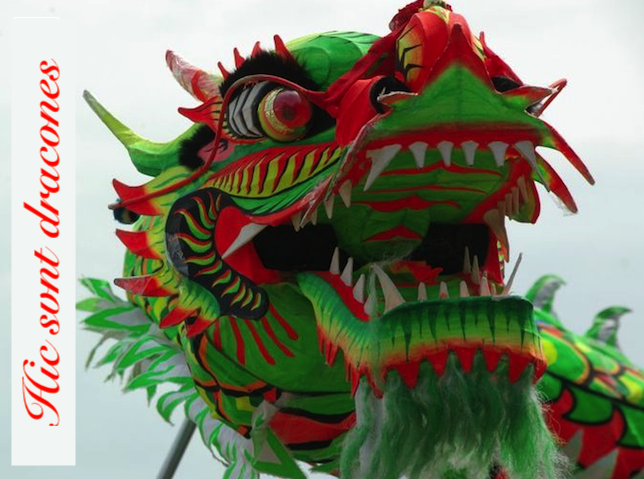
\includegraphics[width=0.75\textwidth]{imagenes/hic-svnt-dracones}
	\vspace{2cm}
	\begin{flushright}
		{\normalsize \textcolor{darkgray}{\textit{Ignacio Vallés Oriola}} \par}
	\end{flushright}
\end{titlepage}

\tableofcontents

\chapter*{}

%$ \ddot{x} \quad 	\displaystyle \dot{x} \quad  \va*{a} \quad \fdv{g} \quad \fdv{F}{g} \quad \fdv{V}(E-TS) \quad  \fdv*{F}{x}$

La \emph{mecánica clásica} es la rama de la física que estudia las leyes del comportamiento de cuerpos físicos macroscópicos (a diferencia de la mecánica cuántica) en reposo y a velocidades pequeñas comparadas con la velocidad de la luz (mecánica relativista).

En la mecánica clásica en general se tienen tres aspectos invariantes: el tiempo es absoluto, la naturaleza realiza de forma espontánea la mínima acción y la concepción de un universo determinado.


El primer desarrollo de la mecánica clásica suele denominarse \emph{mecánica newtoniana}. Consiste en los conceptos físicos basados en los trabajos fundacionales de Sir Isaac Newton, y en los métodos matemáticos inventados por Gottfried Wilhelm Leibniz, Joseph-Louis Lagrange, Leonhard Euler, y otros contemporáneos, en el siglo XVII para describir el movimiento de los cuerpos físicos bajo la influencia de un sistema de fuerzas. Posteriormente, se desarrollaron métodos más abstractos que dieron lugar a las reformulaciones de la mecánica clásica conocidas como \emph{mecánica lagrangiana} y \emph{mecánica hamiltoniana}. Estos avances, realizados predominantemente en los siglos XVIII y XIX, van sustancialmente más allá de los trabajos anteriores, sobre todo por su uso de la mecánica analítica. También se utilizan, con algunas modificaciones, en todas las áreas de la física moderna.

La mecánica clásica proporciona resultados extremadamente precisos cuando se estudian objetos grandes que no son extremadamente masivos y velocidades que no se acercan a la velocidad de la luz. Cuando los objetos que se examinan tienen el tamaño del diámetro de un átomo, se hace necesario introducir el otro gran subcampo de la mecánica: la mecánica cuántica. Para describir las velocidades que no son pequeñas en comparación con la velocidad de la luz, se necesita la relatividad especial. En los casos en los que los objetos se vuelven extremadamente masivos, se aplica la relatividad general. Sin embargo, algunas fuentes modernas incluyen la mecánica relativista en la física clásica, que en su opinión representa la mecánica clásica en su forma más desarrollada y precisa.

Existen varias formulaciones diferentes, en mecánica clásica, para describir un mismo fenómeno natural que, independientemente de los aspectos formales y metodológicos que utilizan, llegan a la misma conclusión.

La \emph{mecánica vectorial}, que deviene directamente de las leyes de Newton, por lo que también se le conoce como ``mecánica newtoniana'', llega, a partir de las tres ecuaciones formuladas por Newton y mediante el cálculo diferencial e integral, a una muy exacta aproximación de los fenómenos físicos. Es aplicable a cuerpos que se mueven en relación con un observador a velocidades pequeñas comparadas con la de la luz. Fue construida en un principio para una sola partícula moviéndose en un campo gravitatorio. Se basa en el tratamiento de dos magnitudes vectoriales bajo una relación causal: la fuerza y la acción de la fuerza, medida por la variación del momentum (cantidad de movimiento). El análisis y síntesis de fuerzas y momentos constituye el método básico de la mecánica vectorial. Requiere del uso privilegiado de sistemas de referencia inercial

La \emph{mecánica analítica} es una formulación matemática abstracta sobre la mecánica; permite desligarse de esos sistemas de referencia privilegiados y tener conceptos más generales al momento de describir un movimiento con el uso del cálculo de variaciones. Sus métodos son poderosos y trascienden de la mecánica a otros campos de la física. Se puede encontrar el germen de la mecánica analítica en la obra de Leibniz, quien propone que para solucionar problemas en mecánica, magnitudes escalares (menos oscuras según Leibniz que la fuerza y el momento de Newton), como energía cinética y el trabajo, son suficientes y menos oscuras que las cantidades vectoriales, como la fuerza y el momento, propuestos por Newton. Existen dos formulaciones equivalentes: la llamada \emph{mecánica lagrangiana} es una reformulación de la mecánica realizada por \emph{Joseph Louis Lagrange} que se basa en la ahora llamada ecuación de Euler-Lagrange (ecuaciones diferenciales de segundo orden) y el principio de mínima acción; la otra, llamada \emph{mecánica hamiltoniana}, es una reformulación más teórica basada en una funcional llamada hamiltoniano realizada por \emph{William Hamilton}. Las mecánicas hamiltoniana y lagrangiana son ejemplos de mecánicas analíticas, donde las magnitudes se relacionan entre sí por ecuaciones diferenciales parciales.\footnote{Fuente: wikipedia.}

\rule{250pt}{0.1pt}

Establecer las fuerzas reales que actúan en un problema puede llegar a ser bastante complicado, sobre todo si existen \emph{ligaduras} que limitan el rango de una o varias variables. Además, las \emph{ecuaciones de Newton} cambian de forma y no son invariables ante transformaciones de coordenadas (rotaciones, traslaciones, …).

Las formulaciones \emph{lagrangiana} y \emph{hamiltoniana} se crearon para resolver estas dificultades y proporcionar un aparato matemático más poderoso con el que enfrentarse a los problemas mecánicos.

\vspace{1cm}

\textbf{Estructura}

\begin{adjustwidth}{20pt}{20pt}
	\vspace{5mm} \begin{myblock}{Teoría destacada}
		
	\end{myblock}
	
	\vspace{5mm} \begin{myalertblock}{Resultados destacados}
		
	\end{myalertblock}
	
	\vspace{5mm} \begin{ejemplo} 
		\textbf{Aclaraciones de Javier García}, normalmente al final del capítulo.
		
		\textbf{Introducciones a cada tema}, al inicio de cada capítulo.
	\end{ejemplo}
	
	
	\vspace{5mm} \begin{myexampleblock}{Aclaraciones, curiosidades, ...}
		
	\end{myexampleblock}
	
		\vspace{5mm} \begin{ejercicio} \textbf{Ejercicios propuestos.} \end{ejercicio}

\end{adjustwidth}





\vspace{1cm}

\centering{
\fcolorbox{black}{fondoblau}{
\parbox{0.95\textwidth}{
	\textit{Este material es un conjunto de apuntes personales que comparto gratuitamente en la red. Se agradecería la comunicación de la detección de cualquier error.}
}}}
\justify


Basado en los vídeo cursos de física de Javier García Garrido, licenciado en Física y Máster en Gravitación y Partículas, en este caso en el de ``Mecánica Teórica'':

\begin{center} \textcolor{blue}{https://www.youtube.com/playlist?list=PLAnA8FVrBl8C-2TTrbArT1g04RJEckRMG} \end{center}




\emph{\normalsize{Este} documento se comparte bajo licencia `Attribution-NonCommercial 4.0 International (CC BY-NC 4.0)'}


\begin{multicols}{2}
\begin{figure}[H]
	\centering
	
\includegraphics[width=.4
	\textwidth]{imagenes/licencia.png}
	
\end{figure}
\begin{figure}[H]
	\centering
	
\includegraphics[width=.3
	\textwidth]{imagenes/firma.png}
\end{figure}
\end{multicols}

\newpage




\newpage

$\,$

\newpage

$\,$

\vspace{1cm} 

$\,$

\begin{figure}[H]
	\centering
	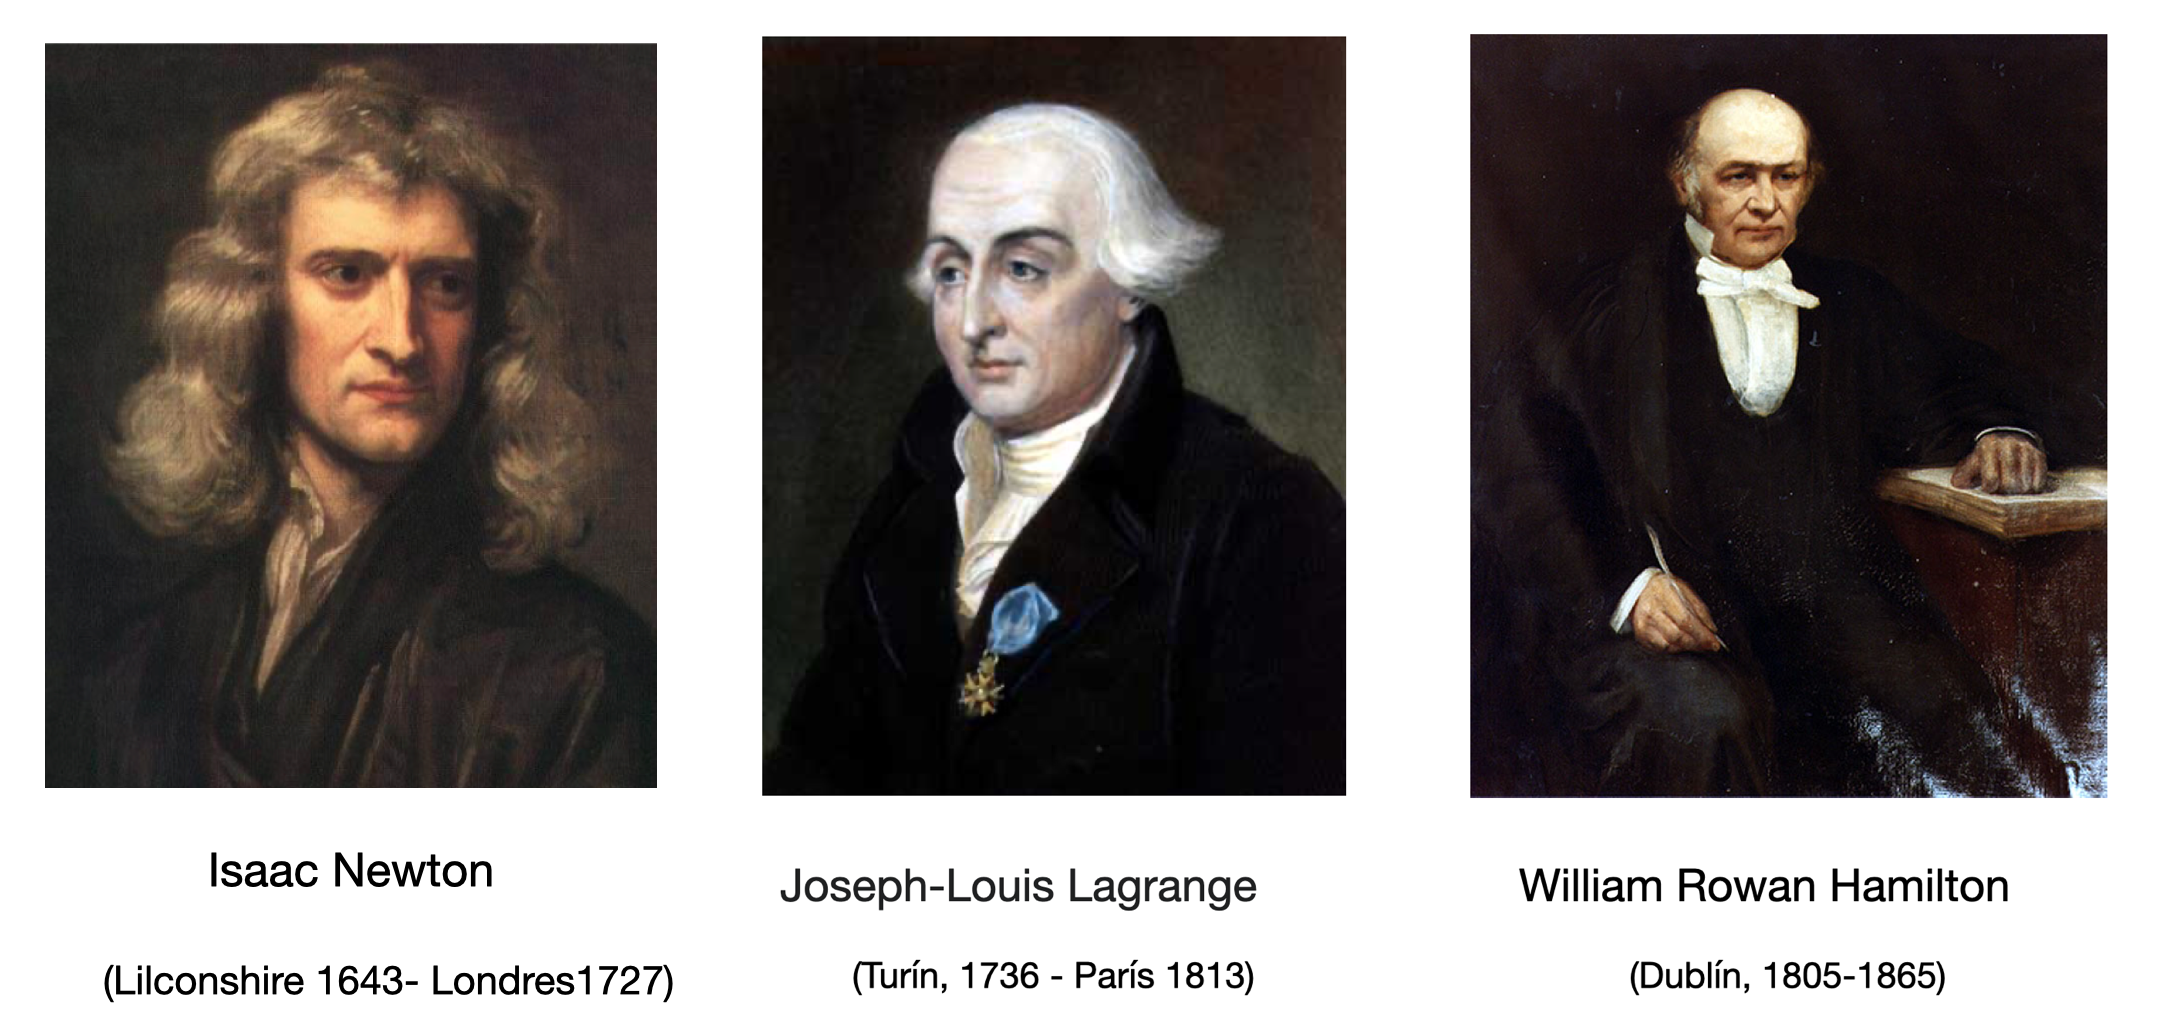
\includegraphics[width=.75\textwidth]{imagenes/portada.png}
\end{figure}


\begin{center}

\Huge{\textbf{Elementos clave de}}

\Huge{\textbf{Mecánica Teórica}} 


\large{\textbf{\textit{Video curso de Javier garcía}}}

\vspace{10mm}
\begin{figure}[H]
	\centering
	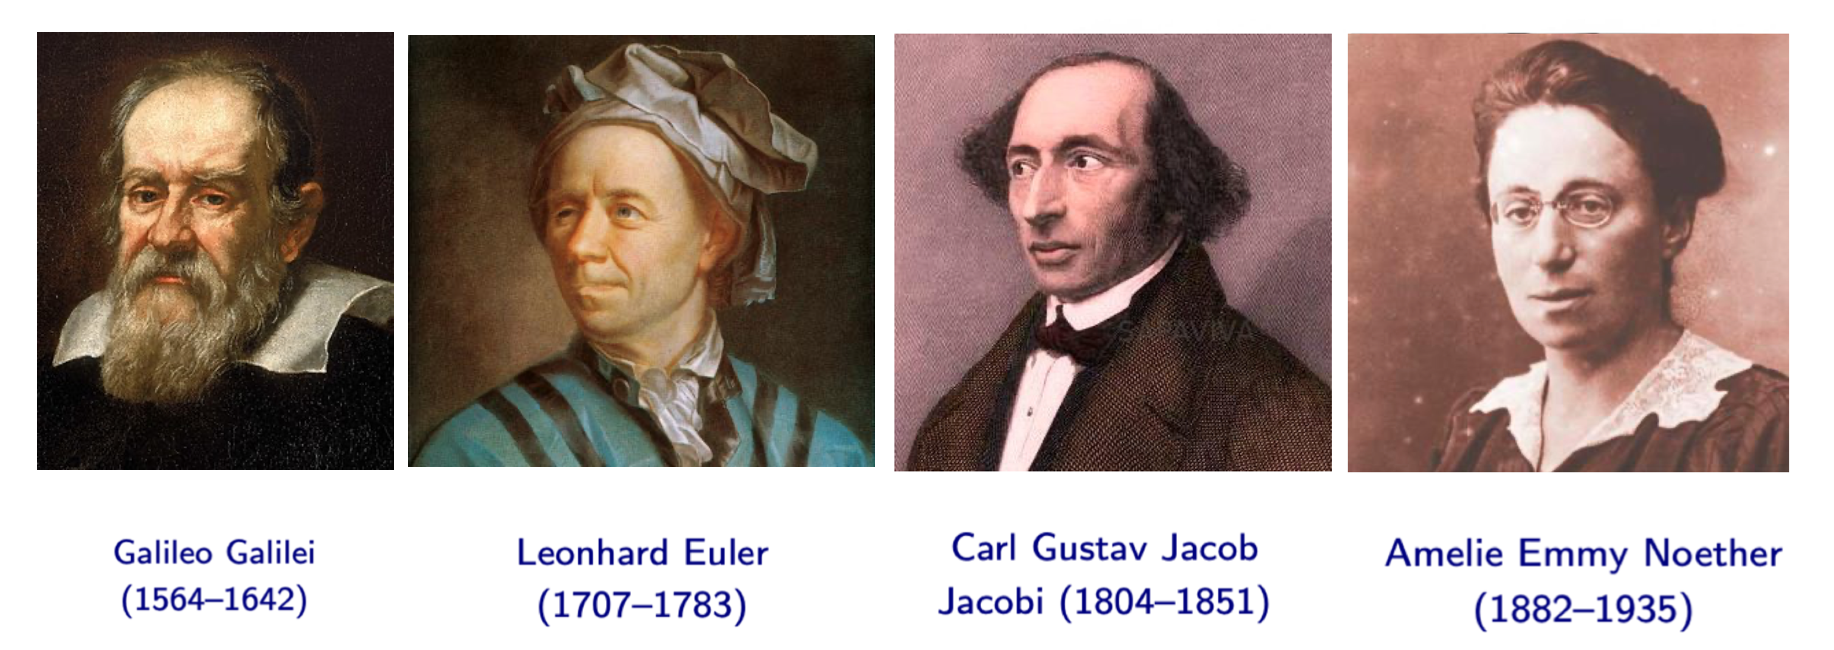
\includegraphics[width=.75\textwidth]{imagenes/portada2.png}
\end{figure}

\vspace{2cm}
\begin{flushright}
	\normalsize{\emph{Ignacio Vallés Oriola}}
\end{flushright}


\end{center}






\chapter{El principio de \emph{D'Alembert}}



	\begin{tikzpicture}
	\fill [left color=red!50, right color=teal!50] (0,0) rectangle (6.5,.1);
	\fill [left color=teal!50, right color=blue!50] (6.5,0) rectangle (11.5,.1);
	\end{tikzpicture}

\vspace{1cm}

\begin{adjustwidth}{50pt}{50pt}
\begin{ejemplo}
	En este tema veremos otro modo de resolver un sencillo problema de estática distinto a como se resuelve en mecánica newtoniana, usaremos el \emph{principio de D'Alembert}.	
\end{ejemplo}
\end{adjustwidth}
	
\vspace{1cm}
	
\section{Principio de \emph{D'Alembert} o de los Trabajos Virtuales}\label{T1PTV}

\vspace{0.5cm}

\begin{myblock}{Principio de D'Alembert para el caso estático}
$\,$

\begin{Large}
\begin{equation}
\label{DA}
 \displaystyle \sum_i \ \overrightarrow{F_i}^{(a)} \cdot \delta \overrightarrow{r_i}	 \ = \ 0
\end{equation}
\end{Large}
$\,$
\end{myblock}

\vspace{1cm}
\normalsize{Pronto} veremos el significado de esta ecuación. Empecemos analizando un sencillo ejemplo por dos métodos distintos: usando la conocida \emph{mecánica newtoniana} (ejemplo 1) y aplicando el \emph{Principio de D'Alembert o de los Trabajos Virtuales} (ejemplo 2).

\vspace{1cm}

\begin{example}
.	Determinar la \emph{fuerza de fricción} $F$ para que la barra rígida, uniforme y homogénea de masa $M$ y longitud $L$, apoyada en una esquina recta con ángulo $\theta$ se encuentre en equilibrio, \textbf{\emph{caso estático}}.

	\begin{figure}[H]
		\centering
		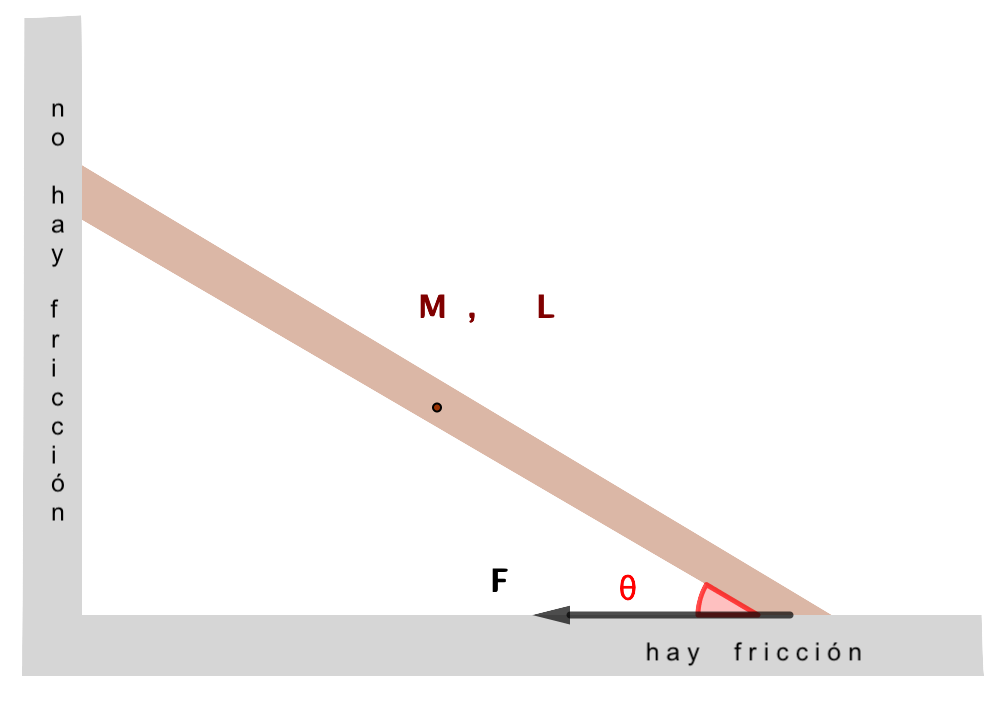
\includegraphics[width=.6\textwidth]{imagenes/img01-01.png}
	\end{figure}
	
	\begin{small}
	\textcolor{gris}{Hemos dibujado la fuerza de fricción, $F$, hacia la izquierda,  significando que se opone al movimiento.}	
	\end{small}

\end{example}

\vspace{1cm}
\subsection{Resolución por mecánica newtoniana}
\begin{tikzpicture}
	\fill [left color=red!50, right color=teal!50] (0,0) rectangle (3.5,.01);
	\fill [left color=teal!50, right color=blue!50] (3.5,0) rectangle (7.5,.01);
	\end{tikzpicture}
\vspace{0.5cm}

Las condiciones de equilibrio de la mecánica newtoniana son

\vspace{5mm}
\begin{myalertblock}{Mecánica newtoniana: equilibrio estático}

$\,$

\begin{Large}
\begin{equation}
\sum \ \overrightarrow F \ = \ \overrightarrow 0 
\quad ; \qquad \qquad 
\sum \ \overrightarrow M 	\ = \ \overrightarrow 0 
\end{equation}
\end{Large}
	
\end{myalertblock}


\vspace{5mm} La última de estas ecuaciones, para el caso bidimensional, podemos escribirla en módulos,  $\sum \ M = 0$, para lo cual tomaremos el siguiente convenio de signos: asignaremos el sentido \emph{positivo} si la barra tiende a moverse hacia la \emph{izquierda (sentido levógiro)} y \emph{negativo} si el movimiento es hacia la \emph{derecha (dextrógiro)}. Indicamos el sentido positivo con una flecha de giro azul en la figura siguiente.

Dibujamos las fuerzas que actúan:


\begin{adjustwidth}{10pt}{10pt}
--- Fuerza peso, $Mg$, situada en el centro de gravedad de la barra.

--- Fuerza de fricción, $F$, que se opone al movimiento.

--- Fuerzas de reacción (normales) de las paredes, $N_1 \ \text{ y } \ N_2$, que hacen que la barra no se hunda.
\end{adjustwidth}

\vspace{1cm}
	\begin{figure}[H]
		\centering
		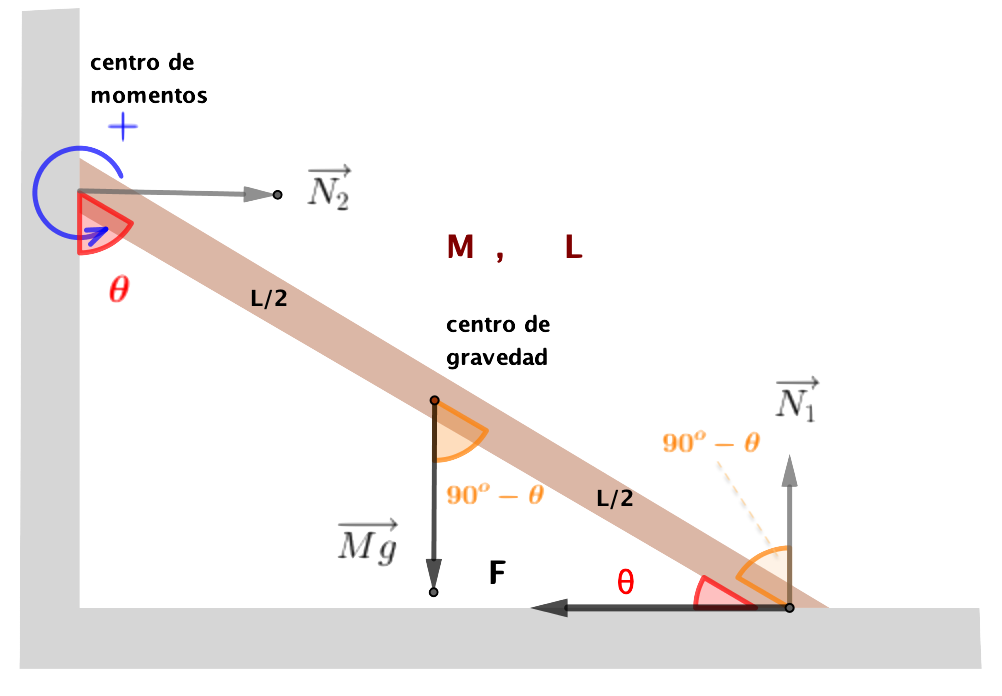
\includegraphics[width=.6\textwidth]{imagenes/img01-02.png}
	\end{figure}
	
\vspace{5mm}

$\boldsymbol{\displaystyle \sum \overrightarrow F = \overrightarrow 0} \ \ \to \ \ \overrightarrow N_2 + \overrightarrow {Mg} + \overrightarrow N_1 + \overrightarrow F = \overrightarrow 0$

Colocando en la esquina el sistema de referencia, 

$(N_2,0) + (0,-Mg)+(0,N_1)+(-F,0) \ \to \ \begin{cases}
\quad N_2-F=0 \\ \ -Mg+N_1=0 	
 \end{cases}
 \ \to \ $
 
 \begin{multicols}{2}
 \begin{equation}
\to \quad \boxed{ \  F = N_2 \ }
	\label{N1}
 \end{equation}
  \begin{equation}
; \qquad \qquad \boxed{ \  N_1 = Mg  \ } \qquad 
	\label{N2}
 \end{equation}
\end{multicols}

\textcolor{gris}{$\overrightarrow M = \overrightarrow F \times \overrightarrow F; \quad M=r\ F\ \sin \alpha$, siendo $\overrightarrow r$ el vector desde el eje (centro) de  momentos al punto de aplicación de cada fuerza $\overrightarrow F$ y  $\alpha$ el ángulo que forman $\overrightarrow r$ y $\overrightarrow F$}

Elegimos, arbitrariamente, el centro de momentos en el punto de aplicación de $\overrightarrow N_2$, punto de contacto de la barra con la pared vertical.

$\boldsymbol{\displaystyle \sum \overrightarrow M = \overrightarrow 0} \ \ \to \ $ 
$\cancelto{0}{N_2 \ 0 \ \sin (90^o-\theta)}-\dfrac L 2 \ Mg \sin (90^o-\theta)- L\ F\ \sin \theta + L \ N_1\ \sin (90^o -\theta)=0$

Despejando: $\ \sin (90^o-\theta)=\cos \theta \ \to \ N_1 \cos \theta = \dfrac 1 2 M g \cos \theta + F \sin \theta$, dividiendo por $\cos \theta$:

\begin{equation}
\boxed{ \ N_1 \ = \ \dfrac 1 2 M g \ + \ F \tan \theta \ }
\label{N3}	
\end{equation}

Nuestros datos eran $\ M, \ L \text{ y } \theta \ $ y nuestras incógnitas $\ N_1,\ N_2, \ \boldsymbol F.\ $ De las ecuaciones \ref{N1},  \ref{N2} y \ref{N3},  obtenemos:

\begin{large}
\begin{equation}
	\subrayado{ \ \boxed{\ \boldsymbol{ F \ = \ \dfrac{Mg}{2\tan \theta}} \ } \ }
\label{R1}	
\end{equation}
\end{large}


	

	

\vspace{0.5cm}
\subsection{Resolución por el principio de \emph{D'Alembert}}
\begin{tikzpicture}
	\fill [left color=red!50, right color=teal!50] (0,0) rectangle (3.5,.01);
	\fill [left color=teal!50, right color=blue!50] (3.5,0) rectangle (7.5,.01);
	\end{tikzpicture}
\vspace{0.5cm}

\begin{myexampleblock}{Desplazamientos virtuales. Principio de D'Alembert}

%\begin{ejemplo}
\begin{small}
Por \emph{desplazamiento virtual} infinitesimal de un sistema físico se entiende una variación de su configuración como resultado de cualquier cambio infinitesimal arbitrario $\ \boldsymbol{\var \vec r_i} \ $ de las coordenadas del sistema compatible con las fuerzas y ligaduras impuestas al mismo en un instante dado $ t $. Es un cambio infinitesimal del sistema de coordenadas que ocurre mientras el tiempo se mantiene fijo. Se le llama \emph{virtual} en vez de real dado que ningún desplazamiento real puede ocurrir sin que el tiempo avance (solo ocurren en nuestra imaginación). La condición de equilibrio es independiente del tiempo real, es como si congelásemos el tiempo.


\vspace{2mm}En la mecánica analítica el concepto de desplazamiento virtual solo es significativo cuando se analiza un sistema físico sujeto a ligaduras que restringen su movimiento. El desplazamiento virtual $\var r$  es un caso especial de desplazamiento infinitesimal (normalmente denotado por $\dd r$) que se refiere a un cambio infinitesimal en las coordenadas de posición de un sistema de manera que las ligaduras se satisfacen.



\begin{destacado}
\textbf{Principio de D'Alembert}. \footnote{Enunciado por Jean Le Rond D'Alembert en 1743, en su obra ``Tratado de la dinámica''.}

\emph{Para que un sistema de puntos materiales esté en equilibrio bajo la acción de un conjunto de fuerzas aplicadas es necesario y suficiente que sea nula la suma de los trabajos virtuales elementales efectuados por estas fuerzas para cualquier desplazamiento virtual de dicho sistema efectuado a partir de una posición de equilibrio.}
\end{destacado}

 
 \begin{equation*}
 \subrayado{\boxed{\ \boldsymbol{\sum_i \vec F_i\cdot \var \vec r_i}=0 \ }}	\qquad \qquad  \text{(ec. \ref{DA})}
 \end{equation*}


El trabajo total efectuado por las fuerzas aplicadas es nulo.

\end{small}
\begin{multicols}{2}
\begin{small}
La figura muestra una aplicación sencilla de este principio a un sistema de una sola partícula y una sola fuerza aplicada, el peso.

El punto $B$ no es un punto de equilibrio, pues en el desplazamiento virtual indicado en la figura el peso realiza trabajo. El punto $A$ si es de equilibrio, pues cualquier desplazamiento virtual es perpendicular al peso y, por tanto, el peso no realiza trabajo. 
\end{small}
\begin{figure}[H]
	\centering
	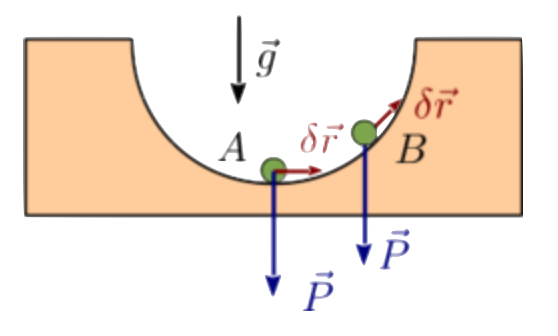
\includegraphics[width=.4\textwidth]{imagenes/img01-03.png}
\end{figure}
\end{multicols}

\begin{flushright}
\rule{200pt}{0.1pt}

\begin{scriptsize}
`Física General', Ignacio Vallés, \textcolor{blue}{http://igvaori.github.io}
\end{scriptsize}
\end{flushright}
%\end{ejemplo}
\end{myexampleblock}

\vspace{0.5cm}
Las condiciones de equilibrio el principio de D'Alembert (estático) es

\vspace{5mm}
\begin{myalertblock}{Principio de D'Alembert: equilibrio estático}

$\,$

\begin{Large}
\begin{equation*}
\sum_i \ \overrightarrow F_i^{(a)} \ \cdot \ \var \overrightarrow r_i \ = \ 0  \qquad \qquad  \text{(ec. \ref{DA})}
\end{equation*}
\end{Large}
	
\end{myalertblock}

\vspace{1cm}
$\overrightarrow N_1 \text{ y } \overrightarrow N_2$ son \emph{fuerzas restrictivas o de ligadura}, son las que no realizan trabajo ante un desplazamiento virtual de la barra, son perpendiculares a ellos. $\overrightarrow{Mg} \text{ y } \overrightarrow F$ son las \emph{fuerzas aplicados o externas}. Aplicando el principio de D'Alambert, tendremos:

\begin{multicols}{2}
$\,$

$\overrightarrow r_1=(L \cos \theta, 0);\quad \overrightarrow r_2= \left( \dfrac L 2 \cos \theta, \dfrac L 2 \sin \theta \right)$

$\displaystyle  \overrightarrow {\var r_1} = \pdv{\overrightarrow r_1}{L} \cancelto{0}{\var L}+ \pdv{\overrightarrow r_1}{\theta} \var \theta = \left( -\dfrac L 2 \sin \theta, \dfrac L 2 \cos \theta \right) \var \theta$

$\displaystyle  \overrightarrow {\var r_2} = \pdv{\overrightarrow r_2}{L} \cancelto{0}{\var L}+ \pdv{\overrightarrow r_2}{\theta} \var \theta = \left( - L  \sin \theta, 0 \right) \var \theta$
\begin{figure}[H]
	\centering
	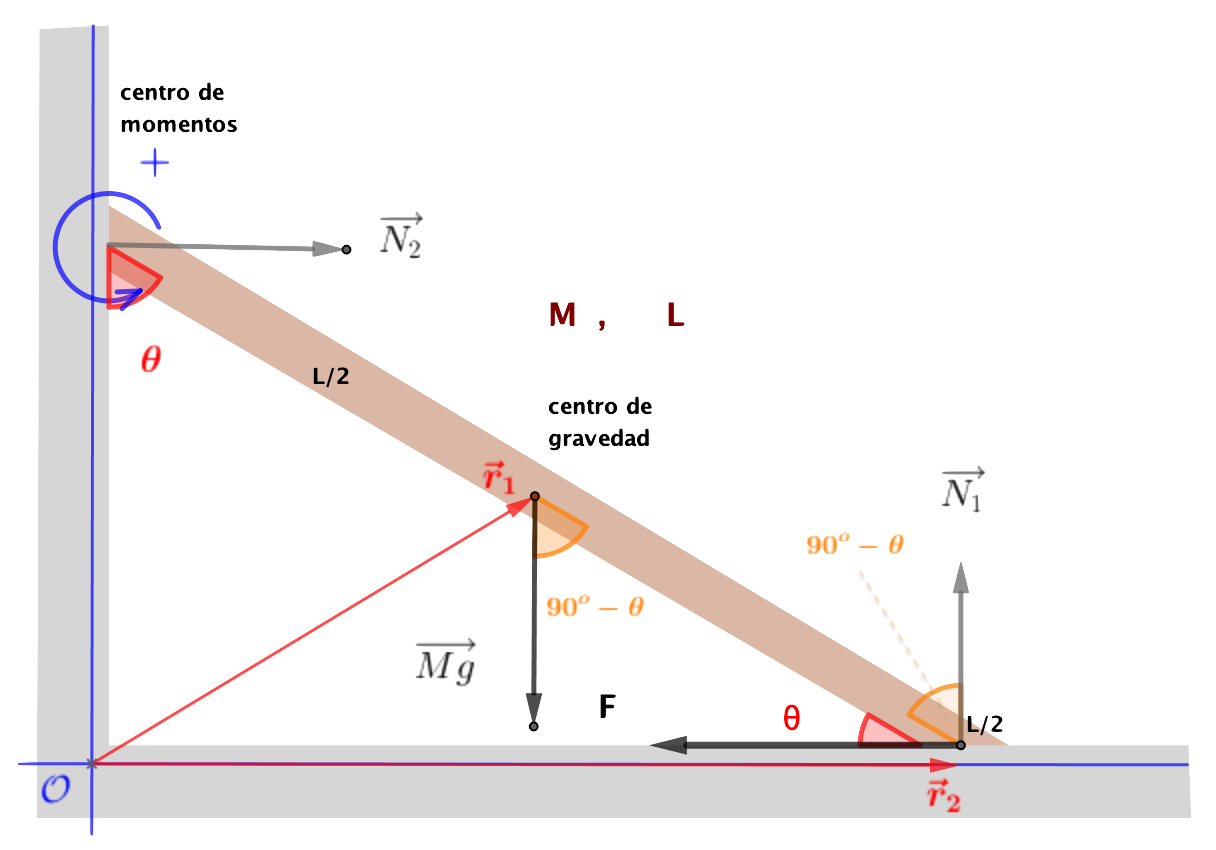
\includegraphics[width=.4\textwidth]{imagenes/img01-04.png}
\end{figure}
\end{multicols}

Ya que la longitud de la barra no varía en un desplazamiento virtual, $\ \var L = 0$, no sería compatible con las ligaduras.

Aplicando el principio de D'Alembert, tendremos:


$\overrightarrow{Mg} \cdot  \overrightarrow {\var r_1} + \overrightarrow F \cdot  \overrightarrow {\var r_2} =(0,-Mg)\cdot \left( -\dfrac L 2 \sin \theta, \dfrac L 2 \cos \theta \right) \var \theta +
(-F,0) \cdot  \left( - L  \sin \theta, 0 \right) \var \theta =0$

$-\dfrac{MgL}2 \cos \theta \ \var \theta + FL\sin \theta \ \var \theta =0$
$\ \to \ $
$\cancelto{\neq 0}{L} \ \left[ -\dfrac{Mg}{2} \cos \theta+ F \sin \theta \right] \ \cancelto{\neq 0}{\var \theta }= 0$

La barra tiene una determinada longitud no nula ($\cancelto{\neq 0}{L}$) y, por hipótesis, estamos considerando un desplazamiento virtual no nulo ($\cancelto{\neq 0}{\var \theta}$). Despejando, obtenemos el mismo resultado que aplicando la mecánica newtoniana:

\begin{large}
\begin{equation}
	\subrayado{ \ \boxed{\ \boldsymbol{ F \ = \ \dfrac{Mg}{2\tan \theta}} \ } \ }
\label{R1}	
\end{equation}
\end{large}







\chapter{Ecuaciones de \emph{Euler-Lagrange}}
\label{CapEEL}

	\begin{tikzpicture}
	\fill [left color=red!50, right color=teal!50] (0,0) rectangle (6.5,.1);
	\fill [left color=teal!50, right color=blue!50] (6.5,0) rectangle (11.5,.1);
	\end{tikzpicture}

\vspace{1cm}


\begin{adjustwidth}{50pt}{50pt}
\begin{ejemplo}
	Estudiaremos ahora el \emph{Principio de D'Alembert \textbf{dinámico}} y  deduciremos las ecuaciones \emph{Euler-Lagrange} como se hizo históricamente (no usando cálculo variacional).	
\end{ejemplo}
\end{adjustwidth}
	
\vspace{0.5cm}

\section{Principio de \emph{D'Alembert} dinámico}

\vspace{0.5cm}

\begin{myblock}{Principio de D'Alembert para el caso dinámico}
$\,$

\begin{Large}
\begin{equation}
\label{DAD}
 \displaystyle \sum_i \ \left( \dot{ \ \overrightarrow p_i}\ - \ \overrightarrow{F_i}^{(a)} \right ) \cdot \delta \overrightarrow{r_i}	 \ = \ 0
\end{equation}
\end{Large}
$\,$
\end{myblock}

Recuérdese que $\ \displaystyle \overrightarrow p =m\overrightarrow v\ $ es la cantidad de movimiento y  

$\displaystyle  \dot{\overrightarrow p}=\dv{t} (m\overrightarrow v) = \textcolor{gris}{(m=cte)} = m\dv{\overrightarrow v}{t}=m \overrightarrow a$ es la 2a ley de Newton.

Otra forma de escribir la ecuación \ref{DAD}, considerando la cantidad de movimiento es:

\begin{myalertblock}{Principio de D'Alembert para el caso dinámico}	
\begin{large}
\begin{equation}
\label{DAD2}
\boldsymbol{ \displaystyle \sum_i \ \left( m \overrightarrow a_i \ - \ \overrightarrow{F_i}^{(a)} \right ) \cdot \delta \overrightarrow{r_i}	 \ = \ 0 }
\end{equation}
\end{large}
\end{myalertblock}

En un sistema de partículas, el subíndice $\boldsymbol i$ hace referencia a cada una de las partículas que componen el sistema, en el caso de un sólido rígido, $\boldsymbol i$ hace referencia a ls puntos donde se aplican las fuerzas.

Resolveremos un mismo ejemplo-problema de tres formas distintas: 1 - por Newton, 2 - por D'Alembert y 3 - con las ecuaciones de Euler-Lagrange.

\vspace{1cm}
\begin{example}
.	Partícula que se mueve libremente a lo largo de una barra.

\begin{figure}[H]
	\centering
	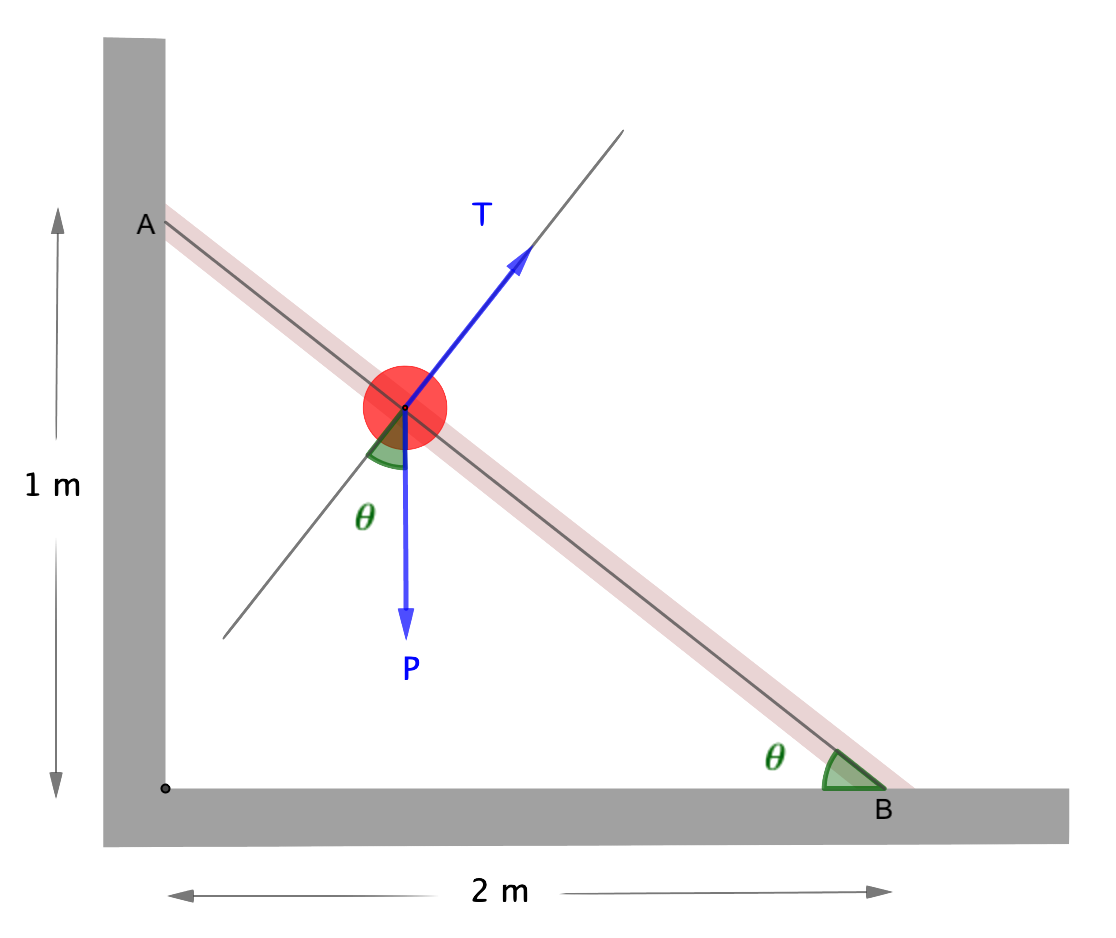
\includegraphics[width=.6\textwidth]{imagenes/img02-01.png}
\end{figure}
\end{example}

\vspace{1cm}
\subsection{Resolución por \emph{Newton}}
\begin{tikzpicture}
	\fill [left color=red!50, right color=teal!50] (0,0) rectangle (3.5,.01);
	\fill [left color=teal!50, right color=blue!50] (3.5,0) rectangle (7.5,.01);
	\end{tikzpicture}
	
\vspace{0.5cm}
Suponemos que no hay fricción. Las únicas fuerzas que actúan son el peso, $\overrightarrow P$, y una fuerza de reacción de la barra, que se opone al movimiento y es perpendicular a la superficie de contacto, $\overrightarrow T$. Usamos como sistema de referencia el centrado en la partícula que se mueve y cuyo eje x es solidario con la barra sobre la que se desplaza la partícula:

$\overrightarrow T=(0,T);\quad \overrightarrow P=(mg\sin \theta, -mg \cos \theta)$

Aplicando la 2a de Newton:

$\displaystyle \boldsymbol{ \sum_i  \overrightarrow F_i =m\overrightarrow a } \ \to \ (0,T)+(mg\sin \theta, -mg \cos \theta)=m\overrightarrow a$

$(mg\sin \theta, T-mg \cos \theta)=m(a_x,a_y) \ \to \ \begin{cases}
 \ a_x=g\sin \theta	 \\ \ a_y=(T-mg \cos \theta) / m
 \end{cases}$

Como a partícula está obligada a moverse a lo largo del eje x, no hay movimiento en el eje y: $\ a_y = 0 \ \to \ $

\begin{multicols}{2}
\begin{equation}
T \ = \ mg\cos \theta	
\end{equation}

\begin{equation}
a_x \ = \ g \sin \theta	
\end{equation}
\end{multicols}

Calculemos, ahora, el tiempo que tarda nuestra partícula en recorrer toda la barra, desde el punto A hasta el B.

$a_x=g\sin \theta = cte \ \to \ MRUA \ \to \ x=\cancelto{0}{x_0}+ \cancelto{0}{v_0}t+\dfrac 1 2 a_x t^2=\dfrac 1 2 g \sin \theta t^2$

De la figura, puesto que $\theta$ es el ángulo de un triángulo rectángulo de cateto opuesto $2$ y cateto contiguo $1$ (hipotenusa $\sqrt{5}$), se tiene que $\sin \theta = 2/\sqrt{5}$, tomando $g\approx 10$ ms$^{-2}$, obtenemos:

$x=\dfrac 1 2 \ 10 \ \dfrac 2 {\sqrt{5}} t^2 = \dfrac {12}{\sqrt
5} t^2$

Al recorrer la partícula toda la longitud de la barra, $\sqrt
5$, obtendremos finalmente que el tiempo empleado es: \textcolor{gris}{$\left( \sqrt{5}=\dfrac {12}{\sqrt
5} t^2 \ \to \ 5=10 t^2 \right)$}

\begin{equation}
\label{R2MN}
\subrayado{ \ \boxed{ \ 
	t \ = \ \dfrac 1 {\sqrt{2}} \ \mathrm{s}
\ } \ }
\end{equation}

\vspace{1cm}
\subsection{Resolución por \emph{D'Alembert}}
\begin{tikzpicture}
	\fill [left color=red!50, right color=teal!50] (0,0) rectangle (3.5,.01);
	\fill [left color=teal!50, right color=blue!50] (3.5,0) rectangle (7.5,.01);
	\end{tikzpicture}
%\vspace{0.5cm}

La única fuerza aplicada es el $\overrightarrow P$, la $	\overrightarrow T$ es una fuerza de ligadura (restrictiva), por lo que el principio de D'Alembert \emph{dinámico} dice que:

\begin{equation}
\label{PDDT2E}
\boldsymbol{
	( \ m\overrightarrow a \ - \ \overrightarrow P \ ) \ \cdot \ \overrightarrow {\var r	} \ =  \ 0
}
\end{equation}

%\vspace{5mm}
\begin{multicols}{2}
\begin{figure}[H]
	\centering
	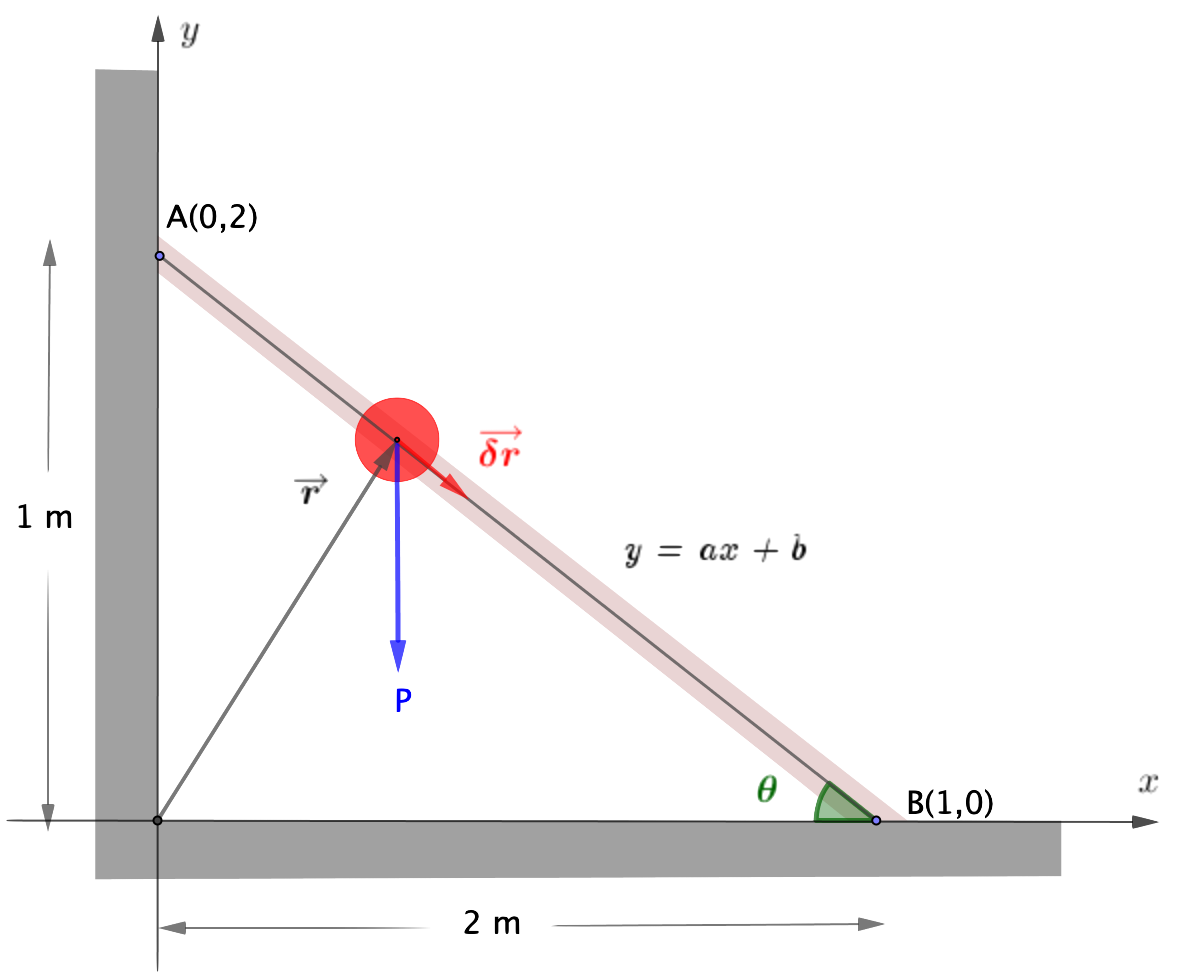
\includegraphics[width=.4\textwidth]{imagenes/img02-02.png}
\end{figure}


Para calcular el desplazamiento virtual $\overrightarrow{\var r}$, vamos a \emph{parametrizar} la recta por la que está obligada a moverse la partícula: $\ y=ab+b$, que pasa por los puntos $A(0,2)$ y $B(1,0)$.

$A(0,2):\ \  2=a\cdot 0 + b \to b=2$

$B(1,0):\ \ 0=a\cdot 1 + 2 \to a=-2$

La recta buscada es: $\ y=-2x+2$ 
\end{multicols}



\begin{equation}
\label{paramT2}
\text{\emph{Parametrización:}}\quad 
\begin{cases}
\ x\ = \ q \\ \ y \ = \ -2q+2
\end{cases} ; \qquad q \in [0,1] \subset \mathbb R
\end{equation}

A medida que varía $q \in [0,1]$ variará la $\overrightarrow r$ y la partícula se moverá siempre por la barra.

$\begin{cases} 
	 \displaystyle \ \var x = \pdv{x}{q} \var q = 1\cdot \var q \\ \displaystyle \ \var y = \pdv{y}{q} \var q = -2  \cdot \var q
\end{cases} \to \quad \overrightarrow{\var r} = (1,-2) \ \var q $

Llevando este resultado y sabiendo que $\ \overrightarrow P=(0,-P)\ $ a la ecuación del principio de D'Alembert dinámico\ref{PDDT2E}, tenemos:

$(ma_x,ma_y-(-mg)) \cdot (1,-2) \ \var q =0 \to \cancelto{\neq 0}{m} \ (a_x-2(a_y+g)) \ \cancelto{\neq 0} {\var q} = 0$, por lo que

\begin{equation}
\label{R2PDD}
\boxed{ \ a_x \ = \ 2 (a_y+g) \ }	
\end{equation}

Relación que, de momento, no se asemeja demasiado al resultado obtenido aplicando la mecánica newtoniana, ec. \ref{R2MN}.

Vamos a derivar (dos veces) las ecuaciones de la parametrización, ec \ref{paramT2}:

$\begin{cases}
\ x =  q \\ \ y  = -2q+2
\end{cases} \to \qquad \begin{cases}
 \  \dot x = \dot q \\ \ \dot y = -2 \dot q
 \end{cases} \to \qquad \begin{cases}
 \ \ddot x= \ddot q =a_x	 \\ \ \ddot y=-2\ddot q = a_y
 \end{cases}$

Sustituyendo en ec. \ref{R2PDD}, tenemos: $\ \ddot q=2(-2\ddot q +g) \ \to \ 5\ddot q= 2g$, por lo que, con $g\approx 10 \ \mathrm{ms}^{-2}$,

\begin{equation}
\ddot q = 4	
\end{equation}

Integramos, ahora (dos veces) para encontrar $q(t)$

$\ddot q(t) = \displaystyle \int \ddot q \ \dd t = \int 4 \ \dd t = 4t +K$

$q(t)= \displaystyle \int \dot q \ \dd t = \int (4t+K) \ \dd t = 2t^2 +Kt+C$

Impongamos las condiciones iniciales:

$t=0: \ A(x=0,y=2)  \ \to \ q(0)=x(0)=0=2\cdot 0^2 + K\cdot o + C \to C=0$

$t=0: \ $ \begin{tiny} {(partícula se mueve libremente)} \end{tiny} $ \ \dot q(0)=v_x(0)=0 \ \to \ 0=4\cdot 0 + K \to K=0$

Luego, $\ q(t)=2t^2$ y, con ello,

\begin{equation}
\label{R3PDD}	
\begin{cases}
	\ x \ = \ \textcolor{gris}{q} \ = \ 2t^2 \\
	\ y \ = \ \textcolor{gris}{-2q+2} \ = \  -4t^2+2
\end{cases}
\end{equation}

Ecuaciones cuya solución es equivalente a la que hemos obtenido al aplicar la mecánica newtoniana.

Como comprobación, calcularemos el tiempo que tarda la partícula en recorrer toda la barra.

Al llegar al suelo, $\ y=0=-4t^2+2$, despejando:

\begin{equation}
\label{RFPDD}
\subrayado {\ \boxed{ \ \ t \ = \ \dfrac{1}{\sqrt{2}}	\ \mathrm{s} \ } \ }
\end{equation}

Resultado que, evidentemente, coincide con el obtenido con Newton, ec. \ref{R2MN}.

Parece que esto no sea más que complicarse absurdamente la existencia, pero en el caso de que hayan \emph{ligaduras}, el método de Newton es ardua, en cambio, \emph{parametrizando} el vector de posición respecto de unas variables que llamaremos \emph{``variables generalizadas''} hará que todo sea mucho más sencillo.

Vamos ahora a introducir las \emph{ecuaciones de Euler-Lagrange} que nos facilitarán aún más el cálculo y volveremos a resolver por tercera vez el problema-ejemplo de la partícula en la barra.


\vspace{1cm}
\section{Ecuaciones de \emph{Euler-Lagrange}}
\begin{tikzpicture}
	\fill [left color=red!50, right color=teal!50] (0,0) rectangle (3.5,.01);
	\fill [left color=teal!50, right color=blue!50] (3.5,0) rectangle (7.5,.01);
	\end{tikzpicture}
\vspace{0.5cm}

Por sencillez, consideraremos el caso de solo una partícula cuya trayectoria se puede parametrizar con un solo parámetro (grado de libertad), q, que recibe n el nombre de \textbf{\emph{coordenadas generalizadas}}.

Vamos a pasar del principio de D'Alembert dinámico a las ecuaciones de Euler-Lagrange, partimos de:

$$\displaystyle \sum_i \left ( \ \dot{\ \overrightarrow p_i} - \overrightarrow F^{(a)}_i \ \right) \ \cdot \ \overrightarrow{\var r_i} \ = \ 0$$

De otro modo: $\qquad   (\dot{\ \overrightarrow p} - \overrightarrow F)\cdot \overrightarrow {\var r} = 0 \ \to \dot{\ \overrightarrow p}\cdot \overrightarrow{\var r} = \overrightarrow F \cdot \overrightarrow{\var r}$

El vector de posición dependerá del parámetro $q$ y, tal vez, del tiempo $t$: $\quad \overrightarrow r= \overrightarrow r (q,t)$.

\begin{small}
\textcolor{gris}{Obviamente, la parametrización ha de satisfacer las condiciones de ligadura:}

\textcolor{gris}{Circunferencia radio $R$: $\ \begin{cases} \ x=R \cos q \\ \ y=R \sin q \end{cases}$; $\quad$ Nuestra barra: $\ \ \begin{cases} \ x=q \\ \ y=-2q+2 \end{cases}$; $\quad$ etc.}
\end{small}


Como $\ \dot{\ \overrightarrow p}=m\dot{\ \overrightarrow v} \ \text{ y }  \ \displaystyle \overrightarrow{ \var r} = \pdv{\overrightarrow r}{q} \var q \ , \ \  \qquad m \dot{\ \overrightarrow v} \cdot \pdv{\overrightarrow r}{q} \var q = \overrightarrow F \cdot \pdv{\overrightarrow r}{q} \var q $

Por \textbf{definición}, llamamos \textbf{\emph{fuerza generalizada}}, $\boldsymbol {Q}$, a la expresión siguiente cuyo sentido encontraremos más adelante:

\begin{equation}
\label{T2FG}	
\boxed{ \ \overrightarrow F \ \cdot \ \pdv{\overrightarrow r}{q}\ =  \ Q \ }
\end{equation}

Con lo que, de momento, el principio de D'Alembert dinámico nos queda como:

\begin{equation}
\label{T2PDD2}
m \dot{ \ \overrightarrow v} \ \cdot \ 	\pdv{\overrightarrow r}{q} \ \ \overrightarrow{\var q} \ = \ Q\ \var q
\end{equation}

Analicemos la primera parte de esta ecuación, $\displaystyle \ m \dot{ \ \overrightarrow v}  \cdot 	\pdv{\overrightarrow r}{q}$, para $m=cte$,

$$\displaystyle m \dot{ \ \overrightarrow v} \cdot \pdv{\overrightarrow r}{q} = \dv{t} \, (m\overrightarrow v)\cdot \pdv{\overrightarrow r}{q}$$

Desarrollemos la expresión: $\displaystyle \ \ \dv{t} \left[ m \overrightarrow v \cdot \pdv{\overrightarrow r}{q} \right] = 
 \dv{t} \, (m\overrightarrow v)\cdot \pdv{\overrightarrow r}{q} +
 m \overrightarrow v \cdot \dv{t} \left( \pdv{\overrightarrow r}{q} \right)   $
 
 
 \begin{equation}
 \label{T2PDD3}
 \text{Despejando: } \qquad \qquad 
 \dv{t} (m\overrightarrow v) \cdot \pdv{\overrightarrow r}{q} \ = \ 	
 \dv{t} \left[ m \overrightarrow v \cdot \pdv{\overrightarrow r}{q} \right] -
 m \overrightarrow v \cdot \dv{t} \left( \pdv{\overrightarrow r}{q} \right)
 \end{equation}

 
\rule{150pt}{0.1pt}

\underline{Inciso 1}:  $\quad$ como $\displaystyle \ \ \overrightarrow v= \dv{t} \overrightarrow r(q,t)= \pdv{\overrightarrow r}{q} \ \dv{q}{t} + \pdv{\overrightarrow r}{t}$

\textcolor{gris}{Ejemplo: $\ x=q^2+\sin t \to v=2q\dv{q}{t}+\cos t=2q\dot q+\cos t$}

\textcolor{gris}{Es como la regla de la cadena: $\ \dv{x}{t} = \dv{t} (q^2) + \dv{t} (\sin t) = 2q\dot q + \cos t$}

\begin{flushright}
\rule{200pt}{0.1pt}	
\end{flushright}

Teniendo en cuenta lo visto en el inciso 1,

\begin{equation}
\label{T2PDD4}
\boldsymbol{ \overrightarrow v \ = } \ \textcolor{gris}{ \dv{\overrightarrow r}{t} } \ \boldsymbol{ = \ \pdv{\overrightarrow r}{q}\ \dot q \  + \   \pdv{\overrightarrow r}{t} }
\end{equation}

Derivando respecto de $\dot q$: $\quad \displaystyle \pdv{\overrightarrow v}{\dot q} \ = \ \pdv{\dot q} \left( \pdv{\overrightarrow r}{q} \ \dot q \right) + \pdv{\dot q} \left(\pdv{\overrightarrow r}{t} \right) $

Aplicamos el \emph{teorema de Schwarz} para funciones continuas con derivadas continuas: `se puede cambiar el orden de derivación':

$\displaystyle \pdv{\overrightarrow v}{\dot q} \ = \ \pdv{\dot q} \left( \pdv{\overrightarrow r}{q} \ \dot q \right) + \pdv{ t} \cancelto{0}{\left(\pdv{\overrightarrow r}{\dot q} \right)} \, , \ \ $ ya que $\overrightarrow r=\overrightarrow r(q,t) \to  \neq \overrightarrow r(\dot q)$

Así pues, $\quad \displaystyle \boldsymbol{ \pdv{\overrightarrow v}{\dot q} } \ = \ \pdv{\dot q} \left( \pdv{\overrightarrow r}{q} \ \dot q \right) =
\cancelto{0}{\pdv{\dot q} \left( \pdv{\overrightarrow r}{q} \right)} \dot q + \pdv{\overrightarrow r}{q} \ \cancelto{1}{\pdv{\dot q}{\dot q} } = \boldsymbol{ \pdv{\overrightarrow r}{q} }$

Donde hemos tenido en cuenta la derivada del producto y que como

$\displaystyle \overrightarrow r = \overrightarrow r(q,t) \to \pdv{\overrightarrow r}{t}=\pdv{\overrightarrow r}{t} \ (q,t) \neq  \pdv{\overrightarrow r}{t} \ (\dot q)$%\ (q,t) \neq \pdv{\overrightarrow r}{t}  \ (\dot q)$

\begin{multicols}{2}
Destacamos este último resultado:	

\begin{equation}
\label{T2UR1}
\pdv{\overrightarrow v}{\dot q} \ = \ \pdv{\overrightarrow r}{q} 
\end{equation}
\end{multicols}

\rule{150pt}{0.1pt}

\underline{Inciso 2}:  $\quad \text{como: } \ \ \displaystyle \dv{t} \ A \ = \ \pdv{A}{B} \cdot \dv{B}{t} \ + \ \pdv{A}{t} $ , 

invirtiendo el orden $\displaystyle \dv{t} \ A \ = \ \dv{B}{t} \cdot  \pdv{A}{B} \ + \ \pdv{A}{t} \ $ y tomando $\ A=\displaystyle \pdv{\overrightarrow r}{q};\ \ B=q$,
$\displaystyle 	\dv{t} \ \left( \pdv{\overrightarrow r}{q}\right) 
= \dv{q}{t} \cdot \pdv{q} \left( \pdv{\overrightarrow r}{q} \right)  +
\pdv{t} \left( \pdv{\overrightarrow r}{q}  \right)=
\dot q \cdot \pdv{q} \left( \pdv{\overrightarrow r}{q} \right)  +
\pdv{q} \left( \pdv{\overrightarrow r}{t}  \right)$

donde hemos aplicado al último término el teorema de Schwarz.

Teniendo en cuenta la derivada de la suma y que $\ \dot q \neq \dot q(q)$,

$\displaystyle 	\dv{t} \ \left( \pdv{\overrightarrow r}{q}\right) 
= \pdv{q} \left( \dot q \ \pdv{\overrightarrow r}{q} \right) + \pdv{q} \left( \pdv{\overrightarrow r}{t} \right) =
\pdv{q} \left[ 
\dot q \ \pdv{\overrightarrow r}{q} + \pdv{\overrightarrow r}{t} \right]= \pdv{\overrightarrow v}{q} $

En la última igualdad hemos tenido en cuenta la ecuación \ref{T2PDD4}

\begin{flushright}
\rule{200pt}{0.1pt}	
\end{flushright}

\begin{multicols}{2}
Destacamos, también, este último resultado:	

\begin{equation}
\label{T2UR2}
\dv{t} \ \left( \pdv{\overrightarrow r}{q}\right) \ = \ \pdv{\overrightarrow v}{q}
\end{equation}
\end{multicols}

Volviendo, con estos resultados ( ec. \ref{T2UR1} y ec. \ref{T2UR2} ), a la ecuación \ref{T2PDD3}, en que analizábamos un trozo del primer miembro de la aplicación del principio de D'Alembert dinámico para una coordenada generalizada y una fuerza generalizada, tenemos:

\begin{equation}
\label{T2PDD6}
\displaystyle \dv{t} \ (m\overrightarrow v) \cdot \pdv{\overrightarrow r}{q}=
\dv{t} \left[ m\overrightarrow v \cdot \pdv{\overrightarrow v}{\dot q} \right]-
m\overrightarrow v \cdot \pdv{\overrightarrow v}{q}\ \ \ 
\quad \text{ Ya lo tenemos casi.}
\end{equation}

\rule{150pt}{0.1pt}

\underline{Inciso 3}.  Truco: derivada del producto.

$\displaystyle \pdv{a} \ (\vec v \cdot \vec v) = \pdv{\vec v}{a} \cdot \vec v + \vec v \cdot \pdv{\vec v}{a} = 2 \vec v \cdot \pdv{\vec v}{a}$

es decir, $\displaystyle \ \vec v \cdot \pdv{\vec v}{a} = \dfrac 1 2 \pdv{a} \ ( \vec v \cdot \vec v )= \dfrac 1 2 \pdv{a} ( |\vec v|\ |\vec v|\cos 0^o )  = \dfrac 1 2 \pdv{a} \ v^2$


multiplicando por $\displaystyle m\ \ \ m \vec v \cdot \pdv{\vec v}{a} = m \dfrac 1 2 \pdv{a} v^2 = \ \textcolor{gris}{(m=cte)} \ = \dfrac 1 2 \pdv{a} (\dfrac m 2 v^2)$

\begin{flushright}
\rule{200pt}{0.1pt}	
\end{flushright}

Aplicando el resultado del inciso 3 al caso $ \ \displaystyle a=\dot q \  \to \  m\vec v \cdot \pdv{\vec v}{\dot q}= \pdv{\dot q} \left( \dfrac 1 2 m v^2 \right) $

Aplicando el resultado del inciso 3 al caso $ \ \displaystyle a= q \  \to \  m\vec v \cdot \pdv{\vec v}{ q}= \pdv{ q} \left( \dfrac 1 2 m v^2 \right) $

Incorporando estos resultados a la ec. \ref{T2PDD6}, tenemos:

$\displaystyle \dv{t} (m\vec v) \cdot \pdv{\vec r}{q} = \dv{t}
\left( \pdv{\dot q} \left( \dfrac 1 2 m v^2 \right) \right)-
\pdv{q} \left( \dfrac 1 2 m v^2 \right)$

Llamando $T$, \textbf{\emph{energía cinética}} a $\quad \boldsymbol{T \ = \ \dfrac 1 2 \ m v^2}\ ,$

$\displaystyle \dv{t} (m\vec v) \cdot \pdv{\vec r}{q} \ = \ \dv{t} \left[ \pdv{T}{\dot q} \right] - \pdv{T}{q}$

Volviendo al principio, ec \ref{T2PDD2}, principio de D'Alembert dinámico con una coordenada generalizada y una fuerza generalizada,

$\displaystyle \left[
\dv{t} \left( \pdv{T}{\dot q} \right) - \pdv{T}{q}
\right] \ \var q \ = \ Q \ \var q\ .\quad$ Como $\ \var q \neq 0\ ,$

\begin{equation}
\label{T2PDD7}
\boxed{ \ 
\dv{t} \left( \pdv{T}{\dot q} \right) \ - \ \pdv{T}{q} \ = \ Q \ = \ \overrightarrow F \cdot \pdv{\vec r}{q}	
\ }
\end{equation}

Ecuación válida para una partícula con un sólo grado de libertad, q (una sóla coordenada generalizada). Es válida para cualquier fuerza aplicada (aún de fricción), no solo para fuerzas conservativas aunque sean estas las más interesantes desde el punto de vista de la física teórica, por ello, veamos el caso de que la fuerza aplicada sea conservativa.

\vspace{1cm}
\subsection{Ecuaciones de \emph{Euler-Lagrange} para el caso conservativo}
\begin{tikzpicture}
	\fill [left color=red!50, right color=teal!50] (0,0) rectangle (3.5,.01);
	\fill [left color=teal!50, right color=blue!50] (3.5,0) rectangle (7.5,.01);
	\end{tikzpicture}
\vspace{0.5cm}


Es sabido que en un caso conservativo\footnote{Aclaración al final del capítulo.}, $\overrightarrow \nabla \times \overrightarrow F = \overrightarrow 0 \ \to \ \overrightarrow F = - \overrightarrow \nabla V$, la fuerza proviene de un potencial escalar $V(\overrightarrow r, t)$, $\displaystyle \ \overrightarrow F = -\left( \pdv{V}{x},\pdv{V}{y},\pdv{V}{z} \right)$

$\displaystyle \overrightarrow F \cdot \pdv{\overrightarrow r}{q} = - 
\left( \pdv{V}{x} \pdv{x}{q},\pdv{V}{y} \pdv{y}{q},\pdv{V}{z} \pdv{z}{q} \right) = - \pdv{V}{q}\ , \ \ $ por la regla de la cadena. 

Por ello, $\ \displaystyle \dv{t} \left[ \pdv{T}{\dot q} \right] - 	\pdv{T}{q}=-\pdv{V}{q} \ \to \ \dv{t} \left[ \pdv{T}{\dot q} \right] - 	\left( \pdv{T}{q}-\pdv{V}{q} \right) =0$

Es decir, $\ \displaystyle \dv{t} \left[ \pdv{T}{\dot q} \right] -\pdv{q} (T-V)=0$, como $V=V(\overrightarrow r, t)=V(q,t) \neq V(\dot q)$, tendremos que $\displaystyle \pdv{V}{\dot q}=0$ y podremos escribir:
$\ \displaystyle \dv{t} \left[ \pdv{(T-V)}{\dot q} \right] -\pdv{(T-V)}{q}=0$

\vspace{1cm} %********
Se define el \textbf{lagrangiano} como $\ \boldsymbol {L=T-V}\, , \ $ con lo que las 	\textbf{ecuaciones de Euler-Lagrange} para \textbf{fuerzas conservativas} es:

\begin{equation}
\label{T2EEL1C}
\subrayado{ \ \boxed{ \ \boldsymbol{
\dv{t} \left[ \pdv{ L }{\dot q} \right] \ - \ \pdv{L}{q} \ = \ 0	
\ } \ } \ }
\end{equation}


\vspace{1cm}
\subsection{Extensión de las ecuaciones de \emph{Euler-Lagrange} para el caso de $\boldsymbol N$ partículas y $\boldsymbol n$ grados de libertad (ligaduras)}
\begin{tikzpicture}
	\fill [left color=red!50, right color=teal!50] (0,0) rectangle (3.5,.01);
	\fill [left color=teal!50, right color=blue!50] (3.5,0) rectangle (7.5,.01);
	\end{tikzpicture}
\vspace{0.5cm}

$\displaystyle T=\sum_{i=1}^N \dfrac 1 2 m_i v_i^2 \ ; \qquad V=\sum_{i=1}^N V_i\, . \qquad  $Tendremos $\boldsymbol n$ ecuaciones del tipo:

\begin{myblock}{Ecuaciones Euler-Lagrange, caso conservativo}
\begin{large}
	\label{EELconservativas}
	\begin{equation}
	\dv{t} \left[ \pdv{ L }{\dot q_i} \right] \ - \ \pdv{L}{q_i} \ = \ 0	\, ; \quad i=1,2,\cdots n
	\end{equation}
\end{large}
\end{myblock}

En el caso general de fuerzas no conservativas,

\begin{myblock}{Ecuaciones Euler-Lagrange, caso general}
\begin{large}
	\begin{equation}
	\dv{t} \left[ \pdv{ L }{\dot q_j} \right] \ - \ \pdv{L}{q_j} \ = \ \sum_{j=1}^N\overrightarrow F_i \cdot \pdv{\overrightarrow r_i}{q_j} \, ; \quad j=1,2,\cdots n
	\end{equation}
\end{large}
\end{myblock}


%********************************************************
\vspace{1.5cm}

\begin{myexampleblock}{Observaciones}

\begin{itemize}
\item El movimiento del sistema lo determina una función escalar, el \emph{lagrangiano} en vez de cantidades vectoriales como en mecánica newtoniana.
\item Existe una ecuación para cada grado de libertad: la elección de las coordenadas generalizadas libres conduce directamente al número de ecuaciones del movimiento.
\item En las ecuaciones de Euler-Lagrange intervienen solo las fuerzas activas, no son tenidas en cuenta las que no realizan trabajos virtuales (T, N, ... ) que sí lo son en mecánica newtoniana.
\item Las ecuaciones de movimiento que se obtienen son ecuaciones diferenciales de segundo orden. Las constantes de integración las determinarán las condiciones iniciales.
\end{itemize}
\end{myexampleblock}


\vspace{1cm}

\begin{small}
\begin{myexampleblock}{Los campos vectoriales conservativos derivan de un potencial escalar}	

\begin{scriptsize}
\vspace{2mm} En una determinada región del espacio existe un \emph{campo de fuerza} cuando por el hecho de situar en cualquier parte de esta región un cuerpo, \emph{instantáneamente} aparece sometido a una fuerza.

\vspace{2mm} En `teoría clásica de campos' la interacción entre cuerpos del universo es \emph{instantánea}. La `teoría relativista de campos'  no permite la interacción instantánea, ninguna interacción se propaga a velocidad superior a la de la luz en el vacío, $c$.

\vspace{2mm} Llamamos \emph{magnitud activa de campo, $M$}, a la propiedad que tienen los cuerpos al interaccionar con los campos: $m$ en la interacción gravitatoria, $q$ en la eléctrica, .... Si $\vec E$ es la intensidad del campo en cuestión, $\vec F=M\ \vec E$.
\end{scriptsize}

\vspace{2mm} \textbf{Campos conservativos.}

\begin{multicols}{2}
Un campo es conservativo si el trabajo realizado por las fuerzas del campo para desplazar la magnitud activa $M$ del campo desde una posición $A$ hasta una posición $B$ es \ul{independiete del camino recorrido}, depende solamente de las posiciones inicial y final.
\begin{figure}[H]n
		\centering
		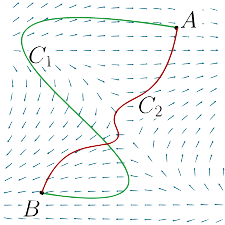
\includegraphics[width=.25\textwidth]{imagenes/img02-11.png}
		\caption*{\scriptsize{Campo conservativo: W depende solo de $A$ y $B$}\normalsize{.}}
		\end{figure}
\end{multicols}

\begin{multicols}{2}
\begin{figure}[H]
		\centering
		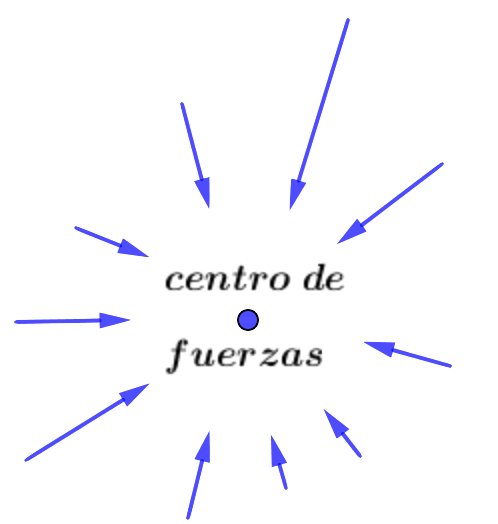
\includegraphics[width=.25\textwidth]{imagenes/img02-12.png}
		\caption*{\footnotesize{Campo central}\normalsize{.}}
		\end{figure}
Un caso particular de campo conservativo muy importante es el \emph{campo central:} cuando se deposita una magnitud activa en el campo aparecen sobre ella las fuerzas del campo que están dirigidas hacia el \emph{centro de fuerzas} y suelen ser \emph{inversamente proporcionales al cuadrado de la distancia} de la posición que ocupa la magnitud activa al el centro de fuerzas.
\end{multicols}

\vspace{2mm} \emph{\underline{Un campo de fuerzas central es necesariamente conservativo.}} Al ser central solo depende de la posición del centro de fuerzas y varía con la distancia (no necesariamente como $1/r^2$), veamos que es conservativo:

\vspace{2mm} Sea $M$, la magnitud activa del campo central $\vec E$, $\ \vec F=M \; \vec E= M \; \vec u_r \; \varphi(r)$, donde $\vec u_r=\dfrac {\vec r}{r}$ es un vector unitario que apunta al centro de fuerzas desde la posición que ocupe la magnitud activa y $\varphi(r)$ es la forma en que varía $\vec E$ con la distancia al centro de fuerzas.

\vspace{2mm}  Calculemos el trabajo necesario para desplazar la magnitud activa $M$ bajo la acción del campo central $\vec E$ desde un punto $A$ hasta otro $B$.
 
\vspace{2mm}  $\displaystyle W=\int_A^B \overrightarrow F \cdot \dd \vec r =\int_A^B M\; \varphi(r) \;\vec u_r \cdot \dd r= \int_A^B M\; \varphi(r) \; \dfrac {\vec r}{r} \cdot \dd r =(*) \int_A^B M\; \varphi(r) \; \dfrac {\cancel{r}\;\dd r}{\cancel{r}}=\int_A^B M\; \varphi(r)\; \dd r=(**)\eval{\Phi(r)}_{A}^B=\Phi(B)-\Phi(A)$
 
 \vspace{2mm}
 \textcolor{gris}{
 $(*)\quad \vec r\cdot \dd \vec r=r\;\dd r \cos 0^o=r\; \dd r $}
 
\textcolor{gris}{
 $(**)\quad \mathcal A\; \varphi(r)$ depende solo de $r$ y su primitiva será de la forma $\Phi(r)$ }

\vspace{2mm} Luego ``todo campo central es conservativo'' ya que el $W$ depende solo de las posiciones inicial $A$ y final $B$ y no del camino seguido. $\qquad \square$

\vspace{2mm} \textbf{Energia Potencial. Concepto de gradiente}

\vspace{2mm} Definición de energía potencial: \emph{El trabajo que realiza un campo de fuerza \underline{conservativo} al desplazar un cuerpo desde un punto $A$ hasta un punto $B$ es igual a la diferencia de energías potenciales existentes en los puntos $A$ y $B$.}

\begin{equation}
\label{Ener-poten}
W_{A\to B}=\int_A^B \vec F \cdot \dd \vec r = \mathcal E_p(A)- \mathcal E_p(B)\; \qquad \textcolor{gris}{(\vec F\; \text{conservativa})}	
\end{equation}

Esto que llamamos energía potencial $ \mathcal E_p$ es una función escalar característica del campo conservativo.

\vspace{2mm}
\rule{150pt}{0.4pt} 

\textbf{Otra definición de `campo conservativo':} 

\begin{multicols}{2}
$\,$

\emph{En un campo conservativo, el trabajo a lo largo de una trayectoria cerrada es cero.}
\begin{figure}[H]
		\centering
		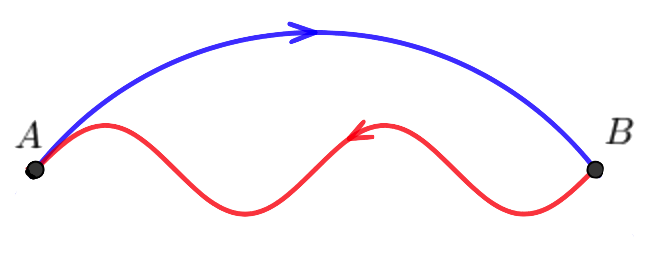
\includegraphics[width=.3\textwidth]{imagenes/img02-13.png}
		\end{figure}
\end{multicols}

$W_{A\to A}=W_{A\to B}+W_{B \to A}=\mathcal E_p(A)-\mathcal E_p(B) \;+ \; \mathcal E_p(B)-\mathcal E_p(A)=0$

$$ \text{Campo conservativo:}\qquad \oint \vec F \cdot \dd \vec r =0$$

\textcolor{gris}{$\oint$ representa a la integral curvilínea cerrada.}

\rule{150pt}{0.4pt} 

\vspace{2mm}
\begin{equation}
\int_A^B \vec F \cdot \dd \vec r = \mathcal E_p(A)- \mathcal E_p(B)=-\int_A^B\dd \mathcal E_p	
\end{equation}

\begin{multicols}{2}
$\dd r = \dd l$, en la dirección de movimiento

$\vec F\cdot \dd \vec r=F\; \dd l\; \cos \theta =-\dd \mathcal E_p $

$F \cos \theta=- \dfrac{\dd \mathcal E_p}{\dd l} \; \to \;\; \vec u_r\;F \cos \theta=-\vec u_r\; \dfrac{\dd \mathcal E_p}{\dd l}$
\begin{figure}[H]
		\centering
		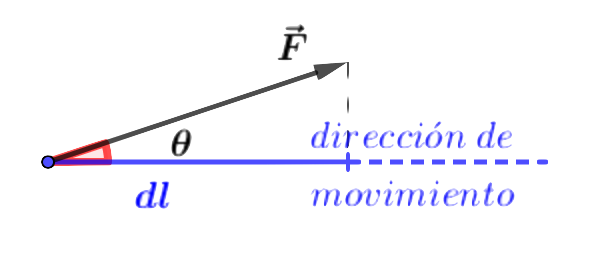
\includegraphics[width=.4\textwidth]{imagenes/img02-14.png}
		\end{figure}
\end{multicols}

\vspace{2mm}
$F\cos \theta$ es la componente de la fuerza en la dirección del movimiento, por ello, si conocemos $\mathcal E_p(x,y,z)$, podemos conocer la componente de $\overrightarrow F$ en cualquier dirección a partir de la cantidad $-\dd \mathcal E_p / \dd l$. Esto es lo que se llama \emph{derivada direccional} de $\mathcal E_p$. Cuando un vector es tal que su componente en una dirección determinada es igual a la derivada direccional de una función escalar en esa dirección, al vector se le llama \emph{gradiente} de la función escalar: $\vec F=-grad\;( \mathcal E_p)$

\vspace{2mm} Cuando estamos interesados en las componentes rectangulares de $\overrightarrow F$, la expresión $F \cos \theta$ es $F_x$, $F_y$ y $F_z$ y el desplazamiento $\dd l$ será $\dd x$, $\dd y$, y $\dd z$, de modo que:

\vspace{2mm} $\displaystyle F=\vec i\; F_x +\vec j\; F_y +\vec k\; F_z; \qquad F_x=- \pdv{\mathcal E_p}{x};\; F_y=- \pdv{\mathcal E_p}{y};\; F_z=- \pdv{\mathcal E_p}{z}$


\vspace{2mm}$\displaystyle \vec F=-\left[\;\vec i\;\;\pdv{\mathcal E_p}{x} + \vec j\;\;\pdv{\mathcal E_p}{y} + \vec k\;\;\pdv{\mathcal E_p}{z}\; \right]$

\vspace{2mm}
\begin{equation}
\displaystyle \vec F=- \left( \;\vec i\;\;\pdv{x} + \vec j\;\;\pdv{y} + \vec k\;\;\pdv{z}\; \right)\; \mathcal E_p
\end{equation}

\vspace{2mm}
Si llamamos `gradiente' al operador \emph{nabla}: $\displaystyle \grad= \vec i\;\;\pdv{x} + \vec j\;\;\pdv{y} + \vec k\;\;\pdv{z}$

\vspace{2mm}
\begin{equation}
\label{Ep-gradiente}
\vec F=-\overrightarrow{ \grad } \mathcal E_p	
\end{equation}

\vspace{2mm}
\emph{La energía potencial es característica de los campos conservativos.} 
En campos no conservativos no tiene sentido hablar de energía potencial.

\vspace{2mm}
$\displaystyle \pdv{F_x}{y}=-\pdv{\mathcal E_p}{y}{x} \quad = \quad -\pdv{\mathcal E_p}{x}{y}=\pdv{F_y}{x} \quad \to \quad \pdv{F_x}{y}-\pdv{F_y}{x}=0$ 

\vspace{2mm} Esto se cumple, por analogía, para las tres componentes:

\vspace{2mm} $\displaystyle \pdv{F_z}{y}-\pdv{F_y}{z}=0 \; \textcolor{gris}{\to\;  \vec i}\;;\quad \pdv{F_z}{x}-\pdv{F_x}{z}=0 \;\textcolor{gris}{\to\;  \vec j}\;;\quad \pdv{F_y}{x}-\pdv{F_x}{y}=0 \;\textcolor{gris}{\to\;  \vec k}$

\vspace{2mm} Y estas son las 3 condiciones que permiten definir matemáticamente a un campo conservativo: \emph{Un campo $\vec F$ es conservativo sus componentes satisfacen simultáneamente las tres ecuaciones anteriores.}

\vspace{2mm} Si lo escribimos vectorialmente:

\vspace{2mm} $\displaystyle \left( \pdv{F_z}{y}-\pdv{F_y}{z} \right) \;  \vec i+
\left( \pdv{F_z}{x}-\pdv{F_x}{z} \right) \;  \vec j+
\left( \pdv{F_y}{x}-\pdv{F_x}{y} \right) \;  \vec k\;$,

\vspace{2mm} que podemos escribir como:

\vspace{2mm} $\displaystyle \left| \begin{matrix} \vec i&\vec j&\vec k \\ \pdv{x}&\pdv{y}&\pdv{z} \\ F_x&F_y&F_z  \end{matrix} \right|=0 \to \overrightarrow{\grad } \times \vec F = 0$, si hacemos uso del operador nabla.

\vspace{2mm} Cuando el operador nabla actúa como producto vectorial sobre un vector se le llama \textbf{\emph{rotacional}}.


\vspace{2mm} $$\vec F \text{ es conservativo } \leftrightarrow \overrightarrow{\grad } \times \vec F = 0$$ 

\vspace{2mm} \emph{Un campo de fuerzas es conservativo si su rotacional es cero en todos los puntos.}

\vspace{2mm} \textcolor{gris}{Por ejemplo, el campo $\vec F=3x\vec i+5\vec j+7\vec k \to \overrightarrow{\grad } \times \vec F = \left| \begin{matrix} \vec i&\vec j&\vec k \\ \pdv{x}&\pdv{y}&\pdv{z} \\ 3x&5&7  \end{matrix} \right|=0$ y el campo es conservativo}.

\vspace{2mm} \textbf{Teorema de Stookes}: Un campo es conservativo si el trabajo para desplazar la masa activa de un punto $A$ a otro $B$ es independiente del camino elegido.

\begin{equation}
\label{Th-Stookes}
	\vec F \text{\;conservativo} \quad \leftrightarrow \quad  \overrightarrow{\grad } \times \vec F = 0 \quad \leftrightarrow \quad \oint \vec F \cdot \dd \vec r =0
\end{equation}

\vspace{2mm} -- La integral de curvilínea cerrada de $\vec F$ escalarmente por $\dd \vec r$ es cero.

\vspace{2mm} -- El rotacional del campo de fuerzas $\vec F$ es cero en todos los puntos del campo.

\vspace{2mm} Al ser $\vec F=- \overrightarrow{\grad} \mathcal E_p = - \overrightarrow{\grad} \mathcal (E_p+ Cte)$, pues $(Cte)'=0$, tenemos que \emph{la energía potencial es un valor funcional definida salvo una constante arbitraria (origen de energía potencial).} Esa constante no influye en los cálculos pues, al calcular la fuerza la constante desparecen al derivar y al calcular el trabajo, diferencia de energías potenciales, la constante desaparece al restar. Es usual, para campos eléctricos y gravitatorios, escoger esa constante de modo que se anule para puntos alejados de la partícula que crea en campo ($\mathcal E_p \to 0$ cuando $r\to \infty$).
 
 
\vspace{2mm} \emph{Tanto la energía cinética como la potencial dependen del sistema de referencia elegido.}

\rule{150pt}{0.4pt} 

En el ejemplo anterior, $\vec F = 3x\vec i + 5 \vec j+7\vec k=\displaystyle - \overrightarrow{\grad} \mathcal E_p$, es fácil obtener que el funcional energía potencial es $\mathcal E_p=3\frac{x^2}2+5y+7j+\mathcal K$, con $\mathcal K$ la constante arbitraria.

$\mathcal E_p(2,-3,1)=6-15+7=-2$, si deseamos que el origen de potencial este en el punto $(2,-3,1)$, definiremos la energía potencial como: $E_p=3\frac{x^2}2+5y+7j-2$.

\rule{150pt}{0.4pt} 


\vspace{2mm} \textbf{Significado físico-matemático del gradiente}
\label{potenciales-decrecientes}
\begin{multicols}{2}
$\, $

Supongamos una región del campo en que $\mathcal E_p(x,y,z)=cte$, matemáticamente esto es una \emph{superficie}.
\begin{figure}[H]
		\centering
		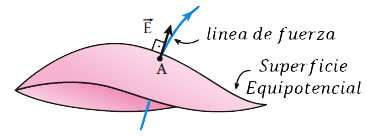
\includegraphics[width=.5\textwidth]{imagenes/img02-19.png}
		\end{figure}
\end{multicols}

\vspace{2mm} $\mathcal E_p(x,y,z)=cte \to - \overrightarrow{\grad} \mathcal E_p = 0 = \vec F \cdot \dd \vec r \to \left( \; \vec F \;\parallel \; \overrightarrow{\grad}  \mathcal E_p \; \right) \; \; \bot \; \; \dd \vec r$

\vspace{2mm} El vector $\vec F$ o el vector gradiente es \emph{perpendicular} a la superficie equipotencial.

\begin{multicols}{2}
\vspace{2mm} Sea $\vec u_R$ un vector unitario en la dirección en que actúa la fuerza sobre la magnitud activa. Como
$\vec F = \vec u_R \; F=- \vec u_R \; \dv{\mathcal E_p}{R}\;$
para que $F>0$, $\dv{\mathcal E_p}{R} <0$. La fuerza está orientada em el sentido de potenciales decrecientes: $\mathcal E_{p_2} < \mathcal E_{p_1} \to \dd \mathcal E_p < 0$

\vspace{2mm} El vector fuerza (y el vector gradiente de energía potencial) es perpendicular a las superficies equipotenciales en cada punto y está orientado hacia los potenciales decrecientes.

\begin{figure}[H]
		\centering
		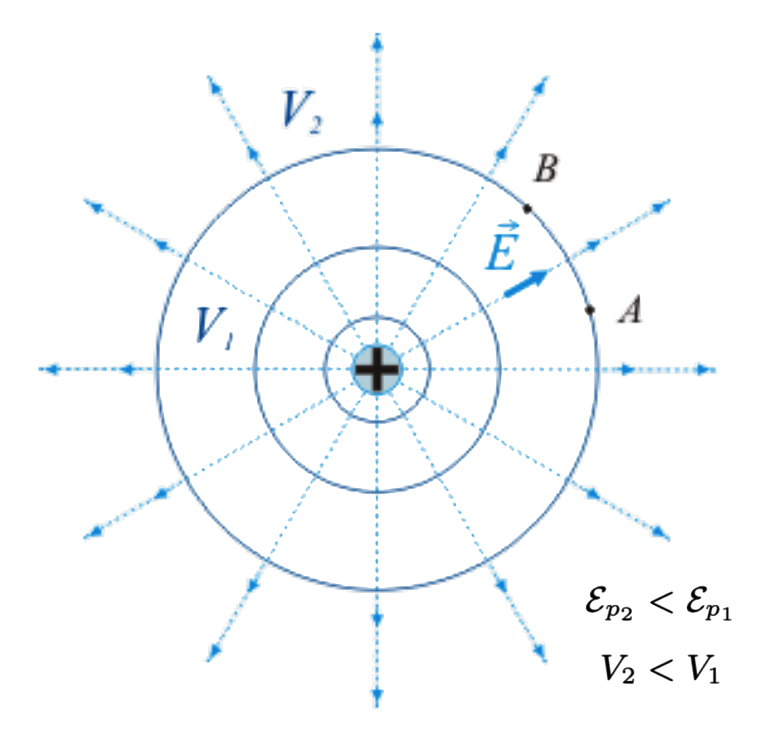
\includegraphics[width=.4\textwidth]{imagenes/img02-20.png}
		\end{figure}
\end{multicols}		

\begin{flushright}
\begin{scriptsize}
	\rule{250pt}{0.1pt}

\textcolor{gris}{`Física General', Ignacio Vallés, }\textcolor{teal}{{http://igvaori.github.es}} $\quad$
\end{scriptsize}	
\end{flushright}

 
\end{myexampleblock}
\end{small}	




\chapter{Ejemplo \emph{Euler-Lagrange}}
\label{capejemEE}

	\begin{tikzpicture}
	\fill [left color=red!50, right color=teal!50] (0,0) rectangle (6.5,.1);
	\fill [left color=teal!50, right color=blue!50] (6.5,0) rectangle (11.5,.1);
	\end{tikzpicture}
\vspace{1cm}

\begin{adjustwidth}{50pt}{50pt}
\begin{ejemplo}
	Vamos a ver la aplicación de las ecuaciones de \emph{Euler-Lagrange} a  un ejemplo de un sistema físico sin rozamiento, para encontrar las ecuaciones del movimiento.
\end{ejemplo}
\end{adjustwidth}

\vspace{0.5cm}

\begin{myblock}{Ecuaciones Euler-Lagrange}
\begin{large}
	\begin{equation}
	\dv{t} \left[ \pdv{ L }{\dot q_i} \right] \ - \ \pdv{L}{q_i} \ = \ 0	\, ; \quad i=1,2,\cdots n
	\end{equation}
\end{large}
\end{myblock}

\vspace{0.5cm}

\section{Ejemplo \emph{Euler-Lagrange}}
\label{T3ejem}


\begin{example}

\vspace{3mm} 
Una partícula de masa $M$ se mueve libremente sin rozamiento sobre el eje horizontal $X$. De ella cuelga una segunda partícula de masa $m$ suspendida de una barra rígida de masa despreciable y longitud $b$ a la que se la separa un ángulo $\theta$ de la vertical y se la deja oscilar libremente (también sin rozamiento). 	
	
	Encontrar las ecuaciones del movimiento.
	
	\begin{figure}[H]
		\centering
		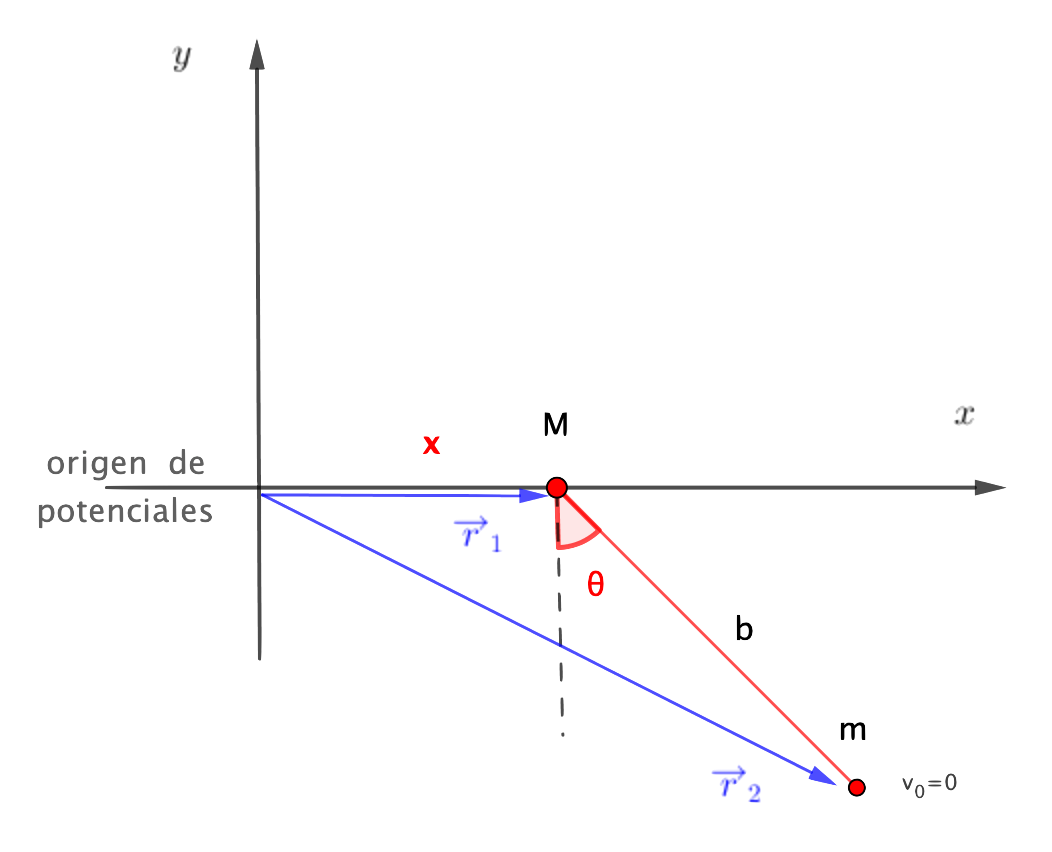
\includegraphics[width=.75\textwidth]{imagenes/img03-01.png}
		\end{figure}	
\end{example}

Buscamos las coordenadas generalizadas que, una vez fijadas, determinarán la configuración del sistema: $\boldsymbol x$ y $\boldsymbol \theta$. Estas variables proporcionarán las ecuaciones del mevimiento del sistema $M, m, b$.

$x \text{ y } \theta$ son nuestras $q_1 \text{ y } q_2$, pero vamos a mantener la notación $x,\ \theta$ por sencillez.

Las posiciones de las partículas viene dadas por:

$\overrightarrow r_1 = (x,0)\ ; \qquad \overrightarrow r_2=\overrightarrow r_1 + \overrightarrow b = \overrightarrow r_1 + (b\sin \theta, -b ºcos \theta)$

Calculemos la energía cinética:

$T=T_1+T_2=\dfrac 1 2 ; v_1^2 + \dfrac 1 2 m v_2^2$

$\overrightarrow v_1= \dot{\ \overrightarrow r_1}=(\dot x, 0)$
$ \quad \longrightarrow \quad$
$v_1^2=\overrightarrow v_1 \cdot \overrightarrow v_1 = (\dot x,0) \cdot (\dot x, 0)={\dot x}^2$

$\overrightarrow v_2=\dot{\ \overrightarrow r_2}= \dot{\ \overrightarrow r_1} + \dot{\ \overrightarrow b} = (\dot x,0) + b (\cos \theta \ \dot \theta, \sin \theta \ \dot \theta) = \overrightarrow A + \overrightarrow B \to$

$\longrightarrow \  v_2^2=\overrightarrow v_2 \cdot \overrightarrow v_2 =
A^2+2AB+B^2={\dot x}^2+2\ b \ \dot \theta \ \dot x \cos \theta + b^2 \ {\dot \theta}^2$

$\boldsymbol T=\dfrac 12 M \dot x ^2 +\dfrac 12 m (\dot x^2 + 2 b \dot \theta \dot x \cos \theta + b^2 \dot \theta^2)=
\boldsymbol{\dfrac 1 2 \ (M+m)\ \dot x^2 + \dfrac 1 2 \ m \ b^2 \ \dot \theta^2 +m \ b \ \dot \theta \ \dot x \cos \theta}$

Calculemos, ahora la energía potencial:

$\boldsymbol V=V_m+V_m=0+mg(-b\cos \theta)=\boldsymbol{-b\ m \ g  \cos \theta}$

Podemos formar ya el \emph{lagrangiano} del sistema:

\begin{small}
\begin{equation}
\label{T3lagran}
\boxed{ \ 
\boldsymbol{ L=T-V= } \boldsymbol{\dfrac 1 2 \ (M+m)\ \dot x^2 + \dfrac 1 2 \ m \ b^2 \ \dot \theta^2 +m \ b \ \dot \theta \ \dot x \cos \theta + m\ g \ b \cos \theta}
\ }
\end{equation}
\end{small}

Tenemos una ecuación de Euler-Lagrange para cada una de las dos coordenadas generalizadas del sistema: $\boldsymbol x$ y $\boldsymbol \theta$

$$ \subrayado{ \ 
 \displaystyle
\dv{t} \left[ \pdv{ L }{\dot q_i} \right] \ - \ \pdv{L}{q_i} \ = \ 0	
\quad \to \quad
\begin{cases}
\displaystyle \ \ \dv{t} \left[ \pdv{ L }{\dot x} \right] \ - \ \pdv{L}{x} \ = \ 0	
\\ \\
\displaystyle \ \ \dv{t} \left[ \pdv{ L }{\dot \theta} \right] \ - \ \pdv{L}{\theta} \ = \ 0		
\end{cases}
\ }$$

\vspace{0.5cm}
\subsection{Ecuación de movimiento para $\boldsymbol x$}
\begin{tikzpicture}
	\fill [left color=red!50, right color=teal!50] (0,0) rectangle (3.5,.01);
	\fill [left color=teal!50, right color=blue!50] (3.5,0) rectangle (7.5,.01);
	\end{tikzpicture}
\vspace{0.5cm}

$$\displaystyle \ \ \dv{t} \left[ \pdv{ L }{\dot x} \right] \ - \ \pdv{L}{x} \ = \ 0	$$

$\displaystyle \dv{t} \left[ \pdv {L} {\dot x} \right]=
\dv{t} \left[  \dfrac{1}{\cancel{2}} (M+m) \cancel{2} \dot x +   m b \dot \theta \cos \theta \right]=
(M+m)\ \ddot x +m\ b \ [\ddot \theta \cos \theta - \dot \theta^2 \sin \theta]$

$\displaystyle \pdv{L}{x}=0$

\begin{flushright}
	$\Rightarrow \quad \boldsymbol{(M+m)\ \ddot x + m\ b [\ddot \theta \cos \theta -\dot \theta^2 \sin \theta]=0}$
\end{flushright}

En esta ocasión,
$L=L(\dot q) \neq L(q) \to$ tenemos \emph{coordenadas cíclicas} y ocurre que $\displaystyle \pdv{L}{x}=0$ por lo que las ecuaciones de Euler-Lagrange se reducen a $\displaystyle \dv{t} \left( \pdv{L}{\dot q} \right) =0$, lo que asegura que $\displaystyle \pdv{L}{\dot q}=cte$.
\textcolor{gris}{A lo largo del curso veremos que esto tiene que ver con \emph{leyes de conservación}}.


Luego, la ecuación de movimiento para la variable $\boldsymbol x$ es:

\begin{equation}
\boxed{ \ 
\boldsymbol{
(M+m)\ \dot x + m\ b\ \dot \theta \cos \theta \ = \
\textcolor{gris}{cte}
\ = \ K 
} \ }
\end{equation}




\vspace{0.5cm}
\subsection{Ecuación de movimiento para $\boldsymbol \theta$}
\begin{tikzpicture}
	\fill [left color=red!50, right color=teal!50] (0,0) rectangle (3.5,.01);
	\fill [left color=teal!50, right color=blue!50] (3.5,0) rectangle (7.5,.01);
	\end{tikzpicture}
\vspace{0.5cm}

$$\displaystyle \ \ \dv{t} \left[ \pdv{ L }{\dot \theta} \right] \ - \ \pdv{L}{\theta} \ = \ 0	$$


$\displaystyle \dv{t} \left[ mb^2 \dot \theta + m b \dot x \cos \theta \right]= m\ b^2 \ \ddot \theta^2 + m \ b \ ( \ddot x \cos \theta - \dot x \ \dot \theta \sin \theta )$

$\displaystyle \pdv{L}{\theta}=-m\ b \ \dot \theta \ \dot x \sin \theta - m \ g \ b \sin \theta$

$\Rightarrow mb^2\ddot \theta + mb(\ddot x \cos \theta - \cancel{\dot x \dot \theta \sin \theta}) = -\cancel{mb\dot \theta \dot x \sin \theta} -mgb\sin \theta$

$ \cancel{m} b^2 \ddot \theta + \cancel{m} b \ddot x \cos \theta =-\cancel{m} gb \sin \theta$

$\ddot \theta + \dfrac 1 b \ddot x \cos \theta = - \dfrac g b \sin \theta$

\begin{flushright}
	$\Rightarrow \quad \boldsymbol{
	\ddot \theta \ = \  -\dfrac{\ddot x}{b} \ \cos \theta \ - \ \dfrac g b \ \sin \theta
	}$
\end{flushright}

La ecuación de movimiento para la variable $\boldsymbol \theta$ es:

\begin{equation}
	\boxed{ \ 
	\boldsymbol{
		\ddot \theta \ = \  -\dfrac{\ddot x}{b} \ \cos \theta \ - \ \dfrac g b \ \sin \theta
	} \ }
\end{equation}



\vspace{0.5cm}
\subsection{Ecuaciones de movimiento}
\begin{tikzpicture}
	\fill [left color=red!50, right color=teal!50] (0,0) rectangle (3.5,.01);
	\fill [left color=teal!50, right color=blue!50] (3.5,0) rectangle (7.5,.01);
	\end{tikzpicture}
\vspace{0.5cm}


\begin{myalertblock}{Ecuaciones del movimiento}

\begin{equation}
\begin{cases}
	\quad \boldsymbol{(M+m)\ \dot x + m\ b\ \dot \theta \cos \theta \ = \ K } \\ \\
	\quad \boldsymbol{\ddot \theta \ = \  -\dfrac{\ddot x}{b} \ \cos \theta \ - \ \dfrac g b \ \sin \theta}
\end{cases}
\end{equation}
\end{myalertblock}

\vspace{5mm}
Resolver este sistema de ecuaciones diferenciales \emph{acopladas} solo puede hacerse numéricamente (con Mathlab, por ejemplo).

Para ello, determinemos antes la constante K imponiendo condiciones iniciales: $t=0 \to \dot x=0;\ \dot \theta=0$. 

Con esto, $\ (M+m)\ 0 + m\ b\ 0\cos \theta = K \ \to \boldsymbol{K=0}$

En la siguiente figura se observan diferentes imágenes del movimiento recreado con Mathlab, se observa que mientras la masa $m$ oscila, también se desplaza en el eje $X$ en sentido contrario a como lo hace $M$.


\vspace{5mm}
\begin{figure}[H]
		\centering
		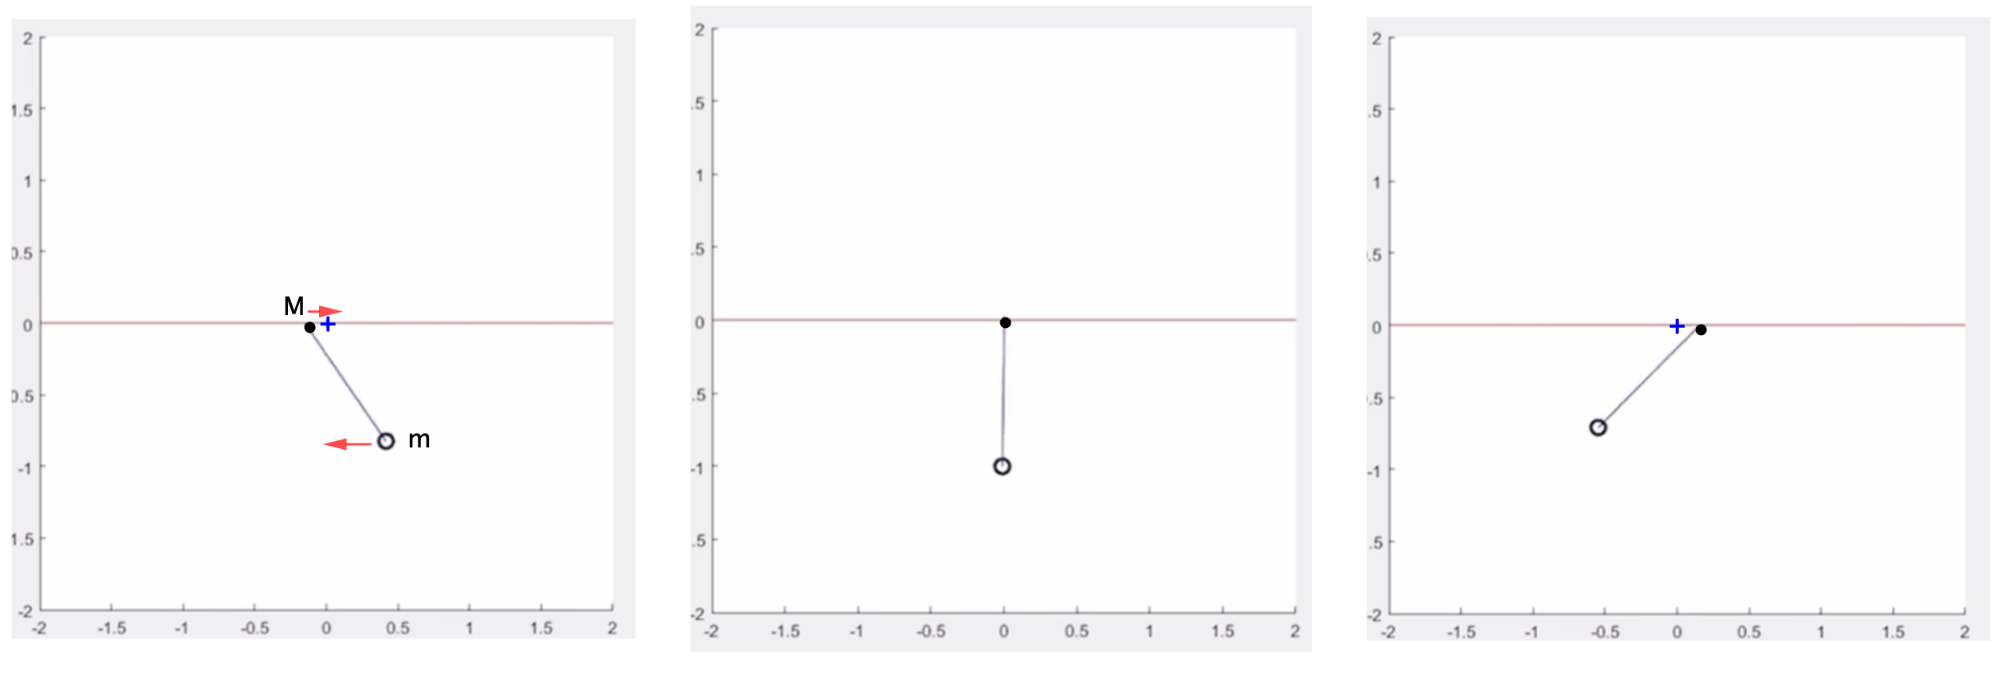
\includegraphics[width=0.9\textwidth]{imagenes/img03-02.png}
		\end{figure}


\vspace{-0.5cm}
\begin{myexampleblock}{Partícula libre}
	\begin{multicols}{2}
		\begin{figure}[H]
		\centering
		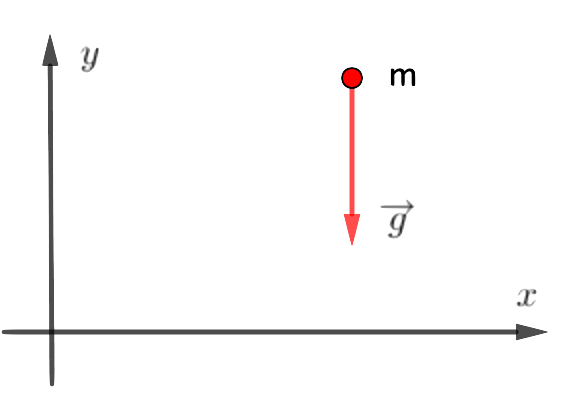
\includegraphics[width=.4\textwidth]{imagenes/img03-03.png}
		\end{figure}
		$q_1=x$; $q_2=y$
		
		\vspace{2mm} $T=\dfrac 1 2 m(\dot x^2 + \dot y^2)$
		
		\vspace{2mm} $V=-mgy$
		
		\vspace{4mm} $\boldsymbol{ L=\dfrac 1 2 m(\dot x^2 + \dot y^2)-mgy }$
	\end{multicols}
	
\vspace{3mm} $\triangleright \ \ \displaystyle \pdv{L}{\dot x}=\dfrac 1 2 m 2 \dot x = m\dot x;\quad \dv{t} \left[ \pdv{L}{\dot x}\right] = \dv{t} \left[ m \dot x \right]=\ddot x$

\vspace{3mm} $\displaystyle \pdv{L}{x} =0 \quad \Rightarrow \quad E-L:\quad \boldsymbol{ m\dddot x= 0}$

\vspace{3mm} $\triangleright \ \ \displaystyle \pdv{L}{\dot y}=\dfrac 1 2 m 2 \dot y = m\dot y;\quad \dv{t} \left[ \pdv{L}{\dot y}\right] = \dv{t} \left[ m \dot y \right]=\ddot y$

\vspace{3mm} $\displaystyle \pdv{L}{y} =-mg \quad \Rightarrow \quad E-L:\quad \boldsymbol{ m\dddot y= -mg}$

\vspace{4mm}Las ecuaciones del movimiento son \textcolor{gris}{(MRUA, tiro parabólico)}:

\begin{equation*}
	\begin{array}{l}
	\ddot x=0 \quad  \quad \to \qquad x(t)=x_0+v_{x_0} t
	\\
	\ddot y=-q \quad \to \qquad y(t)=y_0+v_{y_0} t - \dfrac 1 2 g t^2  	
	\end{array}
\end{equation*}


\end{myexampleblock}

%\vspace{0.5cm}
\begin{myexampleblock}{Péndulo simple}
\begin{multicols}{2}
	\begin{figure}[H]
		\centering
		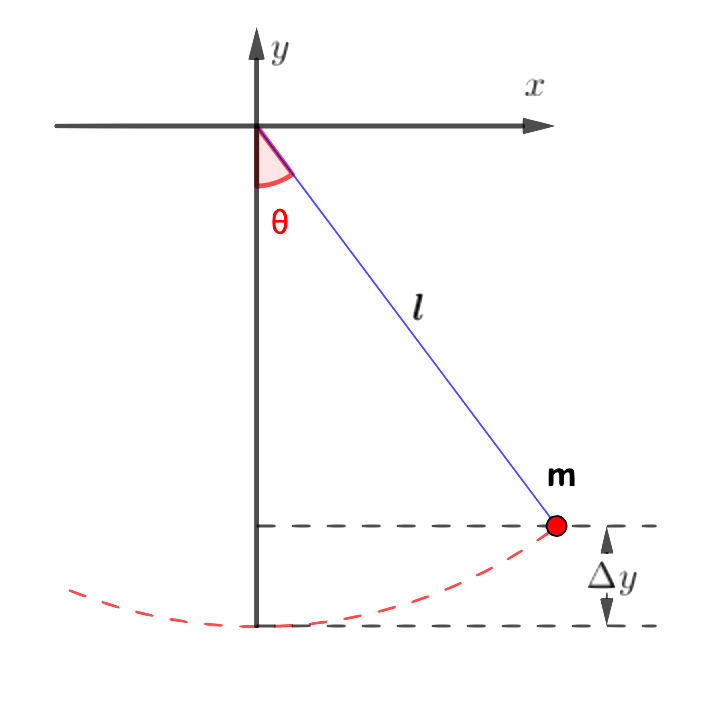
\includegraphics[width=.35\textwidth]{imagenes/img03-04.png}
		\end{figure}
		\vspace{2mm} Posición: $\ x=l\sin \theta; \ \ y=-l\cos \theta$
		
		\vspace{2mm} Velocidad: $\ \dot x=l \dot \theta \cos \theta; \ \ \dot y=l\dot \theta \sin \theta$
		
		\vspace{2mm} Solo 1 coordenada generalizada: $\ \boldsymbol \theta$
		
		\vspace{2mm} Energía cinética: 
		
		$\qquad T = \dfrac 1 2 m (\dot x^2+\dot y^2)= \dfrac 1 2 m l^2 \dot \theta ^2$
		
		\vspace{3mm} Energía potencial: 
		
		$\qquad V=mg\Delta y= mgl(1-\cos \theta)$	
\end{multicols}

\vspace{3mm} \textbf{Lagrangiano}: $\ L=T-V=\dfrac 1 2 ml^2\dot \theta^2 -mgl(1-\cos \theta)$
	
\vspace{3mm}\textbf{Ecuaciones de Euler-Lagrange}:

\vspace{2mm} $\displaystyle \pdv{L}{\dot \theta}=ml^2 \dot \theta; \ \ \dv{t}\left( \pdv{L}{\dot \theta} \right)=ml\ddot \theta; \quad \pdv{L}{\theta}=-mgl \sin \theta$

\vspace{2mm} $\displaystyle \dv{t}\left( \pdv{L}{\dot \theta} \right)-\pdv{ }{q}=0 \qquad \longrightarrow \qquad  \boldsymbol{ \boxed{ \ddot \theta = -\dfrac g l \sin \theta = -\omega_0^2 \sin \theta \ } } $

\vspace{2mm}Hemos llamado $\omega=\sqrt{\dfrac g l}$

\vspace{3mm} Para pequeñas oscilaciones, $\sin \theta \approx \theta$, tenemos $\boldsymbol{\ddot \theta=-\omega_0^2 \theta}$, integrando, $\boldsymbol{\theta(t)=A \sin(\omega_o t+\varphi)}$, siendo $A=\theta_{max}$ la amplitud y $\varphi$ el ángulo de fase; $\omega_0$ es la frecuencia. 
\end{myexampleblock}



	


\vspace{0.3cm}
\begin{myexampleblock}{Máquina de Atwood}
	\begin{multicols}{2}
		\begin{figure}[H]
		\centering
		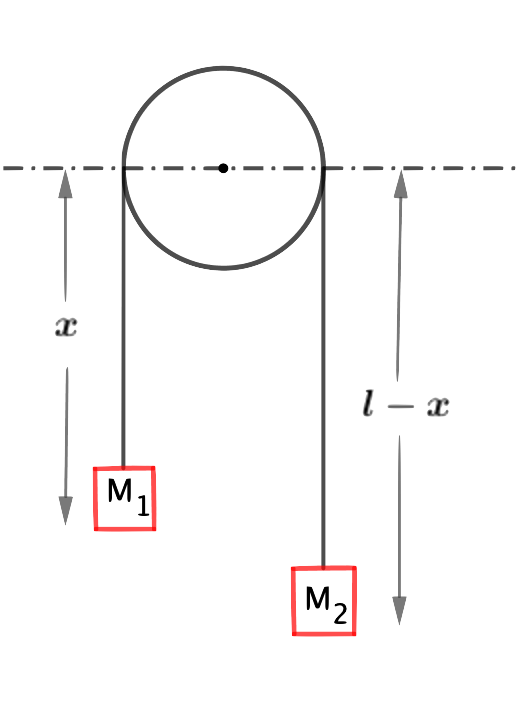
\includegraphics[width=.35\textwidth]{imagenes/img03-05.png}
		\end{figure}
	La polea se supone sin masa ni rozamiento y la cuerda rígida y sin masa. Solo hay una coordenada independiente, $\boldsymbol x$, dada la posición de una masa, la otra queda determinada al saber que la longitud total de la cuerda que las une vale $\boldsymbol l$.
	
	\vspace{5mm} $T=\dfrac 1 2 (M_1+M_2) \dot x ^2$
	
	\vspace{2mm} $V=-M_1gx - M_2g(l-x)$
	
	
	\vspace{5mm} $L=T-V= $
	
	$=\dfrac 1 2 (M_1+M_2)\dot x^2 +M_1gx +M_2g(l-x)$
	\end{multicols}

\vspace{3mm} $\displaystyle \pdv{L}{\dot x}=(M_1+M_2) \dot x \quad \to \quad \dv{t} \left[ \pdv{L}{\dot x} \right]=(M_1+M_2) \ddot x$

\vspace{3mm} $\displaystyle \pdv{L}{x}=(M_1-M_2)g \quad \longrightarrow \qquad \boldsymbol{(M_1+M_2) \ \ddot x\ = \ (M_1-M_2) \ g}$

\vspace{5mm} La ecuación del movimiento es: $ \quad \boldsymbol{ 
\boxed{ 
\ \ddot x \ = \ \dfrac{M_1-M_2}{M_1+M_2}\ g 
\ }
}$

\vspace{5mm} En las ecuaciones de Euler-Lagrange no aparecen las fuerzas de ligadura, motivo por el que no ha. aparecido para nada la \emph{tensión} de la cuerda, habría que hallarla por otro método (Newton).
\end{myexampleblock}



\chapter{Ejemplo \emph{Euler-Lagrange} con Fricción}
\vspace{0.5cm}


\begin{adjustwidth}{50pt}{50pt}
\begin{ejemplo}
	En esta ocasión, vamos a ver la aplicación de las ecuaciones de \emph{Euler-Lagrange} a  un ejemplo de un sistema físico con rozamiento (proporcional a la velocidad), para encontrar las ecuaciones del movimiento.
\end{ejemplo}
\end{adjustwidth}

\vspace{0.5cm}

\section{Ecuaciones de \emph{Euler-Lagrange} con fricción}
\begin{tikzpicture}
	\fill [left color=red!50, right color=teal!50] (0,0) rectangle (6.5,.1);
	\fill [left color=teal!50, right color=blue!50] (6.5,0) rectangle (11.5,.1);
	\end{tikzpicture}

\vspace{1cm}



Vimos, en capítulo \ref{CapEEL}, las ecuaciones de Euler-Lagrange,

\begin{equation}
\boxed{ \ 
\dv{t} \left( \pdv{T}{\dot q} \right) \ - \ \pdv{T}{q} \ = \ Q \ = \ \overrightarrow F \cdot \pdv{\vec r}{q}	
\ }
\tag{\ref{T2PDD7}}
\end{equation}



Si consideramos que, además de fuerzas conservativas también va a haber fricción, $\ F=F^{Cons}+F^{Fric} \, , \ $ en $\ Q \ $ habrá dos términos: 

--- el correspondiente a las fuerzas conservativas, al provenir del gradiente de un potencial $\ V \ $escalar pasa a la izquierda y, junto con la energía cinética $\ T \ $ forman el lagrangiano $ \ L \ $ de las ecuaciones de Euler-Lagrange para el caso conservativo 

\begin{equation}
\boxed{
\dv{t} \left[ \pdv{ L }{\dot q} \right] \ - \ \pdv{L}{q} \ = \ 0	
\ } 
\tag{\ref{T2EEL1C}}
\end{equation}

--- el término de las fuerzas de fricción se queda en el miembro de la derecha y las \textbf{ecuaciones de Euler-Lagrange ante fuerzas conservativas y de  fricción} toman el siguiente aspecto:

\vspace{0.5cm}

\begin{large}
\begin{myblock}{\begin{normalsize}Ecuaciones de Euler-Lagrange ante fuerzas conservativas y de  fricción\end{normalsize}}
\begin{equation}
\label{T4EEF1}
\boldsymbol{ \
\dv{t} \left[ \pdv{ L }{\dot q} \right] \ - \ \pdv{L}{q} \ = \ Q_j^{Fric} \ = \ \sum_{i=1}^N \overrightarrow F_i^{Fric} \cdot \pdv{\overrightarrow r_i}{q_j}	
\ } 
\end{equation}	
\end{myblock}
\end{large}

\vspace{1cm}
\subsection{Ejemplo \emph{Euler-Lagrange} con fricción - 1}
\label{T4SecELF}
\begin{tikzpicture}
	\fill [left color=red!50, right color=teal!50] (0,0) rectangle (3.5,.01);
	\fill [left color=teal!50, right color=blue!50] (3.5,0) rectangle (7.5,.01);
	\end{tikzpicture}
\vspace{0.5cm}


\begin{example}
.	Una partícula de masa $M$ se encuentra en reposo en un punto sobre el eje $X$ (basta con suponer $M=\infty$). De ella cuelga una segunda partícula de masa $m$ suspendida de una barra rígida de masa despreciable y longitud $b$ a la que se la separa un ángulo $\theta$ de la vertical y se la deja oscilar libremente, pero se encuentra sometida a una fuerza de rozamiento $F$ proporcional a la velocidad. 	
	
	\vspace{2mm} Encontrar las ecuaciones del movimiento.

	\begin{figure}[H]
		\centering
		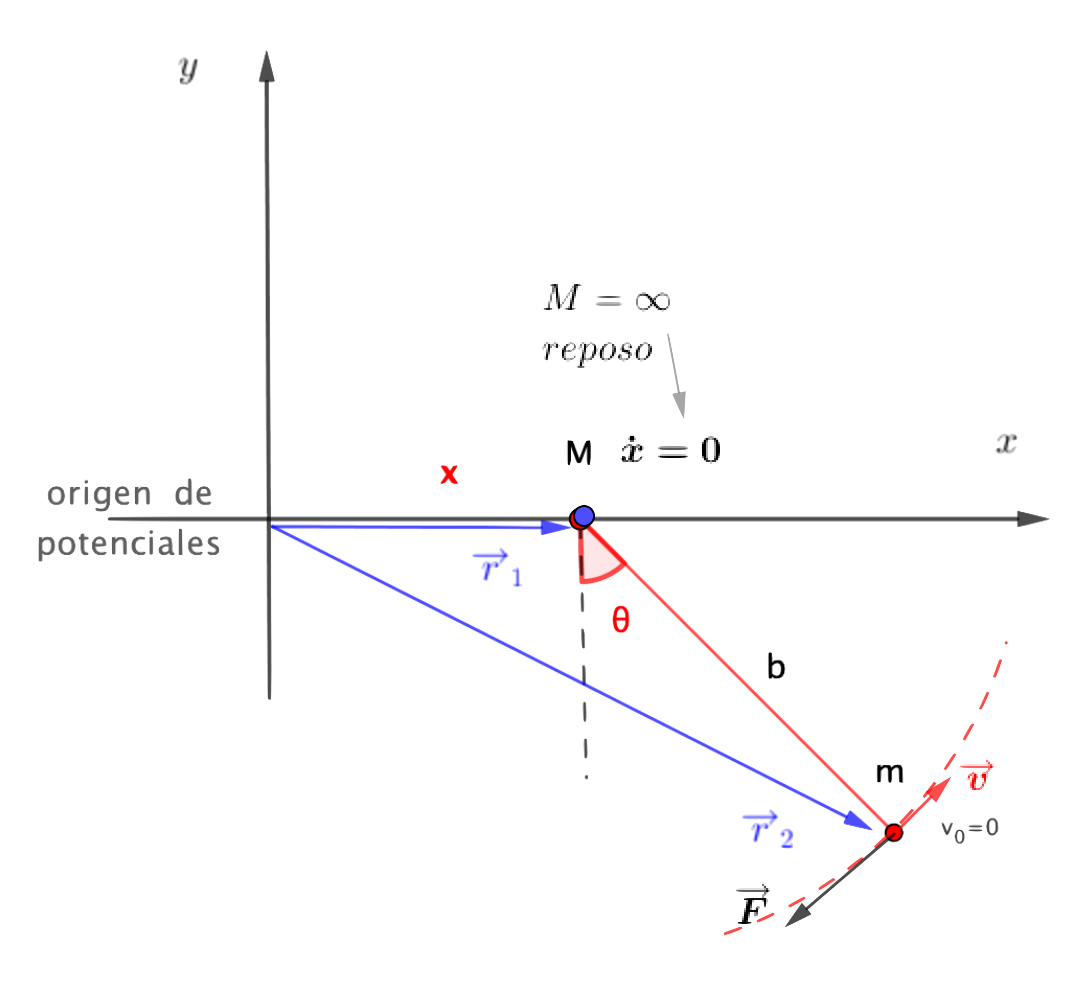
\includegraphics[width=.5\textwidth]{imagenes/img04-01.png}
		\end{figure}	
\end{example}

El ejemplo es el mismo que en el tema anterior (sección \ref{T3ejem}), por lo que el lagangiano será el mismo, pero teniendo en cuenta que la partícula de masa $M$ permanece en reposo, $\boldsymbol{\dot x=0}$,  particularizando ese resultado:

%\begin{small}
\begin{equation}
\tag{\ref{T3lagran}} 
 L=T-V=  
\cancelto{0}{ \dfrac 1 2 \ (M+m)\ \dot x^2 } + 
 \dfrac 1 2 \ m \ b^2 \ \dot \theta^2 +
 \cancelto{0}{ m \ b \ \dot \theta \ \dot x \cos \theta }+
 m\ g \ b \cos \theta 
\end{equation}
%\end{small}

El lagrangiano, en este caso, es:

\begin{equation}
\label{T4lagran-ejem1}
\boldsymbol{ 
 L\ = \ T-V \ = \  \dfrac 1 2 \ m \ b^2 \ \dot \theta^2  \ + \  m\ g \ b \cos \theta 
 }
\end{equation}

La fuerza de fricción (opuesta al movimiento) a la que se encuentra sometida $m$ es proporcional a la velocidad a la que ésta se mueve: $\ \overrightarrow F = - k \ \overrightarrow v$, es lo típico en el caso de movimiento es el seno de fluidos.

Calculamos la \emph{fuerza de fricción generalizada}, $Q^F$. Ahora solo tenemos una \emph{coordenada generalizada}, $\theta$.
$\quad \boldsymbol{ \displaystyle Q^F \ = \ \overrightarrow F \cdot \pdv{\overrightarrow r}{\theta} }$

Usando resultados que ya obtuvimos en el tema \ref{capejemEE}, en la sección \ref{T3ejem}, el vector de posición de las partícula $m$ es:

$\overrightarrow r = \overrightarrow r_2=\overrightarrow r_1+\overrightarrow b= (x,0)+(b\sin \theta,-b \cos \theta)=(x+b\sin \theta,-b \cos \theta)$

Derivando, $\quad \displaystyle \pdv{\overrightarrow r}{\theta}=b(\cos \theta, \sin \theta)$

Por lo que, $\quad \displaystyle Q^F=-K \overrightarrow v \cdot b (\cos \theta, \sin \theta)$

Veamos quién es $\overrightarrow v\, , \qquad \displaystyle \overrightarrow v=\dv{\overrightarrow r}{t}=(b \cos \theta \ \dot \theta, b \sin \theta \ \dot \theta)=b\ \dot \theta \ (\cos \theta, \sin \theta)$

Luego: $\quad \boldsymbol{ Q^F}=-kb\ \dot \theta \cdot b \ (\cos \theta, \sin \theta) =\boldsymbol{ -k\ b^2 \ \dot \theta }$

Llevando este resultado a las ecuaciones de Euler-Lagrange con fricción, ec \ref{T4EEF1}, y teniendo en cuenta cual es nuestro lagrangiano (ec. \ref{T4lagran-ejem1}),

$\begin{cases}
\ \ \displaystyle \dv{t} \left[ \pdv{L}{\dot \theta} \right] = \dv{t} [mb^2 \dot \theta]= m\ b^2 \ \ddot \theta 
\\ \\
\ \ \displaystyle \pdv{L}{\theta}=-mgb \sin \theta	
\end{cases} \quad \Rightarrow \quad m \ b^2\ \ddot \theta \ + \ m\ g\ b \ \sin \theta \ =\  -k\ b^2\ \dot \theta$

Pasando todo a la izquierda y dividiendo por $mb^2$,

\begin{equation}
\label{T4ecmonejem1}
\subrayado{ \ \boxed{ \ 	
\ddot \theta \ + \ \dfrac k m \ \dot \theta \ + \ \dfrac g b \ \sin \theta \ = \ 0 
\ } \ }
\end{equation}

Ecuaciones del movimiento. La dificultad para la resolución de esta ecuación diferencial estriba en la presencia del $\sin \theta$, pero podemos utilizar la \textbf{aproximación típica de ángulos pequeños}, $\ \ \boldsymbol{\theta << 1 \ \to \ \sin \theta \approx \theta}$. Con esto,

\begin{equation}
\label{T4ecmonejem1aprox}
\subrayado{ \ \boxed{ \ 	
\ddot \theta \ + \ \dfrac k m \ \dot \theta \ + \ \dfrac g b \  \theta \ = \ 0 
\ } \ }
\end{equation}

que es una EDO 2$^o$ orden lineal con coeficientes constantes homogénea, se puede resolver analíticamente. El resultado, ya conocido, es una oscilación que se va amortiguando con el tiempo.\footnote{ver al final del capítulo}

\begin{figure}[H]
		\centering
		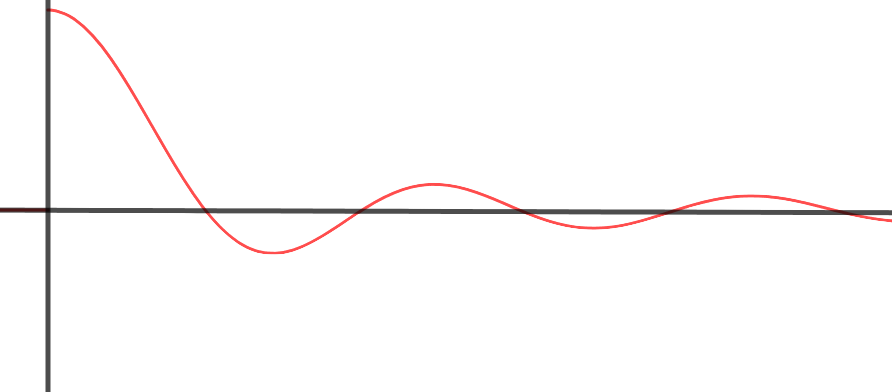
\includegraphics[width=.45\textwidth]{imagenes/img04-02.png}
		\end{figure}


\vspace{0.5cm}
\subsection{Ejemplo \emph{Euler-Lagrange} con fricción - 2}
\begin{tikzpicture}
	\fill [left color=red!50, right color=teal!50] (0,0) rectangle (3.5,.01);
	\fill [left color=teal!50, right color=blue!50] (3.5,0) rectangle (7.5,.01);
	\end{tikzpicture}
%\vspace{0.5cm}

Supongamos ahora que $M$ también se puede mover y que también está sometida a una fuerza de fricción.

\vspace{0.5cm}
\begin{example}

\begin{multicols}{2}

	Una partícula de masa $M$ se mueve con rozamiento (proporcional a la velocidad) sobre el eje horizontal $X$. De ella cuelga una segunda partícula de masa $m$ suspendida de una barra rígida de masa despreciable y longitud $b$ a la que se la separa un ángulo $\theta$ de la vertical y se la deja oscilar pero también está sometida a un rozamiento proporcional a la velocidad con s¡que se mueve. 	
	
	\vspace{2mm} Encontrar las ecuaciones del movimiento.

	\begin{figure}[H]
		\centering
		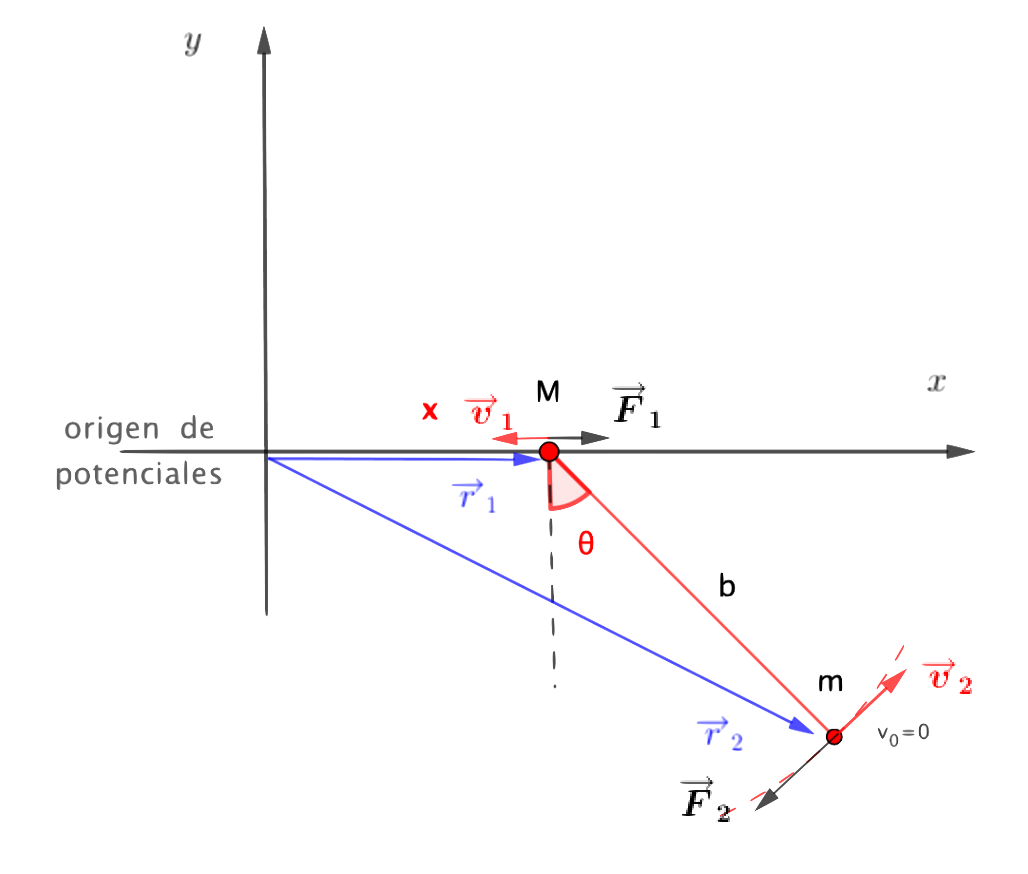
\includegraphics[width=.5\textwidth]{imagenes/img04-03.png}
		\end{figure}
\end{multicols}	
\end{example}

\vspace{0.5 cm}
\rule{200pt}{0.1pt}

Recuperamos los resultados obtenidos en el ejemplo del tema \ref{capejemEE}, en la sección \ref{T3ejem}, que siguen siendo válidos:

$ 
 L=T-V=  
 \dfrac 1 2 \ (M+m)\ \dot x^2  + 
 \dfrac 1 2 \ m \ b^2 \ \dot \theta^2 +
 m \ b \ \dot \theta \ \dot x \cos \theta +
 m\ g \ b \cos \theta 
$

$\begin{cases}
\ \overrightarrow r_1= (x,0) \\
\ \overrightarrow r_2=(x+b\sin \theta, -b\cos \theta	
\end{cases};
\quad
\begin{cases}
\ \overrightarrow v_1=(\dot x, 0) \\
\ \overrightarrow v_2=(\dot x + b \dot \theta \cos \theta, b \dot \theta \sin \theta)	
\end{cases}$

\begin{flushright}
\rule{200pt}{0.1pt}	
\end{flushright}

Calculemos, para más tarde, las siguientes derivadas:

$\displaystyle \pdv{\overrightarrow r_1}{x}=(1,0)\, ; \qquad \pdv{\overrightarrow r_2}{x}=(1,0)$

$\displaystyle \pdv{\overrightarrow r_1}{\theta}=(0,0)\, ; \qquad \pdv{\overrightarrow r_2}{\theta}=(b\cos \theta, b \sin \theta))$

\vspace{0.5cm}
Ahora, al aplicar las ecuaciones de Euler-Lagrange al caso en que haya fricción (ec. \ref{T4EEF1}), el miembro de la izquierda es el mismo que en el ejemplo de la sección \ref{T3ejem} del tema \ref{capejemEE} y, en el miembro de la derecha, tenemos que calcular las fuerzas generalizadas $Q^F_j$ debidas a las fuerzas de fricción $F_1$ que actúa sobre la partícula de masa $M$ y $F_2$ sobre $m$:

$\overrightarrow F_1 \ = \ - k_1\ \overrightarrow v_1 \, ; \qquad 
\overrightarrow F_2 \ = \ - k_2 \ \overrightarrow v_2$

Como hay dos coordenadas generalizadas, $q_1=\dot x \text{ y } q_2=\theta$, tendremos dos fuerzas generalizadas asociadas, $Q_x \text{ y } Q_{\theta}$

$\boxed{ \Rightarrow \  \ \boldsymbol {Q_x} \, : \ }$
$\qquad$
$Q_x=\displaystyle \sum_{i=1}^{2} \overrightarrow F_i \cdot \pdv{\overrightarrow r_i}{x} = 
\overrightarrow F_1 \cdot \pdv{\overrightarrow r_1}{x}+
\overrightarrow F_2 \cdot \pdv{\overrightarrow r_2}{x}$

$Q_x=-k_1\overrightarrow v_1 \cdot (1,0) - k_2 \overrightarrow v_2 (1,0)=-(k_1\overrightarrow v_1+k_2 \overrightarrow v_2) \cdot (1,0)=$

$Q_x=-[k_1(\dot x,0)+k_2(\dot x+b\dot \theta \cos \theta, b \dot \theta \sin \theta)]\cdot (1,0)=-k_1 \dot x - k_2(\dot x+b\dot \theta \cos \theta)$


\begin{equation}
Q_x \ = \ -(k_1+k_2) \ \dot x \ - \  k_2 \ b \ \dot \theta \cos \theta	
\end{equation}



$\boxed{\Rightarrow \  \ \boldsymbol {Q_{\theta}} \, : \ }$
$\qquad$
$Q_{\theta}=\displaystyle \sum_{i=1}^{2} \overrightarrow F_i \cdot \pdv{\overrightarrow r_i}{{\theta}} = 
\overrightarrow F_1 \cdot \pdv{\overrightarrow r_1}{{\theta}}+
\overrightarrow F_2 \cdot \pdv{\overrightarrow r_2}{{\theta}}$

$Q_\theta= \cancel{ -k_1 \overrightarrow v_1 \cdot (0,0)} - k_2 \overrightarrow v_2 \cdot b(\cos \theta, \sin \theta)$

$Q_\theta=-k_2(\dot x + b \dot \theta \cos \theta, b \dot \theta \sin \theta) \cdot b (\cos \theta, \sin \theta)$

$Q_\theta=-k_2b[\dot x \cos \theta + b \dot \theta \cos^2 \theta+b \dot \theta \sin^2 \theta]=-k_2 b [\dot x + b \dot \theta]$

\begin{equation}
Q_\theta \ = \ -k_2\ b \ \dot x \ \cos \theta - k_2 \ b^2 \ \dot \theta	
\end{equation}

Recuperando la parte conservativa de las ecuaciones de. movimiento encontradas en el ejemplo de la sección \ref{T3ejem} del tema \ref{capejemEE} para la coordenada generalizada $\boldsymbol x$ :

$(M+m)\ \ddot x + m\ b [\ddot \theta \cos \theta -\dot \theta^2 \sin \theta]\ \textcolor{gris}{ \ (= \ 0 \text{ antes, ahora}  ) \ } = \ Q_x\, , \  $ luego 

\begin{equation}
\boldsymbol{
	(M+m)\ \ddot x + m\ b \ [\ \ddot \theta \cos \theta -\dot \theta^2 \sin \theta \ ] \ = \ \ -(k_1+k_2) \ \dot x \ - \  k_2 \ b \ \dot \theta \cos \theta	
}
\end{equation}

Procediendo del mismo modo para $\boldsymbol \theta$

$m\ b^2 \ \ddot \theta \ + \ m \ b \ddot x \ \cos \theta \ + \ m\ g \ b \sin \theta \ \textcolor{gris}{ \ (= \ 0 \text{ antes, ahora}  ) \ } =\ Q_\theta$ 

\begin{equation}
\boldsymbol{
m\ b^2 \ \ddot \theta \ + \ m \ b \ddot x \ \cos \theta \ + \ m\ g \ b \sin \theta \ = \ -k_2\ b \ \dot x \ \cos \theta - k_2 \ b^2 \ \dot \theta	
}
\end{equation}

Resumiendo,

\begin{myalertblock}{Ecuaciones del movimiento con rozamiento}
\begin{equation}
\begin{cases}
\ \ \boldsymbol{
	(M+m)\ \ddot x + m\ b \ [\ \ddot \theta \cos \theta -\dot \theta^2 \sin \theta \ ] \ = \ \ -(k_1+k_2) \ \dot x \ - \  k_2 \ b \ \dot \theta \cos \theta	
}
\\ \\ 	
\ \ \boldsymbol{
m\ b^2 \ \ddot \theta \ + \ m \ b \ddot x \ \cos \theta \ + \ m\ g \ b \sin \theta \ = \ -k_2\ b \ \dot x \ \cos \theta - k_2 \ b^2 \ \dot \theta	
}
\end{cases}
\end{equation}
\end{myalertblock}


La resolución de etas ecuaciones requiere de una simulación numérica.


\vspace{1cm}
\begin{center}
	\begin{tikzpicture}
	\fill [left color=red!50, right color=teal!50] (0,0) rectangle (3.5,.01);
	\fill [left color=teal!50, right color=blue!50] (3.5,0) rectangle (7.5,.01);
	\end{tikzpicture}
\end{center}
\vspace{1cm}




\begin{myexampleblock} {Oscilaciones amortiguadas}

\begin{small}

\vspace{2mm}En la naturaleza, los movimientos oscilatorios no existen. Van perdiendo amplitud paulatinamente hasta que se detienen debido a las fuerzas de rozamiento.

\vspace{2mm}Resolvamos la ecuación diferencial de segundo orden lineal y homogénea obtenida en la sección \ref{T4SecELF}, ec. \ref{T4ecmonejem1}:

 $$\boldsymbol{\ \displaystyle m \ \ddot \theta \ + \ k \ \dot \theta \ + \ k  \theta\ = \ 0 \ }$$


\vspace{2mm} La ecuación característica asociada a esta EDO es: 

\vspace{2mm}
$\ mp^2+kp+g=0 \to p=
\dfrac{-k\pm\sqrt{k^2-4mg}}{2m}
-\dfrac {k}{2m} \pm \left[ \left( \dfrac {k}{2m} \right)^2 - \left( \dfrac g m \right) \right]^{1/2}$

\vspace{2mm} Llamamos $\gamma=\dfrac {b}{2m}$, \emph{coeficiente de amortiguamiento} y $\omega^2=\dfrac{k}{m}$, que en el caso del oscilador armónico es la frecuencia angular.

\vspace{2mm} Las soluciones de la ecuación característica son, ahora, $p=-\gamma \pm \sqrt{\gamma^2-\omega^2}$

\vspace{2mm} Vamos a estudiar tres casos:

\begin{itemize}
\item $\gamma < \omega \qquad$ (raíces $p$ imaginarias - \emph{infraamortiguado})

$(\gamma^2-\omega^2)^{1/2}=i\ (\omega^2-\gamma^2)^{1/2}=\pm \ i \ \omega_1 \to p=-\gamma \pm \ i \ \omega_1$

\begin{multicols}{2}
La solución general es estos casos es: $\quad \theta=Ae^{-\gamma t}\cos(\omega_1t+\alpha)$

$A e^{-\gamma t}$ es la amplitud instantánea. Se trata del tipo de movimiento del péndulo simple.
\begin{figure}[H]
		\centering
		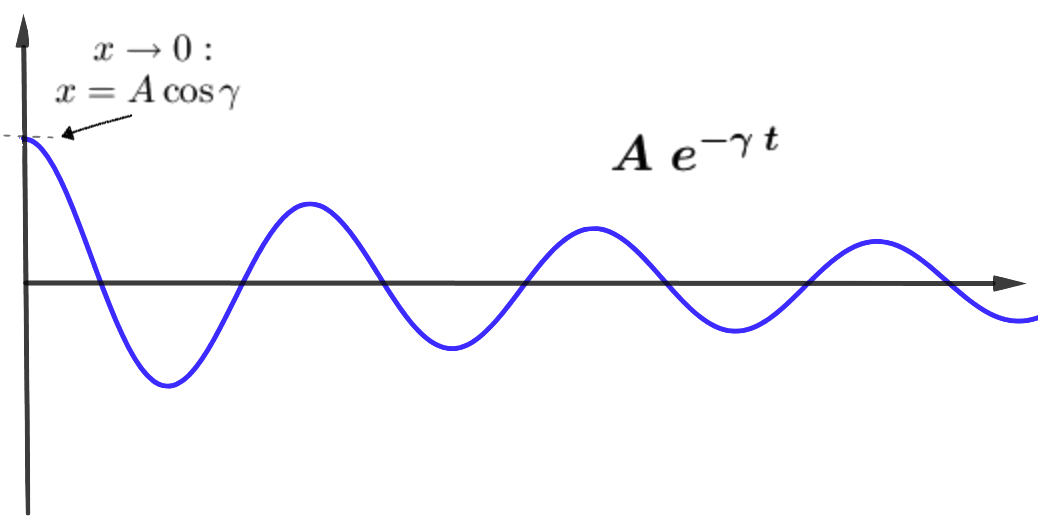
\includegraphics[width=.45\textwidth]{imagenes/img04-04.png}
	\end{figure}
\end{multicols}

\item $\gamma > \omega \qquad$ (raíces $p$ reales y distintas - \emph{sobreamortiguado})

$p_1=-\gamma + (\gamma^2-\omega^2)^{1/2}=-\gamma_1; \quad
p_2=-\gamma - (\gamma^2-\omega^2)^{1/2}=-\gamma_2 $

La solución más general es: $\theta=Ae^{-\gamma_1 t}+Be^{-\gamma_2 t}$

\begin{multicols}{2}
Exponenciales decrecientes; en este caso, la amplitud decae más rápidamente que en el anterior.

Es el caso de un péndulo muy ligero oscilando sumergido en agua.
\begin{figure}[H]
		\centering
		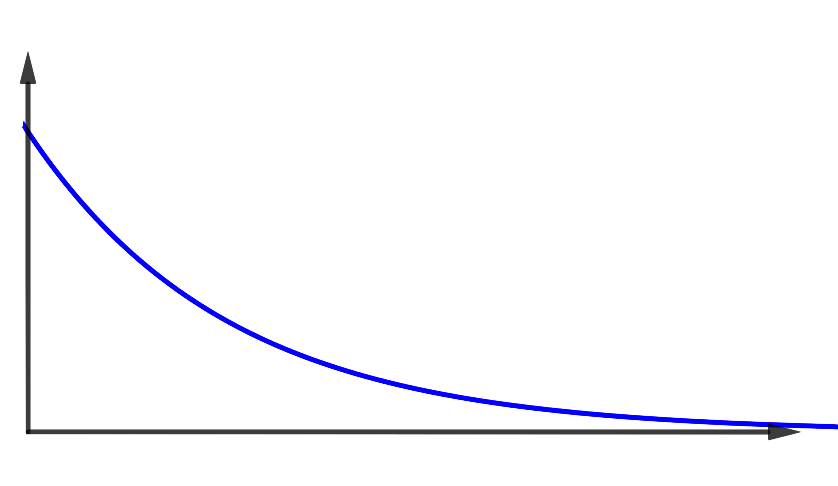
\includegraphics[width=.45\textwidth]{imagenes/img04-05.png}
	\end{figure}
\end{multicols}
\item $\gamma = \omega \qquad$	($p$ es una raíz real doble - \emph{amortiguamiento crítico})

$p=-\gamma  \to \theta=(A+Bt)e^{-\gamma t}$

\end{itemize}
\vspace{2mm}
\begin{multicols}{2}
 El amortiguamiento crítico proporciona la forma más rápida de aproximar a cero la amplitud de un oscilador amortiguado. Con menor amortiguamiento (subamortiguación) alcanza el cero más rápidamente, pero oscila alrededor de él. Con mas amortiguamiento (sobreamortiguación), el acercamiento a cero es más lento. La amortiguación crítica, ocurre cuando el coeficiente de amortiguación es igual a la frecuencia de resonancia sin amortiguación del oscilador.


\begin{figure}[H]
		\centering
		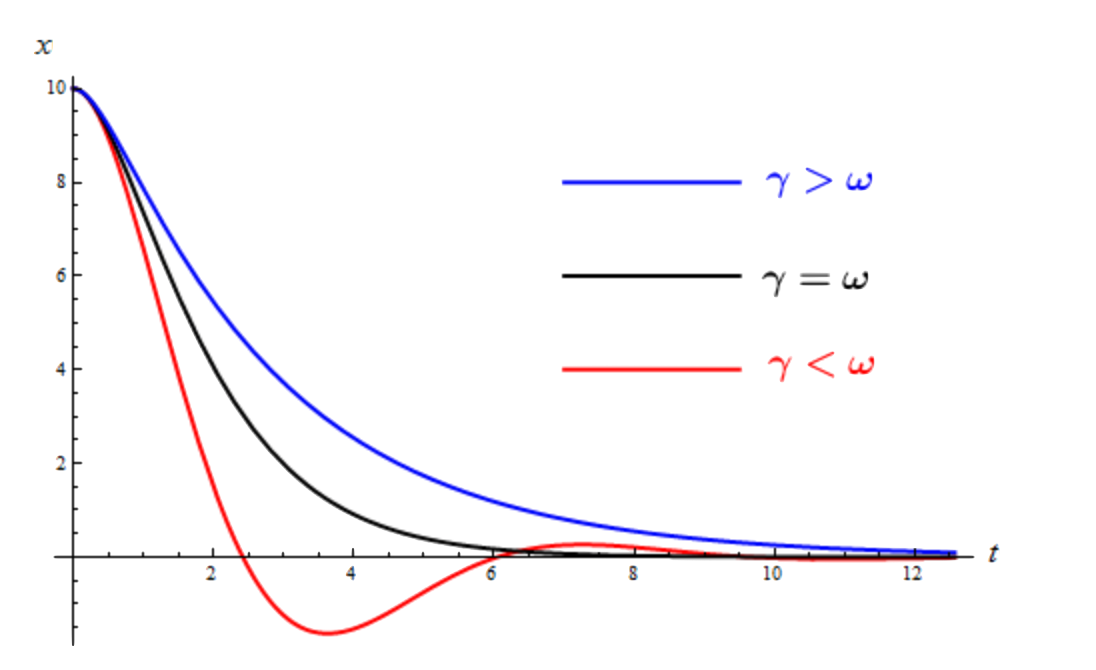
\includegraphics[width=.5\textwidth]{imagenes/img04-06.png}
	\end{figure}

\end{multicols}
\end{small}

\rule{300pt}{0.1pt}
\begin{flushright} \begin{footnotesize}
	\textcolor{gris}{`Fisica General', Ignacio Vallés, http://igvaori.github.io}
\end{footnotesize} \end{flushright}


\end{myexampleblock}


\chapter{Ejemplo \emph{Euler-Lagrange} Rotación 2D}

	\begin{tikzpicture}
	\fill [left color=red!50, right color=teal!50] (0,0) rectangle (6.5,.1);
	\fill [left color=teal!50, right color=blue!50] (6.5,0) rectangle (11.5,.1);
	\end{tikzpicture}

\vspace{1cm}
\begin{adjustwidth}{50pt}{50pt}
\begin{ejemplo}
Veremos la forma que adopta el lagrangiano para un sistema de partículas en el que no actúan fuerzas externa y que giran entorno al CM (aparece la energía cinética de traslación del CM y la de rotación en torno al CM).
\end{ejemplo}
\end{adjustwidth}

%\vspace{0.5cm}


\section{Ejemplo \emph{Euler-Lagrange} Rotación 2D}
\label{T5ELroracion}

%\vspace{5mm}

\begin{example}

\begin{multicols}{2}
Dos masas $M$ y $m$unidas por una barra rígida de masa despreciable (ligadura).

\vspace{2mm} No hay rozamiento y sobre las masas no actúa ninguna fuerza externa.
	\begin{figure}[H]
		\centering
		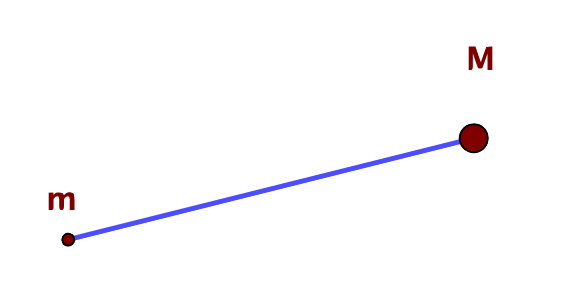
\includegraphics[width=.4\textwidth]{imagenes/img05-01.png}
	\end{figure}
\end{multicols}	
\end{example}

\vspace{3mm}
\ul{Inciso-1} $\quad$ \rule{150pt}{0.1pt} $\quad$ \textbf{Centro de masas.}

Consideremos des masas, $M$ y $m$, sobre una superficie horizontal sin fricción sobre las que no actúa ninguna fuerza neta.
\begin{multicols}{2}
	
	\begin{figure}[H]
		\centering
		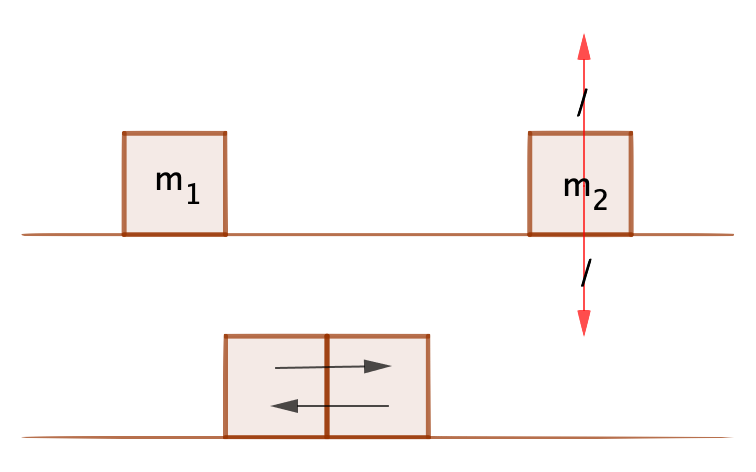
\includegraphics[width=.4\textwidth]{imagenes/img05-02.png}
	\end{figure}
	
	Durante el choque, cada cuerpo nota la fuerza que el orro ejerce sobre él y responde (3a de Newton) con una fuerza igual pero de sentido contrario.
	
$ \overrightarrow F_1=-\overrightarrow F_2 \qquad \ m_1\overrightarrow a_1=-m_2 \overrightarrow a_2	$
\end{multicols}

Integrando: $\ \displaystyle \int m_1 \vec a_1 	\dd t=-\int m_2 \vec a_2 \dd t \ \to \ m_1\vec v_1=-m_2\vec v_2+\overrightarrow A \textcolor{gris}{(\overrightarrow {cte})}$

Volviendo a integrar: $\ \displaystyle \int m_1\vec v_1 \dd t= - \int m_2\vec v_2 \dd t+ \int \overrightarrow A \dd t \ \to \ 
m\vec r_1 = -m_2\vec r_2 +\overrightarrow A t + \overrightarrow B$

Despejando, $\ m\vec r_1 + m_2\vec r_2 = \overrightarrow A t + \overrightarrow B \ \leadsto \ $ dimensiones de [M $\cdot$ L]

Dividiendo por la suma de masas: 
 $\ \dfrac{ m\vec r_1 + m_2\vec r_2}{m_1+m_2} = 
 \dfrac{ \overrightarrow A t + \overrightarrow B} {m_1+m_2} \ \leadsto \ $ dimensiones de [L]
 
 Llamamos $ \ \boldsymbol{ \overrightarrow R(t) \ = \ \dfrac{ m\vec r_1 + m_2\vec r_2}{m_1+m_2} } \quad = \dfrac{\overrightarrow B}{m_1+m_2} + \dfrac{\overrightarrow A}{m_1+m_2} t $
 
 Para $t=0 \ \to \ \overrightarrow R(0)=\dfrac{\overrightarrow B}{m_1+m_2} \ \to \overrightarrow R(t)=\overrightarrow R (0) + \dfrac{\overrightarrow A}{m_1+m_2} \ t \ \leadsto \ $ dimensiones [L], por lo que  $\dfrac{\overrightarrow A}{m_1+m_2} \ \leadsto \ $ dimensiones [LT$^{-1}$], con lo que llamamos $\ \overrightarrow V = \dfrac{\overrightarrow A}{m_1+m_2} $
 
 Finalmente: 
 
 \begin{equation}
 \overrightarrow R(t) \ = \ \overrightarrow R(0) \ + \ \overrightarrow V \ t	
 \end{equation}
 
 Dos masas sobre las que no actúa ninguna fuerza externa, solo actúan fuerzas internas (como en el momento del choque) aparece un vector $\overrightarrow R$ que viaja con MRU \textcolor{gris}{(movimiento rectilíneo y uniforme)}. $\overrightarrow R$ es la \textbf{posición del \emph{centro de masas}} y $\overrightarrow V$ es la \textbf{velocidad del \emph{centro de masas}}: $\ \overrightarrow R=\overrightarrow R_{CM};\ \ \overrightarrow V=\overrightarrow V_{CM}$
 
 Por ello, $\ \boldsymbol{ \overrightarrow V= }\displaystyle \dv{t} \overrightarrow R = \boldsymbol{ \dfrac{m_1\vec v_1 + m_2 \vec v_2}{m_1+m_2} }$
 
 Todo esto es generalizable al caso de N partículas:
 
 \begin{equation}
 \boldsymbol{
 \overrightarrow R \ =  \  \dfrac{ \displaystyle \sum_{i=1}^N m_i \ \vec r_i	}{ \displaystyle \sum_{i=1}^N m_i} \, ; \qquad  \qquad
  \overrightarrow V \ =  \  \dfrac{ \displaystyle \sum_{i=1}^N m_i \ \vec v_i	}{\displaystyle \sum_{i=1}^N m_i}
  }
 \end{equation}

\begin{flushright} \rule{300pt}{0.1pt}	\end{flushright}



	\begin{figure}[H]
	\centering
	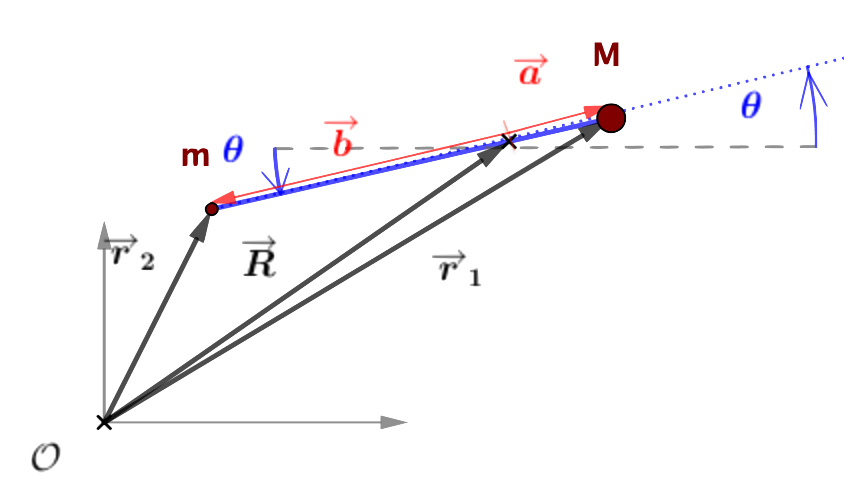
\includegraphics[width=.6\textwidth]{imagenes/img05-03.png}
	\end{figure}
	


Vamos a por el lagrangiano, en nuestro caso, $ \ L=T-\cancel{V}=T =T_1+T_2\, , \ $  \textcolor{gris}{($\  \nexists  \overrightarrow F^{ext}$ )}

$\begin{cases}
\ \vec r_1 = \overrightarrow R + \vec a  \to \vec v_1= \overrightarrow V + \dot{\vec a}
\\ \ \vec r_2=\overrightarrow R + \vec b	 \to \vec v_2=\overrightarrow V + \dot{\vec b}
\end{cases}  $

$\begin{cases} 
\ \vec a=a(\cos \theta, \sin \theta) \quad \ \ \to \ \dot{\vec a}=a\dot \theta (-\sin \theta,\cos \theta ) \ \to \ |\vec a|^2=a^2 \dot \theta^2 \\
\ \vec b=b(-\cos \theta, -\sin \theta)  \to \ \dot{\vec b}=b\dot \theta (sin \theta,-\cos \theta ) \ \, \to \ |\vec b|^2=b^2 \dot \theta^2 
\end{cases}$ \begin{footnotesize} $\ \  \textcolor{gris}{(\sin^2 \theta + …\cos^2 \theta=1)}$ \end{footnotesize}

$\begin{cases}
\ v_1^2=V^2+|\vec a|^2+2\vec v \cdot \dot{\vec a} \\	
\ v_2^2=V^2+|\vec b|^2+2\vec v \cdot \dot{\vec b}
\end{cases} \quad \to \qquad T=\dfrac M 2 \ v_1^2 + \dfrac m 2 \ v_2^2$ 

$T=\dfrac 1 2 {(M+m)} V^2 + \dfrac M 2 |\dot{\vec a}|^2 + \dfrac m 2 |\dot{ \vec b}|^2 + M \overrightarrow V \cdot \dot{\vec a}+ m \overrightarrow V \cdot \dot{\vec b} $

$T=\dfrac 1 2 {(M+m)} V^2 + \dfrac M 2 |\dot{\vec a}|^2 + \dfrac m 2 |\dot {\vec b}|^2 +\overrightarrow V \cdot (M\dot{\vec a} + m\dot{\vec b})$

$T=\dfrac 1 2 {(M+m)} V^2 + \dfrac M 2 |\dot{\vec a}|^2 + \dfrac m 2 |\dot {\vec b}|^2 +
\overrightarrow V \cdot \cancelto{0}{ \displaystyle \dv{t} (M \vec a + m \vec b)}$

\vspace{7mm} 
\ul{Inciso-2} $\quad$ \rule{150pt}{0.1pt} $\quad$ 

$V \cdot  \displaystyle \dv{t} (M \vec a + m \vec b) = 
V \cdot  \displaystyle \dv{t} [M (\vec r_1-\overrightarrow R) + m (\vec r_2-\overrightarrow R)]=
V \cdot  \displaystyle \dv{t} [M\vec r_1+m\vec r_2 - (M+m) \overrightarrow R ]=
V \cdot  \displaystyle \dv{t} [M\vec r_1+m\vec r_2 - \cancel{(M+m)} \dfrac{M\vec r_1 + m \vec r_2}{ \cancel{M+m}}]=
V \cdot \displaystyle \dv{t} \ 0 =0$

\begin{flushright} \rule{300pt}{0.1pt}	\end{flushright}

\vspace{5mm}

Luego, $ \ T=\dfrac 1 2 {(M+m)} V^2 + \dfrac M 2 |\dot{\vec a}|^2 + \dfrac m 2 |\dot {\vec b}|^2$

Sustituyendo los valores obtenidos para $|\dot{\vec a}|^2 \text{ y } |\dot{\vec b}|^2 $,

$L=T=\dfrac 1 2 {(M+m)} V^2 + \left[ \dfrac M 2 a^2 + \dfrac m 2 b^2 \right] \ \dot \theta^2 =
\dfrac 1 2 {(M+m)} V^2 + \dfrac 1 2 \left[  M  a^2 +  m  b^2 \right] \ \dot \theta^2$

\begin{equation}
\subrayado{ \boxed{ \ \boldsymbol{
 L \ = \ \dfrac 1 2 \ {(M+m)} \ V^2 \ + \ \dfrac 12 \ I_{CM} \ \omega^2
  } \  } }
 \end{equation}
 
 donde $\ I_{CM}\ $ es el \emph{momento de inercia} respecto el centro de masas.

\vspace{5mm}	
\ul{Inciso-3} $\quad$ \rule{150pt}{0.1pt} $\quad$ \textbf{Momento de inercia}

\begin{multicols}{2}
En MCU \begin{footnotesize}  (movimiento circular uniforme) \end{footnotesize}

$\overrightarrow L=\vec r \times \vec p = \vec r \times m \vec v$

$|\overrightarrow L |=rmv \sin \dfrac \pi 2 =m\ r \ v$

$v=\omega r \to L=mr\omega r=(mr^2)\  \omega$
\begin{figure}[H]
	\centering
	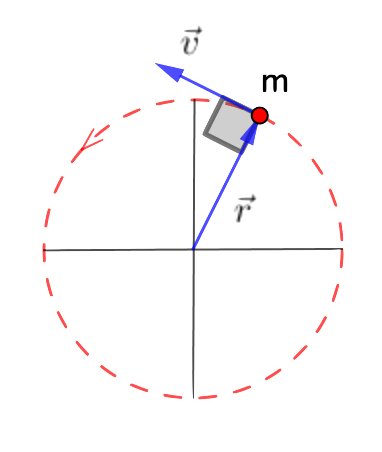
\includegraphics[width=.25\textwidth]{imagenes/img05-06.png}
	\end{figure}	
\end{multicols}

El factor $mr^2\ $ depende de la geometría del sistema y se llama \textbf{\emph{Momento de Inercia}}

	

\vspace{5mm}
Para N partículas ligadas girando en torno al CM con la misma $\omega$,

$$\boldsymbol{}I\ = \ \dfrac{\displaystyle \sum_{i=1}^N m_i \ r_i^2}{\displaystyle \sum_{i=1}^N m_i}\, ; \qquad L \ = \ I \ \omega$$
\begin{flushright} \rule{300pt}{0.1pt}	\end{flushright}

\vspace{5mm}

\begin{myalertblock}{Lagrangiano con rotación}
\begin{large}
\begin{equation}
\label{T5Lconrotacion}
\boldsymbol{
L \ = \ \dfrac{M_{TOTAL}}{2}\ \ V_{CM}^2 \ + \ \dfrac 1 2 \ I_{CM}\  \ \dot \theta^2
} 
\end{equation}	
\end{large}
\end{myalertblock}

Forma que adopta el lagrangiano para un sistema de partículas en el que no actúan fuerzas externa y que giran entorno al CM (aparece la energía cinética de traslación del CM y la de rotación en torno al CM).

	

	
	
	
	
	








\chapter{Ejemplo \emph{Euler-Lagrange}. Modos Normales}

	\begin{tikzpicture}
	\fill [left color=red!50, right color=teal!50] (0,0) rectangle (6.5,.1);
	\fill [left color=teal!50, right color=blue!50] (6.5,0) rectangle (11.5,.1);
	\end{tikzpicture}

\vspace{10mm}
\begin{adjustwidth}{50pt}{50pt}
\begin{ejemplo}
	Veremos como aparecen los modos normales de oscilación al desacoplar el lagrangiano diagonalizando el problema.
\end{ejemplo}
\end{adjustwidth}


\section{Ejemplo \emph{Euler-Lagrange} Modos Normales}

\vspace{5mm}
\begin{example}
.	Tres partículas de masas $m$	 unidas por dos muelles de constantes elásticas $k$, situadas en una superficie horizontal sin rozamiento (no tenemos en cuenta la fuerza de la gravedad, para mayor claridad didáctica).

	\begin{figure}[H]
		\centering
		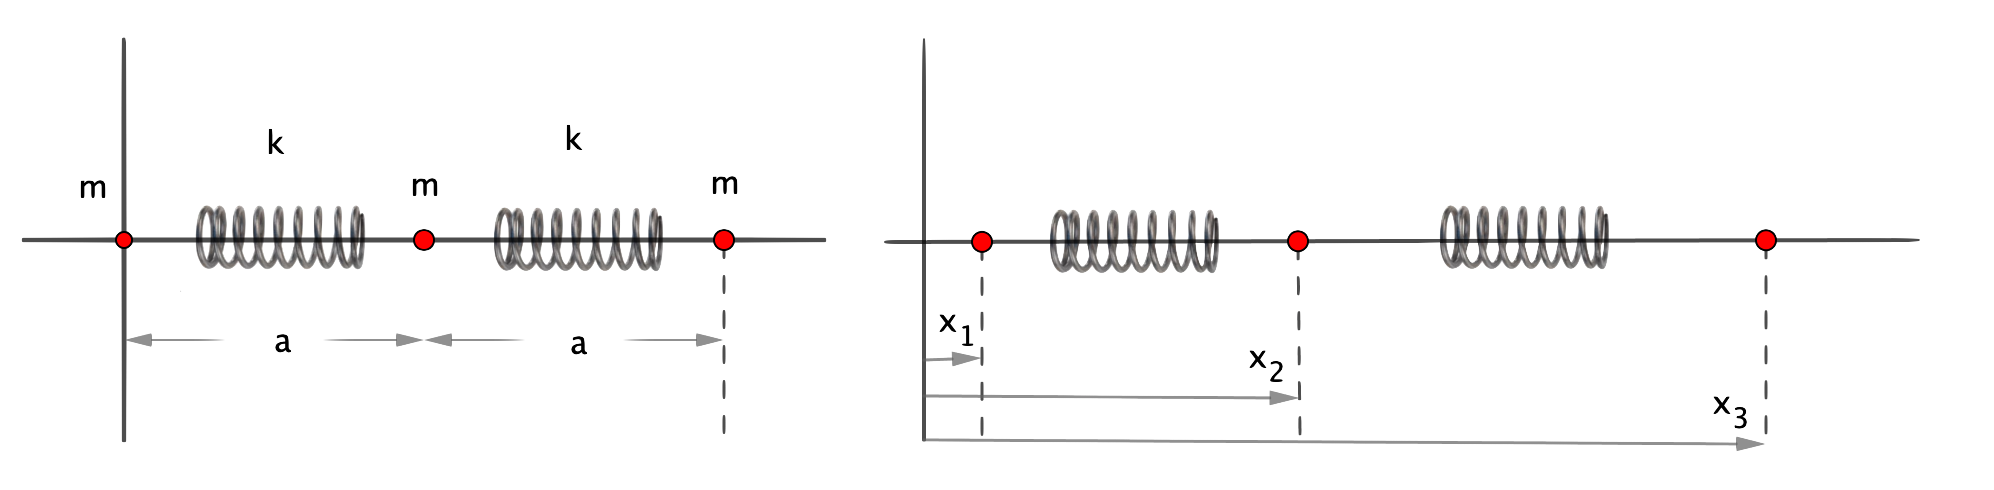
\includegraphics[width=1\textwidth]{imagenes/img06-01.png}
	\end{figure}
\end{example}
\vspace{5mm}

Si$a$ es la longitud natural del muelle, cuando se estira hasta que su longitud aumenta a $L$, la energía potencial es $V=\dfrac k 2 (L-a)^2$, en nuestro caso: 

$V_{muelle 1}=\dfrac k 2 (2_2-x_1-a)^2\, ; \quad 
V_{muelle 2}=\dfrac k 2 (x_3-x_2-a)^2 \quad \to $ 

\hspace{2cm} $\to \quad V\ = \ \dfrac k 2 \  \left[ \ (2_2-x_1-a)^2 \ + \ (x_3-x_2-a)^2  \  \right]$

Vamos a establecer un \emph{cambio de variable} para evitar esta molesta $\ a$:

\begin{equation}
\label{T6VC1}
\begin{cases}
\ \ x_1  \ = \  y_1	\\
\ \ x_2  \ = \ a\ + \ y_2 \\
\ \ x_3 \ = \ 2a\ + \ y_3
\end{cases} \quad \to \quad \qquad \textcolor{gris}{
\begin{cases}
\ \ \dot x_1  \ = \   \dot y_1	\\
\ \ \dot x_2  \ = \   \dot y_2 \\
\ \ \dot x_3  \ = \   \dot y_3
\end{cases} }
\end{equation}


$V=\dfrac k 2 \ \left[ \ 
(a+y_2-(y_1)-a)^2 \ + \ (2a+y3-(a+y_2)-a)^2)
\ \right] =
\dfrac k 2 [\ (y_2-y_1)^2 \ + \ (y_3-y_2)^2 \ ]$

Vamos con la energía cinética:

$T=\dfrac 1 2 m \ \dot x_1^2 + \dfrac 1 2 m \ \dot x_2^2 + \dfrac 1 2 m \ \dot x_3^2 \ = \ \dfrac m 2 \ [\ \dot x_1^2  + \dot x_2^2 + \dot x_3^2\ ]  = \ \dfrac m 2 \ [\ \dot y_1^2  + \dot y_2^2 + \dot y_3^2\ ]  $

Luego, 

\begin{equation}
\subrayado{
\boldsymbol{
L \ = \ 
\dfrac m 2 \ [\ \dot y_1^2  + \dot y_2^2 + \dot y_3^2\ ]
\ - \ 	
\dfrac k 2 [\ (y_2-y_1)^2 \ + \ (y_3-y_2)^2 \ ] 
} }
\end{equation}

Si a este lagrangiano le aplicamos las ecuaciones de Euler-Laplace (ec. \ref{T2EEL1C}), obtendríamos unas EDOs lineales, homogéneas pero \emph{acopladas}. Para solucionarlo vamos a hacer un \emph{truco: DIAGONALIZACION}\footnote{Recordamos la diagonalización de una matriz al final del tema (Nota - 1) } 

Desarrollamos la parte del potencial:

$(y_2-y_1)^2  +  (y_3-y_2)^2 = y_2^2+y_1^2-2y_1y_2 + y_3^2+y_2^2-2y_2y_3 =
\textcolor{red}{\underline{1}} \ y_1^2 + \textcolor{red}{\underline{2}} \ y_2^2 +\textcolor{red}{\underline{1}} \ y_3^2-\textcolor{blue}{\underline{2}} \ y_1y_2-\textcolor{teal}{\underline{2}} \ y_2y_3 \overrightarrow{=} $

Matricialmente, $\quad \overrightarrow{= } \ 
\mqty(y_1&y_2&y_3)\ \mqty ( \textcolor{red}{1}&\textcolor{blue}{-1}&0\\\textcolor{blue}{-1}&\textcolor{red}{2}&\textcolor{teal}{-1}\\0&\textcolor{teal}{-1}&\textcolor{red}{1})\ \mqty(y_1\\y_2\\y_3)$  

Al diagonalizar esta matriz, obtenemos como valores propios y vectores propios \emph{normalizados}:


$$\vec c_1=\dfrac 1 {\sqrt{3}} \mqty(1\\1\\1) \,; \ \ \lambda_1=0\,; \qquad
\vec c_2=\dfrac 1 {\sqrt{2}} \mqty(-1\\0\\1) \,; \ \ \lambda_2=1\,; \qquad
\vec c_3=\dfrac 1 {\sqrt{6}} \mqty(1\\-2\\1) \,; \ \ \lambda_3=3$$

La matriz de cambio de base es:

\begin{equation}
\label{T6matrizcambiobase.ortogonal}	
M\ = \ \mqty(1/\sqrt{3} & -1/\sqrt{2} & 1/\sqrt{6} \\ 1/\sqrt{3} & 0 & -2/\sqrt{6} \\ 1/\sqrt{3} & 1/\sqrt{2} & 1/\sqrt{6})
\end{equation} 

Con la cual establecemos un segundo cambio de variable:

\begin{equation}
\label{T6VC2}
\mqty(y_1\\y_2\\y_3) \ = \ M\ \mqty(z_1\\z_2\\z_3) \quad \to \qquad
\begin{cases}
\ \ y_1=z_1/\sqrt{3} - z_2/\sqrt{2}+z_3/\sqrt{6}\\
\ \ y_2=z_1\sqrt{3}\quad \quad - \quad \quad 2z_2/\sqrt{6}\\
\ \ y_3=z_1/\sqrt{3}+z_2/\sqrt{2}+z_3/\sqrt{6}	
\end{cases}	
\end{equation}


Sustituyendo estos valores en la expresión anterior que provenía de la parte potencial, tenemos:

$\begin{small} (y_2-y_1)^2  +  (y_3-y_2)^2 =
\textcolor{red}{\underline{1}} \ y_1^2 + \textcolor{red}{\underline{2}} \ y_2^2 +\textcolor{red}{\underline{1}} \ y_3^2-\textcolor{blue}{\underline{2}} \ y_1y_2-\textcolor{teal}{\underline{2}} \ y_2y_3 \end{small} =
\ \boldsymbol{0}\ z_1^2 \ + \ \boldsymbol{1} \ z_2^2 \ + \ \boldsymbol{3} \ z_3^2$

\textcolor{gris}{($\boldsymbol{0,1,3}$ son los valores propios de la matriz.)}

Esto facilita mucho la obtención de las ecuaciones de movimiento al aplicar Euler-Lagrange, pues se obtienen EDOs \emph{desacopladas}. Esto es \emph{diagonalizar} el problema o obtener los \emph{modos normales} (lo que en teoría cuántica de campos se convertirán en partículas).

En cuanto a la parte cinética del lagrangiano, este cambio de base (diagonalización queda \emph{invariable}).\footnote{Justificación al final del capítulo. (Nota - 2)}

\begin{equation}
\label{T6inavraible}
\dot y_1^2 \ + \dot y_2^2 \ + \dot y_3^2 \ = \dot z_1^2 \ + \dot z_2^2 \ + \dot z_3^2  
\end{equation}

Con esta diagonalización, el lagrangiano adopta la siguiente forma:


\begin{equation}
\subrayado{
	\boldsymbol{
		L\ =\ \dfrac 1 2 \ m \ [ \ \dot z_1^2 \ + \dot z_2^2 \ + \dot z_3^2 \ ]\ + \ \dfrac k 2 \ [\ z_2^2  + \ z_3^2 \ ]
	}	}
\end{equation}

Y, ahora sí, vamos a aplicar las ecuaciones de Euler-Lagrange:






\begin{myblock}{Ecuaciones Euler-Lagrange}
\begin{equation}
\boxed{ \ 
\dv{t} \left( \pdv{L}{\dot q_i} \right) \ - \ \pdv{L}{q_i} \ = \ 0	
\ }
\textcolor{gris}{\qquad \qquad q_i=z_1,\ z_2,\ z_3 \text{ en este caso}}
\tag{\ref{EELconservativas}}
\end{equation}
\end{myblock}

$\boxed{ \ \boldsymbol{z_1} \ } \quad \Rightarrow \ \ \ $
$\displaystyle \dv{t} \left( \pdv{L}{\dot z_1} \right) \ - \ \cancelto{0}{\pdv{L}{z_1}} \ = \ 0 \quad \to \quad \dv{t} \left( \pdv{L}{\dot {z_1}} \right)=0 \quad \to \qquad \pdv{L}{\dot{z_1}}= \ \ \boxed{\ \boldsymbol{ m\dot{z_1}\ = \ cte } \ }$ 

$\boxed{ \ \boldsymbol{z_2} \ } \quad \Rightarrow \ \ \ $
$\displaystyle \dv{t} \left( \pdv{L}{\dot z_2} \right) \ - \ \cancelto{0}{\pdv{L}{z_2}} \ = \ 0 \quad \to \quad \dv{t}(m\dot{z_2})+\dfrac k 2 z_2=0 \quad \to \qquad  \boxed
{ \bold{\ m\ddot{z}_2 \ -k_2\ z_2\ = 0\ }}$

$\boxed{ \ \boldsymbol{z_2} \ } \quad \Rightarrow \ \ \ $
Análogamente, $\qquad  \boxed{ \bold{\ m\ddot{z}_3 \ -k_2\ z_3\ = 0\ }}$


\vspace{0.5cm}
Las ecuaciones diferenciales desacopladas de movimiento son:
\begin{equation}
\begin{cases}
\ \ \ \boldsymbol{ m\ \dot{z_1}\ = \ cte }
\\
\ \ \bold{\ m\ \ddot{z}_2 \ -k_2\ z_2\ = 0\ }
\\
\ \ \bold{\ m\ \ddot{z}_3 \ -k_2\ z_3\ = 0\ }	
\end{cases}
\end{equation}
%\vspace{0.5cm}

$E-L \ : \ \  z_1 \quad \Rightarrow \quad \boldsymbol{  z_1 \ = A t \ + \ B }$

$E-L \ : \ \ z_2 \quad \Rightarrow \quad $ EDO segundo orden lineal homogénea:

\begin{adjustwidth}{10mm}{5mm}
$m f''(t)=-kf(t) \to f''(f)=-\dfrac k m f(t) \to \lambda^2-\dfrac k m =0 \to RRS:\ \lambda=\pm \sqrt{\dfrac k m}$

$f(t)=a\ e^{i\lambda_1 t}\ + \ b \ e^{i\lambda_2 t}\ $
Llamando $\ \omega_0=\sqrt{\dfrac k m }\, ,\  $ frecuencia de oscilación del muelle,

$f(t)=a(cos \omega_0 t+i\sin \omega_0 t)+b(\cos \omega_0 t-i\sin \omega_0 t)= c_1 \cos \omega_0 t + i c_2 \sin \omega_0 t\, , \ $ 

con $ \ c_1=(a+b) \text{ y } c_2=(a-b) \in \mathbb R $

Por trigonometría, todo seno se puede escribir como un coseno (y viceversa), por lo que 

$\ f(t)=D \cos (\omega_0 t + F)\, \ $ con lo que $ \qquad \boldsymbol{z_2 \ = \ C\ (\cos \omega_0 t \ + \  D)}$
\end{adjustwidth}




$E-L \ : \ \ z_3 \quad \Rightarrow \quad $ Como $\ddot {z_3}=-3\dfrac k m z_3=(\sqrt{3} \omega_0)^2 \ z_3 \quad \to \quad \boldsymbol{z_3 \ = \ F\ \ (\cos \sqrt{3} \omega_0 t \ + \ G)}$

\vspace{5mm}
Hemos obtenido como soluciones a las ecuaciones diferenciales de movimiento:

\begin{equation}
\begin{cases}
\ \ \boldsymbol{  z_1 \ = A t \ + \ B } \\ 
\ \ \boldsymbol{z_2 \ = \ C\ (\cos \omega_0 t \ + \  D)} \\
\ \ \boldsymbol{z_3 \ = \ F\ \ (\cos \sqrt{3} \omega_0 t \ + \ G)}	
\end{cases}
\end{equation}


\vspace{5mm}
Solo falta deshacer los dos cambios de variable que hemos realizado, ecuaciones \ref{T6VC2} y \ref{T6VC1}:

$\begin{cases}
\ \ y_1=\dfrac B {\sqrt{3}} \ + \ \dfrac A{\sqrt{3}} - \dfrac C {\sqrt{2}} \ \cos (\omega_0t+D) + \dfrac F{\sqrt{6}} \ \cos(\sqrt{3} \omega_0 t + G)	 \\
\ \ y_2=\dfrac B {\sqrt{3}} \ + \ \dfrac A{\sqrt{3}}  
\qquad \qquad \qquad \qquad \ \ - \sqrt{\dfrac 2 3 } \ F  \ \cos(\sqrt{3} \omega_0 t + G)	  \\
\ \ y_3=\dfrac B {\sqrt{3}} \ + \ \dfrac A{\sqrt{3}} + \dfrac C {\sqrt{2}} \ \cos (\omega_0t+D) + \dfrac F{\sqrt{6}} \ \cos(\sqrt{3} \omega_0 t + G)	
\end{cases}$

\vspace{5mm}
Finalmente,

$\begin{cases}
\ \ x_1=\dfrac B {\sqrt{3}} \ + \ \dfrac A{\sqrt{3}} - \dfrac C {\sqrt{2}} \ \cos (\omega_0t+D) + \dfrac F{\sqrt{6}} \ \cos(\sqrt{3} \omega_0 t + G)	 \\
\ \ x_2=\dfrac B {\sqrt{3}} \ + \ \dfrac A{\sqrt{3}}  
\qquad \qquad \qquad \qquad \ \ - \sqrt{\dfrac 2 3 } \ F  \ \cos(\sqrt{3} \omega_0 t + G)	\boldsymbol{ \ + \ a}  \\
\ \ x_3=\dfrac B {\sqrt{3}} \ + \ \dfrac A{\sqrt{3}} + \dfrac C {\sqrt{2}} \ \cos (\omega_0t+D) + \dfrac F{\sqrt{6}} \ \cos(\sqrt{3} \omega_0 t + G)	\boldsymbol{\ \  \ + \ 2a}
\end{cases}$

\vspace{5mm}
Ecuaciones de movimiento que podemos escribir \emph{vectorialmente} como:

\begin{equation}
\label{T6sol}
\subrayado{
\mqty(x_1\\x_2\\x_3)=
\mqty(0\\a\\2a) +
(B+At)\ \mqty(\dfrac 1{\sqrt{3}}\\ \dfrac 1{\sqrt{3}} \\ \dfrac 1{\sqrt{3}} )+
C\ \cos(\omega_0t+D)\ \mqty(- \dfrac 1 {\sqrt{2}} \\0\\ \dfrac 1 {\sqrt{2}})+
F\ \cos(\sqrt{3}\omega_0t+G)\ \mqty(\dfrac 1{\sqrt{6}}\\-\sqrt{\dfrac 2 3 }\\ \dfrac 1{\sqrt{2}})	
}
\end{equation}

Han aparecido los vectores propios $\vec c_1, \ \vec c_2, \ \vec c_3$ y los valores propios $\sqrt{\lambda_1},\ \sqrt{\lambda_2},\ \sqrt{\lambda_3}$con los $\omega_0$ de la diagonalización del problema.

Las soluciones numéricas de estas ecuaciones muestran:

Ponemos D=G=0, no hay desfase inicial.

Haciendo F=0, C=1, A=0, obtenemos la figura 1, las partículas de los extremos oscilan en sentidos contrarios y la del centro está fija.

Desactivamos un nodo y activamos el otro: C=0, F=1. Obtenemos la figura 2, el sistema total oscila y la partícula central los hace del mismo modo.

Activando los dos modos C=F=1, obtenemos un movimiento más complicado.

\vspace{5mm}
\begin{figure}[H]
		\centering
		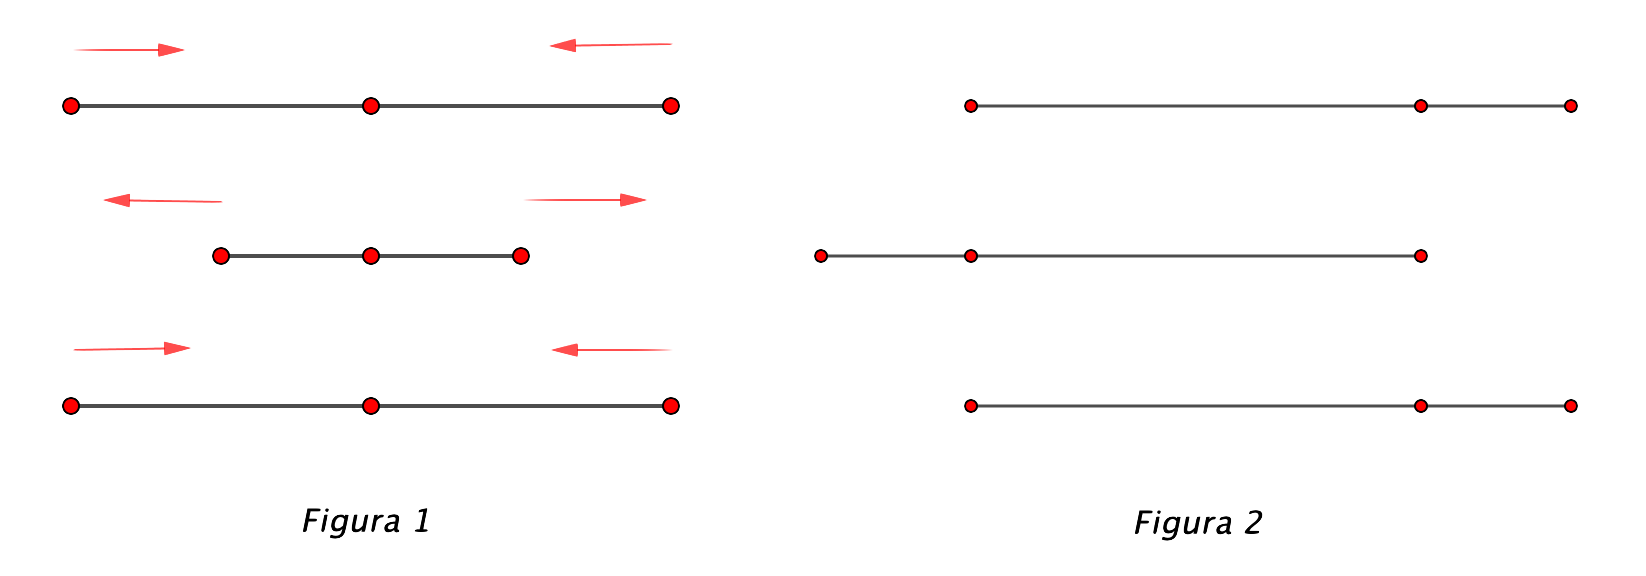
\includegraphics[width=1\textwidth]{imagenes/img06-02.png}
	\end{figure}

Los cuatro términos de las soluciones obtenidas, ec \ref{T6sol}, son:

\begin{adjustwidth}{20pt}{20pt}
\begin{itemize}
\item Vector desplazamiento, que tiene en cuenta la colocación de las masas.
\vspace{-3mm} \item MRU del CM.
\vspace{-3mm} \item un modo normal de oscilación.
\vspace{-3mm} \item otro modo normal de oscilación.	
\end{itemize}
\end{adjustwidth}

Las partes responsables del lagrangiano son, la \textcolor{red}{energía cinética} responde del MRU del CM y la \textcolor{blue}{energía potencial} de los osciladores armónicos.

	$$\boldsymbol{
		L\ =\ \textcolor{red}{\dfrac 1 2 \ m \ [ \ \dot z_1^2 \ + \dot z_2^2 \ + \dot z_3^2 \ ]} \ + \ \textcolor{blue}{\dfrac k 2 \ [\ z_2^2  + \ z_3^2 \ ]}
	}$$	


\vspace{1cm}

\begin{ejemplo}
	\subsection{Nota 1: Diagonalización de una matriz}
\end{ejemplo}
	
	\begin{myexampleblock}{Diagomalización de una matriz}
		
		\vspace{2mm} \emph{Diagonalizar}\footnote{$\ $ --- Capítulo 8 'Diagonalización de matrices`,  \emph{``Álgebra lineal y geometría (avanzadas) para bachillerato''}, \textcolor{blue}{Ignacio Vallés, http://igvaori.github.io} $\quad$  --- Apéndice \ref{ApendiceDiagonalizacion} `Diagonalización de matrices'} una matriz cuadrada $A$, $n\times x$ ,cosiste en encontrar unos número reales $\lambda_i$ llamados \emph{valores propios} y unos vectores $\vec c_i$, $n\times 1$, llamados \emph{vectores propios}, tales que se cumpla:
		
		$$\boldsymbol{ A \ \vec c \ = \ \lambda \ \vec c }$$
		
	Para ello, encontraremos las soluciones de la ecuación $\ |A-\lambda I|=0$, los valores propio $\lambda_i$. Para cada un de ellos buscaremos los vectores que cumplan $\ (A-\lambda_i I)\  \vec c_i \ = \ 0$, los vectores propios.
		
	\vspace{2mm} \textcolor{gris} {$A\vec c=\lambda \vec c \to A\vec c - \lambda I \vec c=0 \to (A-\lambda I)\vec c=0\, ,\ $ conduce a un sistema de ecuaciones lineales \emph{homogéneo} que para que tenga solución distinta de la trivial es necesario que $|A-\lambda I|=0$. }
		
	\vspace{2mm} Encontrados los vectores propios podemos construir la matriz $M$ formada por los vectores columna $\vec c_i$ y se cumple:
		
		$$A \ = \ M \ D \ M^{-1} \ \to \ D \ = \ M^{-1} \ A \ M \ = \ diag(\lambda_i)=\mqty(\lambda_1 & 0 & \cdots &0\\
		0&\lambda2&\cdots &0\\ \vdots&\vdots&\ddots&\vdots\\0&0&\cdots&\lambda_n)$$
		
	\vspace{2mm}\textcolor{gris}{La elección e los vectores $\vec c_i$ se hará exigiendo que estén \emph{normalizados}, $\boldsymbol{|\vec c_i|=1}$, y de modo que $\boldsymbol{|M|>0}$.}
	
	\vspace{3mm}Teoremas:
	\begin{itemize}
	\item $A=A^T \text{ (simétrica) } \to A diagonalizable$
	\item $\vec c_i \cdot \vec c_j = c_i^T c_j = 0\in \mathbb R$, los nuevos vectores 	son \emph{ortogonales}. La matiz $M$ es \emph{ortogonal} (asociada a una \emph{rotación}).
	\item $ M \text{ ortogonal } \to M^T=M^{-1}$
	\item Por ello, $\ MM^T=M^TM=I$
	\item $A \text{ simetrica } \ \longrightarrow \ A \text{ ortogonalmente diagonalizable}$
	\end{itemize}
	
	
\begin{center}\rule{200pt}{0.1pt}\end{center}
		
\vspace{7mm}  \textbf{Diagonalizar la matriz} $ \boldsymbol{ A=\mqty(1&-1&0\\-1&2&-1\\0&-1&1)}$ 
		
\vspace{2mm}  $ |A-\lambda I|=0 \to \left| \mqty(1-\lambda&-1&0\\-1&2-\lambda&-1\\0&-1&1-\lambda) \right| = -\lambda^3+4\lambda^2-3\lambda=0 \to \begin{cases}
 \ \lambda_1=0 \\ \ \lambda_2=1 \\ \ \lambda_3=3	
 \end{cases}$		
		
\vspace{2mm} $\boldsymbol{\lambda_1=0 \to } \quad (A)\vec c_1=\vec 0 \to \mqty(1&-1&0\\-1&2&-1\\0&-1&1)\mqty(x\\y\\z)=\mqty(0\\0\\0) \to \begin{cases}
 	x-y&=0\\-x+2y-z&=0\\z-y&=0
 \end{cases}$
 
\vspace{2mm}Sistema de ecuaciones lineales compatible indeterminado, solución: $\ x=y=z=1$. 
 
\vspace{2mm}Tomando $z=1$ y racionalizando:  $\ \boldsymbol {\vec c_1=\dfrac 1 {\sqrt{3}} (1,1,1)^T}$

\vspace{2mm} $\boldsymbol{\lambda_2=1 \to } \quad \quad (A-I)\vec c_2=\vec 0 \to \mqty(0&-1&0\\-1&1&-1\\0&-1&-1)\mqty(x\\y\\z)=\mqty(0\\0\\0) \to \begin{cases}
 	-y&=0\\-x+y-z&=0\\-y&=0
 \end{cases}$
 
\vspace{2mm}Sistema de ecuaciones lineales compatible indeterminado, solución: $\ y=0;\ x=-z$. 
 
\vspace{2mm}Tomando $z=-1$ y racionalizando:  $\ \boldsymbol {\vec c_2=\dfrac 1 {\sqrt{2}} (1,0,-1)^T}$

\vspace{2mm} $\boldsymbol{\lambda_3=3 \to } \quad \quad (A-3I)\vec c_3=\vec 0 \to \mqty(-2&-1&0\\-1&-1&-1\\0&-1&-2)\mqty(x\\y\\z)=\mqty(0\\0\\0) \to \begin{cases}
 	-2x-y&=0\\-x-y-z&=0\\-y-2z&=0
 \end{cases}$
 
\vspace{2mm}Sistema de ecuaciones lineales compatible indeterminado, solución: $\ x=z=; \ y=-2z$. 
 
\vspace{2mm}Tomando $z=1$ y racionalizando:  $\ \boldsymbol {\vec c_3=\dfrac 1 {\sqrt{6}} (1,-2,1)^T}$

\vspace{2mm}Con ello, la matriz de cambio de base es $\boldsymbol{ M=\ \mqty(1/\sqrt{3} & -1/\sqrt{2} & 1/\sqrt{6} \\ 1/\sqrt{3} & 0 & -2/\sqrt{6} \\ 1/\sqrt{3} & 1/\sqrt{2} & 1/\sqrt{6})\ }$ y la matriz diagonalizada $\boldsymbol{ D=\mqty(0&0&0\\0&1&0\\0&0&3) }$


\vspace{4mm}Si en la base $A$ las coordenadas $y_1,y_2,y_3$ tienen la relación con variables \underline{acopladas}:

\vspace{2mm}$(\vec y)^T \ A \ \vec y = \mqty(y_1&y_2&y_3)\ \mqty(1&-1&0\\-1&2&-1\\0&-1&1) \ \mqty(y_1\\y_2\\y_3)=y_1^2+2y_2^2+y_3^2-2y_1y_2-2y_2y_3$, relación con variables \underline{acopladas}.

\vspace{2mm}Al diagonalizar y cambiar de base $y_i \ \to z_i$, $\mqty(y_1\\y_2\\y_3)=M \mqty(z_1\\z_1\\z_3)$ y sustituir en la relación acoplada, las nuevas coordenadas aparecen \underline{desacopladas}: $0z_1^2+1z_2^2+3z_3^2$, como vemos en

\vspace{2mm} $(\vec z)^T \ D \ \vec z= 
 \mqty(z_1&z_2&z_3)\ \mqty(0&0&0\\0&1&0\\0&0&3) \ \mqty(z_1\\z_2\\z_3)=0\ z_1^2 + 1\ z_2^2 + 3\ z_3^2$
 
\vspace{2mm} \begin{center} \rule{200pt}{0.1pt} \end{center}

Forma acoplada: $\boldsymbol{(\vec y)^T A \vec y}$; 

Cambio de variable: $\vec y=M \vec z  \ \to \ (\vec y)^T=(M \vec z)^T=(\vec z)^T M^T=(\vec z)^T M^{-1}$, 

por ello,  $(\vec y)^T A \vec y = ((\vec z)^T  M^{-1} ) \ A  \ (M  \vec z ) = (\vec z)^T \ (M^{-1} \ A \ M ) \ \vec z= \boldsymbol{(\vec z)^T D \vec z}$, forma no acoplada.

$\,$

\end{myexampleblock}

\vspace{10mm}

\begin{ejemplo}
\subsection{Nota 2: Uso de la Geometría Diferencial (tensores, métrica,...)}
Vamos a ver que el cambio de base efectuado, de $\ y_i \ \to \ z_i\, ,\  $ como la matriz del cambio es \emph{ortogonal}, deja invariante la \emph{métrica} (ecuación \ref{T6inavraible}).
$\ \ y_i \ \to \ z_i \ : \qquad  \dot y_1^2 \ + \dot y_2^2 \ + \dot y_3^2 \ = \dot z_1^2 \ + \dot z_2^2 \ + \dot z_3^2 $

Como la matriz cambio de base, ec. \ref{T6matrizcambiobase.ortogonal}
$\ M\ = \ \mqty(1/\sqrt{3} & -1/\sqrt{2} & 1/\sqrt{6} \\ 1/\sqrt{3} & 0 & -2/\sqrt{6} \\ 1/\sqrt{3} & 1/\sqrt{2} & 1/\sqrt{6})\ $ es ortogonal y de $\ |M|=1\, , \ $ se trata de una \emph{rotación} y veremos que conserva la métrica. Si antes del cambio la métrica era la \emph{identidad}, tras la rotación seguirá siéndolo.

Coordenadas de $y^\alpha:\quad \overrightarrow A\cdot \overrightarrow A = A_\alpha A^\alpha =g_{\alpha \beta}A^\alpha A^\beta = 	\delta_{\alpha \beta} A^\alpha A^\beta =(A^1)^2+(A^2)^2+(A^3)^2$

\textcolor{gris}{$	\delta_{\alpha \beta}$ es el delta de Kronecker, la identidad.}

Coordenadas de $z_\alpha:\quad \overrightarrow A\cdot \overrightarrow A = g_{{\alpha'} {\beta'}} A^{\alpha'} A^{\beta'}=  \delta_{{\alpha'} {\beta'}} A^{\alpha'} A^{\beta'} =(A^{1'})^2+(A^{2'})^2+(A^{3'})^2$

En nuestro caso no tenemos un vector $\overrightarrow A$ sino su derivada, $\ \displaystyle \dv{\vec y}{t}=\dot{\vec y}$

$\displaystyle \displaystyle \dv{\vec y}{t} \cdot \displaystyle \dv{\vec y}{t} = \dot {y_1}^2+ \dot {y_2}^2+ \dot {y_3}^2=
\textcolor{gris}{\ CV(g'=I=g)\ }= \dot {z_1}^2+ \dot {z_2}^2+ \dot {z_3}^2$

Esto es consecuencia de que \emph{la métrica queda invariante ante una transformación ortogonal (rotación)}.

En el próximo capítulo obtendremos $\ {\vec v}^2=g_{\alpha \beta} v^\alpha v^\beta$:

\begin{adjustwidth}{20pt}{20pt}
--- $\qquad g_{\alpha \beta} (\text{cartesianas}) = \delta_{\alpha \beta}$

--- $\qquad g_{\alpha \beta} (\text{esféricas})= \ 1 \ (v^r)^2 \  + \ r^2\ (v^\theta)^2  \ + \ r^2 \sin^2 \theta  \ (v^\phi)^2\, ,\ $ con  $1,\ r^2,\ r^2 \sin^2 \theta \, \ $ las componentes de la \emph{métrica en esféricas}, $\quad g=\mqty(1&0&0\\0&r^2&0\\0&0&r^2\sin^2 \theta)$
\end{adjustwidth}
En cuanto al término de potencial en el lagrangiano, $\ (y_2-y_1)^2+(y_3-y_2)^2=z_2^2+3z_3^2\, ,\ $ tenemos:

$\overrightarrow y^T  \cdot A \cdot \overrightarrow y =\overrightarrow y \cdot (A \overrightarrow y) =
y^\alpha \ {A_\beta}^\alpha  y_\beta \, , \ $ que es una \emph{contracción} tensor-1 tensor-2 tensor-1 con resultado un escalar (tensor-0), el mismo resultado en cualquier sistema de coordenadas ($y_i \text{ ó } z_i$).

El cambio $\ \{y^\alpha \} \ \to \ \{ z^\alpha \} \, \ $ se hace para que el tensor $\ {A^\alpha}_\beta \ $ sea diagonal. Si además la transformación es ortogonal, ocurre que la métrica queda invariante (lo que hemos dicho con la energía cinética en este caso).
\begin{center}\emph{!`La geometría diferencial es muy útil!}\end{center}
\end{ejemplo}

\vspace{0.5cm}
\section{Ejercicio propuesto}
\vspace{0.5cm}

\begin{ejercicio}
\begin{adjustwidth}{20pt}{20pt}
\begin{multicols}{2}
$\,$
	
Del sistema que aparece en la figura.
\begin{enumerate}[a) ]
\item Calcular el lagrangiano.
\item Encontrar el cambio de coordenadas que lo diagonaliza.
\item Resolver las ecuaciones de Euler-Lagrange.	
\end{enumerate}

$\,$
\begin{figure}[H]
		\centering
		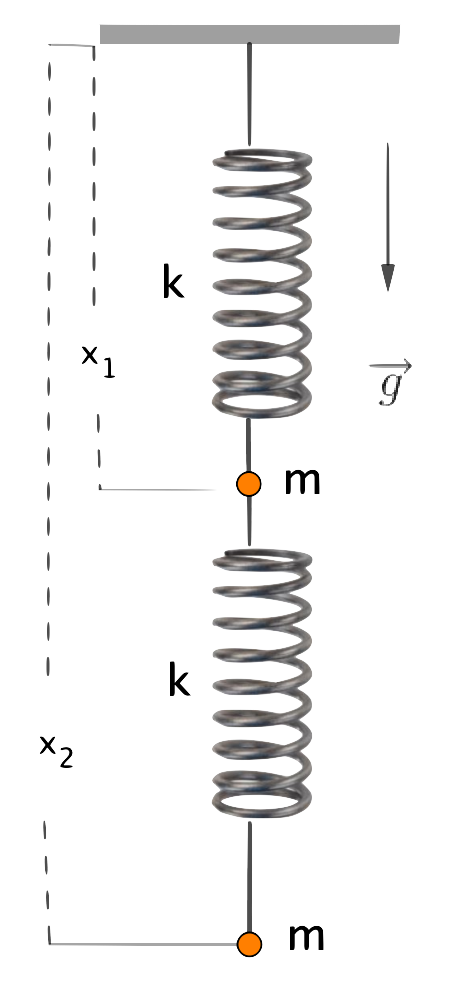
\includegraphics[width=0.15\textwidth]{imagenes/img06-04.png}
	\end{figure}
\end{multicols}
\end{adjustwidth}	
\end{ejercicio}

\vspace{5mm}

\color{MidnightBlue}

No hay fuerzas externas aplicadas y el movimiento se produce un una dirección. Las variables que definen las posiciones de las masas son $x_1 \text{ y } x_2$.	

$T=\dfrac m 2 \ (\dot x_1^2+\dot x_2^2)\ ;\qquad V=\dfrac k 2 \ [\ (x_1-a)^2+(x_2-x_1-a)^2 \ ] \  - \ \ mg\ (x_1+x_2)$

Lagrangiano: 
$\subrayado{ \quad \boldsymbol{L= \dfrac m 2 \ (\dot x_1^2+\dot x_2^2) - \dfrac k 2 \ [\ (x_1-a)^2+(x_2-x_1-a)^2 \ ] \  + \ \ mg\ (x_1+x_2)} }$


\vspace{5mm}
--- Primer cambio de variable \begin{small}(eliminamos la molesta `$a$' de la parte elástica del potencial)\end{small}:

$\begin{cases}
\ x_1 = a+y_1 & \quad \to \quad \dot x_1=\dot y_1 \\
\ x_2 = 2a+y_2 & \quad \to \quad \dot x_2=\dot y_2	
\end{cases}$


Lagrangiano: $\subrayado{ \quad \boldsymbol {L=\dfrac m 2 \ (\dot y_1^2 + \dot y_2^2) \ - \ \dfrac k 2 \ [\ y_1^2 + (y_2-y_1)^2 \ ] \ + \ mg\ (y_1+y_2+3a)} }$

Desarrollando la parte elástica del potencial,

$\quad L=\dfrac K 2 \ (\dot y_1^2 + \dot y_2^2) \ - \ \dfrac k 2 \ [\ 2y_1^2 + y_2^2 -2\ \boldsymbol{y_1\, y_2} \ ] \ - \ mg \ (y_1+y_2+3a)$


Hemos obtenido un lagrangiano acoplado (con las variables $y_1 \text{ e } y_2$ acopladas, término $-2\ y_1\, y_2$). Para desacoplar el problema vamos a \emph{\textbf{diagonalizar}} el problema: aparecerá el segundo cambio de variable.

\vspace{5mm}


$(*)\ \  2y_1^2 + y_2^2 -2 y_1 y_2 = \mqty(y_1&y_2) \ \mqty(2&-1\\-1&1) \ \mqty(y_1\\y_2)=(\vec y)^T \ A \ \vec y \qquad $ \textbf{Diagonalización} de A:

$A\vec v = \lambda \vec v  \ \to \ |A-\lambda I|=\left| \begin{matrix} 2-\lambda & -1 \\ -1 & 1-\lambda \end{matrix} \right| =\lambda^2-3\lambda+1=0 \ \to \ \lambda=\dfrac {3\pm \sqrt{5}}{2}$

\textbf{Valores propios:} $\quad \boldsymbol{\lambda_1=\dfrac {3 + \sqrt{5}}{2}\, M; \quad \lambda_2=\dfrac {3 - \sqrt{5}}{2}}$

Vamos a buscar los \emph{vectores propios} correspondientes:

$\boxed{\ \lambda_1=\dfrac {3 + \sqrt{5}}{2}  \  }\quad$ 

$\mqty[2-\dfrac {3 + \sqrt{5}}{2}&-1\\-1&1-\dfrac {3 + \sqrt{5}}{2}]\ \mqty(x\\y) \ = \ \mqty(0\\0)  \ \to \
\begin{cases} 
\ \dfrac{1-\sqrt{5}}{2}	x-y &=0 \\ \ -x-\dfrac{1+\sqrt{5}}{2}y&=0
\end{cases} 
\to \begin{cases} \ x=1 \\ \  y=\dfrac{1-\sqrt{5}}{2} \end{cases}$

Normalizando: $\ \ |\vec c_1|=\sqrt{1^2+\left( \dfrac{-1+\sqrt{5}}{2} \right)^2 } =\sqrt{\dfrac{5-\sqrt{5}}{2}} \ \ \to \quad 
\boxed{\ \vec c \ = \ \sqrt{\dfrac{2}{5-\sqrt{5}}} \ \mqty(1 \\ \dfrac{1-\sqrt{5}}{2}) \ }$

\rule{200pt}{0.1pt}

$\boxed{\ \lambda_1=\dfrac {3 - \sqrt{5}}{2}  \  }\quad$ 

$\mqty[2-\dfrac {3 - \sqrt{5}}{2}&-1\\-1&1-\dfrac {3 - \sqrt{5}}{2}]\ \mqty(x\\y) \ = \ \mqty(0\\0)  \ \to \
\begin{cases} 
\ \dfrac{1+\sqrt{5}}{2}	x-y &=0 \\ \ -x+\dfrac{-1+\sqrt{5}}{2}y&=0
\end{cases} 
\to \begin{cases} \ x=1 \\ \  y=\dfrac{1+\sqrt{5}}{2} \end{cases}$

Normalizando: $\ \ |\vec c_1|=\sqrt{1^2+\left( \dfrac{1+\sqrt{5}}{2} \right)^2 } =\sqrt{\dfrac{5+\sqrt{5}}{2}} \ \ \to \quad 
\boxed{\ \vec c \ = \ \sqrt{\dfrac{2}{5+\sqrt{5}}} \ \mqty(1 \\ \dfrac{1+\sqrt{5}}{2}) \ }$

\vspace{5mm}

--- Segundo cambio de base (variable):  la matriz $ \ M=\mqty(\vec c_1 & \vec c_2) \ $ del cambio de base $\ \{ y_i \}\ †o \ \{ z_i\} \ $ es (racionalizando\footnote{ Ver al final}):

\hspace{2cm} $M \ = \ \mqty( \sqrt{\dfrac{5+\sqrt{5}}{10}}  &  \sqrt{\dfrac{5-\sqrt{5}}{10}} \\ -\sqrt{\dfrac{5-\sqrt{5}}{10}}  &  \sqrt{\dfrac{5+\sqrt{5}}{10}} )$

y la matriz diagonalizada (matiz de vectores propios) es:

\hspace{2cm} $D\ = \ \mqty(\dfrac{3+\sqrt{5}}{2}&0\\0&\dfrac{3-\sqrt{5}}{2})$

El segundo cambio de variable da lugar a $\ \vec y = M \  \vec z$: 

$\subrayado{
\boxed{ \ \boldsymbol{ \mqty(y_1\\y_2)=\mqty( \sqrt{\dfrac{5+\sqrt{5}}{10}}  &  \sqrt{\dfrac{5-\sqrt{5}}{10}} \\ -\sqrt{\dfrac{5-\sqrt{5}}{10}}  &  \sqrt{\dfrac{5+\sqrt{5}}{10}} ) \mqty(z_1 \\ z_2)
\ \to \ 
\begin{cases}
\ y_1 = \sqrt{\dfrac{5+\sqrt{5}}{10}} z_1 + \sqrt{\dfrac{5-\sqrt{5}}{10}} z_2 \\ \ y_2=-\sqrt{\dfrac{5-\sqrt{5}}{10}}z_1+\sqrt{\dfrac{5+\sqrt{5}}{10}}z_2
\end{cases} } \ } }$

Si sustituimos el la parte variable del potencial elástico (*), obtendríamos:

$ 2y_1^2 + y_2^2 -2 y_1 y_2 = \dfrac {3 + \sqrt{5}}{2} z_1^2 + \dfrac {3 - \sqrt{5}}{2} z_2^2\, , \  $ \begin{small} con lo que las nuevas variables $z_1 \text{ y } z_2$ ya aparecen \emph{desacopladas}\end{small}. 

El lagrangiano es, finalmente:


\begin{equation*} 
\subrayado{
\boxed{\ 
\begin{split}
\boldsymbol{
L } & \boldsymbol{ = \ \dfrac m 2 \ [\  \dot z_1^2 + \dot z_2^2 \ ] \ - \ 
\dfrac k 2 \ \left[ \ \dfrac {3 + \sqrt{5}}{2} z_1^2 + \dfrac {3 - \sqrt{5}}{2} z_2^2 \ 
\right] \ + \ }
 \\
 &  \boldsymbol{+\ mg\ \left[ \ \left(  \sqrt{\dfrac{5+\sqrt{5}}{10}} -  \sqrt{\dfrac{5-\sqrt{5}}{10}} \right) \ z_1 \ + \ \left(  \sqrt{\dfrac{5+\sqrt{5}}{10}} \ + \  \sqrt{\dfrac{5-\sqrt{5}}{10}} \right) \ z_2  \ + \ 3a \ \right] } 
\end{split}
\ }
}
\end{equation*}

\vspace{5mm}

Vamos a obtener las ecuaciones del movimiento, aplicamos \textbf{Euler-Lagrange} para $z_1 \text{ y } z_2$:

$\boxed{\ z_1 \ } \qquad \displaystyle \dv{t}\left[ \pdv{L}{\dot z_1} \right] \ - \ \pdv{L}{z_1} \ = \ 0$

\begin{small}$\displaystyle \dv{t} (m\dot z_1) - k \dfrac{3+\sqrt{5}}{2} z_1 +mg \left(  \sqrt{\dfrac{5+\sqrt{5}}{10}} -  \sqrt{\dfrac{5-\sqrt{5}}{10}} \right)=
m\ddot z_1 - k \dfrac{3+\sqrt{5}}{2} z_1 +mg \left(  \sqrt{\dfrac{5+\sqrt{5}}{10}} -  \sqrt{\dfrac{5-\sqrt{5}}{10}} \right)=0$\end{small}


$\boxed{\ z_2 \ } \qquad \displaystyle \dv{t}\left[ \pdv{L}{\dot z_2} \right] \ - \ \pdv{L}{z_2} \ = \ 0$

\begin{small}$\displaystyle \dv{t} (m\dot z_2) - k \dfrac{3-\sqrt{5}}{2} z_2 +mg \left(  \sqrt{\dfrac{5+\sqrt{5}}{10}} +  \sqrt{\dfrac{5-\sqrt{5}}{10}} \right)=
m\ddot z_2 - k \dfrac{3-\sqrt{5}}{2} z_1 +mg \left(  \sqrt{\dfrac{5+\sqrt{5}}{10}} +  \sqrt{\dfrac{5-\sqrt{5}}{10}} \right)=0$\end{small}

Las \textbf{ecuaciones del movimiento} son: 


\begin{equation*} 
\subrayado{
\boxed{\ 
\begin{split}
\boldsymbol{m\ddot z_1 - k \dfrac{3+\sqrt{5}}{2} z_1 +mg \left(  \sqrt{\dfrac{5+\sqrt{5}}{10}} -  \sqrt{\dfrac{5-\sqrt{5}}{10}} \right)=0}
\\
\boldsymbol{m\ddot z_2 - k \dfrac{3-\sqrt{5}}{2} z_1 +mg \left(  \sqrt{\dfrac{5+\sqrt{5}}{10}} +  \sqrt{\dfrac{5-\sqrt{5}}{10}} \right)=0}
\end{split}
\ } }
\end{equation*}

\vspace{5mm} \textbf{Resolución del sistema} de EDOs segundo orden lineales generales, no homogéneas. Para resolverlas, vamos a escribirlas de modo más sencillo:

$\begin{cases}
\ \subrayado{\boldsymbol{\ddot z_1 - \omega_1^2 z_1 = - K_1}} \, ; \qquad \text{con} \quad \omega_1=\sqrt{\dfrac k m \dfrac{3+\sqrt{5}}{2}} \, ; \qquad  K_1=g\left( \sqrt{\dfrac{5+\sqrt{5}}{10}} - \sqrt{\dfrac{5-\sqrt{5}}{10}} \right)
\\
\ \subrayado{\boldsymbol{\ddot z_2 - \omega_2^2 z_2 = - K_2}} \, ; \qquad \text{con}  \quad \omega_2=\sqrt{\dfrac k m \dfrac{3-\sqrt{5}}{2}} \, ; \qquad  K_2=g\left( \sqrt{\dfrac{5+\sqrt{5}}{10}} + \sqrt{\dfrac{5-\sqrt{5}}{10}} \right)
\end{cases}$

Resolvamos la EDO general para $\boxed{ \ \boldsymbol {z_1} \ }$

\underline{EDO homogénea}: $\ddot z_1-\omega_1^2z_1=0 \to \ \lambda^2-\omega_1^2=0 \to \lambda=\pm \omega_1$

$z_1=ae^{i\omega_1 t}+be^{-i\omega_1 t}=a(cos \omega_1 t + i \sin \omega_1 t)+ b((\cos \omega_1t-i\sin \omega_1 t)=A\cos \omega_1 t + i B \sin \omega_1 t $, escribiendo senos en función de cosenos y dejando las constantes como una fase inicial $D$, podemos decir que la solución general es:$\ {z_1}_g= C \cos(\omega_1 + D)$ \textcolor{gris}{ $\quad (A=a+b, \ B=a-b)$}

\underline{EDO general}:  Como el término independiente de la EDO es una constante, $-K_1$, proponemos como solución \emph{particular} $\ {z_1}_p=T_1=cte$, con lo que ${\dot z_1}_p={\ddot z_1}_p=0$ y, al sustituir en la EDO general: 

$\ 0-\omega_1^2T_1=-K_1 \to T_1=\dfrac{K_1}{\omega_1^2}=\dfrac{g \left( \sqrt{\dfrac{5+\sqrt{5}}{10}} - \sqrt{\dfrac{5-\sqrt{5}}{10}} \right)}{\dfrac k m \dfrac{3+\sqrt{5}}{2}}$

\underline{Solución para $z_1$}:  $\quad \subrayado{\boldsymbol{ z_1=C \cos (\omega_1t+D) + T_1 }}$

Analogamente, \underline{Solución para $z_2$}:  $\quad \subrayado{\boldsymbol{ z_2=E \cos (\omega_1t+F) + T_2 }}$

con $ T_2=\dfrac{K_2}{\omega_2^2}=\dfrac{g \left( \sqrt{\dfrac{5+\sqrt{5}}{10}} + \sqrt{\dfrac{5-\sqrt{5}}{10}} \right)}{\dfrac k m \dfrac{3-\sqrt{5}}{2}}$

\vspace{5mm} Vamos a deshacer los cambios de variable que hemos efectuado  \textcolor{gris}{($M$ es la matriz de cambio de base)}:

$\mqty(x_1\\x_2)=\mqty(y_1\\y_2)+\mqty(a\\2a) = M \mqty(z_1\\z_2)+\mqty(a\\2a)= \mqty( \sqrt{\dfrac{5+\sqrt{5}}{10}}  &  \sqrt{\dfrac{5-\sqrt{5}}{10}} \\ -\sqrt{\dfrac{5-\sqrt{5}}{10}}  &  \sqrt{\dfrac{5+\sqrt{5}}{10}} ) \mqty(z_1\\z_2)+\mqty(a\\2a)$ 

\begin{equation*}
\begin{split}
\boldsymbol{x_1=\ \ \sqrt{\dfrac{\sqrt{5}+1}{2\sqrt{5}}} \ z_1 \ + \ \sqrt{\dfrac{\sqrt{5}-1}{2\sqrt{5}}} \ z_2 = \ \ Mz_1+Nz_2 + \ a } 
\\
\boldsymbol{x_2=-\sqrt{\dfrac{\sqrt{5}-1}{2\sqrt{5}}}\ z_1 \ + \ \sqrt{\dfrac{\sqrt{5}+1}{2\sqrt{5}}} z_2 = -Nz_1+Mz_2 + 2a } 
\end{split}
\qquad  \qquad \text{con} \quad 
\begin{split}
M=\dfrac{\sqrt{5}+1}{2\sqrt{5}}
\\
N=\dfrac{\sqrt{5}-1}{2\sqrt{5}}
\end{split}
\end{equation*}

Sustituyendo las soluciones encontradas para las variables $z_i$, 

\begin{equation*}
	\begin{split}
		x_1= \ M(C \cos (\omega_1t+D) + T_1)+ \ N(E \cos (\omega_2t+F) + T_2)+ \ a
		\\
		x_2=-N(C \cos (\omega_1t+D) + T_1)+M(E \cos (\omega_2t+F) + T_2)+2a
	\end{split}
\end{equation*}


Reagrupando constantes, 


\textcolor{gris}{$\ (MC=P_1, \ NE=Q_1, \ MA_1+NA_2=R_1; \ \ -NC=P_2, \ ME=Q_2, \ -NA_1+MA_2=R_2)$}


\begin{equation*}
	\boxed{ \ \subrayado {
	\begin{split}
	\boldsymbol{ \subrayado { \ x_1 \ = \ P_1 \cos(\omega_1t+D) \ + \ Q_1 \cos (\omega_2t+F) \ + \ R_1+ \ a  \ }}
	\\	
	\boldsymbol{ \subrayado { \  x_2 \ = \ P_2 \cos(\omega_1t+D) \ + \ Q_2 \cos (\omega_2t+F) \ + \ R_2+2a \ }}
	\end{split}
	} \ } 
\end{equation*}

Aparecen en dos términos de cada ecuación los dos modos normales de oscilación más un tercer término de desplazamiento que tiene en cuenta la colocación de las masas.


\vspace{5mm}
Vamos a estudiar un poco estas ecuaciones\footnote{Problema resuelto por Roger Balsach, 22 de julio de 2019}, comparando con los resultados obtenidos para el caso anterior sin gravedad.  Hay, ahora,  dos diferencias con el ejemplo anterior. La primera es evidentemente la gravedad, y la segunda que estamos forzando que el extremo de uno de los muelles esté siempre quieto. Esta segunda tiene una consecuencia inmediata, y es que hemos perdido el término lineal en $t$. Para simplificar el estudio fijamos las fases $D = F = 0$.

Primero de todo vamos a estudiar el caso $P_i = Q_i = 0$. Entonces las masas están quietas (la posición no depende del tiempo) y la solución es $x_1(t) = a + R_1;\ \  x_2(t) = 2a + R_2$. Esto es exactamente lo que obtendríamos si resolviéramos el problema de estática igualando las fuerzas a $0$. Por otra parte, si ``apagamos'' la gravedad, es decir ponemos $g = 0$ obtenemos el mismo resultado anterior, $x_1=a;\ x_2=2a$.

Cuando conectamos solo un modo de vibración, $\omega_1$, lo que podemos ver es que las dos masas suben y bajan juntas, además, como es de esperar, la masa inferior oscila con mayor amplitud que la superior. La gravedad no juega ningún papel importante aquí, pero el hecho de mantener fijo uno de los extremos es lo que provoca no solo la diferencia de amplitudes sino también que la frecuencia de oscilación es más pequeña que en el caso que se deja oscilar libremente (en ese caso recordemos la frecuencia era $\omega_0$).


En caso de conectar solo el segundo modo de vibración, $\omega_2$, las dos masas suben y bajan en contraposición, cuando una sube la otra baja y viceversa. Además la masa inferior tiene ahora una amplitud más pequeña. De nuevo la gravedad no juega ningún papel, y todos los cambios se deben al hecho de haber fijado un extremo, también en este caso la frecuencia es inferior a la que tendríamos con el extremo libre (en ese caso la frecuencia era $\sqrt{3} \omega_0$
	




%\vspace{10mm}


\color{RoyalBlue}
\begin{center}\rule{250pt}{0.2pt}\end{center}

%\vspace{10mm}
\begin{small}
\underline{Nota 3}: Vamos con la racionalización de denominadores para la obtención de la matriz $M$:

$\dfrac 1{\sqrt{ \dfrac{5 \mp \sqrt{5}}{2}}} = \sqrt{\dfrac{2}{5\mp \sqrt{5}}}= \sqrt{\dfrac{2}{5\mp\sqrt{5}} \ \dfrac{5\pm \sqrt{5}}{5\pm \sqrt{5}}} = \sqrt{\dfrac{\cancel{2} \ (5 \pm \sqrt{5})}{\cancel{2} \cdot 10}} = \sqrt{\dfrac{5 \pm \sqrt{5}}{10}}$

%\vspace{3mm} 
$\dfrac 1{\sqrt{ \dfrac{5 - \sqrt{5}}{2}}} \cdot \dfrac {1-\sqrt{5}}{2} = 
\dfrac{\cancel{\sqrt{2}} (1-\sqrt{5} ) }{\sqrt{5-\sqrt{
5}} \sqrt{2} \cancel{\sqrt{2}}}=\dfrac { 1-\sqrt{5} } {\sqrt 2 \sqrt{5-\sqrt{5}} } \dfrac {\sqrt{5-\sqrt{5}}}{ \sqrt{5-\sqrt{5}}} =\dfrac{-(\sqrt{5}-1) \sqrt{5-\sqrt{5}}}{\sqrt{2} (5-\sqrt{5})}=$

$=\text{\begin{small}(factor común denominador)\end{small}}=\dfrac{- \cancel{(\sqrt{5}-1)} \sqrt{5-\sqrt{5}}}{\sqrt{2} \sqrt{5}\ \cancel{(\sqrt{5}-1)}} = -\sqrt{\dfrac{5-\sqrt{5}}{10}}$


%\vspace{3mm} 
Analogamente, $\ \dfrac 1{\sqrt{ \dfrac{5 + \sqrt{5}}{2}}} \cdot \dfrac {1+\sqrt{5}}{2} = \cdots \ \sqrt{\dfrac{5+\sqrt{5}}{10}}$.
%\vspace{3mm} 
$\qquad$Por lo que  $\boldsymbol{ \ \ M \ = \ \mqty( \sqrt{\dfrac{5+\sqrt{5}}{10}}  &  \sqrt{\dfrac{5-\sqrt{5}}{10}} \\ -\sqrt{\dfrac{5-\sqrt{5}}{10}}  &  \sqrt{\dfrac{5+\sqrt{5}}{10}} ) }$

$\,$
\end{small}

\vspace{-10mm}
\color{RoyalBlue}
\begin{center}\rule{350pt}{0.2pt}\end{center}

\color{black}


%\newpage
%\includepdf[pages=-]{imagenes/ejercicio-tema06.pdf}



\chapter{Potencial generalizado. Campo electromagnético}
\label{T7PotenGener}

	\begin{tikzpicture}
	\fill [left color=red!50, right color=teal!50] (0,0) rectangle (6.5,.1);
	\fill [left color=teal!50, right color=blue!50] (6.5,0) rectangle (11.5,.1);
	\end{tikzpicture}


\vspace{10mm}
\begin{adjustwidth}{50pt}{50pt}
\begin{ejemplo}
	Vamos a introducir el \emph{potencial generalizado} aplicado a la fuerza de Lorentz no relativista, $\ \overrightarrow F  =  q \ (\overrightarrow E + \vec v \times \overrightarrow B)\ $. Nuestro objetivo será la formulación del lagrangiano con un cierto potencial $U(q,\dot q,t)$ que responda a la presencia de campos electromagnéticos. ($U$ no solo dependerá de las posiciones $q$ sino también de la velocidades $\dot q$ y del tiempo $t$).
\end{ejemplo}
\end{adjustwidth}


\section{Potencial generalizado}
\vspace{5mm}

La definición de potencial generalizado va a ser:

\begin{equation}
\label{T7potengener}
U(q,\dot q, t) \quad / \qquad \quad \boldsymbol{ Q_j \ = \ \dv{t} \left[ \pdv{U}{\dot q_j} \right] \ - \ \pdv{U}{q_j} }	
\end{equation}


El potencial generalizado $U$ ha de ser una función tal que una fuerza generalizada $Q_j$ se pueda escribir de este modo (Euler-Lagrange) en función de esta $U$, así, el potencial generalizado dará lugar a la fuerza generalizada.

Veamos un ejemplo:

\begin{example}
	\textbf{\emph{Acoplamiento mínimo}} (mecánica cuántica): un electrón en un átomo de Hidrógeno se encuentra sometido a radiación electromagnética externa. Hablaremos de ello al final del tema.	
\end{example}

\vspace{10mm}
\ul{Inciso-1} $\quad$ \rule{100pt}{0.1pt} $\quad$ \textbf{Regla mnemotécnica para el producto vectorial.}

$\vec a\times \vec b=\vec c \ \to \ 
\begin{cases}
\ c_1=a_2b_3-a_3b_2 \\ \  c_2=a_3b_1-a_1b_3 \\  \ c_3=a_1b_2-a_2b_1 	
\end{cases} \qquad \text{orden: } 1231231\cdots \ ,\ $ 

después del 1 va el 2, después el 3, luego el 1 de nuevo y así. Para la componente 3 del producto vectorial, por ejemplo, después de 3 vuelve el 1 y el 2, por eso aparece $a_1b_2$ y luego, restando, al revés, $a_2b_1$.

\vspace{-5mm}

\begin{flushright}
\rule{300pt}{0.1pt}	
\end{flushright}



Aplicado al producto $\ \vec v \times \overrightarrow B \ = \ 
(v_2B_3-v_3B_2,\ v_3B_1-v_1B_3,\ v_1B_2-v_2B_1)$

Y la fuerza de Lorentz, $\ \overrightarrow F \ = q\ \vec B \times \overrightarrow B \, $:

\begin{equation}
\label{T7Lorentz}
\begin{split}
F_1 = q(E_1+v_2B_3-v_3B_2)	\\
F_2 = q(E_2+v_3B_1-v_1B_3)	\\
F_3 = q(E_3+ v_1B_2-v_2B_1)
\end{split}	
\end{equation}

\vspace{5mm}%10
\ul{Inciso-2} $\quad$ \rule{150pt}{0.1pt} $\quad$ \textbf{Teoremas de Cálculo Vectorial.}

\begin{theorem}
.	\vspace{2mm}

	\textbf{Teorema 1} \hspace{2cm} $\qquad \boldsymbol{ \overrightarrow \nabla \cdot (\overrightarrow \nabla \times \overrightarrow A) = 0 } \, ,\quad \forall \overrightarrow A$ 
	
	\vspace{2mm} \textbf{Teorema 2} \hspace{2cm} $\qquad \boldsymbol{ \overrightarrow \nabla \times (\overrightarrow \nabla \ f) = 0 } \, ,\quad \forall \overrightarrow f$ 
	
	\vspace{3mm} \textcolor{gris}{Th1: La divergencia del rotacional es cero.  \hspace{1cm} Th2: El rotacional del gradiente es cero.}
	
	\vspace{2mm}
\end{theorem}

\vspace{-5mm}
\begin{proof} (Primer teorema).

Llamando $\displaystyle \ \partial_1 = \pdv{x}\, , \ \ \partial_2 = \pdv{y}\, , \ \ \partial_3 = \pdv{z} \, , \ $ podemos escribir

$\overrightarrow \nabla \times \overrightarrow A = (\partial_2A_3-\partial_3A_2 , \ \partial_3A_1-\partial_1A_3 , \ \partial_1A_2 - \partial_2A_1)$

$\overrightarrow \nabla \cdot \overrightarrow \nabla \times \overrightarrow A = 
(\partial_1 , \partial_2 , \partial_3 ) \cdot 
(\partial_2A_3-\partial_3A_2 , \ \partial_3A_1-\partial_1A_3 , \ \partial_1A_2 - \partial_2A_1)=$

$\overrightarrow \nabla \cdot \overrightarrow \nabla \times \overrightarrow A =  \partial_1 (\partial_2A_3-\partial_3A_2 ) + \partial_2 ( \partial_3A_1-\partial_1A_3 ) +\partial_3 (\partial_1A_2 - \partial_2A_1)=$

Teniendo en cuenta el teorema de Schwartz, para funciones derivables con derivada continua podemos intercambiar el orden de las derivadas parciales, por ejemplo, $\partial_1 \partial_2 A_3 = \partial_2 \partial_1 A_3$, tendremos, 

$\overrightarrow \nabla \cdot \overrightarrow \nabla \times \overrightarrow A = \cancel{\partial_1 \partial_2A_3} - \bcancel{\partial_1 \partial_3A_2 } + \underline{\partial_2  \partial_3A_1}- \cancel{\partial_2 \partial_1A_3 } + \bcancel{\partial_3 \partial_1A_2} - \underline{\partial_3  \partial_2A_1}= 0$
	
\end{proof}

\vspace{-13mm}

\begin{flushright}
\rule{300pt}{0.1pt}	
\end{flushright}

\vspace{10mm}

Para nuestro propósito vamos a necesitar 3 de las 4 ecuaciones de Maxwell (la cuarta es necesaria para describir ondas electromagnéticas, pero no es nuestro caso).

\begin{small}\textcolor{gris}{No hay distribución de cargas, $\rho=0 \ \to \ \overrightarrow \nabla \cdot E =0$, hay una onda \emph{em} plana que afecta a nuestra carga q.}\end{small}

\begin{myblock}{Ecuaciones de Maxwell (3/4)}
\begin{Large}
\begin{equation} \boldsymbol{
\overrightarrow \nabla \cdot \overrightarrow E = 0\, ; \quad  \quad \overrightarrow \nabla \cdot \overrightarrow B = 0\, ; \quad  \quad \overrightarrow \nabla \times \overrightarrow E = - \pdv{\overrightarrow B}{t} }
\end{equation}
\end{Large}
\end{myblock}

\vspace{5mm}
\normalsize{Nuestro} \underline{objetivo} va a ser encontrar cuatro cantidades $A_0,\ A_1,\ A_2, \ A_3$ (función) de modo que cuando la derivemos con respecto a $x,y,z,t$ nos proporcione los campos $\overrightarrow E$ y $\overrightarrow B$. A estas cuatro cantidades $A^\mu=(A_0, A_1, A_2, A_3)=(A_0,\  \overrightarrow A)$, que dependen de $x,y,z,t$ forma un \emph{cuadrivector} que llamaremos \textbf{Potencial Vector}, $\boldsymbol{A^\mu}$. A partir de combinaciones de derivadas de $A^\mu$ queremos obtener $\overrightarrow E$ y $\overrightarrow B$.

\vspace{5mm} Como la divergencia del rotacional es cero, $\ \overrightarrow \nabla \cdot (\textcolor{red}{\overrightarrow \nabla \times \overrightarrow A})=0\ $ (teorema-1), si nos fijamos en la segunda de Maxwell, M2, $\ \textcolor{red}{\overrightarrow \nabla \cdot B} =0 \, , \  $ concluimos que debe ocurrir que:

\begin{equation}
\textcolor{red}{\boldsymbol{ \overrightarrow B \ = \ \overrightarrow \nabla \cdot \overrightarrow A }}	
\end{equation}
 
 Falta trabajar con las otras dos ecuaciones de Maxwell, M1 y M3.
 
 Si nos fijamos en M3: $ \qquad \overrightarrow \nabla \times \overrightarrow E = \displaystyle -\pdv{t} \ \textcolor{red}{\overrightarrow B} = -\pdv{t} ( \textcolor{red}{\overrightarrow \nabla \times \overrightarrow A })$
 
 Podemos conmutar la derivación por el teorema de Scwartz,: $\quad \displaystyle - \pdv{t} ( \overrightarrow \nabla \times \overrightarrow A ) = - \overrightarrow \nabla \times \left( \pdv{\overrightarrow A}{t}  \right)$
 
 Pasando a la izquierda, $\quad \displaystyle \overrightarrow \nabla \times E \ + \  \overrightarrow \nabla  \times \left( \pdv{\overrightarrow A}{t}  \right) = 0 \, , \ $ agrupando, $\quad \displaystyle \overrightarrow \nabla \times \left[ \textcolor{blue}{\overrightarrow E + \pdv{\overrightarrow A}{t}} \right]=0$
 
 Por el teorema-2, el rotacional del gradiente es nulo, $\ \overrightarrow  \nabla \times (\textcolor{blue}{\overrightarrow \nabla f})=0 \, ,\ $ deducimos que $\quad \textcolor{blue}{ \overrightarrow E + \displaystyle \pdv{\overrightarrow A}{t} = \overrightarrow \nabla f}$
 
 Despejando, $\quad  \overrightarrow E  = \overrightarrow \nabla f -  \displaystyle \pdv{\overrightarrow A}{t} \, . \ $ Tradicionalmente, se escoge que $\boldsymbol f$ sea la componente $\boldsymbol{A_0}$, cambiada de signo,  del potencial vector (cuadrivector $A^\mu$), con lo que,
 
 \begin{equation}
 \boldsymbol{ \textcolor{blue}{\overrightarrow E \ = \ -\overrightarrow \nabla A_0 -  \displaystyle \pdv{\overrightarrow A}{t}}	 }
 \end{equation}
 
\underline{Objetivo conseguido}, ya tenemos $\overrightarrow E \text{ y } \overrightarrow B$ expresados como derivadas del potencial vector $A^\mu$. Ahora vamos a buscar la expresión para el \emph{potencial generalizado} $\boldsymbol{U}$, definido por la ecuación \ref{T7potengener}.

\begin{myalertblock}{Potencial vector}
\begin{large}
\begin{equation}
\boldsymbol{ \overrightarrow B \ = \ \overrightarrow \nabla \cdot \overrightarrow A }
	\qquad \qquad \qquad 
	\boldsymbol{\overrightarrow E \ = \ -\overrightarrow \nabla A_0 -  \displaystyle \pdv{\overrightarrow A}{t}}	 
\end{equation}
\end{large}
\end{myalertblock}

\vspace{5mm}
Si elegimos como coordenadas generalizadas las cartesianas, $q_1=x;\ q_2=y;\ q_3=z$, la definición de fuerza generalizada queda como:

$Q_1=\overrightarrow F \cdot \displaystyle \pdv{\vec r}{q_1}=\overrightarrow F \cdot \displaystyle \pdv{\vec r}{x}=\overrightarrow F \cdot \displaystyle \pdv{(x,y,z)}{x}=\overrightarrow F \cdot (1,0,0)=F_1;\qquad Q_2=F_2;\quad Q_3=F_3$

Como en cartesianas, $Q_j=F_j=\displaystyle \dv{t} \left( \pdv{U}{\dot q_j} \right) + \pdv{U}{q_j}=\dv{t} \left( \pdv{U}{v_j} \right) + \pdv{U}{x_j}$

En las ecuaciones \ref{T7Lorentz} tenemos $\ F \ \sim \ E + vB-Bv$ y debemos encontrar algo como $F\  \sim \ \displaystyle \dv{t} \left(\pdv{v_x}\right) - \pdv{x}\, . \ $Este es el motivo por el que hemos expresado los campos $\overrightarrow E \text{ y } \overrightarrow B$ como combinaciones de derivadas del potencial vector $A^\mu$, apara poder asemejar las expresiones y encontrar quien será $U$, el potencial generalizado.

\begin{small} Como $\overrightarrow E = -\overrightarrow \nabla A_0 - \displaystyle \pdv{\overrightarrow A}{t} \ \to \
\begin{cases}
\ E_1 = -\partial_1 A_0 - \partial_0 A_1 \\
\ E_2 = -\partial_2 A_0 - \partial_0 A_2 \\
\ E_2 = -\partial_2 A_0 - \partial_0 A_3 \\	
\end{cases}$ y también, 
$\overrightarrow B = \overrightarrow \nabla \times \overrightarrow A \ \to \
\begin{cases}
\ B_1= \partial_2 A_3 - \partial_3 A_2 \\	
\ B_2= \partial_3 A_1 - \partial_1 A_3 \\
\ B_3= \partial_1 A_2 - \partial_2 A_1 \\
\end{cases}$ \end{small}

\normalsize{Llevando} estos resultados a las ecuaciones de la fuerza de Lorentz, ec. \ref{T7Lorentz},

\begin{equation}
\label{T7LorentzPotenVector}	
\begin{cases}
\ F_1\ =\ q\ [\ -\partial_1 A_0 - \partial_0 A_1 \ +\  v_2(\partial_1 A_2 - \partial_2 A_1) - v_3(\partial_3 A_1 - \partial_1 A_3) \ ]	\\
\ F_2\ =\ q\ [\ -\partial_2 A_0 - \partial_0 A_2 \ +\  v_3(\partial_2 A_3 - \partial_3 A_2) - v_1(\partial_1 A_2 - \partial_2 A_1) \ ]	\\
\ F_3\ =\ q\ [\ -\partial_3 A_0 - \partial_0 A_3 \ +\  v_1(\partial_3 A_1 - \partial_1 A_3) - v_2(\partial_2 A_3 - \partial_3 A_2) \ ]	
\end{cases}
\end{equation}

Ya tenemos expresada la fuerza (generalizada) $\overrightarrow F$ en función del cuadrivector y de las velocidades. Seguimos buscando la semejanza con
	la ecuación \ref{T7potengener} (en cartesianas) para encontrar el potencial generalizado $U$.
	
El \textbf{truco} a usar es:
	
$ \displaystyle \dv{\overrightarrow A}{t} = \dv{\overrightarrow A(x,y,z)}{t}= 
\pdv{\overrightarrow A}{x} \ \cancelto{ v_x}{\dv{x}{t}}+
\pdv{\overrightarrow A}{y} \ \cancelto{ v_y}{\dv{y}{t}}+
\pdv{\overrightarrow A}{z} \ \cancelto{ v_z}{\dv{x}{z}} 
+ \pdv{\overrightarrow A}{t} =
v_1\partial_1 \overrightarrow A + v_2\partial_2 \overrightarrow A +v_3\partial_3 \overrightarrow A  \ + \ \partial_0 \overrightarrow A$

Leyendo componente a componente esta ecuación: $\ \  \displaystyle \dv{\ A_i \ }{t}=v_1\partial_1 \ A_i + v_2\partial_2 \ A_i + v_3\partial_3 \ A_i+\partial_0 \ A_i$

El último término, $\partial_0 A_i$, aparece en las ecuaciones \ref{T7LorentzPotenVector}, lo despejamos de aquí y lo sustituimos en ellas.

$\displaystyle \partial_0 \ A_i =
 \dv{\ A_i \ }{t} \ - \ \left[v_1\partial_1 \ A_i + v_2\partial_2 \ A_i + v_3\partial_3 \ A_i \right] =  \dv{\ A_i \ }{t} \ - \ (\vec v \cdot \overrightarrow \nabla) \ A_i= \dot A_1  \ - \ (\vec v \cdot \overrightarrow \nabla) \ A_i$
 
 El operador $(v_i\partial 1, \ v_2 \partial_2,\ v_3\partial_3 )=\vec v \cdot \overrightarrow \nabla \, , \ $  se llama \textbf{derivada convectiva}.

Sustituyendo en las ecuaciones \ref{T7LorentzPotenVector},

$\begin{cases}
\ \dfrac{F_1}{q} \ =\ -\partial_1A_0\ - \ [\dot A_1 - (\vec v \cdot \overrightarrow \nabla ) A_1 ] \ + \ [\ v_2(\partial_1 A_2 - \partial_2 A_1) - v_3(\partial_3 A_1 - \partial_1 A_3) \ ]	\\
\ \dfrac{F_2}{q} \ = \ -\partial_2A_0\ - \ [\dot A_2 - (\vec v \cdot \overrightarrow \nabla ) A_2 ] \ + \ [\ v_3(\partial_2 A_3 - \partial_3 A_2) - v_1(\partial_1 A_2 - \partial_2 A_1) \ ]	\\
\ \dfrac{F_3}{q} \ = \ -\partial_3A_0\ - \ [\dot A_3 - (\vec v \cdot \overrightarrow \nabla ) A_3 ] \ + \ 
\ [\  v_1(\partial_3 A_1 - \partial_1 A_3) - v_2(\partial_2 A_3 - \partial_3 A_2) \ ]	
\end{cases}$

Pasando las $\dot A-i$ a la izquierda,

$\begin{cases}
\ \dfrac{F_1}{q} + \ \dot A_1 \ =\ -\partial_1A_0\ + \  (\vec v \cdot \overrightarrow \nabla ) A_1  \ + \ [\ v_2(\partial_1 A_2 - \textcolor{red}{\partial_2 A_1)} - v_3(\textcolor{blue}{\partial_3 A_1} - \partial_1 A_3) \ ]	\\
\ \dfrac{F_2}{q}+ \ \dot A_2 \ = \ -\partial_2A_0\ +\  (\vec v \cdot \overrightarrow \nabla ) A_2  \ + \ [\ v_3(\partial_2 A_3 - \textcolor{red}{\partial_3 A_2)} - v_1(\textcolor{blue}{\partial_1 A_2} - \partial_2 A_1) \ ]	\\
\ \dfrac{F_3}{q}+ \ \dot A_3 \ = \ -\partial_3A_0\ +\  (\vec v \cdot \overrightarrow \nabla ) A_3  \ +  \ [\  v_1(\partial_3 A_1 - \textcolor{red}{\partial_1 A_3)} - v_2(\textcolor{blue}{\partial_2 A_3} - \partial_3 A_2) \ ]	
\end{cases}$

Ya casi lo tenemos.  Fijémonos, por ejemplo, en la primera de las ecuaciones anteriores,


$\dfrac{F_1}{q} + \ \dot A_1 \ =\ -\partial_1A_0\ + \  \textcolor{teal}{( v_1\partial_1 A_1 + \cancel{v_2 \partial_2 A_1} + \bcancel{ v_3 \partial_3 A_1 } ) } \ + \ [\ v_2(\partial_1 A_2 - \textcolor{red}{\cancel{\partial_2 A_1})} - v_3(\textcolor{blue}{ \bcancel{\partial_3 A_1 }} - \partial_1 A_3) \ ]$

Ordenando y simplificando,

$\dfrac{F_1}{q} + \ \dot A_1 \ =\ -\partial_1A_0\ + \  v_1\partial_1 A_1  \ + \  v_2\partial_1 A_2 \ +  \ v_3 \partial_1 A_3$

Como $v_1\neq v_1(x) \ \to \ v_1 \partial_1 A_1 = v_1 \displaystyle \dv{x} A_1 = \dv{x} (v_1 A_1 )= \partial_1 v_1 A_1$, por lo que

$\dfrac{F_1}{q} + \ \dot A_1 \ =\ -\partial_1A_0\ + \  \partial_1 (\vec v \cdot \overrightarrow A) = -\partial_1 \ [A_0-\vec v \cdot \overrightarrow A]$


Y lo mismo para las otras dos ecuaciones.

$\begin{cases}
\ \ \dfrac{F_1}{q} + \ \dot A_1 \  = -\partial_1 \ [A_0-\vec v \cdot \overrightarrow A]\\
\ \ \dfrac{F_2}{q} + \ \dot A_2 \  = -\partial_3 \ [A_0-\vec v \cdot \overrightarrow A] \\
\ \ \dfrac{F_3}{q} + \ \dot A_3 \  = -\partial_3 \ [A_0-\vec v \cdot \overrightarrow A]	
\end{cases}
\textcolor{gris}{\qquad \qquad \sim \qquad \qquad \displaystyle \dv{t}\pdv{U}{v_j}-\pdv{U}{x_j}=F_j}$

Despejando,

$\begin{cases}
\ \ F_1 =  -q\ \dot A_1 - \partial_1 \ \left( q\ [A_0-\vec v \cdot \overrightarrow A] \right) \\	
\ \ F_2 =  -q\ \dot A_2 - \partial_2 \ \left( q\ [A_0-\vec v \cdot \overrightarrow A] \right) \\
\ \ F_3 =  -q\ \dot A_3 - \partial_1 \ \left( q\ [A_0-\vec v \cdot \overrightarrow A] \right) \\
\end{cases}$


Donde, los segundos términos de los segundos miembros de estas ecuaciones se asemejan ya a parte de la ecuación de definición del potencial generalizado, a $\ \displaystyle \pdv{U}{x_j}=\partial_j U$

En los primeros términos del segundo miembro nos falta introducir $\displaystyle \dv{t} \text{ y } \pdv{v_j}$.

Como $\quad -q\dot A_j=\displaystyle \dv{t} (q A_j)$, podemos escribir las ecuaciones anteriores como

$\begin{cases}
\ \ F_1 =  \displaystyle \dv{t} \ (-q A_1) - \partial_1 \ \left( q\ [A_0-\vec v \cdot \overrightarrow A] \right) \\	
\ \ F_2 =  \displaystyle \dv{t} \ (-q A_2) - \partial_2 \ \left( q\ [A_0-\vec v \cdot \overrightarrow A] \right) \\
\ \ F_3 = \displaystyle \dv{t} \ (-q A_3)- \partial_1 \ \left( q\ [A_0-\vec v \cdot \overrightarrow A] \right) \\
\end{cases}$

Fijándonos en los primeros términos (segundos miembros), desearíamos que 

$\ \ \displaystyle  -qA_1 = \pdv{U}{v_i} \ \to \  U=q_1v_1A_1 + cte$, con $cte \neq cte(v_j)$. 

Pero para las otras componentes debe ocurrir lo mismo, $\displaystyle  -qA_2 = \pdv{U}{v_2}\, , \ -qA_3=\pdv{U}{v_3}$, para lo que:

$U\sim cte-qv_1A_1-qv_2A_2-qv_3A_3=cte-q\vec v \cdot \overrightarrow A$

Como $\ A_0 \neq A_0(v_j) \ \to \ U \ = \ q\ A_0 \ -\ q \ \vec v \cdot \overrightarrow A$.

\begin{myblock}{Potencial Generalizado}
\begin{large}
	\begin{equation}
	\begin{small} \text{Conclusión: } \qquad \qquad \qquad \end{small}	\subrayado{\boldsymbol{ \boxed{ \  U \ = \ q\ A_0 \ -\ q \ \vec v \cdot \overrightarrow A \ }}} 	
	\end{equation}
\end{large}	
\end{myblock}

Definiendo el potencial generalizado como $\  U \ = \ q\ A_0 \ -\ q \ \vec v \cdot \overrightarrow A \, , \ $ entonces se cumple la definición del mismo, que $\ \displaystyle \dv{t}\pdv{U}{v_j}-\pdv{U}{x_j}=F_j\, ,$ que es a donde queríamos llegar.

En presencia de campos electromagnéticos, el lagrangiano adopta la forma:


 \begin{myblock}{Lagrangiano con campos em}
\begin{Large}
	\begin{equation}
	\boldsymbol{ \boxed{ \  L\ = \ \dfrac m 2 \ (\dot x^2 + \dot y^2 + \dot z^2) \ -\ \left( qA_0 - q(\vec v \cdot \overrightarrow A )\right) }}	
	\end{equation}
\end{Large}	
\end{myblock}

Quién es $A_\mu$ se ve en electromagnetismo. Con este lagrangiano, nuestra partícula notaría el efecto de un campo \emph{em}, la fuerza de Lorentz.

%\vspace{5mm}

\begin{example}
 
	\begin{multicols}{2}
	\begin{figure}[H]
		\centering
		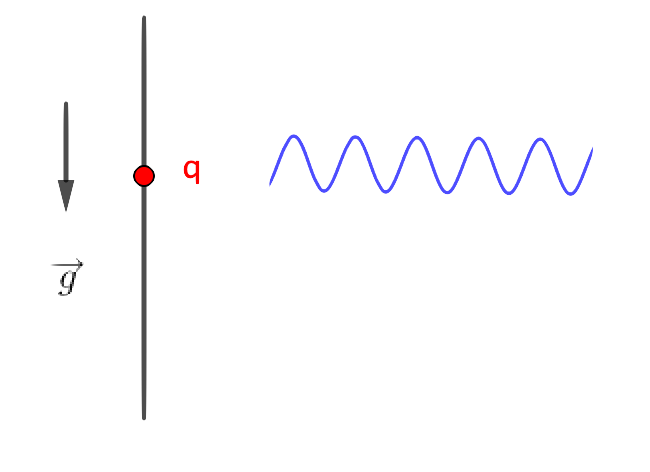
\includegraphics[width=.35\textwidth]{imagenes/img07-01.png}
	\end{figure}
	Partícula $\ q,\ m \ $ que se puede desplazar libremente en una recta, en presencia de la gravedad y ante un campo electromagnético (radiación en forma de onda plana).
	
	El lagrangiano del sistema es:
	
	$$L = \dfrac m 2 \dot z^2 - (qA_o-q\vec v \cdot \overrightarrow A) - mgz$$
	\end{multicols}
\end{example}

Para este tipo de problemas sería más adecuado usar el formalismo \emph{hamiltoniano} que el 	\emph{lagrangiano}. Lo veremos en próximos capítulos.

\subsection{Acoplamento mínimo}

\begin{tikzpicture}
	\fill [left color=red!50, right color=teal!50] (0,0) rectangle (3.5,.01);
	\fill [left color=teal!50, right color=blue!50] (3.5,0) rectangle (7.5,.01);
	\end{tikzpicture}
\vspace{0.5cm}


Supongamos una carga libre en presencia de un campo electromagnético (radiación), solo va a haber fuerza de Lorentz.

En estas ocasiones, lo veremos más adelante (formulación hamiltoniana) pero es conveniente recordarlo, la cantidad de movimiento definida como $\ \vec p = m \vec v \ $ no es la manera adecuada de definirla, hay que usar la forma:

$$\boxed{ \ \boldsymbol{ \overrightarrow {\mathcal P} \ = \ m\vec v \ + \  q\overrightarrow A} \ }$$
\chapter{Principio de \emph{Hamilton}}

	\begin{tikzpicture}
	\fill [left color=red!50, right color=teal!50] (0,0) rectangle (6.5,.1);
	\fill [left color=teal!50, right color=blue!50] (6.5,0) rectangle (11.5,.1);
	\end{tikzpicture}

% \var{S}    \fdv{S}{t}

\vspace{10mm}
\begin{adjustwidth}{50pt}{50pt}
\begin{ejemplo}
	Se enuncia brevemente el \emph{principio de Hamilton, de mínima acción o de acción estacionaria}.
	
	Para más información ver apéndice \ref{ApendiceFuncional} Funcional'.



\end{ejemplo}
\end{adjustwidth}

\section{Principio de \emph{Hamilton}}

\begin{myblock}{Principio de Hamilton, de mínima acción o de  acción estacionaria}
Dado el funcional \emph{\textbf{acción}}	 

$$\boldsymbol{
S\ = \ \displaystyle \int_{t_1}^{t_2} \ L(q_j,\ \dot q_j,\ t) \ \dd t
}$$

\vspace{2mm} el sistema (clásico) evolucionará en el tiempo siguiendo las ecuaciones (opuestas a Euler-Lagrange)

$$\displaystyle \pdv{L}{q_j} \ - \ \dv{t} \left( \pdv{L}{\dot q_j} \right) = 0$$

\vspace{2mm} o, lo que es lo mismo,

$$\subrayado{ \ \boxed{\  \boldsymbol{
\displaystyle \fdv{S}{q_j} \ = \ 0 \quad \leftrightarrow \quad \var S = 0 
} \ } \ }$$

\vspace{2mm} la variación de la acción es cero.
\end{myblock}


\subsection{Derivada funcional}
\label{T8Funcional}
\vspace{-5mm}
\begin{tikzpicture}
	\fill [left color=red!50, right color=teal!50] (0,0) rectangle (3.5,.01);
	\fill [left color=teal!50, right color=blue!50] (3.5,0) rectangle (7.5,.01);
	\end{tikzpicture}
\vspace{1cm}

\begin{myexampleblock}{ ?`Qué es un funcional?}
Basado en los vídeos comentados en el principio del capítulo.	

	
	
\begin{figure}[H]
		\centering
		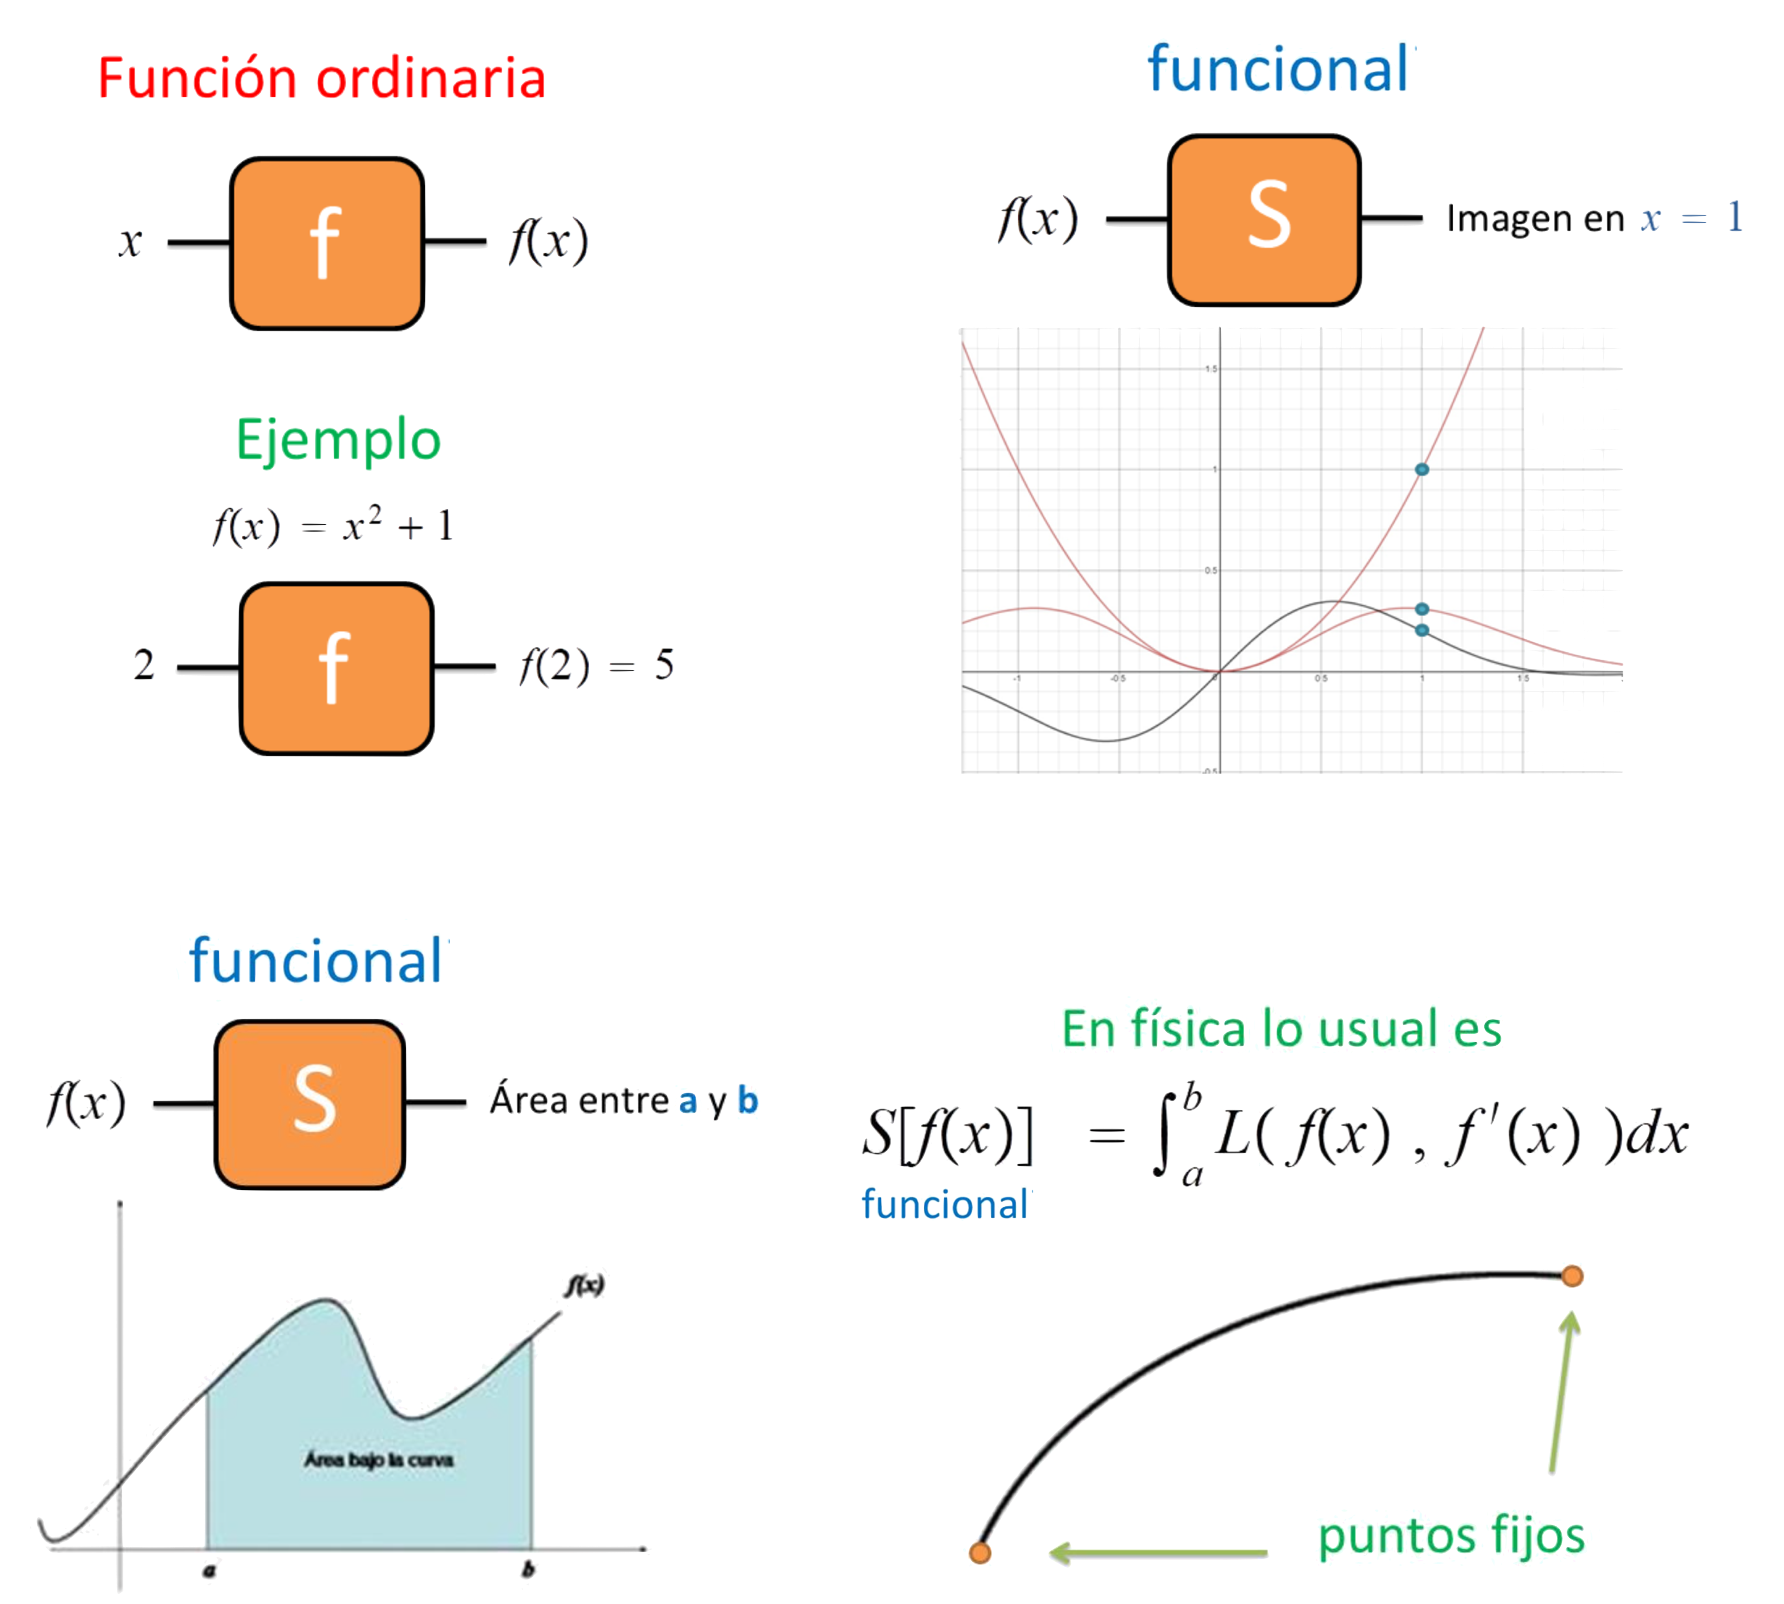
\includegraphics[width=1\textwidth]{imagenes/img08-01.png}
	\end{figure}
	
\begin{center} \rule{200pt}{0.1pt} \end{center}

\begin{figure}[H]
		\centering
		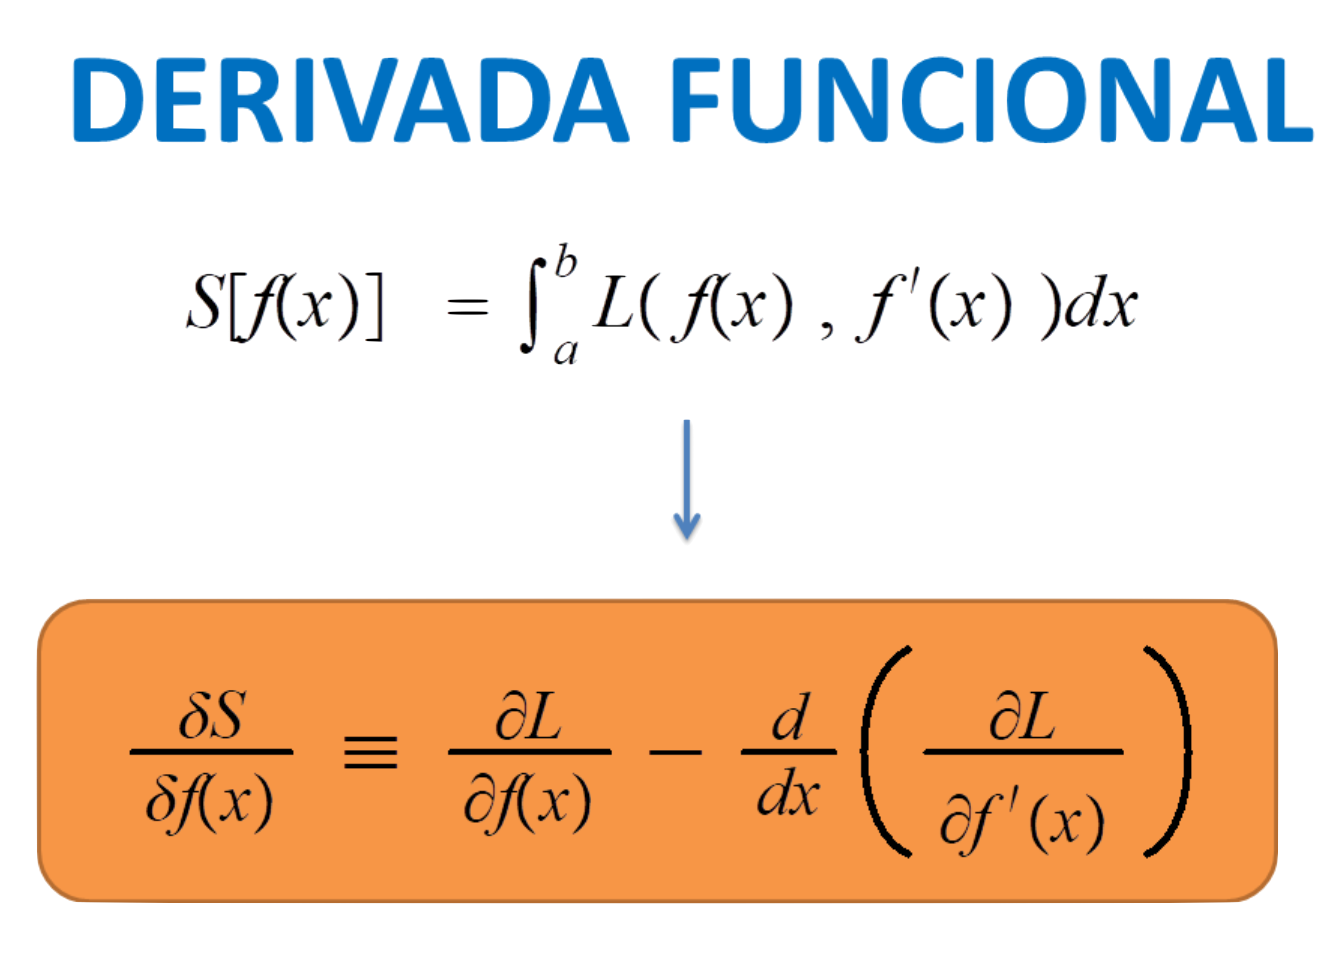
\includegraphics[width=.5\textwidth]{imagenes/img08-02a.png}
	\end{figure}
	
\begin{figure}[H]
		\centering
		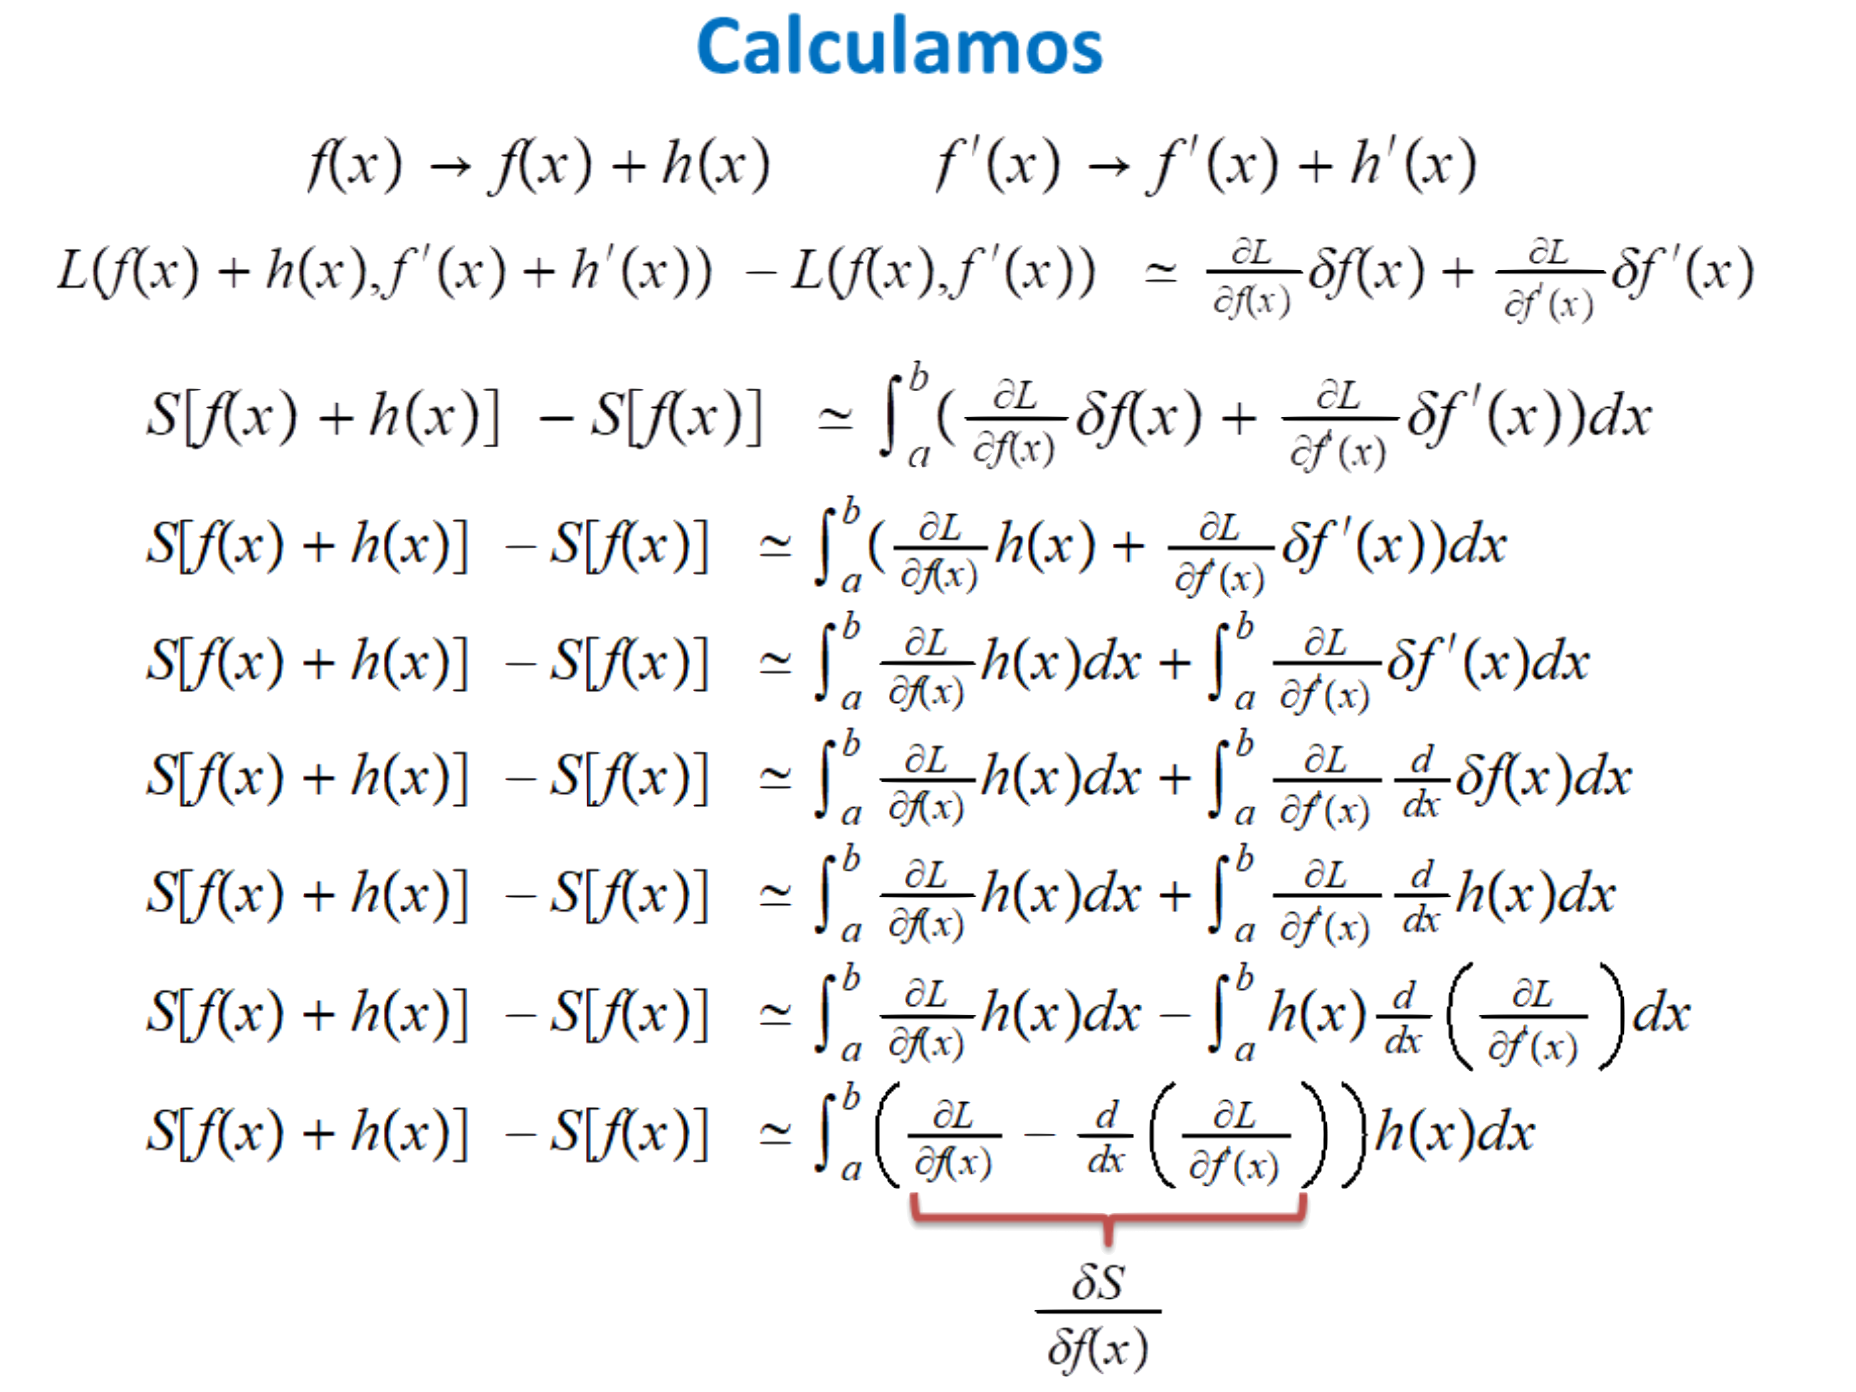
\includegraphics[width=.9\textwidth]{imagenes/img08-02b.png}
	\end{figure}
	
\begin{figure}[H]
		\centering
		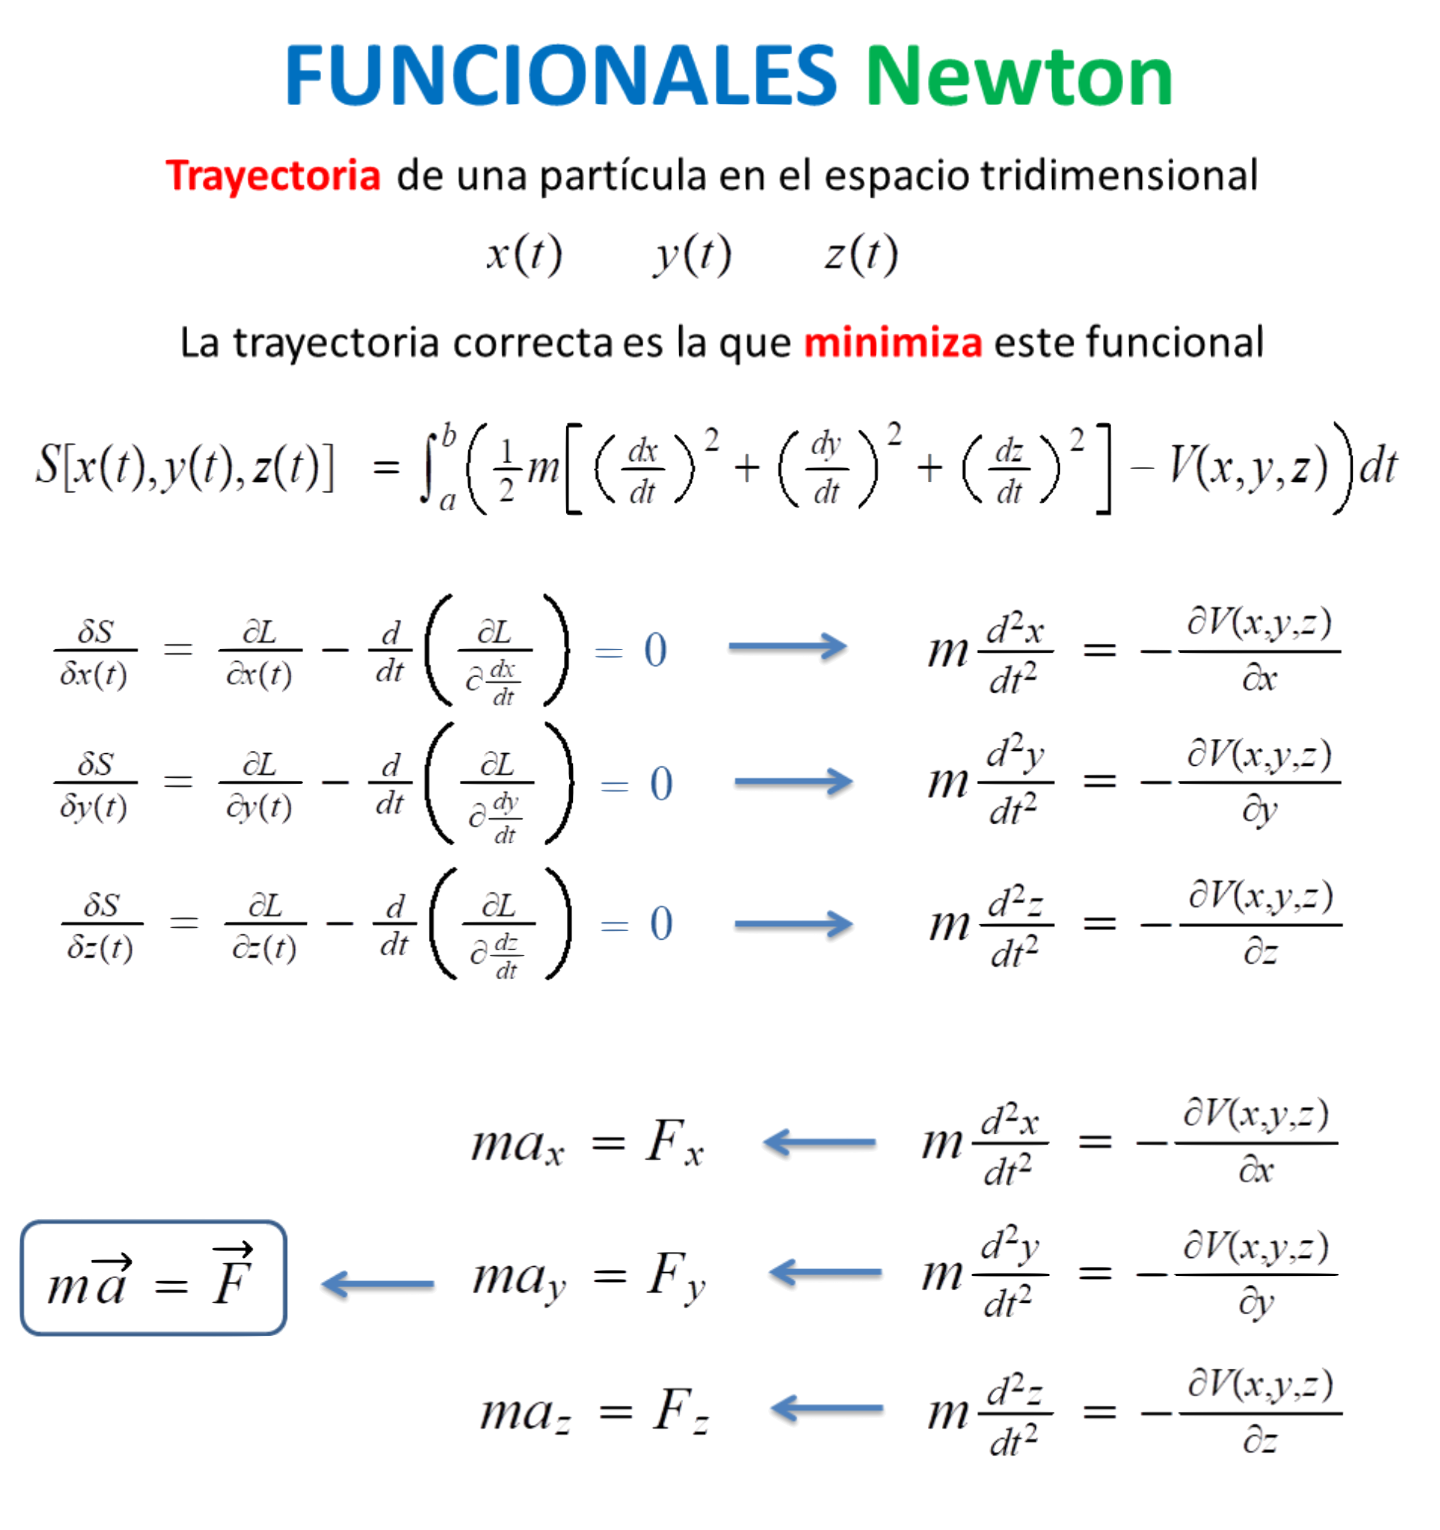
\includegraphics[width=.8\textwidth]{imagenes/img08-03.png}
	\end{figure}

\end{myexampleblock}

\begin{ejemplo}
\vspace{2mm}

Reproduzco, a continuación, el apéndice II de mis apuntes sobre los ``Grupos de Lie'' basados, también, en el video curso de Javier García del mismo nombre. 

\textcolor{teal}{
\begin{footnotesize}
{https://www.youtube.com/playlist?list=PLAnA8FVrBl8DTFTMP8kXbDnRJHQKqfjaw}	
\end{footnotesize} }
\vspace{2mm}
\end{ejemplo}


\newpage
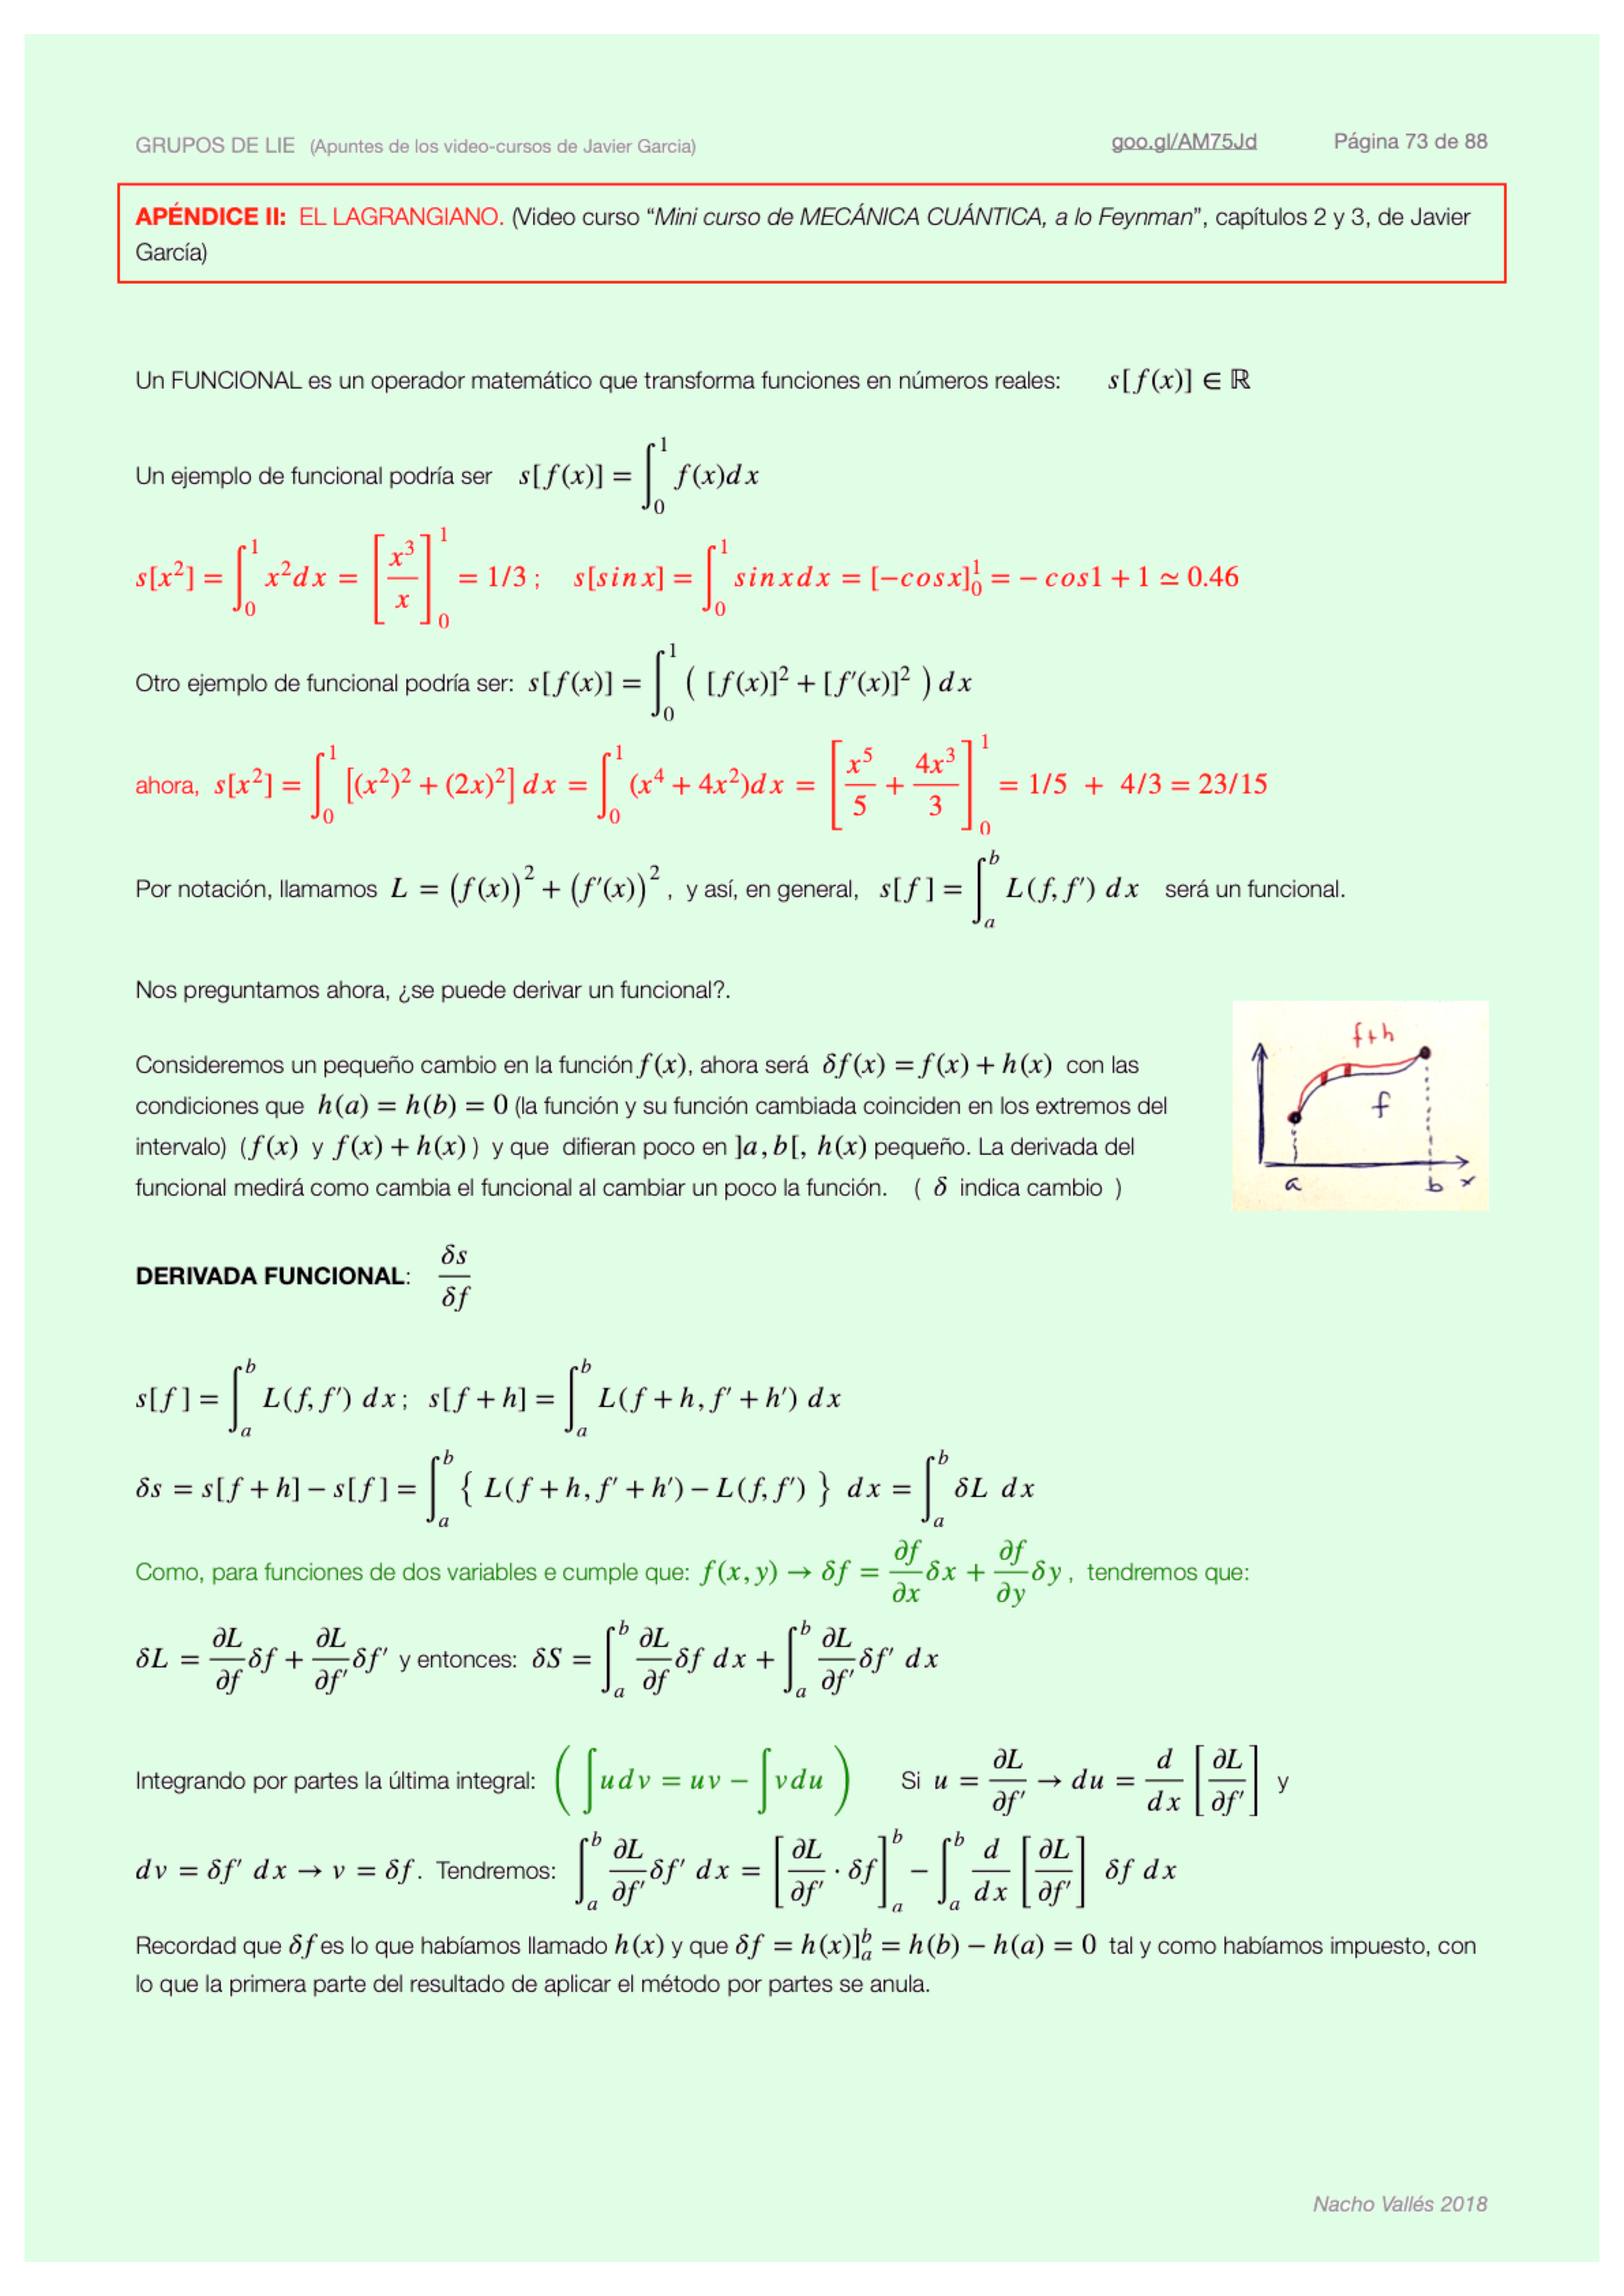
\includepdf[pages=-]{imagenes/derivada-funcional.pdf}






\chapter{Ligaduras no holónomas}

	\begin{tikzpicture}
	\fill [left color=red!50, right color=teal!50] (0,0) rectangle (6.5,.1);
	\fill [left color=teal!50, right color=blue!50] (6.5,0) rectangle (11.5,.1);
	\end{tikzpicture}


\vspace{10mm}
\begin{adjustwidth}{50pt}{50pt}
\begin{ejemplo}
El problema que vamos a resolver es el del movimiento de un robot en la superficie de Marte. El robot podrá girar sobre su CM y se puede desplazar rectilíneamente sobre su eje.

Exigiremos que el robot \emph{no derrape}, que su vector velocidad sea paralela a su eje. Este será nuestro ejemplo (típico) de ligadura no holónoma.

\begin{figure}[H]
		\centering
		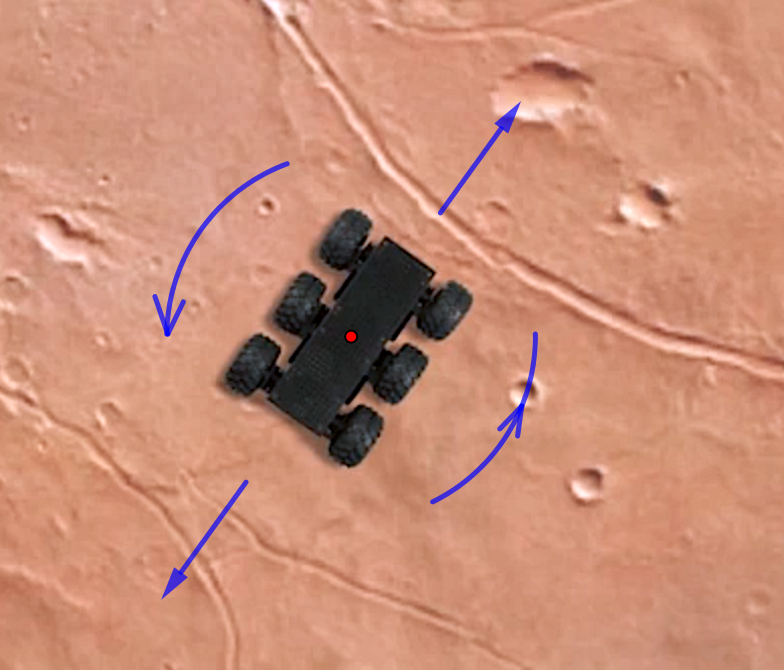
\includegraphics[width=.75\textwidth]{imagenes/img09-01.png}
	\end{figure}

\vspace{2mm}
\end{ejemplo}
\end{adjustwidth}

\begin{myblock}{Principio de Hamilton}

\begin{large}
\begin{equation}
\boldsymbol{
S\ = \ \displaystyle \int_{t_1}^{t_2} \ L(q_j,\ \dot q_j,\ t) \ \dd t 
\quad \quad \to \quad \quad \var S\ = \ 0
}
\end{equation}
\end{large}
\end{myblock}


\section{Ligaduras no holónomas}

Hasta ahora solo hemos visto \emph{ligaduras holónomas}, en que podemos expresar las coordenadas de las partículas en función de las coordenadas generalizadas y del tiempo, $\ \vec r=\vec r(q_i,t)\, . \ $ Cuando esto no es posible, decimos que las ligaduras son \emph{\textbf{no holónomas}}.

Por motivos de claridad en la exposición, consideraremos que solo tenemos dos coordenadas generalizadas, $\ q_1 \text{ y } q_2$ (la extensión a mayor número de variables generalizadas es trivial).

En las ligaduras \emph{no holónomas} se imponen condiciones del tipo:

\begin{equation}
\label{T9Def1LNH}
\mqty(\xmat*{a}{2}{2}) \ \mqty(\dot q_1 \\ \dot q_2)  \ = \ - \mqty(a_{10}\\a_{20})
\end{equation}

\textcolor{gris}{(encontraremos sentido a este modo de imponer ligaduras cuando abordemos el problema del robot en Marte).}

De otro modo, $\qquad  \displaystyle \ \mqty(\xmat*{a}{2}{2}) \ \mqty(\dv{t} q_1 \\ \dv{t} q_2)  \ = \ - \mqty(a_{10}\\a_{20})\, , \ $ despejando

\begin{equation}
\label{T9LNH}
\mqty(\xmat*{a}{2}{2}) \ \mqty(\dd q_1 \\ \dd q_2)  \ = \ - \mqty(a_{10}\\a_{20}) \ \dd t
\end{equation}

Ambas maneras de expresar las ligaduras no holónomas son equivalentes.

Recordemos que un \emph{desplazamiento virtual} ocurre cuando el tiempo está fijo (congelado):  $\qquad $  $\qquad $ $\boldsymbol{\var q \ = \ {(\dd q)}_{\, t\ fijo}}\, , \ $ (ver sección \ref{T1PTV}). Pues bien, para desplazamientos virtuales, si el tiempo es fijo, en la definición de ligaduras no holónomas de las ecuaciones \ref{T9LNH}, $\ \dd t=0 \to $

$\displaystyle  \to \ \mqty(\xmat*{a}{2}{2}) \  \mqty(\var   q_1 \\ \var   q_2) \ = \ M  \  \mqty(\var  q_1 \\ \var  q_2) \ = \  \mqty(0 \\ 0) \, . \ $ 

Si $|M|=0$, tendremos un sistema compatible determinado que, como es homogéneo, tendrá solución única: la trivial, $\var q_1 = \var q_2=0$. No hay movimiento posible en el sistema. Esto es una contradicción, por lo que $|M| \neq 0$, con lo que las filas de la matriz $M$ serán proporcionales, $(a_{11} \ a_{12}) = k (a_{21} \ a_{22})$. Solo quedará una ecuación libre: $\boldsymbol{ \  a_{11} \ \var q_1 \ + \   a_{12} \ \var q_2 \ = \  0\, , \  }$ en el caso 2D (2 coordenadas generalizadas). 

\emph{``Para ligaduras holónomas las variables generalizadas son independientes, en las no holónomas hay relaciones entre ellas''.}

Del principio de Hamilton cuando las ligaduras son holónomas se obtienen las ecuaciones de Euler-Lagrange, $\ \displaystyle \pdv{L}{q_j} - \dv{t} \left( \pdv{L}{\dot q_j} \right)  = 0$. Veamos que ocurre con las ligaduras no holónomas.

$$ \displaystyle \var S = \int_{t_1}^{t_2} \ \left\{ \ \ 
\left[ \pdv{L}{q_1} - \dv{t} \left( \pdv{L}{\dot q_1} \right) \right] \ \var q_1 \ + \ 
\left[ \pdv{L}{q_2} - \dv{t}  \left( \pdv{L}{\dot q_2} \right) \right] \ \var q_2
 \ \right\} \ = \ 0 $$
 
 Como ahora (ligaduras no holónomas) $\var q_1 \text{ y } \var q_2$ no son independientes, no podemos exigir que ambos integrandos sean cero. Despejando de la ecuación libre que relacionaba ambas variables, $\ a_{11} \ \var q_1 \ + \   a_{12} \ \var q_2 \ = \  0 \ \to \ \var q_2 \ = \ -\dfrac {a_{11}}{a_{12}} \ \var q_1 \, , \ $ por lo que
 
 
$\displaystyle \left[ \pdv{L}{q_1} - \dv{t} \left( \pdv{L}{\dot q_1} \right) \right] \ \var q_1 \ - \ 
\left[ \pdv{L}{q_2} - \dv{t} \left( \pdv{L}{\dot q_2} \right) \right] \ \dfrac {a_{11}}{a_{12}} \ \var q_1 \ = \ 0 $

$\displaystyle \left[ \ 
\left[ \pdv{L}{q_1} - \dv{t} \left( \pdv{L}{\dot q_1} \right) \right] \ - \ 
\left[ \pdv{L}{q_2} - \dv{t} \left( \pdv{L}{\dot q_2} \right) \right] \ \dfrac {a_{11}}{a_{12}} \ \right] \ 
 \cancelto{\neq 0}{\var q_1} \ = \ 0  \ \to$
 
 $\displaystyle \ \to \ 
 \left[ \ 
\left[ \pdv{L}{q_1} - \dv{t} \left( \pdv{L}{\dot q_1} \right) \right] \ - \ 
\left[ \pdv{L}{q_2} - \dv{t} \left( \pdv{L}{\dot q_2} \right) \right] \ \dfrac {a_{11}}{a_{12}} \ \right] \ = \ 0$

$$\boldsymbol{
\displaystyle \left[ \pdv{L}{q_1} - \dv{t} \left( \pdv{L}{\dot q_1} \right) \right] \ a_{12} \ = \ 
\left[ \pdv{L}{q_2} - \dv{t} \left( \pdv{L}{\dot q_2} \right) \ \right] \ a_{11}  }$$

Que son las \textbf{ecuaciones de Euler-Lagrange modificadas para el caso de ligaduras no holónomas}.

Para escribir esto más elegantemente vamos a usar el \emph{truco} que se le ocurrió a Lagrange:

\vspace{5mm}
\subsection{Multiplicadores de \emph{Lagrange}}
\begin{tikzpicture}
	\fill [left color=red!50, right color=teal!50] (0,0) rectangle (3.5,.01);
	\fill [left color=teal!50, right color=blue!50] (3.5,0) rectangle (7.5,.01);
	\end{tikzpicture}
\vspace{0.5cm}

Dividiendo la expresión anterior entre $\ a_{11} \ a_{12}\, ,$

$\dfrac{\displaystyle  \left[ \pdv{L}{q_1} - \dv{t} \left( \pdv{L}{\dot q_1} \right) \right]}{a_{11}} \ = \ \dfrac{\displaystyle  \left[ \pdv{L}{q_2} - \dv{t} \left( \pdv{L}{\dot q_2} \right) \ \right]}{a_{12}} \ = \ \boldsymbol{- \lambda}$ \hspace{1cm}\textcolor{gris}{(truco)}

$\displaystyle \pdv{L}{q_1} - \dv{t} \left( \pdv{L}{\dot q_1} \right)  \ = \ -\lambda \ a_{11} 
\qquad \text{ y } \qquad
\pdv{L}{q_2} - \dv{t} \left( \pdv{L}{\dot q_2} \right)  \ = \ -\lambda \ a_{12} $

Multiplicando por $- 1$,

\begin{equation}
	\subrayado{\boxed{ \ \boldsymbol{ 
	\dv{t}\left( \pdv{L}{\dot q_1} \right) - \pdv{L}{q_1}  = \lambda a_{11}
	} \ }}
	\qquad \qquad 
	\subrayado{\boxed{ \ \boldsymbol{ 
	\dv{t}\left( \pdv{L}{\dot q_2} \right) - \pdv{L}{q_2}  = \lambda a_{12}
	} \ }}
\end{equation}
\begin{center} Ecuaciones de Euler-Lagrange para el caso 2D de ligaduras no holónomas. \end{center}

\vspace{1cm}
\begin{myalertblock}{En general}

Ligaduras no holónomas: $\quad \displaystyle \boldsymbol{
\sum_{j=1}^n a_{ij} \dot q_j = -a_{i_0}\, ;\ 
\qquad  
\sum_{j=1}^n a_{ij} \dd q_j = -a_{i0} \dd t \, ;\ 
 }	 \quad i=1,2, \cdots , p$
 
\vspace{5mm} Ecuaciones Euler-Lagrange para ligaduras no holónomas:

\begin{large}
$$\displaystyle \subrayado{ \ \boxed{ \ \boldsymbol{
\dv{t}\left( \pdv{L}{\dot q_j} \right) - \pdv{L}{q_j}  = \sum_{i=1}^p \lambda_i a_{ij}
} \ } \ }$$
\end{large}
 
\end{myalertblock}




\vspace{1cm}
\subsection{Aplicación: problema del robot en Marte}
\label{T4SecELF}
\begin{tikzpicture}
	\fill [left color=red!50, right color=teal!50] (0,0) rectangle (3.5,.01);
	\fill [left color=teal!50, right color=blue!50] (3.5,0) rectangle (7.5,.01);
	\end{tikzpicture}
\vspace{0.5cm}

\begin{example}

\begin{multicols}{2}
\begin{figure}[H]
		\centering
		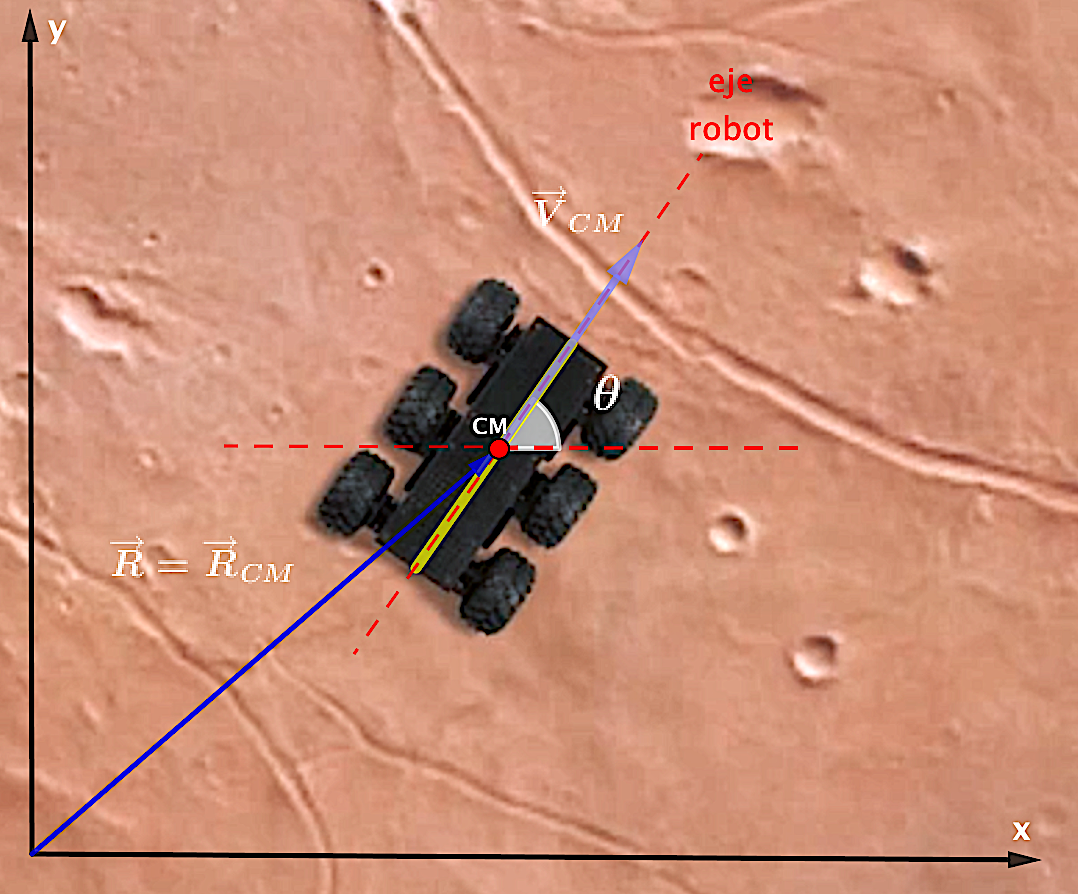
\includegraphics[width=.45\textwidth]{imagenes/img09-02.png}
	\end{figure}	
	
	El robot puede girar sobre su CM y desplazarse según su eje pero sin derrapar (ligadura no holónoma): la velocidad del centro de masas del robot ha de ser paralela a su eje.

\vspace{2mm} Con $\overrightarrow R \text{ y } \theta$ tenemos determinada la posición del robot. 

\vspace{2mm} Si no hubiese ninguna restricción, el lagrangiano del sistema sería (como en la sección \ref{T5ELroracion}).

\begin{equation}
\tag{\ref{T5Lconrotacion}}
L \ = \ \dfrac{M}{2}\ \ V_{CM}^2 \ + \ \dfrac 1 2 \ I_{CM}\  \ \dot \theta^2	
\end{equation}
\end{multicols}

\vspace{2mm} Como $\overrightarrow R(x,y);\ \overrightarrow V(x,y) \ \to \ L=\dfrac M 2 (\dot x^2 + \dot y^2)+\dfrac{I_{cm}}{2} \dot \theta^2$


\vspace{5mm}Imponemos ahora la restricción de la ligadura no holónoma de que el robot no pueda derrapar: $\ \overrightarrow V_{CM} \ || \ $ eje del robot.

\vspace{2mm}$\overrightarrow V=(V_x,V_y)=(V\cos \theta,\, V\sin \theta) \ \to \ \tan \theta=\dfrac {V_y} {V_x} \ \to V_x \tan \theta = V_y \ \to \ V_x \dfrac{\sin \theta}{\cos \theta}=V_y  \to \ V_x\sin \theta  = V_y \cos \theta \ \to \quad  \sin \theta \ \dot x = \cos 	\theta \ \dot y$

\vspace{2mm} En nuestro caso, las variables generalizadas son: $\ q_1=x;\ q_2=y;\ q_3=\theta$

\vspace{2mm}
\begin{equation}
\label{T9EjLNH}
\text{Ligadura no holónoma: } \qquad \boxed{\bold{ \ \sin \theta \ \dot x = \cos 	\theta \ \dot y \ }}
\qquad \qquad \textcolor{gris}{(\sin \theta \ \dot q_1 = \cos 	\theta \ \dot q_2)}
\end{equation}

\vspace{2mm} Identificando con el caso general


\vspace{2mm}
Asimilando esto a la definición de ligaduras no holónomas, ec. \ref{T9Def1LNH}, podemos escribir:

\vspace{2mm} 
$\mqty(\sin \theta & -\cos \theta & 0 \\ 0&0&0 \\ 0&0&0  ) \ \mqty(\dot q_1 \\ \dot q_2 \\ \dot q_3) \ = \ \mqty(0\\0\\0) \qquad $
Identificamos: $\ \  \boldsymbol{a_{11}=\sin \theta\,;\ \ a_{12}=\cos \theta}$

\vspace{2mm} Escribamos las ecuaciones de Euler-Lagrange para el caso de ligaduras no holónomas y para nuestras tres coordenadas generalizadas, $x,\ y,\ \theta$

\vspace{5mm}

Coordenada $\ \boxed{  x  }\,: \quad  \qquad  \displaystyle \dv{t} \left( \pdv{L}{\dot x} \right) - \pdv{L}{x} = \lambda \sin \theta \ \to \ \dv{t} (M\dot x) - 0 = \lambda \sin \theta$

Coordenada $\ \boxed{  y  }\,: \quad  \qquad  \displaystyle \dv{t} \left( \pdv{L}{\dot y} \right) - \pdv{L}{y} = -\lambda \cos \theta \ \to \ \dv{t} (M\dot y) - 0 = -\lambda \cos \theta$

Coordenada $\ \boxed{  \theta  }\,: \quad  \qquad  \displaystyle \dv{t} \left( \pdv{L}{\dot \theta} \right) - \pdv{L}{\theta} = 0 \ \to \ \dv{t} (I_{CM} \dot \theta) \ - \ 0 \  = 0 \ \to \ I_{CM} \ddot \theta =0$

\vspace{2mm}
\begin{equation}
	\label{T9EjEcMov}
	\boldsymbol{
	\begin{cases} 
		\ \ M \ \ddot x \ = \ \  \lambda \ \sin \theta \\
		\ \  M \ \ddot y \ = \ - \lambda \ \cos \theta \\
		\ \ \dot \theta \ = \  \omega  \ \textcolor{gris}{ = \  cte}
	\end{cases} 
	}
\end{equation}


\vspace{2mm} Integrando las ecuaciones diferenciales de movimiento,
$\quad \boxed{ \boldsymbol{\theta=\omega t + \varphi_0} \ }$

\vspace{2mm}Las ecuaciones en $\dot x \text{ y } \dot{y} $ están \emph{acopladas}, pero de la relación de ligadura, ec \ref{T9EjLNH},

\vspace{2mm}$\boldsymbol{\sin \theta \ \dot x = \cos 	\theta \ \dot y}  \ \ \to \ \begin{cases}
 \ \ddot x = \ \dfrac \lambda M \sin \theta	\ \to \ \ \sin \theta = \ \ \dfrac M \lambda \ddot x\\  \\ 
 \ \ddot y = - \dfrac \lambda M \cos \theta \ \to \ \cos \theta = \ - \dfrac M \lambda \ddot y 
 \end{cases}
 \ \to \quad  \boldsymbol{\dfrac M \lambda \ddot x \ \dot x +  \dfrac M \lambda \ddot y \ \dot y =0}$

\vspace{2mm}Simplificando, $\ \ddot x \ \dot x+\ddot y \ \dot y=0$

\vspace{2mm}Como $\displaystyle \dv{t}( \Box ^2) = 2 \ \Box \ \dot{\Box} \ \to \ 
\dv{t}( \dot{\Box}^2 )  =2 \ \dot{\Box} \ \ddot{\Box}$

\vspace{2mm}Luego, $\ 2 \ \ddot x \ \dot x+ 2 \ \ddot y \ \dot y=0 \ \to \ \displaystyle
\dv{t} (\dot x^2) + \dv{t} (\dot y^2) =0 \ \to \ 
\dv{t} (\dot x^2+\dot y^2)=0 \ \to \ 
\boldsymbol{\dot x^2+\dot y^2 = A^2} \ \textcolor{gris}{(=cte)}$
 

\vspace{2mm} Despejando de $\ \sin \theta \ \dot x = \cos 	\theta \ \dot y \ \to \ \dot y=\dfrac{\sin \theta}{\cos \theta} \ \dot x\, $ [ecuación $(^*)$] y sustituyendo en la ecuación que acabamos de encontrar: 

\vspace{2mm} $\dot x^2+\dot y^2 = A^2 \ \to \ \dot x^2+\left( \dfrac{\sin \theta}{\cos \theta} \ \dot x \right)^2 = A^2 \ \to \ 
 x^2 \ \left( 1+ \dfrac{\sin^2 \theta}{\cos^2 \theta} \right) = A^2  \ \to \ \dot x^2 \ \dfrac{1}{\cos^2 \theta} =A^2 $
 
\vspace{2mm} $\dot x^2 = A^2 \ \cos^2 \theta \ \to \ x= A \ \cos \theta\, ,\  $ tercera ecuación de movimiento, $\ \dot x=A\ \cos(\omega t+\varphi_0)$

\vspace{2mm} Integrando, $\quad \boxed{ \ \boldsymbol{x=\dfrac A \omega \ \sin(\omega t + \varphi_0) + B } \ }$

\vspace{2mm} Sustituyendo en [ecuación $(^*)$] $\quad \dot y=\dfrac{\sin \theta}{\cos \theta} \ \left( \dfrac A \omega \ \sin(\omega t + \varphi_0) + B  \right)' = A\ \sin(\omega t + \varphi_0)$

\vspace{2mm} Integrando, $\quad \boxed{ \ \boldsymbol{y=-\dfrac A \omega \ \cos(\omega t + \varphi_0) + C } \ }$


\vspace{2mm} Las ecuaciones (integradas) de movimiento son:

\vspace{2mm} \begin{equation}
 \label{T9EjEcMovoInteg}	
 \subrayado{
 \boxed{ \ \boldsymbol{x=\dfrac A \omega \ \sin(\omega t + \varphi_0) + B } \ }
 \qquad
  \boxed{ \ \boldsymbol{y=-\dfrac A \omega \ \cos(\omega t + \varphi_0) + C } \ }
  \qquad
  \boxed{ \boldsymbol{\theta=\omega t + \varphi_0} \ }
  }
 \end{equation}


\vspace{2mm} También se podría calcular el valor de $\boldsymbol \lambda$, a partir de la expresión $M\ddot x= \lambda \sin \theta \text{ ó } M\ddot y= -\lambda \cos \theta$, pero puede ser fijado con las constantes $A, \ B, \ C,\ \varphi_0$ en las condiciones iniciales del problema.

\vspace{5mm} 
\begin{multicols}{2}
\underline{Sorpresa}: Las ecuaciones $ x=\dfrac A \omega \ \sin(\omega t + \varphi_0) + B  \ \text{ e } \ 
 y=-\dfrac A \omega \ \cos(\omega t + \varphi_0) + C$ son las ecuaciones paramétricas de una \emph{circunferencia} de centro $(B,C)$ y radio $\dfrac A \omega$. Nuestro robot en la superficie de Marte, sometido a la ligadura de no derrape, estaría describiendo circunferencias indefinidamente hasta que se le acabaran las baterías. Par poseer una determinada velocidad lineal necesitaríamos que hubiese aparecido un término lineal como
 $ x=\dfrac A \omega \ \sin(\omega t + \varphi_0) + B  + \alpha t \ \text{ e } \ 
 y=-\dfrac A \omega \ \cos(\omega t + \varphi_0) + C + \beta t$, pero no ha sido así.
\begin{figure}[H]
		\centering
		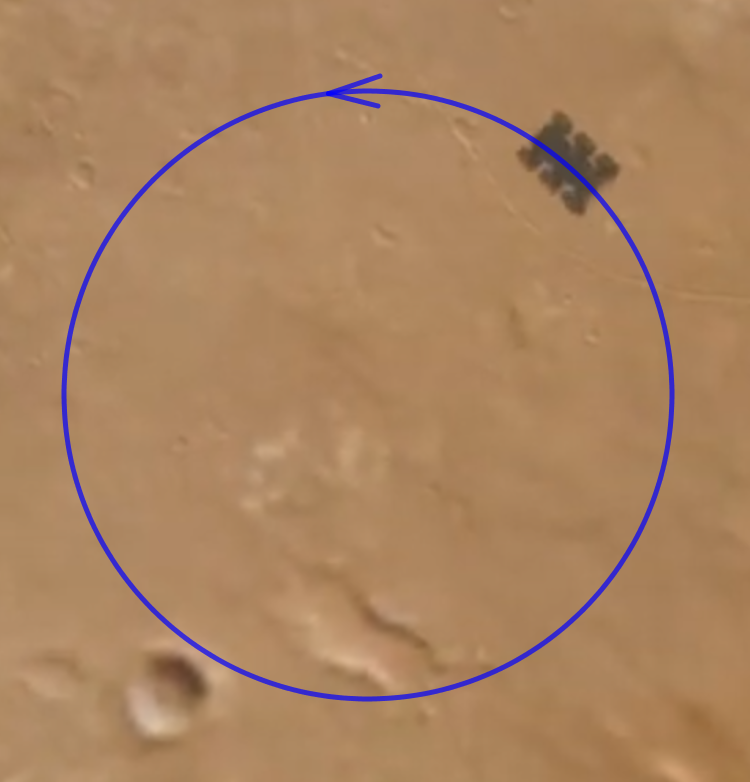
\includegraphics[width=.4\textwidth]{imagenes/img09-03.png}
	\end{figure}
\end{multicols}
\end{example}

\vspace{1cm}
\begin{center}
\begin{tikzpicture}
	\fill [left color=red!50, right color=teal!50] (0,0) rectangle (3.5,.02);
	\fill [left color=teal!50, right color=blue!50] (3.5,0) rectangle (7.5,.02);
	\end{tikzpicture}
\end{center}
\vspace{1cm}

\begin{myexampleblock}{Ligaduras}

\vspace{2mm} Las restricciones al movimiento en sistemas mecánicos reciben el nombre de \emph{ligaduras o vínculos}. Hay varias formas de clasificar las ligaduras. En Mecánica Teórica, la distinción más importante es entre ligaduras holónomas y no holónomas.

\vspace{2mm}  \textbf{Tipos de ligaduras}:

\vspace{2mm} Los dos criterios principales son si las ligaduras son integrables (permiten reducir el número de grados de libertad) o no y si contienen explícitamente al tiempo o no. Una ligadura no lineal se representa generalmente como una relación entre las coordenadas generalizadas necesarias para describir un sistema así como sus derivadas. Así una ligadura es cualquier expresión del tipo: $\ \Phi(q_i,\dot q_i, \ddot q_i,\cdots ,t)=0$

\begin{adjustwidth}{20pt}{5pt}
\vspace{2mm} $\triangleright \ $ Respecto a la integrabilidad de las ligaduras los sistemas se clasifican en:

\begin{adjustwidth}{20pt}{5pt}
\vspace{2mm} --- \emph{Ligaduras holónomas}. Si la expresión anterior es constante respecto a las derivadas la coordenada se llama holónoma. En ese caso las ligaduras pueden escribirse de la forma $f_j(\vec r_1, \vec r_2, \cdots \vec r_i, t)=0$. Nótese que el número $\ j \ $  condiciona al número de coordenadas que pueden existir, por lo que suele decirse que éstas ligaduras permiten eliminar grados de libertad al sistema.

\vspace{2mm} --- Ligaduras no holónomas. Cuando las coordenadas no pueden escribirse como holónomas. Así las ligaduras no holónomas no permiten eliminar los grados de libertad de un sistema. Estas ligaduras pueden clasificarse adicionalmente en lineales y no lineales.
\end{adjustwidth}

\vspace{2mm} $\triangleright \ $ Respecto a si las expresiones matemáticas que contienen las ligaduras contienen o no la variable tiempo las ligaduras se clasifican en:

\begin{adjustwidth}{20pt}{5pt}
\vspace{2mm} --- Ligaduras esclerónomas cuando las ligaduras son independientes del tiempo.

\vspace{2mm} --- Ligaduras reónomas cuando contienen al tiempo explícitamente, o sea son dependientes del tiempo.
\end{adjustwidth}
\end{adjustwidth}


\vspace{2mm} Algunos ejemplos de ligaduras son:

\begin{adjustwidth}{20pt}{5pt}
\vspace{2mm} --- Partícula moviéndose sobre una curva plana conocida $y = f(x)$, esta ligadura es holónoma.

\vspace{2mm} --- Rodamiento sin deslizamiento (ligadura lineal no holónoma), una rueda orientable de radio $R$ apoya sobre un plano sin deslizar.
\end{adjustwidth}
\vspace{2mm} 
	
\end{myexampleblock}

\chapter{Ejemplo de ligaduras no holónomas}

	\begin{tikzpicture}
	\fill [left color=red!50, right color=teal!50] (0,0) rectangle (6.5,.1);
	\fill [left color=teal!50, right color=blue!50] (6.5,0) rectangle (11.5,.1);
	\end{tikzpicture}



\vspace{10mm}
\begin{adjustwidth}{50pt}{50pt}
\begin{ejemplo}
Ejemplo de ligaduras no holónomas: cuerpo sin fricción sobre plano inclinado sin fricción.
\end{ejemplo}
\end{adjustwidth}
\vspace{5mm}

\section{Ejemplo de ligaduras no holónomas}

\begin{example}
	
\begin{multicols}{2}
\begin{figure}[H]
	\centering
	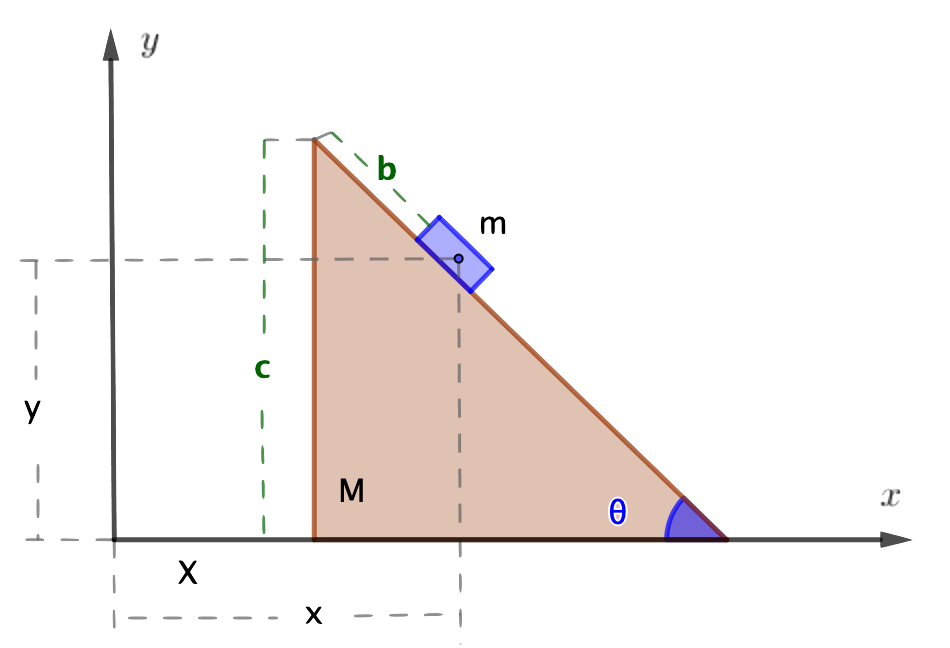
\includegraphics[width=.45\textwidth]{imagenes/img10-01.png}
\end{figure}	
$\,$

Una cuña de masa $M$ y pendiente $\theta$ se puede desplazar a lo largo del eje $x$. En su plano inclinado se encuentra otra masa $m$, que se puede desplazar por la pendiente. Ambas masas se desplazan \emph{sin rozamiento} ($M$ en el plano horizontal y $m$ en el plano inclinado de la cuña).
\end{multicols}
\end{example}

\normalsize{Supongamos}, en un principio, que ambas masas evolucionan libremente. Más tarde impondremos la restricción de que $m$ lo haga sobre el plano inclinado de $M$ (ligadura).

El lagrangiano del sistema será:

\begin{equation}
L \ = \ \ \ \dfrac M 2 \dot X^2 \ \ \ + \ \ \  \dfrac m 2 (\dot x^2 + \dot y^2) \ - \  mgy  \qquad \qquad \textcolor{gris}{(q_1=X;\ q_2=x; \ q_3=y)}
\end{equation}

Escribamos las ecuaciones de Euler-Lagrange correspondientes a este lagranginao, más tarde las completaremos al imponer las ligaduras del problema.
\begin{equation}
\label{T10EELsinL}
\displaystyle
\begin{cases} 
\ \displaystyle \dv{t} \left(\pdv{L}{\dot X}\right) - \pdv{L}{X} = \framebox{\textcolor{white}{lig}} \\ 
\ \displaystyle \dv{t} \left(\pdv{L}{\dot x}\right) - \pdv{L}{x} \ = \framebox{\textcolor{white}{lig}} \\ 
\ \displaystyle \dv{t} \left(\pdv{L}{\dot y}\right) - \pdv{L}{y} \ = \framebox{\textcolor{white}{lig}}
\end{cases}
\to \
\begin{cases}
\ \displaystyle \dv{t}(M\dot X)-0 \ =	\framebox{\textcolor{white}{lig}} \\
\ \displaystyle \dv{t}(M\dot x)-0 \ \ \ =	\framebox{\textcolor{white}{lig}} \\
\ \displaystyle \dv{t}(M\dot y)+mg=	\framebox{\textcolor{white}{lig}} 
\end{cases}
\to \
\begin{cases}
\ M \ddot X &= \framebox{\textcolor{white}{lig}} \\
\ m \ddot x	 &= \framebox{\textcolor{white}{lig}} \\
\ m\ddot y + mg &= \framebox{\textcolor{white}{lig}}
\end{cases}
\end{equation}

En las zona $\ \framebox{\textcolor{white}{lig}} \ $ es donde aparecerán los \emph{multiplicadores de Lagrange} correspondientes a las ligaduras del problema.

Para introducir las ligaduras del problema vamos a crear dos variables auxiliares momentáneas $\textcolor{teal}{c}$ y $\textcolor{teal}{b}$ (ver figura del ejemplo) que nos facilitarán el trabajo. ($\textcolor{teal}{c}$ es la altura de cuña y $\textcolor{teal}{b}$ la distancia qua ha bajado en el plano inclinado la masa $m$).


$\begin{cases}
\ x=X+b\cos \theta \\ \ y=c-b\sin \theta	
\end{cases} \to \textcolor{gris}{(2^a \ ec)} \ \ \ b=\dfrac {y-c}{-\sin \theta} \ \to \ \textcolor{gris}{(1^a \ ec)} \ \ \ x=X-\dfrac{y-c}{\sin \theta} \cos \theta$

Derivando esta última expresión, $\quad \dot x = \dot X -\dfrac{\cos \theta}{\sin \theta} \ \dot y \qquad \textcolor{gris}{(c=cte;\ \dot c=0)}$

Multiplicando por $\sin \theta$ y ordenando esta expresión,

\begin{equation}
\label{T10ligadura}
\subrayado{\boxed{ \ \boldsymbol{ \sin \theta \ \dot X \ - \ \sin \theta \ \dot x \ - \ \cos \theta \ \dot y \ = \ 0 } \ }	}
\end{equation}

que es nuestra relación de \textbf{ligadura no holónoma}. Identificando con
la definición: $\ a_{11}q_1+a_{12}q_2+a_{13}q_3=a_{10}$, determinamos que, en nuestro caso,

\begin{equation}
\boldsymbol{ a_{11} = \sin \theta;\ \ a_{12}=-\sin \theta;\ \ a_{13}=-\cos \theta;\ \ a_{10}=0 }
\end{equation}
Y ahora volveremos con las ecuaciones de Euler-Lagrange.

\vspace{10mm}
\underline{Inciso}: $\quad$ \rule{150pt}{0.1pt} $\quad$ Teoría.
\vspace{3mm}
\begin{ejemplo}
\begin{myblock}{Ecuaciones de Euler-Lagrange para el caso de ligaduras no holónomas.}
\vspace{3mm}
\begin{large}
\begin{equation}
\boldsymbol{
\dv{t} \left( \pdv{L}{\dot q_j}\right) - \pdv{L}{q_j} \ = \ \sum_{k=1}^p \lambda_k \ a_{kj}
}
\end{equation}
\end{large}
%\vspace{2mm} 
\begin{center}\textcolor{gris}{$p$ es el número de ligaduras y $j$ el de coordenadas generalizadas}\end{center}	
\end{myblock}
\end{ejemplo}
\vspace{-5mm}
\begin{flushright}
\rule{300pt}{0.1pt}	
\end{flushright} 
\vspace{5mm}

En nuestro caso solo tenemos una ligadura (ec. \ref{T10ligadura}):

\begin{equation}
\label{T10multiplicadores}	
\quad \displaystyle 
\boxed{ \ \boldsymbol{
\dv{t} \left( \pdv{L}{\dot q_j}\right) - \pdv{L}{q_j} \ = \  \lambda \ a_j
} \ }
\end{equation}

Retomamos nuestras ecuaciones de Euler-Lagrange, ec. \ref{T10EELsinL}, y vamos a imponer nuestras ligadura (ec. \ref{T10ligadura})  con los multiplicadores de Lagrange (ec \ref{T10multiplicadores}).


\begin{equation}
\label{T10EL}
\begin{cases}
\ M \ddot X &= \textcolor{gris}{\lambda a_{11}=}\ \ \ \lambda \sin \theta \\
\ m \ddot x	&= \textcolor{gris}{\lambda a_{12}=}-\lambda \sin \theta \\
\ m \ddot y - mg &= \textcolor{gris}{\lambda a_{13}=} - \lambda \cos \theta
\end{cases}	\qquad  \qquad 
\text{Ligadura:} \ \ \sin \theta \ \dot X \ - \ \sin \theta \ \dot x \ - \ \cos \theta \ \dot y \ = \ 0 \qquad
\end{equation}

Integrando,
$\quad \begin{cases}
\ M \dot X = (\lambda \sin \theta) \ t	+ A \\
\ m \dot x = -(\lambda \sin \theta) \ t + B \\
\ m \ddot y = (-\lambda \cos \theta - mg)\ t + C
\end{cases}
\ \to \quad
\begin{cases}
\ \dot X = \dfrac{\lambda \sin \theta}{M} \ t + \dfrac AM\\
\ \dot x = -  \dfrac{\lambda \sin \theta}{m} \ t + \dfrac Bm \\
\ \dot y = -  \dfrac{\lambda \cos \theta -mg}{m} \ t +\dfrac Cm
\end{cases}$

Incorporando estos tres resultados a la relación de ligadura (ec \ref{T10ligadura}),

$\sin \theta \left[ \dfrac{\lambda \sin \theta}{M} \ t + \dfrac AM \right] \sin \theta \left[  - 
 \dfrac{\lambda \sin \theta}{m} \ t + \dfrac Bm  \right] -  
 \cos \theta \left[ -  \dfrac{\lambda \cos \theta -mg}{m} \ t +\dfrac Cm \right] = 0$
 
 $\left[ 
\lambda  \dfrac{\sin^2 \theta}{M} + \lambda  \dfrac{\sin^2 \theta}{m} + \dfrac{\lambda \cos^2 \theta + mg \cos \theta}{m}
 \right]\ t +
 \left[
 \dfrac{A \sin \theta}{M} - \dfrac{B \sin \theta}{m} - \dfrac{C \cos \theta}{m} 
 \right]=0 \ , \qquad \forall t$ 

Necesariamente, mientras dure el movimiento (m sobre M, luego ya no es válida la ligadura impuesta), $Mt+N=0 \to M=N=0$, las constantes de la relación anterior han de ser ambas nulas (de lo contrario t=0 y la relación es válida para todo t mientras dure el movimiento).

Obtenemos las siguientes relaciones entre las constantes de integración:

\begin{multicols}{2}
\begin{equation}
	\quad\lambda  \left[ \left( \dfrac 1M + \dfrac 1m \right) \sin^2 \theta + \dfrac{\cos^2 \theta}{m} \right] = - g \cos \theta
\end{equation}

\begin{equation}
	\label{T10relacctesinteg}
	\dfrac{A \sin \theta}{M} - \dfrac{B \sin \theta}{m} - \dfrac{C \cos \theta}{m}=0 
\end{equation}
\end{multicols}

Trabajando con la primera de estas ecuaciones,

$\lambda \left[ \dfrac 1M \sin^2 \theta + \dfrac 1 m \cancelto{1}{(\sin^2 \theta + \cos^2 \theta)} \right] = - g \cos \theta \quad \to \quad \lambda= \dfrac{-g \cos \theta}{\dfrac 1 m + \dfrac {\sin^2 \theta} M }$

En función de cosenos, $\quad \lambda \ = \ \dfrac{-g \cos \theta}{\dfrac 1 m +\dfrac 1 M - \dfrac{\cos^2 \theta}{M} } \ = \ \dfrac{-mMg\cos \theta}{M+m-m\cos^2 \theta}$

Dividiendo numerador y denominador por $\ m+M\, , \qquad \lambda \ = \ \dfrac{-\dfrac{mM}{m+M}g \cos \theta}{1-\dfrac{m}{m+M}\cos^2 \theta}$

\begin{equation}
\label{T10lambda}
\boldsymbol{
\lambda \ = \ \dfrac{-\mu M g \cos \theta}{1-\mu \cos^2 \theta}} \, , \qquad \text{ con } \quad \mu \ = \ \dfrac{m}{m+M}	
\end{equation}

Llevando este resultado a la segunda de las ecuaciones E-L (ec \ref{T10EL}),

$\cancel{m} \ddot x = -\sin \theta \ \dfrac{- \dfrac{\cancel{m}M}{m+M} g \cos \theta}{1-\mu \cos^2 \theta} \quad \to \quad \ddot x =  \dfrac{\dfrac{M}{m+M} g \sin \theta \cos \theta}{1-\mu \cos^2 \theta}$

Como $\quad \mu-1=\dfrac{m}{m+M} -1 = \dfrac{-M}{m+M} \quad \to \quad \dfrac{M}{m+M}=\mu-1\, , \ $ por lo que

\begin{equation}
\label{T10lambda2}
\boxed{ \ \boldsymbol{
\lambda \ = \ \dfrac{-m(1-\mu) g \cos \theta}{1-\mu \cos^2 \theta}} \ } \ , \qquad \text{ con } \quad \mu \ = \ \dfrac{m}{m+M}	
\end{equation}

\begin{equation}
\label{T10ecx} 
\boxed{ \ \boldsymbol{ \ddot x \ = \ \dfrac{(1-\mu) \ g \ \sin \theta \ \cos \theta}{1 \ - \ \mu \cos^2 \theta} } \ }	
\end{equation}

Acudiendo a la tercera de las ecuaciones E-L (ec \ref{T10EL}),
$\quad \ddot y = \dfrac{-\lambda \cos \theta}{m}-g=\dfrac{\cancel{m} (1-\mu) g \cos \theta}{1-\mu \cos^2 \theta}-g$

\begin{equation}
\label{T10ecx} 
\boxed{ \ \boldsymbol{ \ddot y \ = \ \dfrac{(1-\mu) \ g  \ \cos^2 \theta}{1 \ - \ \mu \cos^2 \theta} - g  } \ }	
\end{equation}

Yendo a la primera de las ecuaciones E-L (ec \ref{T10EL}), $\quad \ddot X=\dfrac{\sin \theta}{M} \lambda=\dfrac{\sin \theta}{M}  \dfrac{-m(1-\mu) g \cos \theta}{1-\mu \cos^2 \theta}$

\begin{equation}
\label{T10ecx} 
\boxed{ \ \boldsymbol{ \ddot X \ = \ - \dfrac m M \ \dfrac{(1-\mu) \ g \ \sin \theta \ \cos \theta}{1 \ - \ \mu \cos^2 \theta} } \ }	
\end{equation}

Estas tres últimas ecuaciones enmarcadas $  \  ( \ddot X,\ \ddot x,\ \ddot y  ) \ $, junto con la relación de las contantes de integración anteriormente establecidas (ec \ref{T10relacctesinteg}) proporcionarán, una vez integradas, las ecuaciones de movimiento.


Resumiendo,

\begin{adjustwidth}{100pt}{10pt}
	
$\boldsymbol{ \ddot x \ = \ \dfrac{(1-\mu) \ g \ \sin \theta \ \cos \theta}{1 \ - \ \mu \cos^2 \theta} }$

$\boldsymbol{ \ddot y \ = \ \dfrac{(1-\mu) \ g  \ \cos^2 \theta}{1 \ - \ \mu \cos^2 \theta} - g }$


$\boldsymbol{ \ddot X \ = \ - \dfrac m M \ \dfrac{(1-\mu) \ g \ \sin \theta \ \cos \theta}{1 \ - \ \mu \cos^2 \theta} }$


$\boldsymbol{ \dfrac{A \sin \theta}{M} - \dfrac{B \sin \theta}{m} - \dfrac{C \cos \theta}{m}=0 }$

\end{adjustwidth}

\subsection{Análisis de casos límites}
\begin{tikzpicture}
	\fill [left color=red!50, right color=teal!50] (0,0) rectangle (3.5,.01);
	\fill [left color=teal!50, right color=blue!50] (3.5,0) rectangle (7.5,.01);
	\end{tikzpicture}
\vspace{0.5cm}

$\boldsymbol \triangleright \ $ \textbf{Caso límite:} $\boldsymbol{\quad M\to \infty \ \Rightarrow \ \mu \to 0} \ \longrightarrow \ \begin{cases}
 \ \ddot X &=0 \\ \ \ddot x &= g \cos \theta \\ \ \ddot y &=g \cos^2 \theta - g =-g\sin^2 \theta	
 \end{cases}$ 
 
 Que coincide con los resultados que hubiésemos obtenido con mecánica newtoniana, como veremos al final del tema.
 
  \vspace{5mm}
  
\begin{myexampleblock}{Caso $M\to \infty$ con mecánica newtoniana}
 	
 	\begin{multicols}{2}
\begin{figure}[H]
	\centering
	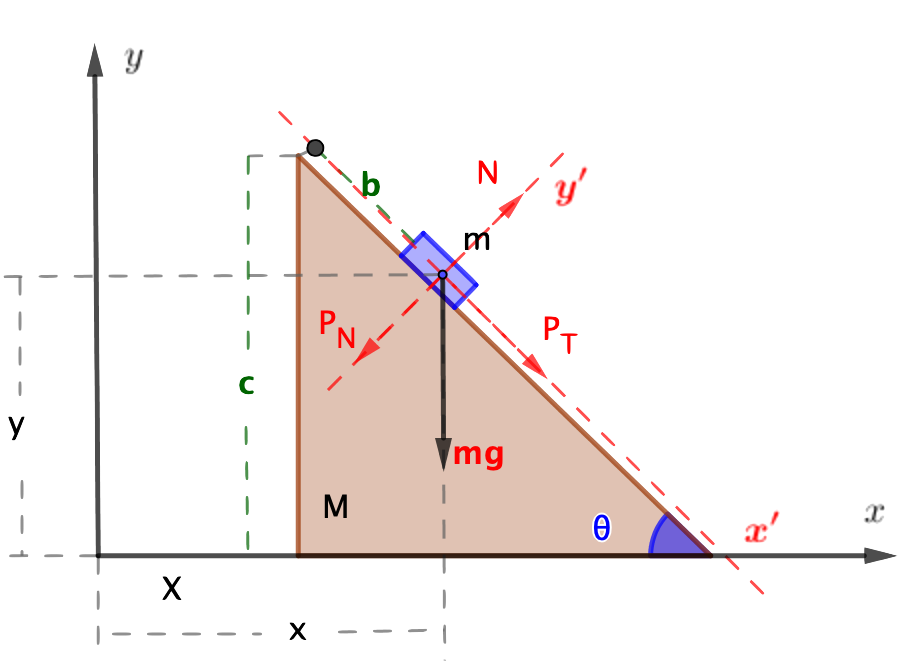
\includegraphics[width=.45\textwidth]{imagenes/img10-02.png}
\end{figure}	
$\,$

$m$ se desplaza por el plano inclinado.

La componente $P_N$ se anula con la reacción $N$ del plano, solo queda la componentes $P_T=mg\sin \theta$. Solo hay movimieto en el eje $x'$.

Segunda de Newton: $º F_mg\sin \theta = ma$

Luego $a=g\sin \theta$

La proyección del vector $\vec a$ del eje $x`$ sobre los ejex $x$ e $y$ dan unas aceleraciones:
\end{multicols}
$a_x=\ddot x= g\sin \theta \cos \theta;\quad a_y=\ddot y= -g\sin^2 \theta\, , \ $ que coinciden con las que homos obtenido más arriba.
 \end{myexampleblock}
 
\vspace{1cm}
  

$\boldsymbol \triangleright \ $ \textbf{Caso límite:} $\quad \boldsymbol{\theta = 0}\, , \ $ la masa $m$ reposa sobre $M$.

Se obtiene, $\quad \ddot X=0;\quad \ddot x=0;\quad \ddot y=\dfrac{(1-\mu)g}{1-\mu}=g$, pero $\ \ddot y=0 \ $ al estar $m$ en el suelo.

\rule{200pt}{0.1pt}

Se cumplen perfectamente los casos límites.


 
 



\chapter{Transformación de \emph{Legendre}}

	\begin{tikzpicture}
	\fill [left color=red!50, right color=teal!50] (0,0) rectangle (6.5,.1);
	\fill [left color=teal!50, right color=blue!50] (6.5,0) rectangle (11.5,.1);
	\end{tikzpicture}
	
\vspace{10mm}
\begin{adjustwidth}{50pt}{50pt}
\begin{ejemplo}
La transformada de Legendre es una pieza clave para estudiar el \emph{formalismo hamiltoniano}. Es un mecanismo matemático que se usa, además de en mecánica teórica, en termodinámica.
\end{ejemplo}
\end{adjustwidth}
\vspace{5mm}

\section{La tranformada de \emph{Legendre}}

Una función $f(x)$ almacena información. \emph{Legendre} se preguntó si podía inventarse algún procedimiento que pase a una nueva función $g$, con una nueva variable $p$, tal que la información que estaba en la función original $f$ también esté en la nueva función $g$ y, aún más, si volvemos a efectuar el procedimiento recuperemos la función $f$ original.

Esquemáticamente, llamando $\ \boldsymbol {\hat{A}} $ a la operación a efectuar (procedimiento o transformada de Legendre), 

$$\subrayado{ \boxed{ \ \boldsymbol{ f(x) \qquad \underrightarrow{\quad \hat{A} \quad} \qquad g(p) \qquad  
\underrightarrow{\quad \hat{A} \quad} \qquad f(x) } \ }}$$

Dada $\ f(x)\ \, , \ $ construimos $\quad \hat A \ f(x) \ = \ f'(x)\cdot x \ - \ f(x) \ = \ \left[ x\ \displaystyle \dv{x} -1 \right] \ f(x)$

En general, la variable no tiene por que se $x$, llamémosla $\ \ \textcolor{red}{var.\ origen} \, , \ $ así,

\begin{equation}
 \ \boldsymbol{
\hat A \ = \ \displaystyle \left[ \textcolor{red}{var.\ origen}\ \dv{\ \textcolor{red}{var.\ origen}} - 1 \right]
} 	
\end{equation}

Elegimos que la nueva variable sea:

\begin{equation}
\ \boldsymbol{
 \displaystyle \textcolor{blue}{nueva \ vble.} \ = \ \dv{f}{\ \textcolor{red}{var.\ origen}}
} 		
\end{equation}

Resumiendo, la forma de definir una \textbf{transformada de Legendre} es:

\begin{multicols}{2}
$\boxed{ \ \boldsymbol{
\hat A \ = \ \displaystyle \left[ \textcolor{red}{var.\ origen}\ \dv{\ \textcolor{red}{var.\ origen}} - 1 \right]
} \ }$

$\boxed{ \ \boldsymbol{
 \displaystyle \textcolor{blue}{nueva \ vble.} \ = \ \dv{f}{\ \textcolor{red}{var.\ origen}}
} \ }$	
\end{multicols}

Veamos un ejemplo.

\subsection{Ejemplo de transformada de \emph{Legendre}}
\begin{tikzpicture}
	\fill [left color=red!50, right color=teal!50] (0,0) rectangle (3.5,.01);
	\fill [left color=teal!50, right color=blue!50] (3.5,0) rectangle (7.5,.01);
	\end{tikzpicture}
\vspace{0.5cm}

\begin{example}

.	\vspace{2mm} \textbf{Ejemplo de transformada de Legendre	}

\vspace{2mm} $\boxed{ \ \boldsymbol{f(x) \ = x^2} \ }$

\vspace{2mm} Nueva variable: $\quad p=\displaystyle \dv{f}{x} = f'(x)=2x \ \to \ \boxed{\ x=\dfrac p 2 \ }$

\vspace{2mm} $\displaystyle g(p)=\hat A f(x)=\left[x\dv{x}-1\right] f(x) = \left[x\dv{x}-1\right] \ (x^2) = x(2x)-x^2=2x^2-x^2=x^2=\left( \dfrac p 2 \right)^2= \dfrac{p^2}{4}$

\vspace{2mm} $\boxed{ \boldsymbol{ \ g(p)\ = \dfrac{p^2}{4} } \ }$

\vspace{2mm} Volvamos a plicar $\hat A$ a $g$ para ver si recuperamos la $f$ original.

\vspace{2mm} Nueva variable: $\quad t=\displaystyle \dv{p} g(p) = \dv{p} \left( \dfrac{p^2}{4} \right) =\dfrac p 2 \ \to \ \boxed{\ \boldsymbol{p=2t} \ }$

\vspace{2mm} $h(t)=\hat A g(p) = \displaystyle \left[p\dv{p}-1\right] \ g(p)=\left[p\dv{p}-1\right] \ \dfrac{p^2}{4} = p \dfrac{2p}{4}-\dfrac{p^2}{4}=\dfrac{p^2}{4}=\dfrac{(2t)^2}{4}=t^2$

\vspace{2mm} Por lo que $\quad \boxed{\ \boldsymbol{ h(t)=t^2 \ \leftrightarrow \ h \equiv f } \ }$

$$f(x) \qquad \underrightarrow{\quad \hat{A} \quad} \qquad g(p) \qquad  
\underrightarrow{\quad \hat{A} \quad} \qquad h(t) \equiv f(x)$$

\vspace{2mm} 
\end{example}

\begin{theorem}

 $$f\qquad \underrightarrow{\quad \hat{A} \quad} \qquad g \qquad  
\underrightarrow{\quad \hat{A} \quad}  \qquad f	$$

\vspace{0.1mm}
\end{theorem}
\textcolor{brown}{\rule{200pt}{0.3pt}}

\begin{proof}.
	
\vspace{2mm}	$f(x) \, ; \ \ p=\displaystyle \dv{f}{x} \ \to 	\quad \boldsymbol{g(p)}=\hat A f(x)= \left[x\dv{x}-1\right] f(x)=x\dv{f}{x}-x=\boldsymbol{xp-f}$

\vspace{2mm} $\displaystyle h(q)=\hat A g(p)= \left[p\dv{p}-1\right] g(p) = p\dv{g}{p}-g $

\vspace{2mm} $ \displaystyle \boxed{ \ \displaystyle{h} \ }= \left[p\dv{p}-1\right] g(p)=p\dv{p} \boldsymbol{(xp-f)}- \boldsymbol{(xp-f)}=p\left( \dv{x}{p} p + \bcancel{x \cancelto{1}{\dv{p}{p}}} - \dv{f}{p} \right) - \bcancel{xp} + f=$

$\displaystyle = p \left( \dv{x}{p} p  -\dv{f}{p} \right) + f=\textcolor{gris}{(p=\dv{f}{x})}  =p \left( \dv{x}{p} \cdot \dv{f}{x} - \dv{f}{p} \right) + f = p \left(\dv{f}{p}-\dv{f}{p} \right)+f=p (0) + f =\boxed{ \ \displaystyle{f} \ }$

\end{proof}

\subsection{Una interpretación de la transformada de \emph{Legendre}}
\begin{tikzpicture}
	\fill [left color=red!50, right color=teal!50] (0,0) rectangle (3.5,.01);
	\fill [left color=teal!50, right color=blue!50] (3.5,0) rectangle (7.5,.01);
	\end{tikzpicture}
\vspace{0.5cm}

El razonamiento de Legendre podría haber sido el siguiente:

\begin{multicols}{2}
\begin{figure}[H]
	\centering
	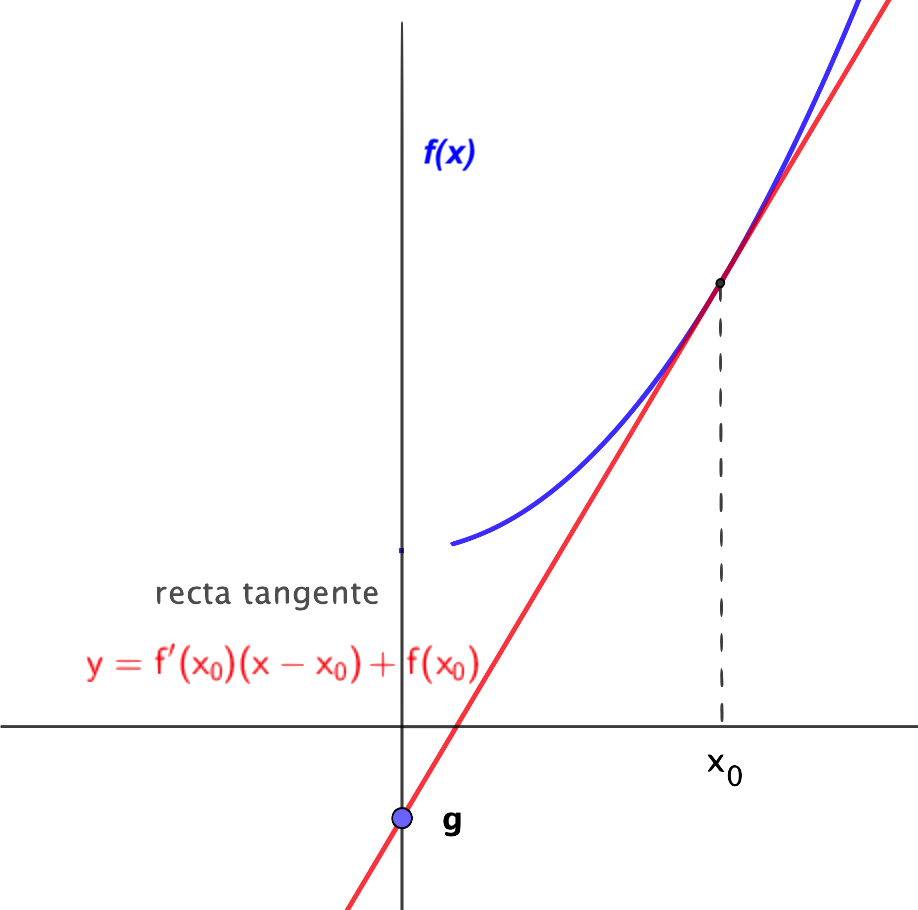
\includegraphics[width=.4\textwidth]{imagenes/img11-01.png}
\end{figure}
$\quad$

Dada una función $f(x)$ y un punto de su dominio $x_0$, llamamos $g$ al punto de corte de la recta tangente a $f(x)$ en $x_0$, $\ y=f'(x_0)(x-x_0)+f(x_0)\, ,$ con el eje de ordenadas ($y$):

$g=-x_of'(x_0)`f(x_0)$. $\quad$ Llamo $p=f'(x_0)\, , $ así:

$g \ = \ -x_0 \, p \ + \ f(x_0) \quad p$ es la pendiente de esta recta.
\end{multicols}

\begin{multicols}{2}
Para otro punto $g$ existirá otra recta tangente a $f$. Teniendo en cuenta todas las posibles pendientes de las rectas tangentes a f(x) tenemos la \emph{transformada de Legendre}. Se trata de encontrar en qué posición del eje $y$ me debo encontrar para lanzar un proyectil desde allí y que sea tangente a $f(x)$. Conocidas todas estad $g$, conoceríamos la \emph{``envolvente''} de la función original y conservaríamos la información que ella guarda.

\begin{figure}[H]
	\centering
	\includegraphics[width=.4\textwidth]{imagenes/img11-02.png}
\end{figure}
\end{multicols}


\begin{multicols}{2}
\begin{figure}[H]
	\centering
	\includegraphics[width=.4\textwidth]{imagenes/img11-03.png}
\end{figure}	
Hemos visto que $\ g=-x_0p+f_0 = \left[ \displaystyle -x\dv{x} +1 \right]\ f$

En termodinámica se define de modo opuesto (un cambio de signo) debido a cuestiones históricas.

Lo podemos reinterpretar como que hay que disparar desde $y>0$ hacia el ej $X$ para que, al rebotar el proyectil en el eje, salga tangente (\emph{rasante}) hacia la función $f(x)$.

\begin{small}\textcolor{gris}{(Transformada de Legendre o los ``disparos rasantes'').}\end{small}

\end{multicols}

\section{Como prodría haber razonado \emph{Hamilton}}
Hamilton conoce el trabajo de Lagrange. Recibe el trabajo de Legendre sobre su transformada y se pregunta qué ocurriría si aplica la transformada al lagrangiano $L$. Obtendré una nueva función que llamaré \emph{hamiltoniano}, $H$, que contendrá la información del lagrangiano: $\subrayado{ \quad \boxed{\ L \qquad \underrightarrow{\quad \hat{A} \quad} \qquad H \ } }$ 


Mecánica clásica 1D (1 dimensión): $\quad L=\dfrac m 2 \dot x^2 - V(x)$

$L(x,\dot x)$, la transformada de Legrendre depende de una sola variable. La variable que nos interesa es $v=\dot x$ que es a la que vamos a aplicar la transformada. Como hay más de una variable, en vez de usar \emph{derivadas totales} usaremos \emph{derivadas parciales}.

$H(p)=\dot A \ L(v)= \left[ v \displaystyle \pdv{v} -1 \right] \ L =\left[ v \displaystyle \pdv{v} -1 \right] \left( \dfrac m 2 v^2 - V(x) \right)$

La nueva variable es $\quad p=\displaystyle \pdv{v} L =mv \ \to \ v=\dfrac p m$

$H(p)=\displaystyle v\pdv{v} (mv^2-V(x)) - (mv^2-V(x))=
v(mv-0)-\dfrac m2 v^2 + V(x)= \dfrac m 2 v^2 + V(x)$

Con la nueva variable,

$H(p)=\displaystyle \dfrac m 2 \left( \dfrac p m \right)^2 + V(x)$

\begin{equation}
H(p) \ = \ \dfrac{p^2}{2m} \ + \ V(x)	
\end{equation}

?`Es $\ H(x,p)\ $ constante en el tiempo?

$\displaystyle \dv{H}{t}=  \dv{H}{p} \dv{p}{t} + \dv{V}{x} \dv{x}{t}=
\dfrac{2p}{2m} \dot p + \dv{V}{x} \dv{x}{t}=\dfrac{p}{m} \dot p + \dv{V}{x} \dot x \qquad $
Como $\quad \dot x=v=\dfrac p m$,

$\displaystyle \dv{H}{t}   
= \dfrac{p}{m} \dot p + \dv{V}{x} \dfrac p m
= \dfrac p m \left[ \dot p + \dv{V}{x} \right]=\dfrac p m \left[ \dot p + V'(x) \right]$

Newton: $\quad	\displaystyle \dot p = - \dv{V}{x} = - V' (x) \ \to \ \dot p +  V' (x)=0$

Por lo que $\quad \displaystyle \dv{H}{t} \ = \ 0 \quad \to \quad H(x,p)=cte \ del \ movimiento$, con dimensiones de \emph{energía}.

Con el Hamiltoniano tenemos otra formulación alternativa a la lagrangiana y, además, aún más potente que ella.




\chapter{Hamiltoniano vs Energía}

	\begin{tikzpicture}
	\fill [left color=red!50, right color=teal!50] (0,0) rectangle (6.5,.1);
	\fill [left color=teal!50, right color=blue!50] (6.5,0) rectangle (11.5,.1);
	\end{tikzpicture}

\vspace{1cm}

\begin{adjustwidth}{50pt}{50pt}
\begin{ejemplo}
	Hay una relación entre el hamiltoniano $H$ y la energía $E$. Al principio suele haber confusión entre qué es una cosa y otra, en este capítulo se intentará aclarar estos conceptos antes de entrar de lleno en el formalismo hamiltoniano.
\end{ejemplo}
\end{adjustwidth}
	
\vspace{1cm}

\section{Recordatorios}

\begin{large}
\begin{myalertblock}
\text{Transformada de Legendre}
$$\quad g(\textcolor{red}{\blacktriangle}) \ = \ \widehat A  \ f (\textcolor{blue}{\blacksquare)} \ = \ \left[ \textcolor{blue}{\blacksquare} \ \pdv{\ \textcolor{blue}{\blacksquare}} - 1 \right] \ f (\textcolor{blue}{\blacksquare)} \, ; \qquad \textcolor{red}{\blacktriangle} \ = \ \pdv{f}{\ \textcolor{blue}{\blacksquare}}	$$
\end{myalertblock}
\end{large}
\vspace{5mm}

\begin{definition}

\textbf{Función homogénea de grado cero}: $\qquad \qquad \boldsymbol {\boxed{ \ f(\lambda x) \ = \ \lambda^n\ f(x) \ } }$	
\end{definition}

\underline{Ejemplo}: $\quad f(x)=x^2 \ $ es función homogénea de grado 2:

$f(x)=x^2 \to \ f(\lambda x)=(\lambda x)^2=\lambda^2 x^2 = \lambda^{\boldsymbol{2}} f(x)$

\underline{Extensión a varias variables}: $\quad f(x,y,z)=x^2+y^2+3xz\ $  es función homogénea de grado 2:

$f(\lambda x,\lambda y, \lambda z)=(\lambda x)^2+(\lambda y)^2 +3(\lambda x)(\lambda y)=\lambda^2 (x^2+y^2+3xy)=\lambda^{\boldsymbol{2}} f(x)$

\underline{Otro ejemplo}: $\quad f(x,y)=\dfrac{xy}{x^2+y^2}\ $ es función homogénea de grado 0:

$f(\lambda x,\lambda y)=\dfrac{\lambda x \ \lambda y}{(\lambda x)^2+(\lambda y)^2}= \dfrac{\cancel{\lambda ^2} \ xy}{\cancel{\lambda^2} (x^2+y^2)}=\dfrac{xy}{x^2+y^2}=\lambda^{\boldsymbol{0}} f(x)$

\vspace{5mm}
\textbf{?`Cuál es la aplicación de las funciones homogéneas?}

\begin{theorem}

\textbf{Teorema de Euler}

\begin{equation}
\label{T12ThEuler}
\boldsymbol{
f(x_1,\cdots ,x_p) \text{ homogénea grado } n \ \ \longrightarrow \ \ 
x_1\dv{f}{x_1} + \cdots + x_p\pdv{f}{x_p} \ = \ n \ f
}	
\end{equation}	
\end{theorem}

\begin{proof} (en una dimensión)

$f(\lambda x)=\lambda^n f(x)\, ; \qquad y=\lambda x \ \to f(y)=\lambda ^n f(x)\ $. Derivando ambas expresiones respecto de lambda,

\hspace{2cm} $\displaystyle \pdv{\lambda} [f(y)] = \pdv{\lambda} [\lambda^n f(x) ] $

\hspace{2cm} $\displaystyle \pdv{f(y)}{y} \ \  \cancelto{x}{\pdv{y}{\lambda}} = n \lambda^{n-1} f(x)\, , \qquad \forall \lambda$

\hspace{2cm} $\displaystyle x \ \pdv{f(y)}{y} = n \lambda^{n-1} f(x) \, , \qquad \forall \lambda$

\hspace{2cm} Para $\lambda=1 \ \to \ \displaystyle x \ \pdv{f(y)}{y} = n \ f(x)$

\hspace{2cm} Cuando $\ y=1.x \ \to \ \ \displaystyle x \ \pdv{f(x)}{x} = n f(x)$
\end{proof}



\vspace{5mm}
\section{Energía cinética}
\label{T12Tesfericas}

$$\boldsymbol {T \ = \ \dfrac m 2 \ v^2 \ = \ \dfrac m 2 \ \vec v \cdot \vec v }$$


$\triangleright \ $ En coordenadas cartesianas:

$v^2=\vec v \cdot \vec v= \mqty(v_1&v_2&v_3) \mqty(v_1\\v_2\\v_3)=\mqty(v_1&v_2&v_3) \mqty(\imat{3}) \mqty(v_1\\v_2\\v_3)=
v_1^2+v_2^2+v_3^2$

\begin{scriptsize} \textcolor{gris}{$I=\mqty(\imat{3}) \ $ es la métrica en el espacio plano $\mathbb R^3$} \end{scriptsize}


$T$ en cartesianas, $\quad  \boxed{ \ T \ = \ \dfrac m 2 \ ( \ \dot x^2 + \dot y^2 + \dot z^2 \ ) \ }$

$\triangleright \ $ En coordenadas esféricas:

\begin{multicols}{2}
	\begin{figure}[H]
	\centering
	\includegraphics[width=.3\textwidth]{imagenes/img12-01.png}
\end{figure}
$\quad$

$\quad \begin{cases}
\ x \ = \ r\ \sin \theta \ \cos \phi \\
\ y \ = \ r\ \sin \theta \ \sin \phi \\
\ z \ = \ r\ \cos \theta  	
\end{cases}$

\end{multicols}

Para expresar la energía cinética en esféricas necesitamos:

$\begin{cases}
\ \dot x \ = \	\dot r \sin \theta \cos \phi \ + \ r \cos \theta \ \dot \theta \cos \phi \ - \  r \sin \theta \sin \phi \ \dot \phi \\
\ \dot y \ = \	\dot r \sin \theta \sin \phi \ + \ r \cos \theta \ \dot \theta \sin \phi \ + \  r \sin \theta \cos \phi \ \dot \phi \\
\ \dot z \ = \ \dot r \cos \theta \ - \ r \sin \theta \ \dot \theta
\end{cases} \ \to \ \ \dot x^2; \ \dot y^2;\ \dot y^2 \ \to \ \sum \ \ \cdots$

Tras largos cálculos (que se recomiendan hacer, al menos una vez), se obtiene

$$\boldsymbol{\dot x^2 + \dot y^2 + \dot z^2 \ = \ \dot r^2 \ + \ r^2 \ \dot \theta^2 \ + \ r^2 \ \sin^2 \theta \ \dot \phi^2}$$ 

\vspace{3mm}
\ul{Inciso-1} $\quad$ \rule{50pt}{0.1pt} $\quad$ \begin{small} \textbf{Usando geometría diferencial} \end{small} \begin{footnotesize} (Cap 11 ``Relatividad General'' de Javier García).\end{footnotesize} 

$g_{ij} \ = \ \mqty( 1&0&0 \\ 0&r^2&0 \\ 0&0&r^2 \sin^2 \theta) $

$\vec v \cdot \vec v= g_{ij}\ v^i \ v^j= 1 \ v^r v^r \ + \ r^2 \ v^\theta v^\theta \ + \ r^2 \sin^2 \theta \ v^\phi v^\phi \, ; \qquad v^r=\dot r;\ v^\theta=\dot \theta;\  v^\phi=\dot \phi$

$v^2 \ = \ \dot r^2 \ + \ r^2 \ \dot \theta^2 \ + \ r^2 \ \sin^2 \theta \ \dot \phi^2 \qquad $ llegamos, más rápidamente, al mismo resultado. 

\vspace{-5mm}
\begin{flushright} \rule{200pt}{0.1pt} \end{flushright}

$T$, en esféricas, es pues: $\quad \boxed{ \ T \ = \ \dfrac m 2 \ (\ \ \dot r^2 \ + \ r^2 \ \dot \theta^2 \ + \ r^2 \ \sin^2 \theta \ \dot \phi^2 \ ) \ } $


\vspace{5mm} \textbf{$T$ homogénea de grado}, tanto en cartesianas como en esféricas, por lo que podemos aplicar el \emph{teorema de Euler}:

$T(v_1,v_2,v_3) \ = \ \dfrac m 2 (v_1^2+v_2^2+v_3^2) \ \ \underrightarrow{\ \  \text{Th. Euler} \ \ }  \ \  
\displaystyle v_1\ \pdv{v_1}+v_2\ \pdv{v_2}+v_2\ \pdv{v_3} \ = \ 2\ T$

$T(v_r,v_\theta,v_\phi) \ = \ \dfrac m 2 (v_r^2+v_\theta^2+v_\phi^2) \ \ \underrightarrow{\ \  \text{Th. Euler} \ \ }  \ \  
\displaystyle v_r\ \pdv{v_r}+v_\theta\ \pdv{v_\theta}+v_\phi \ \pdv{v_\phi} = \ \dot r\ \pdv{v_r}+\dot \theta \ \pdv{v_\theta}+ \dot \phi \ \pdv{v_\phi}  = \ 2\ T$

\vspace{5mm} \textbf{--- No todas las $\boldsymbol T$ son funciones homogéneas de grado dos.}

\begin{multicols}{2}
	\begin{figure}[H]
	\centering
	\includegraphics[width=.3\textwidth]{imagenes/img12-02.png}
\end{figure}
$\quad$

El palo $r$ está obligado (motor externo) a oscilar. La masa $m$ se puede mover libremente por $r$, sin fricción. 

?`Cuál será el movimiento de $m$ sometida a esta restricción?

\end{multicols}

$T$ en esféricas, con $\theta=\dfrac {\pi}{2}$ y con $\dot \theta = 0$,

$T=\ \dfrac m 2 \ (\ \dot r^2  +  r^2 \ \cancelto{0}{\dot \theta^2}  +  r^2 \ \cancelto{1}{\sin^2 \theta }\ \dot \phi^2  ) \ = \ \dfrac m2 \ (\dot r^2 + r^2\ \dot \phi^2)$

Introducimos la ligadura $\ \phi=\sin t \ \to T=\dfrac m 2 (\dot r^2 + r^2 \cos^2 t)=T(\dot r)$, no homogénea:

$T(\lambda \dot r)=\dfrac m 2 \left( (\lambda^2 \dot  r)^2 + r^2 \cos^2 t \right) \neq \lambda^n T(r) \, , \ $ no homogénea.

$\vec r=(r\cos \phi, r \sin \phi)=r\left( \cos(\sin t),\ r\sin(\sin t) \right) \ \to \ $ T no homogénea por aparecer $t$ explícitamente en el cambio de coordenadas cartesianas a generalizadas y no se puede aplicar el teorema. de Euler.


\vspace{5mm}
Conclusión:
\vspace{3mm}
\begin{adjustwidth}{20pt}{0pt}
\begin{destacado}
\emph{Si al hacer el cambio de coordenadas cartesianas a generalizadas $\ (x,y,x \to q_i, q_2, \dots)\ $ si no aparece el tiempo $t$ de manera explícita, $T$ será homogénea de grado 2 y se podrá aplicar el teorema de Euler.}	
\end{destacado}
\end{adjustwidth}





\vspace{5mm}
\section{?`Es el lagrangiano constante en el tiempo?}


$L(q_j, \dot q_j, t) \ \to \ \displaystyle \dv{L}{t}=\sum_{j=1}^n  \pdv{L}{q_j} \ \pdv{q_j}{t} + \sum_{j=1}^n  \pdv{L}{\dot q_j} \ \pdv{\dot q_j}{t} + \pdv{L}{t} = \sum_{j=1}^n  \pdv{L}{q_j} \ \dot q_j + \sum_{j=1}^n  \pdv{L}{\dot q_j} \ \ddot q_j + \pdv{L}{t}$

Ecuaciones Euler-Lagrange: $\ \displaystyle \dv{t} \left( \pdv{L}{\dot q_j} \right) = \pdv{L}{q_j}$,

$\displaystyle \dv{L}{t} \ = \ \sum_{j=1}^n  \dv{t} \left( \pdv{L}{\dot q_j} \right) \ \dot q_j + \sum_{j=1}^n  \pdv{L}{\dot q_j} \ \ddot q_j + \pdv{L}{t} = \sum_{j=1}^n \dv{t} \left[ \pdv{L}{\dot q_j} \ \dot q_j \right] + \pdv{L}{t} =  \dv{t} \left[ \sum_{j=1}^n  \pdv{L}{\dot q_j} \ \dot q_j \right] + \pdv{L}{t}$

Invirtiendo dos términos, $\quad \displaystyle - \pdv{L}{t} =
 \dv{t} \left[  \sum_{j=1}^n \pdv{L}{\dot q_j} \ \dot q_j \right] - \dv{L}{t}=
 \dv{t} \left[  \sum_{j=1}^n \pdv{L}{\dot q_j} \ \dot q_j  - L\right] $
  
$\displaystyle - \pdv{L}{t} \ = \ 
 \dv{t} \left[  \sum_{j=1}^n  \left( \dot q_j \ \pdv{L}{\dot q_j} - 1 \right) \ L \right] \, , \ $ 
 
 suma de transformadas de Legendre para las $\dot q_j$, a esto se le llama \textbf{hamiltoniano}.


\begin{equation}
\label{T12hamiltoniano}
\boxed{ \ \boldsymbol{
H(q_1, \cdots , q_n, p_1, \cdots, p_n) \ = \ 
 \sum_{j=1}^n  \left( \dot q_j \ \pdv{L}{\dot q_j} - 1 \right) \ L
} \ }	\ \, ; 
\qquad 
\text{ con } \quad 
\boxed{ \ \boldsymbol{
p_j \ = \ \pdv{\dot q_j}
} \ }
\end{equation}

Al preguntarnos si el lagrangiano es constante en el tiempo hemos llegado a

\begin{equation}
\label{T9Hdet}
\boxed{ \ \boldsymbol{	-\pdv{L}{t} \ = \ \dv{H}{t} } \ }
\end{equation}

pero el lagrangiano no tiene significado físico, en cambio, el hamiltoniano sí lo tiene pues tiene dimensiones de energía.

Cambiamos la pregunta: \textbf{?`Es el hamiltoniano una constante del movimiento?} (independiente del tiempo).

La respuesta es que si $\ \subrayado{L=L(t) \ \to \ H=H(t)} \, , \ $ pero si $\ \boldsymbol{\subrayado{L\neq L(t) \ \to \ H\neq H(t)}},\ H$ es una constante del movimiento.




\vspace{5mm}
\section{?`Es el hamiltoniano lo mismo que la energía?}

$\text{Energía } = T+V \ \quad \text{ ?` } H \ = \ E \text{ ? } \ \to \ \text{ ?` } H \ = \ T+V \text{ ? } \quad$ No siempre, solo en algunos casos.

\underline{Ejemplo:} $\quad L\ = \ \dfrac m 2 \ \dot x^2 \ + \ b \ \dot x \ - \ c \ x^2 \ \qquad \ \begin{cases}
 	\ T\ = \ \dfrac m 2 \ \dot x^2 \ + \ b \ \dot x \\ \ V \ = \ c\ x^2
 \end{cases} \, ; \quad L=T-V$ 
 
 Calculemos $\ H=\displaystyle \dot x \ \pdv{L}{\dot x} - L = \dot x \ (m\dot x+b) - \left( \dfrac m 2 \dot x +b\dot x-cx^2 \right) = \dfrac m 2 \dot x + c x^2$

$\text{ ?` } H \ = \ E \text{ ? } \quad \dfrac m 2 \dot x + c x^2 =T+V \neq \dfrac m 2 \dot x^2  + \boldsymbol{b\dot x} + cx^2 \ \longrightarrow  \ $ No lo es!


\vspace{5mm} \textbf{?`Se conserva H?}

Sí, porque $\ L \neq L(t) \ \quad$ \textcolor{gris}{$\left( L = \dfrac m 2 \dot x^2 + b\dot x-cx^2 \right)$}

$H$ es una constante del movimiento, pero no es la energía.

Tenemos que, en este ejemplo, la energía depende de la velocidad:

$\ E(t)=\boldsymbol{\dfrac m 2 \dot x^2 + cx^2} \ + \ b\dot x = H \textcolor{gris}{(cte)} + b \dot x = A+b\dot x\, , \quad A=cte$

\begin{multicols}{2}
	\begin{figure}[H]
	\centering
	\includegraphics[width=.35\textwidth]{imagenes/img12-03.png}
\end{figure}


?`Cómo puede ser esto si la energía se conserva?

Se trata de un sistema en que desde otro se le proporciona energía, $b \dot x$. 

En conjunto, ambos sistemas sí conservan la energía.

\end{multicols}

En este ejemplo sabíamos, de antemano, que $\ T=\dfrac m 2 \dot x^2+b \dot x \ $ no es homogénea de grado 2: 

 $ T(\lambda \dot x) \neq \lambda^2 T(\dot x)$, no podemos afirmar que $H=E$.

Hay repercusiones de ello en el hamiltoniano, $\ H=\displaystyle v \pdv{L}{v}-L \ $

\vspace{5mm}

\begin{myblock}{En qué condiciones en $\boldsymbol{H=E}$}
	
\vspace{3mm} Si $T$ homogénea grado 2 y $\displaystyle V=V(x) \ \ \textcolor{gris}{\left(  \pdv{V}{\dot x}=0 \right)} \quad \Rightarrow $

\vspace{3mm} $H= v \pdv{L}{v}-L = H=\displaystyle v \pdv{T}{v}-L =\textcolor{gris}{[\text{Th. Euler}]}= 2T-L=2T-(T-V)=T+V=E$

\vspace{5mm} En estas condiciones, $T$ homogénea de grado 2 y $V=V(x)$, podemos asegurar que $H=E$
\end{myblock}

\chapter{Ecuaciones de \emph{Hamilton}}

	\begin{tikzpicture}
	\fill [left color=red!50, right color=teal!50] (0,0) rectangle (6.5,.1);
	\fill [left color=teal!50, right color=blue!50] (6.5,0) rectangle (11.5,.1);
	\end{tikzpicture}

\vspace{1cm}

\begin{adjustwidth}{50pt}{50pt}
\begin{ejemplo}
La formulación hamiltoniana nos dará las ecuaciones de la dinámica. Veremos qué son los momentos generalizados y hablaremos de los teoremas de conservación.
\end{ejemplo}
\end{adjustwidth}
	

\vspace{1cm}
\begin{myblock}{Hamiltoniano y transformada de Legendre. $\ \ H(t)$}

\begin{large}
\begin{equation}
\label{T13inicio}
\boldsymbol{
H(q_i,\ \dot q_i,\ t) \ = \ \sum_{i=1}^n\ \pdv{L}{\dot q_i} \ \dot q_i \ - \ L \, ;
\quad
p_i\ = \ \pdv{L}{\dot q_i} \, ; 
\quad
- \pdv{L}{t} \ = \ \dv{H}{t} }	
\end{equation}
\end{large}
\end{myblock}

\vspace{0.5cm}

\section{Ecuaciones de \emph{Hamilton}}

Sabemos que $\quad \displaystyle f(x,y) \ \to \ \dd f=\pdv{f}{x} \dd x + \pdv{f}{y} \dd y \, ; \quad \text{ si } \ \dd f=xy^2 \dd x + (x+4)\dd y \ \to \ \begin{cases} \ \displaystyle xy^2=\pdv{f}{x} \\ \ \displaystyle x+4=\pdv{f}{y} \end{cases}$
 
Calculemos la diferencial del hamiltoniano, $\boldsymbol{ \ H(q_i,\ \dot q_i,\ t) : \quad\displaystyle \dd H=\sum_{i=1}^n \left[ \pdv{H}{q_i} \dd q_i + \pdv{H}{\dot q_i} \dd \dot q_i \right] + \pdv{H}{t} \dd t } \ (*)$


Como resulta que (ecs. \ref{T13inicio}) $\  \ \displaystyle H=\sum_{i=1}^n \pdv{L}{\dot q_i} \dot q_i - L = \sum_{i=1}^n p_i \dot q_i-L(q_i,\dot q_i,t)\, , \ $ llevado a $\dd H$,


$\displaystyle \dd H = \sum_{i=1}^n \left[
\pdv{p_i \dot q_i}{p_i} \dd p_i + \pdv{p_i \dot q_i}{\dot q_i} \dd \dot q_i
\right] - \dd L =
\sum_{i=1}^n \qty\Big[\dot q_i \dd p_i + p_i \dd \dot q_i] - \dd L$


Incorporemos el diferencial de $L(q_i,\dot q_i,t): \quad \displaystyle \dd L=
\sum_{i=1}^n \left[ \pdv{L}{q_i}\dd q_i + \pdv{L}{\dot q_i} \dd \dot q_i \right] + \pdv{L}{t} \dd t\, , \ $ con lo que

$\displaystyle \dd H = 
\sum_{i=1}^n \qty\Big[\dot q_i \dd p_i + p_i \dd \dot q_i] 
-
\left \{
\sum_{i=1}^n \left[ \pdv{L}{q_i}\dd q_i + \pdv{L}{\dot q_i} \dd \dot q_i \right] + \pdv{L}{t} \dd t
\right\} $

$\displaystyle \dd H = 
\left[
\dot q_i \dd p_i + p_i \dd \dot q_i-\pdv{L}{q_i}\dd q_i -\pdv{L}{\dot q_i} \dd \dot q_i 
\right]
-\pdv{L}{t} \dd t
$

Por las ecuaciones \ref{T13inicio} y las de Euler-Lagrange,

$\displaystyle \dv{t} \left( \pdv{L}{\dot q_i} \right) =\pdv{L}{q_i} \ \to \ \dot p_i=\pdv{L}{q_i}\, ; \quad $  por la trans. Legendre.  $\ \displaystyle \ \dv{t}(p_i)=\dot p_i\, ; \qquad  \ \ \pdv{L}{q_i}=\dot p_i \, ; \ \ \pdv{L}{\dot q_i}=p_i$

Eliminando las cancelaciones, $\boldsymbol{ \qquad \displaystyle \dd H = 
\sum_{i=1}^n \qty\Big[ \ \ \dot q_i \ \dd p_i \ - \ \dot p_i \ \dd  q_i \ ] 
\ - \ \pdv{L}{t} } \ (**)$

Tenemos el diferencial del hamiltoniano expresado de dos forma distintas, genéricamente, a partir de las variables de que depende $(*)$ y a partir de su definición explícita y de las ecuaciones de Euler-Lagrange (que son el ingrediente necesario para conocer la dinámica de la partícula, equivalentes a las ecuaciones de Newton) $(**)$.

$\begin{cases}
\ (*) \ \ \ \boldsymbol{\displaystyle \dd H=\sum_{i=1}^n \left[ \textcolor{red}{\pdv{H}{q_i} \dd q_i} +  \textcolor{blue}{\pdv{H}{\dot q_i} \dd \dot q_i} \right] + \pdv{H}{t} \dd t } 
\\ \\
\ (**)\ \ \boldsymbol{\displaystyle \dd H = 
\sum_{i=1}^n \qty\Big[ \ \  \textcolor{blue}{\dot q_i \ \dd p_i} \  \textcolor{red}{- \ \dot p_i \ \dd  q_i} \ ] 
\ - \ \pdv{L}{t} \dd t } 
\end{cases} \ \ $  Comparando ambas expresiones,

\vspace{5mm}
\begin{myalertblock}{Ecuaciones de Hamilton}
\vspace{3mm}
\begin{large}
\begin{equation}
\label{T13eccHamilton}
\boldsymbol{
\boxed{ \ 
\dot q_i = \pdv{H}{p_i} 
\ }
\qquad \quad 
\boxed{ \
\dot p_i=-\pdv{H}{q_j}
\ }
\qquad \quad \text{además} \quad
-\pdv{L}{t}=\pdv{H}{t}
}	
\end{equation}	
\end{large}	
\end{myalertblock}

\vspace{5mm}
En el capítulo anterior vimos que

\begin{equation}
\tag{\ref{T9Hdet}}
 \boldsymbol{	-\pdv{L}{t} \ = \ \dv{H}{t} } 
\end{equation}

\underline{conclusión}:

\begin{large}
\begin{equation}
\label{T13HdeT}
\subrayado{\boxed{ \  \boldsymbol{	 \dv{H}{t}\  = \ \pdv{H}{t}  }  \ }}
\end{equation}
\end{large}

Para ver si $\displaystyle \dv{H}{t}$ cambia con $t$ basta con calcular $\ \displaystyle \pdv{H}{t}\, , \  $ comprobar si $t$ aparece explícitamente en el hamiltoniano $H$, si no es así, $\displaystyle \pdv{H}{t}=0=\dv{H}{t} \ \to \ H \ $ constante de movimiento.

\vspace{5mm}

\begin{myalertblock}{$H$ constante del movimiento}
\begin{large}
\begin{equation}
\label{T13HdeT2}
	\boldsymbol{ H \ \neq \ H(t ) \quad \Rightarrow \quad H \ \text{constante del movimiento} }
\end{equation}	
\end{large}
\end{myalertblock}

\vspace{10mm}

\begin{ejemplo}
\vspace{2mm}
\underline{Reflexión}:

--- ?`Qué es mejor usar $L$ o $H$ para resolver problemas?

--- Sin duda, $L$, el lagrangiano, es más sencillo para resolver las ecuaciones de movimiento.

--- ?`Y para que vemos $H$?

--- $H$ es muy potente y si se desea profundizar en la estructura de la mecánica (leyes de conservación y simetrías) y extenderlos a mecánica cuántica o teoría cuántica de campos en imprescindible conocerlo (históricamente empezaron así las teorías cuánticas).
\vspace{2mm}
\end{ejemplo}

\vspace{10mm}

\subsection{Ejemplo de las ecuaciones de \emph{Hamilton}}
\begin{tikzpicture}
	\fill [left color=red!50, right color=teal!50] (0,0) rectangle (3.5,.01);
	\fill [left color=teal!50, right color=blue!50] (3.5,0) rectangle (7.5,.01);
	\end{tikzpicture}
\vspace{0.5cm}


\begin{example}
	
	\begin{multicols}{2}
	\begin{figure}[H]
	\centering
	\includegraphics[width=.4\textwidth]{imagenes/img13-01.png}
\end{figure}


\vspace{2mm} El palo  está obligado (motor externo) a oscilar con velocidad angular constate $ \ \theta=\omega\ t$

\vspace{2mm} La masa $m$ se puede mover libremente, sin fricción,  por el palo. 

\vspace{2mm} ?`Cuál será el movimiento de $m$ sometida a esta restricción?

\end{multicols}
\end{example}
\vspace{5mm}

$\begin{cases}
\ x=r\cos \theta = r \cos (\omega t)	 \\ \  y=r\sin \theta = r \sin (\omega t)
\end{cases} \qquad 
\begin{cases}
\ \dot x= \dot r \cos \omega t - \omega r \sin \omega t \\ 	
\ \dot y= \dot r \sin \omega t + \omega r \cos \omega t
\end{cases}$

$T=\dfrac m 2 \left(
( \dot r \cos \omega t - \omega r \sin \omega t )^2 + 	
(  \dot r \sin \omega t + \omega r \cos \omega t )^2
\right) = $

$\displaystyle T=
\dfrac m 2 ( \dot r^2 \cos^2 \omega t +r^2\omega^2 \sin^2 \omega t - \cancel{2r \ \dot r \ \omega \sin (\omega t) \cos (\omega t)} +
\dot r^2 \sin^2 \omega t +r^2\omega^2 \cos^2 \omega t + \cancel{2r \ \dot r  \ \omega \sin (\omega t) \cos (\omega t))}$

$T= \dfrac m 2 (\dot r^2 + r^2 \omega^2)$

$\boldsymbol{ L }= \dfrac m 2 (\dot r^2 + r^2 \omega^2) - mgy = \boldsymbol{\dfrac m 2 \ (\dot r^2 + r^2 \omega^2)\  - \ mg \ r\sin \omega t }$

Vamos a por el hamiltoniano $H$. Nuestra única coordenada generalizada es $\ r$:

$p_r=\displaystyle \pdv{L}{\dot r} = \dfrac m 2 \ 2 \dot r =m\dot r \ \to \ \dot r=\dfrac {p_r} m \ 	\ \ \textcolor{gris}{ (3*)}$

$H=\displaystyle \pdv{L}{\dot r} \dot r - L = p_r \dot r - L = p_r \dfrac m 2 - [\dot r^2 + \dfrac m 2 r^2 \omega ^2 - mg\ r \sin \omega t ]  $

$ \textcolor{gris}{ (3*)} \ \to \ H = \displaystyle p_r \dfrac{p_r}{m} - \dfrac m 2 \left( \dfrac{p_r}{m} \right)^2 - \dfrac m 2 r^2 \omega^2 +mr \ r \sin \omega t$

\begin{equation}
\label{T13Hejemplo}	
\boldsymbol{ H \ = \ \dfrac{p_r^2}{m} \ - \ \dfrac m 2 r^2 \omega^2 \ + \ mg\ r \sin \omega t } \ \ \ \textcolor{gris}{  \neq \ E }
\end{equation}

\begin{small} \textcolor{gris}{$ H \neq \ E \ $  pues $\ H \neq T+V \ $ ya que  $\dfrac{p_r^2}{m}  -  \dfrac m 2 r^2 \omega^2 \neq T$} \end{small}

\vspace{5mm} Vamos, ahora, a por las ecuaciones de Hamilton (ecuaciones del movimiento):

$\textcolor{gris}{\dot q_j=\displaystyle \pdv {H}{p_j}} \ \to \    \boldsymbol{\dot r = } \displaystyle \pdv{H}{p} \boldsymbol{ = \dfrac p m}\qquad \qquad  \textcolor{gris}{ \dot p_j= - \displaystyle \pdv {H}{q_j} } \ \to \    \boldsymbol{\dot p = } - \displaystyle \pdv{H}{r} \boldsymbol{ = mr^2\omega^2 -mg \sin \omega t}$

\begin{large}
\begin{equation}
\label{T13EcMovto-ejemplo}	
\boldsymbol{
\subrayado{\dot r =  \dfrac p m}
\qquad \qquad \qquad
\subrayado{\dot p  = mr^2\omega^2 -mg \sin \omega t}
}
\end{equation}
\end{large}

Una estrategia para la solución es , despejando de la primera de las ecuaciones de movimiento (ec \ref{T13EcMovto-ejemplo}) $ \ \dot r =  \dfrac p m \, , \ $ derivando, $ \ \ddot r =  \dfrac {\dot p} {m} \ \to \ \dot p = m \ddot r \ $ y sustituyendo en la segunda ecuación,

\begin{equation}
\boldsymbol{m \ \ddot r \ = \ m \ r \ \omega^2 \ - \ m\ g\ r \sin \omega t}
\end{equation}

Obtenemos una sola EDO que se puede resolver, por ejemplo, numéricamente con el sw. adecuado.

\vspace{1cm}
\section{Leyes de conservación}
\vspace{0.5cm}

\begin{definition}

\begin{myblock}{Momento canónico generalizado}
\begin{large}
\begin{equation}
\label{T13MomentoCanonicoGeneralizado}	
\text{Se llama } \textbf{ \emph{momento canónico generalizado} } \qquad  \boldsymbol{ p_i \ = \ \pdv{L}{\dot q_i} }
\end{equation}
\end{large}
\end{myblock}	
\end{definition}

\vspace{5mm}
Bajo las siguientes dos premisas,

\begin{enumerate}[a) ]
\item $\boldsymbol T$ es función homogénea de grado 2.
\item $\boldsymbol V$ solo depende de las coordenadas generalizadas $q_j$	
\end{enumerate}

se cumple (en este contexto):

\begin{itemize}
\item si $\boldsymbol{ H \neq H(q) } \quad \to \quad \dot p_j =\textcolor{gris}{-\displaystyle \pdv{H}{q_j}} = 0 \quad \to \quad \boxed{ \boldsymbol {p_i} \textbf{ es cte. del movimiento.}}$	
\item si $\boldsymbol{ H \neq H(t) } \quad \to \quad \displaystyle \dv{H}{t} =\textcolor{gris}{\pdv{H}{t}} = 0 \quad \to \quad \boxed{ \boldsymbol {H} \textbf{ es cte. en el tiempo.}}$	
\end{itemize}

\vspace{10mm}

Pensemos que deseamos construir una \emph{nueva teoría} con las siguientes peticiones:

\begin{enumerate}[I ]
\item  Deseamos que nuestra teoría sea valida ahora, en el pasado y esperamos que también lo sea en el futuro.
\item  Deseamos que las leyes de nuestra teoría no dependan de donde se encuentra nuestro observador (\emph{homogeneidad}).
\item Y que tampoco dependan de su orientación (\emph{isotropía}).
\end{enumerate}

Es decir, que las leyes que obtengamos con nuestra nueva teoría sean \emph{\textbf{invariantes} en el tiempo, ante traslaciones y ante rotaciones.}

\textcolor{gris}{La teoría de la relatividad especial de Einstein se basa en estas tres peticiones y, ademas, en IV) que la velocidad de la luz , $c$, sea constante y que V) las leyes sean invariantes ante cualquier cambio de sistema de referencia inercial}.

Los postulados I), II) y III) son básicos para cualquier teoría física y según se vayan añadiendo más postulados se obtienen una teorías u otras.

Además, nuestras teorías, en los límites adecuados, deben reproducir lo que ya conocemos y funciona.

Las leyes de conservación (y las simetrías, teorema de Noether que veremos en el próximo capítulo) son conceptos muy profundos que nos ayudan, no solo a entender nuestras teorías, sino a la hora de explicar nuevas teorías. Veremos (próximo tema) que para cada ley de conservación existe una simetría asociada.



\vspace{10mm}


\subsection{Ejemplo de los teoremas de conservación}
\begin{tikzpicture}
	\fill [left color=red!50, right color=teal!50] (0,0) rectangle (3.5,.01);
	\fill [left color=teal!50, right color=blue!50] (3.5,0) rectangle (7.5,.01);
	\end{tikzpicture}
\vspace{0.5cm}


\begin{example}

	\begin{figure}[H]
	\centering
	\includegraphics[width=.95\textwidth]{imagenes/img13-03.png}
\end{figure}

\begin{center}$m$ sobre la mesa (no influye $g$), sin fricción, unida al muelle $k$\end{center}
\end{example}
\vspace{5mm}

En la sección \ref{T12Tesfericas} vimos la expresión de la energía cinética en coordenadas esféricas,

$T \ = \ \dfrac m 2 \ (\ \ \dot r^2 \ + \ r^2 \ \dot \theta^2 \ + \ r^2 \ \sin^2 \theta \ \dot \phi^2 \ ) \  $ En nuestro caso, $\theta=\pi/2;\ \dot \theta=0 \, , \ $ tenemos:

$T=\dfrac m 2 (\dot r^2+r^2 \dot \phi^2) \ $  

La energía potencial es, $\ V=\dfrac k 2 \left( \sqrt{x^2+y^2} - a \right)^2=\dfrac k 2 (r-a)^2$; $\ \ a=$ longitud natural del muelle.

El langrangiano:  $\ \ \ \boldsymbol { L= \dfrac m 2 (\dot r^2+r^2 \dot \phi^2)  - \dfrac k 2 (r-a)^2 }$

Como $T$ es homogénea de grado 2 \textcolor{gris}{$(T(\lambda \dot r, \lambda \dot \phi)=\lambda^2 T(\dot r, \dot \phi))$}  y $V=V(r)$ \textcolor{gris}{(pero $V \neq V(\dot r)$)}, entonces, $\ \boldsymbol{H=E.\ }$  Como $\ E=T+V\, , \ $ tenemos un modo sencillo de calcular el hamiltoniano:

$$\boldsymbol {H}=E=T+V=\boldsymbol { \dfrac m 2 (\dot r^2+r^2 \dot \phi^2)  \ + \  \dfrac k 2 (r-a)^2 }$$

Para las ecuaciones de Hamilton, necesitamos  calcular $p_r$ y $p_\phi$:

$p_r=\displaystyle \pdv{H}{\dot r}=m\dot r \ \to \ \dot r=\dfrac{p_r}{m}\, ; \qquad \qquad
p_\phi=\displaystyle \pdv{H}{\dot \phi}=m r^2 \dot \phi \ \to \ \dot \phi=\dfrac{p_\phi}{mr^2}$

Sustituyendo en el hamiltoniano:

$H=\dfrac m 2 \left( \dfrac{p_r}{m} \right)^2 + \dfrac m 2 r^2 \left( \dfrac{p_\phi}{mr^2} \right)^2+\dfrac k 2 (r-a)^2 = \dfrac{p_r^2}{2m} + \dfrac{p_\phi^2}{2mr^2} + \dfrac k 2 (r-a)^2$

\vspace{5mm} \textbf{?`Qué se conserva aquí?}

$q_1=r\, ; \ q_r=\phi \ $ y vemos que $  H=H(r)	 \ $ pero $\ H \neq H(\phi) \ $, por lo que podemos asegurar que $ \ \dot p_\phi=0 \ \to \ p_\phi=$ constante del movimiento. Tradicionalmente se le llama, $\ mr^2 \dot \phi=L_z=cte$

Como $H$ no depende explícitamente de $t,\ \ H\neq H(t)\  \to \ H=E\, , \ $ la energía se conserva, es constante en el tiempo:

$\boldsymbol{ \displaystyle
\dfrac{m^2 \dot r^2}{2m} \ + \ \dfrac{L_z^2}{2mr^2} \ + \ \dfrac{k(r-a)^2}{2} \ = \ E \ = \ cte
}
\qquad \qquad \qquad 
p_r=m\dot r\, ; \quad p_\phi=mr^2 \dot \phi$

\vspace{5mm} Si despejamos $\dot r  \to \ \dot r=\sqrt{
\dfrac 2 m \ \left[
E-\dfrac{L_z^2}{2mr^2}-\dfrac{k(r-a)^2}{2}
\right]}
\displaystyle = \dv{r}{t}\, , \  $ separando e integrando,


$\sqrt{\dfrac m 2 } \ \displaystyle \int \dfrac{1}{\sqrt{E-\dfrac{L_z^2}{2mr^2}-\dfrac{k(r-a)^2}{2}}} \ \dd r \ = \ \int \ \dd t \ = \ t + A(cte)$  
 
Integral que se puede consultar en tablas. El hecho de que $E=cte$ y que $p_\phi=cte$ permiten resolver \emph{formalmente} el problema.


En el siguiente capítulo veremos el importantísimo, en física teórica, teorema de Noether: siempre que hay una ley de conservación es porque hay una simetría continua.




\chapter{Teorema de \emph{Noether} I/II}
\label{NoeterIdeII}

	\begin{tikzpicture}
	\fill [left color=red!50, right color=teal!50] (0,0) rectangle (6.5,.1);
	\fill [left color=teal!50, right color=blue!50] (6.5,0) rectangle (11.5,.1);
	\end{tikzpicture}



\vspace{10mm}
\begin{adjustwidth}{50pt}{50pt}
\begin{ejemplo}
\begin{multicols}{2}

$\,$

\begin{figure}[H]
	\centering
	\includegraphics[width=.4\textwidth]{imagenes/img14-01.png}
\end{figure}
Emmy Noether Amalie (Erlangen, Baviera, Alemania, 23 de marzo de 1882 - Bryn Mawr, Pensilvania, Estados Unidos, 14 de abril de 1935) fue una matemática alemana, de ascendencia judía, especialista en la teoría de invariantes y conocida por sus contribuciones de fundamental importancia en los campos de la física teórica y el álgebra abstracta. Considerada por David Hilbert, Albert Einstein y otros personajes como la mujer más importante en la historia de la matemática. En física, el teorema de Noether explica la conexión fundamental entre las simetrías y las leyes de conservación. A pesar de ello, se le negó la posibilidad de un puesto digno en la universidad por el hecho de ser mujer.
\end{multicols}
\end{ejemplo}
\end{adjustwidth}
\vspace{5mm}

\section{Ejemplo introductorio}

\begin{example}
. \begin{multicols}{2}	

	$\,$
	
	\begin{figure}[H]
	\centering
	\includegraphics[width=.5\textwidth]{imagenes/img14-02.png}
\end{figure}


$m$ en 1 dimensión sometida a una fuerza $F=2a/x^3$, con la $a$ un valor constante y positivo. 

\vspace{2mm} Tenemos un problema de repulsión desde el origen de coordenadas.
\end{multicols}
\end{example}

Pasos que vamos a realizar:

\vspace{-3mm}  \begin{enumerate}
\vspace{-3mm} \item Construir el lagrangiano.
\vspace{-3mm} \item Buscar que cantidades se conservan.
\vspace{-3mm} \item Buscar si hay algún tipo de simetría que nos lleva a otra cantidad conservada.	
\end{enumerate}

\vspace{-3mm} Con ambas cantidades conservadas podremos obtener la solución del problema sin necesidad de resolver ninguna ecuación diferencial. Estaremos aplicando el teorema de Noether sin saberlo, pero nos servirá de motivación.

\vspace{5mm} ---$\triangleright\ \ 1)\ \ $ $T=\dfrac m 2 \dot x^2;\quad V=-\int F \dd x=-2a\int x^{-3} \dd x=ax_2+C; \ \  V(\infty)=0 \to C=0 \ \ \Rightarrow \ V=\dfrac a {x^2}$

$$\boldsymbol{ L=T-V=\dfrac m 2 \dot x^2 - \dfrac {a}{x^2} }$$

\vspace{5mm} ---$\triangleright\ \ 2)\ \ $ Como $L\neq L(t) \ \to \ H=cte$

$T$ homogénea 2 grado $\ \text{ y } \ $ $V=V(x)$ (solo depende de $x$) $\ \to \ H=E=cte=T+V$

$$\boldsymbol{E=T+V=\dfrac m 2 \dot x^2 + \dfrac {a}{x^2} = cte}$$

La energía se conserva, ya tenemos una de las dos cantidades conservadas que buscamos.

\vspace{5mm} ---$\triangleright\ \ 3)\ \ $ simetría $\ \to \ $ otra cantidad conservada. Vamos a estudiar la \emph{\textbf{acción}}:

$s[x(t)]=\displaystyle \int_{t_1}^{t_2} L(x, \dot x, t) \dd t = \textcolor{gris}{(\ L\neq L(t) \ )} = \int_{t_1}^{t_2} L(x, \dot x) \dd t \, , \ \ $ en nuestro caso,

\begin{equation}
\label{T14accion1}
s[x(t)] \displaystyle  = 
\int_{t_1}^{t_2} \left[ \dfrac m 2 \dot x^2 - \dfrac a{x^2} \right]  \dd t
\end{equation}

Las trayectorias posibles que seguirá la partícula son curvas de la gráfica $x-t$, la trayectoria real será aquella que minimice la acción, $s[x(t)]$ mínima.

Estamos interesados en estudiar la simetría, para ello vamos a inventarnos una curva $x-t$ que no coincidirá con la trayectoria real: nos inventamos, por ejemplo la curva $x(t)=t$ \textcolor{gris}{(partícula moviéndose hacia la derecha a velocidad $v=1=cte$ lo cual es imposible ante la presencia de una fuerza repulsiva que la dota de aceleración, se trata de una trayectoria no real, es inventada)}.


\begin{figure}[H]
	\centering
	\includegraphics[width=.75\textwidth]{imagenes/img14-03.png}
\end{figure}


Nuestra trayectoria imaginaria es $\ x(t)=t;\ \dot x=1;\ (m=1; \ a=1); \ t\in[2,4]$

$\boldsymbol{ s[x(t)]=}\displaystyle \int_2^4 \left( \dfrac 1 2 \ 1 - \dfrac 1 {x^2} \right) \dd t =   \left[ \dfrac 1 2 \ t + \dfrac 1 t \right]_2^4  \boldsymbol{ =\dfrac 3 4 }$

Inventemos otra curva: $\ y=2x(t)=2t, \ $ con $\ \tau = 4t \to \begin{cases}
 	\ t=2,\ \tau=4,\ \ y=4 \\ \ t=4,\ \tau=16,\ y=8
 \end{cases}$
 
 $\dot y=\dfrac{\Delta y}{\Delta \tau}=\dfrac{8-4}{16-8}=\dfrac 1 2 \quad ; \qquad y(t)=2t;\ \tau=4t \ \to \ y(\tau)=2t(\tau)=2 \left( \dfrac \tau 4 \right) = \dfrac \tau 2$ 

 
Calculemos la acción para esta curva:
$\ \ \boldsymbol{ \displaystyle s[y(t)]}=\int_8^{16} \left[ \dfrac 1 2 \left( \dfrac 1 2 \right)^2 - \dfrac 1 {y^2} \right] \dd \tau=\left[ \dfrac 1 8 \tau + \dfrac 4 \tau \right]=\boldsymbol{ \dfrac 3 4}$
 
\begin{large}
 \begin{center}
 \emph{ ------ $\quad$ !`Da el mismo resultado!} $\quad$ 	------  
 \end{center}
\end{large}
 
Hemos realizado una \emph{transformación}: $\ x,t \ \to \ y,\tau \ $ de modo que la acción no ha variado, es invariante. Esto nos hace pensar que puede existir una simetría, si la ``acción'' es invariante frente a una \emph{familia de transformaciones}.

Pero, si para pasar de $x$ a $y$ hemos multiplicado por $2$, ?`para pasar de $t$ a $\tau$ hay que multiplicar por $4$ o elevar $2$ al cuadrado? Planteemos una transformación similar general y exijamos que la acción quede invariante:

\begin{equation}
\label{T14transf-inv-acc-ejemplo}
y(t) \ = \ \lambda \ x(t) \ , \qquad \tau \ = \ f(\lambda) \cdot t 	 \qquad \to \qquad s[x(t)]\ = \ s[y(\tau)]
\end{equation}

$y(t)=\lambda x(t) \ \to \ \displaystyle \dot y =\dv{y}{\tau}=\dv{y}{x}\dv{x}{\tau}=
\dv{y}{x}\dv{x}{t}\dv{t}{\tau}=\lambda \ \dot x \ \dfrac{1}{f(\lambda)}=\dfrac{\lambda}{f(\lambda)}\ \dot x$

donde hemos usado que $\ \displaystyle \tau=f(\lambda) t \ \to \ \dv{\tau}{t}=f(\lambda) \ \to \ \dfrac{1}{f(\lambda)} = \dv{t}{\tau}$

De aquí,   $\ \displaystyle \dot x= \dfrac{f(\lambda)}{\lambda} \ \dot y =
\dfrac{f(\lambda)}{\lambda} \ \displaystyle \dv{y}{\tau} $

Calculemos la acción $\ \displaystyle s[y(t)]=\int_{t_1}^{t_2} \left[ \dfrac m 2 \left( \dfrac{f(\lambda)}{\lambda} \dv{y}{\tau} \right)^2 - \dfrac {a}{(y/\lambda)^2} \right] \dd t = \int_{\tau_1}^{\tau_2} \left[ \dfrac m 2 \dfrac{f^2}{\lambda^2} \left( \dv{y}{\tau} \right)^2 - \lambda^2 \dfrac{a^2}{y^2} \right] \dfrac{\dd \tau}{f} $

Donde hemos usado, $ \ \tau=f(\lambda) t;\ \quad \lambda \ constante \ \to \ \dd \tau= f(\lambda) \dd t \ \to \ \dd t = \dfrac{\dd \tau}{f}$

 
$\displaystyle  s^y(\tau)] = \int_{\tau_1}^{\tau_2} \left[ \dfrac{f}{\lambda^2} \dfrac m 2 \left( \dv{y}{\tau} \right)^2 -\dfrac{\lambda^2}{f} \dfrac{a}{y^2} \right] \dd \tau$

Procedemos ahora a un cambio de notación, que no de variable (para mejor comparar) : $\ y \leftrightarrow x \ ; \quad t \leftrightarrow \tau$

\begin{equation}
	\label{T14accion2}
	s[x(t)] \ = \ 
	\int_{t_1}^{t_2} \left[ \dfrac{f}{\lambda^2} \dfrac m 2 \left( \dv{x}{t} \right)^2 -\dfrac{\lambda^2}{f} \dfrac{a}{x^2} \right] \dd t
\end{equation}

Para que la acción haya resultado invariante ante esta familia $f(\lambda)$ de transformaciones es necesario que coincidan las ecuaciones \ref{T14accion1} y \ref{T14accion2}:

$$\dfrac f{\lambda^2} = 1 \quad \wedge \quad \dfrac{\lambda^2}{f}=1 \qquad \to \qquad \boxed{\boldsymbol{ \ f \ = \ \lambda^2 \ }} $$

\textcolor{gris}{(La relación antes buscada era elevar al cuadrado y no multiplicar por dos.)}

Acabamos de descubrir una nueva \emph{simetría continua} \textcolor{gris}{(para pasar de unas coordenadas a otras usamos un parámetro real $\lambda$ que puede tomar cualquier valor)} : \ $\subrayado{\quad \boxed{ \ y(t) \ = \ \lambda \ x(t) \, ; \qquad \tau \ = \ \lambda^2 \ t}}$

Veremos que la existencia de una simetría continua asegura la existencia de una nueva cantidad conservada.

La acción tiene una simetría continua que la deja invariante. \textcolor{gris}{Es un caso particular de lo que se llama ``simetría conforme'' (leyes invariantes de escala), se verá más adelante.}


\vspace{5mm}
------  Vamos a imaginar una especie de ``movimiento'' dado por la simetría, podemos imaginar que dada una simetría y una posición $x$ en un tiempo $t$, multiplicamos y obtenemos $\lambda x$, $\lambda^2 t$ y observemos cual es la ``trayectoria''.

$\begin{cases}
\ x\ \to \lambda x \\ \ t \ \to \ \lambda^2 t	
\end{cases} \ \ \lambda=1\ \ (t=1,x=2) \ \to \ (\lambda^2, 2\lambda) =(X,Y) \ \to \quad Y=2\sqrt{X} \ \leftrightarrow \ X=\dfrac {Y^2}4 \,\ \ $ parábola.

Veamos los valores de $L$ en estas posiciones, pero, antes un pequeño cambio: nos gustaría que la posición inicial fuese cuando el parámetro valiese cero y tenemos $\lambda=1$, para corregir esto se nos ocurre:

$\lambda=g(\varepsilon) \ / \ \varepsilon=0 \leftrightarrow \lambda=1 \quad \Rightarrow \quad \boldsymbol{\lambda \ = \ e^{\varepsilon} \, , \ \  }$ fácilmente derivable.

\begin{figure}[H]
	\centering
	\includegraphics[width=.8\textwidth]{imagenes/img14-04.png}
\end{figure}

Así, tendremos $\quad \ x \ \to \ e^\varepsilon \ ;\qquad t \ \to \ (e^\varepsilon)^2 \ = \ e^{2\varepsilon}$
 
Supongamos que este ``movimiento'' es \emph{infinitesimal}, $\ \varepsilon<<1 \ \to \ \varepsilon^2 \approx 0\, . \ $ Aproximaremos por polinomios de Taylor de primer grado. Calcularemos $\var L$ en lugar de $\Delta L$.

Taylor: $\ \begin{cases} \ y\approx (1+\varepsilon)x(t) \\ \ \tau \approx (1+2\varepsilon)t \end{cases} \qquad \ t=\dfrac {\tau}{1+2\varepsilon} \ \  \to \ \ \  y = (1+\varepsilon) \ x \left( \dfrac{\tau}{1+2\varepsilon} \right) $

Polinomio primer grado Taylor: $\ \ y(\varepsilon) \approx y_0 + y'(0)\cdot \varepsilon$

$\eval{ y'(\varepsilon) }_{\varepsilon=0} \ = \ \eval{ 1 \ x \left( \dfrac{\tau}{1+2\varepsilon} \right) \ + \ (1+\varepsilon) \displaystyle \left( \dv{x}{t} \right) \left( \dfrac{\tau}{1+2\varepsilon} \right) \cdot \tau \dfrac{-1}{(1+2\varepsilon)^2} \cdot 2  \ }_{\varepsilon=0}$

Hemos usado la regla de la cadena: $\quad \displaystyle f\left( g(\varepsilon) \right)' = f' \left( g(\varepsilon) \right) \cdot g'(\varepsilon)\, , \ $ además, $\ \displaystyle \dv{x}{t}=\dot x$ 


$\eval{y'(\varepsilon)}_{\varepsilon=0} \ = \eval{\ x \left( \dfrac{\tau}{1+2\varepsilon} \right) \ - \ (1+\varepsilon)\ \dot x \ \dfrac{2\tau}{(1+2\varepsilon)^2}\ }_{\varepsilon=0} \ = \ x(t) \ - \ 2 \ \dot x(t) \ t$

Sustituyendo el el polinomio de orden 1 de Taylor,

$y(\varepsilon) = y(0)+[x(t)-2\dot x(t) \ t]\cdot \varepsilon\, , \ $ pero $\ y\approx (1+\varepsilon)x(t) \ \to \  y(0)=x(t)\, , \ $ luego

$y(0) \approx x(t) \ + \ [x(t)-2 \dot x \ x(t)]\cdot \varepsilon$


Las ecuaciones de la transformación infinitesimal son


\begin{equation}
\label{T14ecTransInfinitesimal}
\boxed{ \ y \ \approx \ x + (x-2\dot x t)  \  \varepsilon \ }	\ \ ; \qquad \boxed{\    \tau \ \approx \ (1+2\varepsilon)\ t }
\end{equation}


\vspace{5mm} Continuemos nuestro cálculo de la variación de la acción:

$L=\dfrac{m\dot x^2}{2}-\dfrac{a}{x^2} \ \to \ \displaystyle
\var L =\pdv{L}{x}\var x + \pdv{L}{\dot x} \var \dot x = + a \dfrac {2}{x^3} \var x + m\dot x \var \dot x$

$x$ varía desde $x$ hasta $y=x+(x-2\dot x t)\varepsilon \ \to \ \var x = y-x=\varepsilon (x-2\dot x t)$

$t$ varía desde $t$ hasta $\tau=(1+2\varepsilon)t \ \to \ \var  t = \tau - t = 2 \varepsilon t$

Además, $\ \var \dot x = (\var x)' =[\varepsilon(x-2\dot x t) ]'=\varepsilon [\dot x - 2(\ddot x t + \dot x)] =\varepsilon(-\dot x -2\dot x t) \, , \ $ con todo esto,

$\var L = \varepsilon \ \left[ 
\dfrac{2a}{x^2}- \dfrac{4a\dot x t}{x^3} -m\dot x^2 -2m\dot x \ddot x t \right] $

$\var L = 2 \varepsilon \  \left[
\textcolor{red}{\left(  \dfrac{a}{x^2}- \dfrac{m \dot x}{2} \right)} -
\textcolor{blue}{\left( \dfrac{2a\dot x}{x^3} + m\dot x \ddot x \right)} \right] \ t $

Por un lado, $\ \textcolor{red}{\left(  \dfrac{a}{x^2}- \dfrac{m \dot x}{2} \right)} = - L$

Por otro, $\ L=\dfrac{m\dot x^2}{2}-\dfrac{a}{x^2} \ \to \ \displaystyle
\dv{ L}{t} = \dfrac m{\cancel{2}} \cancel{2} \dot x \ddot x - a (-2x^{-3}) \dot x \ \to \  \textcolor{blue}{\left( m\dot x \ddot x +  \dfrac{2a\dot x}{x^3}  \right) = \dv{L}{t} }$

Luego, $\quad \displaystyle \var L \ = \ 2\varepsilon \ \left[ -L - t \cdot \dv{L}{t}\right] \ = \ 2 \varepsilon \ \dv{t} [-t\ L]\ \ \ $  \textcolor{gris}{(derivada del producto).}


\vspace{5mm} 

------ Vamos ahora a plantear un ``movimiento real'', que no tendrá nada que ver con la simetría. Pasamos de un punto en que el lagrangiano vale $L_1$ a otro en que vale $L_2$, si el movimiento es infinitesimal tendremos que la variación es $\ \var L=\displaystyle \pdv{L}{x} \var x + \pdv{L}{\dot x} \var \dot x$

Anteriormente, $\ \var x \text{ y } \var \dot x \ $ venían determinadas por la simetría \textcolor{gris}{($\ \var x=\varepsilon (x-2\dot x t);\ \ \var t=2\varepsilon t \ $)}.

Ahora vamos a imponer que se cumplan las ecuaciones de Euler-Lagrange, que son el sello de garantía de que el movimiento responderá a un caso real: $\ \displaystyle \dv{t} \left( \pdv{L}{\dot x} \right) = \pdv{L}{x}\, , \ $ sustituyendo en $\ \var L\, ,$

$\var L = \displaystyle \dv{t} \left( \pdv{L}{\dot x} \right) \var x + \pdv{L}{\dot x} \var \dot x = \dv{t} \left[  \left( \pdv{L}{\dot x} \right)\cdot \var x \right]\ \ $  \textcolor{gris}{(derivada del producto).}

Tenemos que, $\quad \begin{cases}
 \ \text{Movimiento real} & \displaystyle \var L = \dv{t} \left[  \left( \pdv{L}{\dot x} \right)\cdot \var x \right] \\ \\
 \ \text{Movimiento de la simetría} & \var L = \varepsilon \ [-2tL]
 \end{cases}$

Notación: trayectoria real $x_R(t)$; trayectoria de la simetría $x_S(t)$

Real: $\ \displaystyle \var L(x_R, \dot x_R, \var x) = \dv{t} \left[  \left( \pdv{L}{\dot x} \right)\cdot \var x \right]\, ; \ $ Simetría: $\ \var L(x_S, \dot x_S, \var x_s) = \varepsilon \ [-2tL]$

Estas expresiones son distintas. Lo que se le ocurrió a Noether fue  imponer que las variaciones, en el caso real, de las $x$ fuesen las de la simetría $\var x_S$

\begin{equation}
\label{T10Noether1}
\var L(x_R,\dot x_R, \var x_S) \ = \ 	\dv{t} \left[ \pdv{L}{\dot x} \ \var x_s\right]
\end{equation}

y, para la variación de la acción en el caso de la simetría, imponer que $x_s$ y $\dot x_s$ satisfagan las ecuaciones de Euler-Lagrange, que $x_S=x_R;\ \dot x_S=\dot x_r$

\begin{equation}
\label{T10Noether2}
\var L(x_R,\dot x_R, \var x_S) \ = \ \varepsilon \ \dv{t} [-2tL]	
\end{equation}


Como los miembros de la izquierda de las ecuaciones \ref{T10Noether1} y \ref{T10Noether2} son iguales, su diferencia debe ser cero:

ec \ref{T10Noether2} - ec. \ref{T10Noether1} : $\ \to \ 0=\displaystyle \dv{t} \left[ -2tL\varepsilon - \pdv{L}{\dot x} \var x_S \right]\ \ \ $ \textcolor{gris}{($\varepsilon=cte$ )}

Por las ecuaciones de la simetría, $\ \var x_S=\varepsilon(x-2\dot x t)$, con lo que
$\ 0=\displaystyle \dv{t} \left[ -2tL \varepsilon - \pdv{L}{\dot x} \ \varepsilon (x-2\dot x t) \right] \quad$ 

Sacando $\varepsilon$ factor común y dividiendo por dos,
$\ \ 0=\displaystyle \dv{t} \left[ -tL  - \pdv{L}{\dot x} \ \dfrac{(x-2\dot x t)}{2} \right] $ 

Como $\displaystyle \ \pdv{L}{\dot x}=m\dot x\, , \  $ entonces $\ \ \displaystyle 0=\dv{t}\left[ -tL-m\dot x \left( \dfrac x 2 - \dot x t \right) \right]=\dv{t}\left[ -tL - \dfrac{m\dot x x}{2}+ m\dot x^2 t \right]$

Sustituyendo el valor de $L=\dfrac {m\dot x^2}{2}-\dfrac{a}{x^2}\, , \qquad 
0 = \displaystyle \dv{t}\left[ -t\left( \dfrac {m\dot x^2}{2}-\dfrac{a}{x^2} \right)  - \dfrac{m\dot x x}{2}+ m\dot x^2 t \right]$

Agrupando y cambiando el signo $\ \ \displaystyle 0=\dv{t} \left[ \dfrac{m\dot x x}{2}-\dfrac{m\dot x^2 t}{2}-\dfrac{at}{x^2} \right]$

\begin{definition}

Llamando \textbf{Carga conservada,} $\ \  \quad\  \subrayado{\boxed{ \ \boldsymbol{ Q \ = \ 	\dfrac{m\dot x x}{2} \ - \ \dfrac{m\dot x^2 t}{2} \ - \ \dfrac{at}{x^2}} \ }}$

$$\boldsymbol{ \text{Si }\ \displaystyle \dv{t} \ Q \ = \ 0 \qquad \Rightarrow \qquad Q \ = \ cte }$$
\end{definition}

\textbf{Y ya hemos encontrado una nueva cantidad conservada}, como sugeríamos en el punto ---$\triangleright\ \ 3)\ \ $.

\vspace{5mm}

\begin{adjustwidth}{20pt}{20pt}
\begin{destacado}
	\emph{``Si hay una simetría del sistema, ello lleva consigo la conservación de una carga (cantidad) que se conserva en el tiempo a medida que la partícula avanza'' : TEOREMA DE NOETHER.}
\end{destacado}
\end{adjustwidth}

\vspace{5mm}
\begin{center}
\rule{300pt}{0.1pt}	
\end{center}

\vspace{5mm} 
Decíamos al principio que el hecho de encontrar una simetría del sistema lleva asociada una cantidad conservada, la carga conservada $Q$, que junto con la energía $E$ son dos cantidades conservadas que nos van a permitir encontrar la ecuación del movimiento de nuestro sistema sin necesidad de tener que resolver ninguna ecuación diferencial. Veámoslo.

Nuestras dos constantes del movimiento son:

\begin{multicols}{2}
\begin{equation}
\boxed{ \ \boldsymbol{ Q \ = \ 	\dfrac{m\dot x x}{2} \ - \ \dfrac{m\dot x^2 t}{2} \ - \ \dfrac{at}{x^2}} \ } 
\end{equation}

\begin{equation}
\label{T10Eejemplo}
\boxed{ \ \boldsymbol{E \ = \ \dfrac {m\dot x^2}{2} \ + \ \dfrac{a}{x^2} } } 
\end{equation}	
\end{multicols}


$Q  = \dfrac{m\dot x x}{2} - t\ \left(\dfrac{m\dot x^2 }{2} - \dfrac{a}{x^2} \right) = \dfrac{m\dot x x}{2} - E\ t \quad \to \quad \dot x=\dfrac 2 m  \left( Q+Et \right)  \dfrac 1 x\, ; \ \ \  \dot x^2=\dfrac 4{m^2} (Q+Et)^2 \dfrac 1{x^2}$

$\dfrac m 2 \dot x^2 = \dfrac{2}{mx^2} (Q+Et)^2 \quad \to \quad $ (ec. \ref{T10Eejemplo}) $\quad E=\dfrac{2}{mx^2} (Q+Et)^2+\dfrac {a}{x^2}$

Despejando, $\quad x^2=\dfrac 2 m \dfrac{(Q+Et)^2}{E} + \dfrac a E\ $
 y sacando raíz cuadrada,
 
\begin{equation} 
\boxed{ \ \boldsymbol{
x \ = \ \pm \ \sqrt{\dfrac 2 {m\ E} \ (Q\ + \ E \ t)^{\ 2} \ + \ \dfrac a E}	
} \ }
\end{equation}

Ya tenemos la \emph{trayectoria}. 

\textcolor{gris}{Los valores de $Q$ y $E$ se obtienen al imponer las condiciones iniciales:}

\textcolor{gris}{$t=0 \to x=x_0;\ v=v_0 \ \to \ \begin{cases}
 \ E=E(t=0)=\dfrac{mv_0^2}{2}+\dfrac{a}{x_o^2} \\ \\ \ Q=Q(t=0)=\dfrac{mv_0x_0}{2} \end{cases}$}
 
 
 


\chapter{Teorema de \emph{Noether} II/II}
\label{NoetherIIdeII}

	\begin{tikzpicture}
	\fill [left color=red!50, right color=teal!50] (0,0) rectangle (6.5,.1);
	\fill [left color=teal!50, right color=blue!50] (6.5,0) rectangle (11.5,.1);
	\end{tikzpicture}



\vspace{10mm}
\begin{adjustwidth}{50pt}{50pt}
\begin{ejemplo}
\begin{multicols}{2}

$\,$

En este capítulo veremos es teorema de Noether de forma precisa y seguiremos con el ejemplo de tema anterior. 

Antes repasaremos lo que se entiende por \emph{deivada direccional}, importantísima en el teorema de Noether.

$\,$
\begin{figure}[H]
	\centering
	\includegraphics[width=.4\textwidth]{imagenes/img14-01.png}
\end{figure}

\end{multicols}
\end{ejemplo}
\end{adjustwidth}
\vspace{5mm}

\section{La derivada direccional}

Consideremos una función de dos variables $f(x,y)=x^2+y^2$, por ejemplo, y supongamos que pasamos del punto $A(1,1)$ a otro muy próximo a $B(1.01,1)$ en su misma horizontal, dirección $\vec n=(1,0)$. 

La variación de la función al pasar de $A$ a $B$ es $\ \Delta f=f(B)-f(A)=f(1.01,1)-f(1,1)=0.0201$

Podemos interpretar esto como $\quad \dfrac{\Delta f}{\Delta x}\ \Delta x=\dfrac{0.0201}{0.01} \ 0.01=0.0201 \quad $ y, para $ \quad \Delta x <<1 \quad $ llamar $ \displaystyle \pdv{f}{x}=\dfrac{\Delta f}{\Delta x}=\dfrac{0.0201}{0.01}=2.01\,; \qquad $ es decir, $\quad \displaystyle \delta F=\pdv{f}{x} \ \var x$

Si $B$ no está en la dirección horizontal a $A$, por ejemplo, si $A(x,y)$ y $B(x+\var x, y+\var y)$, tendremos que 

$\ \displaystyle \var f=f(B)-f(A)=f(x+\var x, y+\var y)-f(x,y)= f(x+\var x, y+\var y)  \textcolor{red}{-f(x,y+\var y)+f(x,y+\var y)} -f(x,y)$

$\var f = \displaystyle
\dfrac{f(x+\var x,y+\var y)-f(x,y+\var y)}{\var x}\var x + \dfrac{f(x,y+\var y)-f(x,y)}{\var y}\var y = \eval{\pdv{f}{x}}_{(x,y+\var y)}\var x +\eval{\pdv{f}{y}}_{(x,y)}\var y $


Para $\var x,\ \var y$ infinitesimales, $\quad  \subrayado{\boldsymbol{ \displaystyle \var f \ = \ \pdv{f}{x} \ \var x \ + \ \pdv{f}{y} \ \var y}}$

\vspace{5mm} 
\begin{multicols}{2}
$\vec \varepsilon \ || \ \vec n \ \to \ \vec n = k \vec \varepsilon$

$\vec n =(n_x,n_y)=k \ (\var x, \var y) \ \to \ \begin{cases} \ n_x=k \ \var x \\ \ n_y=k \ \var y \end{cases}$

$\displaystyle \boldsymbol{ \var f} \ = \ \dfrac 1 k \ \left[ n_x \ \pdv{f}{x} + n_y \ \pdv{f}{y} \right] \ = \ \boldsymbol{\dfrac 1 k \ \vec n \cdot \overrightarrow {\nabla} f}$

El cambio de la función $f$ en una dirección $\vec n$ es igual al producto escalar de $\vec n$ (vector dirección del cambio) por el gradiente de la función $g$.
\begin{figure}[H]
	\centering
	\includegraphics[width=.45\textwidth]{imagenes/img15-01.png}
\end{figure}

\end{multicols}

\vspace{5mm}
\begin{destacado}
	\begin{center} \textbf{$\boldsymbol{\vec n \cdot \overrightarrow {\nabla}} \, , \ $ es la \emph{derivada direccional} de la función $f$ en la dirección $\vec n$.} \end{center}
\end{destacado}

\vspace{5mm}
Veamos un ejemplo de la derivada direccional aplicada a nuestra función $f(x,y)=x^2+y^2$, simetría cilíndrica.

\begin{multicols}{2}
\begin{figure}[H]
	\centering
	\includegraphics[width=.45\textwidth]{imagenes/img15-02.png}
\end{figure}
Para $r=1,\ x^2+y^2=1 \to f=1$; para $r=\sqrt
2,\ x^2+y^2=2 \to f=2$, son las curvas de nivel de la función $f$.

Situados en la posición $C(\sqrt{2},0)$, la derivada en la dirección tangente, $\vec n=(0.1)$ para un cambio infinitesimal en $C$ es:

$\displaystyle \eval{\var f}_{(\sqrt{2},0)}=\vec n \cdot \overrightarrow \nabla f =(0,1)\cdot (2x,2y)=\eval{0+2y}_{(\sqrt{2},0)}=0$
\end{multicols}


\section {Teorema de \emph{Noether}}

\begin{equation}
\label{T15TNtranf}
f(x_1,x_2,\cdots ,x_N) \quad \to \qquad 	\var f \ = \ \vec n \cdot \overrightarrow \nabla f \ ; \qquad 	\qquad 
\begin{cases}
\ \vec n &= \ (n_1,n_2, \cdots, n_N) \\ \ \overrightarrow \nabla &=\ \displaystyle
\left( \pdv{x_1}, \pdv{x_2}, \cdots , \pdv{x_N} \right)	
\end{cases}
\end{equation}

\begin{figure}[H]
	\centering
	\includegraphics[width=.95\textwidth]{imagenes/img15-03.png}
\end{figure}

La variación de una función $f$ siguiendo la simetría $S$ es:

$(\var f)_S \ = \ \vec n_s \cdot \overrightarrow \nabla f \ = \
\displaystyle
(\var x_1)_S \ \pdv{f}{x_1} + \cdots + (\var x_N)_S \ \pdv{f}{x_N}$

Volviendo a mecánica lagrangiana, $ f(x_1,x_2,x_3) = L(x.\dot x, t)\, , \ $ luego

\begin{equation}
\label{T15ecaucion1}
(\var L)_S \ = \ \displaystyle
\left( \pdv{L}{x} \right)_S \ \var x +
\left( \pdv{L}{\dot x} \right)_S \ \var \dot x +
\left( \pdv{L}{t} \right)_S \ \var t 
\end{equation}

En el ejemplo de simetría del capítulo anterior, 

$\var t=\varepsilon 2t;\qquad \var x= \varepsilon (x-2\dot x t) \ \to \dv{t}:\quad \var \dot x=\varepsilon(\dot x-2\ddot xt-2\dot x)=\varepsilon (-\dot x-2\ddot x t)$

Como, además, $\ L=\dfrac m 2 \dot x^2 - \dfrac {a}{x^2}$, sustituyendo en la ec. \ref{T15ecaucion1}, llegamos en el capítulo 14 a que

\vspace{5mm} $(\var L)_S \ = \ \varepsilon \ \displaystyle \dv{t} [-2tL]$. Resultado obtenido con la simetría del capítulo anterior, para otras simetrías se llega a otros resultados, a una derivada temporal de una cantidad que se le suele llamar $\ \boldsymbol{K=-2tL}$, así, engeneral y para cualquier simetría se tendrá:

\begin{equation}
\label{T15paraTN1}	
(\var L)_S \ = \ \varepsilon \ \dv{t} [K]
\end{equation}

\vspace{5mm} Si queremos calcular la variación del laranginao pero imponiendo solo que se cumplan las ecuaciones de Euler-Lagrange, $(\var L)_{E-L}$ y no exigimos nada al vector $\vec n$ (no imponenmos ninguna restricción de simetría), $\var x, \var y, \var x$ puede ser cualsquiera y se llega (ver capítulo anterior) a:

\begin{equation}
\label{T15paraTN2}	
(\var L)_{E-L} \ = \  \dv{t} \left( \pdv{L}{\dot x} \ \var x \right) \ + \ \var t \ \pdv{L}{t}
\end{equation}

\vspace{5mm}
\begin{ejercicio}
\vspace{2mm}
\begin{multicols}{2}

	\begin{equation}
	\tag{\ref{T15paraTN1}}	
	(\var L)_S \ = \ \varepsilon \ \dv{t} [K]
	\end{equation}
	
	\begin{center}
	\vspace{-5mm} Simetría
	
	\vspace{-3mm} $x(t)$ cualesquiera
	\end{center}
	
	\begin{equation}
	\tag{\ref{T15paraTN2}}	
	(\var L)_{E-L} \ = \  \dv{t} \left( \pdv{L}{\dot x} \ \var x \right) \ + \ \var t \ \pdv{L}{t}
	\end{equation}	
	
	\begin{center}
	\vspace{-5mm} No simetría
	
	\vspace{-3mm} $x(t)$ Euler- Lagrange
	\end{center}

\end{multicols}	
\vspace{2mm}
\end{ejercicio}

\vspace{5mm}
Ambas ecuaciones son independientes. Noether hizo imponer la simetría y las ecuaciones de Euler-Lagrange para ambas $\ \Rightarrow \ (\var L)_S = (\var L)_{E-L}$

\vspace{10mm}
\begin{myblock}{Teorema de Noether para 1-dimensión}
\begin{large}
\begin{equation}
\label{T15ThNoether1-dim}	
	\subrayado{
	\boxed{\ \boldsymbol{
	\varepsilon \ \dv{K}{t} \ = \ (\var t)_S \ \pdv{L}{t} \ + \ \dv{t} \ \left[ \pdv{L}{\dot x} \ (\var x)_S \right]
	}\ }
	}
\end{equation}
\end{large}
\end{myblock}

\vspace{10mm}
Si $\ K=0 \ \text{ y } \ L\neq L(t) \quad \to \quad \boldsymbol{0 \ = \ \displaystyle \dv{t} \left( \pdv{L}{\dot x} \ \var x_S \right)} \, , $ que es una versión muy simple del teorema de Noether que suele aparecer en muchos textos.

Dada una acción, al hacer la transformación de simetría, la acción ha de quedar invariante (si no es así, no se trata de una simetría), pero para culaquier cambio infinitesimal en la acción, ésta no es cero sino que da $\ \var S=\displaystyle \int_{t_1}^{t_2} \dd t \dv{K}{t} \neq 0$

En la transformación del capítulo anterior, $\ y=\lambda t,\ \tau=\lambda^2t\, , \  $ la acción quedaba invariante, pero esta no era una transformación infinitesimal.

Para \textbf{transformaciones infinitesimales} se cumple $\ \boldsymbol{ \var S=\displaystyle \int_{t_1}^{t_2} \dd t \dv{K}{t} \neq 0} \ $ lo cual nos sirve para saber si estamos ante una simetría. Se entenderá mejor con el siguiente ejemplo.

\vspace{10mm}
\subsection{Continuamos con el ejemplo introductorio del tema anterior}
\begin{tikzpicture}
	\fill [left color=red!50, right color=teal!50] (0,0) rectangle (3.5,.01);
	\fill [left color=teal!50, right color=blue!50] (3.5,0) rectangle (7.5,.01);
	\end{tikzpicture}
\vspace{0.5cm}

Desarrollaremos lo que vamos a ver en 6 pasos

\begin{enumerate}
\item Continuamos con nuestro lagrangiano:	$\quad L=\dfrac m 2 \dot x^2 - \dfrac {a}{x^2}$
\item La acción  $s$ es invariante ante la transformación de simetría $\ x\ to \lambda x;\ t\to \lambda^2 t$
\item Hacemos infinitesimal la trensformación de simetría $\ \begin{cases}
 	\ \var t=\varepsilon 2 t \\ \ \var x=\varepsilon (x-2\dot x t) \\ \ \var \dot x = \varepsilon (-\dot x - 2\ddot x t)
 \end{cases}$
 \item Nuestro lagrangiano es, explícitamente, independiente del tiempo: $\ L \neq L(t)$
 
\vspace{5mm} Con todo esto, el teorema de Noether en 1 dimensión queda como:
 
 $$\boldsymbol{\varepsilon \ \displaystyle \dv{K}{t} \ = \ \dv{t} \ \left[ \pdv{L}{\dot x} \ (\var x)_S \right]} $$
 
Integramos, respecto a $t$, ambos lados de la ecuación:
 
\vspace{2mm} $\displaystyle \varepsilon \int \dv{K}{t} \dd t \ = \ \int\dv{t} \ \left[ \pdv{L}{\dot x} \ (\var x)_S \right]\dd t  \quad \to \quad 
0\ =\ \int\dv{t} \ \dd t \ \left[ \pdv{L}{\dot x} \ (\var x)_S  \ - \ \varepsilon K \right]$
  
\vspace{2mm}\vspace{2mm} Como $\var x=\varepsilon (x-2\dot x t)$, en general, $\var x=\varepsilon \ \phi(t,x,\dot x)$, podemos escribir

\vspace{2mm}$\displaystyle 0\ =\ \int\dv{t} \ \dd t \ \left[ \pdv{L}{\dot x} \ \varepsilon \phi(t,x,\dot x)  \ - \ \varepsilon K \right]$, eliminando $\varepsilon$,

\vspace{2mm}$\displaystyle 0\ =\ \int\dv{t} \ \dd t \ \left[ \pdv{L}{\dot x} \ \phi  \ - \  \right] \quad \to \quad
\boxed{\ \boldsymbol{ \pdv{L}{\dot x}\ \phi \ - \ K \ = \ Q } \ } \ \, , \ $ \begin{footnotesize} carga conservada en el caso 1-D y $L\neq L(t)$ \end{footnotesize}
\vspace{2mm}
\item Vamos a averiguar quién es $K$. Usamos nuestra transformación infinitesimal de simetría: 

\vspace{2mm}$\displaystyle L=\dfrac m 2 \dot x^2 -\dfrac{a}{x^2} \ \to \ (\var L)_S=\dfrac m 2 2 \dot x \ \var x - a \left(\dfrac{-2}{x^3} \right) \ \var  x$

\vspace{2mm}\textcolor{gris}{Es como derivar, $x^2 \to 2x \dot x$ pero con \emph{variaciones} $x^2 \to 2x\var x$}

\vspace{2mm}$\displaystyle (\var L)_S=m\dot x \var x + \dfrac{2a}{x^3} \var x$

\vspace{2mm} Imponiendo las condiciones de la simetría (punto 3), tenemos

\vspace{2mm} $\displaystyle (\var L)_S=m\dot x (\dot x -2\ddot x t) + \dfrac{2a}{x^3} (\dot x -2\ddot x t)=\varepsilon \left[ -m\dot x^2-2m\dot x \ddot x t+\dfrac{2a}{x^3}-\dfrac{4a \dot x t}{x^3} \right] = \varepsilon \dv{t} [-2tL]\, , \ $ como vimos en el capítulo anterior.
$\quad (\var L)_S \ = \ \dv{K}{t} \quad \to \quad \boxed{ \ K \ = \ -2tl\ }$

\vspace{2mm}
\item Sustituir $K$ en $Q.\qquad$ \textcolor{gris}{(En nuestro caso, $\ \phi=x-2\dot x t$, visto en punto 4)}

\vspace{2mm} $Q=\displaystyle \pdv{L}{\dot x} \phi - K=m\dot x(x-2\dot xt)+2tL=m\dot x(x-2\dot xt)+2t\left( \dfrac m 2 \dot x^2 -\dfrac{a}{x^2} \right)$

\vspace{2mm}$\displaystyle Q=m\dot x x -2m\dot x^2+m\dot x^2t-\dfrac{2at}{x^2} = m\dot x x -m\dot x^2 t-\dfrac{2at}{x^2}=cte$

\end{enumerate}

\textbf{Veamos un ejemplo numérico para aclararlo un poco más}. En el capítulo anterior encontramos que para nuestro lagrangiano $L=\dfrac m 2 \dot x^2 -\dfrac{a}{x^2}$, la ecuación de movimiento era: $\ x=\sqrt{\dfrac{2}{me}(Q+Et)^2+\dfrac a E}$

Por simplificar, tomamos $m=a=1$ y nos centramos en el punto en que $t=0;\ x=1;\ \dot x=0$. En estas condiciones $Q=0 \text{ y } E=1$, constantes. Particularizando en la ecuación de movimiento (u derivando):

$x=\sqrt{1+2t^2};\quad \dot x=\displaystyle \dv{t} x = \dfrac{2t}{\sqrt{1+2t^2}};\quad \ddot x=\dv{t} \dot x=\dfrac{2}{(1+2t^2)^{3/2}} \ \to \ \ddot x(t=0)=\dfrac 2 1 =2$

\begin{multicols}{2}
En el espacio $\ t,\ x,\ \dot x$ Consideramos el punto $A(0,1,0)$
 \textcolor{gris}{($t=0;\ x=1;\ \dot x=0$)}

Consideramos el vector $\vec n$ que vaya por la simetría, $\vec n_S=( \ (\var x)_S\ , \ (\var y)_S\ , \ (\var z)_S\ )$. 

Nos situamos en el punto inicial A.
\begin{figure}[H]
	\centering
	\includegraphics[width=.35\textwidth]{imagenes/img15-04.png}
\end{figure}
\end{multicols}

$\vec n_A=\varepsilon \ \left( \ (\eval{2t}_{t=0},\  (\eval{2-2\dot x t}_{t=0;\ x=1;\ \dot x=0}, \ (\eval{-\dot x-2\ddot xt}_{t=0;\ x=1;\ \dot x=0;\ \ddot x=2} \ \right)  = \varepsilon (0,1,0)\quad $ \begin{footnotesize}(dirección eje $x$) \end{footnotesize}

\vspace{5mm} Vamos a calcular el cambio en la acción teniendo en cuenta las ecuaciones de movimiento (Euler-Lagrange) y la simetría, en vector ha de ser $\vec n_A=\vec n_S(A)$ \textcolor{gris}{$\qquad \qquad (m=1,\ a=1)$}

$\displaystyle (\var L)_{S,\ E-L} \ = \ \vec n \cdot \overrightarrow \nabla \ = \ \varepsilon (0,1,0) \cdot \left( \pdv{t},\pdv{x},\pdv{\dot x} \right) = \varepsilon (0,1,0) \cdot \left(0, \dfrac{2a}{x^3},m\dot x \right) = \varepsilon (0,1,0)(0,2,0)=\boldsymbol{2\varepsilon}$


Esto aún no es el teorema de Noether. Vamos a verlo a continuación:

\vspace{5mm}
\begin{adjustwidth}{20pt}{20pt}
\begin{destacado}
\emph{Si queremos calcular $\ (\var L)_{S\text{ y } E-L}\ $, tenemos dos métodos, en el caso $L\neq L(t)$:}

$$\boldsymbol{
(\var L)_{S\text{ y } E-L}\ :\   \qquad \textcolor{gris}{(L\neq L(t))} \qquad \begin{cases}
\ \displaystyle \var L \ = \ \dv{t} \left( \pdv{L}{\dot x} \ \var x_S \right) & \text{método I}	 \\ \\ \ \displaystyle \var L \ = \ \varepsilon \ \dv{K}{t} & \text{método II}
 \end{cases} } $$
\end{destacado}
\end{adjustwidth}

En nuestro caso concreto, $\ K=-2tL\ $. Vamos a comprobarlo.

\vspace{5mm} ------$\triangleright \ $ \underline{Método I}: $\  \displaystyle \var L \ = \ \dv{t} \left( \pdv{L}{\dot x} \ \var x_S \right)$

$\displaystyle \var L=\dv{t} \left( \dot x \ \varepsilon (x-2\dot x t)\right)=\varepsilon[\ddot x(x-2\dot x t)+\dot x \cancelto{{0}}{(x-2\dot x t)'}]_{(t=0, x=1,\dot x=0)} =\varepsilon [2(1-0)+0]=\boldsymbol{2\varepsilon}$

\vspace{5mm} ------$\triangleright \ $ \underline{Método II}: $\ \displaystyle \var L \ = \ \varepsilon \ \dv{K}{t} $

$\var L=\varepsilon \displaystyle \dv{t} [-2tL]=-2\varepsilon \dv{t} \left[ t\cdot \left( \dfrac{\dot x^2}{2}-\dfrac 1 {x^2} \right) \right] =-2\varepsilon \left[ \dfrac{\dot x^2}{2}-\dfrac 1 {x^2} + t\ \cancelto{0}{\left( \dfrac{\dot x^2}{2} -\dfrac{1}{x^2} \right)'} \right]_{\mqty(t=1\\ x=1\\ \dot x=0)}=$

$=-2\varepsilon[0-1+0]=\boldsymbol{ 2\varepsilon}$

\section{Teorema de \emph{Noether}. Generalización}

\begin{myalertblock}{Teorema de Noether. Generalización}
	
	\vspace{5mm}
	\begin{large}
	\begin{equation}
	\label{T15TNoetherG}
	\boxed{ \ \boldsymbol{
	\varepsilon \ \dv{K}{t} \ = \ (\var t)_S\ \pdv{L}{t} \ + \ \dv{t} \left[ \sum_{i=1}^n \pdv{L}{\dot q_j} \ (\var q_i)_S \right]
	} \ }	
	\end{equation}
	\end{large}
	
	\vspace{5mm} Caso particular importantísimo:
	

	\begin{equation}
		\text{Si } \ L\neq L(t) \quad \to \quad
		\boldsymbol{
		\boxed{ \ 
		Q \ = \ \sum_{i=1}^n \pdv{L}{\dot q_i} \ \phi_i \ - \ K
		\ }
		} \qquad \text{con } \ q_i\equiv \dfrac{\var q_i}{\varepsilon}
  	\end{equation}

\vspace{5mm} Para que esto sea cierto tiene que haber una \emph{simetría continua} que deje la 	\emph{acción invariante}. \vspace{2mm}
\end{myalertblock}


\vspace{10mm}

\section{Ejercicio propuesto}
\vspace{5mm}
\begin{ejercicio}
\begin{adjustwidth}{20pt}{20pt}

$\,$

$s[(x)±=\displaystyle \int_{t_1}^{t_2} -mc^2 \ \sqrt{1-\dfrac{\dot x^2}{c^2}}\ \dd t\quad $	Acción de una partícula relativista (relatividad especial).
\end{adjustwidth}

\begin{adjustwidth}{30pt}{0pt}
	\textbf{Demostrar que la transformación} $\ \begin{cases} \ ct'=\gamma(ct-\beta x) \\ \ x'=\gamma (-\beta c t + x) \end{cases} \, \  $, con $\ \gamma = \dfrac 1 {\sqrt{1-\beta^2}} \ $  y $\ \beta=\dfrac V c $ siendo $V=cte$  , \textbf{deja invariante la acción}.

Ayuda: al variar la constante $V$ tendremos una familia de transformaciones.
\end{adjustwidth}

\begin{adjustwidth}{30pt}{0pt}
b) 	\textbf{Encontrar las transformaciones infinitesimales}.

\vspace{2mm}
\end{adjustwidth}

\end{ejercicio}

\vspace{5mm}

\color{MidnightBlue}

\vspace{-10mm}
\begin{flushright}\begin{footnotesize}
Resolución basado en las de Roger Balsach, Herick López y David Torrez.
\end{footnotesize}\end{flushright}

\vspace{5mm}

------ a), método I:

Vamos a demostrar que la acción es invariante $\ s[x'(t')] = s[x(t)]\, ,\ $ esto ocurrirá si lo es el integrando: 

$ \sqrt{1-\dfrac {\dot{x'}^2}{c^2} } \ \dd t'=\sqrt{1-\dfrac {\dot{x}^2}{c^2} } \ \dd t$

Ecs. de la transformación: $\ \begin{cases} \ ct'=\gamma(ct-\beta x) \\ \ x'=\gamma (-\beta c t + x) \end{cases} \ \to \ 
\quad \mqty(ct'\\x')=\mqty(\gamma &-\gamma \beta \\ -\gamma \beta & \gamma) \mqty(ct\\ x) \to X'=AX$

\begin{footnotesize}$|A|=\gamma^2 (1-\beta^2)=\dfrac{1}{\sqrt{1-\dfrac {V^2}{C^2}}^2} \left(1-\dfrac {V^2}{C^2}\right)=1\neq 0 \to \exists A^{-1};\ \ A^{-1}=\dfrac 1{|A|} ad(A^T);\ A^T=A \ \to \ A^{-1}=\mqty(\gamma &\gamma \beta \\ \gamma \beta & \gamma) $\end{footnotesize}

$A^{-1} \cdot  X' \ = \ A^{-1}\cdot AX=IX=X \ \to \ 
\mqty(ct\\x)=\mqty(\gamma &\gamma \beta \\ \gamma \beta & \gamma) \mqty(ct'\\ x') \ \to \ 
\begin{cases}
\ \boldsymbol{ ct=\gamma(ct'+\beta x')} \\ \ \boldsymbol{ x'=\gamma(\beta c t'+x)}	
\end{cases}$

Vamos a obtener las diferenciales de $x$ y de $ct$ teniendo en cuenta que $t=t(t'.x') \text{ y } x=x(t',x')$.


$\boldsymbol{c\ \dd t} =\dd \ (ct) = \mathrm{d}\  \textcolor{red}{[\gamma(ct'+\beta x')]} = \displaystyle
\pdv{\textcolor{red}{[\ \ ]}}{t'} \dd t' + \pdv{\textcolor{red}{[\ \ ]}}{x'} \dd x'= \gamma c \dd t' + \gamma \beta 	\dd x' =\boldsymbol{\gamma \ (c\dd t' + \beta \dd x')}$

$\boldsymbol{\dd \ x'} = \displaystyle \dd \ \textcolor{Green}{[\gamma(\beta c t'+x')]}=\pdv{\textcolor{Green}{[\ \ ]}}{t'} \dd t' + \pdv{\textcolor{Green}{[\ \ ]}}{x'} \dd x' =\gamma \beta c \dd t'+\gamma \dd x'=
\boldsymbol{\gamma \ (\beta c \dd t' + \dd x')}$

Vamos a la acción: $\ \displaystyle \boldsymbol{s[x(t)]}=\sqrt{1-\dfrac{\dot x^2}{c^2}}\ \dd t=\sqrt{1-\left( \dfrac{\dd x}{c\ \dd t} \right)^2}\ \dd t= \sqrt{\dfrac{(c\ \dd t)^2 - (\dd x)^2}{(c\ \dd t)^2}}\ \dd t=$

$\displaystyle = \sqrt{\dfrac{ \cancel{\gamma^2} (c \dd t'+\beta \dd x')^2 -  \cancel{\gamma^2} (\beta c \dd t'+\dd x')^2}{\cancel{\gamma^2} (c\dd t'+\beta \dd x')^2}  }\  \ \dfrac 1 c \ \gamma (c\dd t'+\beta \dd x')= $

$\displaystyle = \dfrac{\sqrt{
c^2(\dd t')^2 +\beta^2 (\dd x')^2 + \cancel{2\beta c \dd t' \dd x'} - \beta^2 c^2 (\dd t')^2-(\dd x')^2- \cancel{2\beta c \dd t' \dd x'}
}}{\cancel{(c\dd t'+\beta \dd x')}} \ \dfrac \gamma c \ \cancel{(c\dd t'+\beta \dd x')}=$

$\ = \displaystyle \sqrt{\left[ c^2(1-\beta^2)(\dd t')^2 - (1-\beta^2)(\dd x')^2 \right] \ \dfrac {\gamma^2}{c^2}} =
\sqrt{\cancelto{1}{ \gamma^2(1-\beta)^2} \ (dt')^2 - \cancelto{1}{ \gamma^2(1-\beta)^2} \ \dfrac{(\dd x')^2}{c^2} } =$

$\displaystyle = \sqrt{(\dd t')^2 - \dfrac{(\dd x')^2}{c^2}}\  \textcolor{orange}{\dfrac{\dd t'}{\dd t'}} = 
\sqrt{\textcolor{orange}{1} - \dfrac{(\dd x')^2}{c^2 \ \textcolor{orange}{(\dd t')^2}}} \ \textcolor{orange}{\dd t'}= \sqrt{1-\left( \dfrac {\dd x'}{c\dd t'} \right)^2} \ \dd t'= \sqrt{1-\dfrac{\dot x'^2}{c^2}} \ \dd t'= \boldsymbol{ s[x'(t')]]}$

\vspace{-5mm}
\begin{flushright}
$\boldsymbol{ \Box } \ $	
\end{flushright}

------ a), método II:

$s[x'(t')] \ \to \ s[x(t)] \ :\ \qquad \qquad ct'=\gamma(ct-\beta x);\quad x'=\gamma(-\beta c t+x)$

$\boldsymbol{\dot x'} = \displaystyle \dv{x'(x,t)}{t'}= \pdv{x'}{x}\dv{x}{t'}+\pdv{x'}{t}\dv{t}{t'}=\pdv{x'}{x} \left( \dv{t'}{x} \right)^{-1} + \pdv{x'}{t} \left( \dv{t'}{t} \right)^{-1}=$

$\displaystyle = \pdv{x'}{x} \left[ 
\pdv{t'}{t} \dv{t}{x} + \pdv{t'}{x} \cancelto{1}{\dv{x}{x}}
 \right]^{-1}
+ \pdv{x'}{t} \left[ 
\pdv{t'}{t}\cancelto{1}{\dv{t}{t}}+\pdv{t'}{x}\dv{x}{t}
\right]^{-1} = \gamma \left[\gamma \dfrac 1 {\dot x} -\dfrac{\gamma \beta}{c} \right]-\gamma \beta c \left[ \gamma-\dfrac{\gamma \beta}{c}\dot x \right]=$ 

$=\displaystyle \gamma \ \left( \dfrac{\gamma c-\gamma \beta \dot x}{\dot x c} \right)^{-1} - \gamma \beta c \ \left( \dfrac{\gamma c - \gamma \beta \dot x}{c} \right)^{-1}=   \dfrac{\cancel{\gamma} \dot x c}{\cancel{\gamma}(c-\beta \dot x)}-\dfrac{\cancel{\gamma} \beta c^2}{\cancel{\gamma}(c-\beta \dot x)}=\dfrac{c[\dot x - \beta c]}{c-\beta \dot x}=\boldsymbol{ \dfrac{\dot x - \beta c}{1-\frac{\beta \dot x}{c}}}$

$\boldsymbol{ \dd t'}=\displaystyle \pdv{t'}{t}\dd t + \pdv{t'}{x} \dd x=
\pdv{t'}{t}\dd t + \pdv{t'}{x} \dv{x}{t} \dd t= \pdv{t'}{t}\dd t + \pdv{t'}{x} \dot x \dd t= \left( \pdv{t'}{t}+\pdv{t'}{x} \dot x \right) \dd t= \left( \gamma - \dfrac{\gamma \beta}{c} \dot x \right) \dd t=\boldsymbol{\dfrac \gamma c (c-\beta \dot x) \dd t}$
 
\vspace{3mm}
$\boldsymbol{s[x'(t')]}= \displaystyle \int_{t'_1}^{t'_2} -mc^2 \sqrt{1-\left( \dfrac {\dot x}{c}\right)^2 } \dd t'= \int_{t_1}^{t_2} -mc^2 \sqrt{1-\dfrac 1{c^2} \left( \dfrac{\dot x-\beta c}{1-\frac {\beta \dot x}{c}} \right)^2}\ \dfrac \gamma c \ (c-\beta \dot x) \ \dd t$

$\displaystyle= \int_{t_1}^{t_2} -m\gamma c \sqrt{1-\left(\dfrac{\dot x-\beta c}{c-\beta \dot x}\right)^2 } \ (c-\beta \dot x) \ \dd t 
=\int_{t_1}^{t_2} -m\gamma c \dfrac{\sqrt{(c-\beta \dot x)^2-(\dot x-\beta c)^2}}{\cancel{c-\beta \dot x)}} \ \cancel{(c-\beta \dot x)} \ \dd t=$
 
$\displaystyle= \int_{t_1}^{t_2} -m\gamma c \sqrt{c^2+\beta^2 \dot x ^2 -\cancel{2\beta c \dot x} -\dot x^2 -\beta^2 c^2 + \cancel{2\beta c \dot x}} \ \dd t=\int_{t_1}^{t_2} -m\gamma c \sqrt{(1-\beta^2)c^2-(1-\beta^2)\dot x^2} \dd t=$

$=\displaystyle \int_{t_1}^{t_2}  -mc \sqrt{ \cancelto{1}{\gamma^2(1-\beta^2)} c^2  - \cancelto{1}{\gamma^2(1-\beta^2)} \dot x^2 } \ \dd t
= \int_{t_1}^{t_2} -mc \sqrt{c^2\left[ 1-\dfrac{\dot x^2}{c^2} 	\right]} \ \dd t =\int_{t_1}^{t_2} -mc^2  \sqrt{1-\left( \dfrac{\dot x}{c} \right)^2}\ \dd t = $

$=\boldsymbol{s[x(t)]}$

\vspace{-5mm}
\begin{flushright}
$\boldsymbol{ \Box } \ $	
\end{flushright}

\vspace{-5mm}
------ b):
\color{NavyBlue}

$ct'=\gamma (ct-\beta. x);\quad x'=\gamma(-\beta c t +x) \qquad \beta=\dfrac V c;	\qquad \gamma=\dfrac{1}{\sqrt{1-\dfrac {V^2}{C^2}}}\quad $ Familia de transformaciones $V$

$ct'=\dfrac{1}{\sqrt{1-\dfrac {V^2}{C^2}}} \ \left(ct-\dfrac V c \right) \ \to \ t=\dfrac{t-\dfrac x{c^2} V}{\sqrt{1-\dfrac {V^2}{C^2}}}\quad ;  \qquad \qquad \boldsymbol{x'}=\dfrac{x-\dfrac V c ct}{\sqrt{1-\dfrac {V^2}{C^2}}}=\boldsymbol{\dfrac{x-tV}{\sqrt{1-\dfrac {V^2}{C^2}}}}$

$t'\ $ Aproximación, polinomio de Taylor de orden 1: 

$\ \displaystyle t'(V)=t'(0)+\eval{\dv{t'}{V}}_{V=0} \cdot V \ \to \ \var t'=t'(V)-t'(0)=\eval{\dv{t'}{V}}_{V=0} \cdot V$

$\boxed{ \  \boldsymbol{ \var t' } \ }=\eval{\dfrac{ -\dfrac x {c^2} {\sqrt{1-\dfrac{V^2}{c^2}}} - \left( t-\dfrac{x}{c^2} V \right) \dfrac {1}{2\sqrt{1-\dfrac{v^2}{c_2}}} \left(-\dfrac{-2\cancelto{0}{ V} }{c^2} \right)  }{{ \left(\sqrt{1-\dfrac {V^2}{C^2}}\right)^2 }} }_{V=0} \cdot V = \dfrac{-\dfrac x{c^2} \ 1  }{1}\cdot V = \boxed{ \  \boldsymbol{-\dfrac x{c^2} \ V}  \ } $

$x'\ $ Aproximación, polinomio de Taylor de orden 1: 

$\ \displaystyle x'(V)=x'(0)+\eval{\dv{x'}{V}}_{V=0} \cdot V \ \to \ \var x'=x'(V)-x'(0)=\eval{\dv{x'}{V}}_{V=0} \cdot V$


$\boxed{ \ \boldsymbol{ \var x' } \ } =
\eval{
\dfrac{
-t\sqrt{1-\dfrac{V^2}{c^2} } - (x-vt) \dfrac 1{2\sqrt{1-\dfrac{V^2}{c^2}}} \left( \dfrac{-2 \cancelto{0}{V}}{c^2}  \right)
}{ \left(\sqrt{1-\dfrac {V^2}{C^2}}\right)^2 }
}_{V=0} \cdot V = \boxed{ \ \boldsymbol { -tV} \ }    $

\begin{flushright} La tranformación infinitesimal es: $\ \begin{cases} \ \var x'=-t \ V \\ \ \var t'=-\dfrac x{c^2} \ V \end{cases} \qquad \qquad \qquad \qquad \boldsymbol{ \Box } \ $ \end{flushright}

\color{Black}
\begin{center}\rule{250pt}{0.1pt}\end{center}

\vspace{5mm}

\begin{figure}[H]
	\centering
	\includegraphics[width=.75\textwidth]{imagenes/img15-05.png}
\end{figure}
\chapter{Teorema de \emph{Noether}. Rotaciones}

	\begin{tikzpicture}
	\fill [left color=red!50, right color=teal!50] (0,0) rectangle (6.5,.1);
	\fill [left color=teal!50, right color=blue!50] (6.5,0) rectangle (11.5,.1);
	\end{tikzpicture}


\vspace{10mm}
\begin{adjustwidth}{50pt}{50pt}
\begin{ejemplo}

En este tema estudiaremos las rotaciones y como expresarlas como una transformación infinitesimal. Veremos que para lagrangianos de potencial central e invariantes con el tiempo, la acción es invariante frente a rotaciones y que la carga conservada en este caso (Noether) es el momento angular.

\end{ejemplo}
\end{adjustwidth}
\vspace{-5mm}

\section {Teorema de \emph{Noether}. Rotaciones}

\subsection{Otra forma de expresar el producto vectorial}
\begin{tikzpicture}
	\fill [left color=red!50, right color=teal!50] (0,0) rectangle (3.5,.01);
	\fill [left color=teal!50, right color=blue!50] (3.5,0) rectangle (7.5,.01);
	\end{tikzpicture}
\vspace{5mm}

Como vimos en el capítulo \ref{T7PotenGener} (Potencial generalizado), hay una regla mnemotécnica para recordar las componentes del producto vectorial,

$\vec a\times \vec b=\vec c \ \to \ 
\begin{cases}
\ c_1=a_2b_3-a_3b_2 \\ \  c_2=a_3b_1-a_1b_3 \\  \ c_3=a_1b_2-a_2b_1 	
\end{cases} \qquad \text{orden: } 1231231\cdots \ ,\ $ 

después del 1 va el 2, después el 3, luego el 1 de nuevo y así. Para la componente 3 del producto vectorial, por ejemplo, después de 3 vuelve el 1 y el 2, por eso aparece $a_1b_2$ y luego, restando, al revés, $a_2b_1$.


\subrayado{$\textbf{!`Truco!}$}: $\quad \vec a \times \vec b = \mqty(0& \cdots & \cdots \\ \cdots & 0 & \cdots \\ \cdots & \cdots& 0) \mqty(b_1\\b_2\\b_3) = \mqty(a_2b_3-a_3b_2\\a_3b_1-a_1b_3\\a_1b_2-a_2b_1)$

Obviamente, en la diagonal de la matriz deben haber $0$ ya que en la primera fila de la matriz resultado no hay $b_1$, ni en la segunda $b_2$, ni $b_3$ en la tercera. Razonando, obtenemos

$\vec a \times \vec b \ = \ \mqty(0& \textcolor{red}{-a_3} & \textcolor{red}{a_2} \\ \textcolor{blue}{a_3} & 0 & \textcolor{blue}{-a_1} \\ \textcolor{olive}{-a_2} & \textcolor{olive}{a_1} & 0) \ \mqty(b_1\\b_2\\b_3) \ = \  \mqty(\textcolor{red}{a_2}b_3\textcolor{red}{-a_3}b_2\\ \textcolor{blue}{a_3}b_1\textcolor{blue}{-a_1}b_3\\ \textcolor{olive}{a_1}b_2\textcolor{olive}{-a_2}b_1)$

Matriz que también podemos expresar así:

$\vec a \times \vec b \ = \ a_1 \ \mqty(0&0&0\\0&0&-1\\0&1&0) 
\ + \ a_2 \ \mqty(0&0&1\\0&0&0\\-1&0&0) \ + \ a_3 \ \mqty(0&-1&0\\1&0&0\\0&0&0)$

\begin{equation}
G_1 \ = \ \mqty(0&0&0\\0&0&-1\\0&1&0) \qquad
G_2 \ = \ \mqty(0&0&1\\0&0&0\\-1&0&0) \qquad
G_3 \ = \ \mqty(0&-1&0\\1&0&0\\0&0&0) \qquad
\overrightarrow G=(G_1.G_2,G_3)	
\end{equation}

Con lo que $\quad a_1G_1+a_2G_2+a_3G_3=\mqty(0&-a_3&a_2\\a_3&0&-a_1\\-a_2&a_1&0) = \vec a \cdot \overrightarrow G\, , \ $  es una matriz.

\vspace{5mm} 
Finalmente,

\begin{equation}
\label{T16OFEPV}
\boxed{ \ \boldsymbol{
\vec a \times \vec b \ = \ (\vec a \cdot \overrightarrow G) \cdot \vec b
} \ }	
\end{equation}


!`Ojo!, $\ \vec a \cdot \overrightarrow G\ $ es una \underline{matriz}.

\vspace{5mm}
\textbf{Propiedad de las matrices G}: $\quad \boldsymbol{G_i^T=-G_i}\, , \  i=1,2,3\ $, son \textbf{antisimétricas}.

En el siguiente apartado vamos a ver que estas matrices tienen que ver con las rotaciones.

\vspace{5mm}
\subsection{Rotaciones}
\begin{tikzpicture}
	\fill [left color=red!50, right color=teal!50] (0,0) rectangle (3.5,.01);
	\fill [left color=teal!50, right color=blue!50] (3.5,0) rectangle (7.5,.01);
	\end{tikzpicture}
\vspace{5mm}

\begin{multicols}{2}
	\begin{figure}[H]
	\centering
	\includegraphics[width=.35\textwidth]{imagenes/img16-01.png}
\end{figure}
Rotación del vector $\vec r$, de ángulo $\theta$, alrededor del eje de vector unitario $\hat n:\quad \boldsymbol{R(\theta,\hat n)}$

Si no giramos, $\ R(0,\hat n)=I=\mqty(\imat{2})$

Una rotación de un ángulo infinitesimal $\varepsilon$, en torno al eje $\hat n$, será, aproximadamente:

 $R(\varepsilon, \hat n)\approx I+\varepsilon\cdot M$ \begin{footnotesize} (no sabemos nada del valor de $M$) \end{footnotesize}
 
 Al rotar $\vec r$ un ángulo $\theta$ alrededor de $\hat n$ obtendremos $\vec r\ ':\quad R(\theta , \hat n) \ \vec r = \vec r\ ' $

\end{multicols}

Obviamente, el módulo del vector se ha de conservar en la rotación: 

$|\vec r| = |\vec r\ '|\  \ \to \ \vec r \cdot \vec r=\vec r\ ' \cdot \vec r\ '=(R\vec r) \cdot (R\vec r)\, . \quad $
Como $\ \vec a \cdot \vec b= \mqty(a_1&a_2&a_3) \cdot \mqty(b_1 \\ b_2 \\ b_3)={\vec a}^{\ T} \cdot \vec b\, ,$

$\vec r \cdot \vec r = {\vec r}^{\ T} \cdot \vec r=\vec r\ ' \cdot \vec r\ ' ={\vec r\ '}^{\ T} \cdot \vec r \ '= 
(R\vec r\ ')^T \cdot (R\vec r)\, . \  \quad$ \begin{small}Es sabido que $\ (AB)^T=B^tA^T\, ,$ por lo que	\end{small}

$\vec r\cdot \vec r=\vec r^{\ T}\ R^T\ R\ \vec r \quad \to \quad \boldsymbol{R^TR=I}\, ,\ \ $ $\boldsymbol{R}$ \textbf{es ortogonal}. \textcolor{gris}{$\quad (R^{-1}=R^T)$}

\vspace{5mm}
$[R(\theta, \hat n)]^T \cdot R(\theta, \hat n) =I\, , \ \forall \theta \quad \to \quad $ para ángulos pequeños $\ \varepsilon<<1\, \ \varepsilon^2 \approx 0\,$:

$[I+\varepsilon M ]^T(I+\varepsilon M )\approx I  \ \to \ 
(I+\varepsilon M^T)(I+\varepsilon M)\approx I \ \to \ 
I+\varepsilon M + \varepsilon M^T +	\cancelto{0}{\mathcal{O}(\varepsilon^2)}\approx I$

Luego, $\ \cancelto{\neq 0}{\varepsilon} \ (M+M^T) = 0 \ \to \ M+M^T=0 \ \to \ \subrayado{\boldsymbol{\boxed{ \ M^T \ = \ - M \ } }}\, .\  $ Las matrices $\boldsymbol{M}$ también han de ser \textbf{antisimétricas}, como las matrices $G_i$.

\begin{myalertblock}{Rotaciones infinitesimales}
$$\boldsymbol{ R(\varepsilon ,\hat n) \ = \ I + \ \varepsilon M \ / \ M^T=-M} $$	
\end{myalertblock}

\vspace{5mm}
Una matriz antisimétrica de orden 3 tiene 3 grados de libertad,  $\ a_1,\ a_2, \ a_3 \, \ $ de modo que  

$M=\mqty(0&-a_3&a_2\\a_3&0&-a_1\\-a_2&a_1&0)=-M^T\ $ luego $\quad \boldsymbol{ M=\vec a\cdot \overrightarrow G} $

Pero, algo tendrá que ver el vector $\hat n$ alrededor del cual se produce la rotación, sospechamos que $ \ \overrightarrow M=\hat n \cdot \overrightarrow G$, así, 


\begin{myalertblock}{Rotaciones infinitesimales}
$$ \ \boldsymbol{ R(\varepsilon ,\hat n) \ = \ I + \ \varepsilon \ \hat n \cdot \overrightarrow G }  $$	
\end{myalertblock}

\vspace{3mm}
Para ángulos pequeños, infinitesimales, podemos expresar el \textbf{vector rotado} como

$\vec r\ ' \approx R(\varepsilon, \hat n) \ \vec r = (I+\varepsilon \ \hat n \cdot \overrightarrow G)\ \vec r = \vec r \ + \ \varepsilon \ [\hat n \cdot \overrightarrow G]\cdot \vec r$ \footnote{ Para saber más de rotaciones, consultar: \\ Grupos de Lie. Javier García. \textcolor{blue}{https://www.youtube.com/c/JavierGarcia110} \\ Apuntes del curso citado, Nacho Vallés, \textcolor{blue}{https://igvaori.github.io/}}

Recordando lo visto en la sección anterior, `otra forma de expresar el producto vectorial', ecuación \ref{T16OFEPV}, podemos escribir:

\begin{large}
\begin{myblock}{Transformación infinitesimal de una rotación}
\begin{equation}
\label{T16TIR}
\vec r\ ' \ \approx \ \vec r \ + \ \varepsilon \ \hat n \times \vec r\, , \quad \text{restando}\qquad \subrayado{\boldsymbol{\var r} }\ = \vec r\ ' - \vec r = \ \subrayado{ \boldsymbol {\varepsilon \ \hat n \times \vec r}}
\end{equation}
\end{myblock}
\end{large}

\vspace{3mm}
Y ahora, vamos a meternos con la simetría. Si la acción presenta simetría ante rotaciones podremos aplicar el teorema de Noether para ver cual será la \emph{carga conservada}.

\section{Ejemplos, funciones invariantes ante rotaciones}

\vspace{3mm}
\subsection{$\quad f=f(r)$ \textcolor{gris}{$\qquad(\  V=V(r) \ )$} }
\begin{tikzpicture}
	\fill [left color=red!50, right color=teal!50] (0,0) rectangle (3.5,.01);
	\fill [left color=teal!50, right color=blue!50] (3.5,0) rectangle (7.5,.01);
	\end{tikzpicture}
\vspace{3mm}
\begin{example}
.  Supongamos una función $f=f(r)$, depende solo del módulo de la distancia, 

$$\ r=|\vec r|=\sqrt{x^2+y^2+z^2}$$
\end{example}

Sometemos a $f$ a una simetría de rotaciones $\var \vec r$, ecuación\ref{T15TNtranf}:
$\quad \var f=\var \vec r \cdot \overrightarrow \nabla f=\varepsilon (\hat n\times \vec r)\cdot \overrightarrow \nabla f$

$\cdot \overrightarrow \nabla f=\displaystyle \left( \pdv x , \pdv y, \pdv z\right) \quad r^2=x^2+y^2+z^2 \ \to \begin{cases}
\ \displaystyle  \pdv{x}: \ \ & \displaystyle 2r\pdv{r}{x}=2x \ \to \ \pdv{r}{x}=\dfrac x r \\ \\
\ \displaystyle  \pdv{y}: \ \ & \displaystyle 2r\pdv{r}{y}=2y \ \to \ \pdv{r}{y}=\dfrac y r\\	\\
\ \displaystyle  \pdv{z}: \ \ & \displaystyle 2r\pdv{r}{z}=2z 	 \ \to \ \pdv{r}{z}=\dfrac z r
 \end{cases} $
 
 $\begin{cases}
\ \displaystyle \pdv{f}{x} \ = \ \pdv{f}{r}\pdv{r}{x} \ =\ 	\dfrac x r \pdv{f}{r} \\ \\
\ \displaystyle \pdv{f}{y} \ = \ \pdv{f}{r}\pdv{r}{y} \ =\ 	\dfrac y r \pdv{f}{r} \\ \\
\ \displaystyle \pdv{f}{z} \ = \ \pdv{f}{r}\pdv{r}{z} \ =\ 	\dfrac z r \pdv{f}{r} 
\end{cases}
\ \to \qquad 
\overrightarrow \nabla f=\displaystyle \pdv{f}{r}\ \dfrac 1 r \ (x,y,z) \ = \ \pdv{f}{r}\ \dfrac 1 r \ (x,y,z) \ \vec r $


Así, $\ \boldsymbol{ \var f }=\varepsilon (\hat n\times \vec r)\cdot \overrightarrow \nabla f = \varepsilon (\hat n\times \vec r)\cdot \displaystyle \pdv{f}{r} \dfrac 1 r \vec r=\varepsilon \dfrac 1 r \pdv{f}{r} \ (\hat n \times \vec r) \cdot \vec r=0\, , \ $ ya que $\ (\hat n \times \vec r)\cdot \vec r= \boldsymbol{ 0 }$ 

\vspace{5mm}
\rule{150pt}{0.1pt} 
\vspace{-3mm}

\underline{Inciso 1}: $\ (\hat n \times \vec r)\cdot \vec r=0$  

$\hat n \cdot \vec r=\left( \ [ \hat n \cdot \overrightarrow G]\cdot \vec r \ \right)\cdot \vec r=0\ $ (producto vectorial ec. \ref{T16OFEPV})

Notación tensorial: $\ \ G_i^{jk}\ \ $ elemento de la matriz $\ G_i \ $ en la fila $\ i \ $ y la columna $\ k \ $, por ejemplo, $	\quad G_1^{12}=0,\ G_2^{31}=-1,\ G_3^{21}=1$

$\hat n \times \vec r=
\left( \ [ \hat n \cdot \overrightarrow G]\cdot \vec r \ \right)\cdot \vec r=
(n^i\cdot G_i^{jk}\cdot r_k)\ \cdot  r_j=G_i^{jk}\ r_k \ r_j=0\ $ por tratarse de la contracción de un tensor antisimétrico, $G_i^{jk}$, con uno simétrico, $n^i r_i r_k$. \textcolor{gris}{(Hemos usado el convenio de Einstein, índices repetidos se suman).}

\vspace{-10mm}
\begin{center}
\rule{200pt}{0.1pt}	
\end{center}

\vspace{-3mm}

\underline{Inciso 2, \begin{footnotesize} (de otro modo) \end{footnotesize} }: $\ (\hat n \times \vec r)\cdot \vec r=0$  

$(\vec a \times \vec b)\cdot \vec b =0\, , \ $ ya que $\ \vec a \times \vec b \ \perp \ \vec b \ \to \  (\vec a \times \vec b)\cdot \vec b =0$

\vspace{-8mm}
\begin{flushright}
\rule{200pt}{0.1pt}	
\end{flushright}

\vspace{5mm}

Hemos demostrado que

\begin{equation}
\label{T16ej1}
\text{Si } \ f(r)=\dfrac 1 r \quad \Rightarrow \quad \var f \ = \ 0 \qquad \text{f invariante bajo rotaciones.}	
\end{equation}

Cualquier función que dependa solamente de r (\emph{central}), $\ \boldsymbol{ f=f(r)} \ $, va a ser \textbf{invariante bajo rotaciones}:

$$\var f \ = \ \varepsilon \  \displaystyle \dfrac 1 r \ \pdv{f}{r} \ \cancelto{0}{(\hat n \times \vec r) \cdot \vec r} \ = \ 0$$
 
$$\textbf{\underline{Conclusión ej.1}} \qquad  \subrayado{ \boxed{ \   \boldsymbol{ f=f(r) \ \to \ \var f=0}\, , \ \text{invariante bajo rotaciones infinitesimales} \ } } $$


\vspace{5mm}
\subsection{$\quad f=f(\dot r)$ \textcolor{gris}{$\qquad(\  T=T(\dot r) \ )$}}
\begin{tikzpicture}
	\fill [left color=red!50, right color=teal!50] (0,0) rectangle (3.5,.01);
	\fill [left color=teal!50, right color=blue!50] (3.5,0) rectangle (7.5,.01);
	\end{tikzpicture}
\vspace{0.5cm}

\begin{example}
-  Supongamos ahora una función $f$ que dependa solo de la velocidad, 

$$ f=f \left(|\dot{\vec r}| \right) = f\left( |\vec v| \right) = f(v)$$
\end{example}

Tenemos definidas las transformaciones infinitesimales de rotación para las posiciones, $\ \var \vec r=\varepsilon \ \hat n \times \vec r\, ,\  $ pero no para las velocidades, $\  \vec v\, . \ $ Como variación y derivada conmutan,

$\var \vec v = \var \dot{\vec r} =\displaystyle  \dot{ \left( {\delta} {\vec r}  \right) } =  \dv{t} \left(  { \var  \vec r }  \right) =  \varepsilon \dv{t} (\hat n \times \vec r) = \varepsilon \left( \cancelto{0}{\dv{\hat n}{t} } \times \vec r + \hat n \times \dot {\vec r} \right)=\varepsilon \ (\hat n \times \dot {\vec r})=\varepsilon (\hat n 	\times \vec v)$

\begin{large}
\begin{myblock}{Transformaciones de velocidades bajo rotaciones infinitesimales: }
\begin{equation}
\label{T16transveloc}
\boldsymbol{ \subrayado{ \ \var \vec v \ = \ \varepsilon \ (\hat n \times \vec v) \ }}
\end{equation}
\end{myblock}
\end{large}


Ahora tendremos $\ \var f=\var \vec v \cdot \displaystyle \left( \pdv{f}{v_x},\pdv{f}{v_y},\pdv{f}{v_z} \right)\, , \ $ pero eso no es el gradiente de $f$.

Como $\ v^2=v_x^2+x_y^2+v_z^2 \ \to \ \displaystyle \pdv{x}\ :\quad 2v\pdv{v}{v_x}=2v_x \ \to \ 
\pdv{v}{v_x}=\dfrac {v_x}{v}$ y análogamente, $\displaystyle \pdv{y},\ \pdv{z}$.


$\displaystyle \left( \pdv{f}{v_x},\pdv{f}{v_y},\pdv{f}{v_z} \right)=\left( \pdv{v}{v_x}\pdv{f}{v},\pdv{v}{v_y}\pdv{f}{v}, \pdv{v}{v_z}\pdv{f}{v} \right) =
\left(\dfrac{v_x}{v},\dfrac{v_y}{v},\dfrac{v_z}{v} \right) \pdv{f}{v}=\dfrac 1 v \pdv{f}{v} \ \left( v_x,v_y,v_z \right) =\dfrac 1 v \pdv{f}{v} \vec v$

Luego, $\ \var f=\var \vec v \cdot \displaystyle \dfrac 1 v \pdv{f}{v} \vec v\, , \ $ sustituyendo $\ \var \vec \, , \ $  ec. \ref{T16transveloc},
$\ \boldsymbol{ \var f} \ = \ \varepsilon \ \displaystyle \dfrac 1 v \ \pdv{f}{v} \ \cancelto{0}{(\hat n \times \vec v) \cdot \vec v} \ = \ \boldsymbol{ 0}$


\vspace{5mm}

$$ \textbf{\underline{Conclusión ej.2}}  \qquad  \quad  \subrayado{ \boxed{ \ 	\boldsymbol{ f=f(v) \ \to \ \var f=0}\, , \ \text{invariante bajo rotaciones infinitesimales} \ }  }$$

\vspace{5mm}
\subsection{$\quad f=f(r, \dot r)$ \textcolor{gris}{$\qquad(\  L=L(r,\dot r) \ )$}}
\begin{tikzpicture}
	\fill [left color=red!50, right color=teal!50] (0,0) rectangle (3.5,.01);
	\fill [left color=teal!50, right color=blue!50] (3.5,0) rectangle (7.5,.01);
	\end{tikzpicture}
\vspace{0.5cm}

\begin{example}
.  Ahora suponemos que $f$ depende solamente del modulo de la distancia $r$ y del módulo de la velocidad $v$, 

$$\ f=f(r,v)$$
\end{example}


$\boldsymbol{ \var f}=\var r \cdot \overrightarrow \nabla f + \var v \cdot \displaystyle \left( \pdv{f}{v_x}, \pdv{f}{v_y}, \pdv{f}{v_z} \right) =
\varepsilon \left[  \dfrac 1 r \pdv{f}{r} \cancelto{0}{(\hat n \times \vec r) \cdot \vec r} + \dfrac 1 v \pdv{f}{v} \cancelto{0}{(\hat n \times \vec v)\cdot \vec v} \right]=\boldsymbol{0}$

$$\textbf{\underline{Conclusión ej.3}}  \qquad \quad \subrayado{  \boxed{ \ 	\boldsymbol{ f=f(r,v) \ \to \ \var f=0}\, ,  \ \text{invariante bajo rotaciones infinitesimales} \ }  } $$


\vspace{5mm} Todo lo visto en estos tres ejemplos tiene una repercusión directa en el lagrangiano:

\begin{equation}
\label{T16Lrv}	
\subrayado{
\textbf{Si\ } \  \ \boldsymbol{ L \ = \ \dfrac m 2\ v^2 \ - \ V(r) \ = \  L(r,v) \quad \Rightarrow \quad \var L=0 }
}
\end{equation}

\begin{center} \subrayado{\textbf{ \emph{Los lagrangianos de potencial central son invariantes bajo rotaciones infinitesimales.} } }\end{center}

Si $S$ es la transformación de simetría por rotación, por el teorema de Noether $\ (\var L)_S=0=\displaystyle \dv{K}{t} \ \to \ K=cte=0$ (normalmente se toma cero).



\vspace{10mm}
\section{Teorema de \emph{Noether} para lagrangianos de potencial central}
\vspace{5mm}

\begin{large}
\begin{myblock}{Teorema de Noether para $L\neq L(t)$}
\begin{equation}
\text{Si } \ L\neq L(t) \quad \Rightarrow \quad Q=\sum_{i=1}^n \pdv{L}{\dot q_i} \phi_i-K \, ; \qquad \text{con } \ \phi_i=\dfrac{\var q_i}{\varepsilon}	
\end{equation}	
\end{myblock}
\end{large}

En nuestro caso, $\ \phi=\hat n \times \vec r$, por lo que $\ Q=\displaystyle \pdv{L}{\dot x} \phi_1+\pdv{L}{\dot y} \phi_2+\pdv{L}{\dot z} \phi_3$

$\begin{cases}
\ \phi_1=n_2r_3-n_3r_2 \\ \ \phi_2=n_3r_1-n_1r_3 \\ \ \phi_3=n_1r_2-n_2r_1	
\end{cases} \quad \to  \quad Q=
 \displaystyle \pdv{x} ( n_2r_3-n_3r_2 )  + \displaystyle \pdv{y} ( n_3r_1-n_1r_3) +  \ \displaystyle \pdv{z} (n_1r_2-n_2r_1	) $ 	

$\textcolor{gris}{(r_1=x,\ r_2=y,\ r_3=z) }\, . \ $ Agrupando en $\ n_1, n_2,\ n_3\, : $

\begin{equation}
\label{T16Qcomponentes}
Q=\displaystyle n_1\ \left[ y \  \pdv{L}{\dot z} - z \ \pdv{L}{\dot y} \right] +  
n_2\ \left[ z \  \pdv{L}{\dot x} - x \ \pdv{L}{\dot z} \right]  + n_3\ \left[ x \  \pdv{L}{\dot y} - y \ \pdv{L}{\dot x} \right] 
\end{equation}


Usando la nomenclatura de la formulación de Hamilton, estas derivadas parciales son los \emph{momentos conjugados generalizados} (ec. \ref{T13MomentoCanonicoGeneralizado}) , $\ \displaystyle \pdv{L}{\dot q_i}=p_i\, , \ $ de este modo,

$Q=n_1[yp_z-zp_y]+n_2[zp_x-xp_z]+n_3[xp_y-yp_x]\, , $ donde las expresiones entre corchetes no son más que la expresión del producto vectorial de $vec r \times \vec p\, , \ $

\begin{equation}
\label{T16Q}
	\boxed{ \ \boldsymbol{Q} \ } \ = \hat n \cdot (\vec r \times \vec p) = \ \boxed{ \ \boldsymbol{\hat n \cdot \overrightarrow L } \ } 
\end{equation}


El teorema de Noether, en el caso $L\neq L(t)$ y $K=0$, sabemos que $\displaystyle \dv{Q}{t}=0=\dv{t}(\hat n \cdot \overrightarrow L )$

$\displaystyle \dv{Q}{t}=0=\dv{t}(\hat n \cdot \overrightarrow L )=
\cancelto{0}{\dv{\hat n}{t}} \cdot \overrightarrow L + \hat n \cdot \dot{\overrightarrow  L}= \hat n \cdot \dot{\overrightarrow  L}\, , \ \forall \hat n \ \to \ \subrayado{\boldsymbol{ \boxed{\dot{\overrightarrow  L}=0 \ \ \to \ \ \overrightarrow  L=\overrightarrow {cte}} }}\ $ 

\textbf{Teorema de conservación del momento angular} para lagrangianos independientes del tiempo e invariantes bajo rotaciones.

\vspace{10mm}
\subsection{Usando notación de Relatividad General. Vectores de \emph{Killing}}
\begin{tikzpicture}
	\fill [left color=red!50, right color=teal!50] (0,0) rectangle (3.5,.01);
	\fill [left color=teal!50, right color=blue!50] (3.5,0) rectangle (7.5,.01);
	\end{tikzpicture}
\vspace{0.5cm}

Volviendo a la ecuación \ref{T16Qcomponentes}, la podemos expresar como
$\ Q=n_1 \ 	\vec \xi_1 \cdot \vec p + n_2 \ 	\vec \xi_2 \cdot \vec p + n_3 \ 	\vec \xi_3 \cdot \vec p \, ,  \ $ dado que $\ \dot Q=0º, , \forall n_1,\ \forall n_2\, , \ \forall n_3 \ \to \ \displaystyle \dv{t} \vec \xi_1 \cdot \vec p=0\, ; \  \dv{t} \vec \xi_2 \cdot \vec p=0\, ; \ \dv{t} \vec \xi_3 \cdot \vec p=0\, . \ $ Para que se cumpla esto ha de ocurrir que

\begin{myalertblock}{Vectores de Killing}
\begin{equation}
\label{T16Vectores Killing}	
\boldsymbol{ \vec \xi_1 \ = \ (0,-z,x)\, ; \quad \vec \xi_2 \ = \ (z,0,-x)\, ; \quad \vec \xi_3 \ = \ (-y,x,0) }
\end{equation}
Vectores de Killing rotacionales de la métrica, aquellas simetrías que dejan invariante la métrica bajo rotaciones.
	
\end{myalertblock}



\chapter{Teorema de \emph{Noether}. Buscando simetrías}

	\begin{tikzpicture}
	\fill [left color=red!50, right color=teal!50] (0,0) rectangle (6.5,.1);
	\fill [left color=teal!50, right color=blue!50] (6.5,0) rectangle (11.5,.1);
	\end{tikzpicture}

\vspace{10mm}
\begin{adjustwidth}{50pt}{50pt}
\begin{ejemplo}

%$\,$

Veremos que es lo que ocurre cuando $L=L(t)$ y, también, qué hacer si dado el $L$ no sabemos si hay o no simetría, si hay alguna forma de calcularla.

%$\,$

\end{ejemplo}
\end{adjustwidth}
\vspace{5mm}

\begin{myalertblock}{Teorema de Noether en 1 dimensión (ec \ref{T15ThNoether1-dim})}
	\begin{equation}
	\label{T17TN1d}
	\varepsilon \ \dv{K}{t} \ = \ (\var t)_S \ \pdv{L}{t} \ + \ \dv{t} \ \left[ \pdv{L}{\dot x} \ (\var x)_S \right]	
	\end{equation}
	
	\begin{equation}
		\text{Si } \ \ L\neq L(t) \quad \Rightarrow \quad Q \ = \ \pdv{L}{\dot x} \ \phi \ - \ K \, ; \quad \phi \ = \ \dfrac{(\var x)_S}{\varepsilon}
  	\end{equation}

\end{myalertblock}


\section{Reformulación del teorema de \emph{Noether}}

\begin{example}
	
\begin{equation}
\label{T16Lej1}
\text{Supongamos que nos dan el siguiente lagrangiano } L=L(t)\, : \quad \boldsymbol{ L \ = \ e^{\lambda \ t} \ m \ \dfrac {\dot x^2}{2}	} \qquad
\end{equation}
\end{example}

Para este lagrangiano no sabemos si hay o no una simetría y se puede intentar averiguarlo usando el enunciado del teorema de Noether en 1-d. Otra alternativa consiste en manipular la ecuación \ref{T17TN1d} para hacerla más vistosa: \textbf{Reformulación del teorema de Noether}.


Vimos en las ecuaciones de Hamilton (ec. \ref{T13eccHamilton}) que $\displaystyle \-\pdv{L}{t}=\dv{H}{t}$, por lo que el Th. Noether 1.d queda como:

$\displaystyle \varepsilon \dv{K}{t}=-(\var t)_S \dv{H}{t}+\dv{t} \left[\pdv{L}{\dot x} (\var x)_S \right]\, , \ $ teniendo en cuenta la derivada del producto,

$-(\var t)_S \displaystyle \dv{H}{t}=-\left\{ \dv{t}\left[ H(\var t)_S \right] - H \dv{t} (\var t)_S \right\}\, , \ $ sustituyendo arriba,

$\displaystyle \varepsilon \dv{K}{t} =  -\left\{ \dv{t}\left[ H \ (\var t)_S \right] - H \dv{t} (\var t)_S \right\} + \dv{t} \left[ \pdv{L}{\dot x} \  (\var x)_S \right]$

$\displaystyle \varepsilon \dv{K}{t} = H \dv{t} \ (\var t)_S + \dv{t} \left[ \pdv{L}{\dot x} \ (\var x)_S - H\ (\var t)_S \right] $

\begin{equation}
\label{T17TNReform1}
\displaystyle \varepsilon \dv{K}{t} - H \dv{t} \ (\var t)_S \ = \  \dv{t} \left[ \pdv{L}{\dot x} \ (\var x)_S - H\ (\var t)_S \right]	
\end{equation}

\vspace{3mm}
 Supongamos que tenemos mucha \textbf{\emph{SUERTE}}, entonces, probablemente la simetría (si la hay) sea tal que: 
 
 \begin{equation}
 \label{T17Suerte}
  \boldsymbol{\varepsilon \ \dv{K}{t} \ - \ H \ \dv{t}(\var t)_S \ = \ 0}	
 \end{equation}

En estas condiciones, automáticamente hay una cantidad conservada que ahora será

 \begin{equation}
 \label{T17SuerteQ}
  \boldsymbol{Q \ = \ \left[ \pdv{L}{\dot x} \ (\var x)_S - H\ (\var t)_S \right]}	
 \end{equation} 
 
 \vspace{3mm} Veamos que significa esto de tener  \textbf{\emph{SUERTE}}, ecuación \ref{T17Suerte}, \textcolor{gris}{$\qquad \displaystyle   \left( \varepsilon \dv{K}{t}  -  H  \dv{t}(\var t)_S  =  0 \right)$}
 
 Recordemos que $\displaystyle \ \dv{K}{t} \ $ viene del $ \ (\var L)_S \ $ lo cual implica que $\ \displaystyle (\var L)_S=\var x \pdv{L}{x} + \var t \pdv{L}{t} + \var \dot x \pdv{L}{\dot x} =\varepsilon \dv{K}{t}\, , \ $ 
 
 por lo que la ecuación ecuación \ref{T17Suerte} será: $\ \displaystyle (\var x)_S \pdv{L}{x} + (\var t)_S \pdv{L}{t} + (\var \dot x)_S \pdv{L}{\dot x}- H \dv{t} \ (\var t)_S=0$
 
 Recordando la definición de Hamiltoniano en  1-d, ec \ref{T13inicio},  $\ \displaystyle H=\pdv{L}{\dot x} \dot x - L$
 
$\ \displaystyle (\var x)_S \ \pdv{L}{x} \ + \ (\var t)_S \ \pdv{L}{t} \ + \ 
(\var \dot x)_S \ \pdv{L}{\dot x} \ - \left( \pdv{L}{\dot x} \dot x - L \right) \ \dv{t} \ (\var  t)_S=0 , , \ $ sacando $(\var \dot x)_S$ factor común,

\begin{equation}
\label{T17Suerte2}
\boldsymbol{
(\var x)_S\ \pdv{L}{x} \ + \ (\var t)_S\ \pdv{L}{t} +
\textcolor{red}{\left( (\var \dot x)_S \ - \ \dot x \ \dv{t} \ (\var t)_S \right)} \ \pdv{L}{\dot x}
 \ + \ L\ \dv{t} \ (\var t)_S \ = \ 0
}	
\end{equation}

\vspace{3mm}
\begin{ejemplo}
\underline{Atención}: Ala expresión	 $\ \displaystyle \textcolor{red}{\left( (\var \dot x)_S \ - \ \dot x \ \dv{t} \ (\var t)_S \right)} \ $ muchos autores le llaman simplemente $\ \textcolor{blue}{\ \var \dot x \ } \ $ es solo cuestión de definición y en este curso no se va utilizar esa notación. Para nosotros, $\displaystyle \var \dot x=\dv{t} (\var x)$.
\end{ejemplo}
\vspace{5mm}


Pues bien, el factor \textbf{\emph{SUERTE}} va a querer decir que si somos capaces de encontrar $\ (\var x)_S,\ (\var t)_S,\ (\var \dot x)_S$ que cumplan la relación \ref{T17Suerte2}, que parece una monstruosidad pero luego veremos que no es para tanto al aplicarlo al ejemplo 17.1. La \textbf{\emph{recompensa}} es que tendremos de inmediato la cantidad conservada, ec \ref{T17SuerteQ}.

\vspace{5mm}
El teorema de Noether reformulado queda como:

\begin{large}
\begin{myblock}{Teorema de Noether 1-d reformulado}
$\ $
\begin{equation} \label{T17TNReformulado}
\begin{split}
\subrayado{\ \boldsymbol{ (\var x)_S\ \pdv{L}{x} \ + \ (\var t)_S\ \pdv{L}{t} +
\left( (\var \dot x)_S \ - \ \dot x \ \dv{t} \ (\var t)_S \right) \ \pdv{L}{\dot x}
 \ + \ L\ \dv{t} \ (\var t)_S \ = } \ }\\ 
\subrayado{ \ \boldsymbol{ = \ \dv{t} \ \left[ \pdv{L}{\dot x} \ (\var x)_S \ - \ H\ (\var t)_S \right]} \ }	
\end{split} 
\end{equation}
$\ $
\end{myblock}
\end{large}

\vspace{5mm}

\begin{ejemplo}
$^*$ Si probásemos este método con el lagrangianao del ejemplo introductorio del tema \ref{NoeterIdeII} (Teorema de Noether I/II), $\ L=m\dfrac{\dot x^2}{2}-\dfrac{a}{x^2}\ $ no tendríamos \emph{SUERTE}, el primer miembro del teorema de Noether reformulado no sería cero y $Q$ no sería una cantidad conservada. El teorema completo sí se verificaría, por supuesto, pero no daría cero, no habría \emph{suerte}, no habría cantidad $Q$ conservada.
\end{ejemplo}


\vspace{10mm}

\begin{adjustwidth}{20pt}{20pt}
\begin{destacado}
\textbf{?`Cómo saber si usar el teorema de Noether, \ref{T17TN1d}, o el teorema de Noether reformulado \ref{T17TNReformulado}?}

La respuesta es sencilla: si $L\neq L(t) \ \Rightarrow \ $ teorema de Noether, \ref{T17TN1d}; si $L=L(t) \ \Rightarrow \ $ suele ser mejor teorema de Noether reformulado \ref{T17TNReformulado}.
\end{destacado}
\end{adjustwidth}

\vspace{10mm}

\section{Búsqueda de la simetría}

Nuestro objetivo es saber cual es la simetría (si es que la hay), $\ (\var x)_S,\ (\var y)_S,\ (\var z)_S \,  \   $ y ojalá que tengamos \emph{SUERTE}, podría ocurrir que hubiese simetría y no tuviésemos suerte (comentario anterior $^*$).

Las transformaciones infinitesimales tienen la forma:

$$ \boldsymbol{ (\var x)_S \ = \ \varepsilon \ f(x,t) \, ; \qquad (\var t)_S \ = \ 	\varepsilon \ g(x,t) }$$

De ahí, $\quad \displaystyle \boldsymbol{(\var \dot x)_S}=\varepsilon \dot f =\varepsilon \left( \pdv{f}{x} \dot x + \pdv{f}{t} \right) = \boldsymbol{\varepsilon (f_x \dot x , f_t)}\, , \ $ usando la notación $\ \displaystyle f_x=\pdv{x}{x} \text{ y } f_t=\pdv{f}{t}$.

Recordemos nuestro lagrangiano, $\ L=e^{\lambda t} m \dfrac{\dot x^2}{2} \, , \  $ calculemos las derivadas parciales necesarias y calculemos el primer miembro de la ecuación del teorema de Noether reformulado \ref{T17TNReformulado}

\vspace{4mm}
$\triangleright\ $ Primer término:

\begin{adjustwidth}{20pt}{20pt}
	$\displaystyle \pdv{L}{x}=0 \ \to \ (\var x)_S \pdv{L}{x}=0$
\end{adjustwidth}

\vspace{4mm}
$\triangleright\ $ Segundo término:

\begin{adjustwidth}{20pt}{20pt}
	$\displaystyle \pdv{L}{t}=\lambda \ e^{\lambda t} m \dfrac{\dot x^2}{2} \ \to \ (\var t)_S \pdv{L}{t}=\varepsilon \ g \ \lambda \ e^{\lambda t} m \dfrac{\dot x^2}{2}$
\end{adjustwidth}

\vspace{4mm}
$\triangleright\ $ Tercer término: 

\begin{adjustwidth}{20pt}{20pt}
	$\displaystyle (\var \dot x)_S - \dot x\dv{t} (\var t)_S = \varepsilon (f_x \dot x+f_t) - \dot x\dv{t}(\varepsilon g)= 
	\varepsilon (f_x \dot x+f_t) - \dot x \varepsilon (g_x \dot x+g_t)=
	\varepsilon [f_x \dot x -f_t-g_x \dot x^2 -\dot x g_t]=
	\varepsilon[(f_x-g_t)\dot x-g_x\dot x^2+f_t] \ \to \ \left( (\var \dot x)_S - \dot x\dv{t} (\var t)_S \right)  \pdv{L}{\dot x}=
	\varepsilon[(f_x-g_t)\dot x-g_x\dot x^2+f_t] \ e^{\lambda t} m \dot x = \varepsilon [(f_x-g_t)\dot x^2-g_x \dot x^3+f_t \dot x] e^{\lambda t} m $
\end{adjustwidth}

\vspace{4mm}
$\triangleright\ $ Cuarto término:

\begin{adjustwidth}{20pt}{20pt}
	$\displaystyle L\dv{t} (\var t)_S = \varepsilon \dot g L =\varepsilon \dot g e^{\lambda t} m \dfrac{\dot x^2}{2}$
\end{adjustwidth}
\vspace{4mm}

 Con todo esto, nos preguntamos si el primer miembro de la ecuación del teorema de Noether reformulado \ref{T17TNReformulado} será cero:
 $\quad \displaystyle \varepsilon \left \{ g \lambda e^{\lambda t} m \dfrac{\dot x^2}{2} + \left[ (f_x-g_t)\dot x^2 -g_x \dot x^3 + f_t \dot x \right] e^{\lambda t} m+ \dot e e^{\lambda t} m \dfrac{\dot x^2}{2} \right\} \ \begin{matrix} \textbf{?} \\ = \\  \\ \end{matrix} \ 0$
 
 \vspace{4mm}
 Para cada curva $x(t)$ que sustituyamos tendremos una ecuación distinta, parece que tenemos infinitos grados de libertad. ?`Cómo podremos asegurar que esto sea cero para cualquier curva $x(t)$ que nos inventemos?
 
 Escribamos esta última expresión agrupando en potencias de $\dot x$,
 
 $\displaystyle \dot x \ [2f_t] \ + \ \dot x^2 \ [g \lambda + 2(f_x-g_t) + \dot g] \ + \ \dot x^3 \ [-2g_x] \ \begin{matrix} \textbf{?} \\ = \\  \\ \end{matrix} \ 0$
 
 Para poder asegurar que esto sea cero para cualquier curva $x(t)$, es necesario que los coeficientes de las potencias de $\dot x$ sean todos cero.
 
 $\begin{cases}
\ \ \ 2f_t=0 \ \to \ \displaystyle \pdv{f}{t}=0 \ \to \ f=f(x) \\
\ - 2g_x=0 \ \to \ \displaystyle	 \pdv{g}{x}=0 \ \to \ g=g(t) \\
\ \ \ g\lambda + 2(f_x-g_t)+	\dot g=0
\end{cases} \to \text{ Transf. infinitesimal } \
\begin{cases}
\ \ (\var x)_S & \ = \ \varepsilon \ f(x) \\
\ \ (\var t)_S & \ = \ \varepsilon \ g(t) \\
\ \ (\var \dot x)_S & \ = \ \varepsilon \ (f_x \dot x + f_t)
\end{cases}$

La tercera ecuación anterior, que provenía de hacer cero el coeficiente en $\dot x^2$, la podemos escribir como  $\ g \lambda + 2 f'(x)-2g'(t)+g'(t)=0$, es decir, tenemos la ecuación diferencial $\ g\lambda+ 2 f'(x)-g'(t)=0\, , \ $ que, en principio, puede parecer muy complicada pero realmente no lo es:
$\ g'(t)-\lambda g(t)=2f'(x)$ es una EDO de variables separables, $F'(x)=G'(t)$, cuya única solución posibles es que $F(x)=G(t)=cte=K$, así:

$\begin{cases}
\ 2f'(x)=K \ \to \ 	\boldsymbol{\boxed{\  f(x)=\dfrac k 2 x \ }} \\
\ g'(t)-\lambda g(t)=K  \ \to \ \begin{matrix} \text{EDO} \\ \text{1-orden} \end{matrix} \ \to  \ \displaystyle \dv{g}{t}=K+\lambda g \to \dfrac 1 \lambda \int
 \dfrac{\lambda \ \dd t}{k+\lambda g}=\int \dd t \to \boldsymbol{ \ g(t)=\dfrac{B e^{\lambda t}-k}{\lambda}}
 \end{cases}$
 
\begin{footnotesize}\textcolor{gris}{
$\displaystyle  \left( 
 \dfrac 1 \lambda \int \dfrac{\lambda \ \dd t}{k+\lambda g}=\int \dd t  \to  \dfrac 1 \lambda \ \ln (K+\lambda g)=t + A \to   \ln (K+\lambda g)=t \lambda + A \lambda  \to k+\lambda g =e^{\lambda t} e^{\lambda A}=B e^{\lambda t}\ \to \
	g(t)=\dfrac{B e^{\lambda t}-k}{\lambda} \right)$
} \end{footnotesize}

Una familia de soluciones para $g$ es $\quad \boldsymbol{ \boxed{ \ g(t) \ }} \ = \dfrac B \lambda e^{\lambda t} = \ \boldsymbol{\boxed{\ Ce^{\lambda t} - \dfrac k \lambda \ }}$
 
 
Con todo ello, tenemos que $\ (\var t)_S=\varepsilon \left( Ce^{\lambda t} - \dfrac k \lambda \right)\, , \  $ por lo que $\ t'=t+\varepsilon \left( Ce^{\lambda t} - \dfrac k \lambda \right)\, $ que es nuestra transformación infinitesimal para $t$.

Si $\ t>>1 \ \to \ Ce^{\lambda t} >>1 \ \to \ $ imponemos $\boldsymbol{ \ C =0 \,  } , \ $ con lo que $\ t'\approx t- \varepsilon \dfrac k \lambda \ \to \ \boldsymbol{(\var t)_S=-\varepsilon \dfrac k \lambda}$

Ya tenemos nuestras variaciones infinitesimales de la simetría, $\ \boldsymbol{ (\var x)_S=\varepsilon \dfrac k 2 x  }\  \text{ y }\ \boldsymbol{(\var t)_S = -\varepsilon \dfrac k \lambda} \, . \ $ Hemos tenido \emph{SUERTE}, el primer miembro de la ecuación del teorema de Noether reformulado es cero, luego hay una cantidad $\ Q=\displaystyle \pdv{L}{\dot x} (\var x)_S - H(\var t)_S = cte$, particularizando (eliminamos los $\varepsilon$ por sencillez),

$Q=\displaystyle \pdv{L}{\dot x} (\var x)_S - H (\var t)_S=e^{\lambda t} m \dot x \dfrac k 2 x + H \dfrac k \lambda\, , \ $ como $\ H=\displaystyle \pdv{L}{	\dot x} \dot x - L=e^{\lambda t} m \dot x \dot x - e^{\lambda t}\dfrac m 2 \dot x=  \dfrac 1 2 e^{\lambda t} m \dot x^2 \, , \ $ 

sustituyendo en $Q\, , \qquad \tilde{Q}=\dfrac Q k = cte = e^{\lambda r} \dfrac m 2 [\dot x x + \dfrac{\dot x^2}{\lambda}] \ \to \ $ multiplicando por $\ \lambda=cte\, , $

$\tilde{\tilde Q}=cte=e^{\lambda t} \dfrac m 2 [\lambda \dot x x+ \dot x^2]$. Comprobemos que es constante:


$\displaystyle \dot{\tilde{\tilde Q}}=\dfrac m 2 [\lambda e^{\lambda t} (\lambda \dot x x+\dot x^2) +e^{\lambda t} (\lambda \ddot x x + \lambda \dot x^2 + 2 \dot x \ddot x ] =
	\dfrac m 2 e^{\lambda t} [ \lambda^2 \dot x x 
	+\lambda \dot x^2 + \lambda \ddot x x + \lambda \dot x^2 + 2 \dot x \ddot x ]$
	
	$\displaystyle \dot{\tilde{\tilde Q}}= 
	\dfrac m 2 e^{\lambda t} [ 2\lambda \dot x^2 + \lambda^2 \dot x x +(\lambda x + 2\dot x) \ddot x ] \, . \ $
 Veamos las ecuaciones E-L del movimiento:
 
 $\displaystyle \dv{t}\pdv{L}{\dot x}=\pdv{L}{x} \ \to \ \dv{t} \left( e^{\lambda t} m \dot x º\right) = 0 \ \to \ \lambda e^{\lambda t} m \dot x + e^{\lambda t} m \ddot x = 0 \ \to \ \lambda \dot x + \ddot x =0 \ \to \ \boldsymbol{\ddot x=-\lambda \dot x} $ 
 
 Sustituyendo $\quad \displaystyle \dot{\tilde{\tilde Q}}= 
 \dfrac m 2 e^{\lambda t} [ 2\lambda \dot x^2 + \lambda^2 \dot x x + (\lambda x+2\dot x) (-\lambda \dot x) ] = 
 \dfrac m 2 e^{\lambda t} [\bcancel{ 2\lambda \dot x^2 }+ \cancel{\lambda^2 \dot x x } - \cancel{\lambda^2 \dot x x} - \bcancel{2\lambda \dot x^2} ]=0  $
 
Efectivamente, hay una cantidad conservada a lo largo de la trayectoria de la partícula.

\vspace{10mm}

\begin{adjustwidth}{25pt}{25pt}
\begin{destacado}
Recapitulando:

$\qquad$ Para $\quad L \ = \ e^{\lambda t} \ m \ \dfrac{\dot x^2}{2}$

$\qquad$ La cantidad conservada es $\quad Q \ = \ e^{\lambda t} \ \dfrac m 2 \ (\lambda \dot x x + \dot x^2 ) \ = \ cte$

$\qquad$ Debido a la simetría $\quad \begin{cases} \ (\var x)_S \ = \ \varepsilon \ \dfrac x 2 \ \lambda \\ \ (\var t)_S \ = \ - \varepsilon  \end{cases}$	
\end{destacado}	
\end{adjustwidth}

\begin{small}
Por simplificar, como $k=cte$ cualquiera, hemos tomado $k=\lambda$ y, entonces,  $\ \begin{cases} \ (\var x)_S=\varepsilon \dfrac k 2 x = \varepsilon \dfrac \lambda 2 x \\ \ (\var t)_S=-\varepsilon \dfrac k \lambda = -\varepsilon \dfrac \lambda\lambda = -\varepsilon  \end{cases}$
\end{small}
	
\vspace{5mm}

\begin{ejemplo}
Como $L=L(t) \to H\neq cte$ \textcolor{gris}{$\left(\dv{H}{t}=-\pdv{L}{t} \right)$}. Nuestro lagrangiano solo es cinético, $L=e^{\lambda t} \frac m 2 \dot x^2=T$, cuando hemos calculado $H$ ha coincidido con $T$, por lo que $H=L=T=E$, pero no es constante. Hasta ahora, en todos los casos que hemos visto ocurría que $E=H=cte$, ahora ya tenemos un caso en que esto no ocurre.
\end{ejemplo}


\vspace{5mm} Nuestra transformación infinitesimal de simetría es $(\var x)_S=\varepsilon \dfrac \lambda 2 x \ \text{ y } \ (\var t)_S=-\varepsilon$, pero \textbf{?`cuál es la transformación de simetría finita?} \textcolor{gris}{En el capítulo \ref{NoeterIdeII} vimos que la transformación de simetría $x\to \lambda x \ \text{ y } \ t\to \lambda^2 t$ daba lugar a la transformación infinitesimal $(\var x)_S=\varepsilon (x-2\dot x t) \ \text{ y } \ (\var t)_S=\varepsilon 2 t$} 

Buscar la transformación finita de simetría asociada a una transformación inifinitesimal dada se puede hacer de varios modos, vamos a ver dos de ellos: \emph{A) método de las congruencias finitas} y  \emph{B) método de entender qué es lo que está pasando}.

\vspace{5mm}
\subsection{Búsqueda de la transformación finita de simetría conociendo la transformación infinitesimal}
\begin{tikzpicture}
	\fill [left color=red!50, right color=teal!50] (0,0) rectangle (3.5,.01);
	\fill [left color=teal!50, right color=blue!50] (3.5,0) rectangle (7.5,.01);
	\end{tikzpicture}
\vspace{5mm}

------ \emph{A) método de las congruencias finitas} 

\begin{adjustwidth}{20pt}{20pt}

	\begin{multicols}{2}
	\begin{figure}[H]
	\centering
	\includegraphics[width=.3\textwidth]{imagenes/img17-01.png}
	\end{figure}
	$(\var x)_S=\varepsilon \dfrac \lambda 2 x \ \text{ y } \ (\var t)_S=-\varepsilon$
	
	Parametrizamos la curva de la simetría, $(t(s),x(s))$, el vector unitario tangente a la trayectoria es 
	
	$\hat n=\left( \displaystyle \dv{t}{s}, \dv{x}{s} \right)$
	\end{multicols}
	Cerca de $s=0 \to (t=0,x=0)$, si sumamos la cantidad $\varepsilon \left(-1+\dfrac x 2 \lambda \right)$ iremos a un punto infinitesimalmente cercano: $(t_0,x_0) \ \to \ (t_0,x_0)+\varepsilon \left(-1+\dfrac x 2 \lambda \right)=(t.x)$, siempre que $s<<1$. Podemos interpretar el factor $\left(-1+\dfrac x 2 \lambda \right)$ como una especie de velocidad, $x=x_0+vt$, tangente a la trayectoria, el vector $\hat n=\left(-1+\dfrac x 2 \lambda \right)$, tangente en todo momento a la trayectoria.
	Vamos a buscar la \emph{congruencia}, la curva cuyos vectores tangentes son los $\hat n$.
	
	$\displaystyle \left(\dv{t}{s}, \dv{x}{s} \right)=\left(-1+\dfrac x 2 \lambda \right) \ \to \ \begin{cases}
 		\ \displaystyle \dv{t}{s}=-1 &\to \ t=-s+A \\
 		\ \displaystyle \dv{x}{s}=\dfrac \lambda 2 x &\to x=Be^{\frac \lambda 2 s} \end{cases}$
 		
 	Para $s=0 \to (t_0,x_0) \to \begin{cases} \ t=-s+t_0 & (A=t_0) \\ \ x=x_0e^{\frac \lambda 2 s} &(B=x_0)  \end{cases}$, 
 	
 	por lo que la transformación finita de simetría es:
 	
 	$$\boldsymbol{ \boxed{ \ \begin{matrix} t' \ = \ t - s \\ x'\ = \ x e^{\frac \lambda 2 s} \end{matrix} \ } }$$	
 
\end{adjustwidth}



------ \emph{B) método de entender qué es lo que está pasando}.

\begin{adjustwidth}{20pt}{20pt}
	En un pequeño paso $\varepsilon$, pasamos de una posición $(t,x)$ a otra$(t',x')$, en dos pasos $\varepsilon$ llegaremos a $t'',x'')$, y así: 
	
	\begin{small} $\begin{cases} \ (\var t)_S=-\varepsilon \\ 	\ (\var x)_S=\varepsilon \dfrac \lambda 2 x \end{cases} \ \to \  \begin{cases} 
	 \ t'=t-\varepsilon \\ \ x'=x+ \varepsilon \dfrac \lambda 2 x \end{cases} \ \to \ 
	 \begin{cases} \  t''=t'-\varepsilon = t-2\varepsilon \\  \  x''=x'+\varepsilon \dfrac \lambda 2 x' = \left(1+\varepsilon \dfrac \lambda 2 \right) \left(x+\varepsilon \dfrac \lambda 2 x \right) =x  \left(1+\varepsilon \dfrac \lambda 2 \right)^2\end{cases}$ \end{small}
	 
	 Para llegar al punto final $(t^F,x^F)$ necesitaremos realizar $N$ de estos pasitos $\varepsilon$ y tomaremos límite cuando $N$ tienda a $\infty$. Como $N\varepsilon =s \to \varepsilon = s/N$
	 
	  $\quad \begin{cases} \ t^F=t-s\\ \ x^F=x\left(1+\dfrac s N \dfrac \lambda 2\right)^N \end{cases} \quad \to \quad \displaystyle \lim_{N\to \infty}{\left(1+\dfrac{s\lambda}{2N} \right)^N\ x } = e^{s\lambda/2} x$
	  
	\begin{footnotesize}
	\textcolor{gris}{
	$\displaystyle \lim_{N\to \infty}{\left(1+\dfrac{s\lambda}{2N} \right)^N\ x } =\lim_{N\to \infty}{\left(1+\dfrac{s\lambda/2}{N} \right)^N\ x } =e^{s\lambda/2} x\, ; \quad \text{ya que} \quad  \lim_{\Box\to \infty} \left( 1+\dfrac{algo}{\Box}\right)^{\Box} =e^{{algo}}$}	\end{footnotesize}
 	 
 	\vspace{5mm} Finalmente,  la transformación finita de simetría es:
 	
 	$$\boldsymbol{ \boxed{ \ \begin{matrix} t^F \ = \ t - s \\ x^F\ = \ x e^{\frac \lambda 2 s} \end{matrix} \ } }$$	
 
 	Que coincide, obviamente, con la encontrada con el método anterior.
 	
 	Hay otros métodos para encontrar la simetría a partir de la transformación infinitesimal, como el de los vectores de Killing.
\end{adjustwidth}

\begin{center}\rule{200pt}{0.1pt}\end{center}


\vspace{5mm} \textbf{Comprobación de que la transformación finita encontrada por  ambos métodos es realmente una simetría.}

$\begin{cases} \ t'=t-s \to t=t'+s \, ; \quad \dd t'=\dd t \\ \ x'=xe^{\lambda s/2} \end{cases}$

$s=\displaystyle \int_{t_1}^{t_2} L \dd t$, como $\dd t=\dd t'$, la acción es invariante si lo es el lagrangiano.

$L=e^{\lambda t} \dfrac m 2 \dot x^2$

$\dot x'=\displaystyle \dv{x'}{t'}=\dv{t}{t'}\dv{x'}{t}=1\cdot \dv{x'}{t}=\dot x e^{\lambda s/2} \ \to \ \dot x=e^{-\frac \lambda 2 s} \dv{x'}{t'} \ \to \ \dot x'^2=e^{-\lambda s} \displaystyle \left( \dv{x'}{t'} \right)^2 $

Luego,  $\quad L=e^{\lambda(t'+s)} \dfrac m 2 e^{-\lambda s} \displaystyle \left( \dv{x'}{t'} \right)^2=e^{\lambda t'} \dfrac m 2 \dot x'^2=L'\, , \ $ invariante.

Luego efectivamente la transformación corresponde a una simetría. \hspace{5cm}$\Box$



\chapter{?`Qué es una transformación canónica?}

	\begin{tikzpicture}
	\fill [left color=red!50, right color=teal!50] (0,0) rectangle (6.5,.1);
	\fill [left color=teal!50, right color=blue!50] (6.5,0) rectangle (11.5,.1);
	\end{tikzpicture}


\vspace{10mm}
\begin{adjustwidth}{50pt}{50pt}
\begin{ejemplo}

Las transformaciones canónicas básicamente son un cambio de variable para pasar de las hamiltonianas $\ \displaystyle \dot q=\pdv{H}{p} \ \text{ y } \ \dot p=-\pdv{H}{q} \ $ a unas nuevas variables $\ Q \ \text { y } \ P \, . \ $ Pero  no se puede hacer un cambio de variables cualesquiera, hay que seguir unas normas y esto es lo que veremos en este capítulo.

\end{ejemplo}
\end{adjustwidth}
\vspace{5mm}
\section{Transformaciones canónicas}
\vspace{5mm}
Supongamos que tenemos un hamiltoniano $\ H=\dfrac 1 2 p^2+\dfrac 1 2 q^2 \, , \ $ donde $q$ y $q$ son las variables conjugadas $\left( p=\displaystyle \pdv{L}{\dot q} \right)$. Las ecuaciones de Hamilton, en este caso, son $\ \begin{cases} \ \displaystyle \dot q=\ \, \pdv{H}{p} \, = \, \ \ p\\ \ \displaystyle \dot q=-\pdv{H}{q}=-q \end{cases}\ $. 


Imaginemos que realizamos una transformación $\quad  (q,p) \ \to \ (Q,P)\, , \ $ de modo que, por ejemplo,  

$Q=q^2 \ \to \ q=\sqrt{Q}\ $ y $\ P=\dfrac 1 2 \dfrac p q \ \to \ p=2Pq=2P\sqrt{Q}\, . \ $ Si sustituimos en nuestro hamiltoniano:

$\displaystyle H(q,p)=H(q(Q,P),p(Q,P))=\dfrac 1 2 p^2+\dfrac 1 2 q^2 = \dfrac 1 2 (2P\sqrt{Q})^2+\dfrac 1 2 (\sqrt{Q})^2=2P^2Q+\dfrac 1 2 Q=K(Q,P)$

Nos preguntamos si el hamiltoniano expresado en estas nuevas variables, $K(Q,P)$, cumple las ecuaciones de Hamilton \textcolor{gris}{$\left( \dot Q=\pdv{K}{P}\, \; \ \ \dot P=-\pdv{K}{Q} \right) \, . \ $} La respuesta es NO, solo se cumplirán en determinados casos. En los casos en que las transformaciones efectuadas sobre las variables determinen una nueva expresión del hamiltoniano que cumpla las ecuaciones de Hamilton, se les llamará \textbf{transformaciones canónicas}.


La pregunta que ahora nos surge es: \emph{dada una transformación a efectuar, ?`cómo saber si va a ser o no una transformación canónica?} Esto es lo que vamos a ver en este tema.

\begin{definition}
.	Requisitos para que una \textbf{transformación} de coordenadas, $H(q,p)\to K(Q,P)$, sea \textbf{canónica}:	

\begin{adjustwidth}{20pt}{20pt}
a) \hspace{5mm} $H=K$

b) \hspace{5mm} las ecuaciones de Hamilton han de tener la misma forma en las nuevas variables.	
\end{adjustwidth}
\end{definition}

Veremos un ejemplo para un caso sencillo, de 1 dimensión. La generalización a más dimensiones es inmediata.

Transformación en 1-d: $\quad \begin{cases} \ Q=Q(q,p) \\ \ P=P(q,p) \end{cases}$. $\quad$ Derivando respecto del tiempo,

$\displaystyle \dot Q = \pdv{Q}{q} \dv{q}{t} + \pdv{Q}{p}\dv{p}{t}=\pdv{Q}{q} \dot q + \pdv{Q}{p}\dot p\, ; \qquad 
\dot P = \pdv{P}{q} \dv{q}{t} + \pdv{P}{p}\dv{p}{t}=\pdv{P}{q} \dot q + \pdv{P}{p}\dot p$


Matricialmente, $\  \ \mqty(\dot Q \\ \dot P) \ = \ \mqty( \displaystyle \pdv{Q}{q} & \displaystyle \pdv{Q}{p} \\ \\ \displaystyle \pdv{P}{q} & \displaystyle \pdv{P}{p} ) \ \mqty(\dot q\\ \dot p)\, ; \quad \text{llamamos } \ M=\mqty( \displaystyle \pdv{Q}{q} & \displaystyle \pdv{Q}{p} \\ \\ \displaystyle \pdv{P}{q} & \displaystyle \pdv{P}{p} )$, \textbf{matriz jacobiana}.

\underline{Notación SIMPLÉCTICA}: \textcolor{gris}{$\qquad (z,\ \mathbb Z,\ J,\ M)$}

$ \text{vector } \ z=\mqty(q\\ p) \ \to \ \dot z=\mqty(\dot q\\ \dot p)\ ; \quad \mathbb{Z}=\mqty(Q\\P) \ \to \ \dot {\mathbb{Z}}= \mqty(\dot Q\\ \dot P) \ \quad \Rightarrow \quad \dot{ \mathbb{Z}} \ = \ M\ \dot z$

Vamos a imponer ahora las dos restricciones de la definición de transformaciones canónicas a la transformación que deseamos efectuar:  $(q,p) \ \to \ (Q,P)$

\vspace{5mm}
------  a) $\ \quad \boxed{ \ H(z) \ } \ = H(z(\mathbb{Z}))=\ \boxed{\ K(\mathbb Z)\ } \quad $ Nuevo hamiltoniano.

Como en las ecuaciones de Hamilton aparecen derivadas temporales, impondremos como requisito que $\displaystyle \dv{t} (H(z))=\dv{t} (K(\mathbb Z)) \ \to \ \pdv{H}{z} \dot z = \pdv{K}{\mathbb Z} \dot {\mathbb Z}\, , \ $ pero $\ \dot{\mathbb Z}=M \dot z \ \to \ \displaystyle \boldsymbol{\pdv{H}{z} \dot z = \pdv{K}{\mathbb Z} M \dot z}$

\vspace{5mm}
------  b) Se conserva la forma de las ecuaciones de Hamilton para las nuevas variables.

$\displaystyle \dot q =\pdv{H}{p};\ \dot p=-\pdv{H}{q} \ \text{ matricialmente } \ \to \ \mqty(\dot q \\ \dot p )=\mqty(\displaystyle \pdv{H}{p} \\ \displaystyle -\pdv{H}{q} )$ 

Para que la expresión tenga más simetría, podemos escribir:

$\mqty(\dot q \\ \dot p )\ = \ \mqty(0&1\\-1&0)\  \mqty(\displaystyle \pdv{H}{p} \\  \displaystyle  \pdv{H}{q} ) \qquad \qquad \text{llamamos } \quad J=\mqty(0&1\\-1&0)$


 $ \boldsymbol{ \dot z} =\mqty(\dot q \\ \dot p )=J\ \mqty(\displaystyle \pdv{H}{q} \\ \displaystyle \pdv{H}{p} ) =\displaystyle \boldsymbol{J \ \pdv{H}{z}} \qquad  \textcolor{gris}{\left( \pdv{H}{z} \text{ es un vector} \right)} \quad $ 
 
 Para $\ \  \dot{\mathbb Z}=J\ \mqty(\displaystyle \pdv{K}{Q} \\ \displaystyle \pdv{K}{P} )= J \ \displaystyle \pdv{K}{\mathbb Z} \qquad \textcolor{gris}{\left( \pdv{K}{\mathbb Z} \text{ es un vector} \right)}$
 
 Como el producto escalar de dos vectores se puede escribir matricialmente usando la traspuesta de una matriz, $\ \vec a \cdot \vec b=\mqty(a_1&a_2) \cdot \mqty(b_1\\b_2)=a^T \ b\, , \ $ analizando las dimensiones de las matrices, podemos reescribir matricialmente la condición del requisito a) como:
 
 
$\displaystyle \pdv{H}{z} \dot z = \pdv{K}{\mathbb Z} M \dot z \quad \to \quad \left( \pdv{H}{z} \right)^T \cdot \dot z \ = \ \left( \pdv{K}{\mathbb Z} \right)^T \cdot  M \ \dot{z}$

\vspace{5mm} Recopilemos las condiciones de los requisitos para que la transformación $(q,p) \to (Q,P)$ sea canónica:

\vspace{5mm}
\begin{tarongeta}
$$a)\quad 	\left( \pdv{H}{z} \right)^T \cdot \dot z \ = \ \left( \pdv{K}{\mathbb Z} \right)^T \cdot  M \ \dot{z} \, ; \qquad \qquad
b) \quad \dot z \ = \ J\ \pdv{H}{z} \, ; \quad  \dot{\mathbb Z} \ = \ J\ \pdv{K}{\mathbb Z}$$
\end{tarongeta}
\vspace{5mm}

Nuestro interés está en despejar de aquí las expresiones $\ \displaystyle \pdv{H}{z} \  \text { y }  \ \pdv{K}{\mathbb Z}\, . \  $  Despejando en b) y sustituyendo en a):
$\quad \displaystyle \dot z=J \pdv{H}{z} \ \to \ J^{-1} \dot z = \cancelto{I}{J^{-1} J}\  \pdv{H}{z}=\pdv{H}{z}\, ; \ \textbf{análogamente, } \ J^{-1} \dot{\mathbb Z}=\pdv{K}{\mathbb Z}$

Al llevarlo a a) y teniendo en cuenta que $(AB)^T=B^TA^T$ y que $\dot{\mathbb Z}=M\dot z$,

$\displaystyle (J^{-1} \dot z)^T \dot z = (J^{-1} \dot{\mathbb Z} )^T M\dot z =   (J^{-1} M \dot z )^T M\dot z \, , \ $ ecuación que debe cumplir la matriz $M$ para que la transformación sea canónica.

Como $\ JJ^T=\mqty(0&1\\-1&0)\mqty(0&-1\\1&0)=\mqty(1&0\\0&1)=I \ \to \ J^T=J^{-1}\, , \ $ 

llevando este resultado a la expresión anterior:

\begin{adjustwidth}{30pt}{10pt}
$\displaystyle (J^{-1} \dot z)^T \dot z = \dot z (J^{-1})^T \dot z =\dot z (J^T)^T \dot z =\boldsymbol{\dot z J \dot z}
\\
\displaystyle (J^{-1} M \dot z )^T M\dot z = (J^T M \dot z)^T M \dot z = \dot z^T M^T (J^T)^T M \dot z = \boldsymbol{ \dot z M^T J M \dot z}$
\end{adjustwidth}


Luego: $\quad \textcolor{red}{	\dot z^t} \ \textcolor{blue}{J} \ \textcolor{red}{z} \ = \  \textcolor{red}{z^t}\  \textcolor{blue}{M^TJM} \ \textcolor{red}{z} \, , \ $ por lo que

\begin{equation}
\boxed{ \ \boldsymbol{ J \ = \  M^T \ J \ M } \ }
\label{T19condtranscanon}
\end{equation}

\vspace{-2mm}
\textbf{Condición que deben cumplir las transformación $\boldsymbol{(q,p) \to (Q,P)}$ para que sea canónica} [requisitos a) y b)]

\newpage
\vspace{5mm}
De esto deduciremos un \textbf{TEST} para discernir sobre si una transformación dada es o no canónica.  Como $|J|=1$, el determinante de una matriz coincide con el de su traspuesta y el determinante del producto de matrices (cuadradas) es el producto de los determinantes, tendremos,

$1=|J|=|M^TJM|=|M^T||J||M|=|M^T||M|=|M|^2 \ \to \ |M|=\pm 1\, . \ $ Tomaremos $|M|=1$ para que además se conserva el área en el espacio de fases (veremos esto más adelante).

\begin{equation}
	 \subrayado{\ \boldsymbol{(q,p) \to (Q,P) \quad \textbf{ es transf. canónica si } \ \quad |M| \ = \ \mqty| \displaystyle \pdv{Q}{q} & \displaystyle \pdv{Q}{p} \\  \\ \displaystyle \pdv{P}{q} & \displaystyle \pdv{P}{p} | \ = \ 1} \ }
\end{equation}

\rule{200pt}{0.1pt}

Veamos si nuestra transformación inicial, $\begin{cases} \ Q=q^2 \\ \ P=\frac 1 2 p/q \end{cases} \quad \to \quad \begin{cases} \ q=\sqrt{Q} \\ \ p=2P\sqrt{Q} \end{cases}\, , \ \ $ es o no canónica.


$ M=\mqty( \displaystyle \pdv{Q}{q} & \displaystyle \pdv{Q}{p} \\ \displaystyle \pdv{P}{q} & \displaystyle \pdv{P}{p} )=\mqty(2q&0\\\dfrac {-p}{2q^2}&\dfrac 1{2q}) \quad \to \quad |M|=1-0=1 \quad \to \quad $ sí es una transf. canónica.

Para comprobarlo vamos a tomar un hamiltoniano cualquiera (lo visto para llegar a la condición anterior es válido para cualquier hamiltoniano, no se ha impuesto ninguna restricción sobre el hamiltoniano). 

Sea $\ \boldsymbol{H=\dfrac 1 2 p^2 + \dfrac 1 2 q^2}\ $ (hamiltoniano del oscilador armónico).

Las ecuaciones de Hamilton en las coordenadas $(q,p)$ son:

\begin{equation}
\label{T18EM1}
\dot q \ = \ p \qquad \text{ y } \qquad \dot p \ = \ -q	
\end{equation}

con lo que ya tendríamos nuestra teoría, nuestras ecuaciones del movimiento.

Hacemos la transformación 
$\begin{cases} \ Q=q^2 \\ \ P=\dfrac 1 2 \dfrac p q \end{cases}  \to \ \begin{cases} \ q=\sqrt{Q} \\ \ p=2P\sqrt{Q} \end{cases}\, , \ \ $ 

con lo que el nuevo hamiltoniano toma la expresión $\ \boldsymbol{K=2P^2Q+\dfrac 1 2 Q} \ $.

Las ecuaciones de movimiento de este nuevo hamiltoniano deben ser totalmente equivalentes a las anteriores.

\begin{equation}
\label{T18EM2}
	 \displaystyle \dot Q \ = \pdv{K}{P} \ = 4PQ \qquad \text{ y } \quad \dot P \ = \ -\pdv{K}{Q} \ = \ -2p^2+\dfrac 1 2
\end{equation}

?`Son realmente equivalentes las ecuaciones \ref{T18EM1} y \ref{T18EM2}?

De nuestra transformación tenemos que $\quad \begin{cases} \ Q=q^2 \\ \ P=\dfrac 1 2 \dfrac p q \end{cases}  \to \ \begin{cases} \ \dot Q \ = \ 2q\dot q \\ \ \dot P \ = \ \dfrac 1 2 \dfrac{\dot p q - p \dot q}{q^2}  \end{cases}\, , \ $ sustituyendo

$\begin{cases}
\ 2q\dot q = 4 \dfrac 1 2 \dfrac p q q^2 =2pq \to \boldsymbol{\dot q = p}	
\\ \\
\ \dfrac 1 2 \dfrac{\dot p q - p \dot q}{q^2} = -2 \dfrac 1 2 \left(\dfrac p q \right)^2 + \dfrac 1 2  \to \dot p q-p \dot q = -p^2-q^2 \to \dot p q=q^2 \to  \boldsymbol{\dot p =-q} \qquad \qquad  \qquad  \Box
\end{cases}$

Luego sí son equivalentes ambas ecuaciones de movimiento, la transformación efectuada es canónica, como ya sabíamos al ser $|M|=1$.

\vspace{1cm}
\begin{ejemplo}
Para el caso de más variables este procedimiento es muy costoso y, en los próximos capítulos, veremos otra forma mejor de hacerlo.	
\end{ejemplo}

\vspace{5mm}



\chapter{Funciones Generadoras de Transformaciones Canónicas}
\label{T19FG}
	\begin{tikzpicture}
	\fill [left color=red!50, right color=teal!50] (0,0) rectangle (6.5,.1);
	\fill [left color=teal!50, right color=blue!50] (6.5,0) rectangle (11.5,.1);
	\end{tikzpicture}

\vspace{10mm}
\begin{adjustwidth}{50pt}{50pt}
\begin{ejemplo}

En el capítulo anterior vimos que para que una transformación de coordenadas $(q,p)\to (Q,P)$ sea canónica le imponíamos tres restricciones: a) que $H=K$, b) que las ecuaciones de Hamilton sean equivalentes y c) que el determinante de la matriz $M$ sea positivo. $\boldsymbol{\Rightarrow}$ Esto implicaba que $J=M^TJM$ y que $|M|=1$.

En este capítulo, nuestro objetivo va a ser determinar la forma de todas las matrices $M$ que hacen que se dé la implicación anterior en sentido inverso, $\boldsymbol{\Leftarrow}$, pero esto solo es posible si introducimos la dependencia con el tiempo para las nuevas variables $Q(q,p,t) \text{ y } P(q,p,t)$ y si, además, abandonamos la idea de que $H=K$.

\end{ejemplo}
\end{adjustwidth}
\vspace{5mm}
\section{Funciones Generadoras de Transformaciones Canónicas}
\vspace{5mm}

\begin{destacado}
\begin{table}[H]
\centering
\begin{tabular}{lll}
 &  &  \\
\begin{tabular}[c]{@{}l@{}}Q=Q(q,p,t)\\ P=P(q,p,t)\\ \\ a) \textst{ H=K } \\ b) mismas ec. Hamilton\\ c) det(M)\textgreater{}0\end{tabular} & $\quad \Leftrightarrow \quad$ & \begin{tabular}[c]{@{}l@{}}$J=M^TJM$\\ \\ $|M|=1$\end{tabular}
\end{tabular}
\end{table}
\vspace{-10mm}
\end{destacado}


Veamos un ejemplo, consideremos el hamiltoniano de la partícula libre, $\ \boldsymbol{ H=\dfrac 1 {2m} p^2} \ $ y la transformación $\begin{cases} \ Q=\dfrac {t^2} 2 p \\ \\ \ P=\dfrac 2 {t^2} q \end{cases} \quad  \to \quad \displaystyle M=\mqty( \displaystyle \pdv{Q}{q} & \displaystyle \pdv{Q}{p} \\ \\\displaystyle \pdv{P}{q} & \displaystyle \pdv{P}{p} )=\mqty(\dfrac {t^2} 2 & 0 \\ \\ 0 & \dfrac 2 {t^2}) \quad \to \quad |M|=1\, , \ $ 

se trata de una transformación canónica. Nos preguntamos ahora: ?`es lo mismo H que K?

$K$  ha de ser tal que cumpla las ecuaciones de Hamilton $\ \dot Q =\displaystyle \pdv{K}{P} \text{ y } \dot P=-\pdv{K}{Q}$

Veamos primero cuales son las ecuaciones de movimiento para el hamiltoniano y las variables iniciales:

$H=\dfrac 1{2m} p^2 \ \to \ \begin{cases} \ \dot p=\displaystyle \pdv{H}{q}=0 \\ \\ \ \displaystyle \dot q=\pdv{H}{p}=\dfrac p m \end{cases}\, . \ $ Ecuaciones que nos serviram de guía para encontrar $K$

Para las nuevas variables, $\ \begin{cases} \ Q=\dfrac {t^2} 2 p \\ \\ \ P=\dfrac 2 {t^2} q \end{cases} \quad  \to \quad \begin{cases} \ \dot Q=\dfrac 1 2 [2tq+t^2 \dot q] \\ \\ \ \dot P=2\left[ -\dfrac 2 {t^3} `+ \dfrac 2 {t^2} \dot p \right] \end{cases}$

Usando nuestras ecuaciones guía, $\ \begin{cases} \ \dot Q = \dfrac 1 2 \left[ 2tq+t^2 \dfrac p m \right] \\ \\ \ \dot P = 2 \left[ -\dfrac 2 {t^3} p + 0 \right]=-\dfrac 4 {t^3} p \end{cases}$

Como $\ \begin{cases} \ Q=\dfrac {t^2} 2 p \\ \\ \ P=\dfrac 2 {t^2} q \end{cases} \quad  \to \quad \begin{cases} \ q=\dfrac 2{t^2} Q \\ \\ \ p=\dfrac {t^2}2 p \end{cases}\, , \ $ sustituyendo en la expresión anterior,

$\begin{cases} \ \dot Q=t^2 \dfrac{2Q}{t^2} + \dfrac 1 2 t^2 \dfrac 1 m \dfrac{Pt^2}{2}= \dfrac{2Q}{t}+\dfrac{t^4}{4m}P \\ \\ \dot P=-\dfrac 4 {t^3} \dfrac{Pt^2}{2} =-\dfrac{2}{t}P \end{cases}$

\vspace{5mm}Las ecuaciones de movimiento expresadas en las nuevas variables son:


$$\boldsymbol{\dot Q = \dfrac{2Q}{t}+\dfrac{t^4}{4m} P } \qquad \qquad  \qquad  \boldsymbol{\dot P = -\dfrac 2 t P} $$

\vspace{5mm}?`Cuál es el hamiltoniano $K$ que reproduce estas ecuaciones de movimiento?

Usando las ecuaciones de Hamilton, 

$\begin{cases} \ \dfrac{2Q}{t}+\dfrac{t^2}{4m}P=\displaystyle \pdv{K}{P} \quad & \quad \to \quad K=\displaystyle \int \left( \dfrac{2Q}{t}+\dfrac{t^2}{4m}P \right) \dd P = \dfrac{2Q}{t}P + \dfrac{t^2}{4m}\dfrac{P^2}{2} \\ \\ \ -\dfrac 2 t P = \displaystyle - \pdv{K}{Q} \quad & \quad \to \quad K=\displaystyle \int \dfrac {2P}{t} \dd Q=\dfrac{2P}{t}Q \end{cases}$
 
 Hemos obtenido un resultado contradictorio, por una parte $k=\dfrac{2Q}{t}P + \dfrac{t^2}{4m}\dfrac{P^2}{2}$ y por otra $K=\dfrac{2P}{t}Q$
 
\vspace{5mm} Inciso 1: $\quad$  \rule{200pt}{0.1pt} 

Al integrar ecuaciones en derivadas parciales con dos variables hay que admitir que en una de ellas aparece una constante de integración que puede depender de la otra variable (y del tiempo)

\begin{flushright}\rule{200pt}{0.1pt}\end{flushright}

Haciendo lo indicado en el inciso 1 para la primera de las ecuaciones integradas,

$K=\dfrac{2Q}{t}P + \dfrac{t^2}{4m}\dfrac{P^2}{2}+ A(Q,t) \qquad $ y, de la otra ecuación, $\qquad K=\dfrac{2P}{t}Q$

Para determinar $A$ al hacer que coincidan ambas expresiones lo hacemos derivando ambas expresiones respecto de $Q$

$\displaystyle \pdv{K}{Q} = \dfrac {2P}{t}+\pdv{A}{Q} \qquad $  y $\qquad \displaystyle \pdv{K}{Q}= \dfrac{2P}{t}  \qquad \to \qquad \dfrac {2P}{t}+\pdv{A}{Q} = \dfrac {2P}{t} \quad \to \quad A=cte=0$

Tomamos $0$ como valor de la constante ya que, en este contexto, no se ve afectado el resultado, tanto $H$ como $H+A$ con $A=cte$ dan lugar a las mismas ecuaciones del movimiento.

El nuevo hamiltoniano (con las nuevas variables) es:

\begin{equation}
\label{T19K}
	\boldsymbol {K \ = \ \dfrac{2QP}t \ + \  \dfrac{t^2}{4m} \ \dfrac{p^2}2 }	
\end{equation}


\vspace{5mm}  Comprobemos si obtenemos el mismo hamiltoniano si en $H(q,p)$ cambiamos a las nuevas variables $(Q,P)$:
 $\qquad H=\dfrac{1}{2m} p^2=\dfrac 1{2m} \left( \dfrac{Pt^2}{2} \right)^2 = \dfrac{t^2}{8m}P^2 \neq K\, , \ $  NO coinciden.
 
 
 \vspace{5mm} \underline{CONCLUSIÓN}:  La transformación canónica  $\ Q=\dfrac {t^2} 2 q ;\ \ P=\dfrac 2 {t^2} p \ $ cumple el requisito b) que las ecuaciones de Hamilton la misma forma que en las variables originales, cumple c) que det(M)=1, pero no cumple a) que H=K. Pero esto no constituye ningún problema, basta con tomar K en la ecuación \ref{T19K}.
 
 El problema es que en la mayoría de ocasiones no nos dan la transformación canónica para simplificar el problema, la hemos de encontrar nosotros. Para ello vamos a ver las siguientes herramientas que será un \textbf{truco para obtener las transformaciones canónicas fácilmente}.
 
% \section{Funciones generadoras de transformaciones canónicas}
 
 \vspace{5mm}
 \begin{multicols}{2}
Según el principio de Hamilton, todo sistema físico dado por un hamiltoniano H con variable q y p evolucionará en el tiempo de modo que la variación de la acción sea cero:

$s=\displaystyle \int_{t_1}^{t_2} L(q,\dot q,t) \dd t \qquad \to \qquad \boldsymbol{ \var s=0 }$


Si el sistema es observado por otro ser con otro hamiltoniano K y otras variables Q y P, con todo derecho este observador pensará que su sistema va a evolucionar de modo que $\var s=0$ con $s=\displaystyle \int_{t_1}^{t_2} L(Q,\dot Q,t) \dd t $

\begin{figure}[H]
	\centering
	\includegraphics[width=.5\textwidth]{imagenes/img19-01.png}
\end{figure}
\end{multicols}


Vamos a expresar la acción en forma hamiltoniana: $\ H=p\dot q - L \ \to  \ L=p\dot q - H$

$\displaystyle s_{_p,_q,_H}=\int_{t_1}^{t_2} (p\dot q-H(q,p,t)) \ \dd t \, ; \qquad s_{_P,_Q,_K}=\int_{t_1}^{t_2} (P\dot Q-K(Q,P,t)) \ \dd t$

Ha de ocurrir que $\ \boldsymbol{ \var s_{_p,_q,_H} = \var s_{_P,_Q,_K}   = 0 } \quad \to \quad \var \left( s_{_p,_q,_H}- s_{_P,_Q,_K} \right)=0 \quad \to $

$\to \quad 0\ =\  \displaystyle \var \left\{  \int_{t_1}^{t_2} \left[ (p\dot q-H) \ - \ (P\dot Q-K)\right] \ \dd t
\right\} = 
\var \left\{  \int_{t_1}^{t_2} \left[ [p\dot q - P\dot Q +K-H] \right] \ \dd t
\right\} =  $

$\displaystyle =
\var \left\{  \int_{t_1}^{t_2} \left[ p\dv{q}{t} - P\dv{Q}{t} + K - H \right] \ \dd t
\right\} = 
\var \left\{  \int_{t_1}^{t_2} \left[ p\dd q - P\dd Q + (K-H)\ \dd t \right] \ 
\right\} =0 
$
 
\vspace{5mm} Inciso 2: $\quad$  \rule{200pt}{0.1pt} 

Para $f=x^2y^3 \ \to \ \dd f=2xy^2 \dd x + 3x^2y^2 \dd y$

$\displaystyle \int_A^B \dd f=\int_A^B (2xy^2 \dd x + 3x^2y^2 \dd y) = \cdots = \text{número}$

Por otro lado, $\ \displaystyle \int_A^B 1 \ \dd f =\eval{f}_A^B =f(B)-f(A)=x_B^2y_B^3-x_A^2y_A^3$

Es decir, $\ \displaystyle \int_A^B \dd f = \int_A^B 1\ \dd f$

\begin{flushright}\rule{200pt}{0.1pt}\end{flushright}

Podemos convertir nuestro integrando en la diferencial de una función, si fuese

$ \displaystyle \var \left[ \int_{t_1}^{t^2} [ \ 
\underbrace{p\dd q - P\dd Q +(K-H)}_{\dd f}
\ ] \right]   \ = \ \var \left[ \int_{t_1}^{t_2} \ \dd f \right] \ = 
\ \var \left( \ f(t_2)-f(t_1) \  \right)   \ 
= \ \var \ (\text{número}) \ = \ 0$

$t_1$ y $t_2$ son números fijos por el principio de Hamilton. Según el inciso anterior, se trataría de la variación de un número, de una constante, y daría cero.

Necesitamos, pues, que $ \quad\displaystyle \subrayado{\boxed{ \ \boldsymbol{ p\dd q - P\dd Q +(K-H) \ = \ \dd f } \ }} \ $ y esto es básicamente el \textbf{truco} que andábamos buscando.

Si $\ \displaystyle \dd f=\pdv{f}{x} \dd x + \pdv{f}{y}\dd y \ \to \ f=f(x,y) \, , \  $ en nuestro caso será $\ \boldsymbol{f=f(q,Q,t)}\, , \ $ además, tendremos que:

$$\displaystyle \subrayado{\boxed{ \ \boldsymbol{
\pdv{f}{q} \ = \ p \, ; \qquad
\pdv{f}{Q} \ = \ - P \, ; \qquad
\pdv{f}{t} \ = \ K-H
} \ }}$$ 

Esta son las ecuaciones que nos facilitarán el trabajo como veremos más tarde en un ejemplo.

\vspace{5mm}
Supongamos que estamos interesados en cambiar la dependencia de $f$ para que en vez de depender de $Q$ lo haga de $P$, por ejemplo, esto es posible con la 	\textbf{transformada de Legendre}:

$$\boldsymbol{ f(x) \quad \longrightarrow 	\quad \displaystyle x\ \pdv{f}{x} \ - \ f \ = \ g(y)\ , \qquad \textbf{ con } \ \ y=\pdv{f}{x} \ \ \textbf{ y despejando } \ \ x=x(y) }$$

Atención, \underline{cambio de nomenclatura} para coincidir con lo que se puede ver en los textos. Lo habitual es llamar $F_1$ a la función y $F_2,\ F_3,	 \dots $ a sus transformadas de Legendre, de este modo:


\vspace{5mm}
\begin{table}[H]
\centering
\begin{tabular}{|l|}
\hline \\
\begin{tabular}[c]{@{}l@{}}$\boldsymbol{ \quad \dd F_1(q,Q,t) \ \ =  \ \  p\dd q \ - \ P\dd Q \ + \ (K-H)  \ \dd  t \quad }$\\ \\ $\quad \displaystyle  \pdv{F_1}{q} \ = \ p \ ; \qquad \pdv{F_1}{Q}\ = \ -P \ ; \qquad \pdv{F_1}{t} \ = \ K-H \quad $ \end{tabular} \\  \\ \hline 
\end{tabular}
\end{table}
\vspace{5mm}

Apliquemos la transformada de Legendre para el cambio $\ Q \to P \ $ \textcolor{gris}{(este ejemplo es muy válido para ver la utilidad de la transformada de Legendre)}

$F_2=\displaystyle Q\pdv{F_1}{Q}-F_1$, con $\displaystyle \pdv{F_1}{Q}=-P$, así, $F_2(q,P,t)=Q(-P)-F_1=-QP-F_1$. Vamos a por $\dd F_2$

$\dd F_2(q,P,t)=\displaystyle -\dd(QP) - \dd F_1=-Q\dd P - P \dd Q- \dd F_1=-\cancel{P\dd Q} -Q\dd P -\left( p\dd q - \cancel{P\dd Q}+(K-H) \dd t \right)$ 

$$\boldsymbol{\dd F_2(q,P,t) \ = \ \displaystyle -p\dd q \ - \ Q\dd P \ - \ (K-H) \ \dd t}$$


Como la variación de una constante es cero independientemente de que en la integral del inciso 2 hayamos puestos un $1$ o cualquier otro número,  $\displaystyle \var  \left( \int_{t_1}^{t_2} (-1) \dd f\right) =0$, para evitar este incómodo factor $(-1)$ de los $\dd F_i$ tomamos $(-1)$ como constante, de este modo, 

$$\boldsymbol{
F_2(q,P,t) \ = \ QP \ + \ F_1 \qquad \qquad \qquad \dd F_2(q,P,t) \ = \ \displaystyle p\dd q \ + \ Q\dd P \ + \ (K-H) \ \dd t
}$$


Podemos trabajar con distintas variables, llamaremos $\quad F_1(q,p,t);\quad F_2(q,P,t);\quad F_3(p,Q,t);\quad F_4(p,P,t)$. Se puede demostrar que:
\vspace{5mm}


\begin{comment}
\begin{myblock}{Funciones generadoras}
	\begin{table}[H]
\color{NavyBlue}
\centering
\footnotesize
\begin{tabular}{|l|l|}
\hline
\begin{tabular}[c]{@{}l@{}}$\,$\\ $\ \boldsymbol{F_1(q,Q,t) } \ $\\ $\ \boldsymbol{\dd F_1(q,Q,t) \ = \ p\dd q \ - \ P\dd Q \ + \ (K-H) \  \dd t} \ $\\ $\ \displaystyle \boldsymbol{\pdv{F_1}{q} \ = \ p; \  \  \pdv{F_1}{Q}\ = \ -P;\  \  \pdv{F_1}{t} \ = \ K-H} \ $\\  $\,$\end{tabular} & \begin{tabular}[c]{@{}l@{}}$\,$\\ $\ \boldsymbol{F_2(q,P,t) \ = QP+F_1} \ $\\ $\ \boldsymbol{\dd F_2(p,Q,t) \ = \ p\dd q \ + \ Q\dd P \ + \ (K-H) \  \dd t} \ $\\ $\ \displaystyle \boldsymbol{\pdv{F_2}{q} \ = \ p; \  \  \pdv{F_2}{P}\ = \ Q;\  \  \pdv{F_2}{t} \ = \ K-H} \ $ \\ $\,$\end{tabular} \\ \hline
\begin{tabular}[c]{@{}l@{}}$\,$\\ $\ \boldsymbol{F_3(p,Q,t)\ = \ -pq+F_1} \ $\\ $\ \boldsymbol{\dd F_3(p,Q,t) \ = \ -q\dd p \ + \ P\dd Q \ + \ (K-H) \  \dd t} \ $\\ $\ \displaystyle \boldsymbol{\pdv{F_3}{p} \ = \ -q; \  \  \pdv{F_3}{Q}\ = \ -P;\  \  \pdv{F_3}{t} \ = \ K-H} \ $ \\ $\,$\end{tabular} & \begin{tabular}[c]{@{}l@{}}$\,$\\ $\  \boldsymbol{F_4(p,P,t)\ = \ PQ-pq+F_1} \ $\\ $\  \boldsymbol{\dd F_4(p,P,t) \ = \ -q\dd p \ + \ Q\dd P \ + \ (K-H) \  \dd t} \ $\\ $\  \displaystyle \boldsymbol{\pdv{F_4}{p} \ = \ -q; \  \  \pdv{F_4}{P}\ = \ Q;\  \  \pdv{F_4}{t} \ = \ K-H} º $\\ $\,$\end{tabular} \\ \hline
\end{tabular}
\end{table}
\end{myblock}
\end{comment}

\begin{myblock}{Funciones generadoras}
\begin{table}[H]
\centering
\large
\color{NavyBlue}
\begin{tabular}{|l|}
\hline
\begin{tabular}[c]{@{}l@{}}$\,$\\ $\ \boldsymbol{F_1(q,Q,t) } \ $ \\ $\,$ \\$\ \boldsymbol{\dd F_1(q,Q,t) \ = \ p\dd q \ - \ P\dd Q \ + \ (K-H) \  \dd t} \ $\\ $\ \displaystyle \boldsymbol{\pdv{F_1}{q} \ = \ p; \  \  \pdv{F_1}{Q}\ = \ -P;\  \  \pdv{F_1}{t} \ = \ K-H} \ $\\ $\,$\end{tabular} \\ \hline
\begin{tabular}[c]{@{}l@{}}$\,$\\ $\ \boldsymbol{F_2(q,P,t) \ = QP+F_1} \ $\\  $\,$ \\ $\ \boldsymbol{\dd F_2(p,Q,t) \ = \ p\dd q \ + \ Q\dd P \ + \ (K-H) \  \dd t} \ $\\  $\ \displaystyle \boldsymbol{\pdv{F_2}{q} \ = \ p; \  \  \pdv{F_2}{P}\ = \ Q;\  \  \pdv{F_2}{t} \ = \ K-H} \ $\\ $\,$\end{tabular} \\ \hline
\begin{tabular}[c]{@{}l@{}}$\,$\\ $\ \boldsymbol{F_3(p,Q,t)\ = \ -pq+F_1} \ $\\ $\,$ \\   $\ \boldsymbol{\dd F_3(p,Q,t) \ = \ -q\dd p \ + \ P\dd Q \ + \ (K-H) \  \dd t} \ $\\  $\ \displaystyle \boldsymbol{\pdv{F_3}{p} \ = \ -q; \  \  \pdv{F_3}{Q}\ = \ -P;\  \  \pdv{F_3}{t} \ = \ K-H} \ $\\ $\,$\end{tabular} \\ \hline
\begin{tabular}[c]{@{}l@{}}$\,$\\ $\  \boldsymbol{F_4(p,P,t)\ = \ PQ-pq+F_1} \ $ \\ $\,$ \\ $\  \boldsymbol{\dd F_4(p,P,t) \ = \ -q\dd p \ + \ Q\dd P \ + \ (K-H) \  \dd t} \ $\\  $\  \displaystyle \boldsymbol{\pdv{F_4}{p} \ = \ -q; \  \  \pdv{F_4}{P}\ = \ Q;\  \  \pdv{F_4}{t} \ = \ K-H} \ $\\ $\,$\end{tabular} \\ \hline
\end{tabular}
\end{table}
\end{myblock}



\color{black}

\vspace{5mm}
\subsection{Ejemplo de generación de transformación canónica}
\begin{tikzpicture}
	\fill [left color=red!50, right color=teal!50] (0,0) rectangle (3.5,.01);
	\fill [left color=teal!50, right color=blue!50] (3.5,0) rectangle (7.5,.01);
	\end{tikzpicture}
\vspace{5mm}


\begin{example}

Buscamos una $P$ para que junto con $Q=\dfrac 1{q^2}$ formen una transformación canónica.
?`Cuál de las cuatro funciones generadoras será la más adecuada?
\end{example}

Truco para seleccionar la función generadora, nuestras variables $\textcolor{red}{\circledast}$ y $\textcolor{red}{\circledcirc }$  deben estar relacionadas por una ecuación que las relacione y que se cumpla:

\begin{large}
$$ 	\subrayado{ \ \boldsymbol{
\displaystyle \pdv{F}{\Box} \ = \ \textcolor{red}{\circledast} \qquad \text{ y } \qquad \pdv{F}{\textcolor{red}{\circledcirc }} \ = \ \triangleright  
} \ }$$
\end{large}

En nuestro caso, $\quad \displaystyle \boldsymbol{ \pdv{F}{\Box} \ = \ \textcolor{red}{Q} \quad \text{ y } \quad \pdv{F}{\textcolor{red}{q}}\ = \ \triangleright } \ $ y la relación es $\ \textcolor{red}{Q\ = \ \dfrac 1{q^2}}$. Hay dos funciones generadoras que cumplen estas condiciones, \textcolor{blue}{$F_2$} y \textcolor{blue}{$F_2$}. Lo haremos con ambas, se trata de encontrar $P$:

$\textcolor{blue}{F_2} \ \to \ \displaystyle \pdv{F_2}{P}=\textcolor{red}{Q} \; \ \pdv{F_2}{\textcolor{red}{q}}= p
\qquad \qquad 
\textcolor{blue}{F_3} \ \to \ \displaystyle \pdv{F_2}{p}=-\textcolor{red}{q} \; \ \pdv{F_3}{\textcolor{red}{Q}}= -P$ 


\vspace{5mm} $\boxed{ \ \textcolor{blue}{F_2}  \ } \qquad  \
 \ \displaystyle \pdv{F_2}{P}=\textcolor{red}{Q} \; \
\quad  \pdv{F_2}{\textcolor{red}{q}}= p \qquad \Rightarrow 
\qquad $
$ \displaystyle \pdv{F_2}{P}=Q \ \to \ F_2=\int Q \ \dd P = \int \dfrac 1 {q^2} \ \dd P$

Como $\ F_2=F_2(q,P) \ \to \ q \ \text{ y }  \ P \ $ son variables independientes.

Derivando respecto de la otra variable relacionada (en rojo): $ \ \displaystyle \pdv{F_2}{q}=\pdv \int \dfrac 1{q^2} \ \dd P = \int \pdv{q} \dfrac 1{q^2} \ \dd P $, por tratarse de derivadas parciales.

$\displaystyle \pdv{F_2}{q} = \int -\dfrac 2 {q^3} \ \dd P = -\dfrac 2 {q^3} + \cancelto{0}{A(q)}\, , \ $ constante que se suele tomar cero.

Pero la función generadora es tal que $\ \displaystyle \pdv{F_2}{q}=p\, , \ $ por lo que tenemos que:

$p=-\dfrac 2{q^3} P \ \to \ P=-\dfrac{pq^3}{2} \ $ y la transformación buscada sería:

$$\boldsymbol{ Q\ = \ \dfrac 1 {q^2} \qquad \qquad \qquad P \ = \ -\dfrac{pq^3}{2} }$$ 

\vspace{5mm} Comprobemos que efectivamente se trata de una transformación canónica, calculemos la matriz jacobiana $M$ para ver si tiene determinante 1.

$M=\mqty( \displaystyle \pdv{Q}{q} & \displaystyle \pdv{Q}{p} \\ \\ \displaystyle \pdv{P}{q} & \displaystyle \pdv{P}{p} ) \ = \ \mqty(-\dfrac{2} {q^3} & 0 \\ -\dfrac 3 2 pq^2 & -\dfrac{q^3}{2}) \quad \to \quad |M|\ = 1-0 = \ 1\, , \  $  

sí se trata de una transformación canónica.



\vspace{5mm} $\boxed{ \ \textcolor{blue}{F_3}  \ } \qquad  \
 \ \displaystyle \pdv{F_3}{p}=\textcolor{red}{-q} \; \
\quad  \pdv{F_3}{\textcolor{red}{Q}}= -P \qquad \Rightarrow 
\qquad $
$ \displaystyle \pdv{F_3}{p}=-q \ \to \ F_3=-\int q \ \dd p = -\int \dfrac 1 {	\sqrt
{Q}} \ \dd p$

Como $\ F_3=F_3(p,Q) \ \to \ p \ \text{ y }  \ Q \ $ son variables independientes.

Derivando respecto de la otra variable relacionada (en rojo):
 
 $\displaystyle \pdv{F_3}{Q}=-\int \pdv{Q} (Q^{-1/2})\ \dd p =- \int \dfrac 1 2 \ (Q^{-3/2}) \ \dd p = -\dfrac 1 2 \ Q^{-3/2} \ P +\cancel{B(p)}$
 
 Como $F_3$ es tal que $\ \displaystyle \pdv{F_3}{A} \ = \ - P \, , \ $ tenemos
 
 $-\dfrac 1 2 Q^{-3/2} p = - P \ \to \ P=-\dfrac 1 2 p (Q^{-3/2})=-\dfrac 1 2 p \left( \dfrac 1{q^2} \right) ^{-3/2} =-\dfrac 1 2 pq^3$
 
 Y la transformación es: 
 
 $$\boldsymbol{ Q\ = \ \dfrac 1 {q^2} \qquad \qquad \qquad P \ = \ -\dfrac{pq^3}{2} }$$ 
 
 Coincide con la anterior y es una transformación canónica.
 
 \section{Ejercicio propuesto}
 \vspace{0.5cm}

\begin{ejercicio}
\begin{adjustwidth}{10pt}{10pt}
$\,$ 

$\boldsymbol{ H\ = \ \dfrac {p^2}2 \ + \ \dfrac{q^2} 2} \ $ Queremos efectuar una transformación canónica de modo que  $\ \boldsymbol{H\ = \ K} \, . \ $ 

?`Cuál es la $ \ \boldsymbol{Q} \ $ que debemos elegir?

$\,$ 
\end{adjustwidth} 	
\end{ejercicio}

\vspace{5pt}

\color{NavyBlue}


$$H(q,p) \ = \ \dfrac {q^2}2 \ + \ \dfrac {p^2}2 \quad \to \qquad K(Q,P)\ :\qquad K\ =\ P \ ; \quad \text{?` } Q \text{ ?} $$  


\vspace{5mm} Como $H\neq H(t) \ \text { y } \ K\neq K(t) \quad \to \quad \displaystyle \pdv{F}{t}=0 \quad \to \quad \boldsymbol{H=K} \quad \to \quad \boxed{ \ \boldsymbol{ \dfrac {q^2}2 \ + \ \dfrac {p^2}2 \ = \ P }\ }$ 

Recuadrado aparece la relación entre $\ P \text{ y } p \ \text{ o } \ P \text{ y } q \, . \ $ Podemos acudir a cualquiera de las dos funciones generadoras $F_2(q,P) \text{ o } F_4(p,P)$, en ambos casos se trata de averiguar quien será $\ \boldsymbol Q \, . $ Aunque no es necesario hacerlo de ambos modos, lo haremos para que sirva de comprobación que ambos son buenos.

\vspace{5mm} $\boxed{ \ \textcolor{blue}{F_2}  \ }  \quad  \  \displaystyle
\pdv{F_2}{q}=\textcolor{red}{p} \ ; \quad \pdv{F_2}{\textcolor{red}{P}}=Q \ ; \qquad \dfrac {q^2}2 \ + \ \dfrac {p^2}2 \ = \ P  \ \to \ p=\sqrt{2P-q} \ ;
\quad F_2(q,P)\ \ q \text{ y } P \text{\ vbles. indeptes.}$

$\displaystyle \pdv{F_2}{q} = p = \sqrt{2P-q^2}  \ \to \ F_2=\int p \ \dd q=\int  \sqrt{2P-q} \ \dd q$

$\displaystyle \boldsymbol{Q}= \pdv{F_2}{P}=\pdv{P} \int  \sqrt{2P-q} \ \dd q= \int \pdv{P} \sqrt{2P-q} \ \dd q = \int \dfrac {2 \ P}{2 \ \sqrt{2P-q}} \ \dd q = \int \dfrac {\dd q} { \sqrt{2P-q} } =$

$=\displaystyle \left[ \begin{matrix} \text{CV: } \ q=\sqrt{2P} \sin \theta \\ \dd q  =  \sqrt{2P}  \cos \theta  \ \dd \theta \end{matrix} \right] = \int \dfrac 1{\sqrt{2P-2P\sin^2 \theta}} \ \sqrt{2P} \ \cos \theta \ \dd \theta=
\int \dfrac{\cos \theta}{\sqrt{1-\sin^2\theta}} \ \dd \theta = \int \dfrac{\cos \theta}{\cos \theta} \dd \theta =$

$\displaystyle = \int \dd \theta = \theta = \arcsin \left( \dfrac q {\sqrt{2\left( \dfrac {q^2}{2} + \dfrac {p^2}{2} \right) } } \right) = \ \boxed{ \ \boldsymbol{ \arcsin \dfrac{q}{\sqrt{q^2+p^2}}} \ = \ Q \ }$

\vspace{5mm} Comprobemos que efectivamente se trata de una transformación canónica, calcularemos la matriz jacobina $M$ y comprobaremos si su determinante es 1.

\vspace{5mm} $(q,p) \quad \to \quad \left( \ Q=\arcsin \dfrac{q}{\sqrt{q^2+p^2}}\ , \ P =\dfrac{q^2}2 + \dfrac{p^2}2 \ \right) \qquad \qquad  \qquad \qquad M=\mqty( \displaystyle \pdv{Q}{q} & \displaystyle \pdv{Q}{p} \\ \\ \displaystyle \pdv{P}{q} & \displaystyle \pdv{P}{p} ) $

$\displaystyle \pdv{Q}{q}= $
\begin{footnotesize} $\dfrac 
{ 1 }  
{ \sqrt{1-\dfrac{q^2}{q^2+p^2}} } \ 
\dfrac 
{1\cdot \sqrt{q^2+p^2} - q\dfrac{2q}{2\sqrt{q^2+p^2}}}
{q^2+p^2} = 
\dfrac{\sqrt{q^2+p^2}}{\sqrt{q^2+p^2-q^2}} \dfrac{q^2+p^2-q^2}{(q^2+p^2)\ \sqrt{q^2+p^2} } = \dfrac{p^2}{p(q^2+p^2)}= $\end{footnotesize}
$ \dfrac{p}{p^2+q^2}$



$\displaystyle \pdv{Q}{p}=
\dfrac 
{ 1 }  
{ \sqrt{1-\dfrac{q^2}{q^2+p^2}} } \ 
\dfrac 
{0 - q\dfrac{2p}{2\sqrt{q^2+p^2}}}
{q^2+p^2} =   
\dfrac{\sqrt{q^2+p^2}}{\sqrt{q^2+p^2-q^2}} 
\dfrac{-qp}{(q^2+p^2)\ \sqrt{q^2+p^2}} = \dfrac{-qp}{p(q^2+p^2)}=\dfrac{-q}{p^2+q^2}$

$\displaystyle \pdv{P}{q}=q \ ;  \qquad \pdv{P}{p}=p$
$ \qquad \qquad M=\mqty( \dfrac{p}{p^2+q^2} & \dfrac{-q}{p^2+q^2} \\ q & p )   \quad   \to \quad | M|= \dfrac {p}{q^2+p^2} - \dfrac{-q^2}{p^2+q^2} = 1 \qquad \Box$

 Efectivamente se trata de una transformación canónica.

\begin{center}
\rule{250pt}{0.1pt}	
\end{center}




\vspace{5mm} $\boxed{ \ \textcolor{blue}{F_4}  \ }  \quad  \  \displaystyle
\pdv{F_4}{p}=\textcolor{red}{-q} \ ; \quad \pdv{F_4}{\textcolor{red}{P}}=Q \ ; \qquad \dfrac {q^2}2 \ + \ \dfrac {p^2}2 \ = \ P  \ \to \ q=\sqrt{2P-p} \ ;
\quad F_4(p,P)\ \ p \text{ y } P \text{\ vbles. indeptes.}$

$\displaystyle \pdv{F_4}{p} = -q = - \sqrt{2P-q^2}  \ \to \ F_4=-\int q \ \dd p=-\int  \sqrt{2P-p} \ \dd p$

$\displaystyle \boldsymbol{Q}= \pdv{F_4}{P}=\pdv{P}\left( -  \int  \sqrt{2P-p} \ \dd p \right) = -\int \pdv{P} \sqrt{2P-p} \ \dd p = -\int \dfrac {2 \ P}{2 \ \sqrt{2P-p}} \ \dd p = -\int \dfrac {\dd p} { \sqrt{2P-p} } =$

$=\displaystyle \left[ \begin{matrix} \text{CV: } \ p=\sqrt{2P} \sin \theta \\ \dd p  =  \sqrt{2P}  \cos \theta  \ \dd \theta \end{matrix} \right] = -\int \dfrac 1{\sqrt{2P-2P\sin^2 \theta}} \ \sqrt{2P} \ \cos \theta \ \dd \theta=
-\int \dfrac{\cos \theta}{\sqrt{1-\sin^2\theta}} \ \dd \theta = -\int \dfrac{\cos \theta}{\cos \theta} \dd \theta =$

$\displaystyle = -\int \dd \theta = -\theta = -\arcsin \left( \dfrac p {\sqrt{2\left( \dfrac {q^2}{2} + \dfrac {p^2}{2} \right) } } \right) \ \to \  \ \boxed{ \ \boldsymbol{- \arcsin \dfrac{p}{\sqrt{q^2+p^2}}} \ = \ Q \ }$

\vspace{5mm} Comprobemos que efectivamente se trata de una transformación canónica, calcularemos la matriz jacobina $M$ y comprobaremos si su determinante es 1.

\vspace{5mm} $(q,p) \quad \to \quad \left( \ Q=-\arcsin \dfrac{p}{\sqrt{q^2+p^2}}\ , \ P =\dfrac{q^2}2 + \dfrac{p^2}2 \ \right) \qquad \qquad  \qquad \qquad M=\mqty( \displaystyle \pdv{Q}{q} & \displaystyle \pdv{Q}{p} \\ \\ \displaystyle \pdv{P}{q} & \displaystyle \pdv{P}{p} ) $




$\displaystyle \pdv{Q}{q}=
-\dfrac 
{ 1 }  
{ \sqrt{1-\dfrac{p^2}{q^2+p^2}} } \ 
\dfrac 
{0 - p\dfrac{2q}{2\sqrt{q^2+p^2}}}
{q^2+p^2} = -  
\dfrac{\sqrt{q^2+p^2}}{\sqrt{q^2+p^2-p^2}} 
\dfrac{-pq}{(q^2+p^2)\ \sqrt{q^2+p^2}} = \dfrac{+pq}{q(q^2+p^2)}=\dfrac{q}{p^2+q^2}$



$\displaystyle \pdv{Q}{p}= $
\begin{footnotesize} $-\dfrac 
{ 1 }  
{ \sqrt{1-\dfrac{p^2}{q^2+p^2}} } \ 
\dfrac 
{1\cdot \sqrt{q^2+p^2} - p\dfrac{2p}{2\sqrt{q^2+p^2}}}
{q^2+p^2} = 
-\dfrac{\sqrt{q^2+p^2}}{\sqrt{q^2+p^2-p^2}} \dfrac{q^2+p^2-p^2}{(q^2+p^2)\ \sqrt{q^2+p^2} } = -\dfrac{q^2}{q(q^2+p^2)}= $\end{footnotesize}
$ -\dfrac{q}{p^2+q^2}$




$\displaystyle \pdv{P}{q}=q \ ;  \qquad \pdv{P}{p}=p$
$ \qquad \qquad M=\mqty( \dfrac{p}{p^2+q^2} & \dfrac{-q}{p^2+q^2} \\ q & p )   \quad   \to \quad | M|= \dfrac {p}{q^2+p^2} - \dfrac{-q^2}{p^2+q^2} = 1 \qquad \Box$



 Efectivamente se trata de una transformación canónica.









\color{Black}



\chapter{Corchetes de \emph{Poisson} vs cuántica}
\label{T20CP}

	\begin{tikzpicture}
	\fill [left color=red!50, right color=teal!50] (0,0) rectangle (6.5,.1);
	\fill [left color=teal!50, right color=blue!50] (6.5,0) rectangle (11.5,.1);
	\end{tikzpicture}


\vspace{10mm}
\begin{adjustwidth}{50pt}{50pt}
\begin{ejemplo}

Definiremos los corchetes de Poisson, estudiaremos sus propiedades y veremos la intensa relación que guardan con la mecánica cuántica.

\end{ejemplo}
\end{adjustwidth}
\vspace{5mm}
\section{Corchetes de \emph{Poisson}}
\vspace{5mm}


Supongamos que tenemos una función $f(q,p,t)=qp^2+2t$, por ejemplo.

\begin{multicols}{2}
En mecánica hamiltoniana podemos imaginar un espacio formado por las coordenadas $q$ y $p$ llamado \textbf{\emph{espacio de fases}}, de modo que la representación de la $f$ en el espacio de fases da lugar a una curva parametrizada $q(t),\ p(t)$. Pero si además se cumple que $\dot q(t)=\pdv{H}{p}$ y que $\dot p(t)=-\pdv{H}{q}$, entonces esta curva es la curva ``\emph{real}'' del movimiento de un sistema físico. A cada punto de la curva definido por su $q,\ p,\ t$ le corresponderá un valor de $f$. Estamos interesados en saber a qué ritmo cambia $f$ a medida que avanzamos por la curva en el espacio de fases, $\boldsymbol {\dot f}$

\begin{figure}[H]
	\centering
	\includegraphics[width=.4\textwidth]{imagenes/img20-01.png}
\end{figure}
\end{multicols}

$\dot f(q,p,t)=\displaystyle \pdv{f}{q} \dot q +\pdv{f}{p} \dot p + \pdv{f}{t}\quad $ Como $\ \displaystyle \dot q(t)=\pdv{H}{p}\ \text{ y } \ \dot p(t)=-\pdv{H}{q}\, , \ $ tendremos

$$\displaystyle \boldsymbol{  \subrayado{ \ 
\dot f \ = \ \pdv{f}{q} \pdv{H}{p} \ - \   \pdv{f}{p} \pdv{H}{q} \ + \ \pdv{f}{t} \ } } $$


En nuestro ejemplo, $f=qp^2+2t$, tendremos $\ \dot f=\displaystyle p^2\pdv{H}{p}-2qp\pdv{H}{q}+2$

Podría ocurrir que tuviésemos un hamiltoniano $H$ tal que $\dot f=0$. Estaríamos ante el curioso caso de tener una función $f$ que dependiendo explícitamente del tiempo $t$ no varíe con el tiempo, $\dot f=0$.

Investigando este tipo de cosas es como Poisson debió darse cuenta de que la expresión $ \pdv{f}{q} \pdv{H}{p}\ -    \pdv{f}{p} \pdv{H}{q}$ aparece con mucha frecuencia y por ello decidiría bautizarla como \emph{\textbf{corchete}}:

\begin{equation}
\label{T20CPdef}
\boldsymbol{
\{A,B\} \ = \  \pdv{A}{q} \pdv{B}{p} \ - \   \pdv{A}{p} \pdv{B}{q}
}	
\end{equation}

Así, la evolución con el tiempo de cualquier magnitud $f$ expresada en el espacio de fases $f(q,p,t)$:

\begin{large}
\begin{equation}
\boxed{ \ 
\boldsymbol{
\dot f \ = \ \{f,H\} \ + \ \pdv{f}{t}
} \ }
\end{equation}
\end{large}

Para más dimensiones, el corchete de Poisson se define como:

\begin{definition}
.	\begin{large}
\begin{equation}
\boxed{ \ 
\boldsymbol{
\{A,B\} \ = \ \sum_{i=1}^n \  \pdv{A}{q_i} \pdv{B}{p_i} \ - \   \pdv{A}{p_i} \pdv{B}{q_i}
} \ }
\end{equation}
\end{large}	
\end{definition}

Con esta definición, Poisson revolucionó la mecánica teórica y, además, abrió las puertas para la mecánica cuántica, la teoría cuántica de campos, etc.

En esta definición está codificada la estructura más profunda de la mecánica teórica más allá de ella misma. Para mostrarlo estudiaremos las propiedades del corchete de Poisson y lo acompañaremos de ejemplos para ver la potencialidad del mismo.

\vspace{5mm} Inciso 1. $\quad$  \rule{150pt}{0.1pt} 

\textbf{ Notación SIMPLÉCTICA} : 

En 1-dim: $\quad z=\mqty(q\\p)\, , \quad $ en n-dim: $\quad z=\mqty(q_1&q_2&\cdots&q_n&\ p_1& p_2& \cdots &p_n)^T\, , \ $ con una transformación canónica, $\quad \mathbb Z=\mqty(Q_1&Q_2&\cdots&Q_n&\ P_1& P_2& \cdots &P_n)^T\, . $

En 1-dim: $\quad \dot z=\mqty(\dot q \\ \dot q) = \mqty( \displaystyle \pdv{H}{p} \\ \displaystyle -\pdv{H}{q} )= J \mqty( \displaystyle \pdv{H}{q} \\ \displaystyle \pdv{H}{p} )=J \displaystyle \pdv{H}{z} \qquad\text{ con } \qquad J=\mqty(0&1\\-1&0)$

En n-dim: $\quad J=\mqty(0&\textcolor{red}{I_{n\times n}} \\ \textcolor{blue}{-I_{n\times n}} &0)\qquad \qquad$
Para 2-dim, $\quad J=\mqty(0&0& \textcolor{red}{1} & \textcolor{red}{0}\\
0&0&\textcolor{red}{0}&\textcolor{red}{1} \\
\textcolor{blue}{-1} & \textcolor{blue}{0}&0&0 \\
\textcolor{blue}{0}&\textcolor{blue}{-1}&0&0 ) $


\begin{flushright}\rule{200pt}{0.1pt}\end{flushright}

Corchete de Poisson en notación simpléctica, para 1-dim:

$\{A,B\} =  \mqty( \displaystyle \pdv{A}{q}&\displaystyle \pdv{A}{p}) \ \mqty ( \displaystyle \pdv{B}{p}\\\displaystyle -\pdv{B}{q}) = \mqty(\displaystyle \pdv{A}{q}&\displaystyle \pdv{A}{p}) \ \mqty(0&1\\-1&0) \ \mqty(\displaystyle \pdv{B}{q} \\ \displaystyle \pdv{B}{p}) =\mqty( \displaystyle \pdv{A}{q}&\displaystyle \pdv{A}{p}) \ J \ \mqty(\displaystyle \pdv{B}{q} \\ \displaystyle \pdv{B}{p})$

\vspace{5mm}
\begin{myblock}{Corchete de Poisson en notación simpléctica}
\begin{large}
\begin{equation}
\label{T20CPenNS}
\boldsymbol{
\{A,B\} \ = \displaystyle \  \left( \pdv{A}{z} \right)^T \ J \ \left( \pdv{B}{z} \right)
}	
\end{equation}	
\end{large}	
\end{myblock}

\vspace{5mm}
\emph{ATENCIÓN}, esta definición válida para $z$, ?`lo es también para $\mathbb Z$, después de efectuar una transformación canónica? Si no lo fuese, la definición anterior no tendría ninguna utilidad, cambiar de $z$ a $\mathbb Z$ lo podemos interpretar como un cambio de sistema de referencia y en física las definiciones han de ser universales, que las fórmulas conservan las forma ante un cambio de sistema de referencia.

\textbf{?`Es $\boldsymbol{ \ \{A,B\} \ }$ invariante bajo transformaciones canónicas?}

Regla de la cadena, $\ \displaystyle \pdv{A}{z}=\pdv{\mathbb Z}{z} \pdv{A}{\mathbb Z}\, ; \ $ dimensionalmente, $\displaystyle \left(\pdv{A}{z}\right)_{2x1}= \left(\pdv{A}{\mathbb Z}\right)_{2x1}  \to \left(\pdv{\mathbb Z}{z}\right)_{2x2}= M\, , \ $ con $\ M=\mqty( \displaystyle \pdv{Q}{q} & \displaystyle \pdv{Q}{p} \\ \displaystyle \pdv{P}{q} & \ \displaystyle \pdv{P}{p})\, , $ por lo que $\ \displaystyle \pdv{A}{z} = M \ \pdv{A}{\mathbb Z} \ \text{ y análogamente } \ \pdv{B}{z} = M \ \pdv{B}{\mathbb Z}$

Trasponiendo, $\ \displaystyle \pdv{A}{z} = M \ \pdv{A}{\mathbb Z} \ \to \left(\pdv{A}{z}\right)^T = \left( M \ \pdv{A}{\mathbb Z} \right)^T = \left( \pdv{A}{\mathbb Z} \right)^T M^T$

Llevando estos resultados a la definición simpléctica de corchetes de Poisson, ec. \ref{T20CPenNS},

$\{A,B\} = \displaystyle \left( \pdv{A}{z} \right)^T \ J \ \left(\pdv{B}{z}\right) = \left( \pdv{A}{\mathbb Z} \right)^T \ M^T\ J \ M\ \left(\pdv{B}{\mathbb Z}\right) = \left( \pdv{A}{\mathbb Z} \right)^T \ J \ \left(\pdv{B}{ \mathbb Z}\right)$
\begin{tiny}\textcolor{gris}{$\quad \mqty(\text{por ser trans. canónica: } \\ M^TJ\ M = J)$}\end{tiny}


Luego, $\displaystyle \boldsymbol{ \left( \pdv{A}{z} \right)^T \ J \ \left(\pdv{B}{z}\right) \ = \ \left( \pdv{A}{\mathbb Z} \right)^T \ J \ \left(\pdv{B}{ \mathbb Z}\right) } \ $ y el corchete de Poisson $\ \{A,B\} \ $ \textbf{sí} es invariante ante una transformación canónica. \hspace{9.5cm} $\Box$


\textcolor{gris}{La importancia de esto junto a las propiedades del corchete de Poisson que veremos a continuación, definirán un Álgebra de Lie\footnote{$\ \ $ https://github.com/igvaori/Grupos-de-Lie/blob/main/GRUPOS-DE-LIE.pdf} (las magnitudes que se conservan dado un H (ó L) forman un álgebra de Lie).}

\vspace{5mm}
\section{Propiedades del corchete de \emph{Poisson}} 
\label{T20CPP}

\begin{enumerate}[P1.- ]
\item  \begin{equation} \subrayado{\boxed{ \ \boldsymbol{ 
	 \{A,B\}\ \ = \ \ -\{B,A\}
	  } \ }}\end{equation}

$\{A,B\} \ \mqty {_{1)} \\ = \\ \,} \ \displaystyle  \left( \pdv{A}{z} \right)^T \ J \ \left(\pdv{B}{z} \right)=
\left[ \left( \pdv{A}{z} \right)^T \ J \ \left(\pdv{B}{z} \right) \right]^T =
 \left( \pdv{B}{z} \right)^T \ J^T \ \left(\pdv{A}{z} \right)
 \  \mqty {_{2)} \\ = \\ \,} $
 
 $\displaystyle =
-  \left( \pdv{B}{z} \right)^T \ J \ \left(\pdv{A}{z} \right)	=
-\{B.A\}$ \hspace{9cm}$\Box$

\begin{itemize}
\item Donde, $1)\quad \displaystyle \left(\pdv{A}{z} \right)^T_{1\times k} J_{k\times k} \left(\pdv{B}{z} \right)_{k\times 1}=\{A,B\}_{1\times 1}= \text{ número } \to \{A,B\}=\{A,B\}^T$

\item Y, $2) \quad J^T=\mqty(0&1\\-1&0)^T=\mqty(0&-1\\1&0)=-J$
\end{itemize}

\vspace{5mm}
\item  \begin{equation} \subrayado{\boxed{ \ \boldsymbol{ 
	 \{\alpha A + \beta B , C\}\ \ = \ \ \alpha\{A,C\} \ + \ \beta \{A,C\}
	  } \ }} \qquad \alpha,\beta = ctes \end{equation}
	  
$\displaystyle \{\alpha A + \beta B, C\} =
 \left[ \pdv{z} (\alpha A + \beta B) \right]^T J \left( \pdv{C}{z} \right)=
\left( \alpha \pdv{A}{z} + \beta \pdv{B}{z} \right)^T J \left( \pdv{C}{z} \right)=$

$\displaystyle =
\left[ \alpha \left(\pdv{A}{z} \right)^T + \beta \left(\pdv{B}{z} \right)^T \right] J  \left(\pdv{C}{z} \right)=
\alpha \left(\pdv{A}{z} \right)^T J \left(\pdv{C}{z} \right) + 
\beta \left(\pdv{B}{z} \right)^T J \left(\pdv{C}{z} \right) =$

$\displaystyle =
\alpha \{A,C\} + \beta \{B,C\} $ \hspace{11cm}$\Box$

\vspace{5mm}
\item  \begin{equation} \subrayado{\boxed{ \ \boldsymbol{ 
	 \{AB,C\}\ = \ A\ \{B,C\} \ + \ \{A,C\}\ B
	  } \ }}  \end{equation}
	  
$\{AB,C\} 
\ \mqty {_{1)} \\ = \\ \,} \
  \left[ \partial (AB)^T \right] J (\partial C) = \left[ (\partial A) B + A(\partial B) \right]^T J (\partial C)
\ \mqty {_{2)} \\ = \\ \,} \
\left[ B (\partial A)^T + A(\partial B)^T \right] J (\partial C)=$

$ = B(\partial A)^T J (\partial C) + A (\partial B)^T J (\partial C)= B \{A,C\} + A\{B,C\}
\ \mqty {_{3)} \\ = \\ \,} \
 A \{B,C\}\ + \{A,C\} B$ \hspace{2.5cm} $\Box$
 
 \begin{itemize}
 \item Donde $1)\quad $ Para mayor comodidad en la demostración, escribiremos el corchete de Poisson en la forma: $\ (\partial A)^T J (\partial B) \ \textcolor{gris}{\ \ \ = \ \displaystyle \left( \pdv{A}{z}\right)^T J \left(\pdv{B}{z}\right)}$ 
 \item $2) \quad A \text { y } B$ son escalares (funciones), $A^T=B,\ B^T=B$
 \item Y $3)\quad $ El resultado sería cierto si $AB=BA$, si las magnitudes conmutasen, pero \emph{puede haber parejas de magnitudes que no conmuten}, que $AB\neq BA$. Para prevenir estos casos, como hemos puesto en el enunciado de la propiedad el producto $AB$, siempre que aparezcan juntas $A$ y $B$ pondremos $A$ a la izquierda, premultiplicando,  y $B$ a la derecha, postmultiplicando.
 \end{itemize}

\vspace{5mm}
\item  \begin{equation} \subrayado{\boxed{ \ \boldsymbol{ 
	\textbf{Identidad de Jacobi } \quad \{\textcolor{red}{A},\{B,C\}\}\ + \ \{C\{\textcolor{red}{A},B\}\} \ + \ \{B,\{C,\textcolor{red}{A}\}\}\
	  } \ }}  \end{equation}
	  
Permutaciones cíclicas $\ A \to B \to C \to A \to B \to \cdots $

La demostración de esta propiedad se deja como ejercicio (al final del tema).

\end{enumerate}

\vspace{5mm}
\begin{ejemplo}
\color{gris}
\begin{small}
Ejercicio para matemáticos: demostrar que para cualquier operación $(A,B)$ definida de modo que cumpla las propiedades 1) a 4) del corchete de Poisson y tal que $AN\neq BA$ (no conmutativa) inexorablemente ha de cumplir que $\ (A,B) \ = \ K\ (AB-BA) \,  , \ $ con $K=cte$.

Este teorema codifica el transito de la mecánica teórica a la mecánica cuántica.

La mecánica teórica, que proviene de Newton, nos conduce al corchete de Poisson con sus cuatro propiedades. A principios del s. XX se inventa en MQ (mecánica cuántica) un sustituto del corchete de Poisson abstracto, llamado $[A,B]$	. Según el teorema anterior, $[A,B]=K(AB-BA)$ que da lugar a la mecánica cuántica a los valores discretos, a que hay que trabajar con operadores autoadjuntos (formalismo de Liouville) que se pueden diagonalizar y dan lugar a una base ortogonal de funciones $\{f_1(x),\ f_2(x);\ \cdots \}$ que tienen asociados unos valores propios $\{ \lambda_1,\ \lambda_2,\ \cdots \}$ que son números reales y que Heissemberg dijo que correspondían con las mediciones (cuántos) de los operadores autoadjuntos (observables). Se vio que la constante del teorema es $k=\dfrac 1{i\hbar}$

\vspace{5mm} Vamos a jugar e inventar una nueva teoría con la ayuda de este teorema.

En mecánica clásica (MC), $\ \{q,p\}=\mqty(\pdv{q}{q}\\ \pdv{p}{p})^T \mqty(0&1\\-1&0) \mqty(\pdv{p}{q} \\ \pdv{p}{p})=\mqty(1\\0)^T \mqty(0&1 \\ -1&0)\mqty(0\\1)=1$

Se pede comprobar que $\ \{q,q\}=0 \ \text{ y } \ \{p,p\}=0$

Estamos interesados en crear una nueva teoría tal que $\ q\to \Box;\ \ p\to \triangle \ \text{ y } \ \{q,p\} \to [\Box, \triangle ]\ $ que cumpla las tres relaciones anteriores: $\quad [\Box, \triangle ]=1(\Box \triangle - \triangle \Box )=1;\ \ [\Box, \Box]=[\triangle, \triangle ]=0$

?`Quienes pueden ser $\Box \text{ y } \triangle$? 

Queremos que sean \emph{operadores lineales} que actúen sobre funciones: $\Box(\lambda f + \mu g)=\lambda \Box f + \mu \Box g$ y lo mismo para $\triangle$.

Una posibilidad sencilla (estamos creando una teoría nueva para probar como funciona esto) podría ser: $\ \Box=\pdv{x} \ \text{ y } \ \triangle=x$. Son operadores lineales:

$\pdv{x}(\lambda f + \mu g)=\lambda \pdv{x} f + \mu \pdv{x} g \ ; \qquad \qquad x(\lambda f + \mu g)=\lambda x f + \mu x g$

Comprobemos que se cumplen las tres relaciones del corchete de Poisson:

--- $\ \ [\Box, \triangle ] f=\Box \triangle f - \triangle \Box f = \pdv{x} (xf)-x\pdv{x}f=(xf)'-xf'=f+xf'-xf'=f \ , \ \  \forall f \to  [\Box, \triangle ] =1$

--- $\ \ [\Box, \Box]f=[\pdv x, \pdv x] f =\pdv[2]{x} f -\pdv[2]{x}f=f''-f''=0$

---$\ \ [\triangle,\triangle ]f=[x,x]f=xxf-xxf=x^2f-x^2f=0$

Con nuestra elección para nuestra teoría, $\ \Box=\pdv{x} \ \text{ y } \ \triangle=x \, \ $ podemos llamar a la energía cinética $T=\dfrac {x^2}{2m}$ y energía potencial a $V=\displaystyle \dfrac k 2 \pdv[2]{x}$ con lo que nuestro operador energía en esta nueva teoría sería $E=\displaystyle \dfrac {x^2}{2m} +\dfrac k 2 \pdv[2]{x} \quad$ 
\begin{footnotesize}
 (por analogía a la MC donde $T=p^2/2m$ y $V=k/2\ x^2$)	
\end{footnotesize}


La transición de MC a MQ se hace con $AB\neq BA$ y trabajando en $\mathbb C$ (no en $\mathbb R$). En MC: $\{q,p\}=1$, al cuantizar la teoría se tiene, en MQ, $[q,p]=-i\hbar$, que en el límite cuando $\hbar \to 0$ reproduce el caso clásico.
\end{small}
\color{black}
\end{ejemplo}






\vspace{10mm}
\section{Ejercicio propuesto}

\vspace{5mm}
\begin{ejercicio}
\begin{adjustwidth}{10pt}{10pt}
Demostrar la identidad de Jacobi:

$$ \{A,\{B,C\}\}\ + \ \{C\{A,B\}\} \ + \ \{B,\{C,A\}\}\ $$


\end{adjustwidth} 	
\end{ejercicio}

\vspace{5pt}

\color{NavyBlue}


$\textbf{Identidad de Jacobi} \qquad \{A,\{B.C\}\} \ + \ \{C,\{A,B\}\} \ + \  \{B,\{C,A\}\} \ = \ 0$

$\text{Corchete de Poisson} \qquad \{A,B\} \ = \ \partial A^T \ J \ \partial B$
 
\vspace{5mm}

$\{A,\{B,C\}\}\ = \{A,\partial B^T J \partial C\}= \partial A^T J \partial ( \partial B^T J \partial C) = \ (\partial J = 0) \ =
\partial A^T J [ \partial \partial B^T J \partial C + \partial B^T J \partial \partial C ] = \partial A^T J \partial \partial B^T J \partial C + \partial A^T J  \partial B^T J \partial \partial C =
\{A,\partial B^T\} J \partial C + \partial A^T J \{B, \partial C\}$

Análogamente, alternando cíclicamente los valores de $A,\ B \text{ y } C$, tenemos:

$\{C,\{A,B\}\}=\{C,\partial A^T\}J \partial B + \partial C^T J \{A, \partial B\} \qquad \text{ y } \qquad \{B\{C,A\}\}\ = \{B,\partial C^T\}J \partial A + \partial B^T J\{C,\partial A\}=$

Sumando estas tres expresiones,

$= \{A,\{B.C\}\} \ + \ \{C,\{A,B\}\} \ + \  \{B,\{C,A\}\} \ = 
\{A,\partial B^T\} J \partial C + \partial A^T J \{B, \partial C\} \ + \    \{C,\partial A^T\}J \partial B + \partial C^T J \{A, \partial B\} \ + \{B,\partial C^T\}J \partial A + \partial B^T J \{C,\partial A\} = $

Reorganizando,

$=\{A, \partial B^T\}J \partial C + \partial  C^T J \{A,\partial  B\} \ + \ 
\{B, \partial  C^T\}J \partial A \ + \ \partial  A^T J \{B, \partial  C\} \ + \ 
\{C, \partial  A^T\} J \partial  B \ + \ \partial B^T J \{C, \partial  A\}
\begin{matrix} _\divideontimes \\ =  \\ \, \end{matrix}$

Como $\partial C^T J \{A, \partial  C\}$ es un número real, coincide con su traspuesto:


$\partial C^T J \{A, \partial  C\}=[\partial C^T J \{A, \partial  C\}]^T=
\{A, \partial B\}^T J^T (\partial C^T)^T = (\to) $

Como $ \{A, \partial B\}^T=\{A, \partial B\}  \text{ por ser un número} ; \ \  (\partial C^T)^T=\partial C;\ \ J^T=-J $, tendremos

$(\to )= \{A,\partial B\} (-J) \partial C =- \{A,\partial B\} J \partial C$ y análogamente para los términos pares de la expresión $\divideontimes$ con lo que podremos escribir,

$\begin{matrix} _\divideontimes \\ =  \\ \, \end{matrix}
\{A, \partial B^T\}J \partial C - \ \{A,\partial B\}J \partial C \ 
+ \ 
\{B, \partial  C^T\}J \partial A \ -\  \{B,\partial C\} J \partial A \ 
+ \ 
\{C, \partial  A^T\} J \partial  B \ + \ \{C,\partial A\} J \partial B
= 
[\{A,\partial B^T\}-\{A,\partial B\}]J\partial C+
[\{B,\partial C^T\}-\{B,\partial C\}]J\partial A+
[\{C,\partial A^T\}-\{C,\partial A\}]J\partial B
\begin{matrix} _\divideontimes \\ =  \\ ^\divideontimes \end{matrix}$

Como $B$ es un escalar, $B=B^T \ \to \ \partial B=\partial B^T \quad \text{y} \quad {\{A,\partial B\}-\{A,\partial B^T\}}=0$ y análogamente para los otros dos cocientes, entonces,

$\begin{matrix} _\divideontimes \\ =  \\ ^\divideontimes \end{matrix}
\ 0\ J\partial C \ + \  0\ J\partial B \ + \  0\ J\partial B\ =\ 0$  \hspace{9.5cm} $\Box$

\rule{250pt}{0.1pt}

\vspace{1cm}

De otro modo,
$\{A,B\} \ = \  \pdv{A}{q} \pdv{B}{p} \ - \   \pdv{A}{p} \pdv{B}{q}
\quad \to \quad
\{A,\{B.C\}\} \ + \ \{C,\{A,B\}\} \ + \  \{B,\{C,A\}\} \ = \ 0$



\vspace{5mm}

$\displaystyle \{A,\{B.C\}\}=\pdv{A}{q} \pdv{p} \{B,C\} - \pdv{A}{p}\pdv{q} \{B,C\} = $

$\displaystyle =
\pdv{A}{q} \pdv{p} \left(\pdv{B}{q} \pdv{C}{p} \ - \   \pdv{B}{p} \pdv{C}{q} \right) - \pdv{A}{p}\pdv{q} \left(\pdv{B}{q} \pdv{C}{p} \ - \   \pdv{B}{p} \pdv{C}{q} \right)=$

\vspace{5mm} 

$=\displaystyle \pdv{A}{q}
\left( \pdv{B}{q}{p} \pdv{C}{p} + \pdv{B}{q} \pdv[2]{C}{p} -\pdv[2]{B}{p}\pdv{C}{q} - \pdv{B}{p} \pdv{C}{q}{p} \right)
-\pdv{A}{p}
\left( \pdv[2]{B}{q}\pdv{C}{q} + \pdv{B}{q}\pdv[2]{B}{q} - \pdv{B}{q}{p} \pdv{C}{q} - \pdv{B}{p}\pdv[2]{C}{q} \right) =$

\vspace{5mm} 
$=\displaystyle 
\ \ \ + \pdv{A}{q} \pdv{B}{q}{p} \pdv{C}{p} +\pdv{A}{q} \pdv{B}{q} \pdv[2]{C}{p} -\pdv{A}{q}\pdv[2]{B}{p}\pdv{C}{q} -\pdv{A}{q} \pdv{B}{p} \pdv{C}{q}{p} \ (\to) $

$\displaystyle (\to) -\pdv{A}{p} \pdv[2]{B}{q}\pdv{C}{p} -\pdv{A}{p} \pdv{B}{q}\pdv{C}{q}{p} +\pdv{A}{p} \pdv{B}{q}{p} \pdv{C}{q} +\pdv{A}{p}\pdv{B}{p}\pdv[2]{C}{q}  =$

\vspace{5mm} 

$\displaystyle =\ \ \  
\cancel{\textcolor{red}{+\pdv{A}{q} \pdv{B}{q} \pdv[2]{C}{p}} } \ +\pdv{A}{p}\pdv{B}{p}\pdv[2]{C}{q} \ \ -\pdv{A}{q}\pdv[2]{B}{p}\pdv{C}{q}  \ \ \cancel{\textcolor{teal}{ -\pdv{A}{p} \pdv[2]{B}{q}\pdv{C}{p} }}
\ \ (\to)
$

$\displaystyle (\to) \ 
+ \pdv{A}{q} \pdv{B}{q}{p} \pdv{C}{p} +\pdv{A}{p} \pdv{B}{q}{p} \pdv{C}{q}  -\pdv{A}{q} \pdv{B}{p} \pdv{C}{q}{p}  \cancel{\textcolor{blue}{-\pdv{A}{p} \pdv{B}{q}\pdv{C}{q}{p} } } =$

\vspace{5mm} 
Analicemos el resultado obtenido y comparemos con los que se obtendrán al permutar cíclicamente los operadores $A,\  B \text{ y } C$

\vspace{5mm} 
$\displaystyle \{C,\{A,B\}\} \ =  \qquad \textcolor{SkyBlue}{[A\to C;\ B\to A;\ C\to B]}$ 

$\displaystyle =\ \ \  
+\pdv{C}{q} \pdv{A}{q} \pdv[2]{B}{p}  \ \cancel{\textcolor{teal}{+\pdv{C}{p}\pdv{A}{p}\pdv[2]{B}{q} }} \ \ -\pdv{C}{q}\pdv[2]{A}{p}\pdv{B}{q}  \ \ -\pdv{C}{p} \pdv[2]{A}{q}\pdv{B}{p} 
\ \ (\to)
$

$\displaystyle (\to) \ 
+ \pdv{C}{q} \pdv{A}{q}{p} \pdv{B}{p} +\pdv{C}{p} \pdv{A}{q}{p} \pdv{B}{q}  -\pdv{C}{q} \pdv{A}{p} \pdv{B}{q}{p}  -\pdv{C}{p} \pdv{A}{q}\pdv{B}{q}{p}   =$



\vspace{5mm} 
$\displaystyle \{B,\{C,A\}\} \ = \qquad \textcolor{SkyBlue}{[A\to B;\ B\to C;\ C\to A]}$

$\displaystyle =\ \ \  
+\pdv{B}{q} \pdv{C}{q} \pdv[2]{A}{p}  \ +\pdv{B}{p}\pdv{C}{p}\pdv[2]{A}{q} \ \ \cancel{\textcolor{red}{-\pdv{B}{q}\pdv[2]{C}{p}\pdv{A}{q} }} \ \ -\pdv{B}{p} \pdv[2]{C}{q}\pdv{A}{p} 
\ \ (\to)
$

$\displaystyle (\to) \ 
 \cancel{\textcolor{blue}{+ \pdv{B}{q} \pdv{C}{q}{p} \pdv{A}{p}}} +\pdv{B}{p} \pdv{C}{q}{p} \pdv{A}{q}  -\pdv{B}{q} \pdv{C}{p} \pdv{A}{q}{p}  -\pdv{B}{p} \pdv{C}{q}\pdv{A}{q}{p}   =$
 
\vspace{5mm}
Sumando las tres expresiones, por cada término que aparece en las dos primeras, aparece su opuesto en las 4 segundas y todos se cancelan, como puede comprobar el lector.

A modo de ejemplo buscamos tres de ellos, $\ \displaystyle \textcolor{red}{+\pdv{A}{q} \pdv{B}{q} \pdv[2]{C}{p}} \ $ , $\ \displaystyle \textcolor{blue}{-\pdv{A}{p} \pdv{B}{q}\pdv{C}{q}{p} } $ $\text{ y } \textcolor{teal}{\displaystyle -\pdv{A}{p} \pdv[2]{B}{q}\pdv{C}{p}}$

\vspace{5mm} Finalmente, $\ \{A,\{B.C\}\} \ + \ \{C,\{A,B\}\} \ + \  \{B,\{C,A\}\} \ = \ 0 $ \hspace{7cm} $\Box$


 
\color{black}







\chapter{Transformación canónica infinitesimal y simetría}

	\begin{tikzpicture}
	\fill [left color=red!50, right color=teal!50] (0,0) rectangle (6.5,.1);
	\fill [left color=teal!50, right color=blue!50] (6.5,0) rectangle (11.5,.1);
	\end{tikzpicture}


\vspace{10mm}
\begin{adjustwidth}{50pt}{50pt}
\begin{ejemplo}

El corchete de Poisson y la transformación canónica infinitesimal nos llevarán al concepto de \emph{generador}, que nos traerá grandes sorpresas. 

\end{ejemplo}
\end{adjustwidth}
\vspace{5mm}
\section{Transformación canónica infinitesimal}
\vspace{5mm}

Empezaremos con un ejemplo para ver de que va todo esto y luego generalizaremos.

\begin{example}

Supongamos un hamiltoniano de la forma:
$\quad H=	\dfrac{p^2_1}{2}+ \dfrac{p^2_2}{2}+\dfrac{q^2_1}{2}+\dfrac{q^2_2}{2}$	

\begin{multicols}{2}

\vspace{2mm}Se trata de una versión simplificada de un oscilador armónico en dos dimensiones.

\vspace{2mm}Tenemos que hacer una transformación canónica que nos viene dada por:

\vspace{2mm}$F_2(q,P,t)=$

$=(q_1P_1+q_2P_2)\cos \theta + (q_1P_2-q_2P_1)\sin \theta $

\vspace{2mm}Como no depende del tiempo, tenemos que $F_2(q,P,t)=F_2(q,P)$

\begin{figure}[H]
	\centering
	\includegraphics[width=.3\textwidth]{imagenes/img21-01.png}
\end{figure}
\end{multicols}\end{example}

Se puede comprobar que se trata de una transformación canónica, para ello hay que calcular la matriz jacobiana $M$ y comprobar que su determinante es la unidad, $|M|=1$.\footnote{ Comprobación al final del tema}

Empecemos a trabajar a ver qué significa esta transformación. Analizaremos que ocurre si $\theta =0$ y qué ocure cuando $\theta =\varepsilon << 1 \ / \ \varepsilon^2\approx 0$.


\vspace{5mm} $\triangleright\ $ \underline{Análisis $\theta=0$} $\quad \to \quad F_2=q_1P_1+q_2P_2$ Acudiendo a las funciones generadores de transformaciones canónicas del capítulo \ref{T19FG},

$\begin{cases}
\ \displaystyle \pdv{F_2}{q_1}=p_1 & \ \ \displaystyle \pdv{F_2}{q_2}=p_2 \\
\ \displaystyle \pdv{F_2	}{P_1}=Q_1 & \ \ \displaystyle \pdv{F_2}{P_2}=Q_2
\end{cases} \qquad \to \qquad 
\begin{cases}
\ P_1=p_1 & \ \ P_2=p_2	 \\
\ q_1=Q_1 & \ \ q_2=Q_2
\end{cases}$

Se trata de un cambio que no hace absolutamente nada, cambiamos mayúsculas por minúsculas, es como si se tratase de la IDENTIDAD, I, así que en este caso: 
$\quad F_2=q_1P_1+q_2P_2=I$, IDENTIDAD.

\vspace{5mm} $\triangleright\ $ \underline{Análisis $\theta =\varepsilon$} $\  << 1 \ / \ \varepsilon^2\approx 0 \quad \to \quad \sin \varepsilon \approx \varepsilon \ ;\quad \cos \varepsilon \approx 1\ $ \textcolor{gris}{(Taylor)}. La transformación será,

$F_2(q,P) \ \approx \ (q_1P_1+q_2P_2) \ + \ (q_1P_2-q_2P_1)\ \varepsilon \approx I \ + \ \text{algo} \cdot \varepsilon$ 


\vspace{5mm} ?`Esta \subrayado{$\text{transformación infinitesimal}$}, $\ F_2(q,P)\approx (q_1P_1+q_2P_2)  +  (q_1P_2-q_2P_1)\ \varepsilon\, \ $ es \subrayado{$\text{canónica}$}?

Aplicando a las funciones generadores de transformaciones canónicas del capítulo \ref{T19FG},

$\begin{cases}
\ \displaystyle \pdv{F_2}{q_1}=p_1 & \ \ \displaystyle \pdv{F_2}{q_2}=p_2 \\
\ \displaystyle \pdv{F_2	}{P_1}=Q_1 & \ \ \displaystyle \pdv{F_2}{P_2}=Q_2
\end{cases} \qquad \to \qquad 
\begin{cases}
\ P_1+P_2 \varepsilon =p_1 & \ \ P_2-P_1\varepsilon =p_2	 \\ \\
\ \boldsymbol{ q_1-q_2 \varepsilon =Q_1} & \ \ \boldsymbol{q_2+q_1 \varepsilon =Q_2}
\end{cases}$

Despejando las $P_i$ en función de las $p_i$, tenemos: 

$\begin{cases} 
\ \boldsymbol{P_1}=\dfrac 1{1+\varepsilon^2} (p_1-\varepsilon p_2) \approx (1-\varepsilon^2)(p_1-\varepsilon p_2) \approx \boldsymbol{p_1-\varepsilon p_2} \\ \\
\ \boldsymbol{P_2}=\dfrac 1{1+\varepsilon^2} (p_2+\varepsilon p_1) \approx (1-\varepsilon^2)(p_2-\varepsilon p_) \approx \boldsymbol{p_2+\varepsilon p_1}
\end{cases}$

Donde hemos usado que la aproximación de Taylor para $\ f(x)=\dfrac {1}{1+x} \ \ \begin{matrix}  _\approx \\ \begin{tiny}^{x\to 0 }\end{tiny} \end{matrix} \ \ 1-x \ \to \ \dfrac 1{1+\varepsilon^2} \approx 1-\varepsilon^2$

Para pasar de $p_i, \ q_i$ a $P_i,\ Q_i$ tenemos:
$\quad\begin{cases} 
\ \boldsymbol{ q_1- \varepsilon q_2 =Q_1} & \quad \boldsymbol{q_2+ \varepsilon q_1=Q_2}	\\ \\
\ \boldsymbol{p_1-\varepsilon p_2 \approx P_1} & \quad \boldsymbol{p_2+\varepsilon p_1 \approx P_2}
\end{cases}$

Construyamos la matriz jacobiana $M$, que ahora será $4 \times 4$,


$M\ = \ \mqty(
\pdv{Q_1}{q_1} & \pdv{Q_1}{q_2} & \pdv{Q_1}{p_1} & \pdv{Q_1}{p_2} \\
\pdv{Q_2}{q_1} & \pdv{Q_2}{q_2} & \cdots & \cdots \\
\cdots & \cdots & \pdv{P_1}{p1} & \cdots \\
\cdots & \cdots & \cdots & \pdv{P_2}{p_2}
) \ = \ 
\mqty(
1&-\varepsilon & 0 & 0 \\ \varepsilon & 1 & 0 & 0 \\ 0 & 0 & 1 & -\varepsilon \\ 0 & 0 & \varepsilon & 1 
)$

Calculemos el determinante por Laplace, adjuntos de la primera columna,

$|M| \ = \ 
1 \ (-1)^{1+1} \ \mqty| 1&0&0 \\ 0&1&-\varepsilon \\ 0 & \varepsilon & 1  | + 
\varepsilon \ (-1)^{2+1} \ \mqty| -\varepsilon & 0 & 0 \\ 0 & 1 & - \varepsilon \\ 0 & \varepsilon & 1 |    
= (1+\varepsilon^2) - \varepsilon (-\varepsilon - \varepsilon^3 )   \approx 1     \,  , \ $ a orden $\varepsilon$.


Luego, la transformación infinitesimal, $\ F_2(q,P)\approx (q_1P_1+q_2P_2)  +  (q_1P_2-q_2P_1)\ \varepsilon\ = I + \varepsilon \text{ algo} , \ $ es canónica a orden $\varepsilon$.


A este $\text{algo}$ le vamos a llamar \text{\emph{generador}} de la transformación canónica infinitesimal, $\ G: \ F_2=I+\varepsilon G$ 

$\boldsymbol G\ = \ q_1P_2\ - \ q_2P_1 \ \ $
Si sustituimos $P_1$ y $P_2$ por las aproximaciones encontradas para $\varepsilon <<1$, tenemos:

$G=q_1(p_2+\varepsilon p_1)-q_2(p_1-\varepsilon p_2)=q_1p_2-q_2p_1+\varepsilon( \cdots ) \ \ $


Como $F_2=I+\varepsilon G  \to $ al sustituir obtenemos un término en $\varepsilon^2 \approx 0$ que despreciamos  y trabajaremos con el siguiente generador:
$\quad \boldsymbol G\ = \ q_1p_2\ - \ q_2p_1$

\vspace{5mm} Se tiene el siguiente \textbf{teorema}:

$$\text{Si }\  G \ \text{ genera una simetría continua en el hamiltoniano}  \ \Leftrightarrow \ \{G,H\} \ = 0$$

Teorema que nos proporciona una manera de descubrir si el hamiltoniano posee o no una simetría.

\underline{Comprobación}:

Volvamos al ejemplo de nuestro Hamiltoniano, $\ H=\dfrac {p_1^2} 2 + \dfrac {p_2^2} 2 + \dfrac {q_1^2} 2 + \dfrac {q_2^2} 2 \, , \  $ con $\ G=p_1q_2-q_2p_1 \ $ y calculemos el corchete de Poisson $\ \{G,H\}\, :$


$\{G,H \} = \{ p_1q_2-q_2p_1, H\} = \{q_1p_2,H\}-\{q_2p_1,H\}= q_1\{p_2,H\} + \{q_1,H\}p_2 - q_2\{p_1,H\} - \{q_2,H\}p_1 $

Tengamos en cuenta las propiedades vistas en el tema anterior: $\ \{q,p\}=1;\ \{q,q\}=0;\ \{p,p\}=0\, ,$ que se puede demostrar que generalizadas dan lugar a $ \  \boldsymbol{ \{q_i,q_j\}=0;\ \{p_i,p_j\}=0;\ \{q_i,P_j\}=\delta_{ij} } \, , \ $  siendo $ \ \delta_{ij} \ $ el delta de Kronecker. 

Sustituyamos $\ H=\dfrac {p_1^2} 2 + \dfrac {p_2^2} 2 + \dfrac {q_1^2} 2 + \dfrac {q_2^2} 2\ $ y calculemos, uno a uno, los cuatro corchetes de Poisson que acabamos de obtener:

\begin{itemize}
\item $\ \{p_2,H\}= \left\{p_2\ , \ \dfrac {p_1^2} 2 + \dfrac {p_2^2} 2 + \dfrac {q_1^2} 2 + \dfrac {q_2^2} 2 \right\} \ = \ 0 \ + \ 0 \ + \ 0 \ + \left\{p_2,\dfrac{q_2^2}2 \right\} \ = \ - \left\{\dfrac{q_2^2}2 , p_2 \right\}  \ = \ -\dfrac {q_2^2}{2} \ \{p_2\; q_2, q_2\}  -\dfrac 1 2 \left[ q_2 \ \cancelto{1}{ \{q_2,p_2\} } + \cancelto{1}{ \{q_2,p_2\} } q_2 \right] = -\dfrac 1 2 [q_2+q_2] \ = \ \textcolor{red}{-q_2}$	
\item $\{q_1,H\}=\left\{q_1\ , \ \dfrac {p_1^2} 2 + \dfrac {p_2^2} 2 + \dfrac {q_1^2} 2 + \dfrac {q_2^2} 2 \right\} \ = \ \left\{q_1,\dfrac{p_1^2}2 \right\} \ + \ 0 \ + \ 0 \ + \ 0  \ = \ - \dfrac 1 2  \left\{p_1\ p_1 , q_1 \right\}  \ = \ -\dfrac 1 2 [\ p_1\{p_1,q_1\} + \{p_1,q_1\}p_1 \ ] \ =  \ -\dfrac 1 2 \left[- \ p_1 \ \cancelto{1}{\{q_1,p_1\}} -  \cancelto{1}{\{q_1,p_1\}}p_1 \ \right]=\ \textcolor{red}{p_1} $
\item Análogamente, $\quad \{p_1,H\}\ = \ \left\{ p_1,\dfrac{q_1^2}{2} \right\}\ = \ \textcolor{red}{-q_1} \ $ y también  $ \ \{q_2,H\} \ = \ \textcolor{red}{p_2}$
\end{itemize}

Volviendo a la expresión del corchete de Poisson,
$\quad \{G,H\}\ = \ -q_1 \textcolor{red}{q_2} \ + \ \textcolor{red}{p_1} p_2 \ + \ q_2 \textcolor{red}{q_1} \ - \ p_1 \textcolor{red}{q_2} \ = \ 0$


Como $\dot f=\{f,H\}+\displaystyle \pdv{f}{t}$ y nuestra $f=G=q_1p_2-q_2p_1=G(q,p)\neq G(t)$, entonces, 

$\ \dot G=\displaystyle \dv{G}{t} =\cancelto{0}{\{G,H\}} + \displaystyle \cancelto{0}{\pdv{G}{t}} = 0 \ \to \ G \ $ es una constante del movimiento.


Además, genera una transformación que, como comprobaremos a continuación, deja invariante el hamiltoniano, por lo que se tratará de una transformación de \emph{simetría}.

--- Hamiltoniano: $ \ H \ = \ \ \dfrac {p_1^2} 2 + \dfrac {p_2^2} 2 + \dfrac {q_1^2} 2 + \dfrac {q_2^2} 2$

--- Transformación canónica infinitesimal para pasar de $p,q$ a $Q,P$, como hemos hecho anteriormente (hay que despejar $q(Q) \to  \quad \ \begin{cases} \ q_1=Q_1+\varepsilon Q_2 & \quad p_1=P_1+\varepsilon P_2 \\ \ q_2=Q_2-\varepsilon Q_1 &\quad p_2=P_2-\varepsilon P_1 \end{cases}$

\begin{footnotesize} \textcolor{gris}{Hemos usado la misma aproximación anterior $\left( \dfrac 1{1+\varepsilon^2}\approx  1-\varepsilon^2 \right)$ } \end{footnotesize}

Transformemos nuestro hamiltoniano:

$\widetilde H =\dfrac 1 2 \left[ (P_1+\varepsilon P_2)^2 + (P_2-\varepsilon P_1)^2 + (Q_1+\varepsilon Q_2)^2 + (Q_2-\varepsilon Q_1)^2 \right] =$

$=\dfrac 1 2 \left[ P_1^2 + \varepsilon^2 P_2^2 +\cancel{ 2 \varepsilon P_1 P_2} + P_2^2 + \varepsilon^2 P_1^2 -\cancel{ 2 \varepsilon P_1 P_2} +
	 Q_1^2 + \varepsilon^2 Q_2^2 +\bcancel{ 2 \varepsilon Q_1 Q_2}  +
	 Q_2^2 + \varepsilon^2 Q_1^2 -\bcancel{ 2 \varepsilon P_1 P_2} \right]=$
	 
$=\dfrac 1 2 [ \ (1+\varepsilon^2)P_1^2+ (1+\varepsilon^2)P_2^2+(1+\varepsilon^2)Q_1^2+(1+\varepsilon^2)Q_2^2 \ ] = (1+\varepsilon)^2 \widetilde H = \ \text{ (a orden } \varepsilon) \ = \widetilde H \ = \ H$

Luego, el hamiltoniano es invariante, a orden $\varepsilon$, para la transformación infinitesimal.

\begin{center} \rule{250pt}{0.1pt} \end{center}

Volvamos a nuestra \subrayado{$\text{transformación canónica \emph{finita}}$} $\ F_2(q,P)=(q_1P_1+q_2P_2)\cos \theta + (q_1P_2-q_2P_1)\sin \theta \ $ y vamos a probar que deja invariante al hamiltoniano.

Aplicando las ecuaciones de transformación de las funciones $F_2$, capítulo \ref{T19FG}, tenemos:


$\begin{cases} \ \displaystyle \pdv{F_2}{q_1} = p_1; &\ \ \displaystyle  \pdv{F_2}{q_2}=p_2 \\  \ \displaystyle \pdv{F_2}{P_1} = Q_1; &\ \ \displaystyle  \pdv{F_2}{P_2}=Q_2 \end{cases} \quad \longrightarrow \quad 
\begin{cases}
\ p_1=P_1\cos \theta + P_2 \sin \theta ; &\ \ \ 	p_2=P_2\cos \theta - P_1 \sin \theta \\ \ Q_1=q_1\cos \theta - q_2 \sin \theta ; &  \ \ \ Q_2=q_2\cos \theta + q_1 \sin \theta
\end{cases}$

Despejando las $q$ en función de las Q, tendremos: $\quad q_1=Q_1\cos \theta + Q_2 \sin \theta ;\ \ q_2=-Q_1\sen \theta + Q_2 \cos \theta$

\textcolor{gris} {La matriz de cambio de $Q\to q$ es  $\mqty(c&-s\\s&c)$, de determinante $1$ y ortogonal $\left( \mqty(c&s)\mqty(-s\\c)=0 \right)$, por lo que su inversa coincide con la traspuesta, $\mqty(\ )^{-1}=\mqty(\ )^T$, lo que facilita mucho el cálculo.}


Al sustituir en el hamiltoniano, 

$p_1^2+p_2^2=P_1^2 \cos^2 \theta + P_2^2 \sin^2 \theta + \cancel{2P_1P_2\cos \theta \sin \theta} + P_2^2 \cos^2 \theta + P_1^2 \sin^2 \theta -\cancel{2P_1P_2\cos \theta \sin \theta}=P_1^2+P_2^2$

Análogamente, $º q_1^2+q_2^2=Q_1^2+Q_2^2$, por lo que $\widetilde H=\dfrac 1 2 (P_1^2+P_2^2+Q_1^2+Q_2^2)=H$, luego $H$ es invariante bajo la transformación $F_2$.


\vspace{5mm} Volvamos a enunciar el teorema anterior en la forma: 

\begin{large}
\begin{theorem}

\vspace{2mm} Si $\ F_2\ $, función generadora de una transformación canónica, se puede expresar como $	\ \displaystyle F_2 \ = \ \sum_{i=1}^n q_iP_i \ + \ \varepsilon \ G \, \ $ con $\ G\neq G(t)\ $ y con $\ \{G,H\}\ = \ 0 \ $

\vspace{4mm} \hspace{2cm} entonces, 

\vspace{4mm} $G\ $ es una \emph{magnitud conservada} y, además, genera una \emph{simetría continua} del $\ H.$
\end{theorem}
\end{large}

\rule{200pt}{0.1pt}

\vspace{5mm} Para el hamiltoniano del \emph{oscilador isotrópico en 2-dim},
$\ H=\dfrac{p_x^2}{2m}+\dfrac{p_y^2}{2m}+\dfrac{m\ \omega^2}{2} \ (x^2+y^2)\, , \ $
se tiene que $\ G=q_1p_2-q_2p_1= \ xp_y-yP_x \ = \ L_z \ = \ \text{constante} \ $ se conserva la componente $z$ del momento angular y es el propio momento angular quien genera la simetría.

\vspace{1.5cm}
\color{NavyBlue}
\begin{ejercicio}
	\textcolor{NavyBlue}{Comprobación que la transformación dada $\ F_2(q,P) \ $ es canónica, para ello calcularemos el jacobiano, $M$, y comprobaremos que su determinante es $1$.}
\end{ejercicio}



\vspace{5mm}

$F_2(q,P,t)(q_1P_1+q_2P_2)\cos \theta + (q_1P_2-q_2P_1)\sin \theta $

Ecuaciones de la función de generadoras, capítulo \ref{T19FG},

$\begin{cases}
\ \displaystyle \pdv{F_2}{q_1}=p_1 & \ \ \displaystyle \pdv{F_2}{q_2}=p_2 \\
\ \displaystyle \pdv{F_2	}{P_1}=Q_1 & \ \ \displaystyle \pdv{F_2}{P_2}=Q_2
\end{cases} \qquad \to \qquad 
\begin{cases}
\ Q_1=q_1\cos \theta - q_2 \sin \theta & \ \ Q_2=q_2\cos \theta+q_1\sin \theta \\
\ p_1=P_1 \cos \theta +P_2 \sin \theta & \ \ p_2=P_2\cos \theta - p_1 \sin \theta 
\end{cases}$

Necesitamos escribir las $P$ en función de la $p$, de lo anterior,

$\mqty(p_1\\p_2)=\mqty(\cos \theta & \sin \theta \\-\sin \theta & \cos \theta) \mqty(P_1 \\ P_2) \ \to  \ p=C\ P \quad \text{ con } \ C= \mqty(\cos \theta & \sin \theta \\-\sin \theta & \cos \theta) $

Como $\ |C|=1 \ $ y $C$ es ortogonal, $\left( \  \mqty(\cos \theta \\ -\sin \theta)^T \ \mqty(\sin \theta \\ \cos \theta)=
\mqty(\cos \theta & -\sin \theta) \ \mqty(\sin \theta \\ \cos \theta)=0 \ \right) \, , $ por lo que $\ C^{-1}=C^T\, , \ $ luego,

$p= C \ P \ \to \ P= C^{-1} p = C^T p =\mqty(\cos \theta & -\sin \theta \\ \sin \theta & \cos \theta ) \mqty(p_1\\p_2) \ \to \ \begin{cases} \ P_1=p_1 \cos \theta - p_2 \sin \theta \\ \ P_2= p_1\sin \theta + p_2 \cos \theta \end{cases}$

Con las relaciones, $\ \begin{cases}\ Q_1=q_1\cos \theta - q_2 \sin \theta \\ \ Q_2=q_2\cos \theta+q_1\sin \theta    \end{cases} \ $ y $ \quad  \begin{cases} \ P_1=p_1 \cos \theta - p_2 \sin \theta \\ \ P_2= p_1\sin \theta + p_2 \cos \theta \end{cases}\ \ $ formamos $M$:



$M\ = \ \mqty(
\pdv{Q_1}{q_1} & \pdv{Q_1}{q_2} & \pdv{Q_1}{p_1} & \pdv{Q_1}{p_2} \\
\pdv{Q_2}{q_1} & \pdv{Q_2}{q_2} & \cdots & \cdots \\
\cdots & \cdots & \pdv{P_1}{p1} & \cdots \\
\cdots & \cdots & \cdots & \pdv{P_2}{p_2}
) \ = \ 
\mqty(
\cos \theta & - \sin \theta & 0 & 0 \\ 
\sin \theta &  \cos \theta & 0 & 0 \\
0& 0& \cos \theta & - \sin \theta \\
0& 0& \sin \theta &  \cos \theta
)\ \, \ \ $ que calculando el determinante con cualquier sw. adecuado (o por adjuntos de Laplace de cualquiera de lus filas o columnas) se obtiene que $\ |M| = 1 \hspace{14cm} \Box$


\color{Black}


\chapter{Momento angular y corchetes de \emph{Poisson}}

	\begin{tikzpicture}
	\fill [left color=red!50, right color=teal!50] (0,0) rectangle (6.5,.1);
	\fill [left color=teal!50, right color=blue!50] (6.5,0) rectangle (11.5,.1);
	\end{tikzpicture}



\vspace{10mm}
\begin{adjustwidth}{50pt}{50pt}
\begin{ejemplo}

Seguimos explorando los corchetes de Poisson y vamos a reformular las ecuaciones de Hamilton en función de ellos y calcularemos también los corchetes de Poisson para el momento angular y veremos cosas muy interesantes.

\end{ejemplo}
\end{adjustwidth}
\vspace{5mm}
\section{Más propiedades del corchete de \emph{Poisson}}
\label{T22CPmasP}

\begin{enumerate}[1.- ]
\vspace{5mm}\item 	Para $\ f(q),\ g(q) \ \to  \{f(q),g(q)\} =  \displaystyle \left( \pdv{f}{q}, \ \pdv{f}{p} \right) \mqty ( 0&1 \\-1&0) \mqty( \displaystyle \pdv{g}{q} \\  \pdv{g}{p} ) = \left( \pdv{f}{q}, \ 0 \right) \mqty(0&1\\-1&0) \mqty( \displaystyle \pdv{g}{q} \\ 0 )= \mqty(f_q & 0) \mqty (0\\-g_q)= 0  \qquad \to \qquad  \subrayado{\boxed{\ \boldsymbol{ \{f(q),g(q)\}\ = \ 0 } \ }} $ 
\vspace{5mm} \item Análogamente, para $\ f(p),\ g(p) \quad \to \quad \subrayado{\boxed{\ \boldsymbol{ \{f(p),g(p)\}\ = \ 0 } \ }} $ 
\vspace{5mm}\item Para $\ f(q),\ g(p) \ \to  \{f(q),g(p)\} =  \displaystyle  \left( \pdv{f}{q}, \ 0 \right) \mqty(0&1\\-1&0) \mqty( \displaystyle  0 \\ \displaystyle \pdv{g}{p} )= \mqty(f_q & 0) \mqty (g_p\\0)= f_q g_p  \qquad \to $

$\to \qquad \subrayado{\boxed{\ \boldsymbol{ \{f(q),g(p)\}\ = \ \displaystyle \pdv{f}{q} \ \pdv{g}{p} } \ }} $ 
\vspace{5mm}\item Generalizando, $\ f(q_1, q_2, \cdots, q_n),\ \ g(p_1, \cdots, p_n) \ \to \ \quad  \subrayado{\boxed{\ \boldsymbol{\{f(q),g(p)\} \ = \  \{f,g\}\ = \  \displaystyle \sum_{s=1}^n \pdv{f}{q_i} \ \pdv{g}{p_i} } \ } }$
\vspace{5mm}\item Para $\ f(p),\ h(q,p) \ \to \ \{f(p),h(q,p)\} = \mqty(0&f_p) \mqty(0&1\\-1&0) \mqty(h_q\\h_p)= \mqty(0&f_p) \mqty(h_p\\-h_q) = -f_ph_q \quad$

$\displaystyle \text{generalizando } \qquad \subrayado{\boxed{\ \boldsymbol{\{f(q),g(q,p)\} \ =  \  \displaystyle - \sum_{s=1}^n \pdv{f}{p_i} \ \pdv{h}{q_i} } \ } }$
\vspace{5mm}\item Corolario-I: $\quad 4)\ Si \ f=q_i \ \to \ \subrayado{\boxed{\ \boldsymbol{ \displaystyle  \{q_i, f_p\} \ = \ \pdv{f}{p} } \ } }$
\vspace{5mm}\item Corolario-II, análogo al anterior: $\quad De \ 5) \ \to \quad \subrayado{\boxed{\ \boldsymbol{ \displaystyle  \{p_i, f_q\} \ = \ -\pdv{f}{q} } \ } }$

\end{enumerate}


\vspace{1cm}
\section{Ecuaciones de \emph{Hamilton} y corchetes de \emph{Poisson}}
?`Para qué sirven estas nuevas propiedades?

Supongamos que tenemos $\ H=T(p_1,\cdots , p_n) +\ + \ V(q_1,\cdots, q_n)\ $ y estamos interesados en calcular:

$\{q_3,H\}=\{q_3,T(p)+V(q)\}=\{q_3,T(p)\}+\cancelto{0}{ \{q_3,V(q)\} }=\{q_3,\ \cancel{p_1}, \cancel{\cdots} + p_i + \cancel{\cdots} + \cancel{p_n} \}=\displaystyle \pdv{T}{p_3}=\pdv{H}{p_3}$

Para $\ \displaystyle \ H=T(p_i)+V(q_i) \ \to \ \ \{q_i,H\}=\pdv{T}{p_i}=\pdv{H}{p_i}$

Del mismo modo, $\displaystyle \ H=T(p_i)+V(q_i) \ \to \ \ \{p_i,H\}=-\pdv{V}{q_i}=-\pdv{H}{q_i}$

Hemos obtenido:
$\quad  \{q_i,H\}=\displaystyle \pdv{H}{p_i} \quad  \begin{matrix} _{Ec H} \\ ^{==} \end{matrix}  \quad \dot q_i  \quad \qquad  \{p_i,H\}=-\displaystyle \pdv{H}{q_i} \quad  \begin{matrix} _{Ec H} \\ ^{==} \end{matrix}  \quad \dot p_i 
$


Luego, podemos formular las ecuaciones de Hamilton en función de los corchetes de Poisson:

\vspace{5mm}
\begin{large}
\begin{myblock}{Ecuaciones de Hamilton en función de los corchetes de Poisson}
$\, $

\begin{equation}
\label{T22EHCP}	
\boldsymbol{
\dot q_i \ = \ \{ q_i, H\} \qquad \qquad \qquad \dot p_i \ = \ \{ p_i, H\} }
\end{equation}

$\, $	
\end{myblock}
\end{large}


\vspace{1cm}
\section{Momento angular y corchete de \emph{Poisson}}
\label{T22CPL}

$\overrightarrow L = (L_1,L_2,L_3) \quad \begin{cases} \ L_1=q_2p_3-q_3p_2 \\ \ L_2=q_3p_1-q_1p_3 \\ \ L_3=q_1q_2 - q_2p_1  \end{cases} \qquad \qquad  \text{ahora } \ \ z=(q_1\ q_2\ \ q_3 \ \ p_1\ p_2\ p_3)^T$

Nos preguntamos qué valdrá $\quad \{q_1,L_1\}= (\ \{f(q),h(q,p)\}\ ) =
\mqty(1\\0\\0 \\ \cdots \\ 0\\0\\0)^T \ \mqty( 0 & \vdots & I \\ \cdots & \cdots & \cdots  \\ -I & \vdots & 0) \mqty( \displaystyle \pdv{L_1}{q_1} \\  \displaystyle \pdv{L_1}{q_2} \\  \displaystyle \pdv{L_1}{q_3} \\ \cdots \\  \displaystyle \pdv{L_1}{p_1} \\  \displaystyle \pdv{L_1}{p_2} \\   \displaystyle \pdv{L_1}{p_3})= 
(1\ 0\ 0\  \vdots \ 0\ 0\ 0)\ \mqty(0\\ -q_3\\q_2\\ \cdots \\ 0\\-p_3 \\p_2)=0$ \hspace{2cm} Análogamente, $\quad \{q_2,L_1\}=(0\ 1\ 0 \ \vdots \ 0\ 0\ 0)\ \mqty(0\\ -q_3\\q_2\\ \cdots \\ 0\\-p_3 \\p_2)=-q_3$

 Y también $\quad \{q_3,L\}=(0\ 0\ 1 \ \vdots \ 0\ 0\ 0)\ \mqty(0\\ -q_3\\q_2\\ \cdots \\ 0\\-p_3 \\p_2)=q_2;\qquad \{p_1,L\}=0;\ \ \{p_2,L\}=-p_3;\ \ \{p_3,L\}=p_2$
 
 Es sencillo comprobar que para $L_2$, con el vector 
 $\mqty( \displaystyle \pdv{L_2}{q_1} \\  \displaystyle \pdv{L_2}{q_2} \\  \displaystyle \pdv{L_2}{q_3} \\ \cdots \\  \displaystyle \pdv{L_2}{p_1} \\  \displaystyle \pdv{L_2}{p_2} \\   \displaystyle \pdv{L_2}{p_3}) = 
 \mqty( -p_3\\0\\p_1\\ \cdots\\ q_3\\0\\-q_1) \quad $  
 
 y para $L_3 \quad  \mqty( \displaystyle \pdv{L_3}{q_1} \\  \displaystyle \pdv{L_3}{q_2} \\  \displaystyle \pdv{L_3}{q_3} \\ \cdots \\  \displaystyle \pdv{L_3}{p_1} \\  \displaystyle \pdv{L_3}{p_2} \\   \displaystyle \pdv{L_3}{p_3}) = 
 \mqty( p_2\\-p_1\\0\\ \cdots\\ -q_2\\q_1\\0) \quad $ se obtienen, respectivamente,
 
 
\hspace{1cm} $\{q_1,L_2\}=q_3 \ \text{cíclico} ;\quad \{q_2,L_2\}=0 \ \text{repetido};\quad \{q_3,L_2\}=q_1 \ \text{cíclico}$

\hspace{1cm} $\{p_1,L_2\}=q_3;\quad \{p_2,L_2\}=0;\quad \{p_3,L_2\}=p1 $

\hspace{1cm} $\{q_1,L_3\}=-q_2 \ \text{no cíclico}; \{q_2,L_3\}=q_1 \ \text{cíclico} \quad \{q_3,L_3\}=0 \ \text{repetido}$

\hspace{1cm} $\{p_1,L_3\}=-p_2;\quad \{p_2,L_3\}=p_1;\quad \{p_3,L_3\}=0$

\vspace{5mm} Todo esto se puede escribir, de forma ordemada, usando el \textbf{\emph{tensor} de Levi-Civita}, $\ \boldsymbol{ \varepsilon_{ijk} }\, ;  \quad  \text{con } \ i,j,k=1,2,3$, tal que si los subíndices están en permutación cíclica, el tensor da $1$. Si la permutación no es cíclica, el tensor de $-1$ y da $0$ si hay algún índice repetido: $\varepsilon_{123}=\varepsilon_{231}=\varepsilon_{312}=1;\ \ \varepsilon_{132}=\varepsilon_{213}=\varepsilon_{321}=-1 ; \ \ \varepsilon_{121}=\varepsilon_{113}=\cdots =0$

\vspace{5mm}
\begin{large}
\begin{myalertblock}{Corchetes de Poisson con el momento angular}

\begin{equation}
\label{T22COL}	
\boldsymbol{
\{\ q_i\ , \ Lj\ \} \ = \ \varepsilon_{ijk}\ q_k
\qquad  \qquad \qquad
\{\ p_i\ , \ Lj\ \} \ = \ \varepsilon_{ijk}\ p_k
}
\end{equation}	
\end{myalertblock}
\end{large}

Hemos usado el criterio de suma de Einstein, \emph{índices repetidos se suman}, así,  $\ \ \displaystyle \varepsilon_{ijk}\ q_k = \sum_{k=1}^3  \varepsilon_{ijk}\ q_k $ 

Hagamos algunas comprobaciones:

\hspace{1cm} $\{q_1,L_1\}= \varepsilon_{11k}q_k = 0 \ \text{índices repetidos} $

\hspace{1cm} $\{p_2,L_3\}= \varepsilon_{23k}\ p_k=\cancelto{+1}{\varepsilon_{231}}p_1+\cancelto{0}{\varepsilon_{232}}p_2+\cancelto{0}{\varepsilon_{233}}p_3=p_1$

\hspace{1cm} $\{q_1,L_3\}=\varepsilon_{13k} \ q_k = \cancelto{0}{\varepsilon_{131}} \ q_1  +\cancelto{-1}{\varepsilon_{132}} \ q_2 +\cancelto{0}{\varepsilon_{133}} \ q_3 = -q_2	$

\vspace{5mm}

Inciso-1: $\quad$ \rule{200pt}{0.1pt}

Lo que entendemos por vector en mecánica cuántica (MQ):

El concepto análoga a los corchetes de Poisson son, en MQ, los conmutadores: $\ \{\ , \ \} \ \to \ i\ [\ ,\ ]$

El operador $\overrightarrow A=(A_1,A_2,A_3)$ es un operador vectorial (vector) en MQ si bajo rotaciones ($\overrightarrow L$) se comporta como: $\quad [A_i,L_j]=i\ \varepsilon_{ijk} \ A_k$

\vspace{-1cm}
\begin{flushright}\rule{250pt}{0.1pt}	\end{flushright}


Veamos ahora cuales deben ser los corchetes de Poisson del momento angular consigo mismo, $\{L_i,L_j\}$

Hay dos métodos para verlo y usaremos los dos con dos ejemplos:

------ El primer método es aplicar la definición simpléctica de los corchetes de Poisson.

$\{L_1,L_2\} = 
\mqty(0\\p_3\\-p_2 \\ \cdots \\ 0\\-q_3\\q_2)^T_{(L_1)} \ \mqty( 0 & \vdots & I \\ \cdots & \cdots & \cdots  \\ -I & \vdots & 0) \mqty(-p_3\\0\\p_1\\ \cdots \\ q_3\\0\\-q_1 )_{(L_2)}= 
\mqty(0&p_3&-p_2& \vdots & 0&-q_3&q_2) \cdot 
\mqty(q_3\\0\\-q_1\\ \cdots \\ p_3\\0\\-p_1)= $

$\{L_1,L_2\} =q_1p_2-q_2p_1=L_3$

------ El segundo método consiste en aplicar las propiedades vistas en el tema \ref{T20CP}, en la sección \ref{T20CPP} y las que acabamos de ver en la sección anterior, \ref{T22CPL}.

$\{L_2,L_3\}=\{q_3p_1-q_1p_3,L_3\}=\{q_3p_1,L_3\}-\{q_1p_3,L_3\}=
q_3\{p_1,L_3\}+\{q_3,L_3\}p_1-q_1\{p_3,L_3\}-\{q_1,L_3\}p_3=
q_3(-p_2)+0p_1-q_10-(-q_2)p_3=-q_3p_2+q_2p_3=L_1$

------ Por cualquiera de los dos métodos, se puede demostrar que $\ \{L_3,L_1\}=L_2$ \footnote{ Resurlto como ejercicio al final del tema.}

\vspace{10mm} Usando la notación del tensor de Levi-Civita podemos escribir:

\vspace{10mm}
\begin{large}
\begin{myalertblock}{Corchetes de Poisson del el momento angular}

\begin{equation}
\label{T22COL}	
\boldsymbol{
\{\ L_i\ , \ Lj\ \} \ = \ \varepsilon_{ijk}\ L_k
}
\end{equation}	
\end{myalertblock}
\end{large}


\vspace{10mm}

Inciso-2: $\quad$ \rule{200pt}{0.1pt}

En MQ se llama \emph{Momento angular} 3-dim, $\overrightarrow L=(L_1,L_2,L_3)$, a todo operador que se comporte como $\boldsymbol{[\ L_i\ , \ Lj\ ] \ = \ i\ \varepsilon_{ijk}\ L_k}$
$\quad \overrightarrow L$ generará las rotaciones de todos los vectores de la teoría (MCT, MQ no relativista, MQ relativista, TQC)

\vspace{-1cm}
\begin{flushright}\rule{250pt}{0.1pt}	\end{flushright}

\vspace{5mm}

Inciso-3: $\quad$ \rule{200pt}{0.1pt}

SPÍN: en los años 20 (1920) se sospechaba que el electrón tenía un momento angular \emph{``intrínseco''}, era como si la partícula estuviese girando sobre sí misma.

Se postuló que $\overrightarrow S=(s_1,s_2,S_3)$ debe cumplir que $[s_i,S_j]=i\ \varepsilon_{ijk} \ s_k$ y como se detrminó que solo podían tomar dos valores, estamos ante un espacio de 2-dim en $\mathbb C$. 

Todo esto llevó a que $s_1, \ s_2, \ s_3$ han de ser matrices cuadradas complejas de orden dos, las llamadas matrices de Pauli. \footnote{ Ver apuntes del curso ´´Álgebra de Lie'' de Javier Garcia, capítulos 10 a 14, en https:$\backslash \backslash$ igvaori.github.io}

\begin{figure}[H]
	\centering
	\includegraphics[width=.75\textwidth]{imagenes/img22-01.png}
\end{figure}

\vspace{-1cm}
\begin{flushright}\rule{250pt}{0.1pt}	\end{flushright}

\vspace{10mm}

\color{NavyBlue}
\begin{ejercicio}
Ejercicio: \hspace{1cm} demostar que $\qquad \{L_3.L_1\}=L_2$	
\end{ejercicio}
\vspace{5mm}
$\overrightarrow L = (L_1,L_2,L_3) \quad \begin{cases} \ L_1=q_2p_3-q_3p_2 \\ \ L_2=q_3p_1-q_1p_3 \\ \ L_3=q_1q_2 - q_2p_1  \end{cases} \qquad \qquad  \text{ahora } \ \ z=(q_1\ q_2\ \ q_3 \ \ p_1\ p_2\ p_3)^T$

\vspace{5mm}
------ Definición simpléctica:

$\{L_3,L_1\} = 
\mqty(p_2\\-p_1\\0 \\ \cdots \\ -q_2\\q_1\\0)^T_{(L_3)} \ 
\mqty( 0 & \vdots & I \\ \cdots & \cdots & \cdots  \\ -I & \vdots & 0) \mqty(0\\p_3\\-p_2\\ \cdots \\ 0\\-q_3\\q_2 )_{(L_1)}= 
\mqty(p_2&-p_1&0& \vdots & -q_2&q_1&0) \cdot 
\mqty(0\\-q_3\\q_2\\ \cdots \\ 0\\-p_3\\p_2)= $

$\{L_3,L_1\} =q_1(-p_3=+0-0-(-q_3)p_1=q_3p_1-q_1p_3=L_2$

\vspace{5mm}
------ Propiedades corchete Poisson:

$\{L_3,L_1\}=\{q_1p_2-q_2p_1,L_1\}=\{q_1p_2,L_1\}-\{q_2p_1,L_1\}=q_1\{p_2,L_1\}+\{q_1,L_1\}p_2-q_2\{p_1,L_1\}-\{q_2,L_1\}p_1=q_1(-p_3)+0-0-(-q_3)p_1=q_3p_1-q_1p_3=L_2$

\vspace{5mm}
------ Usando la ecuación \ref{T22COL}: $\qquad \quad \{L_3.L_1\}=\varepsilon_{12k} L_k = \left[\begin{matrix} 
\text{no repetición: k=2} \\ \text{p. ciclica: 31 2}
\end{matrix}\right]= L_2$


\color{Black}



\chapter{Reformulación del oscilador armónico}

	\begin{tikzpicture}
	\fill [left color=red!50, right color=teal!50] (0,0) rectangle (6.5,.1);
	\fill [left color=teal!50, right color=blue!50] (6.5,0) rectangle (11.5,.1);
	\end{tikzpicture}



\vspace{10mm}
\begin{adjustwidth}{50pt}{50pt}
\begin{ejemplo}

El hamiltoniano del oscilador armónico 1-dim es $\ H=\dfrac{p^2}{2m}+\dfrac{m\omega^2}{2}q^2$ y los corchetes de Poisson cumplen, $\ \{q,p\}=1;\ \ \{q,q\}=\{p,p\}=0$

Vamos a reformular el hamiltoniano en unas variables que serán adimensionales, lo cual facilitará el tránsito a MQ (mecánica cuántica). 

Estos cálculos son previos al siguuiente par de temas que se dedicarán a la transformación de Bogoliubov.

\end{ejemplo}
\end{adjustwidth}
\vspace{5mm}
\section{Reformulación del oscilador armónico}

Como el Hamiltoniano tiene unidades de energía, si lo dividimos por  $\ \hbar \omega\ $ el resultado será adimensional (hacemos esto para facilitar el tránsito a MQ, podríamos haber escogido dividir por $mc^2$ para que fuese adimensional, pero escogemos $\hbar \omega$ por el motivo anterior).


$\dfrac{H}{\hbar \omega} = \dfrac{p^2}{2m\hbar \omega} + \dfrac{m\omega}{2\hbar} q^2 \qquad$ Como $[H]=[\hbar \omega]=$energía $\ \to \ \left[ \dfrac{H}{\hbar \omega} \right]=1$, adimensional. Despejando,

$H = \hbar \omega \ \left[ \dfrac {p^2}{2m\hbar \omega } + \dfrac{m\omega}{2\hbar} q^2 \right]\, , \ $ siendo el corchete adimensional.

$H = \hbar \omega \ \left[  \left( \dfrac{p}{\sqrt{2m\hbar \omega}} \right)^2 + \left( \sqrt{\dfrac{m\omega}{2\hbar}} q\right)^2 \right] = \hbar \omega \left[ \widetilde q^2+ \widetilde p^2   \right]\ quad \text{ con } \ [\widetilde q]=[\ \widetilde q]=1\, , \ $ adimensionales.


\vspace{5mm}
\begin{definition}
	
	\begin{equation}
	\label{T23ROAqptildes}
	\boldsymbol{
	\widetilde p \ = \  \dfrac{p}{\sqrt{2m\hbar \omega}} \ ; \qquad  
	\widetilde q \ = \  \sqrt{\dfrac{m\omega}{2\hbar}}\  q  
	}
	\qquad \qquad \qquad \qquad [\widetilde q ]=[\widetilde p ]=1
	\end{equation}
\end{definition}

\vspace{5mm} Veamos que vale el corchete de Poisson de estas nuevas coordenadas.
 
$\{\widetilde q,\widetilde p \}=\left\{ \sqrt{\dfrac{m\omega}{2\hbar}}\  q  , \dfrac{1}{\sqrt{2m\hbar \omega}}\ p  \right\} = \sqrt{\dfrac{m\omega}{2\hbar}} \dfrac{1}{\sqrt{2m\hbar \omega}} \cancelto{1}{\{q,p\}} =\sqrt{\dfrac{\cancel{m} \bcancel{\omega}}{2\hbar 2 \cancel{m} \bcancel{ \omega}}} = \dfrac 1{2\hbar}$

\vspace{5mm} Nos preguntamos, ?`el cambio $\ \{q,p\} \ \to \ \{\widetilde q, \widetilde p \} \ $ es una transformación canónica? La respuesta es NO. Veámoslo de dos formas distintas:

------ $\{q,p\}= 1 \ \to \ \{\widetilde q,\widetilde p \} \dfrac 1{2\hbar} \neq 1 \ \Rightarrow \ \ $ No se conserva el corchete de Poisson, la transformación no es canónica.

------ Con el determinante de la matriz jacobiana:

$M=\mqty( \displaystyle \pdv{\widetilde q}{q} & \displaystyle \pdv{\widetilde q}{p} \\ \displaystyle \pdv{\widetilde p}{q} & \displaystyle \pdv{\widetilde p}{p} )=\mqty( \sqrt{\dfrac{m\omega}{2\hbar}} & 0 \\ 0 & \dfrac{1}{\sqrt{2m\hbar \omega}}) \ \to \ |M|=\dfrac 1 {2\hbar} \neq 1\, . \ $  La transformación no es canónica.


El hecho de que la transformación $\ \{q,p\} \ \to \ \{\widetilde q, \widetilde p \} \ $ no sea una transformación canónica implica que las ecuaciones del movimiento no serán las mismas que en las variables $q,p$ originales, que eran $\dot q=\displaystyle \pdv{H}{p}\ $ y $\ \dot p=-\displaystyle \pdv{H}{q}$

\vspace{5mm} Veamos cuáles son ahora, con $\widetilde q, \widetilde p$, las ecuaciones del movimiento:


$\dot{\widetilde q}= \displaystyle \sqrt{\dfrac{m\omega}{2\hbar}} \ \dot q= \sqrt{\dfrac{m\omega}{2\hbar}}\  \pdv{H}{p}= \sqrt{\dfrac{m\omega}{2\hbar}} \ \pdv{H}{\widetilde p} \ \pdv{\widetilde p}{p} = \sqrt{\dfrac{m\omega}{2\hbar}}\  \pdv{H}{\widetilde p} \ \dfrac 1 {\sqrt{2m\hbar \omega}}= \dfrac 1{2\hbar} \ \pdv{H}{\widetilde p}$


$\dot{\widetilde p }= \displaystyle \dfrac 1 {\sqrt{2m\hbar \omega}} \ \dot p = -\dfrac 1 {\sqrt{2m\hbar \omega}} \ \pdv{H}{q} =  -\dfrac 1 {\sqrt{2m\hbar \omega}} \ \pdv{H}{\widetilde q}\ \pdv{\widetilde q}{q}=
 -\dfrac 1 {\sqrt{2m\hbar \omega}} \ \pdv{H}{\widetilde q} \ \sqrt{\dfrac{m\omega }{2\hbar}} = -\dfrac 1{2\hbar} \ \pdv{H}{\widetilde q}$
 
 
 \begin{equation}
 \label{T23ROAecmovqptilde}
 \subrayado{  \ \boldsymbol{
 \dot{\widetilde q} \ = \ \dfrac 1{2\hbar} \ \pdv{H}{\widetilde p}\ ;
 \qquad \
 \dot{\widetilde p }\ = \ -\dfrac 1{2\hbar} \ \pdv{H}{\widetilde q}
 } \ }	
 \end{equation}


\vspace{5mm} Veamos ahora como se expresa el corchete de Poisson para estas nuevas variables $\widetilde q, \widetilde p$. Para ello (como lo hicimos en su momento) hay que ver que ocurre con $\dot f$:

$\dot f(\widetilde q, \widetilde p,t)= \displaystyle \pdv{f}{\widetilde q}\pdv{\widetilde q}{t} + \pdv{f}{\widetilde p}\pdv{\widetilde p}{t} + \pdv{f}{t}= 
	\pdv{f}{\widetilde q}\dot{\widetilde q} + \pdv{f}{\widetilde p}\dot{\widetilde p} + \pdv{f}{t}= 
	\subrayado{ \dfrac 1 {2\hbar} 
	 \left[\pdv{f}{\widetilde q}\pdv{H}{p} - \pdv{f}{\widetilde p}\pdv{H}{q} \right] }
	 + \pdv{f}{t} $


Luego, en notación simpléctica \begin{scriptsize} \textcolor{gris}{$\qquad \left[J=\mqty(0&1\\-1&0)\right]$} \end{scriptsize}

\begin{equation}
\displaystyle \{A,B\}_{\widetilde q, \widetilde p} \ = \  \dfrac 1 {2\hbar} \ \left[\pdv{f}{\widetilde q}\pdv{H}{p} - \pdv{f}{\widetilde p}\pdv{H}{q} \right] \ = \  \dfrac 1 {2\hbar} \ \left( \pdv{A}{z} \right)^T \ J \ \left( \pdv{B}{z} \right)   
\end{equation}

Al no ser una transformación canónica, aparece el factor  $\dfrac 1 {2\hbar}$.

\vspace{5mm} Vamos a efectuar una nueva transformación (que aparecerá en MQ y TQC).

\begin{definition}

Definimos, $\qquad \qquad \boldsymbol{ a \ = \ \widetilde q \ +\  i \widetilde p}\qquad  $ 	 y su conjugada, $\quad \qquad \boldsymbol{a^* \ = \ \widetilde q \ -\  i \widetilde p} $
\end{definition}
 

Estamos interesados en ver como queda el hamiltoniano en estas nuevas variables $a,a^*$, ver como quedan los corchetes de Poisson y encontrar las ecuaciones del movimiento.

\vspace{5mm} $\triangleright\quad$ Hamiltoniano $\ H(a,a^*)$

$a \in \mathbb C \ \to \ \begin{cases} \ a=\widetilde q + i \widetilde p  \\  \ a^*=\widetilde q - i \widetilde p \end{cases} \ \to \ a \ a^* =(\ \widetilde q + i \widetilde p )(\widetilde q - i \widetilde p )=\widetilde q^2+\widetilde p^2$

Luego, $\ \boldsymbol{H=\hbar w \ (a\ a^*)} \ \in \mathbb R$

\vspace{5mm} $\triangleright\quad$ Corchetes de Poisson, $\ \{\ ,\ \}\ \ a,a^*$

\begin{small}
$\boldsymbol{\{a,a\}}=\dfrac 1{2\hbar} \mqty( \displaystyle \pdv{a}{\widetilde q} \\\displaystyle \pdv{a}{\widetilde p})^T \mqty(0&1\\-1&0) \mqty( \displaystyle \pdv{a}{\widetilde q} \\\displaystyle \pdv{a}{\widetilde p})= \dfrac 1{2\hbar} \mqty(1&i) \mqty(0&1\\-1&0)\mqty(1 \\ i)=\dfrac 1{2\hbar} \mqty(1&i)\mqty(i\\-1)=\dfrac 1{2\hbar}(i-i)=\boldsymbol{0}$ 


$\boldsymbol{\{a^*,a^*\}}=\dfrac 1{2\hbar} \mqty( \displaystyle \pdv{a^*}{\widetilde q} \\\displaystyle \pdv{a^*}{\widetilde p})^T \mqty(0&1\\-1&0) \mqty( \displaystyle \pdv{a^*}{\widetilde q} \\\displaystyle \pdv{a^*}{\widetilde p})= \dfrac 1{2\hbar} \mqty(1&-i) \mqty(0&1\\-1&0)\mqty(1 \\ -i)=\dfrac 1{2\hbar} \mqty(1&-i)\mqty(-i\\-1)=\boldsymbol{0} $

$\boldsymbol{\{a,a^*\}}=\dfrac 1{2\hbar} \mqty( \displaystyle \pdv{a}{\widetilde q} \\\displaystyle \pdv{a}{\widetilde p})^T \mqty(0&1\\-1&0) \mqty( \displaystyle \pdv{a^*}{\widetilde q} \\\displaystyle \pdv{a^*}{\widetilde p})= \dfrac 1{2\hbar} \mqty(1&i) \mqty(0&1\\-1&0)\mqty(1 \\ -i)=\dfrac 1{2\hbar} \mqty(1&i)\mqty(-i\\-1)=\dfrac {-2i}{2\hbar}= \boldsymbol{\dfrac{-i}{\hbar}}$ 

\vspace{5mm} $\triangleright\quad$ Ecuaciones de movimiento, $ \ a,a^*$

$\boldsymbol{ \dot a}=\dot{\widetilde q} + i \dot{\widetilde p} =\displaystyle \dfrac{1}{2\hbar} \pdv{H}{\widetilde p} -i \dfrac{1}{2\hbar} \pdv{H}{\widetilde q}=\dfrac{1}{2\hbar} \hbar \omega (2\widetilde p - i 2 \widetilde q)=\omega (\widetilde p - i\widetilde q)=-i\omega(\widetilde q + i\widetilde p)=\boldsymbol{-i\omega a}$
\end{small}

Esta es la ecuación de movimiento del oscilador armónico en las variables $a , a^* $ \textcolor{gris}{(conjugando, $\ \dot  a^*=i\omega a^*$)}

\rule{200pt}{0.1pt} 

\vspace{5mm} Resolvamos la ecuación del movimiento y deshagamos cambios de variables ($a,a^* \to \widetilde q, \widetilde p \to q,p$) para ver si llegamos a la ecuación tradicional de un oscilador armónico.

$H=\hbar \omega a\ a^*$, ecuación de movimiento: $\dot a=-i\omega a \to \displaystyle \dv{a}{t}=-i\omega a \to \textcolor{gris}{\int} \dfrac{\dd a}{a}= \textcolor{gris}{\int} (-i\omega \dd t) $

Integrando, $\ \ln a= -i\omega t + C;\quad C=A+iB,\ C\in \mathbb C;\ A,B \in \mathbb R$

$a=e^{-i\omega t + C)}=e^{-i(\omega t-B)} e^A\, ; \qquad e^A=D\in \mathbb R \qquad \to \qquad \boldsymbol { a=De^{-i(\omega t - B)} }$


Como $H=\hbar \omega a a^*=E=cte \ = \ h\omega \ =De^{-i(\omega t - B)}\ =De^{o(\omega t - B)} = h\omega \ D \ \to \ D=\sqrt{\dfrac{E}{\hbar \omega}}$

En función de la energía, $\quad  \boldsymbol{ a \ = \ \sqrt{\dfrac{E}{\hbar \omega}} \ e^{-i(\omega t-B)} }$

Nos falta determinar el significado físico de $B$:

Como $a+a^*=(\widetilde q+i\widetilde p)+(\widetilde q-i\widetilde p)=2\widetilde q \ \to \ \widetilde q=\dfrac{a+a^*}{2}$, con lo que

$\boldsymbol{\widetilde q} = \dfrac 1 2 \sqrt{\dfrac{E}{\hbar \omega}} \left( e^{-i(\omega t - B)} +  e^{i(\omega t - B)} \right) = \boldsymbol{ \sqrt{\dfrac{E}{\hbar \omega}}  \cos(\omega t - B) }$
$\qquad$\textcolor{gris}{Hemos usado que $\quad \cos z=\dfrac{e^z+e^{-z}}{2}$}

Recordado $\widetilde q=\sqrt{\dfrac{m\omega}{2\hbar}}q$, tendremos que $\ \sqrt{\dfrac{m\omega}{2\hbar}}q=\sqrt{\dfrac{E}{\hbar \omega}} \ e^{-i(\omega t-B)}\ $ 

con lo que la posición del oscilador será $\boldsymbol {q(t)=\sqrt{\dfrac{2E}{m\omega^2}}\cos (\omega t-B)}$

Si $t=0 \ \to \ q(0)=\cos (-B),\ \ B$ representa una fase, $B=\phi_0$ y 
$\boldsymbol {q(t)=\sqrt{\dfrac{2E}{m\omega^2}}\cos (\omega t-\phi_0)}$ 

$E=cte=\dfrac 1 2 m v^2 + \dfrac{m\omega^2}{2} x^2$, cuando $v=0 \ \to x=\mathcal A$, amplitud del oscilador, en esta posición $E=\dfrac{m\omega^2}{2}\mathcal A$ y la posición, en función de la amplitud es:

$$\subrayado{ \  \boldsymbol{
q(t) \ =
} \ }
\ \sqrt{\dfrac 2{m\omega^2} \dfrac{m\omega^2}{2} \mathcal A^2} \cos (\omega t- \phi_0) \ 
\subrayado{ \ 
\boldsymbol{ \ = \mathcal A \ \cos(\omega t-\phi_0) }
\ }$$

que ahora sí reconocemos como la ecuación típica de un oscilador armónico.





















\chapter{Transformación de \emph{Bogoliubov} - 1/2}

	\begin{tikzpicture}
	\fill [left color=red!50, right color=teal!50] (0,0) rectangle (6.5,.1);
	\fill [left color=teal!50, right color=blue!50] (6.5,0) rectangle (11.5,.1);
	\end{tikzpicture}



\vspace{10mm}
\begin{adjustwidth}{50pt}{50pt}
\begin{ejemplo}

Vamos a ver las transformaciones de Bogoluibov, que tienen importantísimas aplicaciones en superconducitividad, en superfluidos en en teoría cuántica de campos (TQC), sobre todo en el comportamiento de los campos en las cercanías del horizonte de sucesos de los agujeros negros.

En vez de trabajar con las coordenadas $q,p$, lo haremos con las $a,a^*$

\end{ejemplo}
\end{adjustwidth}
\vspace{5mm}
\section{Transformación de \emph{Bogoliubov}}

\begin{definition}

Recordemos lo obtenido en el capítulo anterior para el oscilador armónico \textcolor{gris}{(usaremos la notación de primas para las $q$ y $p$ en vez de las tildes, por comodidad)}:

 $$q'=\sqrt{\frac{m\omega_0}{2\hbar}}\ q;\quad p'=\dfrac 1{\sqrt{2m\hbar \omega_0}}\ p \quad \to \quad H'=p'^2+q'^2=\dfrac{H}{\hbar \omega_0}$$
 
 $$a=q'+ip; \quad a^* =q'-ip \quad \Rightarrow \quad q'=\dfrac 1 2 (a+a^*);\quad p'=\dfrac i 2 (a-a^*)$$
\end{definition}

Empezamos con un ejemplo a modo de motivación y luego daremos la definición exacta de transformación de Bogoliubov.

!`Atención¡: aunque no se diga explícitamente, estamos trabajando con las coordenadas adimensionales $\ q',\ p'$.

\begin{example}

\vspace{2mm} Supongamos que tenemos un hamiltoniano de la forma, $\ H=\alpha \ a a^* + \beta \ (aa+a^*a^*)\ $	

\vspace{2mm} Nos piden que encontremos una transformación de $ \ a,a^* \ \to \ b,b^*\ , \ $ de modo que el nuevo hamiltoniano se escriba como $\ H=\lambda b b^*$

\vspace{2mm} Si esto es posible, se le llama \textbf{\emph{diagonalizar} el hamiltoniano} y nos sirve como ejemplo de transformación de Bogoliubov (que básicamente consiste en diagonalizar el hamiltoniano)

\vspace{2mm} La transformación que encontremos, $ \ a,a^* \ \to \ b,b^*\, , \  $ deberá ser \textbf{canónica}, para lo que o bién exigimos que $|M|=1$ o que que las ecuaciones de Hamilton tengan la misma forma en ambas variables, $\ \dot a =\{a,H\} \ \to \ \dot b=\{b,H\} \ $
\end{example}

Probamos la siguiente transformación, $\quad \begin{cases} 
 \ b=ua+va^* \\ \ b^*=ua^*+va	
 \end{cases} \quad u,v\in \mathbb R$


Para que sea canónica ha de ocurrir que $|M|=1$, luego

$\displaystyle M=\mqty( \displaystyle \pdv {b}{a} & \displaystyle \pdv {b}{a^*} \\ \\ \displaystyle \pdv {b^*}{a} & \displaystyle \pdv {b^*}{a^*} )= \mqty(u&v\\v&u) \quad \to \quad |M|=\ \boxed{ \ \boldsymbol{u^2-v^2 = 1} \ }$

Una posibilidad es parametrizando en la forma: $\quad \begin{cases} \ u= \cosh \theta \\ \ v=\sinh \theta \end{cases}$
 

\begin{myalertblock}{Recordatorio: funciones hiperbólicas}
\begin{center}
\begin{multicols}{2}
$u^2+v^1=1 \to 	\begin{cases} \ u= \cos \theta \\ \ v=\sin \theta \end{cases} $

$(\cos^2 \theta + \sin^2 \theta=1,\ \ \forall \theta \in \mathbb R) $

$u^2+v^1=1 \to 	\begin{cases} \ u= \cosh \theta \\ \ v=\sinh \theta \end{cases} $

$(\cosh^2 \theta -\sinh^2 \theta=1,\ \ \forall \theta \in \mathbb R) $
\end{multicols}

\vspace{5mm}Algo más adelante necesitaremos las fórmulas del ángulo doble:

\begin{multicols}{2}

$\sin 2 \theta=2\sin \theta \cos \theta$

$\cos 2 \theta=\cos^2 \theta	 - \sin^2 \theta$

$\sinh 2 \theta=2 \sinh \theta \cosh \theta$

$\cosh 2 \theta= \cosh^2 \theta + \sinh^2 \theta$
\end{multicols}
\end{center}
\end{myalertblock}

\vspace{5mm} Nuestra transformación será $\quad \begin{cases}
\ b=\cosh \theta \ a \ + \ \sinh \theta \ a^* \\ \ b^*=\sinh \theta \ a^* \ + \ \cosh \theta \ a 	& \ \ \textcolor{gris}{\text{(conjugando  b)}}
 \end{cases}$

Para cada $\theta \in \mathbb R$ tendremos una transformación distinta. Elegiremos $\theta$  tal que cumpla con nuestro objetivo: conseguir expresar $H$ en la forma $\ H=\lambda \ bb^*$


Despejando $a,a^*$ en función de $b,b^*$, como se cumple que $\mqty(\cosh \theta & \sinh \theta \\ \sinh \theta & \cosh \theta ) ^{-1}=\mqty(\cosh \theta & -\sinh \theta \\ -\sinh \theta & \cosh \theta)$, relación que es sencilla de comprobar, es fácil obtener el cambio:
$\quad \begin{cases} \ a=\cosh \theta \ b - \sinh \theta \ b^* \\ \ a^*=-\sinh \theta \ b + \cosh \theta \ b^*  \end{cases}$ 

Calculemos los factores que aparecen en el hamiltoniano:

$\boldsymbol{ \triangleright } \quad aa^*=-csb^2+c^2bb^*+s^2bb^*-cs{b^*}^2=(\cosh^2 \theta+\sinh^2 \theta) \ bb^* \ - \ \cosh \theta \sinh \theta\  (b^2+{b^*}^2)$

--- $ \quad aa=c^2b^2+s^2{b^*}^2-2cs\ bb^*$ $\qquad$
--- $ \quad a^*a^*=(aa)^*=c{b^*}^2+s^2b^2-2sc\ bb^*$

$\boldsymbol{ \triangleright } \quad aa+a^*a^*=(c^2+s^2)b^2+(c^2+s^2){b^*}^2-4cs\ bb^* = (\cosh^2 \theta+\sinh^2 \theta) (b^2+{b^*}^2)-4\cosh \theta \sinh \theta \ bb^*$

Sustituyendo en el hamiltoniano,

\begin{small}
$H=\alpha \left[ (\cosh^2 \theta + \sinh^2 \theta) \ bb^* - \cosh \theta \sinh \theta \ (b^1+{b^*}^2 
\right] + \beta \left[
(\cosh^2 \theta + \sinh^2 \theta) \ (b^2+{b^*}^2) - 4\cosh \theta \sinh \theta \ bb^* 
\right]$
\end{small}

$H= \left[ \alpha(\cosh^2 \theta + \sinh^2 \theta)  -4\beta \cosh \theta \sinh \theta 
\right] \ bb^* +  \left[
- \alpha \cosh \theta \sinh \theta + \beta (\cosh^2 \theta + \sinh^2 \theta) 
\right] \ (b^2+{b^*}^2)$


Como nuestro objetivo es conseguir expresar $H$ en la forma $\ H=\lambda \ bb^*\, , \ $ entonces elegiremos

$\theta \ \ / \ \ -\alpha \cosh \theta \sinh \theta + \beta (\cosh^2 \theta + \sinh^2 \theta) \ = 0$

Usando las relaciones entre las funciones hiperbólicas comentadas anteriormente,

$ -\dfrac \alpha 2 \ \sinh 2\theta \ + \ \beta \ \cosh 2 \theta \ = \ 0$

Recapitulando, hemos de elegir el ángulo de modo

$$\subrayado{ \ 
\boldsymbol{
\theta \ \ / \ \ \text{si } \  -\dfrac \alpha 2 \ \sinh 2\theta \ + \ \beta \ \cosh 2 \theta \ = \ 0 \quad \Rightarrow \quad H=(\alpha \cosh 2 \theta - 2 \beta \sinh 2 \theta)\ bb^*
} \ }$$

Donde hemos utilizados las relaciones del ángulo doble para funciones hiperbólicas en la expresión del hamiltoniano obtenida anteriormente.


$ -\dfrac \alpha 2  \sinh 2\theta  +  \beta  \cosh 2 \theta =  0 \ \to \ \boldsymbol{\cosh 2\theta = \dfrac 1 \beta \dfrac \alpha 2 \sinh 2 \theta}$

Para resolver esta ecuación, nos ayudamos de la relación fundamental de las razones hiperbólicas:

$\begin{cases}
\ 	\cosh 2\theta = \dfrac 1 \beta \dfrac \alpha 2 \sinh 2 \theta \\ \ \cosh^2 2\theta - \sinh^2 2 \theta = 1 
\end{cases} \quad \left( \dfrac{\alpha}{2\beta} s \right)^2 - s^2=1 \to s^2 \left ( \left(  \dfrac{\alpha}{2\beta} s \right)^2 - 1 \right) =1 \to s^2=\dfrac 1 { \left(  \dfrac{\alpha}{2\beta} s \right)^2 - 1}$


$\sinh 2\theta=\dfrac 1 { \sqrt{\left(  \dfrac{\alpha}{2\beta} s \right)^2 - 1} }\ ;\qquad \cosh 2\theta= \dfrac {\alpha}{2\beta } \dfrac 1 { \sqrt{\left(  \dfrac{\alpha}{2\beta} s \right)^2 - 1} }$

Sustituyendo en el hamiltoniano:

$H=\left[ \alpha \ \dfrac {\alpha}{2\beta } \dfrac 1 { \sqrt{\left(  \dfrac{\alpha}{2\beta} s \right)^2 - 1} } - 2\beta \ \dfrac 1 { \sqrt{\left(  \dfrac{\alpha}{2\beta} s \right)^2 - 1} } \right] \ bb^* = \left( \alpha \dfrac {\alpha}{2\beta} - 2\beta \right) \ \dfrac{1}{\sqrt{\left(  \dfrac{\alpha}{2\beta} s \right)^2 - 1}}\ bb^*$

Como $\ \dfrac{\alpha^2}{2\beta}-2\beta=2\beta \left( \dfrac{\alpha^2}{4\beta^2}-1 \right) \quad \text{y} \quad \dfrac{\Box}{\sqrt{\Box}}=\sqrt{\Box}\, , \ $ tendremos


$H=2\beta \sqrt{\left(  \dfrac{\alpha}{2\beta} s \right)^2 - 1} \ bb^* = \sqrt{\alpha^2-4\beta^2}\ bb^*$


Realmente, este hamiltoniano es $H'$, que es igual a $\dfrac {H}{\hbar \omega_0}\, , \ $ por lo que

$\boldsymbol{ H=}\hbar \omega_0 \ \sqrt{\alpha^2-4\beta^2}\ bb^* \boldsymbol{= \hbar \ \Omega \ bb^*}$

se comporta como un oscilador de frecuencia $\ \quad \subrayado{ \ \boldsymbol{ \Omega=\sqrt{\alpha^2-4\beta^2}\ \omega_0} }$

\vspace{5mm} ?`Qué ha ocurrido físicamente? Es \emph{como si} hubiésemos cambiado de masa. Veamos que significa esto:

Como $a=q'+ip' \quad a^*=q`-ip' $, calculemos

$\triangleright \quad aa^*=q'^2+p'^2$

--- $aa=q'^2-p'^2+2iq'p' \ ; \qquad $ --- $a^*a^*=(aa)^*=q'^2-p'^2-2iq'p'\, \ $ por lo que

$\triangleright \quad aa+a^*a^*=2q'^2-2p'^2\ $ y entonces,

$H=(\alpha-2\beta)p'^2+(\alpha+2\beta)q'^2$

Con la relación de $q',p'$ con $q,p$ recordada en la introducción del tema,

$H=\hbar \omega_0\ \left[ (\alpha-2\beta) \dfrac{p^2}{2m \hbar \omega_0} + (\alpha+2\beta)\dfrac{m\omega_0^2}{2\hbar} q^2 \right] = (\alpha-2\beta) \dfrac {p^2}{2m} + (\alpha+2\beta)\dfrac{m\omega_0^2}{2}q^2$

$H=	\dfrac{p^2}{2m\dfrac{1}{\alpha-2\beta}} + \dfrac 1 2 (\alpha+2\beta) m\omega_0^2 q^2$

Reinterpretando una nueva masa $M$ como $M=m \dfrac 1{\alpha-2\beta} \ \to \ m=M(\alpha-2\beta)\, ,  \ $ podemos escribir

$H=\dfrac{p^2}{2M}+\dfrac 1 2 M ((\alpha^2-4\beta^2)\omega_0^2 q^2\ $ y teniendo en cuenta la nueva frecuencia $\Omega$,

$$\boxed{ \  \boldsymbol{ H \ = \ \dfrac{p^2}{2M} \ + \ \dfrac 1 2 M \Omega^2\ q^2} \ }$$


\underline{Interpretación}: $H=\dfrac{p^2}{2m}+ \dfrac 1 2 m\omega^2 q^2 \quad \wedge \quad  m\ \to \ M(\alpha-2\beta) \quad \Rightarrow \quad \omega_0 \ \to \ \Omega=\sqrt{\alpha^2-4\beta^2}\ \omega_0$

Con las variables $a, a^*$, el término $aa + a^* a^*$ es el responsable del \emph{``cambio de masas''}. Podemos interpretar que se trata de un muelle con una masa diferente.

\vspace{5mm}

\begin{ejemplo}
\begin{small}
	En superconductividad, $\beta <0 \to M=m(\alpha+2\beta), \ \text{si} \ \alpha=1 \to \Delta m=M-m=1+2|\beta|-1=2|\beta| \ \uparrow\, , \ $ la masa aumenta. Se llaman \emph{fermiones pesados} y son los responsables de la superconductividad. \end{small}
\end{ejemplo}

\vspace{10mm} Si calculamos $H^*=\alpha a^*a+ \beta(a^*a^*+aa)=H \ \Rightarrow \ H\in \mathbb R \quad $ \textcolor{gris}{(la energía es real, no compleja).} 


Trabajando con dos partículas podríamos tener 

$ H=\alpha_1 a_1a_1^* + \beta_1 (a_1a_1+a_1^*a_1^*) +\alpha_2 a_2a_2^* + \beta_2 (a_2a_2+a_2^*a_2^*) $

Pasando a coordenadas $q,p \ \to \ H=\dfrac 1{2M_1} p_1^2 + \dfrac{M_1}{2} \Omega_1 q_1^2 \ + \ \dfrac 1{2M_2} p_2^2 + \dfrac{M_2}{2} \Omega_2 q_2^2$

Se trata de dos osciladores armónicos de frecuencias $\Omega_1$ y $\Omega_2$ y masas \emph{efectivas} $M_1$ y $M_2$ \textbf{aislados}. que no interaccionan mutuamente.


\begin{figure}[H]
	\centering
	\includegraphics[width=.75\textwidth]{imagenes/img24-01.png}
\end{figure}

Para poder explicar más fenómenos, necesitamos  una interacción entre las partículas, por ejemplo,

$H=\dfrac{p_1^2+p_2^2}{2}+\dfrac{m\omega_0^2}{2} (q_1-q_2)^2=\dfrac{p_1^2+p_2^2}{2}+\dfrac{m\omega_0^2}{2} (q_1^2+q_2^2 \boldsymbol{-2q_1q_2} )=
\dfrac{p_1^2}{2} + \dfrac{m\omega_0^2}{2}q_1^2+\dfrac{p_2^2}{2} + \dfrac{m\omega_0^2}{2}q_2^2 \ - \ m\omega_0^2 \ q_1q_2$

El término del producto entre las $q_i$ hace que no se trate de osciladores aislados sino que exista una interacción entre ellos: $\ -2q_1q_2\  $ en términos de las $a,\ a^* $ es: $\quad$\textcolor{gris}{$\left(q'=\dfrac 1 2 (a+a^*)\right)$}

$-2q_1q_2=-2 \dfrac 1 4 (a_1+a_a^*)(a_2+a_2^*)=-\dfrac 1 2 (a_1a_2+a_1a_2^*+a_1^*a_2+a_1^*a_2^*)$, 

por lo que un $H$ genérico en que las dos partículas interaccionen entre sí podría ser:

$$\subrayado{ \ \boldsymbol{ H=\displaystyle \sum_{i=1}^2 \  [\alpha_1a_ia_i^* + \beta_i (a_ia_i + a_i^*a_i^*)] - \dfrac \lambda 2 [a_1a_2+a_1a_2^*+a_1^*a_2+a_1^*a_2^*] } \ }$$

Hamiltoniano adimensional en que puede haber un `cambio de masa', cuya primera parte corresponde a dos osciladores armónicos aislados y la segunda responde de la interacción entre ambos.

\vspace{5mm}
\begin{ejercicio}
En el próximo tema consideraremos el caso sencillo de que las dos partículas tengan la misma masa $m$ y estén unidas por un muelle de frecuencia $\omega_0$.

Como $\Omega=\sqrt{\alpha_1^2-4\beta_i^2}\ \omega_0$, si elegimos $\alpha_1=\ \alpha_2=1$ y $\beta_1=\beta_2=0 \ \to \ \Omega_1=\Omega_2=0$. Haciendo, por sencillez, $\lambda=1$,

 $H=a_1a_1^*+a_1a_2^*-\dfrac 1 2 [a_1a_2+a_1a_2^*+a_1^*a_2+a_1^*a_2^*]$
 
 Nuestro objetivo, en el siguiente capítulo, será encontrar $b_1, (b_1^*), b_2, (b_2^*)$ de modo que:
 
$\qquad  \begin{cases}
 \ b_1=u_{11}a_1+u_{12}a_2+v_{11}a_1^*+v_{12}a_2^* \\
 \ b_2=u_{21}a_1+u_{22}a_2+v_{21}a_1^*+v_{22}a_2^* \\  
 \ b_1^*=u_{11}a_1^*+u_{12}a_2^*+v_{11}a_1+v_{12}a_2 \\
 \ b_2^*=u_{21}a_1^*+u_{22}a_2^*+v_{21}a_1+v_{22}a_2  	
 \end{cases}\qquad \qquad $ Transformación de Bogoliubov.

Las $u_{ij},\ v_{ij}$ no pueden ser cualesquiera pues la transformación ha de ser \emph{canónica}.
\end{ejercicio}

\vspace{5mm}

\begin{ejemplo} En TQC se estudiará el conjunto de varios osciladores armónicos acoplados a los que, al aplicar una transformación de Bogoliubov, nos llevarán al concepto de \emph{campo cuántico}. \end{ejemplo}







\chapter{Transformación de \emph{Bogoliubov} - 2/2}

	\begin{tikzpicture}
	\fill [left color=red!50, right color=teal!50] (0,0) rectangle (6.5,.1);
	\fill [left color=teal!50, right color=blue!50] (6.5,0) rectangle (11.5,.1);
	\end{tikzpicture}



\vspace{10mm}
\begin{adjustwidth}{50pt}{50pt}
\begin{ejemplo}

Con el mismo ejemplo del capítulo anterior, vamos a desarrollar un método alternativo de obtener los mismos resultados que tendrá la gran ventaja de que será generalizable.

\end{ejemplo}
\end{adjustwidth}
\vspace{5mm}

\section{Método alternativo (generalizable)}


Nuestro problema era: 
$\quad H=\alpha \ a a^* + \beta \ (aa+a^*a^*) \quad \to \quad H=\lambda b b^*$

Para ello efectuamos la transformación de Bogoliubov $\ \ \begin{cases} 
 \ b=ua+va^* \\ \ b^*=ua^*+va \end{cases}\ $  

Al exigir que la transformación fuera canónica teníamos dos caminos:

\begin{enumerate}
\item Que los corchetes de Poisson conserven la misma forma con $a,a^*$ que con $b.b^*$
\item Que la matriz jacobiana $M$ tuviese determinante unidad, $|M|=1$	
\end{enumerate}

La forma escogida en el capítulo anterior fue la segunda que nos llevó a efectuar una parametrización $\Theta$ que nos llevó al resultado final.

Si hubiésemos escogido el paso 1, que los corchetes de Poisson han de tener la misma forma, deberíamos exigir que:

$$\{b,b\}\ = \ \{b^*,b^*\}\ = \ 0\ ;\ \qquad \qquad \{b.b^*\}\ =\ -\dfrac i \hbar$$


$\triangleright \quad \{b,b\} = \{ua+va^*\ , \ ua+va^*\}=0+\{ua,va^*\}+\{va^*,uA\}+0=uv\{a,a^*\}-uv\{a,a^*\}=0$


$\triangleright \quad $ Análogamente, $\quad \{b^*,b^*\} =0$ 

Ambas exigencias no aportan ninguna restricción para $u,v$. Veamos la tercera,

$\triangleright \quad \{b,b^*\} =\{ua+va^*\ , \ va+ua^*\}=0+u^2\{a,a^*\}-v^2\{a,a^*\}+0=(u^2-v^2)\ \dfrac{-i}{\hbar} \to u^2-v^2=1$ como ya sabíamos al usar el método 2. ($|M|=1$)

\vspace{5mm}
Ahora viene el \textbf{Truco-I} \emph{(método alternativo)} $\quad$ \rule{200pt}{0.1pt}

$\mqty(b \\ b^*)=\mqty(u&v\\v&u)\mqty(a\\a^*)$

Para conseguir  $\ \mqty(u&v\\v&u) \mqty(&\\&) = \mqty(1&0\\0&1)\ $ basta con 

$\ \mqty(u&v\\v&u) \mqty(u&-v\\-v&u) =\mqty(u^2-v^2&0\\0&u^2-v^2) =\mqty(1&0\\0&1)\ \to \ \bold{u^2-v^2}=1$

$u^2-v^2=1 \ \ \to \ \  \mqty(u&v\\v&u) \mqty(u&-v\\-v&u) \ = \ I\, , \ $ son matrices inversas.

Hemos obtenido la matriz inversa de la transformación sin necesidad ninguna de parametrización.

Despejando $a,a^*$ en función de $b,b^*:\ \ \ \mqty(a \\ a^*)=\mqty(u&-v\\-v&u)\mqty(b\\b^*) \ \to \ \begin{cases} \ a&=\ ub-vb^*\\ \ a^*&=-vb+ub^* \end{cases}$

\vspace{5mm}
vamos a por el \textbf{Truco-II} \emph{(método alternativo)} $\quad$ \rule{200pt}{0.1pt}

En la definición del hamiltoniano, calculemos:

$\displaystyle \pdv{H}{b} \ \Rightarrow \quad \alpha \left( \pdv{a}{b} a^*+a\pdv{a^*}{b} \right) + \beta \left[ \left( \pdv{a}{b} a + a \pdv{a}{b} \right) +  \left( \pdv{a^*}{b} a^* + a^* \pdv{a^*}{b} \right) \right] \ \ = \ \ \lambda b^*$

Agrupando y reordenando,

$\displaystyle a^* \ \left( \alpha \pdv{a}{b} + 2\beta \pdv{a^*}{b} \right) \ + \ a \ \left( \alpha \pdv{a^*}{b}+2\beta \pdv{a}{b} \right) \ \ = \ \ \lambda b= \lambda (va+ua^*)=a^*(\lambda u)+a(\lambda v)$

Puesto que esta relación debe cumplirse $\ \forall a\, , \ \forall a^*$,

$\displaystyle \pdv{H}{b} \quad \to \qquad \begin{cases}  \ \displaystyle \alpha \pdv{a}{b} + 2\beta \pdv{a^*}{b} &=\lambda \ u \\ \ \displaystyle \alpha \pdv{a^*}{b}+2\beta \pdv{a}{b}  &=\lambda \ v  \end{cases}$

Si hiciésemos la otra derivada, obtendríamos:

$\displaystyle \pdv{H}{b^*} \quad \to \qquad \begin{cases}  \ \displaystyle \alpha \pdv{a}{b^*} + 2\beta \pdv{a^*}{b^*} &=\lambda \ v \\ \ \displaystyle \alpha \pdv{a^*}{b^*}+2\beta \pdv{a}{b^*}  &=\lambda \ u  \end{cases}$

Mirando como se escriben $a,a^*$ en función de $b.b^*$ y derivando:

$\displaystyle \pdv{H}{b} \quad \to \qquad \begin{cases}  \ \displaystyle \alpha u - 2\beta v &=\lambda \ u \\ \ \displaystyle -\alpha v +2\beta u  &=\lambda \ v \end{cases}
\qquad \qquad
\displaystyle \pdv{H}{b^*} \quad \to \qquad \begin{cases}  \ \displaystyle -\alpha v + 2\beta u &=\lambda \ v \\ \ \displaystyle \alpha u -2\beta v  &=\lambda \ u \end{cases}$

Ecuaciones que son iguales y nos quedamos con una de ellas, $ \quad \begin{cases} \ \ \ \alpha u - 2\beta v &=\lambda \ u \\ \ \ 2\beta u -\alpha v  &=\lambda \ v \end{cases}$

Matricialmente, $\quad \boldsymbol{ \mqty(\alpha & -2\beta \\ 2\beta & -\alpha) \mqty(u\\v) = \lambda \mqty(u\\v) } \, , \ $  que es una problema de \textbf{valores propios}, hay que \emph{diagonalizar} la matriz.

Ayudándonos con un sw. cualquiera de cálculo simbólico, obtenemos:

\begin{table}[H]
\centering
\begin{tabular}{lllll}
\multicolumn{1}{c}{vector propio} & \multicolumn{1}{c}{valor propio} & \multicolumn{1}{c}{$\qquad$} & \multicolumn{1}{c}{vector propio} & \multicolumn{1}{c}{valor propio} \\
$\mqty(\alpha+\sqrt{\alpha^2-4\beta^2}\\2\beta)$ & $\leftrightarrow \sqrt{\alpha^2-4\beta^2}$ &  & $\mqty(\alpha-\sqrt{\alpha^2-4\beta^2}\\2\beta)$ & $\leftrightarrow -\sqrt{\alpha^2-4\beta^2}$
\end{tabular}
\end{table}

Los valores propios, al multiplicarlos por $\omega_0$ nos proporcionan las frecuencias propias $\Omega$

Para normalizar nuestro vector propio, hacemos lo siguiente:

$\begin{cases} \ u\ = \  A\ \alpha+\sqrt{\alpha^2-4\beta^2} \\ \ v \ = \ A \  2\beta \end{cases} \quad \to \qquad u^2-v^2=1 \ \to \ (A\ \alpha+\sqrt{\alpha^2-4\beta^2})^2-(A 2\beta)^2=1 \ \to \ $

$A=\dfrac{1}{ \sqrt{  \alpha+\sqrt{\alpha^2-4\beta^2} - 4\beta^2} }\ \ $ y el
 vector normalizado es:
 
 $u= \dfrac{\alpha+\sqrt{\alpha^2-4\beta^2}}{ \sqrt{  \alpha+\sqrt{\alpha^2-4\beta^2} - 4\beta^2} } \qquad \qquad v= 
 \dfrac{2\beta}{ \sqrt{  \alpha+\sqrt{\alpha^2-4\beta^2} - 4\beta^2} }$
 
 \vspace{5mm} Esto es un método completamente diferente al visto en el capítulo anterior pero que conduce a los mismos resultados. Continuemos ahora con la 

 \vspace{5mm} 
\section{Transformación de \emph{Bogoliubov}}


Continuamos con el problema enunciado al final del capítulo anterior.

\begin{ejercicio}
\vspace{2mm}
$$H=a_1a_1^*+a_1a_2^*-\dfrac 1 2 [a_1a_2+a_1a_2^*+a_1^*a_2+a_1^*a_2^*]$$
 
 
$\qquad  \begin{cases}
 \ b_1=u_{11}a_1+u_{12}a_2+v_{11}a_1^*+v_{12}a_2^* \\
 \ b_2=u_{21}a_1+u_{22}a_2+v_{21}a_1^*+v_{22}a_2^* \\  
 \ b_1^*=u_{11}a_1^*+u_{12}a_2^*+v_{11}a_1+v_{12}a_2 \\
 \ b_2^*=u_{21}a_1^*+u_{22}a_2^*+v_{21}a_1+v_{22}a_2  	
 \end{cases}\qquad \qquad $ Transformación de Bogoliubov.

\vspace{3mm}
\end{ejercicio}

\textcolor{gris}{Producto de matrices, elemento a elemento: $\   AB=C \ \to \ C_{ij}=\boldsymbol{ \displaystyle \sum_k \ A_{ik} \ B_{kj} \ = \ AB  } $ }

\textcolor{gris}{Si en alguna ocasión aparece: $\ \boldsymbol{  AB=C \ \to \ \displaystyle \sum_k \ A_{ik} \ B_{jk} \ = \ AB^T } $ }

\vspace{5mm} Vamos a exigir que los corchetes de Poisson sean iguales con $b,b^*$ que con $a,a^*$:

Transformación: $\quad \begin{cases} \ b_i\ = \ \displaystyle \sum_\alpha \ (\ u_{i\alpha} \ a_\alpha \ + \ v_{i\alpha} \ a^*_\alpha \ )  \\ \ b_j^* \ = \ \displaystyle \sum_\beta \ (\ u_{j\beta}\ a_\beta \ + \ v_{j\beta} \ a^*_\beta\ ) \end{cases} \qquad u_{ij}, v_{ij} \in \mathbb R$

$\triangleright \quad \{b_i,b_j\}=\displaystyle \sum_\alpha \sum_\beta \ \{ \ u_{i\alpha} \ a_\alpha \ + \ v_{i\alpha} \ a^*_\alpha \ , \ u_{j\beta} \ a_\beta \ + \ v_{j\beta} \ a^*_\beta \ \} =$

$=\displaystyle \sum_\alpha \sum_\beta \ \left[\  0\ + \ \{u_{i\alpha}a_\alpha,v_{j\beta}a_\beta^*\} \ + \ \{v_{i\alpha}a_\alpha^*,u_{j\beta}a_\beta\}\ + \ 0 \ \right] =$

$=\displaystyle \sum_\alpha \sum_\beta \ \left[ \ 
u_{i\alpha}\ v_{j\beta} \ \{a_\alpha,a_\beta^*\} \ \boldsymbol{-} \ v_{i\alpha}\ u_{j\beta} \  \{a_\beta,a_\alpha^*\} \ \right] = (\to)$


\textcolor{gris}{Como: $\ \{a_k,a_k^*\}=-\dfrac i \hbar \ \text{ y }\ \{a_k,a_L^*\}= 0,\ \text{ con } k\neq l  \quad \to \quad \boldsymbol{\{a_k,a_l^*\}=-\dfrac i \hbar \ \delta_{kl} } \quad$ (delta de Dirak) }

$(\to) =\displaystyle 
\sum_\alpha \sum_\beta \ \left[ \ 
u_{i\alpha}\ v_{j\beta} \ \left( -\dfrac i \hbar\right) \ \delta_{\alpha \beta }   \ - \ v_{i\alpha}\ u_{j\beta} \  \left(-\dfrac i \hbar\right) \ \delta_{\alpha \beta l}  \ \right] =$

$\displaystyle = \sum_\alpha \ \left[ \ u_{i\alpha} \ v_{j\alpha} \ - \ v_{i\alpha}\ u_{j\alpha} \right]\ \left(-\dfrac i \hbar \right) \ = \ 0 \quad \Rightarrow \quad \sum_\alpha \ \left[ \ u_{i\alpha} \ v_{j\alpha} \ - \ v_{i\alpha}\ u_{j\alpha} \right] \ = \ 0$

Usando notación matricial, hemos obtenido: $\quad \boxed{ \  \boldsymbol{UV^T-VU^T \ = \ 0} \ }$
 
\vspace{5mm} $\triangleright \quad \{b^*_i,b^*_j\}\ \  $ conduce a la misma ecuación anterior.


\vspace{5mm} $\triangleright \quad \{b_i,b^*_j\}=\displaystyle \sum_\alpha \sum_\beta \left[ \ u_{i\alpha}\ u_{j\beta} \ \left( -\dfrac i \hbar\right) \ + \  v_{i\alpha} \ v_{j\beta} \ \left( +\dfrac i \hbar\right) \ \right] \quad = \quad  -\dfrac i \hbar \ \delta{ij} \ \to $

$\to \ \displaystyle  \delta{ij}=\sum_\alpha \sum_\beta \ \left( \ u_{i\alpha} \ v_{j\alpha} \ - \ v_{i\alpha} \ v_{j\alpha} \ \right)$

Usando notación matricial, $\quad \boxed{\ \boldsymbol{ I\ = \ UU^T º - \ VV^T}\ }$

\vspace{5mm}Luego, para que la transformación sea canónica:

\begin{large}
\begin{equation}
	\label{TBcanonica}
	\boxed{ \ \ \ 
	\subrayado{\ \boldsymbol{ UV^T \ - \ VU^T \ = \ 0 }\ } \qquad \qquad \subrayado{\ \boldsymbol{UU^T \ - \ VV^T \ = \ I} \ }	
	\ \ \ }
\end{equation}
\end{large}

Como en ningún momento hemos impuesto que se tratase de dos osciladores, el resultado obtenido es genérico, válido para n-partículas.

\vspace{5mm} Recuperando el \underline{\emph{truco-I}} anterior, \textcolor{gris}{$ \quad \mqty(u&v\\v&u) \mqty(u&-v\\-v&u) = I \quad \leftrightarrow \quad u^2 \ - \ v^2 \ = \ 1 $}

$\mqty(I&0\\ 0&I)=\mqty(UU^T-VV^T & UV^T-VU^T \\ UV^T-VU^T& UV^T-VU^T ) =$ 

para replicar la matriz la escribimos como producto de otras dos, 

$\mqty(I&0\\ 0&I) \ = \mqty(UU^T-VV^T & -VU^T+UV^T\\ -VU^T+UV^T&UU^T-VV^T )  \mqty(U&-V\\-V&U) \ \mqty(U^T&V^T\\V^T&U^T)  $

Trasponiendo toda la ecuación,

$\left[\mqty(I&0\\ 0&I)\right]^T  = \mqty(I&0\\ 0&I) \ \  = \ \ \left[ \mqty(U&-V\\-V&U) \ \mqty(U^T&V^T\\V^T&U^T) \right]^T = \mqty(U^T&V^T \\V^T&U^T) ^T   \mqty(U&-V\\-V&U)^T = $


$= \mqty((U^T)^T&(V^T)^T\\(V^T)^T&(U^T)^T) ^T   \mqty(U^T&-V^T\\-V^T&U^T) = \mqty(U&V\\V&U) \mqty(U^T&-V^T\\-V^T&U^T)$

Conclusión: ambas matrices son una inversa de la otra.

\begin{equation}
\label{T25TBmtzesinv}
\subrayado{\ \boldsymbol{ \mqty(U&V\\V&U)^{-1} \ = \ \mqty(U^T&-V^T\\´V^T&U^T) } \ }	
\end{equation}

\vspace{5mm} Matricialmente podemos escribir nuestra transformación inicial como:

\begin{equation}
\label{T25TBba}
\boldsymbol{
\mqty(b_1\\b_2\\ \vdots \\ \cdots \\ b_1^*\\b_2^*\\ \vdots ) \ = \ 
\mqty(U & \vdots & V \\ \cdots & \cdot & \cdots \\ V & \vdots & U ) \ 
\mqty(a_1\\a_2\\ \vdots \\ \cdots \\ a_1^*\\a_2^*\\ \vdots )	
}
\end{equation}

Con lo que podemos despejas las $a,a^*$ en función de las $b.B^*$:


\begin{equation}
\label{T25TBba}
\boldsymbol{
\mqty(a_1\\a_2\\ \vdots \\ \cdots \\ a_1^*\\a_2^*\\ \vdots ) \ = \ 
\mqty(U^T & \vdots & -V^T \\ \cdots & \cdot & \cdots \\ -V^T & \vdots & U^T ) \ 
\mqty(b_1\\b_2\\ \vdots \\ \cdots \\ b_1^*\\b_2^*\\ \vdots )	
}
\end{equation}


Esquemáticamente,

\begin{large}
\begin{equation}
\label{T25ecsbaUV}
\subrayado{
\begin{matrix} b\, =Ua+Va^* \\ \ b^*=Va+Ua^* \end{matrix} }\qquad \qquad  \subrayado{ \begin{matrix} a\ =\ \ U^Tb\ -V^Tb^*\\ \,  a^*=-V^Tb+U^Tb^* \end{matrix} }	
\end{equation}
\end{large}

\vspace{5mm} Consideramos los vectores 

$\quad \displaystyle \pdv{H}{a}=\mqty(\displaystyle \pdv{H}{a_1}\\ \displaystyle \pdv{H}{a_2}\\ \vdots) \ ; \quad 
\displaystyle \pdv{H}{a^*}=\mqty(\displaystyle \pdv{H}{a^*_1}\\ \displaystyle \pdv{H}{a^*_1}\\ \vdots)\ ; \qquad 
\displaystyle \pdv{H}{b}=\mqty(\displaystyle \pdv{H}{b_1}\\ \displaystyle \pdv{H}{b_2}\\ \vdots)\; \quad
\displaystyle \pdv{H}{b^*}=\mqty(\displaystyle \pdv{H}{b^*_1}\\ \displaystyle \pdv{H}{b^*_2}\\ \vdots)$

Queremos que nuestro hamiltoniano responda a dos frecuencias $\lambda_1,\ \lambda_2$:

$\boldsymbol H\ =\ a_1a_1^*+a_1a_2^*-\dfrac 1 2 [a_1a_2+a_1a_2^*+a_1^*a_2+a_1^*a_2^*] \ = \ \boldsymbol {\lambda_1 b_1b_1^* \ + \ \lambda_2 b_2b_2^*}$

Ahora vamos con el \underline{\emph{truco-II}}. Vamos a calcular $\displaystyle \pdv{H}{b}$, derivando en los dos miembros de la ecuación anterior:

$\triangleright \quad$ Derivando el primer miembro (izquierda):



\rule{200pt}{0.1pt}
\begin{small}
\color{gris}
\vspace{-5mm}

$\displaystyle  \left(\pdv{H}{a}\right)^T \pdv{a}{b} + \cdots \ . \qquad \quad \pdv{a}{b} \  $ es una matriz, $\displaystyle \ \pdv{a}{b} = \mqty(\displaystyle \pdv{a_1}{b_1} &  \displaystyle  \pdv{a_1}{b_1} & \cdots \\ \displaystyle  \pdv{a_2}{b_1}  & \cdots & \cdots \\ \cdots & \cdots & \cdots )$ 

En dos dimensiones,

$\mqty(\displaystyle \pdv{H}{a_1} \\ \displaystyle \pdv{H}{a_2})^T \mqty( \displaystyle \pdv{a_1}{b_1} & \displaystyle \pdv{a_1}{b_2} \\ \displaystyle \pdv{a_2}{b_1} & \displaystyle \pdv{a_2}{b_2})=
\mqty(\displaystyle \pdv{H}{a_1} & \displaystyle \pdv{H}{a_2}) \mqty( \displaystyle \pdv{a_1}{b_1} & \displaystyle \pdv{a_1}{b_2} \\ \displaystyle \pdv{a_2}{b_1} & \displaystyle \pdv{a_2}{b_2})=
\mqty( \displaystyle \pdv{H}{a_1}\pdv{a_1}{b_1} + \displaystyle \pdv{H}{a_2}\pdv{a_2}{b_1}  & \displaystyle \pdv{H}{a_1}\pdv{a_1}{b_2} + \displaystyle \pdv{H}{a_2}\pdv{a_2}{b_2} )$

Lo que confirma que con la notación simbólica se simplifican enormemente los cálculos.
\end{small}

\vspace{-10mm}
\begin{flushright}
\rule{200pt}{0.1pt}	
 \end{flushright}

Continuamos derivando el primer miembro de $H$ respectp de $b$.

$\displaystyle \left( \pdv{H}{a} \right)^T \pdv{a}{b} + \left( \pdv{H}{a^*} \right)^T \pdv{a^*}{b}$

\color{Black}
$\triangleright \quad$ Derivando el segundo miembro (derecha):

En 2-dim, tenemos $\ \displaystyle \pdv{b_1} \to \lambda_1 b_1^*\, ;\ \ \pdv{b_2} \to \lambda_2 b_2^* \, , \ $ en general dará un vector fila de la forma, $\displaystyle \ ( \lambda_1 b_1^*, \lambda_2 b_2^*, \cdots )$

Mirando la relaciones entre $a,a^*$ y $b,b^*$ dadas por las ecuaciones \ref{T25TBba}, obtenemos algo mágico: 

$\displaystyle \pdv{a}{b}=U^T \ \text{ y } \ \pdv{a^*}{b}=-V^T\, , \ $ con lo que

$\displaystyle \left( \pdv{H}{a} \right)^TU^T-\left( \pdv{H}{a^*} \right)^T V^T= ( \lambda_1 b_1^*, \lambda_2 b_2^*, \cdots )=\lambda ( b_1^*, b_2^*, \cdots )\quad $ con $\lambda$  la matrriz diagonal $\mqty(\dmat{\lambda_1,\lambda_2,\ddots})$

así, $\quad \displaystyle \left( \pdv{H}{a} \right)^TU^T-\left( \pdv{H}{a^*} \right)^T V^T \ = \ (b^*)^T \lambda \ = \ (Va+Ua^*)^T \lambda \qquad \ \ $ \textcolor{gris}{$\leftarrow\ \ $ (ec. \ref{T25TBba})}

Trasponiendo toda la ecuación, $\quad \displaystyle \left[ \left( \pdv{H}{a} \right)^TU^T-\left( \pdv{H}{a^*} \right)^T V^T \right]^T \ =\  \left[ (Va+Ua^*)^T \lambda \right]^T$

$\lambda$ es matriz diagonal $\to \lambda^T=\lambda$

\begin{myblock}{Ecuación para la transformada de Bogoliubov}

\begin{large}
\begin{equation}
\label{T25TBEq}
\boldsymbol{
	U \ \pdv{H}{a} \ - \ V \ \pdv{H}{a^*} \ = \ \lambda \ (Va\ +\  Ua^*)
}
\end{equation}
\end{large}
	
\end{myblock}

\vspace{10mm} En nuestro caso 2-dim, $\ H=a_1a_1^*+a_1a_2^*-\dfrac 1 2 [a_1a_2+a_1a_2^*+a_1^*a_2+a_1^*a_2^*]\, , \ $

$\displaystyle U_{(2\times 2)}  \pdv{H}{a}_{(2\times 1)}   -  V_{(2\times 2)}   \pdv{H}{a^*}_{(2\times 1)}   =  \lambda_{(2\times 2)}   (V_{(2\times 2)} a _{(2\times 1)} +  V_{(2\times 2)} a_{(2\times 1)}^*)\, , \ $ igualdad entre vectores $2\times 1$.

Vamos a fijarnos en los elementos $1\times 1$ de estos vectores.

$\mqty(u_{11}&u_{12}\\u_{21}&u_{22}) \mqty(\displaystyle \pdv{H}{a_1} \\ \displaystyle \pdv{H}{a_2})   \ - \  \mqty(v_{11}&v_{12}\\v_{21}&v_{22}) \mqty(\displaystyle \pdv{H}{a_1^*} \\ \displaystyle \pdv{H}{a_2^*}) \ = \ \mqty(\lambda_1 &0\\0&\lambda_2) \left[ \mqty(v_{11}&v_{12}\\v_{21}&v_{22}) \mqty(a_1\\a_2) \ + \ \mqty(u_{11}&u_{12}\\u_{21}&u_{22}) \mqty(a_1^*\\a_2^*) \right]$

$\displaystyle u_{11}\pdv{H}{a_1}+v_{12}\pdv{H}{a_2}-\left( v_{11}\pdv{H}{a_1^*}+u_{12}\pdv{H}{a_2^*} \right)=\lambda_1(v_{11}a_{11}+v_{12}a_{12}+u_{11}a_1^*+u_{12}a_2^*)\, . \ $ Agrupando,


\begin{equation}
\label{T25TBmomento}	
\displaystyle u_{11}\pdv{H}{a_1}+v_{12}\pdv{H}{a_2}-\left( v_{11}\pdv{H}{a_1^*}+u_{12}\pdv{H}{a_2^*} \right)=
a_1^*(\lambda_1 u_{11}) +a_2^*(\lambda_1 u_{12})+a_1(\lambda_1v_{11})+a_2(\lambda_1v_{12})
\end{equation}

De la expresión de nuestro hamiltoniano: 

$\displaystyle  \pdv{H}{a_1}= \alpha_1 a_1^*+\gamma(a_2+a_2^*) \ , \quad \ \pdv{H}{a_1^*}= \ \textcolor{gris}{ \left[ H\in \mathbb R  = \left( \pdv{H}{a_1} \right)^* \right] } \ = \  \alpha_1 a_1+\gamma(a_2+a_2^*)$

Simetrías subíndices $1\leftrightarrow 2\quad \displaystyle  \pdv{H}{a_2}= \alpha_2 a_1^*+\gamma(a_1+a_1^*)\, , \qquad  \pdv{H}{a_2^*}=\alpha_2 a_2+\gamma(a_2+a_2^*)$

Sustituyendo en el primer miembro de la ecuación \ref{T25TBmomento}, se obtiene

$u_11 \left( \alpha_1 a_1^*+\gamma(a_2+a_2^*) \right) + 
u_12 \left( \alpha_2 a_2^*+\gamma(a_1+a_1^*) \right) -
v_11 \left( \alpha_1 a_1^*+\gamma(a_2+a_2^*) \right) -
v_12 \left( \alpha_2 a_2^*+\gamma(a_1+a_1^*) \right) $

Agrupando.

$a_1^*(u_{11}a_1+u_{12}\gamma-v_{12}\gamma)+a_2^*(a_{11}\gamma+u_{12}\alpha_2-v_{11}\gamma)+ a_1(u_{12}\gamma-v_{11}\alpha_1-v_{12}\gamma)+a_2(u_{11}\gamma-v_{11}\gamma-v_{12}\alpha_2 )=  $

$=a_1^*(\lambda_1 u_{11}) +a_2^*(\lambda_1 u_{12})+a_1(\lambda_1v_{11})+a_2(\lambda_1v_{12}) \qquad \qquad \forall a_i\ , \ \ \forall a_j^* \ , \ \qquad$ luego

$\qquad 
\begin{cases}
\ \ u_{11} \alpha_1 \ + \ u_{12}  \gamma \ - \ v_{12}  \gamma \ = \ \lambda_1\ u_{11}  \\
\ \ u_{11} \gamma \ + \ u_{12}  \alpha_2 \ - \ v_{11}  \gamma \ = \ \lambda_1\ u_{12}  \\	
\ \ u_{12} \gamma \ - \ v_{11}  \alpha_1 \ - \ v_{12}  \gamma \ = \ \lambda_1\ v_{11}  \\
\ \ u_{11} \gamma \ - \ v_{11}  \gamma \ - \ v_{12}  \alpha_2 \ = \ \lambda_1\ v_{12}  
\end{cases}$

Espresión que no es más que un problema de valores propios con incógnitas $u_{ij},\ v_{ij}$, escrito matricialmente, la matriz de valores propios es:



$\qquad \mqty(\alpha_1&\gamma&0&-\gamma \\ \gamma&\alpha_2&-\gamma&0\\ 0&\gamma&-\alpha_1&-\gamma\\ \gamma&0&-\gamma&-\alpha_2) \ \mqty(u_{11}\\ u_{12} \\ v_{11} \\ v_{12}) \ = \ \lambda \ \mqty(u_{11}\\ u_{12} \\ v_{11} \\ v_{12})$


De la famosa ecuación de Bogoliubov (ec. \ref{T25TBEq}) lo que realmente nos interesa es esta matriz (para el hamiltoniano 2-dim que estamos considerando).

Usando un sw. da cálculo simbólico cualquiera, diagonalizamos la matriz y obtenemos, usando las ecuaciones \ref{T25ecsbaUV}, los valores propios (tienen que ver con frecuencias de vibración):

$\lambda_1=\sqrt{2} \sqrt{\dfrac{\alpha_1^2+\alpha_2^2}{4} + \sqrt{ \left( \dfrac{\alpha_1^2-\alpha_2^2}{4} \right)^2 +\gamma^2 \alpha_1 \alpha_2 } }
\qquad
\lambda_2=\sqrt{2} \sqrt{\dfrac{\alpha_1^2+\alpha_2^2}{4} - \sqrt{ \left( \dfrac{\alpha_1^2-\alpha_2^2}{4} \right)^2 +\gamma^2 \alpha_1 \alpha_2 } }
$

Para el caso particular $\ \alpha_1=\alpha_2=1 \ \text{ y } \ \gamma=-1/2\  \to $

$\to \ \ \boldsymbol{ \lambda_1}=\sqrt{2} \sqrt{\dfrac 1 2 + \sqrt{\dfrac 1 4 }}=\sqrt{2}\sqrt{\dfrac 1 2 + \dfrac 1 2 }= \boldsymbol {\sqrt{2}} \quad y \quad \lambda_2=0\ $ que coincide con lo obtenido en el capítulo anterior.

\vspace{1cm}
\section{Ejercicio propuesto}

\begin{ejercicio}

\begin{adjustwidth}{20pt}{20pt}

\vspace{2mm}	
Dado $\ H=\alpha_1 a_1a_1^*+\beta_1(a_1a_1+a_1^*a_1^*)+
\alpha_2 a_2a_2^*+\beta_2(a_2a_2+a_2^*a_2^*)+
\gamma(a_1a_1+a_1a_2^*+a_1^*a_2+a_1^*a_2^*)$

\begin{enumerate}[a) ]
\item Escribe la matriz de los valores propios.
\item Encuentra las frecuencias propias.
\item Para el caso $\alpha_1=\alpha_2=1;\ \beta_1=\beta=2=0	 \ \text{ y } \ \gamma=-1/2\, , \ $ determina cuales son las matrices $\ U \ \text{ y } \ V$
\end{enumerate}
\vspace{2mm}

\end{adjustwidth}
 \end{ejercicio}
 
 
 \newpage
 
 \includepdf[pages=-]{imagenes/DionicioPerez-SolEjercicioCap25.pdf}
 

\chapter{\emph{Hamilton-Jacobi} vs \emph{Schrödinger}}

	\begin{tikzpicture}
	\fill [left color=red!50, right color=teal!50] (0,0) rectangle (6.5,.1);
	\fill [left color=teal!50, right color=blue!50] (6.5,0) rectangle (11.5,.1);
	\end{tikzpicture}



\vspace{10mm}
\begin{adjustwidth}{50pt}{50pt}
\begin{ejemplo}
Vamos a ver la formulación de Hamilton-Jacobi, un ejemplo en el siguiente capítulo y entrar ya en la \emph{Teoría Clásica de Campos} (TCC).

La formulación de Hamilton-Jacobi es la única formulación de la mecánica clásica la que se puede equiparar el concepto de una onda y una partícula y fue lo que usó Schrödinger para formular su famosa ecuación de la mecánica cuántica (MQ).

\end{ejemplo}
\end{adjustwidth}
\vspace{5mm}

\section{Formulación de \emph{Hamilton-Jacobbi}}

\begin{multicols}{2}
\begin{figure}[H]
	\centering
	\includegraphics[width=.4\textwidth]{imagenes/img26-01.png}
\end{figure}	
Acción: $\ \displaystyle s[x(t)]=\int_{t_0}^t L\ \dd t =\int_{t_0}^t \left( \dfrac m 2 \dot x^2 - V(x) \right) \dd t$

$(x_0,t_0)\ , \ \ (x,t)\ \ $ son \textbf{puntos fijos}

Dado un campo de fuerzas $V(x)$, la partícula solo tiene una solución que minimiza la acción, la trayectoria real que seguirá.
\end{multicols}

?`Qué ocurriría si moviésemos el punto final $(x,t)$ a otro lugar $(x',t')$ manteniendo el mismo potencial $V(x)$, el mismo campo de fuerzas? Solo habría una nueva curva posible que minimizase la acción que sería aquella por la que se movería la partícula. Si situamos el punto final en un nuevo lugar distinto, habrá una nueva trayectoria real y en cada una de ellas la acción toma un valor determinado. Podríamos considerar la acción $s$ como función del tiempo $t$ y de la posición final $x$, $\ \boldsymbol{ s(x,t) }$. La pregunta es, \textbf{?`cuál es esta función?} Hay dos formas de responder a esta pregunta, A) la de un modo trivial y b) la de suponer que $s(x,t)$ es la solución de una ecuación que aún desconocemos (formulación de Hamilton-Jacobi)

Resumiendo: nos dan un potencial $V(x)$ y un punto inicial fijo $(x_0,t_0)$ y nos preguntan qué vale la acción hasta un punto final $(x,t)$ siguiendo una trayectoria real (acción mínima).

------ \textbf{a) Modo trivial de respuesta a saber quién es} $\boldsymbol{s(x,t)} $

\begin{adjustwidth}{25pt}{5pt}
Suponemos el caso trivial en que $V(x)=0 \ \to \ H=\dfrac {p^2}{2m} $ y las ecuaciones de Hamilton en forma de corchetes de Poisson en este caso son $\dot x =\{x,H\}=\left\{x, \dfrac {p^2}{2m} \right\}=\dfrac {1}{2m}[\ p
\cancelto{1}{\{x,p\}}-\cancelto{1}{\{x,p\}}p ] = \dfrac {1}{2m} (2p)=
\dfrac p m\ $   y también $\ \dot p=\{p,H\}=\left\{p,\dfrac{p^2}{2m} \right\}=0 \ \to \ p=cte \ \to \dot x = \dfrac p m = cte\, ,\  $ por lo que

$\displaystyle s=\int_{t_0}^t \dfrac m 2 \dot x^2 \ \dd t = \dfrac m 2 \dot x^2  \int_{t_0}^t \ \dd t =  \dfrac m 2 \dot x^2  (t-t_0)$

Expresemos $s$ en función del punto final $(x,t)$,

$\dot x =  v =cte \ \to \ v=\dfrac{x-x_0}{t-t_0} \ \Rightarrow \ s=\dfrac m 2 \left( \dfrac{x-x_0}{t-t_0} \right)^2 (t-t_0)=\dfrac m 2 \dfrac{(x-x_0)^2}{t-t_0}$

Y ahora, vamos a hacer algo que hacemos los físicos: indaguemos que es $\displaystyle \pdv{S}{t} \ \text{ y } \ \pdv{S}{x}$

$\triangleright \quad \displaystyle \pdv{S}{t}=-\dfrac m 2 \dfrac{\Delta x^2}{\Delta t^2}=-\dfrac m 2 v^2 = -\dfrac{p^2}{2m} \ \ \textcolor{gris}{(\text{parece} \ -H)} $

$\triangleright \quad \displaystyle \pdv{S}{t} = m\dfrac{\Delta x}{\Delta t} = m v= p $

Nos preguntamos, ?`es esto cierto siempre? Por la definición de acción,

$\displaystyle s=\int_{t_1}^{t_2} L \ \dd t = \int_{t_1}^{t_2} (p\dot x-H) \ \dd t = \int_{t_1}^{t_2} p\dot x \ \dd x - \int_{t_1}^{t_2} H \ \dd t $

Como $\displaystyle \int_a^{a+\varepsilon} f(x) \dd x \approx f(x) \cdot \varepsilon\, , \ $ para $t_2=t_1+\varepsilon$ tendremos

$s\approx p\ \dot x \ \varepsilon \ - \ H \ \varepsilon  \, , \ $
como $\  \dot x = \displaystyle \dv{x}{t} = \dfrac {\Delta x}{\varepsilon } \ \to \ \dot x \ \varepsilon  \approx \Delta x \ $ y, entonces,

$s\approx p\Delta x - H \varepsilon \  $ que confirma lo que pensábamos, $\ \begin{cases} \ \displaystyle \pdv{s}{x}=p \\ \ \displaystyle \pdv{s}{t}=-H \end{cases} \, , \  $  sí se cumple siempre.

$$\subrayado{ \  \textbf{Para } \ \ \ \boldsymbol{ V(x)=0 \ \quad \to \quad \ \displaystyle \pdv{s}{x} \ = \ p  \ \ \wedge \ \ \pdv{s}{t} \ = \ -H } \ } $$

\end{adjustwidth}


------ \textbf{b) formulación de Hamilton-Jacobi}

\begin{adjustwidth}{25pt}{5pt}
Por lo anterior, al sustituir el resultado anterior, $\ \displaystyle p=\pdv{s}{x} \ \  \wedge \ \  	 H=-\pdv{s}{t}\, , \  $ en  el hamiltoniano $\  H=\dfrac{p^2}{2m}+V(x) \ $ tenemos

$\displaystyle -\pdv{s}{t} \ = \ \dfrac 1{2m} \left( \pdv{s}{x} \right)^2 \ + \ V(x) \quad \to \quad \textcolor{red}{\dfrac 1{2m} \left( \pdv{s}{x} \right)^2 \ + \ V(x)} \ + \ \pdv{s}{t}\ = \ 0$

Como $H(q,p)$, podemos escribir la ecuación anterior como $º \displaystyle \textcolor{red}{H\left( q, \pdv{s}{q} \right)} \ + \ \pdv{s}{t} \ = \ 0$

\vspace{5mm} Para más variables, 

\vspace{5mm}

\begin{myalertblock}{Ecuación de hamilton-Jacobi}
\begin{equation}
\boldsymbol{ H\left(q_1,\cdots , q_n, \pdv{s}{q_1}, \cdots , \pdv{s}{q_n} \right) \ + \ \pdv{s}{t} \ = \ 0 }
\end{equation}
\end{myalertblock}

\end{adjustwidth}

\vspace{1cm}
\section{Cómo pudo \emph{Schrödinger} deducir su ecuación}

 
En 1926, Schrödinger había oido que De Broglie, dos años antes, dijo que una partícula de masa $m$ y velocidad $v$ debería tener asociada una onda de longitud $\lambda$ de modo que $\lambda$ y $p$ estuviesen relacionadas.

Schrödinger conocía la formulación de Hamilton-Jacobi y sabía que era útil para describir fenómenos ondulatorios.

\begin{multicols}{2}
Onda: $\ y=A\cos(Kx-\omega t)$

Para operar es mejor considerar $\ y=Ae^{i(Kx-\omega t)}$ y, al acabar, tomar la parte real.

Schrödinger pensó en una onda de ecuación $\psi(t,x)=e^{i\ \text{fase}}$

La acción cumple que $\ \displaystyle \pdv{s}{x}=p \ \wedge \ \pdv{s}{t}=-H=-E$

\begin{figure}[H]
	\centering
	\includegraphics[width=.3\textwidth]{imagenes/img26-02.png}
\end{figure}	
\end{multicols}

Con $v=cte \ \to \ p=cte \ \to \ E=cte \ \Rightarrow \ S=-Et+px\, ,  \ $ que será la fase de nuestra onda. Pero la fase debe ser adimensional y esto tiene dimensiones de \emph{energía $\cdot$ tiempo} y, casualmente, $\ \hbar \ $ tiene estas mismas dimensiones, entonces $\left[ \dfrac s \hbar \right] = 1 \, , \ $ adimensional, y es lo que tomaremos como fase.

$$ \psi(t,x) \ = \ e^{i \left( -\dfrac E \hbar \ t \ + \ \dfrac p \hbar \ x \right)} \ = \ e^{i \dfrac {s(t,x)}{\hbar}}$$

Este será nuestro prototipo de onda que no sabemos a que responde.

Volvemos a usar el truco de los físicos, derivemos a ver qué ocurre \textcolor{gris}{(es lo normal a la hora de buscar ecuaciones)}

$\triangleright \qquad \displaystyle \pdv{\psi}{t}=ºpsi i \left( -\dfrac E \hbar \right) =-i \psi \dfrac 1 \hbar E=-i \psi \dfrac 1 \hbar \dfrac {\textcolor{blue}{\boldsymbol{ p^2 }} }{2m}$

$\triangleright \qquad \displaystyle \pdv{\psi}{x}=\psi i \left( \dfrac p \hbar \right) \ \to \  
\displaystyle \pdv[2]{\psi}{x}=\psi i^2 \left( \dfrac p \hbar \right)^2 =  - \psi \dfrac 1{\hbar^2} \textcolor{blue}{\boldsymbol{ p^2}}$


Despejando $\qquad \displaystyle \textcolor{blue}{\boldsymbol{p^2}}=\dfrac{2m\hbar}{-i\psi} \pdv{\psi}{t} \qquad \qquad \qquad \textcolor{blue}{\boldsymbol{p^2}} = \dfrac{\hbar^2}{-\psi} \pdv[2]{\psi}{x} \qquad $ e igualando,

\vspace{5mm}
\begin{myblock}{Ecuación se Schrödinger para $V(x)=0$}
	
\begin{equation}
\boldsymbol{
 -\dfrac{\hbar^2}{2m} \ \pdv[2]{\psi}{x} \ = \ i\ \hbar \ \pdv{\psi}{t}
 }
\end{equation}

\end{myblock}

\vspace{5mm}
Si hubiésemos considerado $V(x) \neq 0$, hubiésemos obtenido

\vspace{5mm}
\begin{myblock}{Ecuación se Schrödinger}
	
\begin{equation}
\boldsymbol{
i\ \hbar \ \pdv{\psi}{t} \ = \  -\dfrac{\hbar^2}{2m} \ \pdv[2]{\psi}{x}  \ + \ V(x) \ \psi
 }
\end{equation}

\end{myblock}


















\chapter{\emph{Hamilton-Jacobbi}. Ejemplo}

	\begin{tikzpicture}
	\fill [left color=red!50, right color=teal!50] (0,0) rectangle (6.5,.1);
	\fill [left color=teal!50, right color=blue!50] (6.5,0) rectangle (11.5,.1);
	\end{tikzpicture}

\vspace{10mm}
\begin{adjustwidth}{50pt}{50pt}
\begin{ejemplo}
Veremos un ejemplo de Hamilton-Jacobbi (H-J) de modo diferente a como lo vimos en el capítulo anterior por que resulta que \textbf{H-J} se puede interpretar como una \textbf{función generadora de una transformación canónica} (TC), lo que resulta muy útil para obtener las ecuaciones del movimiento.

\end{ejemplo}
\end{adjustwidth}
\vspace{5mm}

\section{\emph{Hamilton-Jacobi}. Ejemplo}

\begin{myblock}{Formulación de Hamilton-Jacobi}
\begin{equation}
\label{T27FHJ}
\boldsymbol{
H\left( q_i, \pdv{S}{q_i} \right) + \pdv{S}{t} \ = \ 0 \qquad \qquad \pdv{S}{q_i}\ = \ p_1\ ;\qquad \pdv{S}{t} \ = \ - H
}	
\end{equation}	
\end{myblock}

\textbf{H-J visto como una función generadora de TC}, concretamente de tipo 2, $\boldsymbol {S=F_2}$

En el capítulo \ref{T19FG}, \emph{Funciones generadoras de transformaciones canónicas}, vimos que:

$$F_2(q,P,t)\, : \qquad \qquad \displaystyle \pdv{F_2}{q}=p\, ; \qquad \pdv{F_2}{P}=Q\, ; \qquad \pdv{F_2}{t}=K-H$$

Siendo $K$ el hamiltoniano expresado en las nuevas variables y $H$ el hamiltoniano en las variables antiguas.

Si en vez de llamarla $F_2$ la llamamos $S$, escribiremos,

\begin{equation}
\label{T27StoF}
S=S(q,P,t)\, : \qquad \qquad\pdv{S}{q}=p \, ; \qquad  \pdv{S}{P}=Q\, ; \qquad \pdv{S}{t}=K-H	
\end{equation}

Además de ser $S$ una función de tipo $F_2$, exigimos la condición fuerte de que  sea $\boldsymbol{K=0 \ \to \ \displaystyle \pdv{S}{t}=-H}$ y aplicando las ecuaciones de Hamilton a las nuevas variables, $\displaystyle \dot Q=\pdv{K}{P} \ \wedge \ \dot P=-\pdv{K}{Q}$, al ser $K=0$ obtenemos $\dot Q=0 \ \wedge \ \dot P=0$ con lo que $Q=cte=\beta$ y $P=cte=\alpha$, constantes del movimiento. \textcolor{gris}{Los nombres $\alpha$ y $\beta$ para estas constantes son por razones de notación histórica}. Luego,

\begin{equation}
\label{T27Sqalphat}	
S=S(q,\alpha,t)\, : \qquad \qquad \pdv{S}{q}=p\, ; \qquad \pdv{S}{t}=-H\, ; \qquad \boldsymbol{\pdv{S}{\alpha}=\beta}
\end{equation}

Aparece una nueva pieza, $\ \displaystyle \pdv{S}{\alpha}=\beta \ $, que va a ser muy importante.


Nuestro objetivo es el de siempre, encontrar las ecuaciones del movimiento, es decir, encontrar $\boldsymbol{q(t)}$.

\vspace{10mm}
\subsection{Ejemplo \emph{H-J}}
\begin{tikzpicture}
	\fill [left color=red!50, right color=teal!50] (0,0) rectangle (3.5,.01);
	\fill [left color=teal!50, right color=blue!50] (3.5,0) rectangle (7.5,.01);
	\end{tikzpicture}
\vspace{5mm}


\begin{example}

Supongamos un hamiltoniano muy sencillo: $\quad \boldsymbol{ H\ = \ \dfrac 1{2m} \ p^2 \ + \ mgx } $	
\end{example}

\underline{Plan}:

\begin{enumerate}
\item Calcular $S$, llamada \textbf{función principal de Hamilton} o \emph{acción} que depende del punto final y en la que el punto inicial es fijo, tal y como lo interpretábamos en el capítulo anterior.
\item Acudir a la ecuación 	$\ \displaystyle \pdv{S}{\alpha}=\beta \ $  y despejar de ella $q(t)$, la ecuación del movimiento.
\end{enumerate}

\rule{250pt}{0.1pt}

La ecuación de H-J a este hamiltoniano da:
$\ \displaystyle H\left(q_i,\pdv{S}{q_i} \right) + \pdv{S}{t} \quad \longrightarrow \quad \dfrac 1{2m} \left( \pdv{S}{x} \right)^2 + mgx + \pdv{S}{t} = 0$


\begin{enumerate}
\item Vamos a encontrar $S$. Típicamente, $S$ va a ser suma o producto de dos funciones cada una de ellas dependiente de una sola variable, \emph{variables separadas}. Si ello no pudiese ser, recurriríamos a un cambio de variable que lo facilitase.

 En nuestro caso vamos a hacer que $S=f(x)+g(t)$, llevándolo a H-J anterior,
  $\quad \displaystyle \dfrac 1{2m} \left( f'(x) \right)^2 + mgx \ = \ \dot g(t)$
 
 Tenemos una ecuación del tipo  $F(x)=G(t)$ que solo es posible, $\forall x,\ \forall t$ si ocurre que ambas funciones sean la misma constante: $F(x)=G(t)=cte=\alpha\ $ Integrando,
 
 $\triangleright \qquad \dot g = -\alpha \ \to \ g(t)=-\alpha t \ + \cancelto{0}{C}$, tomamos la constante de integración cero porque en las ecuaciones de H-J solo aparecen las derivadas, es una constante aditiva.
 
 $\triangleright \qquad f'=\sqrt{2m(\alpha-mgx)}\ \to \  f(x)=\sqrt{2m}\dfrac{(\alpha -mgx)^{3/2}}{3/2}\dfrac{-1}{mg}=-\dfrac{2\sqrt{2m}}{3mg}(\alpha -mgx)^{3/2}$
 
 Luego, 
 
 \begin{equation}
 \label{T27Sej}
 S\ = \ \textcolor{gris}{f+g} \ = -\boldsymbol \alpha t \ - \ 	\dfrac{2\sqrt{2m}}{3mg}(\boldsymbol \alpha -mgx)^{3/2}
 \end{equation}

\item	$\displaystyle \pdv{S}{\alpha}=\beta \quad \to \quad \beta=-t+\dfrac 2 3 \dfrac{\sqrt{2m}}{mg} \dfrac 3 2 (\alpha-mgx)^{3/2-1}\cdot 1 = -t+\dfrac 1 g \sqrt{\dfrac 2 m} (\alpha-mgx)^{1/2}$

Tenemos que despejar $x \ \to \ \left[ (\beta + t) g \sqrt{\dfrac 2 m} \right]^2=\alpha-mgx \ \to \ x=\dfrac{\alpha}{mg}-\dfrac 1{mg}\left[ (\beta+t)^2 g^2 \dfrac m 2 \right]$

$x=\dfrac{\alpha}{mg}-\dfrac 1 2 g (\beta+t)^2\ $. Interpretemos quienes son $\alpha$ y $\beta$

\vspace{5mm}
------ $\alpha$ es la energía, ya que por la ecuación de H-J, ec. \ref{T27FHJ}, tenemos que $\displaystyle \pdv{S}{t}=-H=-E$ y derivando en la ecuación \ref{T27Sej} tenemos que $\displaystyle \pdv{S}{t}=-\alpha$, por lo que $\alpha=E$

Nuestra función principal del movimiento es, ahora $\ x=\dfrac E{mg}-\dfrac g 2 (\beta+t)^2$

\vspace{5mm}
------ Para determinar $\beta$ procedemos a derivar respecto del tiempo,

$\dot x=-g(\beta + t)=-g\beta -gt$, dimensionalmente $[\dot x]=[gt]=\textit{velocidad}=[g\beta] \ \to \ \  -g\beta=v_0 \ , $

luego $\ \beta=-\dfrac g{v_0}$, por lo que la ecuación de movimiento es, finalmente,

$x=\dfrac E{mg}-\dfrac g 2 \left( - \dfrac{v_0}g + t \right)^2  =
\dfrac E{mg}-\dfrac g 2 \left( \dfrac{v_0^2}{g^2}+t^2-\dfrac{2v_0t}{g} \right)= \dfrac E{mg} -\dfrac 1 2 \dfrac{v_0^2}{g} - \dfrac 1 2 gt^2+v_0t$

Como la energía es constante, $E=\dfrac 1 2 mv^2+mgx=cte=\dfrac 1 2 m v_0^2+mgx_0\ \to \ \dfrac E{mg}=\dfrac{v_0^2}{2g}+x_0$ 

$$\subrayado{ \ \boxed{\  \boldsymbol{ x \ = \ x_0 \ + \ v_0t \ - \ \dfrac 1 2 g t^2 } \ } \ } $$

\vspace{5mm}
En cuanto a la función principal de Hamilton (acción), con $\alpha=E$ se puede expresar, de la ec. \ref{T27Sej}, como
$ \quad \boldsymbol{ S\ = \ - E t \ - \ 	\dfrac{2\sqrt{2m}}{3mg}(E -mgx)^{3/2} } \, . \ \  $
Para que realmente $S=S(t,x)$ y no aparezcan constantes un tanto extrañas $E$ sino que solo aparezcan constantes iniciales $t_0,x_0, m, g$ podemos despejar la $E$ imponiendo que, como $\displaystyle \int_{t_0}^{t_0}\equiv 0$, tendremos que al imponer $s(t_0,x_0)=0$ obtendríamos
$\ 0=-Et_0-\dfrac{2\sqrt{2m}}{3mg}(E-mgx_0)^{3/2}$ y, de aquí, tras pesados pasos despejar la $E$ en función de las constantes iniciales y sustituir en la ecuación de $S(t,x)$


\end{enumerate}










 






















\chapter{Teoría clásica de campos}

	\begin{tikzpicture}
	\fill [left color=red!50, right color=teal!50] (0,0) rectangle (6.5,.1);
	\fill [left color=teal!50, right color=blue!50] (6.5,0) rectangle (11.5,.1);
	\end{tikzpicture}

\vspace{10mm}
\begin{adjustwidth}{50pt}{50pt}
\begin{ejemplo}

Empezamos \emph{la teoría clásica de campos} (TCC) que es muy necesaria para estudiar la \emph{teoría cuántica de campos} (TQC). Cuantizar es discretizar el número de partículas pero si el número es suficientemente grande, las descripciones cuántica y clásica coinciden.

\end{ejemplo}
\end{adjustwidth}
\vspace{5mm}

\section{Teoría clásica de campos. Introducción}

\textbf{?`Por qué usar \emph{campos} en una teoría física?}

\begin{figure}[H]
	\centering
	\includegraphics[width=.75\textwidth]{imagenes/img28-01.png}
\end{figure}

La respuesta es sencilla. Supongamos que el Sr. A desea transmitir una información al sr. B, separados por una determinada distancia,  en el tiempo $t=0$. Si B recibe la información en $t=0$ se violan los principios de la relatividad especial en que la información ha de transmitirse a velocidades finitas y aquí se habría transmitido a velocidad infinita. Se trata del ejemplo de la gravitación universal de Newton, la formula $F=GMm/r^2$, que describe la interacción Tierra-Sol, por ejemplo, si el sol desapareciese en un instante la tierra lo notaría en ese mismo instante según esta formulación lo cual es imposible por la teoría de la relatividad especial, nada puede transmitirse a velocidades infinitas.

El ejemplo más sencillo para resolver el problema de nuestros dos señores que desean compartir información (suponemos que aún no se han inventado las ecuaciones de Maxwell ni las ondas) es a través del siguiente prototipo primitivo de transmisión de la información: usar una cuerda de modo que cada vibración producida por A se traslada hacia B e interpreta un $1$, si no hay oscilación interpreta un $0$. Obviamente, la vibración lo hace, desde A hasta B, a una velocidad $v$ finita, tarda un determinado tiempo $t$ en recorrer una distancia $x$.

\begin{figure}[H]
	\centering
	\includegraphics[width=.75\textwidth]{imagenes/img28-02.png}
\end{figure}

El mejor objeto que describe esta forma de transmisión de información es un \textbf{\emph{campo}} $\ \phi(x,t) \ $ que mida la altura de la cuerda en el tiempo $t$ y a la distancia $x$ de A. \textcolor{gris}{(Si conociésemos las ecuaciones de Maxwell, la forma más moderna de transmisión de información es a través de las ondas electromagnéticas (em) que se propagan a la velocidad de la luz, c)}.


En mecánica teórica decimos que hay una velocidad finita de transmisión de datos, que es lo mismo que decir que las \emph{interacciones son locales} (hablaremos de esto a lo largo del capítulo).

Vamos con nuestro primer prototipo de TCC y lo haremos con un soporte mecánico material que será el medio por donde se propague el campo, la cuerda. Esto es ahora al principio, las ondas em no necesitan de ningún medio para transmitirse).

En mecánica teórica sabemos trabajar muy bien con objetos puntuales pero, ?`cómo podemos trabajar con un \emph{medio continuo}? Construiremos un ``modelo de juguete'' en el que tendremos una serie de partículas de masa $m$ separadas una distancia $a$ y conectadas por muelles de constante elástica $k$ que simularán el medio continuo.


\begin{figure}[H]
	\centering
	\includegraphics[width=.75\textwidth]{imagenes/img28-03.png}
\end{figure}


Este modelo responde a la ``\emph{localidad}'' de las interacciones, cada partícula interacciona directamente solo con sus inmediatas vecinas (izquierda y derecha).

Si nos separamos de la posición de equilibrio, lo harán todas las partículas y adoptarán otra posición. llamando $q_i$ a la posición de la partícula $i$ respecto de su posición de equilibrio ($q_i>0$ la partícula va hacia la derecha de la posición de equilibrio, $q_i<0$ si va hacia la izquierda), así, el lagrangiano será:

$\boldsymbol{ L=\dfrac m 2 \displaystyle \sum_i \dot q_i^2 - \dfrac k 2 \sum_i (q_{i+1}-q_i)^2 }$

Definimos la `densidad lineal de masa' (estamos en 1-dim) como $\ \boldsymbol{\rho=\dfrac m a}$ En ocasiones, y pensando en órdenes de magnitud, una partícula al desplazarse de su posición de equilibrio notará fuerzas de los muelles a los que está unida, en unas ocasiones las fuerzas tendrán la misma dirección y la partícula notará $F=2ka$, en otras ocasiones los muelles ejercerán fuerzas en sentidos contrarios y $F=0$, en promedio podemos considerar que la fuerza que nota cada partícula es $F=Ka$. 

En una cuerda, en lugar de fuerzas hablaríamos de `tensiones', $\tau$, así, la tensión media que notaría cada partícula, pensando en ordenes de magnitud, sería $\tau=ka \ \to \ \boldsymbol{ k=\dfrac \tau a}$


\vspace{5mm}

Inciso-1: recordatorio $\quad$ \rule{200pt}{0.1pt}

La integral de Riemman dice que $\ \displaystyle \int_a^b f(x)\ \dd x=\lim_{N\to \infty} \dfrac{b-a}{N} \sum_i f(x_i)$

Podríamos decir que, si llamamos $\ \Delta x=\dfrac{b-a}N\, , $ entonces, 
$\quad \displaystyle \Delta x \sum_i f(x_i) \ \begin{matrix} \\=\\ N\to \infty  \\ \end{matrix} \ \int_a^b f(x) \ \dd x$

\vspace{-5mm}\begin{flushright}\rule{200pt}{0.1pt}\end{flushright}

Si hacemos que la separación entre partículas sea infinitesimal, $a\to 0$ (lo que es equivalente a $N\to \infty$), tendremos que usando $\rho$ y $\tau$ podemos escribir el lagrangiano como

$L=\displaystyle a \sum_i \dfrac \rho 2 \dot q_i^2 - \sum_i \dfrac 1 2 \dfrac \tau a \left( \dfrac{q_{i+1}-q_i}{a} \right)^2 a^2 = a \sum_i \dfrac \rho 2 \dot q_i^2 - a \sum_i \tau \left( \dfrac{q_{i+1}-q_i}{a} \right)^2$

y como la derivada es $\displaystyle f'(x)=\lim_{h \to 0} \dfrac{f(x+h)-f(x)}{h}\, , \ $ podemos interpretar $\dfrac{q_{i+1}-q_i}{a}=\dfrac{\Delta x}{a} \ \  \begin{matrix}  N\to \infty  \\ = \\ a\to 0 \\  \end{matrix} \ \  \displaystyle \dv{q_i}{x}$

En el límite al continuo, cuando todos los puntos están infinitamente próximos, $q_i$ pasa a ser una función de $x$ y $t$, $º \phi(x,t)$, así, podemos escribir el lagrangiano para una cuerda 1-dim al pasar del prototipo discreto de partículas y muelles al continuo de la cuerda como:

\begin{equation}
\label{T28Lcuerda1-dim}
\boldsymbol{
L \ = \ \int \ \dd x \ \left[ \ \dfrac \rho 2  \left( \pdv{\phi}{t} \right)^2  \ - \ \dfrac \tau 2 \left( \pdv{\phi}{x} \right)^2 \right]
}	
\end{equation}


\begin{figure}[H]
	\centering
	\includegraphics[width=.75\textwidth]{imagenes/img28-04.png}
\end{figure}

Podemos interpretar el lagrangiano en 1-dim espacial que acabamos de obtener suponiendo que las partículas realizan desplazamientos horizontales o verticales.

Dimensionalmente observamos que $[\rho]=M L^{-1} \, ; \quad [\tau]=MLT^{-2}  \quad \to \ \left[ \dfrac \tau \rho \right]= \left( \dfrac L T \right)^2\, , \  \ \dfrac \tau \rho \ \ $ define una cierta velocidad al cuadrado que debe ser la velocidad de propagación de la onda.\footnote{ Se demostrará cuando hagamos las ecuaciones de Euler-Lagrange.} 

\begin{equation}
\label{T28Lcuerda1-dim-v}
\boldsymbol{
\dfrac \tau \rho \ = \ \dfrac 1{v2} \quad \to \qquad 
\subrayado{ \  
L \ = \ \int \ \dd x \ \tau \  \dfrac 1 2 \  \left[ \ \dfrac 1 {v^2}  \left( \pdv{\phi}{t} \right)^2  \ - \ \left( \pdv{\phi}{x} \right)^2 \right]
\ }
}	
\end{equation}

\vspace{5mm}

\begin{ejemplo}
\begin{small}	
	Si quisiéramos inventarnos un prototipo de TCC que fuese \emph{invariante Lorentz}\footnote{Grupos de Lie. Javier García.  \textcolor{blue}{https://www.youtube.com/c/JavierGarcia110}, capítulos. 15, 16 y 17}, lo que deberíamos hacer es lo mismo que ahora pero sustituyendo $c$ por $v$:
	$\quad \displaystyle L=\int \dd x \left[ \dfrac 1 2 \dfrac 1 {c^2} \left( \pdv{\phi}{t} \right)^2 - \dfrac 1 2 \left( \pdv{\phi}{x} \right)^2 \right] $
	
	En notación relativista\footnote{Ver video curso de `Relatividad general' de 	\emph{Javier García},  \textcolor{blue}{https://www.youtube.com/c/JavierGarcia110/playlists}}, haciendo $ct=x_0$, tenemos 
	
$\displaystyle L=\int \dd x \dfrac 1 2 \left[ (\partial_0\phi)^2-(\partial_1 \phi)^2 \right]= 
\int \dd x \dfrac 1 2 \left[ (\partial_0\phi)(\partial_0\phi)-(\partial_1 \phi)(\partial_1 \phi) \right]$

Como la métrica\footnote{Métrica usada en TCC} es  $\ g_{\alpha \beta} = $\tiny{$\mqty(\dmat{1,-1,-1,-1})$}\normalsize{,} al subir índices tenemos $+\partial^0 \phi$ y $-\partial^1 \phi$, luego

$L=\displaystyle \int \dd x \dfrac 1 2 [(\partial_0\phi)(\partial^0\phi)+(\partial_1\phi)(\partial^1\phi)]$, de forma más compacta, $\quad \boldsymbol{ L=\displaystyle \int \dd x \ \dfrac 1 2 \ \partial_\mu\phi \ \partial^\mu\phi }$
\end{small}
\end{ejemplo}

















\chapter{Campo relativista}

	\begin{tikzpicture}
	\fill [left color=red!50, right color=teal!50] (0,0) rectangle (6.5,.1);
	\fill [left color=teal!50, right color=blue!50] (6.5,0) rectangle (11.5,.1);
	\end{tikzpicture}

\vspace{10mm}
\begin{adjustwidth}{50pt}{50pt}
\begin{ejemplo}
Vamos a seguir construyendo la acción del campo que sea invariante relativista, que cumpla lo que dijo Einstein del espacio-tiempo y también veremos como encontrar la dinámica del campo, lo que nos llevará a las ecuaciones de Euler-Lagrange.
\end{ejemplo}
\end{adjustwidth}
\vspace{5mm}

\section{Acción del campo}

En el capítulo anterior obtuvimos $\ \displaystyle L=\int \dd x \ \dfrac 1 2 \  \partial_\mu \phi \  \partial^\mu \phi $, que, definiendo la 

\begin{definition}

\begin{equation}
\label{T20DensLagran}
\textbf{Desnidad lagrangiana } \qquad \qquad \boldsymbol{ \mathcal L \ = \ \dfrac 1 2 \  \partial_\mu \phi \ \partial^\mu \phi	}
\end{equation}	
\end{definition}

podemos escribir como $\displaystyle \ \ L=\int \dd x \ \mathcal L$

En mecánica clásica, con un número finito de grado de libertad (número finito de partículas, $N< \infty$), tenemos $\ S[q(t)]=\displaystyle \int \dd t L \, \ , $ en nuestro caso, la \textbf{acción de un campo} $\boldsymbol \phi$  se define como: 

$S[\phi]=\displaystyle \int \dd t \ \mathcal L = \int \dd t \int \dd x \ \dfrac 1 2 \  \partial_\mu \phi \  \partial^\mu \phi = \int \int \dd t \ \dd x \ \mathcal L(\phi, \partial_\mu \phi)$

con $\mathcal L=\dfrac 1 2 \left( \partial_0\partial^0 \phi \ + \ \partial_1\partial^1 \phi  \right) = \dfrac 1 2 \left( (\partial_0 \phi)^2 º - \ (\partial_1 \phi)^2 \right)$

\begin{small}\textcolor{gris}{Como la integral es la suma de infinitos puntos, $S\sim
 \displaystyle \sum_{i,j} \mathcal L < \infty$, lo cual impone unas restricciones para el campo, por ejemplo, $\phi(|x|\to \infty)\sim 0$, $\phi(|t|\to \infty)\sim 0$ y también $\partial_0 \phi \to 0$ y $\partial_1 \phi \to 0$ cuando $x,t \to \infty$. Los campos han de cumplir estas exigencias lógicas.}\end{small}
 
 Nuestro espacio-tiempo es de 4 dimensiones ($\mathbb R^3$ espacio, $\mathbb R$ tiempo), por lo que:
 
 $S[\phi]=\displaystyle \int_{-\infty}^{\infty}  \int_{-\infty}^{\infty} \int_{-\infty}^{\infty} \int_{-\infty}^{\infty} \dd t \dd x \dd y \dd z \mathcal L(\phi, \partial_\mu \phi)\, , \ \ $ introduciendo $ct$ por $t$,
 
  $S[\phi]=\displaystyle \int_{-\infty}^{\infty} \int_{-\infty}^{\infty}  \int_{-\infty}^{\infty} \int_{-\infty}^{\infty} c \dd t \ \dd x \ \dd y \ \dd z \ \mathcal L(\phi, \partial_\mu \phi)= \int_{-\infty}^{\infty}
  \int_{-\infty}^{\infty}  \int_{-\infty}^{\infty} \int_{-\infty}^{\infty} \dd x^0 \ \dd x^1 \ \dd x^2 \ \dd x^3 \ \mathcal L(\phi, \partial_\mu \phi) =$
  
  $\displaystyle =\int_{-\infty}^{\infty} \int_{-\infty}^{\infty}  \int_{-\infty}^{\infty} \int_{-\infty}^{\infty} \dd x^4 \ \mathcal L\, , \ $ integral de volumen espacio temporal. Con esto, la definición simplificada de la acción del campo es
 
  \vspace{5mm}  
  \begin{myblock}{Definición simplificada de la acción del campo}
  \begin{large}
  \begin{equation}
  \label{T29DefSimpAccCampo}
  \boldsymbol{S[\phi] \ = \ \int \dd x^4 \ \mathcal L(\phi, \partial_\mu \phi)}	
  \end{equation}
 \end{large}
  \end{myblock}
  
  \vspace{5mm}
  
\section{Dinámica del campo}
\label{T29Funcional}

Para determinar la \emph{dinámica del campo} tenemos que aplicar el \emph{principio de mínima acción}. Hay dos maneras de enfocar esto:

\begin{figure}[H]
	\centering
	\includegraphics[width=1\textwidth]{imagenes/img29-03.png}
\end{figure}


\begin{enumerate}[$\triangleright\ \ $ a) ]
\item Supongamos que podemos separar el espacio del tiempo, diagrama x-t: (`película')

Imaginemos que podemos separar x-t. Colocándonos en t=0, escogemos el que queremos que sea nuestro campo, $\phi(0,x)$. Si nos colocamos ahora en t=1, queremos que el campo sea $\phi(1,x)$. 

De todas las posibles formas en que la curva  $\phi(0,x)$ se puede convertir en la curva  $\phi(1,x)$, la curva `real' será la que minimice la acción. $\phi(x,t)$ será tal que $s=\displaystyle \int \dd t \int \dd x \ \mathcal L$ sea mínima.

Tenemos como una \textbf{`película'} de curvas posibles desde  $\phi(0,x)$ hasta  $\phi(1,x)$ que minimizarán la acción. 



\item Para generalizar y hablas en abstracto del espacio tiempo, plano x-t: (`sábana')

Ahora no vemos una `película' como en el caso anterior, ahora tenemos la historia completa, en vez de curvas que varían de una a otra, en esta ocasión tenemos una \textbf{`sábana'} en que pasamos del perfil $\phi(0,x)$ al perfil $\phi(1,x)$.


La `sábana' correcta que pasa de uno a otro perfil es aquella cuya acción es mínima. Cada sábana de las múltiples posibles que une los perfiles $\phi(0,x)$ y  $\phi(1,x)$  tiene asociada una acción determinada, un número. La sábana correcta es la que hace que la acción sea mínima.

Para minimizar la acción hacemos que $\delta S=0$. Los puntos de la sábana varían un poco (infinitesimalmente) cada uno de ellos de forma independiente lo que da lugar a una variación infinitesimal del campo, $\delta \phi(t,x)$ en cada punto de la sábana que hará que la variación de la acción sea nula.

Para determinar el campo, el procedimiento es:

$$\delta \phi \ / \ \delta S=0 \quad \to \quad \text{Ecuaciones E-L} \quad \to \quad \text{Ecuación} \quad \to \quad \phi(t,x)$$

Este será el campo que determina la sábana real-verdadera.

\end{enumerate}

Para un sistema mecánico con un número finito de grados de libertad, $N< \infty$, las ecuaciones de E-L son $\ \displaystyle \pdv{L}{q_i(t)}-\dv{t}  \left( \pdv{L}{\dot q_i(t)} \right) = 0$. 

La generalización a un campo es inmediata, $\ q_i(t) \ \to \ \phi(t,x):$

$\displaystyle \pdv{\mathcal L}{\phi} - \dfrac{\partial \mathcal L}{c \partial t}  \left(\displaystyle \pdv{\mathcal L}{ \left( \pdv{\phi}{t} \right) } \right) - 
\pdv{x}  \left(\displaystyle \pdv{\mathcal L}{ \left( \pdv{\phi}{x} \right) } \right) 
- \pdv{y}  \left(\displaystyle \pdv{\mathcal L}{ \left( \pdv{\phi}{y} \right) } \right) 
- \pdv{z}  \left(\displaystyle \pdv{\mathcal L}{ \left( \pdv{\phi}{z} \right) } \right) 
=0\ \ $ \footnote{ Este desarrollo se puede ver con detalle en el capítulo 19 del curso de \emph{Javier Garcia} ``Teoría Cuántica de Campos'', \textcolor{blue}{https://www.youtube.com/c/JavierGarcia110/playlists}} \begin{small} (Ver apéndice \ref{ApendiceFuncional})\end{small}

Las ecuaciones de Euler-Lagrange, usando notación relativista, se pueden expresar en forma simplificada como:

\begin{myblock}{Ec. E-L para el campo}
\begin{large}
\begin{equation}
\label{T29E-L-Campo}
\boldsymbol{
\boxed{ \ 
\pdv{\mathcal L}{\phi} \ - \ \partial_\mu \left( \pdv{\mathcal L}{\partial_\mu \phi} \right) \ = \ 0
}	\ }  \qquad \qquad \mu=0,1,2,3
\end{equation}
\end{large}
\end{myblock}

\vspace{5mm}
Einstein, resumidamente, se dio cuenta de de que las ecuaciones de Maxwell entraban en contradicción con el tema de los observadores inerciales y dijo:  ``\emph{cualquier observador inercial (que se mueva a velocidad constante) debe describir un mismo fenómeno físico con las mismas leyes}'': 
$\ s[\phi]=\int \dd^4 x \ \mathcal L \quad \text{ y } \quad  \pdv{\mathcal L}{\phi}-\partial_\mu \left( \pdv{\L}{\partial_\mu \phi} \right) =0\ $ para determinar el campo $\phi(t,x)$


\begin{multicols}{2}
?`Qué es un observador inercial en nuestro espacio-tiempo, en nuestro plano x-t?

Según Galileo, debe ocurrir que

$\begin{cases}
\ x'=x-vt \\ \ t'=t	
\end{cases}$

Tenemos que comprobar que dos cualesquiera observadores inerciales tienen la misma acción.

	\begin{figure}[H]
	\centering
	\includegraphics[width=.45\textwidth]{imagenes/img29-04.png}
\end{figure}
\end{multicols}

$S=\displaystyle \int \int \dd t \ \dd x \ \mathcal L = \int \int \dd t \ \dd x \ \dfrac 1 2 \partial_\mu \phi \ \partial^\mu \phi = \int \int \dd t \ \dd x \ \dfrac 1 2 \left[ \left( \pdv{\phi}{t} \right)^2-\left( \pdv{\phi}{x} \right)^2 \right] $

Tomamos $c=1$ por comodidad y hacemos el cambio de coordenadas $\ t,x \to t',x'$

$\triangleright \qquad \displaystyle \pdv{\phi}{t}=
\displaystyle  \cancelto{1}{\pdv{t'}{t}} \pdv{\phi}{t'}+\ \cancelto{-v}{\pdv{x'}{t}}\displaystyle \pdv{\phi}{x'}= \pdv{\phi}{t'}-v\pdv{\phi}{x'}\ = \ \boldsymbol{ \partial_{0'}\phi-v\partial_{1'}\phi \ = \ \partial_0 \phi }$

$\triangleright \qquad \displaystyle 
\pdv{\phi}{x}=
\pdv{\phi}{t'} \cancelto{0}{\pdv{t'}{x'}} + \pdv{\phi}{x'} \cancelto{1}{\pdv{x'}{x}}=
\pdv{\phi}{x'} \ = \ \boldsymbol{ \partial_{1'} x \ = \ \partial_1 x}$

\begin{small}\textcolor{gris}{Transformación inversa de Galileo, $\quad \begin{cases}
\ x=x'+vt=x'+vt' \\ \ \text{ya que } \quad  t'=t	
\end{cases}$} \end{small}

Para el cambio de coordenadas hay que tener el cuenta el determinante del jacobiano:

$\mqty| \displaystyle \pdv{t}{t'} & \displaystyle \pdv{t}{x'} \\ \displaystyle \pdv{x}{t'} & \displaystyle \pdv{x}{x'} | = \mqty| 1 & 0 \\ v & 1 |= 1\, , \ $ luego,

$\displaystyle S=\int \int \dd t' \ \dd x' \ \boldsymbol 1 \ \dfrac 1 2 \left[ (\partial_{0'} \phi - v \partial_{1'} \phi )^2 - (\partial_{1'} \phi)^2 \right]$

$S=\displaystyle
\int \int \dd t' \ \dd x' \  \left[ 
(\partial_{0'} \phi)^2 +v^2 (\partial_{1'} \phi)^2 - 2v \partial_{0'} \phi \partial_{1'} \phi  - (\partial_{1'} \phi)^2 \right]
\quad \boldsymbol{\neq} \quad   
\int \int \dd t \ \dd x \ \dfrac 1 2 \left[ (\partial_0 \phi)^2 - (\partial_1 \phi)^2 \right] $

Luego $\displaystyle
S[t,x]=\int \int \dd t \ \dd x \ \dfrac 1 2 \left[ (\partial_0 \phi)^2 - (\partial_1 \phi)^2 \right]
\quad \boldsymbol{\neq} \quad 
\int \int \dd t' \ \dd x' \ \dfrac 1 2 \left[ ( \partial_{0'} \phi)^2-(\partial_{1'} \phi)^2 \right] =  S(t',x')$

Los observadores inerciales no tendrán las misma leyes, las transformaciones de Galileo no funcionan. Lo que sigue siendo válido es que los observadores inerciales deben tener las misma acción, para ello suponemos que hay otra transformación distinta a la de Galileo, por ejemplo $x'=ax`bt,\ \ t'=dx+ft$ y determinar estas constantes exigiendo que la acción sea la misma para los dos observadores, pero este procedimiento es muy largo.

Como realmente la transformación de Galileo no es del todo falsa, sigue siendo válida para pequeñas velocidades como se comprueba a diario, la \emph{estrategia} a seguir va a ser suponer una transformación de la forma:

$\begin{cases}
\ x'=\gamma(x-vt) \\ \ t'=\gamma \left(t-\dfrac v{c^2} x	 \right)
\end{cases}$, con $\gamma=\gamma(v)$ y el factor $c^2$ responde a necesidades dimensionales.
 
Introduciendo $c$ con $t$, $\quad \begin{cases}
 x'=\ \gamma \left( x-\dfrac v c \ ct \right) \\ \ 	ct'=\gamma \left( ct-\dfrac v{c} x \right)
 \end{cases}$, llamando $\ \beta =\dfrac v c $, tenemos
 $\ \begin{cases}
\ x' \ = \ \gamma \ (x-\beta \ c t )	 \\ \ t' \ = \ \gamma \ (ct - \beta \ x)
\end{cases}$

Usando la notación relativista $x^0=ct$, $\quad \begin{cases} \ x^{1'} \ = \ \gamma \ (x^1-\beta x^0) \\ \ x^{0'} \ = \ \gamma \ (x^0-\beta x^1) \end{cases}$ y continuamos sin saber quién es $\gamma$

Para que esta nueva transformación propuesta reproduzca la transformación de Galileo a bajas velocidades, $\ \boldsymbol{ v<< c \ \Rightarrow \ \beta \to 0 \ \Rightarrow \ \gamma \to 1 }$


------ Para las $x \quad \Rightarrow \beta \to 0 \ \Rightarrow \ x'\approx \gamma \left( x-\dfrac v c c x \right) = \gamma  (x-vt) \ \Rightarrow \ \gamma=1$

------ Para las $t \quad \Rightarrow ct'=\gamma \left( ct - \dfrac v c x \right) \ \Rightarrow \ t'=\gamma \left( t - \cancelto{0}{\dfrac v {c^2}} x \right) \approx \gamma t \ \Rightarrow \gamma = 1\, , \ $ luego

$$\begin{cases}
\ x' \ = \ \gamma \ (x-\beta \ c t )	 \\ \ t' \ = \ \gamma \ (ct - \beta \ x)	
\end{cases}
\qquad \begin{matrix} \beta \to 0 \\ ---\longrightarrow \\ \gamma \to 1 \end{matrix} \qquad
\begin{cases}
\ x'=x-vt \\ \ t'=t		
\end{cases}$$

La transformación propuesta reproduce la transformación de Galileo para bajas velocidades. Ahora tenemos que determinar $\gamma$ exigiendo que esta transformación haga que las leyes de la física sean las mismas para dos observadores inerciales,.

--- $\ \triangleright \quad \displaystyle \pdv{\phi}{x^0}=
\pdv{\phi}{x^{0'}}\pdv{x^{0'}}{x^0}+\pdv{\phi}{x^{1'}}\pdv{x^{1'}}{x^0}=
\pdv{\phi}{x^{0'}} \gamma + \beta \gamma \pdv{\phi}{x^{1'}}$

--- $\ \triangleright \quad $ Análogamente, $\quad \displaystyle \pdv{\phi}{x^1}=
-\beta \gamma \pdv{\phi}{x^{0'}} + \gamma \pdv{\phi}{x^{1'}}$

Elevando al cuadrado y restando, $\quad \displaystyle \left( \pdv{\phi}{x^0} \right)^2 \ - \ \left( \pdv{\phi}{x^1} \right)^2 =
\gamma ^2 \left[ (\partial_{0'} \phi)^2 + \beta^2 (\partial_{1'} \phi)^2 - \left( \beta^2 (\partial_{0'} \phi)^2+ (\partial_{1'} \phi)^2 \right) \right]=$

$=\gamma2 [ (1-\beta^2) (\partial_{0'} \phi)^2 - (1-\beta^2) (\partial_{1'} \phi)^2 ] = \gamma^2 (1-\beta)^2 [(\partial_{0'} \phi)^2 - (\partial_{1'} \phi)^2]=\mathcal L$

Nos falta el jacobiano, $\quad \left|\displaystyle \pdv{x'}{x} \right|=\mqty|\gamma & -\gamma \beta \\ -\gamma \beta & \gamma |=\gamma (1-\beta)^2$

Como $\quad \displaystyle det\left( \pdv{x}{x'} \right) = \dfrac 1 {det \left( \displaystyle \pdv{x'}{x} \right) }\, , \ \ $ tendremos que

$\displaystyle \int \int \dd x^{0'} \ \dd x^{1'} \ \left| \displaystyle \pdv{x}{x'} \right| \ \mathcal L = \int \int \dd x^{0'} \ \dd x^{1'}  \dfrac 1 {\gamma^2 (1-\beta^2)}\gamma^2 (1-\beta^2) [(\partial_{0'} \phi)^2 - (\partial_{1'} \phi)^2] = $

$\displaystyle = \int \int \dd x^{0'} \ \dd x^{1'} \ [(\partial_{0'} \phi)^2 - (\partial_{1'} \phi)^2] \qquad \qquad \forall \gamma$

La acción queda invariante para ambos observadores. 




\begin{multicols}{2}
$\quad$

Estaríamos tentados a sacar la errónea conclusión de que $\gamma$ puede tomar cualquier valor con tal de que $v<<c \Rightarrow \gamma \to 1$ lo cual no es cierto porque además hay que exigir que las leyes de transformación sean las mismas para ambos observadores con tan solo cambiar $\ \beta \leftrightarrow -\beta$ 

	\begin{figure}[H]
	\centering
	\includegraphics[width=.4\textwidth]{imagenes/img29-05.png}
\end{figure}
\end{multicols}


El resultado de la inversa de la transformación debe ser:

$$\begin{cases}
\ x{1'} \ = \ \gamma \ (x^1-\beta x^0 )	 \\ \ x^{0'} \ = \ \gamma \ (x^0- \beta \ x^1)	
\end{cases}
\qquad \Leftrightarrow \qquad 
\begin{cases}
\ x^1 \ = \ \gamma \ (x^{1'}+\beta \ x^{0'} )	 \\ \ x^0 \ = \ \gamma \ (x^{0'} + \beta \ x^{1'})	
\end{cases}$$

Para que se cumpla esto, se puede demostrar que es necesario que $\quad (1-\beta^2)\gamma^2=1 \, , \ $ es decir,\footnote{ Ver demostración al final del capítulo.}

\begin{equation}
\label{T29gamma}
\boldsymbol{ \subrayado{ \ \boxed  { \ 
\gamma \ = \ + \dfrac{1}{\sqrt{1-\beta^2}}
\ } \ } }	
\end{equation}

El sigo $\ + \ $ garantiza $\ v<< c \ \Rightarrow \ \beta \to 0 \ \Rightarrow \ \gamma \to 1 $
 
\vspace{5mm}
Con esto completamos la deducción de las \textbf{transformaciones de Lorentz} bajo el prisma de la relatividad de Einstein y de imponer que las leyes de la acción sean las mismas para todos los observadores inerciales.
\vspace{5mm}
\begin{myalertblock}{Transformaciones de Lorentz}
\begin{equation}
	\label{T29TLorentz}
\boldsymbol{
\begin{cases}
\ x{1'} \ = \ \gamma \ (x^1-\beta x^0 )	 \\ \\ \ x^{0'} \ = \ \gamma \ (x^0- \beta \ x^1)	
\end{cases}
}		\qquad \qquad \qquad \beta=\dfrac v c \qquad \ \gamma \ = \ + \dfrac{1}{\sqrt{1-\beta^2}}
\end{equation}
\end{myalertblock}


\vspace{10mm}
\begin{ejemplo}
En el próximo capítulo:

Transformación de Lorentz: $\ \to \ (\Delta x^0)^2-(\Delta x^1)^2=(\Delta x^{0'})^2-(\Delta x^{1'})^2\, , \ $ como vio Mimkowski\footnote{``Las ideas sobre el espacio y el tiempo que deseo mostrarles hoy descansan en el suelo firme de la física experimental, en la cual yace su fuerza. Son ideas radicales. Por lo tanto, el espacio y el tiempo por separado están destinados a desvanecerse entre las sombras y tan solo una unión de ambos puede representar la realidad.''}, lo que nos será de ayuda para definir los \emph{cuadrivectores} que nos llevaran al grupo S=(1,3) que será la simetría fundamental de la acción $s[\phi]=\displaystyle \dd^4 x \ \mathcal L(\phi, \partial_\mu \phi)$ con $\mathcal L=\dfrac 1 2 \partial_\mu \phi \partial^\mu \phi$. Toda teoría de campos relativista debe incorporar el grupo de simetría S=(1,3).
\end{ejemplo}


%\vspace{1cm}

\color{NavyBlue}

\begin{center} \rule{200pt}{0.1pt}\end{center}

Demostración de la condición $\ \gamma \ = \ + \dfrac{1}{\sqrt{1-\beta^2}}\ $ al imponer que las transformaciones de Lorentz sean las mismas para ambos observadores inerciales con tal del intercambio $\ \beta \leftrightarrow -\beta$ :

$$\begin{cases}
\ x{1'} \ = \ \gamma \ (x^1-\beta x^0 )	 \\ \ x^{0'} \ = \ \gamma \ (x^0- \beta \ x^1)	
\end{cases}
\qquad \Leftrightarrow \qquad 
\begin{cases}
\ x^1 \ = \ \gamma \ (x^{1'}+\beta \ x^{0'} )	 \\ \ x^0 \ = \ \gamma \ (x^{0'} + \beta \ x^{1'})	
\end{cases}$$

Matricialmente, $\ \mqty(x^{0'}\\ x^{1'})=\mqty(\gamma &-\gamma \beta \\ -\gamma \beta & \gamma ) \mqty(x^0\\x^1) = T \mqty(x^0\\x^1) \ \to \ \mqty(x^0\\x^1)=T^{-1} \mqty(x^{0'}\\x^{1'})$

$|T|=\gamma^2-\gamma^2(1-\beta)^2=\gamma^2(1-\beta)^2 ;\quad T^T=T \quad \to \quad T^{-1}=\dfrac 1{\gamma^2(1-\beta)^2} \mqty(\gamma &\gamma \beta \\ \gamma \beta & \gamma )$

$ \mqty(x^0\\x^1)=T^{-1} \mqty(x^{0'}\\x^{1'})= \dfrac 1{\gamma^2(1-\beta)^2} \mqty(\gamma &\gamma \beta \\ \gamma \beta & \gamma ) \mqty(x^{0'}\\x^{1'})= \dfrac 1{\gamma^2(1-\beta)^2} \mqty( \gamma x^{0'}+\gamma \beta x^{1'} \\ \gamma \beta x^{0'}+\gamma x^{1'} )$

Luego, $\quad \begin{cases}
 \ 	x^0= \dfrac {\gamma x^{0'}}{\gamma^2(1-\beta)^2} + \dfrac {\gamma \beta x^{1'}}{\gamma^2(1-\beta)^2} &\quad = \gamma x^{0'}+\gamma \beta x^{1'} \\
 \ x^1=\dfrac {	\gamma \beta x^{0'}}{\gamma^2(1-\beta)^2} + \dfrac {\gamma x^{1'}}{\gamma^2(1-\beta)^2} &\quad = \gamma \beta x^{0'}+\gamma x^{1'}
 \end{cases} \quad  \leftrightarrow \quad \subrayado{\boldsymbol{\gamma \ = \ + \dfrac{1}{\sqrt{1-\beta^2}}}} \ \qquad\Box$

\color{Black}
\vspace{10mm}

\begin{figure}[H]
	\centering
	\includegraphics[width=.95\textwidth]{imagenes/img29-06.png}
\end{figure}



\chapter{Estructura del espacio-tiempo 1/2}


	\begin{tikzpicture}
	\fill [left color=red!50, right color=teal!50] (0,0) rectangle (6.5,.1);
	\fill [left color=teal!50, right color=blue!50] (6.5,0) rectangle (11.5,.1);
	\end{tikzpicture}

\vspace{10mm}
\begin{adjustwidth}{50pt}{50pt}
\begin{ejemplo}
\begin{figure}[H]
	\centering
	\includegraphics[width=1\textwidth]{imagenes/img30-01.png}
\end{figure}

Representación de los vectores de la base espacio-tiempo de un observador inercial que se mueve a velocidad constante respecto a nosotros, siguiendo escrupulosamente los principios de la relatividad especial.

El objetivo de este capítulo va a ser por qué es así y lo que esto significa.

\textcolor{gris}{Newton: Las leyes de la naturaleza son invariantes para cualquier observador inercial $\ \to \ $ Grupo de Galileo.}

\textcolor{gris}{Einstein: Las leyes de la naturaleza son invariantes para cualquier observador inercial $\ \to \ $ Grupo de Poincaré (para masas puntuales y para campos).}
\end{ejemplo}
\end{adjustwidth}
\vspace{5mm}

\section{Observador}

Un observador, o sistema de referencia, en física es el concurso de un punto fijo del espacio llamado origen y una base de tres vectores con una métrica que permita medir distancias y ángulos (`producto escalar'). Los vectores de la base los tomaremos ortonormales (mútuamente ortogonales, perpendiculares, y normalizados, de módulo unidad: $e_i \cdot e_j=\delta_{ij}$ ) $\left\{ \mathcal O; e_1, e_2, e_3 \right\}.$ Además, el sistema de referencia irá acompañado de un reloj, para la medida del tiempo.

\textbf{Producto escalar}: Asocia a cada pareja de vectores un número real y queremos que sea conmutativo $\ (\vec a \cdot \vec b=\vec b \cdot \vec a) \ $ y bilineal $\ ( \ (a+b)c=ac+bc;\ a(b+c)=ab+ac;\ (\lambda a)b=a(\lambda b)=\lambda(ab) \  )\ $, para ello escribimos:
$\quad \vec a \cdot \vec b=a^T \ \mqty(\text{matriz}\\ \text{métrica}) \ b \, , \ $ en dos dimensiones, $\ \mqty(a_1&a_2) \mqty(\alpha& \boldsymbol{\beta}\\ \boldsymbol{\beta} &\gamma) \mqty(b_1\\b_2)\, , \ $ la matriz métrica ha de ser simétrica por la condición de conmutatividad.

Para que se cumpla el teorema de Pitágoras,
\begin{multicols}{2}
\begin{figure}[H]
	\centering
	\includegraphics[width=.20\textwidth]{imagenes/img30-03.png}
\end{figure}

$\ h^2=c_1^2+c_2^2 \ \to  \ \mqty(c_1&c_2) \mqty(a&b\\b&c) \mqty(c_1\\c_2) \ \Rightarrow $

$\ a=c=1 \ ; \ b=0$ 
\end{multicols}
Luego la matriz métrica $g$ es la identidad: $\ g=I=\mqty(1&0\\0&1)$.

El origen del observador puede variar con el tiempo, $\mathcal O)t)$, el observador se mueve. Tambiñen podría ocurrir que los vectores básicos fuesen dependientes del tiempo, $\vec e_i=\vec e_i(t)$; pues bien definimos ...

\subsection{Observador inercial newtoniano}
\begin{tikzpicture}
	\fill [left color=red!50, right color=teal!50] (0,0) rectangle (3.5,.01);
	\fill [left color=teal!50, right color=blue!50] (3.5,0) rectangle (7.5,.01);
	\end{tikzpicture}
	
Un observador inercial newtoniano es aquel observador en que la variación  $\mathcal O'(t)$ es lineal con $t$ y los vectores básicos no dependen del tiempo, $e_i\neq e_i(t)\, : \quad $ $\{ \ \mathcal O' \, (a+bt,c+dt,f+gt)\, ; e'_1,e'_2,e'_3\ \}$ 



\underline{Ejemplo} de observador inercial en $\mathbb R^2$: $\qquad \left\{  \mqty(2+3t\\1+t)\, ; \ e'_1=\dfrac 1 {\sqrt{2}} \mqty(1\\1)\, ,\   e'_2=\dfrac 1 {\sqrt{2}} \mqty(-1\\1) \right\}$

\vspace{5mm}
\begin{multicols}{2}
\begin{figure}[H]
	\centering
	\includegraphics[width=.5\textwidth]{imagenes/img30-04.png}
\end{figure}

$\{\mathcal O;\, e'_1,e'_2 \}$ es un observador inercial referido a nosotros $ \left\{ \mathcal O \mqty(0\\0);\, e_1=\mqty(1\\0), e_2=\mqty(0\\1) \right\} $ 

Medido por $\mathcal O \qquad Q=xe_1+ye_2$

Medido por $\mathcal O' \qquad Q=(2+3t)e_1+(1+t)e_2+x'e'1+y'e'_2 \ = \ x_1e_1+x_2e_2$
\end{multicols}

Como $\ e'_1=\dfrac 1{\sqrt{2}} \mqty(1\\1)=\dfrac 1{\sqrt{2}} (e_1+e_2) \ \text{ y } \ e'_2=\dfrac 1{\sqrt{2}} \mqty(-1\\1)=\dfrac 1{\sqrt{2}} (-e_1+e_2)$, tendremos


$(2+3t)e_1+(1+t)e_2+x'\left( \dfrac 1{\sqrt{2}} e_1 + \dfrac 1{\sqrt{2}} e_2 \right) + y' \left( -\dfrac 1{\sqrt{2}} e_1 + \dfrac 1{\sqrt{2}} e_2 \right)=x_1e_1+ye_2$

$\left(2+3t+\dfrac{x'}{\sqrt{2}}-\dfrac{y'}{\sqrt{2}} \right) e_1 +
\left(1+t+\dfrac{x'}{\sqrt{2}}+\dfrac{y'}{\sqrt{2}} \right) e_2 =xe_1+ye_2$

Luego, $\quad \begin{cases}
 \ 	2+3t+\dfrac{x'}{\sqrt{2}}-\dfrac{y'}{\sqrt{2}} &=x\\
 \ 	1+t+\dfrac{x'}{\sqrt{2}}+\dfrac{y'}{\sqrt{2}} &=y
 \end{cases}\, , \ $ matricialmente,
  $\quad \mqty(x\\y\\1) \ = \ \mqty(
 \dfrac 1{\sqrt{2}} &  -\dfrac 1{\sqrt{2}} & \vdots & 2+3t \\
  \dfrac 1{\sqrt{2}}&   \dfrac 1{\sqrt{2}} & \vdots & 1+t \\
  \cdots & \cdots & \cdot & \cdots \\
  0&0&\vdots &1
 ) \mqty(x'\\y'\\1)$

Siempre se obtienen resultados del tipo:

$\mqty(
r_{11}&r_{12}&\vdots&a+bt\\
r_{21}&r_{22}&\vdots&c+dt\\
\cdots &\cdots&\cdot&\cdots\\
0&0&\vdots&1
)\ \ $ con $\mqty(r_{11}&r_{12}\\r_{21}&r_{22})=R_2\ $ una matriz ortogonal: $RR^T=I$ (matriz de rotación).

En tres dimensiones tendremos:


$\mqty(
r_{11}&r_{12}&r_{13}&\vdots&a+bt\\
r_{21}&r_{22}&r_{23}&\vdots&c+dt\\
r_{31}&r_{32}&r_{33}&\vdots&d+et\\
\cdots &\cdots&\cdots&\cdot&\cdots\\
0&0&0&\vdots&1)\ \ $ matriz típica de transformación entre observadores inerciales.


Esquemáticamente, \hspace{2cm} $\qquad \boldsymbol{
\mqty(\ 
\boxed{ \mqty{ \\ & R_{3\times 3} & \\  \\ } } & \boxed{\mqty{ a+bt\\c+dt\\f+gt}} \\ \\
\boxed{\mqty{ 0&\ 0 \ &0 }} & \ \ \,  \boxed{\mqty{\,  &1&}\, }
\ \ \ )
}$


Si además introducimos la coordenada temporal $t=t'+m$, hay un tiempo inicial para $\mathcal O'$ (pero el tiempo transcurre del mismo modo, $\dd t= \dd t'$, tendremos $[ R=(r_{ij}) \ / \ RR^T=I ]\, $ :


$$\mqty(t\\ \cdots \\x\\y\\z\\\cdots\\1) \
\mqty(
1&\vdots& 0&0&0& \vdots & m\\
\cdots&\cdot&\cdots&\cdots&\cdots&\cdot&\cdots\\
0&\vdots&r_{11}&r_{12}&r_{13}&\vdots&a_1+b_1t\\
0&\vdots&r_{21}&r_{22}&r_{23}&\vdots&a_2+b_2t\\
0&\vdots&r_{31}&r_{32}&r_{33}&\vdots&a_3+b_3t\\
\cdots&\cdots&\cdots &\cdots&\cdots&\cdot&\cdots\\
0&\vdots&0&0&0&\vdots&1)\ \mqty(t'\\ \cdots \\x' \\y' \\z'\\ \cdots\\1) $$

Expresión que representa una \emph{transformación típica de Galileo completa}, describe como se ven las coordenadas espacio-temporales entre dos observadores inerciales, uno se mueve respecto del otro con velocidad constante.

Esquemáticamente,  $\qquad \qquad
\subrayado{\ 
\mqty(t\\ \cdots \\x\\y\\z\\\cdots\\1) \ 
\mqty(\ \ 
\boxed{\mqty{1}} & \boxed{\mqty{0&0&0)}} & \boxed{\mqty{\ \  m \ \ }}\\ \\
\boxed{\mqty{0\\0\\0}}&\boxed{ \mqty{ \\ & R_{3\times 3} & \\  \\ } } & \boxed{\mqty{ a+bt\\c+dt\\f+gt}} \\ \\
\boxed{\mqty{0}}&\boxed{\mqty{ 0&\ 0 \ &0 }} & \ \ \,  \boxed{\mqty{\,  &1&}\, }
\ \ \ )
\ = \ 
 \mqty(t'\\ \cdots \\x' \\y' \\z'\\ \cdots\\1)
 \ }$
\vspace{5mm}

Lo mejor de todo es que este tipo de transformaciones, este tipo de matrices, forman un \textbf{\emph{Grupo de Lie}} multiplicativo y continuo\footnote{ Ver, al menos, capítulo 1 del curso de `Grupos de Lie' de 	\emph{Javier García}. \\ Apuntes en \textcolor{blue}{https://github.com/igvaori/Grupos-de-Lie/blob/main/GRUPOS-DE-LIE.pdf?raw=true} }. Llamando $G$ a este tipo de matrices, $G_1\cdot G_2=G_3$, al multiplicar dos de estas matrices, la matriz resultante guarda la misma forma.



\begin{tiny}
\textcolor{gris}
{$\mqty(
1&\vdots& 0&0&0& \vdots & m\\
\cdots&\cdot&\cdots&\cdots&\cdots&\cdot&\cdots\\
0&\vdots&r_{11}&r_{12}&r_{13}&\vdots&a_1+b_1t\\
0&\vdots&r_{21}&r_{22}&r_{23}&\vdots&a_2+b_2t\\
0&\vdots&r_{31}&r_{32}&r_{33}&\vdots&a_3+b_3t\\
\cdots&\cdots&\cdots &\cdots&\cdots&\cdot&\cdots\\
0&\vdots&0&0&0&\vdots&1)  \mqty(
1&\vdots& 0&0&0& \vdots & m'\\
\cdots&\cdot&\cdots&\cdots&\cdots&\cdot&\cdots\\
0&\vdots&r'_{11}&r'_{12}&r'_{13}&\vdots&a'_1+b'_1t\\
0&\vdots&r'_{21}&r'_{22}&r'_{23}&\vdots&a'_2+b'_2t\\
0&\vdots&r'_{31}&r'_{32}&r'_{33}&\vdots&a'_3+b'_3t\\
\cdots&\cdots&\cdots &\cdots&\cdots&\cdot&\cdots\\
0&\vdots&0&0&0&\vdots&1)  =  \mqty(
1&\vdots& 0&0&0& \vdots & m''\\
\cdots&\cdot&\cdots&\cdots&\cdots&\cdot&\cdots\\
0&\vdots&r''_{11}&r''_{12}&r''_{13}&\vdots&a''_1+b''_1t\\
0&\vdots&r''_{21}&r''_{22}&r''_{23}&\vdots&a''_2+b''_2t\\
0&\vdots&r''_{31}&r''_{32}&r''_{33}&\vdots&a''_3+b''_3t\\
\cdots&\cdots&\cdots &\cdots&\cdots&\cdot&\cdots\\
0&\vdots&0&0&0&\vdots&1)$}
\end{tiny}

\begin{footnotesize}
$$\mqty(\ \ 
\boxed{\mqty{1}} & \boxed{\mqty{0&0&0)}} & \boxed{\mqty{\ \  m \ \ }}\\ \\
\boxed{\mqty{0\\0\\0}}&\boxed{ \mqty{ \\ & R_{3\times 3} & \\  \\ } } & \boxed{\mqty{ a+bt\\c+dt\\f+gt}} \\ \\
\boxed{\mqty{0}}&\boxed{\mqty{ 0&\ 0 \ &0 }} & \ \ \,  \boxed{\mqty{\,  &1&}\, }
\ \ \ ) \cdot \mqty(\ \ 
\boxed{\mqty{1}} & \boxed{\mqty{0&0&0)}} & \boxed{\mqty{\ \  m' \ \ }}\\ \\
\boxed{\mqty{0\\0\\0}}&\boxed{ \mqty{ \\ & R'_{3\times 3} & \\  \\ } } & \boxed{\mqty{ a'+b't\\c'+d't\\f'+g't}} \\ \\
\boxed{\mqty{0}}&\boxed{\mqty{ 0&\ 0 \ &0 }} & \ \ \,  \boxed{\mqty{\,  &1&}\, }
\ \ \ ) = \mqty(\ \ 
\boxed{\mqty{1}} & \boxed{\mqty{0&0&0)}} & \boxed{\mqty{\ \  m'' \ \ }}\\ \\
\boxed{\mqty{0\\0\\0}}&\boxed{ \mqty{ \\ & R''_{3\times 3} & \\  \\ } } & \boxed{\mqty{ a''+b''t\\c''+d''t\\f''+g''t}} \\ \\
\boxed{\mqty{0}}&\boxed{\mqty{ 0&\ 0 \ &0 }} & \ \ \,  \boxed{\mqty{\,  &1&}\, }
\ \ \ )$$
\end{footnotesize}


En mecánica newtoniana, toda ley ha de ser invariante baja transformaciones de Galileo que conecten dos observadores inerciales, ambos observadores describen las leyes del mismo modo.

La relatividad no es invariante bajo transformaciones de Galileo, lo es bajo transformaciones del grupo de Poincaré.

\vspace{5mm}

Veamos una \emph{sutileza} muy importante: estas transformaciones son para las coordenadas de puntos, el observador $\mathcal O'$ ve las coordenadas de $P(x'y')$ que el observador inercial con él $\mathcal O$ ve con coordenadas $P(x,y)$ dadas por

 $\quad \mqty(x\\y\\1) \ = \ \mqty(
 \dfrac 1{\sqrt{2}} &  -\dfrac 1{\sqrt{2}} & \vdots & 2+3t \\
  \dfrac 1{\sqrt{2}}&   \dfrac 1{\sqrt{2}} & \vdots & 1+t \\
  \cdots & \cdots & \cdot & \cdots \\
  0&0&\vdots &1
 ) \mqty(x'\\y'\\1)$

no ocurre así para las componentes de vectores. Si aplicásemos estas transformaciones a un vector obtendríamos la contradicción de que las componentes del nuevo vector varían con el tiempo y ello no es posible:

  $\quad \mqty(A_x\\A_y\\1) \ = \ \mqty(
 \dfrac 1{\sqrt{2}} &  -\dfrac 1{\sqrt{2}} & \vdots & 2+3t \\
  \dfrac 1{\sqrt{2}}&   \dfrac 1{\sqrt{2}} & \vdots & 1+t \\
  \cdots & \cdots & \cdot & \cdots \\
  0&0&\vdots &1
 ) \mqty(A'_x\\A'_y\\1) \ \to \ \begin{cases}
 \ A_x = \dfrac 1{\sqrt{2}} 	A'_x - \dfrac 1 {\sqrt{2}} A'y +2+3\boldsymbol{t} \\ 
 \ A_y=  \dfrac 1 {\sqrt{2}} A'_x + \dfrac 1 {\sqrt{2}} A'_y+ 1+\boldsymbol{t} 
 \end{cases}\ $ !`Imposible! 
 
 Para transformar vectores, la sutileza consiste en cambiar el $1$ por $0$ al final de los vectores columna:
 
  $\quad \mqty(A_x\\A_y\\ \boldsymbol{\textcolor{red}{0}}) \ = \ \mqty(
 \dfrac 1{\sqrt{2}} &  -\dfrac 1{\sqrt{2}} & \vdots & 2+3t \\
  \dfrac 1{\sqrt{2}}&   \dfrac 1{\sqrt{2}} & \vdots & 1+t \\
  \cdots & \cdots & \cdot & \cdots \\
  0&0&\vdots &1) \mqty(A'_x\\A'_y\\ \boldsymbol{\textcolor{red}{0}})\, , \ $ 
  
 es decir, los vectores solo se transforman con la submatriz ortogonal

  $\quad \mqty(A_x\\A_y) \ = \ \mqty(
 \dfrac 1{\sqrt{2}} &  -\dfrac 1{\sqrt{2}}  \\
  \dfrac 1{\sqrt{2}}&   \dfrac 1{\sqrt{2}} ) \mqty(A'_x\\A'_y) \ \to \ A=RA' \ \Rightarrow \    A'=R^{-1} A$
  
  $R$ matriz ortogonal (de rotación): $\ RR^T=I \leftrightarrow R^{-1}=R^T$

Galileo nos dice como cambiar un vector entre dos observadores inerciales y el sentido común nos dice que las leyes han de ser invariantes bajo estas transformaciones: $\ \vec F=m\vec a \leftrightarrow \vec F'=m\vec a'$, los vectores $\vec F$ y $\vec F'$ se expresarán con distintos números (los observadores verán que apuntan a distintas direcciones) pero ambos tendrán el mismo módulo (al igual que ocurrirá con $\vec a $ y $\vec a'$) por lo que las leyes serán invariantes bajo rotaciones.



\textcolor{gris}{Matrices de transformación entre observadores inerciales para las coordenadas de un punto y para las componentes de un vector.}

\begin{center}
\textcolor{gris}{
$\mqty(
r_{11}&r_{12}&r_{13}&\vdots&a+bt\\
r_{21}&r_{22}&r_{23}&\vdots&c+dt\\
r_{31}&r_{32}&r_{33}&\vdots&d+et\\
\cdots &\cdots&\cdots&\cdot&\cdots\\
0&0&0&\vdots&1)\quad 
\mqty(
r_{11}&r_{12}&r_{13}\\
r_{21}&r_{22}&r_{23}\\
r_{31}&r_{32}&r_{33}) \quad  \leftrightarrow \quad 
\boldsymbol{
\mqty(\ 
\boxed{ \mqty{ \\ & R_{3\times 3} & \\  \\ } } & \boxed{\mqty{ a+bt\\c+dt\\f+gt}} \\ \\
\boxed{\mqty{ 0&\ 0 \ &0 }} & \ \ \,  \boxed{\mqty{\,  &1&}\, }
\ \ \ )
}\quad  \mqty(\ \boxed{R_3}\ )
$}
\end{center}

\vspace{1cm}

\begin{example}

Ejemplo de \textbf{observador no inercial} en Newton.	




\begin{multicols}{2}
$\mathcal O\, ; e_1,e_2$ es un observador. $\mathcal O'\, ; e'_1(t),e'_2(t)$ es otro observador que está rotando sobre sí mismo, no es un observador inercial pues no se desplaza a $\vec v = \overrightarrow {cte}$ (respecto de $\mathcal O$) y las leyes de Newton no se expresarán del mismo modo para $\mathcal O$ y para $\mathcal O'$.

\vspace{2mm}Las leyes de la física solo serán invariantes para observadores inerciales, que se muevan a $\vec v = \overrightarrow {cte}$ pues, de este modo, resultan indistinguibles. 
\begin{figure}[H]
	\centering
	\includegraphics[width=.4\textwidth]{imagenes/img30-05.png}
\end{figure}	

\end{multicols}


\end{example}




\subsection{Observador inercial relativista}
\begin{tikzpicture}
	\fill [left color=red!50, right color=teal!50] (0,0) rectangle (3.5,.01);
	\fill [left color=teal!50, right color=blue!50] (3.5,0) rectangle (7.5,.01);
	\end{tikzpicture}
	
Espacio-Tiempo: 1-dim espacial y 1-dim temporal. 

$\mathcal O\,: \ \  x^0=ct;\quad x^1=x\, ; \quad $ Para $\mathcal O':\ (ct',x')\, $ inercial respecto a $\mathcal O$

En nuestra representación, $\mathcal O'$ en el espacio, para él $x'=0$, solo le pasa el tiempo. En su línea de movimiento el vector unitario es $e'_0$. Así, $e'_1$ debería ser ortogonal respecto a $e'_0$ pero esto entra en contradicción con el principio de relatividad especial de Einstein en el que un rayo de luz debe ser visto a velocidad $\boldsymbol c$ para cualquier observador inercial.

Rayo de luz, $x=ct \to \vec c$ formará $45^o$ en el diagrama $t-x$	

Para $\mathcal O\,: \quad  \vec c \sim (1,1) \quad x=ct \ \to \ \Delta x=c\Delta t$

Según el principio de relatividad, para $\mathcal O'\,: \vec c \sim (1,1)$ también, componentes iguales para que de la misma velocidad.

Por esto, el vector $e'_1$ es el que aparece en la figura como  \textcolor{blue}{$e'_1$} y no puede ser el que aparece como \textcolor{blue}{$\cancel{e'_1}$}. Ha de ser simétrico a $e'_0$ respecto de la dirección del rayo de luz, respecto de la bisectriz del primer y tercer cuadrantes)
	
	
\begin{figure}[H]
	\centering
	\includegraphics[width=.95\textwidth]{imagenes/img30-06.png}
\end{figure}	
	
La métrica aún no sabemos como debe ser, $\ g=\mqty( g_{00} & g_{01} \\ g_{10} & g_{11} )\, , \  $ pero como los vectores básicos han de ser ortonormales $\ \to \ e_{0}\cdot e_{1}=0\ $ y también para el otro observador inercial, $\ e_{0'}\cdot e_{1'}=0\ $ además $\ e_{0'}\cdot e_{0'}=e_{0}\cdot e_{0} \ $ y  $\ e_{1'}\cdot e_{1'}=e_{1'}\cdot e_{1'}\ $, no puede haber distinción entre dos observadores inerciales, por lo que $\ g_{01}=g_{10}=0$
	
	
$e_o\cdot e_1=\mqty(\alpha & 0)\mqty( g_{00} & g_{01} \\ g_{10} & g_{11} )\mqty(0\\ \beta)=\mqty(\alpha & 0) \mqty(g_{01}\beta \\ g_{11} \beta)=\alpha g_{01} \beta = 0 ,\ \forall \alpha, \forall \beta \ \Rightarrow \ g_{01}=0 $
	
	
Como el producto escalar es conmutativo, $\ \vec a \cdot \vec b=\vec b \cdot \vec a \ \to \ g_{10}=g_{01}=0$	

Si $e_{0'}=ae_0+be_1$, como $e_{1'}$ ha de ser su simétrico respecto de la línea de $45^o$ (bisectriz), no quesa más remedio que intercambiar componentes y $e_{1'}=be_0+ae_1$

Como $e_{0'}\cdot e_{1'}=0 \to (ae_0+be_1)\cdot (be_o+ae_1)=abe_0e_0+0+0+bae_1e_1=abg_{00}+bag_{11}=ab(g_{00}+g_{11})=0,\ \forall a,\, \forall b \ \Rightarrow \ g_{00}=-g_{11}$

Si además $e_0\cdot e_0=1 \ \to\ g_{00}=1 \ \to \ g_{11}=-1$

Y la matriz métrica espacio temporal será: $\quad \boldsymbol{\mqty(1&0\\0&-1)}$

\begin{small}
\textcolor{gris}{	
Cualquier observador inercial se puede ver como un sistema de referencia en el que ese observador, con respecto al sistema de referencia enganchado a sí mismo, siempre tendrá componente $x'=0$ y la única dimensión libre será la del tiempo. Por ello hemos puesto $e'_0$ en el eje del movimiento del observador. De ahí, $e'_1$ ha de ser  simétrico respecto a la bisectriz, debido al primer principio de la relatividad que dice que la velocidad de la luz ha de ser constante.}

\textcolor{gris}{Al poder distinguir entre qué es moverse por el espacio y qué es moverse por el tiempo (dimensiones independientes), hemos llegado a que $e_0	 \cdot  e_1=0$.}

\textcolor{gris}{También hemos usado el segundo postulado de la relatividad diciendo que ha de ocurrir lo mismo en cualquier sistema de referencia inercial, por lo que $e'_0 \cdot e'_1=0$.}

\textcolor{gris}{Por último, geométricamente hemos averiguado la relación entre las componentes de la métrica $g_{00}=-g_{11}$.}
\end{small}		

\vspace{5mm}	
\begin{figure}[H]
	\centering
	\includegraphics[width=.75\textwidth]{imagenes/img30-07.png}
\end{figure}	

Nos proponemos encontrar como se escriben los vectores $e'_0$ y  $e'_1$ respecto a  $e_0$ y  $e_1$, queremos expresarlo en función de la velocidad $v$ con que se desplaza $\mathcal O'$ respecto de $\mathcal O$.
	
$e'_0=f(v)e_0+g(v)e_1 \ \Rightarrow \text{ si } \ v \to 0 \ \Rightarrow \ \begin{cases}
 \ f(v)\to 1 \\ \ g(v) \to 0	 \end{cases} \quad \text{así } \ e'_0=e_0 \text{ con } v \to  0$ 
 
 Por simetría (bisectriz), $\ e'_1=g(v)e_0+f(v)e_1 \ \text{ y se cumple } \ 
\begin{cases}
 \ f(v)\to 1 \\ \ g(v) \to 0	 \end{cases} \quad \text{así } \ e'_1=e_1 \text{ con } v \to  0$	
 
 Además, $e'_o \cdot e'_1=0$
 
 Sabemos que $\ e'_0\cdot e'_0=g_{0'0'}=\textit{(obs. inerciales)}=g_{00}=1$, por lo que
 
 $1= e'_0\cdot e'_0=(fe_0+ge_1)\cdot (fe_0+ge_1)=f^2\cdot 1 + 0 + 0 + g^2 \cdot (-1)=\boldsymbol{ f^2-g^2=1}$
 
 Si exigimos $e'_1\cdot e'_1=g_{1'1'}=g_{11}=-1 \to g^2-f^2=-1$, que es la misma condición que la anterior.
 
 Tenemos la condición, $\ \boldsymbol{ f^2-g^2=1}$, condición que se cumple, por ejemplo, si hacemos $f=\cosh \theta$ y $g=\sinh \theta$, con $\theta=\theta(v)\ $ ya que $\ \cosh^2 \theta - \sinh^2 \theta=1\, , \ $ así que
$\ \ \begin{cases} \ e'_0=\cosh \theta + \sinh \theta \\ \ e'_1=\sinh \theta + \cosh \theta \end{cases}$
	
Tenemos que comprobar que se cumple que 	$\ \text{ si } \ v \to 0 \ \Rightarrow \ \begin{cases}
 \ f(v)\to 1 \\ \ g(v) \to 0	 \end{cases} \, . \ $ 
 
 Efectivamente, $ \ \text{ si } \theta \to 0 \ \Rightarrow \ \begin{cases} \ \cosh \theta \to 0 \\ \ \sinh \theta \to 0 \end{cases}$
 
 Vamos a encontrar cual es la relación $\theta=\theta(v)$, para ello sabemos que cualquier punto del espacio tiempo es de la forma $ct \ e_0+x\ e_1$, para $\mathcal O'$ este mismo punto será $ct' \ e'_0+x'\ e'_1$ y usando las expresiones anteriores,
 
 $ct \ e_0+x\ e_1 = ct'\ (\cosh \theta \ e_0 + \ \sinh \theta \ e_1) \ + \ x'\ ( \sinh \theta \ e_0 + \cosh \theta \ e_1) =$
 
$= (ct' \cosh \theta + x' \sinh \theta) \ e_0 \ + \ (ct' \sinh \theta +x' \cosh \theta) \  e_1  \ \to \ \begin{cases} \ ct=ct' \cosh \theta + x'\sinh \theta \\ \ x=ct' \sinh \theta + x' \cosh \theta \end{cases}$
	 
	
Matricialmente, $\quad \mqty(ct\\x) = \mqty(\cos h \theta & \sin h \theta \\ \sinh \theta & \cosh \theta) \mqty(ct'\\x')$

Si $\mathcal O'$ está en el origen de coordenadas y para él solo pasa el tiempo, $x'=0$ que llevado a la relación anterior,
$\quad \mqty(ct\\x) = \mqty(\cos h \theta & \sin h \theta \\ \sinh \theta & \cosh \theta) \mqty(ct'\\0) \ \to \ \begin{cases} \ ct=\cosh \theta \ ct' \\ \ x=\sinh \theta \ x' \end{cases}$, relaciones que dividiéndolas nos dan la relación $\quad \boldsymbol{\dfrac 1 c \dfrac x t = \tanh \theta}$

El observador $\mathcal O'$, que permanece quieto respecto de su sistema de referencia que lleva enganchado ($x'=0$), es visto por nosotros, observador $\mathcal O$, de manera que se mueve con velocidad $\ \dfrac x t =c \tanh \theta  = v$, por lo que la relación que buscábamos $\theta=\theta(v)$ es $\boldsymbol{ \theta=\mathrm{arctanh} \left( \dfrac v c \right) }$
	
Como $\cosh^2 \theta -\sinh^2 \theta=1$ y $\tanh \theta=\dfrac {\sinh \theta}{\cosh \theta}=\dfrac v c =\beta$, entonces
	
\textcolor{gris}{$sh=\beta \ ch \ \to \ c^2-(\beta \ ch)^2=1 \ \to \ (1-\beta)^2 \ ch = 1 \ \to \ $} $\cosh \theta = \dfrac 1{\sqrt{1-\beta^2}}=\gamma$ y también \textcolor{gris}{$sh=th\ ch =\beta \ ch\ \to \ $} $\sinh \theta = \gamma \beta $

\vspace{5mm}
\begin{large}
\begin{myblock}{Boost de Lorentz}
\begin{equation}
\label{T30boostLorentz}
\boldsymbol{
\mqty(ct\\x) \ = \ \mqty(\gamma & \gamma \beta \\ \gamma \beta & \gamma ) \mqty(ct'\\x')
\quad \Leftrightarrow \quad
\mqty(ct'\\x') \ = \ \mqty(\gamma & -\gamma \beta \\ -\gamma \beta & \gamma ) \mqty(ct\\x)
}	
\end{equation}
\end{myblock}
\end{large}
\vspace{5mm}

\color{gris}
La segunda de las transformaciones es la inversa de la primera, es muy sencillo comprobar que 

$\mqty(\gamma & \gamma \beta \\ \gamma \beta & \gamma)^{-1}=\mqty(\gamma & -\gamma \beta \\ -\gamma \beta & \gamma) \quad $ o que $\quad \mqty(\cos h \theta & \sin h \theta \\ \sinh \theta & \cosh \theta)^{-1}=\mqty(\cos h \theta & -\sin h \theta \\ -\sinh \theta & \cosh \theta)$, 

como vimos al final del capítulo anterior.

\color{black}
Estas transformaciones se llaman boost (movimiento relativo entre dos observadores) de Lorentz. \textcolor{gris}{En el siguiente capítulo veremos las rotaciones y las traslaciones.}

En el capítulo anterior obtuvimos el boost de Lorentz de un modo forzado, exigiendo no sabemos por qué, que $\partial_\mu \phi \partial^\mu \phi$ fuese invariante. Ahora lo hemos obtenido tan solo como derivación de los postulados de la teoría de la relatividad especial.


\vspace{5mm}
\begin{example}

Ejemplo de \textbf{observador no inercial} en relatividad especial.	

Un observador inercial en relatividad especial será cualquier observador que no se mueva en línea recta en el diagrama espacio-tiempo, $t-x$
\begin{multicols}{2}
 $v_0<v_1<v_2$. En $v_0\approx 0$ coinciden los vectores $e'_0$ y $e'_1$ con los $e_0$ y $e_1$ 
 
 A medida que aumenta la velocidad, los vectores $e'_0$ y $e'_1$ se van acercando uno al otro, el ángulo de separación entre ellos se hace más pequeño, que era lo que observábamos en la introducción del tema.
\begin{figure}[H]
	\centering
	\includegraphics[width=.4\textwidth]{imagenes/img30-08.png}
\end{figure}	

\end{multicols}

\end{example}






\chapter{Estructura del espacio-tiempo 2/2}


	\begin{tikzpicture}
	\fill [left color=red!50, right color=teal!50] (0,0) rectangle (6.5,.1);
	\fill [left color=teal!50, right color=blue!50] (6.5,0) rectangle (11.5,.1);
	\end{tikzpicture}

\vspace{10mm}
\begin{adjustwidth}{50pt}{50pt}
\begin{ejemplo}
Acabaremos la estructura del espacio-tiempo que empezamos en el capítulo anterior generalizando al espacio tetradimensional completo de Minkowski.
\end{ejemplo}
\end{adjustwidth}
\vspace{5mm}

\section{Grupo de \emph{Poincaré}}

Notación: $\vec a \in \mathbb R^3;\ \underline a \in \mathcal M^4\, ; \qquad \mathcal M^4$ espacio de Minkowski cuadridimensional.

$\mathcal O\,;\ \mathcal O'$ dos observadores inerciales con velocidad relativa $v=cte$.

\begin{multicols}{2}
\begin{figure}[H]
	\centering
	\includegraphics[width=.45\textwidth]{imagenes/img31-01.png}
\end{figure}


$Q=ct\ e_0+x\ e_1+y\ e_2+ z\ e_3 \ = $  

$=\ a^0e_0+a^1e_1+a^2e_2+a^3e^3+ \ $

$+\ ct'\ e'_0+x'\ e'_1+y'\ e'_2+ z'\ e'_3$

$\mqty(e'_0\\e'_1\\e'_2\\e'_3) \ = \ M \ \mqty(e_0\\e_1\\e_2\\e_3)$

$M$ matriz de cambio de base (aún desconocida).

\end{multicols}

$Q=\mqty(a^0 & a^1 & a^2 & a^3) \mqty(e_0 \\ e_1 \\ e_2 \\ e_3) +  \mqty(ct' & x' & y' & z') \mqty(e'_0 \\ e'_1 \\ e'_2 \\ e'_3)=$

$\mqty(a^0 & a^1 & a^2 & a^3) \mqty(e_0 \\ e_1 \\ e_2 \\ e_3)+ \mqty(ct' & x' & y' & z') \ M \mqty(e_0 \\ e_1 \\ e_2\\e_3)= \mqty(ct&x&y&z)\mqty(e_0 \\ e_1 \\ e_2 \\ e_3)$


$\left[ \mqty(a^0 & a^1 & a^2 & a^3)+ \mqty(ct' & x' & y' & z')\ M \right] \mqty(e_0 \\ e_1 \\ e_2\\e_3)= \mqty(ct&x&y&z)\mqty(e_0 \\ e_1 \\ e_2 \\ e_3)$

$\mqty(a^0 & a^1 & a^2 & a^3)+ \mqty(ct' & x' & y' & z')\ M\ = \ \mqty(ct&x&y&z)$

$\left[\  \mqty(ct' & x' & y' & z')\ M\  = \ \mqty(ct&x&y&z) \ - \   \mqty(a^0 & a^1 & a^2 & a^3) \ \right]^T$

$\textcolor{red}{({M^{-1})}^T} \ M^T \mqty(ct'\\x'\\y'\\z') \ = \ \textcolor{red}{({M^{-1})}^T} \ \mqty(ct-a^0\\x-a^1\\y-a^2\\z-a^3)$

Como en todos los libros de texto, llamamos $\ \boldsymbol{
\Lambda = (M^{-1})^T  }$


$ \boldsymbol{ \mqty(ct'\\x'\\y'\\z') \ = } \ \Lambda \ \mqty(ct-a^0\\x-a^1\\y-a^2\\z-a^3) \ = 
\ \boldsymbol{ \Lambda \ \left[ 
 \mqty(ct\\x\\y\\z-) -  \mqty(a^0\\a^1\\a^2\\a^3)
\right] }$


$\Lambda$ depende solamente de la velocidad relativa entre los observadores $\mathcal O$ y $\mathcal O'$, por lo que aplicada a la matriz $\underline a$ nos proporcionará una matriz constante que llamaremos $\Lambda \ \mqty(a^0\\a^1\\a^2\\a^3) = -\mqty(b^0\\b^1\\b^2\\b^3)$ y podremos escribir la transformación de coordenadas entre dos observadores inerciales como:


$\boldsymbol{ \mqty(ct'\\x'\\y'\\z') \ = \ \Lambda \ \mqty(ct\\x\\y\\z) \ + \ \mqty(b^0\\b^1\\b^2\\b^3) } \, , \ $ que usando el mismo truco del tema anterior,

$$\subrayado{\ \boldsymbol{
\mqty( ct'\\x'\\y'\\z'\\ \cdots \\ 1) \ = \ 
	\mqty(
		\boxed{\mqty{\\ &  &  \Lambda  & & \\ \\ \\}} &  \boxed{\mqty{b^0\\b^1\\b^2\\b^3}}
		\\ & \\
		\boxed{\mqty{\ 0&0&0&0 \ }} & \boxed{\mqty{1}}
	)
\ \mqty( ct\\x\\y\\z\\ \cdots \\ 1)
} \ }$$

Matriz que definirá lo que llamaremos \textbf{transformación de Poincaré} que tendrán estructura de Grupo multiplicativo de Lie. Nos queda aún por determinar la forma de las matrices $\Lambda$.

Para transformar lo que llamaremos \textbf{vectores Lorentz} usaremos solamente las matrices $\Lambda$ (que es como cambiar los $1$ por $0$ en las matrices primera y tercera de la ecuación anterior). Es decir, Llamaremos \emph{vector Lorentz} a cualquier cuaterna de número $(A^0, A^1, A^2, A^3)$ que al cambiar entre dos observadores inerciales se transformen así:

$$\subrayado{ \ \boldsymbol{
\mqty(A^{0'}\\A^{1'}\\A^{2'}\\A^{3'}) \ = \ \Lambda \ \mqty(A^0\\A^1\\A^2\\A^3)
} \ }$$


\vspace{5mm}
Vamos a determinar qué condiciones deben cumplir las matrices $\Lambda$:

$\lambda = (M^T)^{-1} \ \to \ M^T=\lambda^{-1} \ \to \ M=(\lambda^{-1})^T=(\lambda^T)^{-1}\, , \ $ inversa y traspuesta conmutan.

Tendremos que: $\qquad \mqty(e_{01}\\e_{1'}\\e_{2'}\\e_{3'})=(\Lambda^{-1})^T \mqty(e_0\\e_1\\e_2\\e_3)\ ; \ \ \ \qquad \mqty(A^{0'}\\A^{1'}\\A^{2'}\\A^{3'}) = \Lambda \mqty(A^0\\A^1\\A^2\\A^3)$

Son necesarias dos condiciones: que estemos tratando con \emph{tensores} (vectores) y que, para que los sistemas de referencia sea inerciales, la métrica tenga la misma forma $\ g'=g=\mqty(1\\ &-1\\ &&-1\\ &&&-1)$

El que estemos tratando con tensores significa que:

$\underline v=v^{0'}e_{0'}+v^{1'}e_{1'}+v^{2'}e_{2'}+v^{3'}e_{3'}=\mqty(v^{0'}&v^{1'}&v^{2'}&v^{3'})\mqty(e_{0'}\\e_{1'}\\e_{2'}\\e_{3'})=\mqty(v^{0'}&v^{1'}&v^{2'}&v^{3'}) (\Lambda^{-1})^T \mqty(e_0\\e_1\\e_2\\e_3)=$

$=\mqty(v^{0'}\\v^{1'}\\v^{2'}\\v^{3'})^T (\Lambda^{-1})^T \mqty(e_0\\e_1\\e_2\\e_3) = \left[ \Lambda \mqty(v^0\\v^1\\v^2\\v^3)\right]^T (\Lambda^{-1})^T \mqty(e_0\\e_1\\e_2\\e_3)=
\mqty(v^{0}&v^{1}&v^{2}&v^{3}) \ \Lambda \ 
(\Lambda^{-1})^T \ \mqty(e_0\\e_1\\e_2\\e_3)=$

$= \mqty(v^{0}&v^{1}&v^{2}&v^{3}) \ \mqty(e_0\\e_1\\e_2\\e_3)\, , \ $ relación que evidentemente se cumple al ser $\Lambda \ (\Lambda^{-1})^T=I$

Esto es lo que debe ocurrir para considerar a $\underline v$ un tensor (vector). Esto garantiza que estamos tratando con observadores.

Para exigir que estos observadores sean inerciales, necesitamos imponer también que $g=g'$, ambos han de calcular del mismo modo el producto escalar, $A'\cdot A'=A\cdot A \, . \ \ $
Vamos a usar que $A'=\Lambda A$ y que $\underline a \cdot \underline b = a^T\ g \ b$

$A'\cdot A'=(A')^T g (A')=(\Lambda A)^T g (\Lambda A)=A^T \Lambda^T g \Lambda A \ = \ A^T g A = A\cdot A $

Por lo que, necesariamente, $\quad \subrayado{ \ \boxed{\ \boldsymbol{ \Lambda^T \ g \ \Lambda \ = \ g  \ } } \ }$ y los observadores serán inerciales.

\vspace{5mm}
\begin{myblock}{Observadores inerciales}

\vspace{3mm} Estaremos hablando de observadores si 

\begin{equation}
\label{T31Observadores}
A' \ = \ \Lambda \ A \qquad \text { y } \qquad
 e'\ = \ {(\Lambda^{-1})}^T \ e
\end{equation}
 
 y serán inerciales si
 
 \begin{equation}
 \label{T31Inerciales}	
 \Lambda^T \ g \ \Lambda \ = \ g
 \end{equation}

\end{myblock}

\vspace{1cm}

\begin{example}

En el capítulo anterior, para el caso de un espacio-tiempo de 1+1 dimensiones espaciales y temporales, obtuvimos  $\ \Lambda=\mqty(\gamma&-\gamma \beta \\-\gamma\beta & \gamma)$, con $\gamma=\dfrac 1 {\sqrt{1-\beta^2}}$ siendo $\beta =\dfrac v c$. Veamos como esta matriz sí cumple la condición de observadores inerciales, ec. \ref{T31Inerciales}:

\vspace{5mm}
$\Lambda^T g \Lambda=
\mqty(\gamma&-\gamma \beta \\-\gamma\beta & \gamma) \mqty(1&0\\0&-1)\mqty(\gamma&-\gamma \beta \\-\gamma\beta & \gamma)=$

$=\mqty(\gamma&-\gamma \beta \\-\gamma\beta & \gamma)\mqty(\gamma&-\gamma \beta \\ \gamma\beta & -\gamma)=
\gamma^2 \mqty(1&-\beta \\ -\beta&1) \mqty(1&-\beta\\\beta&-1)=\gamma^2 \mqty(1-\beta^2&0\\0&\beta^2-1)=$

$=\cancelto{1}{\gamma^2 (1-\beta^2)}\mqty(1&0\\0&-1)=g\, , \ $ efectivamente, $\ \Lambda^T g \Lambda=g$
	
\end{example}


\vspace{1cm} Para cualquier transformación de coordenadas, sean rotaciones o boosts, se usarán los \emph{generadores de Lorentz}\footnote{ Ver capítulo 15, ``El grupo de Poincaré 1/3'' del curso de ``Grupos de Lie'' de \emph{Javier García}. \\ Apunte en \textcolor{blue}{https:\\igvaori.github.io}}. Presentamos una versión reducida:

$\Lambda = e^{matriz} \, , \ \text{ con } \ matriz=aK^1+bK^2+cK^3+n_1J^1+n_2J^2+n_3J^3$, siendo $K^1,K^2,K^3$ los generadores del boost en los ejes $x,y,z$ y $J^1,J^2,J^3$ las matrices generadoras de las rotaciones en los ejes $x,y,z$ respectivamente.




$$K^1=\begin{pmatrix} 0 & 1 & 0 & 0 \\ 1 & 0 & 0 & 0 \\ 0 & 0 & 0 & 0 \\ 0 & 0 & 0 & 0 \end{pmatrix};\quad K^2=\begin{pmatrix} 0 & 0 & 1 & 0 \\ 0 & 0 & 0 & 0 \\ 1 & 0 & 0 & 0 \\ 0 & 0 & 0 & 0 \end{pmatrix};\quad K^3= \begin{pmatrix} 0 & 0 & 0 & 1 \\ 0 & 0 & 0 & 0 \\ 0 & 0 & 0 & 0 \\ 1 & 0 & 0 & 0 \end{pmatrix}$$ 

$$J^1=\begin{pmatrix} 0 & 0 & 0 & 0 \\ 0 & 0 & 0 & 0 \\ 0 & 0 & 0 & -1 \\ 0 & 0 & 1 & 0 \end{pmatrix};\quad J^2=\begin{pmatrix} 0 & 0 & 0 & 0 \\ 0 & 0 & 0 & 1 \\ 0 & 0 & 0 & 0 \\ 0 & -1 & 0 & 0 \end{pmatrix};\quad J^3=\begin{pmatrix} 0 & 0 & 0 & 0 \\ 0 & 0 & -1 & 0 \\ 0 & 1 & 0 & 0 \\ 0 & 0 & 0 & 0 \end{pmatrix} $$

\vspace{5mm}

\hspace{1cm} $\boldsymbol{ 
\Lambda =exp\left[ a\begin{pmatrix} 0 & 1 & 0 & 0 \\ 1 & 0 & 0 & 0 \\ 0 & 0 & 0 & 0 \\ 0 & 0 & 0 & 0 \end{pmatrix}+b\begin{pmatrix} 0 & 0 & 1 & 0 \\ 0 & 0 & 0 & 0 \\ 1 & 0 & 0 & 0 \\ 0 & 0 & 0 & 0 \end{pmatrix}+c\begin{pmatrix} 0 & 0 & 0 & 1 \\ 0 & 0 & 0 & 0 \\ 0 & 0 & 0 & 0 \\ 1 & 0 & 0 & 0 \end{pmatrix}+  \right. } $

$\boldsymbol{ \qquad \qquad \qquad \qquad  \left.  +n_{ 1 }\begin{pmatrix} 0 & 0 & 0 & 0 \\ 0 & 0 & 0 & 0 \\ 0 & 0 & 0 & -1 \\ 0 & 0 & 1 & 0 \end{pmatrix}+n_{ 2 }\begin{pmatrix} 0 & 0 & 0 & 0 \\ 0 & 0 & 0 & 1 \\ 0 & 0 & 0 & 0 \\ 0 & -1 & 0 & 0 \end{pmatrix}+n_{ 3 }\begin{pmatrix} 0 & 0 & 0 & 0 \\ 0 & 0 & -1 & 0 \\ 0 & 1 & 0 & 0 \\ 0 & 0 & 0 & 0 \end{pmatrix} \right] }$


\vspace{5mm}

\underline{Ejemplo: boost dirección $x$} $\quad \Lambda=e^{\theta K^1}$

Por Taylor, $e^M=I+M+\dfrac 1 2 M^2 + \dfrac 1 {3!} M^3 + \cdots$,

$\Lambda=e^{\theta K^1}=I+(\theta K^1) + \dfrac 1 2 \theta^2 (K^1)^2 + \dfrac 1{3!} \theta^3 (K^1)^3 + \cdots $

Como $\ (K^1)^2= \mqty(1&0&0&0\\0&1&0&0 \\0&0&0&0\\0&0&0&0)=\mqty(I_2&0\\0&0) \ $ y $\ (K^1)^3=K^1=\mqty(0&1&0&0\\1&0&0&0\\0&0&0&0\\0&0&0&0)\, , \ $ tenemos 

$A=I+\theta K^1+\dfrac 1 2 \theta^2 \mqty(I_2&0\\0&0)+ \dfrac 1{3!} \theta^3 K^1 + \cdots = I+\left( \theta + \dfrac 1{3!} \theta^3 + \dfrac 1 {5!} \theta^5 + \cdots \right)  K^1 + \left( \dfrac 1{2!} \theta^2 + \dfrac 1{4!} \theta^4 + \cdots \right) \mqty(I_2&0\\0&0) =$

$=I+\sinh \theta K^1 + (\cosh \theta - 1 ) \mqty(I_2&0\\0&0)$

$\Lambda=e^{\theta K^1}= \mqty(I_2&0\\0&I_2) + \mqty(0 & \\sinh \theta &0&0\\ \sinh \theta &0&0&0 \\ 0&0&0&0 \\ 0&0&0&0 ) + \mqty(\cosh \theta -1 &0&0&0 \\ 0&\cosh \theta - 1 &0&0 \\ 0&0&0&0 \\ 0&0&0&) =$

$=\mqty( \cosh \theta & \sinh \theta &0&0\\ \sinh \theta & \cosh \theta &0&0\\ 0&0&1&0\\0&0&0&1) = \Lambda(\theta)\quad $
Para $\ \Lambda(-\theta) \ = \ \mqty( \cosh \theta & -\sinh \theta &0&0\\ -\sinh \theta & \cosh \theta &0&0\\ 0&0&1&0\\0&0&0&1) \ $ que es la transformación que obtuvimos para pasar $\ \mqty(ct'\\x')=\Lambda \mqty(ct\\x)$

Si hubiésemos hecho $\ \Lambda=e^-\theta K^2=\mqty( \cosh \theta &0&-\sinh \theta & 0 \\ 0&1&0&0 \\ -\sinh \theta&0&\cosh \theta &0 \\ 0&0&0&1)$

Para una rotación en torno al eje $z$, $\quad \Lambda=e^{\theta J^3} = \mqty(1 & \mqty{0&0&0}\\ \mqty{0\\0\\0} & R_z)=	\mqty( 1&0&0&0\\ 0&\cos \theta & -\sin \theta & 0 \\ 0& \sin \theta & \cos \theta & 0 \\ 0&0&0&1)$


En general, $\ \Lambda=e^{aK^1+bK^2+cK^3+n_1J^1+n_2J^2+n_3J^3}\ $ que es la matriz de transformación general o boost generalizado entre dos observadores inerciales.

\vspace{5mm} Ha de ocurrir $\ det(\Lambda)=1\ $.

Evidentemente, como $\Lambda^T g \ \Lambda =g\  \to \  \det(\Lambda^T g \ \Lambda)= (\det(\Lambda))^2 det(g)=\det (g) \ \to \  (\det(\Lambda))^2 =1 \ \to \ $ tomamos $\ \det \Lambda =1$ ya que si $\det \Lambda=-1 \ \to \ \Lambda \neq I $ y no podemos reproducir el hecho que ambos observadores sean el mismo, $\mathcal O=\mathcal O'$ y $a=b=c=n_1=n_2=n_3=0$ con lo que $\Lambda = e^{0+0+0+0+0+0}=e^0 = I$

De otro modo, como $det(e^M)=e^{traza\ M}$ y $traza(M+N)=traza(M)+traza(N)$,  como además se cumple que 
$traza(K^i)=traza(J^j)=0$, entonces, 
$\det \Lambda=\det e^M=e^{0+0+0+0+0+0}=e^0=1$

\begin{myalertblock}{Grupo de Lorentz $SO(1,3)$}

\begin{equation}
\label{T31GL}
\boldsymbol{
	SO(1,3) \ = \	\{ \ \Lambda \ / \ det \Lambda \ = \  1 \quad \wedge \quad \Lambda^T g \ \Lambda \ = \ g  \ \}
}
\end{equation}

\begin{center} \vspace{5mm}con $\quad g=\mqty(1\\&-1\\&&-1\\&&&-1)$ \end{center}
\end{myalertblock}

Para que nuestra teoría cumpla con los requisitos de la relatividad especial ha de ser invariante bajo transformaciones del grupo $SO(1,3)$ de Lorentz.

Las rotaciones, $SO(3)=\{R \ / \ RR^T=I \ \ \wedge  \ \ det R=1 \}$ están incluidas en el grupo de Lorentz, $\ SO(3) \subset SO(1,3) \ $

Si incluimos las traslaciones espacio-temporales en el grupo de Lorentz, tenemos el \textbf{grupo de Poincaré}

\begin{myalertblock}{Grupo de Poincaré}

\begin{equation}
\label{T31GP}
\boldsymbol{
	\mqty( 
		\boxed{\mqty{\\\Lambda \in SO(1,3)\\ \\ } } & \boxed{\mqty{a^0\\a^1\\a^2\\a^3}} 
		\\ 
		\boxed{ \mqty{0&0&0&0} }& \boxed{1} 
	) 
}	
\end{equation}
	
\end{myalertblock}


\vspace{5mm} En una teoría de campos en la que no existan puntos ni  direcciones especiales, $\mathcal L=\neq \mathcal L(ct,x,y,z)$ sino que $\mathcal L = \mathcal L(\phi, \partial_\mu \phi)$, este tipo de langrangianos también deben ser invariantes bajo transformaciones del grupo de Poincaré.








\chapter{Notación relativista}

	\begin{tikzpicture}
	\fill [left color=red!50, right color=teal!50] (0,0) rectangle (6.5,.1);
	\fill [left color=teal!50, right color=blue!50] (6.5,0) rectangle (11.5,.1);
	\end{tikzpicture}


\vspace{10mm}
\begin{adjustwidth}{50pt}{50pt}
\begin{ejemplo}

En este capítulo veremos que se entiende por \emph{base dual} (subir y bajar índices) y que significan cosas como $\Lambda^{\mu'}_{\ \ \nu}\ $ o $\ \Lambda_{\mu'}^{\ \ \ \nu}$ y veremos un  rápido repaso a los \emph{tensores}, todo ello para volver, en próximos capítulos, a la teoría clásica de campos.

El contenido de este capítulo es base para los que van a continuar.
\end{ejemplo}
\end{adjustwidth}
\vspace{5mm}

\section{Vector dual y producto escalar}

Es espacio tiempo de Minkowski lleva asociado un espacio vectorial métrico de Minkowski.

La métrica de Minkowski, $g=\mqty(1\\&-1\\&&-1\\&&&-1)$ es, en general $\ g=\mqty(g_{00}&g_{11}&g_{12}&g_{13}\\\cdots & g_{11} & \cdots & \cdots \\ \cdots & \cdots  & g_{23} & \cdots \\ \cdots &\cdots &\cdots & g_{33})$

Su inversa la denotaremos por $\ g^{-1}=\mqty(g^{00}&g^{11}&g^{12}&g^{13}\\\cdots & g^{11} & \cdots & \cdots \\ \cdots & \cdots  & g^{23} & \cdots \\ \cdots &\cdots &\cdots & g^{33}).\ $ En Minkowski, $\ g^{-1}=g$

\vspace{5mm} \textbf{Producto escalar} $\quad \boldsymbol{ u \cdot v = u^T \ g \ v}$


$u=\mqty(u^0\\u^1\\u^2\\u^3);\ v=\mqty(v^0\\v^1\\v^2\\v^3) \quad \to \quad
u\cdot v=\mqty(u^0&u^1&u^1&u^3) \mqty(g_{00}&g_{11}&g_{12}&g_{13}\\\cdots & g_{11} & \cdots & \cdots \\ \cdots & \cdots  & g_{23} & \cdots \\ \cdots &\cdots &\cdots & g_{33})  \mqty(v^0\\v^1\\v^2\\v^3)$

\vspace{10mm}

Llamamos \textbf{vector dual} de $\ u \, , \  $	que representaremos como $\ \underline u \, , \ $ a la primera parte del producto escalar, es decir, 

$\underline u = u^T\ g =
\mqty(u^0&u^1&u^1&u^3) \mqty(g_{00}&g_{11}&g_{12}&g_{13}\\\cdots & g_{11} & \cdots & \cdots \\ \cdots & \cdots  & g_{23} & \cdots \\ \cdots &\cdots &\cdots & g_{33})=$

$=\left( \ u^0g_{0\textcolor{blue}{0}}+u^1g_{1\textcolor{blue}{0}}+u^2g_{2\textcolor{blue}{0}}+u^3g_{3\textcolor{blue}{0}} \ , \ u^0g_{0\textcolor{red}{1}}+u^1g_{1\textcolor{red}{1}}+u^2g_{2\textcolor{red}{1}} + \cdots \ , \ \cdots \cdots  \ , \cdots \cdots  \ \right) =$

$=\left( u^\alpha g_{\alpha \textcolor{blue}{0}} , u^\alpha g_{\alpha \textcolor{red}{1}} , u^\alpha g_{\alpha 2}, u^\alpha g_{\alpha 3} \right)\qquad$
(Criterio de suma de Einstein: índices repetidos se suman)

\begin{definition}

$\underline u = 
\mqty(u^0\\u^1\\u^2\\u^3) \qquad \textbf{ vector dual: } \quad 
\boldsymbol{
 \bar u = u^T \ g 
 }
 \, ; 
\quad \bar u = \mqty(u_0&u_1&u_2&u_3)\ \text{ siendo } \
\boldsymbol{u_\alpha = u^\beta g_{\alpha \beta} 
 }$ 

\vspace{3mm}Como la métrica es un tensor simétrico, $\quad u_\alpha=g_{\alpha \beta} u^\beta$
\end{definition}

\vspace{5mm} Con esto, podemos considerar el producto escalar como el producto del dual de uno de ellos por el otro: 

$u\cdot v \ = \ u^T \ g \ v = \bar u \ v = \mqty(u_0&u_1&u_2&u_3) \ \mqty(v^0\\v^1\\v^2\\v^3)=u_ov^0+u_1v^1+u_2v^2+u_3v^3\ = \ u_\alpha \ v^\alpha$

Aún más, $\qquad \boldsymbol{ u_\alpha \ v^\alpha \ =} \ g_{\alpha \beta} \ u^\beta \ v^\alpha \ \boldsymbol{ = \ u^\beta \ v_\beta }$

\vspace{5mm} Veamos quien es son los vectores duales de los vectores básicos, con la métrica de Minkowski:

$e_0=\mqty(1\\0\\0\\0) \quad \to \quad e^0 = \bar {e^0} = (e_0)T \ g = \mqty(1&0&0&0)\mqty(1\\&-1\\&&-1\\&&&-1)=\mqty(1&0&0&0)$

$e_1=\mqty(0\\1\\0\\0) \quad \to \quad e^1 = \bar {e^1} = (e_1)T \ g = \mqty(0&-&0&0)\mqty(1\\&-1\\&&-1\\&&&-1)=\mqty(0&-1&0&0)$

Análogamente, $e_2=\mqty(0&0&-1&0)\, ; \quad e_3=\mqty(0&0&0&-1)$

Así que los vectores duales de la base son:

\begin{destacado}
$$\begin{cases}
\quad e^0=\mqty(1&0&0&0)\ \  = \ \ (e_0)^T	 \qquad & e^1=\mqty(0&-1&0&0) =-(e_1)^T
\\
\quad e_3=\mqty(0&0&-1&0)= -(e_3)^T \qquad &  e_4=\mqty(0&0&0&-1)=-(e_3)^T
\end{cases}$$
\end{destacado}

Base normal (covariante): $\ \{e_0,e_1,e_2,e_3\}\, ; \ \ $ base dual: $\ \{e^0,e^1,e^2,e^3\}$

\begin{equation}
\label{T32PEvectresbaseydual}
\textbf{ Propiedad importante: } \qquad \qquad \qquad \qquad \boldsymbol{
\subrayado{\ \boxed{ \ 
e_\alpha \ e^\beta \ = \ \delta_\alpha^{\ \beta}
\ } \ }
} \quad \qquad (Kronecker) \qquad \qquad \qquad 	
\end{equation}

\textcolor{gris}{\underline{Comprobación}: $\ e_0\ e^1=(e_0)^T \ g \ e_1=
\mqty(1&0&0&0) \mqty(1\\ &-1 \\ &&-1 \\ &&&-1)\mqty(0\\1\\0\\0)= \cdots = 0$}

\vspace{1cm}
\section{Transformaciones de Lorentz, $\boldsymbol \Lambda$}

Notación para la matriz $\Lambda$:

$\mqty(v^{0'}\\v^{1'}\\v^{1'}\\v^{3'}) \ = \ 
\mqty( \Lambda^{0'}_{\ \ 0} &\Lambda^{0'}_{\ \ 1} &\Lambda^{0'}_{\ \ 2} &\Lambda^{0'}_{\ \ 3}  \\
\Lambda^{1'}_{\ \ 0} &\Lambda^{1'}_{\ \ 1} &\Lambda^{1'}_{\ \ 2} &\Lambda^{1'}_{\ \ 3}  \\
\Lambda^{2'}_{\ \ 0} &\Lambda^{2'}_{\ \ 1} &\Lambda^{2'}_{\ \ 2} &\Lambda^{2'}_{\ \ 3}  \\
\Lambda^{3'}_{\ \ 0} &\Lambda^{3'}_{\ \ 1} &\Lambda^{3'}_{\ \ 2} &\Lambda^{3'}_{\ \ 3}  ) \ 
\mqty(v^0\\v^1\\v^2\\v^3) \, , \ \ $ multiplicando por filas,

$v^{0'}=\Lambda^{0'}_{\ \ 0} v^0 + \Lambda^{0'}_{\ \ 1} v^1 + \Lambda^{0'}_{\ \ 2} v^2+ \Lambda^{0'}_{\ \ 3} v^3; \quad 
v^{1'}=\Lambda^{1'}_{\ \ 0} v^0 + \Lambda^{1'}_{\ \ 1} v^1 + \Lambda^{1'}_{\ \ 2} v^2+ \Lambda^{1'}_{\ \ 3} v^3; \quad \cdots ; \quad \cdots $

Usando el convenio de Einstein y generalizando, $\quad \boldsymbol{v^{\beta'} \ = \ \Lambda^{\beta'}_{\ \ \alpha} \ v^\alpha}$

Para la transformación inversa, $\quad \underline v=\Lambda  \underline v' \qquad \to \qquad \boldsymbol{v^\beta\ = \ \Lambda^{\beta}_{\ \ \alpha'} \ v^{\alpha'}}\quad $ \textcolor{gris}{(intercambiando índices)}

\vspace{5mm} En principio conocemos $\Lambda ^{\beta'}_{\ \ \alpha}$, para pasar de $\underline v$ a $\underline v'$, pero aún no sabemos como será el paso inverso, como serán las $\Lambda^{\beta}_{\ \ \alpha'}$:

$v'=\Lambda v \ \to \ v=\Lambda^{-1} v' \quad \text{ luego } \quad \boldsymbol{(\Lambda^\beta_{\ \ \alpha'}) \ = \ \Lambda^{-1}}$

Para el cálculo de $\Lambda^{-1}$ vamos a usar la astucia: en el capítulo anterior vimos la relación $\ \Lambda^T \ g \ \Lambda \ = \ g \, , \  $ despejando y teniendo en cuenta que la métrica de Minkowski cumple que $\ g^2=gg=I$, tendremos:


$\Lambda^T  g  \Lambda  =  g \ \to \ \Lambda^T  g  \Lambda \Lambda^{-1} = \ g \Lambda^{-1} \ \to \ \Lambda^T g=g\Lambda^{-1} \ \ \ \to \ \ \ \textcolor{red}{g} g \Lambda ^T g = \textcolor{red}{g} g \Lambda^{-1}=I\Lambda^{-1}=\Lambda^{-1}$

Luego la transformación inversa es: $\quad \boldsymbol{\Lambda^{-1} \ = \ g \ \Lambda^T \ g} \, \ \ $ es decir, $\quad \boldsymbol{ {(\Lambda^\beta_{\ \ \alpha'})}^{-1} \ = \ g\ \Lambda^T \ g }$


\vspace{5mm} Para vectores contravariantes (índice arriba) tenemos el cambio $\ u'=\Lambda u$. Buscamos ahora la transformación de Lorentz para vectores covariantes (duales, índices abajo).

El vector dual del transformado es $\ \bar{(u')}=(u')^T g = (\Lambda u)^T g = u^T \Lambda^T g$

Al ser $\ \bar u = u^T g \ \to \ \bar u g=u^T g g =u^T I=u^T\, , \ $ por lo que $\ \boldsymbol{\bar{u'} \ = \ \bar u \ g \ \Lambda^T \ g}\, , \ $ 

pero como $\ g\ \Lambda^T g=\Lambda^{-1} \ \Rightarrow \ \boldsymbol{ \bar{u'} \ = \ \bar u\  \Lambda^{-1}}$

\vspace{5mm}

\begin{myblock}{Transformaciones de Lorentz para vectores contravariantes y covariantes}
$$\boldsymbol{
\subrayado{ \ u' \ = \ \Lambda \ u \quad \leftrightarrow \quad u^{\beta'} \ = \ \Lambda^{\beta'}_{\ \ \alpha} \ u^\alpha \ }
\qquad \qquad \qquad
\subrayado{ \ \bar{u'} \ = \ \bar u \ \Lambda^{-1} \quad \leftrightarrow \quad u_{\beta'} \ = \ u_{\alpha} \ \Lambda^{\alpha}_{\ \ \beta'} \ }
}$$
\vspace{2mm}
\end{myblock}

\vspace{5mm} Vamos con las transformaciones inversas:

$\bar{u'}=u\Lambda^{-1} \ \to \ \bar{u'} \Lambda =u\Lambda^{-1}\Lambda=u\ , \ $ en componentes, $\ u_\alpha \ = \ u_{\beta'} \ \Lambda^{\beta'}_{\ \ \alpha}$


\vspace{5mm}
 \underline{Ojo}: $ \qquad \qquad \qquad \subrayado{ \ \boxed{ \ \boldsymbol{ \Lambda^{\mu'}_{\ \ \nu} \ \  \leftrightarrow \ \ \Lambda  } \ } \ } \qquad \qquad \qquad \qquad \subrayado{ \ \boxed{ \ \boldsymbol{  \Lambda^{\mu}_{\ \ \nu'} \ \  \leftrightarrow \ \ \Lambda^{-1}  } \ } \ }$	



\vspace{10mm} En muchos textos aparece lo que hemos visto $\ \Lambda^{\alpha}_{\ \ \beta} \, , \ $ pero en otros también aparece $\ \Lambda_{\mu}^{\ \ \nu}\, , \ $ los índices cambiados de lugar. Veamos cuál es el significado.

En el capítulo anterior vimos: $\qquad \mqty(e_{0'}\\e_{1'}\\e_{2'}\\e_{3'})=(\Lambda^{-1})^T \mqty(e_0\\e_1\\e_2\\e_3)\ ; \ \ \ \qquad \mqty(A^{0'}\\A^{1'}\\A^{2'}\\A^{3'}) = \Lambda \mqty(A^0\\A^1\\A^2\\A^3)$

${(\Lambda^{-1})}^T=(\Lambda^\beta_{\ \ \alpha'})^T= \Lambda_{\alpha'}^{\ \ \beta}\, , \ $ intercambiando filas por columnas. Podemos pues escribir: $\ e_{\alpha'} = \Lambda_{\alpha'}^{\ \ \beta} e_\beta$

Esta es la explicación del intercambio de índices que aparece en muchos textos: $\quad \boldsymbol{ \boxed{ \ \subrayado{ \  {(\ \Lambda^\mu_{\ \ \nu} \ )}^T \ = \ \Lambda_{\nu}^{\ \ \mu} \ } \ } }$


Como $\ \Lambda_{\alpha'}^{\ \ \beta} = (\Lambda^{-1})^T \ $ y $\ (\Lambda^{-1})^T=(g\ \Lambda^T g)^T=g^T \Lambda g^T =\  \textcolor{gris}{(g^T=g)}\ = g\ \Lambda \ g$

$$\boxed{ \boldsymbol{ \Lambda_{\alpha'}^{\ \ \beta} \quad \leftrightarrow \quad (\Lambda^{-1})^T \ = \ g \ \Lambda \ g } \ }$$

\vspace{5mm}Vamos a ver que obtenemos una interesantísimas propiedad al imponer que un mismo vector, en dos bases distintas, se escribe como: $A^\mu e_\mu=A^{\mu'}e_{\mu'}$:

$\textcolor{red}{A^{\mu'}}\ \textcolor{blue}{e_{\mu'}} \ = \ 
\textcolor{red}{\Lambda^\mu_\alpha A^\alpha} \ \textcolor{blue}{ \Lambda_{\mu'}^{\ \ \nu} e_\nu} \ = \ A^\gamma e_\gamma \ \ \to \ \ $ ha de ocurrir que:

$$\boldsymbol{ \  \subrayado{ \ \boxed{ \ \Lambda^{\mu'}_{\ \ \alpha} \ \Lambda_{\mu'}^{\ \ \sigma} \ = \ \delta^{\sigma}_{\ \alpha} \ } \  } \ } \qquad \text{Kronecker} \qquad \text{(matrices inversas)}$$

\vspace{5mm} Transformación inversa de vectores básicos: $\ e_{\alpha'}=\Lambda_{\alpha'}^{\ \ \beta} e_\beta \ \ \to \ \ e_\alpha=\Lambda_\alpha^{\ \ \beta'} e_{\beta'} \, , \  $ es decir  $\ e_\alpha=\Lambda^T e_{\beta'}$

Multiplicando por $A^\alpha$, $\quad A^\alpha (e_\alpha)=A^\alpha (\Lambda_\alpha^{\ \ \beta'} e_{\beta'})=A^{\beta'}e_{\beta'}$, en la otra base, por lo que deducimos que $\ \boldsymbol{A^{\beta'}=A^\alpha \Lambda_{\alpha}^{\ \ \beta'} }\, . \ $ Para las componentes de un vector $\underline u\, , \  \ \subrayado{\boldsymbol{u^{\beta'}=u^\alpha \Lambda_{\alpha}^{\ \ \beta'}}}\, . \ $ Anteriormente obtuvimos $\ \subrayado{ \boldsymbol{v^{\beta'}=\Lambda^{\beta'}_{\ \ \alpha} v^\alpha}}\, . \ \ $ Ya tenemos dos formas para cambio de sistema de referencia de vectores contravariantes.

Las transformaciones inversas son: $\ v^{\alpha'} (e_{\alpha'}) = v^{\alpha'} (\Lambda_{\alpha'}^{\ \ \beta} e_\beta) = v^\beta e_\beta \ \to \ \ \subrayado{\boxed{\ \boldsymbol{ v^\beta = v^{\alpha'} \Lambda_{\alpha'}^{\ \ \beta} } \ }}$ 

\vspace{5mm} Aunque esta notación parezca muy complicada, con un poco de práctica se vuelve muy intuitiva.

\vspace{1cm}


\begin{myexampleblock}{Resumen de fórmulas}

\textbf{Métrica}:

\vspace{2mm}$g=(g_{\mu \nu}) \qquad g^{-1}=(g^{\mu \nu}) \qquad \qquad \text{Minkowski: } \ g=\text{diag}(1,-1,-1,-1) \quad g^2=I \quad g=g^T$

\vspace{5mm}\textbf{Producto escalar}:

\vspace{2mm} $u\cdot v = u^Tg\ v=\bar u \bar v \ = \ u_\alpha v^\alpha = u^\beta v_\beta \qquad \qquad \text{vector dual: } \ \ \bar u = u^T g \ \to \ u_\alpha=\textcolor{gris}{u^\beta g_{\alpha \beta}}=g_{\alpha \beta} u^\beta$

\vspace{5mm} \textbf{Transformaciones de Lorentz}:

\vspace{2mm} $\Lambda^{\alpha'}_{\ \ \beta} \leftrightarrow \Lambda \quad  \quad \Lambda^\alpha_{\ \ \beta'} \leftrightarrow \Lambda^{-1} \qquad \qquad \qquad \qquad \Lambda^T g \ \Lambda = g \ \ \leftrightarrow \ \ g\ \Lambda^T g = \Lambda^{-1}$

\vspace{2mm} $(\Lambda^{-1})^T =(\Lambda^\alpha_{\ \ \beta'})^T=\Lambda_{\beta'}^{\ \ \alpha}\quad \text{ (intercambio f por c) } \qquad \qquad\qquad \Lambda^{\alpha'}_{\ \ \beta} \Lambda_{\alpha'}^{\ \ \gamma} = \delta_\beta^\gamma$

\vspace{2mm} Vectores contravariantes$ \quad \begin{cases}
\ \ v'=\Lambda \ v &\leftrightarrow \ \ v^{\beta'}=\Lambda^{\beta'}_{\ \ \alpha}v^\alpha = v^\alpha \Lambda_\alpha^{\ \ \beta'} \\
\ \ v=\Lambda^{-1} v' & \leftrightarrow \ \ v^\beta=\Lambda^\beta_{\ \ \alpha'} v^{\alpha'} = v^{\alpha'} \Lambda_{\alpha'}^{\ \ \beta}	
\end{cases}$


\vspace{2mm} Vectores covariantes $ \quad \quad \ \ \begin{cases}
\ \ \bar{v'}=\bar v \Lambda^{-1} &\leftrightarrow \ \ v_{\beta'}=v_\alpha \Lambda^{\alpha}_{\ \ \beta'}=\Lambda_{\beta'}^{\ \ \alpha}v_\alpha \\
\ \ \bar v = \bar{v'} \ \Lambda &\leftrightarrow \ \ v_\beta=v_{\alpha'} \Lambda^{\alpha'}_{\ \ \beta}=\Lambda_{\beta'}^{\ \ \alpha'}v_{alpha'}
\end{cases}$


\vspace{2mm} Vectores básicos: $\quad \begin{cases}
 	\ \ e'_\alpha = (\Lambda^{-1})^T e_\beta &\leftrightarrow \ \ e_{\alpha'}=\Lambda_{\alpha'}^{\ \ \beta} e_\beta \\ 
 	\ \ e_\alpha=\Lambda^T\ e'_{\beta}  &\leftrightarrow \ \ e_\alpha=\Lambda_\alpha^{\ \ \beta'} e_{\beta'}
  \end{cases}$


\vspace{2mm} Base dual: $\quad e^\alpha=(e_\alpha)^T g \qquad \qquad e^0=e_0^T\, ; \ \ eî=-e_i^T \qquad \qquad e_\alpha e^\beta = \delta_\alpha^{\ \beta}$ 

\vspace{2mm} 

\end{myexampleblock}




\chapter{Campo escalar con masa}
\label{campo-escalar-con-masa}

	\begin{tikzpicture}
	\fill [left color=red!50, right color=teal!50] (0,0) rectangle (6.5,.1);
	\fill [left color=teal!50, right color=blue!50] (6.5,0) rectangle (11.5,.1);
	\end{tikzpicture}


\vspace{10mm}
\begin{adjustwidth}{50pt}{50pt}
\begin{ejemplo}

$$\boldsymbol{ S[\phi] \ = \ \displaystyle \int \ \dd^4 x \ \left( \ \dfrac 1 2 \ \partial_\mu \ \partial^{\, \mu} \ \phi \ - \ \dfrac{m^2}{2} \ \phi^2 \ \right) }$$ 

La fórmula anterior representa la acción de un campo escalar con un término de potencial cuadrático en el campo, $ \ \dfrac{m^2}{2}\phi^2 \, , \  $ con una constante $m$ que recuerda a la \emph{masa} y que efectivamente, cuando se \emph{cuantiza} el campo las partículas tienen masa $m$. Esta fórmula describe el \emph{bosón de Higgs}, solo tiene masa y carace de carga, spin y color.

Como solución a esta acción aparece un paquete de ondas cuya evolución temporal se representa en la siguiente gráfica ($\phi,t,x$), viajando a velocidad que no supera a la velocidad de la luz.

\begin{figure}[H]
	\centering
	\includegraphics[width=.75\textwidth]{imagenes/img33-01.png}
\end{figure}

\vspace{3mm}
\end{ejemplo}
\end{adjustwidth}
\vspace{5mm}

\section{Acción de un campo escalar}

Vamos a demostrar que la acción de un campo escalar, $\ S[\phi]= \displaystyle \int \dd^4 x \dfrac 1 2 \partial_\mu \phi \partial^\mu  \phi\, , \ $ es un inavariante de Poincaré ante transformaciones (de Poincaré) $\ x^{\mu'}=\Lambda^{\mu'}_{\ \ \alpha} x^\alpha + a^{\mu'}$

Veamos como van a cambiar las $\partial_\mu \phi$:
$\qquad \displaystyle \pdv{\phi}{x^\alpha}=\pdv{x^\mu}{x^\alpha}\pdv{\phi}{x^\mu}=\Lambda^\mu_{\ \ \alpha} \pdv{\phi}{x^\mu}= \pdv{\phi}{x^\mu} \Lambda^\mu_{\ \ \alpha} $

En el capítulo anterior vimos que los vectores duales se transforman como $\ v_\alpha=v_{\alpha'}\Lambda^{\mu}_{\ \ \alpha'}\, , \ $ luego $\displaystyle \pdv{\phi}{x^\alpha}=\partial_\alpha \phi$ se compartan como tal, como vectores covariantes Lorentz (índices abajo).

------ Como $\ \partial_\mu \phi \partial^\mu \phi \ $ es el producto escalar de un vector consigo mismo y el producto escalar es un invariante Lorentz, $\ \partial_\mu \phi \partial^\mu \phi \ $ será un invariante Lorentz y también la acción del campo escalar.$\quad \ \ \Box$


------ De otro modo, subamos los índices: $\quad \partial^\mu \phi=g^{\mu \alpha} \partial_\alpha \phi=g^{\mu \nu} \partial_{\beta'} \phi \Lambda^{\beta'}_{\ \ \alpha}$

\hspace{1cm} Efectuando el producto, $\quad \partial_\mu \phi \partial^\mu \phi=\partial_{\sigma'} \phi \Lambda^{\sigma'}_{\ \ \mu} g^{\mu \alpha} \partial_{\beta'} \phi \Lambda^{\beta'}_{\ \ \alpha}= \Lambda^{\sigma'}_{\ \ \mu} g^{\mu \alpha} \partial_{\beta'} \phi \Lambda^{\beta'}_{\ \ \alpha}  \partial_{\beta'} \phi  \partial_{\sigma'} \phi = $
 
\hspace{1cm}  $=g^{\sigma? \beta'} \partial_{\beta'} \phi \partial_{\sigma'} \phi = \partial_{\beta'} \phi \partial^{\beta'} \phi \, , \  $ invariante Lorentz \hspace{7.5cm} $ \Box$

\vspace{10mm}

\begin{multicols}{2}
\begin{figure}[H]
	\centering
	\includegraphics[width=.4\textwidth]{imagenes/img33-02.png}
\end{figure}	
Ambos observadores han de medir el mismo campo: $\phi'(t',x')=\phi(t,x)$

En general $\phi'(x^{\mu'})=\phi(x^\mu)$, que abreviadamente se puede poner como $\phi'(x')=\phi(x)$.

Como también puede haber traslación espacio-temporal, $x'=\Lambda x+a \to x=\Lambda^{-1}(x'-a)$, en muchos textos aparecerá $\phi'(x')=\phi(\Lambda^{-1} x - \Lambda^{-1} a) $ 
\end{multicols}

Es costumbre, por comodidad, tomar $a^\mu=0$ y, entonces, $\phi(x')=\phi(x)$ con lo que lo que resulta más usual ver en los libros de texto es        $\ \boxed{\ \boldsymbol{ \phi'(x')= \phi ( \Lambda^{-1} x) } \ } \ $ que es la \emph{transformación del campo bajo transformaciones Lorentz}.


\color{gris}

\rule{200pt}{0.1pt}

\underline{Ejemplo}:  Sea $f(x)=x^2$ y consideremos la transformación $x' \to 3x$, como $f'(x')=f(x)$, ha de ocurrir que:

$f'(x')=f'(3x)=f(x)=x^2 \, , \ $ llamando $\  (3x)^2=y \to f'(y)=\left(\dfrac 1 3 y \right)^2$

Volviendo a las $x\, : \qquad f'(x)=\left( \dfrac 1 3 x \right)^2=\dfrac{x^2}{9}$

Luego, la transformación de $f$ será: $\quad f:\ x \to x^2 \quad \Rightarrow f':\ x \to \dfrac{x^2}9$

En nuestro caso: $\ x'=3x \ \to \ \Lambda=3 y \Lambda^{-1}=\dfrac 1 3 \, , \ $ por lo que

$\boldsymbol{ \phi'(x')= \phi ( \Lambda^{-1} x) } = f \left( \dfrac 1 3 x \right) = \dfrac {x^2}9$

\vspace{-7mm} \begin{flushright}\rule{200pt}{0.1pt}\end{flushright}

\color{black}

Hasta aquí la acción del campo, vamos ahora a por

\section{Acción de una partícula}


Vamos con la acción de una partícula de masa $m$, $S[x(t)]$. En nuestro espacio-tiempo van a coexistir un campo $\phi$ y una masa puntual $m$.

Se sabe que la acción de una partícula es proporcional a la ``longitud'' de la trayectoria espacio-temporal. De todas las trayectorias posibles, la partícula describirá aquella que minimice la acción, la ``longitud''.

\begin{multicols}{2}
$\dd \underline s = \mqty(c\dd t \\ x)$

La ``longitud'', llamada \textbf{intervalo} o \textbf{elemento de línea} ha de estar medida con la métrica del espacio-tiempo:

\begin{figure}[H]
	\centering
	\includegraphics[width=.3\textwidth]{imagenes/img33-03.png}
\end{figure}	
\end{multicols}

INTERVALO $=\sqrt{\dd \underline s \cdot \dd \underline s}=\sqrt{\mqty(c \dd t&x)\mqty(1&0\\0&-1)\mqty(c\dd t\\ x)}=\sqrt{c^2\\d t^2-\dd x^2}=\sqrt{\dd s^2}=\dd s$

Para una ``longitud'' entera: $\ \displaystyle s[x(t)]=\alpha \int_A^B\dd s=\alpha \int_A^B \sqrt{c^2 \dd t^2 - \dd x^2}$


$\alpha$ es para que al volver a Newton obtengamos $\displaystyle S[x(t)]=\int \dfrac m 2 v^2 \dd t$

Para ello usaremos un Taylor $\ \sqrt{1-z}\approx 1-\dfrac 1 2 z \quad z<<1$

$ \displaystyle s[x(t)]=\alpha \int_A^B \sqrt{c^2 \dd t^2 - \dd x^2} = \alpha \int_A^B 
\sqrt{1-\dfrac{v^2}{c^2} }\ c \dd t \approx 
\alpha \int_A^B \left( 1-\dfrac 1 2 \dfrac{v^2}{c^2} \right) c\dd t=\int_A^B \left( \cancelto{cte}{\alpha c} - \dfrac \alpha 2 v \right) \dd t \Leftrightarrow$

$\Leftrightarrow \int_A^B \dfrac m 2 v^2 \dd t \quad -\dfrac {\alpha}{c}=m \quad \boldsymbol{ \alpha=-mc }$

$c\alpha \sqrt{1-\dfrac{v^2}{c^2}} \approx \cancelto{cte}{-mc^2}+m \dfrac{v^2}2\, . \ \ $ Las constantes no importarán para la $\delta S$


Finalmente: $\qquad \boldsymbol{ \boxed{ \ S[x(t)] \ = \ -mc^2 \displaystyle \int_A^B \sqrt{1-v^2/c^2} \ \dd t \ } }$

De donde se deduce que $\quad \displaystyle \boldsymbol{L \ = \ -mc^2  \sqrt{1-v^2/c^2}} $

Calculemos el \emph{momento canónico conjugado}: 

$\ \boldsymbol p \ =\displaystyle \pdv{L}{v}=-mc^2\dfrac{-2vc^2}{\sqrt{1-v^2/c^2}}= \ \boldsymbol{ \dfrac {mv}{\sqrt{1-v^2/c^2}}}$

Como $L\neq L(x) \ \to \ \displaystyle \cancelto{0}{\pdv{L}{x}}-\dv{t}\left( \pdv{L}{v}\right)=0 \ \to \ \dv{t}\left( \pdv{L}{v}\right)=0 \ \to \ \pdv{L}{v} = \ \boldsymbol{ p\ = \ cte} $

Vamos con el hamiltoniano: 

$\ H=pv-L=\dfrac{mv^2}{\sqrt{1-v^2/c^2}}+mc^2\sqrt{1-v^2/c^2}=\dfrac{,v^2+mc^2(1-v^2/c^2)}{\sqrt{1-v^2/c^2}}=\ \boldsymbol{ \dfrac{mc^2}{\sqrt{1-v^2/c^2}} \ = \ E}$

Veamos la relación entre $E$ y $p$:

Despejando $v$ de $p$: $\quad p^2=\dfrac{m^2v^2}{1-v^2/c^2} \ \to \ p^2-v^2\left(\dfrac{p^2}{c^2}+m^2\right)=0 \ \to \ v^2=\dfrac{p^2}{p^2/c^2 + m^2} \ \dfrac{c^4}{c^4} \ \to $

$\to \ \boldsymbol{v=\dfrac{pc^2}{\sqrt{p^2c^2+m^2c^4}}}$

Despejando el factor $\ \sqrt{1-v^2/c^2}\ $ de las expresiones de $E$ y $p$,

$\sqrt{1-v^2/c^2}=\dfrac{mv}{p} \qquad \sqrt{1-v^2/c^2}=\dfrac{mc^2}{E} \qquad \Rightarrow \quad \boldsymbol{\subrayado{ \ \boxed{\ v = \ \dfrac{pc^2}{E}\ } \ }}$

Relación que expresa la velocidad $v$ de una partícula en función de su momento $p$ y su energía $E$

Al comparar las dos expresiones obtenidas para $v$: $\qquad \boldsymbol{ \subrayado{\ \boxed{\ E \ = \  \sqrt{\ p^2c^2 \ + \ m^2c^4 \ } \ } \ } }$

\section{Campo escalar con masa}

Resumimos las fórmulas que ha de seguir un campo escalar $\phi$ y una partícula de masa $m$ a velocidad $v$ en un espacio-tiempo relativista:

\begin{footnotesize} $\displaystyle \boxed{ \ \pdv{\phi}{x^\alpha}\ \text{v. covar.}\, ,  \quad \phi'(x)=\phi(\Lambda^{-1}x)\, ;  \qquad 
p=\dfrac{mv}{\sqrt{1-v^2/c^2}}\, , \quad E=\dfrac{mc^2}{\sqrt{1-v^2/c^2}}\, , \quad E=\sqrt{p^2c^2+m^2c^4}\, , \quad v=\dfrac{p^2c^2}{E} \ }$ \end{footnotesize}

Ahora tenemos que asociar a la partícula de masa $m$ un campo que tenga forma de onda, siguiendo los pasos de De Broglie.

Ocurre un hecho curioso:

$\triangleright \quad$ En Newton: $\quad E=\dfrac{mv^2}{2}=\dfrac{p^2}{2m}\, , \ \ p=mv \ \ \to \ \ \displaystyle \boldsymbol{ \dv{E}{p} \ = }\ \dfrac p m \ = \ \boldsymbol v$

$\triangleright \quad$ En Einstein: $\quad E=\sqrt{p^2c^2+m^2c^4} \ \ \to \ \ \displaystyle \boldsymbol{\dv{E}{p} \ = } \ \dfrac{\cancel{2}pc2}{\cancel{2}\sqrt{p^2c^2+m^2c^4}}=\dfrac{pc^2}{E} \ = \ \boldsymbol v$

La relación $\ \boxed{ \ \boldsymbol{ v \ = \ \displaystyle \dv{E}{p} \ } \ }\ $ nos servirá para conectar con el tema de las ondas.

Supongamos que deseamos que nuestro campo $\phi(x,t)$ fuese una onda cuya \emph{velocidad de grupo} fuese la misma que la de la partícula, $v$.

\begin{multicols}{2}
\textcolor{gris}{En las ondas, la velocidad de fase es el cociente entre la frecuencia angular y el número de ondas, $v_f=\omega/k$ y la \emph{velocidad de grupo} es $vel.grupo=\displaystyle \dv{\omega}{k}$}
\begin{figure}[H]
	\centering
	\includegraphics[width=.20\textwidth]{imagenes/img33-04.png}
\end{figure}	
\end{multicols}

Cualquier onda se puede considerar como la suma de varias ondas planas (Fourrier), cada una de ellas de la forma $\phi=e^{i(\omega t-kx)}$, de modo que $\phi=\displaystyle \sum a_n e^{i(\boldsymbol \omega t- \boldsymbol kx)}$

?`Qué relación habrán de cumplir $\omega$ y $k$ para que satisfagan nuestro deseo de que la velocidad de grupo de la onda coincida con la de nuestra partícula? $\quad \to \ \ \displaystyle \dv{\omega}{k} \ = \ v \ = \ \dv{E}{p} $

Como queremos que estos sea valido en el régimen cuántico establecemos como postulados:

$$\textbf{De Broglie:} \qquad \boxed{\ \boldsymbol{p \ = \ \hbar \ k} \ }
\qquad \qquad \qquad 
\textbf{Plank:} \qquad \boxed{\ \boldsymbol{ E \ = \ \hbar \ \omega \ } }$$


De modo que $\quad \displaystyle \dv{E}{p}=\dfrac{\mathrm{d}(\hbar \omega)}{\mathrm{d}(\hbar k)}=\dfrac{\cancel{\hbar} \mathrm{d}( \omega)}{\cancel{\hbar} \mathrm{d}( k)}=\dv{\omega}{k} \quad \to \quad \phi \sim e^{i(\omega t - kx)} \sim e^{i\left( \frac E \hbar t - \frac p \hbar x \right)}   $

Esta onda tendrá velocidad de grupo idéntica a la velocidad de nuestra partícula de masa $m$.

Vamos a obtener la ecuación de la onda. De la ecuación $E^2=p^2c^2+m^2c^4$ vamos a obtener $E$ y $p$ en función del campo $\phi$ mediante el siguiente truco:

$\triangleright \qquad  \displaystyle \pdv[2]{\phi}{t}=\phi \left(\dfrac{iE}{\hbar}\right)^2=-\dfrac{E^2\Phi}{\hbar^2} \ \to \ E^2=-\dfrac{\hbar^2}{\phi} \pdv[2]{\phi}{t}$


$\triangleright \qquad  \displaystyle \pdv[2]{\phi}{x}=\phi \left(\dfrac{-ip}{\hbar}\right)^2=-\dfrac{p^2\Phi}{\hbar^2} \ \to \ p^2=-\dfrac{\hbar^2}{\phi} \pdv[2]{\phi}{x}$

Sustituyendo en $\ E^2=p^2c^2+m^2c^4$,

$-\dfrac{\hbar^2}{\phi} \pdv[2]{\phi}{t} \ = \ -\dfrac{\hbar^2}{\phi} \pdv[2]{\phi}{x} º + \ m^2c^4$

Llevándolo todo a la derecha y multiplicando toda la ecuación por $\ \dfrac{\phi}{\hbar^2c^2}\, , \ $ se obtiene:

\begin{equation}
\label{T33EcK-G}
\boldsymbol{ \boxed{\ \  
\dfrac 1 {c^2} \pdv[2]{\phi}{t} \ - \ \pdv[2]{\phi}{x} + \dfrac{m^2c^2}{\hbar^2}\ \phi \ = \ 0
 \ \ } }	\qquad \text{Ecuación de Klein-Gordon}
\end{equation}

Que es la ecuación de onda que tiene por solución $\ e^{i\left( \frac E \hbar t - \frac p \hbar x \right)}\ $ y cumple que $\ E^2=p^2c^2+m^2c^4$

En notación relativista, $(ct=x^0)$,
$\qquad \displaystyle \pdv[2]{\phi}{(x^0)} - \pdv[2]{\phi}{(x^1)} + \left(\dfrac{mc}{\hbar} \right)^2 \phi=0$

Como $\displaystyle \pdv[2]{\phi}{(x^0)} - \pdv[2]{\phi}{(x^1)}=\partial_\mu \phi \partial^\mu \phi\, , \ $ podemos escribir la ecuación de Klein-Gordon en forma compacta relativista como:

\begin{equation}
\label{T33EcK-G}
\boldsymbol{ \boxed{\ \  
\left[ \ \partial_\mu \ \partial^\mu \ + \ \left(\dfrac{mc}{\hbar} \right)^2 \ \right] \ \phi \ = \ 0
 \ \ } }	
 \end{equation}
 
\begin{flushright} \begin{scriptsize} \textcolor{gris}{$(\ \partial_\mu \partial^\mu=\partial_0\partial^0+\partial_1\partial^1=\partial_0\partial_0 - \partial_1\partial_1=\partial_0^2-\partial_1^2 \ )$  } \end{scriptsize} \end{flushright}

\vspace{1cm}
\begin{tarongeta}
	La ecuación de Klein-Gordon se obtiene al aplicar las ecuaciones de Euler-Lagrange a la acción de un campo escalar con masa.
	
	$s[\phi(x)] \ = \ \displaystyle \int \dd^4 x \ \left( \ \dfrac 1 2 \partial_\mu \ \partial^\mu \ \phi \ - \ \dfrac{m^2}{2} \ \phi^2 \ \right) \quad \to \quad \mathcal L \ = \ \dfrac 1 2 \partial_\mu \ \partial^\mu \ \phi \ - \ \dfrac{m^2}{2} \ \phi^2 $
	
	Ecuaciones de Euler-Lagrange:  $\quad \displaystyle \pdv{\mathcal L}{\phi} \ - \ \partial_\mu \pdv{L}{(\partial_\mu \phi)} \ = \ 0$
	
	$\triangleright \quad \displaystyle \pdv{\mathcal L}{\phi} = -m^2 \phi$
	
$\triangleright \quad \displaystyle \partial_\mu \pdv{L}{(\partial_\mu \phi)} = \partial_0 \pdv{L}{(\partial_0 \phi)} + \partial_1 \pdv{L}{(\partial_1 \phi)}= \partial_0(\dfrac 1 2 2 \partial_0 \phi) - 
\partial_1(-\dfrac 1 2 2 \partial_1 \phi)=\partial_0^2 \phi-\partial_1^2 \phi= (\partial_0 \partial^0 + \partial_1 \partial^1 )\phi=(\partial_\mu \partial^\mu)\phi$

Llevándolo a las ecuaciones de Euler-Lagrange: $\quad -m^2\phi - \ \partial_\mu \partial^\mu \phi =0$, multiplicando por $(-1)$,

$$\boldsymbol{ [\ \partial_\mu \partial^\mu \ + \ m^2\ ] \ \phi \ = \ 0 }$$
\end{tarongeta}

\vspace{1cm}
La relación $E^2=p^2c^2+m^2c^4$, expresada com $\omega$ y $k$ se llama \emph{relación de dispersión}:

$E^2=p^2c^2+m^2c^4 \, ; \quad E=\hbar \omega\, , \ \ p=\hbar k \qquad \to \qquad \cancel{\hbar^2}\omega^2=\cancel{\hbar^2}k^2 c^2 + m^2 c^4 \ \ \to \ \ \boldsymbol{ \omega=\sqrt{k^2c^2+\dfrac{m^2c^4}{\hbar^2}}}\, , \ $ que es la relación de dispersión de Klein-Gordon.

Si calculamos la velocidad de fase, $\quad v_f=\omega/k=\sqrt{c^2+\left( \dfrac{mc^2}{\hbar k} \right)^2 } = c \sqrt{1+\left( \dfrac{mc}{\hbar k} \right)^2} \geq   \ \ c$ \begin{scriptsize} \textcolor{gris}{pues $ \left( \dfrac{mc}{\hbar k} \right)^2 \geq 0 $} \end{scriptsize}

Vamos con la velocidad de grupo que es lo que realmente tiene sentido en la transmisión de datos:

$v_g=\displaystyle \dv{\omega}{k}=
\dfrac{kc^2}
{
\sqrt{
k^2c^2+\left( \dfrac{mc^2}{\hbar k} \right)^2
}
}	
\dfrac{k c^{\cancel{2}}}
{\cancel{c} \sqrt{k^2 + \left( \dfrac{mc}{\hbar k} \right)^2} }=c \dfrac{1}{\sqrt{1 + \left( \dfrac{mc}{\hbar k} \right)^2}} \leq c \quad $ 
\begin{scriptsize} \textcolor{gris}{pues $ \left( \dfrac{mc}{\hbar k} \right)^2 \geq 0 $} \end{scriptsize}


\vspace{5mm} Vamos a construir un paquete de ondas y verlo evolucionar en el tiempo \textcolor{gris}{ (sw: matlab) Lo que sigue es temario de ondas.} 


$\phi=e^{i(\omega t-kx)} \in \mathbb C\, , \ $, tomando la parte real  $\ \phi=\cos(\omega t-kx)\ $ que es una onda plana con $\omega$ y $k$



\begin{multicols}{2}
Deseamos construir una perturbación que se mueva con velocidad $K_m\ $ ($k$ promedio), para construir este paquete de ondas lo que hay que hacer es $\ \phi=\displaystyle \sum_k g_k \cos(\omega t-kx)\, . \  g_k $ ha de representar un ``bulto gaussiano'' con máximo en $k_m$
\begin{figure}[H]
	\centering
	\includegraphics[width=.30\textwidth]{imagenes/img33-07.png}
\end{figure}	
\end{multicols}	

Podríamos definir nuestro campo como: $\ \phi=e^{-(k-k_m)^2} \ \cos(\omega  t - k x)$

\begin{figure}[H]
	\centering
	\includegraphics[width=.75\textwidth]{imagenes/img33-08.png}
\end{figure}

La representación estática del campo es:


\begin{figure}[H]
	\centering
	\includegraphics[width=.5\textwidth]{imagenes/img33-05.png}
\end{figure}

La evolución del paquete se realiza de modo que el máximo, al que apunta la flecha roja, se desplaza despacio hacia la derecha. La línea verde representa la velocidad de fase y la roja a la velocidad de grupo. La línea verde se desplaza a mayor velocidad que la roja. \textcolor{gris}{(Resultado de la simulación con el sw. matlab.)}

\begin{figure}[H]
	\centering
	\includegraphics[width=.95\textwidth]{imagenes/img33-06.png}
\end{figure}

Extensión al espacio-tiempo.

\vspace{5mm}
\begin{figure}[H]
	\centering
	\includegraphics[width=.95\textwidth]{imagenes/img33-09.png}
\end{figure}





%\begin{comment}

\section{Ejercicio propuesto}
\vspace{5mm}
\begin{ejercicio}
	Supongamos un campo $\ \phi(x,t) \ = \ e^{i(\omega t - kx)}\, , \ $ com $\omega=E/\hbar$ y $k=p/\hbar$
	
	El observador canónico $\mathcal O$ que ve este campo observa una velocidad de grupo $v_g=\dfrac {pc^2}{E}=\dfrac{kc^2}{\omega}$
	
	Con una transformación de Lorentz $\Lambda$, un observador inercial $\mathcal O'$ que se mueva a $v_g$ observará el campo $\phi'=e^{i(\omega' t' - k'x')}$.
	
	Calcular el valor de $\omega'$ y $k'$ y comentar el resultado obtenido para la velocidad de grupo de $\phi'$ que observa $\mathcal O'$.
\end{ejercicio}

\vspace{5mm}
\color{NavyBlue}

$\phi'=e^{i(\omega' t' - k'x')}\quad $ calculemos $\omega'$ y $k'$:

Lorentz: $\quad x'=\Lambda(x-a)\, , \ $ asumiendo $a=0 \ \to \ x'=\Lambda x \ \leftrightarrow \ x=\Lambda^{-1} x'$

$\Lambda=\mqty(\gamma&-\gamma \beta\\-\gamma \beta& \gamma)\, ; \quad \Lambda^{-1}=\mqty(\gamma&\gamma \beta\\ \gamma \beta& \gamma) \qquad \qquad \gamma=\dfrac 1 {\sqrt{1-\beta^2}}\, ; \quad \beta=v/c$

$\mqty(ct\\x) = \mqty(\gamma&\gamma \beta\\ \gamma \beta& \gamma) \mqty(ct'\\x') \ \to \ \begin{cases} \ ct&=\gamma(ct')+\gamma \beta x' \\ \ x&=\gamma \beta (ct') + \gamma x' \end{cases}$

$\omega t - kx = \dfrac \omega c (\gamma ct'+\gamma \beta x') - k (\gamma \beta c t' + \gamma x') = (\omega \gamma - k \gamma \beta c) t' - \left(k\gamma -\dfrac \omega c \gamma \beta \right) x'=\omega' t' - k' x'$

Luego $\qquad \begin{cases} \ \ \boxed{\ \omega'\  } \ = \ \omega \gamma - k \gamma \beta c \ = \boxed{ \ \gamma (\omega -k\beta c) \ } \\ \\
  \ \ \boxed{\ k' \  } \ =  \ k\gamma - \dfrac \omega c \gamma \beta \ = \ \boxed{ \ \gamma \left( k -\dfrac \omega c \beta \right) \ } \end{cases}$ 	

\vspace{5mm}

$\beta=\dfrac v c \quad \text{y} \quad v=v_g=\dfrac{kc^2}{\omega} \quad \to \qquad \boldsymbol{ \beta = \dfrac{kc}{\omega}}$

Para un observador inercial $\mathcal O'$ moviéndose a velocidad constante $v=v_g$,

$\boxed{\boldsymbol{\ \omega' \ }}\ = \ \gamma (\omega-k\beta c)=\gamma \left(\omega - k \dfrac{kc}{\omega} c \right) = \gamma \left( \omega - \dfrac{k^2c^2}{\omega}\right) = \gamma \omega \left[ 1- \left( \dfrac{kc}{\omega} \right)^2 \right] = \omega \gamma (1-\beta^2) \ \ \ \mqty{ ^* \\ = } \ \boxed{ \boldsymbol{ \  \omega/\gamma \ }}$ 


\color{blue!50}
$(^*)\ :  \qquad  \boldsymbol{ \gamma (1-\beta^2) }\  = \dfrac {1-\beta^2}{\sqrt{1-\beta^2}}= 
\dfrac{\sqrt{1-\beta^2} \sqrt{1-\beta^2}}{\sqrt{1-\beta^2}}=\sqrt{1-\beta^2}= \dfrac 1{1/\sqrt{1-\beta^2}}=\ \boldsymbol{ 1/\gamma}$

\color{NavyBlue}
$\boldsymbol{ \boxed{ \ k'\ }} \ = \gamma \left(  k - \dfrac \omega c \beta \right) = \gamma \left(k-\dfrac \omega c \dfrac {kc}{\omega} \right) = \gamma (k-k) \ = \ \boldsymbol{ \boxed{ \ 0 \ }}$


La velocidad de grupo que mide el observador es  $\quad \boldsymbol{ \boxed{ \ v'_g \ }} \ = \dfrac{k'c^2}{\omega'} \ = \boldsymbol{ \boxed{ \ 0 \ }}$

\color{black}


	
%\end{comment}




	




\chapter{Tensor energía-momento. Campo escalar}

	\begin{tikzpicture}
	\fill [left color=red!50, right color=teal!50] (0,0) rectangle (6.5,.1);
	\fill [left color=teal!50, right color=blue!50] (6.5,0) rectangle (11.5,.1);
	\end{tikzpicture}


\vspace{10mm}
\begin{adjustwidth}{50pt}{50pt}
\begin{ejemplo}
Vamos a definir el tensor energía-momento para un campo clásico (también servirá para la versión cuántica) y lo haremos a través de la simetría continua de la traslación. Aplicaremos el teorema de Noether a esta simetría.

\end{ejemplo}
\end{adjustwidth}
\vspace{10mm}

\begin{ejemplo}
\underline{Aclaración}:  Para el lagrangiano de Klein-Gordon, 	$\mathcal L=\partial_\mu \phi \partial^\mu \phi - \dfrac{m^2}{2} \phi^2$, al calcular la ecuación de movimiento aplicando las ecuaciones de Euler-Lagrange, obtuvimos $\left(\partial_\mu \partial^\mu + m^2 \right) \phi = 0$.

En cambio, en el capítulo anterior el resultado que obtuvimos para la ecuación de Klein-Gordon era: $\left[\partial_\mu \partial^\mu + \left( \dfrac{mc}{\hbar} \right)^2 \right] \phi  = 0$

La explicación está en que al definir $\mathcal L$ lo hacíamos en el \emph{sistema natural de unidades} o \emph{sistema de Plank}, en que $\hbar=c=1$. Veremos esto en un próximo capítulo.
\end{ejemplo}

\vspace{5mm}
\section{Traslación espacio-temporal}

Consideremos un lagrangiano genérico, $\quad \boldsymbol{ \mathcal L=\dfrac 1 2 \partial_\mu \phi \ \partial^\mu \phi - U(\phi)}$

La acción será $\quad \boldsymbol{ s[\phi] \ = \ \displaystyle \int \dd^4 \ \mathcal L (\phi, \partial_\mu \phi) }$

\hspace{1cm} $\triangleright \quad$ Si $\ U(\phi)=\dfrac{m^2}2\phi^2 \ \to \ $ obtendríamos el campo de Klein-Gordon.

\hspace{1cm} $\triangleright \quad$ Ha de ocurrir que $\quad\begin{cases} \ \phi(\ |x|,\ |t| \ \to \ +\infty \  ) \ \sim \ 0 \\ \ \partial_\mu \phi(\ |x|,\ |t| \ \to \ +\infty \  ) \ \sim \ 0  \end{cases}$


\vspace{5mm}Vamos con una \textbf{traslación espacio-temporal}:

$x^\mu \ \to \ \widetilde{x^\mu} \ = \ x^\mu + a^\mu  \qquad \text{dim }(1+1)\, : \quad \begin{cases}\ c\tilde t = ct+a^0 \\ \ \tilde x=x+a^1 \end{cases}$

Podemos interpretar que se trata de otro observador que mide el mismo campo en el mismo punto: $\ \phi(x^\mu)= \tilde \phi(\tilde  x^\mu)$, en general, $\phi(x)=\tilde \phi(\tilde x)$. Esto solo es cierto para campos escalares.

\vspace{5mm}
\begin{ejemplo}
\underline{Importante}:

$\tilde \phi(\tilde x)=\phi(x) \ \to \ $ Podemos definir $\ \tilde \delta \phi=	\phi(\tilde x)-\phi(x) \quad \to \quad \tilde \delta \phi=0$

Puede haber situaciones en que $\tilde \delta \phi \neq 0$ y solo se darán para campos vectoriales (tensoriales).

En un campo escalar, $\ \tilde \delta \phi=\tilde \phi(\tilde x)-\phi(x)=0$. En un campo vectorial, $ \tilde \delta \phi_a=\tilde \phi_a(\tilde x)-\phi_a(x)$ puede ser distinto de cero. Un vector  tiene distintas componentes para cada observador.
\begin{multicols}{2}


$A=A^0e_0+A^1e_1=A^{0'}e_{0'}+A^{1'}e_{1'}\, , \ $ 

con $A^0\neq A^{0'} \ \wedge \ A^1\neq A^{1'}\, , \ $

por lo que $\ \tilde A=\tilde A^\mu_{(\tilde x)} - A^\mu_{(x)} \neq 0$

El campo escalar no depende de la base, el campo vetorial sí.

\emph{Los campos vectoriales darán lugar al spin.}

\begin{figure}[H]
	\centering
	\includegraphics[width=.4\textwidth]{imagenes/img34-01.png}
\end{figure}
\end{multicols}
\end{ejemplo}

$\boldsymbol{ \phi(x) \ = \ \tilde \phi(\tilde x) } \quad $ \textbf{Campo escalar}, queda inalterado por una translación espacio-temporal.

Veamos como se transforma $\partial_\mu \phi$ en una
traslación espacio-temporal (1+1) dim: $\ \begin{cases} \ \tilde x^0=x^0+a^0 \\ \ \tilde x^1=x^1+a^1 \end{cases}$

$\displaystyle \partial_\mu \phi = \pdv{\phi}{x^\mu} \ \to \ $

\hspace{1cm}  $\displaystyle \partial_0 \phi = \pdv{\phi}{x^0}=\pdv{\tilde x^0}{x^0}\pdv{\phi}{\tilde x^0}+\pdv{\tilde x^1}{x^0}\pdv{\phi}{\tilde x^1}=1 \ \partial{\phi}{\tilde x^0}+0=\partial{\phi}{\tilde x^0}=\partial_{\tilde 0}\phi\, , \ $ 

\hspace{1cm} análogamente, $\displaystyle \ \partial_1 \phi=\pdv{\phi}{x^1}=\pdv{\phi}{\tilde x^1}=\partial_{\tilde 1} \phi $ por lo que $\partial_\mu \phi= \partial_{\tilde \mu} \phi$ y también $\partial^\mu \phi= \partial^{\tilde \mu} \phi$ 

Por ello, $ \ \partial_\mu \phi \  \partial^\mu \phi= \partial_{\tilde \mu} \phi \ \partial^{\tilde \mu} \phi \ $ es un invariante bajo traslaciones espacio-temporales así como el campo $\pi$ y, evidentemente, el potencial $U(\phi)$ por lo que la acción será también invariante: $\ \boldsymbol {S[\phi] \ = \ S[\tilde \phi]}$

\vspace{5mm} Para poder aplicar el teorema de Noether necesitamos una transformación infinitesimal: $\ a^\mu \ / \ (a^\mu)^2 \approx 0$

$\tilde \phi(\tilde x)=\phi(x) \ \ \to \ \ \tilde \phi (x^\mu+ a^\mu)=\phi(x) \ $ Aplicando un Taylor:

$\tilde \phi (x^\mu+ a^\mu) \approx \tilde \phi(x) + \displaystyle \pdv{\tilde \phi}{\tilde x^\mu} a^\mu  \approx \phi(x)$

Como $\tilde \phi(\tilde x)=\phi(x) \ \ \to \  \ \displaystyle \pdv{\tilde \phi}{\tilde x^\mu}=\pdv{x^\alpha}{\tilde x^\mu}\pdv{\tilde \phi}{x^\alpha}= \delta^\alpha_\mu \pdv{\tilde \phi}{x^\alpha}=\pdv{\tilde \phi}{x^\mu}$

Luego, $\ \displaystyle \tilde \phi(x^\mu)+ \displaystyle \pdv{\phi}{x^\mu} a^\mu = \tilde \phi (x^\mu) + \partial_\mu \phi a^\mu \approx \phi(x)$

$\tilde \phi  (x^\mu) + a^\mu \partial_\mu \phi \approx \phi(x) \ \to \ \tilde \phi(x^\mu)-\phi(x^\mu) \approx -a^\mu \partial_\mu \phi \ $ en general $\ \tilde \phi(x) - \phi(x) \approx -a^\mu \partial_\mu \phi(x)$

\textcolor{gris}{Ojo, $\ \phi(x)$ no es lo mismo que $\tilde \phi(x)$}

\vspace{5mm}
Hemos obtenido $\tilde \phi(\tilde x) = \phi(x) \ \to \ \tilde \phi(x)-\phi(x) \approx - a^\mu \partial_\mu \phi$
\begin{multicols}{2}
\begin{figure}[H]
	\centering
	\includegraphics[width=.4\textwidth]{imagenes/img34-02.png}
\end{figure}
Se puede interpretar como una variación del campo:
$\ \ \boldsymbol{ \delta \phi=- a^\mu \partial_\mu \phi(x)}$
\end{multicols}
En lugar de una traslación espacio-temporal es como si hubiésemos hecho una traslación del campo (traslación activa).

Una traslación espacio-temporal, una transformación pasiva, puede verse como una traslación del campo, transformación activa. Ambos puntos de vista conducen a la misma conclusión. Y esto es válido para cualquier traslación espacio-temporal de cualquier campo escalar.

\vspace{5mm}
\begin{multicols}{2}
$\mathcal L(\phi, \partial_\mu \phi)$ no depende explícitamente de $x$ pero sí lo hacen el campo $\phi(x)$ y las derivadas $\partial_\mu(x)$, por lo que $\mathcal L(\phi(x), \partial_\mu \phi(x))$ y podremos asociar a cada punto espacio-temporal un valor para la densidad lagrangiana $\mathcal L$ e interpretarlo como que se trata de una 'superficie' en el espacio-tiempo.  Al hacer una traslación infinitesimal, $\mathcal L$ se comportará como lo hacen los campos: $\  \boldsymbol{ \delta \mathcal L=- a^\mu \partial_\mu \mathcal L}\ \ $ \textcolor{gris}{(Para una transformación finita sí ocurre que $\delta \mathcal L=0$, pero para una infinitesimal $\displaystyle \delta \mathcal L=- a^\mu \partial_\mu \mathcal L$ )}
 
\begin{figure}[H]
	\centering
	\includegraphics[width=.35\textwidth]{imagenes/img34-03.png}
\end{figure}
\end{multicols}

\textcolor{gris}{Lo que acabamos de ver es similar a lo que ya vimos con las transformaciones infinitesimales en el teorema de Noether, $\ \delta  L=\varepsilon \dv{K}{t}$, ahora, en teoría de campos, $\displaystyle \delta \mathcal L=- a^\mu \partial_\mu \mathcal L$} 


\section{Tensor energía momento}

El hecho de hacer una traslación espacio-temporal $\ \tilde x^\mu=x^\mu+a^\mu\ $ nos ha llevado a que el campo cambia en la forma 
$\ \delta \phi \approx -a^\mu \partial_\mu \phi \ $ y que la densidad lagrangiana cambia en el mismo modo,
$\ \delta \mathcal L\approx -a^\mu \partial_\mu \mathcal L\, . \ $ Volviendo a usar la misma nomenclatura que usábamos con las simetrías,

\hspace{2cm} $\boldsymbol{ (\delta \phi)_S \approx -a^\mu \partial_\mu \phi \qquad  \qquad (\delta \mathcal L)_S \approx -a^\mu \partial_\mu \mathcal L}$

También calculábamos el cambio del lagrangiano usando las ecuaciones de Euler-Lagrange, 

\hspace{2cm}$\displaystyle \boldsymbol{ (\delta \mathcal L)_{E-L} = \pdv{\mathcal L}{\phi} \delta \phi + \pdv{\mathcal L}{(\partial_\mu \phi)} \delta(\partial_\mu \phi)}$

Para calcular $\delta \phi=\tilde \phi(x)-\phi(x)$, lo hemos hecho en un mismo punto $x$ del espacio-tiempo, es por ello por lo que variación $\delta$ y derivación $\partial_\mu$  conmutan: $\ \delta(\partial_\mu \phi) = \partial_\mu(\delta \phi)$

\hspace{1cm} \textcolor{gris}{\underline {Ejemplo}: $\phi=e^{-x^2};\ \ \tilde \phi=\sin x \qquad \phi'=-2xe^{-x^2} ; \ \ \tilde \phi'=\cos x$}

\hspace{1cm} \textcolor{gris}{$\delta \phi'=\cos x + 2x e^{-x^2} ;\quad \delta \phi=\sin x - e^{-x^2} \ \to \ (\delta \phi)'= \cos x + 2xe^{-x^2}$}

Luego, $\quad \displaystyle (\delta \mathcal L)_{E-L} \ = \ \pdv{\mathcal L}{\phi} \ + \ \underbrace{ \pdv{\mathcal L}{(\partial_\mu \phi)} }_{A}  \underbrace{ \ \partial_\mu (\delta \phi) }_{B} \qquad $
Aplicando que $\ A\partial B=\partial(AB)-(\partial A)B$,

$\displaystyle  \pdv{\mathcal L}{(\partial_\mu \phi)}  \ \partial_\mu (\delta \phi) = \partial_\mu \left( \pdv{\mathcal L}{(\partial_\mu \phi)} \delta \phi \right) - \partial_\mu \left( \pdv{\mathcal L}{(\partial_\mu \phi)} \right) \delta \phi$ 

Sustituyendo en  $\ \  \displaystyle (\delta \mathcal L)_{E-L} \ = \pdv{\mathcal L}{\phi} \ \delta \phi \ + \  \partial_\mu \left( \pdv{\mathcal L}{(\partial_\mu \phi)} \ \delta \phi \right) \ - \ \partial_\mu \left( \pdv{\mathcal L}{(\partial_\mu \phi)} \right) \ \delta \phi$

Reordenando y sacando $\delta \phi$ factor común,

$(\delta \mathcal L)_{E_L} \ = \ \displaystyle
\cancelto{0,\ \begin{tiny}^\text{E-L}\end{tiny} }{
\left[ \pdv{\mathcal L}{\phi} - \partial_\mu \left( \pdv{\mathcal L}{(\partial_\mu \phi)} \right) \right]
} \delta \phi \ + \ 
\partial_\mu \left( \pdv{\mathcal L}{(\partial_\mu \phi)} \delta \phi \right)\ $ 

Término nulo, ya que estamos calculando la variación de la densidad lagrangiana suponiendo que se cumplen las ecuaciones de Euler-Lagrange.

\hspace{2cm} $\text{Por Euler-Lagranqe } \quad \quad \boldsymbol{ (\delta \mathcal L)_{E-L} \ = \ \displaystyle
\partial_\mu \left( \pdv{\mathcal L}{(\partial_\mu \phi)} \ \delta \phi \right)\ }$

\hspace{2cm} $\text{Por la simetría } \qquad \qquad \boldsymbol{(\delta \mathcal L)_S \ = \ -a^\mu \ \partial_\mu \mathcal L}$

Ambas variaciones no son lo mismo, pero si imponemos que $\delta \phi$ sea siguiendo la simetría, $(\delta \phi)_S$, entonces ambas expresiones sí son iguales y el \emph{teorema de Noether} dice que:


$$  \displaystyle \boldsymbol{
\partial_\mu \left( \pdv{\mathcal L}{(\partial_\mu \phi)} \ (\delta \phi)_S \right)\ 
= \ \ -a^\mu \ \partial_\mu \mathcal L}$$

Como vimos anteriormente, $\ (\delta \phi)_S\ = \ -a^\mu \ \partial \mu \phi \ $, sustituyendo,

$$  \displaystyle \boldsymbol{\partial_\mu \left( \pdv{\mathcal L}{(\partial_\mu \phi)} \ a^\mu \ \partial_\mu \phi  \right)\ = \ \ a^\mu \ \partial_\mu \mathcal L}$$

Todo a la izquierda, $\quad \displaystyle \partial_\mu \left( \pdv{\mathcal L}{(\partial_\mu \phi)} \ a^\mu \ \partial_\mu \phi  \right)\ -  \ a^\mu \ \partial_\mu \mathcal L \ = 0\, , \ $ poniendo un poco de orden el los índices,

$\displaystyle \partial_\mu \left( \pdv{\mathcal L}{(\partial_\mu \phi)} \ a^\alpha \ \partial_\alpha \phi  \right)\ -  \ a^\beta \ \partial_\beta \mathcal L \ = 0\, . \quad $
Hacemos ahora $\ \beta=\mu\ $ para poder simplificar la expresión $\quad$ ($\beta$ es un índice mudo) y, por otra parte,  como $a^\mu=cte \ \to \ a^\mu \partial_\mu \mathcal L=\partial_\mu (a^\mu \mathcal L)$, podemos sacar factor común y escribir:

$\displaystyle \partial_\mu \left( \pdv{\mathcal L}{(\partial_\mu \phi)} \ a^\alpha \partial_\alpha \phi \right) \ - \ \partial_\mu(a^\mu \mathcal L) \ = \ 0 \quad \to \qquad
 \partial_\mu \left[ \left( \pdv{\mathcal L}{(\partial_\mu \phi)} \ a^\alpha \partial_\alpha \phi \right) \ - \ a^\mu \mathcal L \right] \ = \ 0$ 
 
 En esta expresión no podemos hacer $\alpha=\mu$ pues $\alpha$ no es índice mudo, pero si podemos usar la identidad $\ a^\mu=\delta^\mu_\alpha a^\alpha$ y escribir
 
$\displaystyle  \partial_\mu \left[ \left( \pdv{\mathcal L}{(\partial_\mu \phi)} \ a^\alpha \partial_\alpha \phi \right) \ - \ \delta^\mu_\alpha a^\alpha \mathcal L \right] \ = \ 0 \quad \to \quad 
a^\alpha \partial\mu \left[ \left( \pdv{\mathcal L}{(\partial_\mu \phi)} \  \partial_\alpha \phi \right) \ - \ \delta^\mu_\alpha \mathcal L \right] \ = \ 0\, ; \quad a^\alpha \neq 0 \Rightarrow$  

\vspace{5mm}
\begin{large}
\begin{myblock}{$\qquad T^\mu_\alpha \ \textit{ tensor energía momento del campo}$}
\begin{equation}
\label{T34TEMC}
\boldsymbol{ \boxed{ \ 
\partial\mu \left[ \left( \pdv{\mathcal L}{(\partial_\mu \phi)} \  \partial_\alpha \phi \right) \ - \ \delta^\mu_\alpha \mathcal L \right] \ = \partial_\mu \ T^\mu_\alpha \ = \ 0	 \ } } \
\end{equation}
\end{myblock}
\end{large}

\vspace{5mm}
\begin{destacado}
En toda teoría de campos, $\ \begin{cases} \ \mathcal L=\dfrac 1 2 \partial_\mu \phi \partial^\mu \phi \\ \ S[\phi]=\displaystyle \int \dd^4 x \ \mathcal L(\phi, \partial_\mu \phi) \end{cases} \ $	 siempre se puede definir un tensor energía momento $\ \displaystyle T^\mu_\alpha \ = \ \left( \pdv{\mathcal L}{(\partial_\mu \phi)} \  \partial_\alpha \phi \right) \ - \ \delta^\mu_\alpha \mathcal L \ $ tal que su divergencia sea nula, $\ \partial_\mu T_\alpha^\mu \ = \ 0$
\end{destacado}
\vspace{5mm}

Normalmente, el tensor energía momento viene definido con los índices arriba:

\begin{definition}
.	\begin{equation}
	\label{T34TEMcontra}	
	\boldsymbol{ T_{\mu \nu} } \ = \ \ g^{\nu \alpha} \ T^\mu_\alpha \ \ = \ \displaystyle \boldsymbol{ \pdv{\mathcal L}{(\partial_\mu \phi)} \  \partial^\mu \phi  \ - \ g^{\mu \nu} \mathcal L }. \qquad \qquad \boldsymbol{\partial_\mu T^{\mu \nu} = \ 0}
	\end{equation}
\end{definition}

\begin{center}\textcolor{gris}{($\ g^{\nu \alpha} \partial_\alpha \ = \ \partial^\nu \qquad \qquad\qquad g^{\nu \alpha} \delta^\mu_\alpha=g^{\nu \mu}=g^{\mu \nu}\, , \ g^{\mu \nu}\ $ tensor simétrico. )}\end{center}

\vspace{5mm} Vamos a calcular las componentes del tensor energía momento, para ello, escribiremos $\mathcal L$ de modo más cómodo como:

$\mathcal L=\dfrac 1 2 \partial_\mu \phi \partial^\mu \phi - U(\phi)=\dfrac 1 2 \left( (\partial_0 \phi)^2-(\partial_1 \phi)^2-(\partial_2 \phi)^2-(\partial_3 \phi)^2 \right) - U(\phi)$

Es costumbre llamar $\ \dot \phi=\partial_0 \phi\ $ por lo que $\ \boldsymbol{ \mathcal L= \dfrac 1 2 \dot \phi^2- \dfrac 1 2 (\partial_1 \phi)^2-\dfrac 1 2 (\partial_2 \phi)^2-\dfrac 1 2 (\partial_3 \phi)^2 - U(\phi)} \ $

\textcolor{gris}{Recordar que $\ \ \partial^0=\partial_0 \quad \partial^i=-\partial_i\, , \ i=1,2,3$}

\vspace{5mm}
\textbf{Componentes del tensor energía momento}:

$\triangleright \qquad \displaystyle T^{00}=\dot \phi \ \cancelto{ \partial_0 \phi=\dot \phi}{\partial^0} \phi \ - \  \cancelto{1}{g^{00}} \mathcal L = \dot \phi^2-\dfrac 1 2 \dot \phi^2+ \dfrac 1 2 (\partial_1 \phi)^2+\dfrac 1 2 (\partial_1 \phi)^2+\dfrac 1 2 (\partial_1 \phi)^2 + U(\phi)$ 

Llamando $\quad\overrightarrow \nabla \phi=(\partial_1\phi,\partial_2\phi,\partial_2\phi)\, \ $ gradiente espacial del campo,
 
$\boldsymbol{T^{00} \ = \ \dfrac 1 2 \dot \phi^2 \ + \dfrac 1 2 (\overrightarrow \nabla \phi)^2 \ + \  \ U(\phi)} \quad \sim \ \textbf{energía} \qquad $ \begin{tiny}$U(\phi) \text{ término potencial, } + \ \dfrac12\partial_\mu \phi \partial^\mu \phi + \dfrac 1 2 (\overrightarrow \nabla \phi)^2 \text{ término cinético}$\end{tiny}

La componente $T^{00}$ del tensor energía-momento se  llama 	\textbf{\emph{densidad de energía}} y se representa por:

\begin{adjustwidth}{30pt}{30pt}
\begin{myalertblock}{Densidad de energía}
\begin{large}
\begin{equation}
\label{T34dens-energia}	
\boldsymbol{ 
\mathcal H \ = \ T^{\ 00} \ = \  \dfrac 1 2 \dot \phi^2 \ + \dfrac 1 2 (\overrightarrow \nabla \phi)^2 \ + \  \ U(\phi)
}
\end{equation}
\end{large}
\end{myalertblock}
\end{adjustwidth}


\vspace{3mm} $\triangleright \qquad \displaystyle T^{01}=\dot \phi \ \partial^1 \phi - 0 = - \dot \phi \ \partial_1 \phi \qquad \to \qquad \boldsymbol{ T^{0i}\ = \ -\dot \phi \ \partial_i \phi}\quad i=1,2,3$

\vspace{3mm} $\triangleright \qquad \displaystyle T^{10}=\partial{\mathcal L}{(\partial_1 \phi)} \ \partial^0\phi \ - \ 0 = -\dfrac 1 2 2 (\partial_1 \phi)\  \partial^0 \phi =-\partial_1 \phi \ \dot \phi=-\dot \phi \ \partial_1 \phi = T^{01} \quad \to \quad \boldsymbol {T^{i0}=T^{0i}}=-\dot \phi \ \partial_i\phi$


------ Como parece que $T^{\mu \nu}$ va a ser un tensor simétrico, comprobémoslo:

\hspace{.5cm} $T^{\alpha \beta}=T^{\beta \alpha} \quad \leftrightarrow \quad \displaystyle
\pdv{\mathcal L}{(\partial_\alpha \phi)} \ \partial^\beta \phi  - g^{\alpha \beta }  \mathcal L =
\pdv{\mathcal L}{(\partial_\beta \phi)} \ \partial^\alpha \phi  - g^{\beta \alpha }  \mathcal L\ $ 

\hspace{.5cm} como $ g^{\alpha \beta}=g^{\beta \alpha} \ $ (la métrica es simétrica), ha de ocurrir que:
$\quad \displaystyle 
\pdv{\mathcal L}{(\partial_\alpha \phi)} \ \partial^\beta \phi   =
\pdv{\mathcal L}{(\partial_\beta \phi)} \ \partial^\alpha \phi $

\hspace{1.5cm} $\left. \begin{matrix}
 	\displaystyle \pdv{\mathcal L}{(\partial_\alpha \phi)} \ \partial^\beta \phi  &  =\ \dfrac 1 2 \partial_\alpha \ \partial^\beta \phi \ 
 	\\ 
 	\displaystyle \pdv{\mathcal L}{(\partial_\beta \phi)} \ \partial^\alpha \phi  & = \  \dfrac 1 2 \partial_\beta \ \partial^\alpha \phi \ 
 \end{matrix} \right\} \ \text{ son iguales}$ $\qquad \qquad  \boldsymbol{ T^{\mu \nu} }\ $ es \textbf{simétrico} \hspace{2cm} $\Box$


\vspace{3mm} $\triangleright \qquad \displaystyle T^{ij}\, , \ \text{con } i \neq j\, : \qquad \boldsymbol{ T^{ij}} =
\pdv{\mathcal L}{(\partial_i \phi)} \partial^j \phi - \cancelto{0}{g^{ij}} \mathcal L =\dfrac 1 2 \partial_i \phi \ \partial^j \phi =
\boldsymbol{ - \dfrac 1 2 \partial_i \phi \ \partial_j \phi \ = \ T^{ji}}$

\vspace{3mm} $\triangleright \qquad i=i \ \to \ \displaystyle T^{ii} =
\pdv{\mathcal L}{(\partial_i \phi)} \partial^i \phi - \cancelto{1}{g^{ii}} \mathcal L = - \dfrac 1 2 \partial_i \phi \ \partial^i \phi + \mathcal L = \dfrac 1 2 (\partial_i \phi)^2 + \mathcal L =$

$T^{11} =  \displaystyle  \cancel{\dfrac 1 2 (\partial_1 \phi)^2} + \dfrac 1 2 \dot \phi^2- \cancel{ \dfrac 1 2 (\partial_1 \phi)^2}-\dfrac 1 2 (\partial_2 \phi)^2-\dfrac 1 2 (\partial_3 \phi)^2 - U(\phi) $

Expresión que, en general, podemos escribir como: $\displaystyle \dfrac 1 2 (\partial_i \phi)^2 - \sum_{k=1}^3 \dfrac 1 2 (\partial_k \phi)^2 = -\dfrac (1-\delta^j_i) (\partial_j \phi)^2\, , \ $ así,

$\boldsymbol{T^{ii} \ = \ \dfrac 1 2 (\partial_i \phi)^2 \ - \ \dfrac 1 2 (1-\delta^j_i) (\partial_j \phi)^2 \ - \ U(\phi)}$

\vspace{5mm}

\underline{Componentes del tensor energia momento}:

\begin{adjustwidth}{20pt}{20pt}

\color{NavyBlue}

$ \boldsymbol{ T^{00} \ = \ \dfrac 1 2 \dot \phi^2 \ + \dfrac 1 2 (\overrightarrow \nabla \phi)^2 \ + \   U(\phi) }$ 

$ \boldsymbol{T^{11} \ = \ \dfrac 1 2 \dot \phi^2 \ + \ \dfrac 1 2 (\partial_1 \phi)^2 \ - \ \dfrac 1 2 (\partial_2 \phi)^2 \ - \ \dfrac 1 2 (\partial_3 \phi)^2  \ - \ U(\phi)}$

$ \boldsymbol{T^{22} \ = \ \dfrac 1 2 \dot \phi^2 \ - \ \dfrac 1 2 (\partial_1 \phi)^2 \ + \ \dfrac 1 2 (\partial_2 \phi)^2 \ - \ \dfrac 1 2 (\partial_3 \phi)^2  \ - \ U(\phi)}$

$ \boldsymbol{T^{33} \ = \ \dfrac 1 2 \dot \phi^2 \ - \ \dfrac 1 2 (\partial_1 \phi)^2 \ - \ \dfrac 1 2 (\partial_2 \phi)^2 \ + \ \dfrac 1 2 (\partial_3 \phi)^2  \ - \ U(\phi)}$

$ \boldsymbol{T^{0i} \ = \ T^{i0} = - \dot \phi \ \partial_i \phi } \qquad i=1,2,3$

$ \boldsymbol{T^{12}\ = \ T^{21} \ = \ \partial_1 \phi \partial_2 \phi}\, ,  \qquad
\boldsymbol{T^{13}\ = \ T^{31} \ = \ \partial_1 \phi \partial_3 \phi}\, ,  \qquad \boldsymbol{T^{23}\ = \ T^{32} \ = \ \partial_2 \phi \partial_3 \phi}$
\end{adjustwidth}

\begin{comment} NO CABE todo el tensor
\begin{tiny}
$T^{\mu \nu} \ = \ 
\left( \ \begin{matrix}
\dfrac 1 2 \dot \phi^2 \ + \dfrac 1 2 (\overrightarrow \nabla \phi)^2 \ + \   U(\phi)&  - \dot \phi \ \partial_1 \phi&  - \dot \phi \ \partial_1 \phi&  - \dot \phi \ \partial_1 \phi \\	
 - \dot \phi \ \partial_1 \phi&  \dfrac 1 2 \dot \phi^2 \ + \ \dfrac 1 2 (\partial_1 \phi)^2 \ - \ \dfrac 1 2 (\partial_2 \phi)^2 \ - \ \dfrac 1 2 (\partial_3 \phi)^2  \ - \ U(\phi) && \\
 - \dot \phi \ \partial_2 \phi&& \dfrac 1 2 \dot \phi^2 \ - \ \dfrac 1 2 (\partial_1 \phi)^2 \ + \ \dfrac 1 2 (\partial_2 \phi)^2 \ - \ \dfrac 1 2 (\partial_3 \phi)^2  \ - \ U(\phi)& \\
 - \dot \phi \ \partial_3 \phi&&&  \dfrac 1 2 \dot \phi^2 \ - \ \dfrac 1 2 (\partial_1 \phi)^2 \ - \ \dfrac 1 2 (\partial_2 \phi)^2 \ + \ \dfrac 1 2 (\partial_3 \phi)^2  \ - \ U(\phi)
\end{matrix} \ \right)$
\end{tiny}
\end{comment}

\color{black}
\vspace{1cm}

Volvamos al lagrangiano de Klein-Gordon en (1+1)-dim, $(ct,x) \qquad \mathcal L = \dfrac 1 2 \dot \phi^2 - \dfrac 1 2 {\phi'}^2-\dfrac m 2 \phi^2$

En este caso, la densidad d energía es: $\qquad \mathcal H=T^{00}=\dfrac 1 2 \dot \phi^2 + \dfrac 1 2 {\phi'}¨2+\dfrac m 2 \phi^2$

?`Tendrá sentido definir la energía como $\ \text{Energía}=\displaystyle \int \dd x \ T^{00}=\int \dd x \ \mathcal H \ $?, integrando solo sobre la parte espacial, $\dd x$. Siendo $\phi$ solución de la ecuación de Klein-Gordon $\ (\partial_\mu \partial^\mu + m^2)\ \phi=0 \, , \ $ en nuestro caso (1+1)-dim, $\ (\partial_0^2-\partial_1^2+m^2)\phi=0 \ \to \ \boldsymbol{ \ddot \phi - \phi'' +m^2\phi=0}$

Solo podemos usar los campos que cumplan la ecuación anterior para sustituir en la expresión de la Energía que estamos testeando, campos que cumplirán la ecuación de Klein-Gordon y, además, habiendo simetría de traslación espacio-temporal ya que $\mathcal L=\mathcal L(\phi, \partial_\mu \phi)$

Imponemos también la condición del principio del tema, \begin{footnotesize}$\ \ \begin{cases} \ \phi(\ |x|,\ |t| \ \to \ +\infty \  ) \ \sim \ 0 \\ \ \partial_\mu \phi(\ |x|,\ |t| \ \to \ +\infty \  ) \ \sim \ 0  \end{cases} $\end{footnotesize} $ \phi, \ \dot \phi, \ \phi' \sim 0 \ \ (*)$ El campo y sus derivadas tienden a cero bien en los bordes del espacio-tiempo.

$\displaystyle H \ = \ \int_{-\infty}^{+\infty} \dd x \ \mathcal H \ = \ \int_{-\infty}^{+\infty} \dd x  \ \left( \dfrac 1 2 \dot \phi^2 + \dfrac 1 2 {\phi'}¨2+\dfrac m 2 \phi^2 \right)\ \ $ Si esto es la energía, como tenemos invarianza espacio-temporal, en concreto invarianza en el tiempo, deberá ocurrir que $\ \displaystyle \dv{H}{t} \ = \ 0 \ $ ?`Es esto cierto?

\textcolor{gris}{ Recordemos que $\ \ \displaystyle \dv{t} \int_a^b \dd x \ = \ \int_a^b \dd x \ \pdv{t} $}

\vspace{3mm}

$\displaystyle \dv{H}{t}=\int \pdv{t} \left( \dfrac 1 2 \dot \phi^2 + \dfrac 1 2 {\phi'}^2 + \dfrac m 2 \phi^2 \right) \ \dd x = \int \dd x \ (\dot \phi \ddot \phi + \phi' \dot{\phi'} + m^2 \phi \dot \phi) $

Al ser $\phi$ K-G $ \ \to \ \ddot \phi - \phi'' + m^2 \phi=0 \ \to \ m\phi^2=\phi''-\ddot \phi$

$\displaystyle \dv{H}{t}=  \int \dd x \ ( \dot \phi \ddot \phi + \phi' \dot{\phi'} + (\phi''-\ddot \phi) \ \dot \phi )=
\int \dd x \ ( \dot \phi \ddot \phi + (\phi''-\ddot \phi) \ \dot \phi + \phi' \dot{\phi'}  )=$
$\displaystyle \int \dd x \  [ \dot \phi \ (\cancel{\ddot \phi} + \phi'' - \cancel{\ddot \phi} ) + \phi' \dot{\phi'} ]   $

$\displaystyle \dv{H}{t}=\int \dd x \ \left( \  \underbrace{ \phi'\ '}_{A'}  \ \underbrace{\dot \phi}_{B} \ + \  \underbrace{\phi'}_{A} \  \underbrace{\dot{\phi \ '}}_{B'} \  \right) = \int_{-\infty}^{+\infty} \dd x \ \partial_x \ (\phi' \cdot \dot \phi ) = \eval{\phi' \cdot \dot \phi \ }_{-\infty}^{+\infty} = 0 \quad (*) \, , \ $ efectivamente.

La energía, en una determinada región del espacio, no del espacio-tiempo, en general no es cero (en todo el espacio, sí): $\ \displaystyle \dv{H}{t}=\int_a^b \dd x \ \partial_x (\phi' \dot \phi)=\eval{\phi' \cdot \dot \phi \ }_{a}^{b} \neq 0$


?`Entra esto en contradicción con el teorema de Noether? NO, Noether dice $\ \partial_\mu T^{\mu \nu} = 0 $, en nuestro caso, 
$\partial_0 T^{0\nu}+\partial_1 T^{1\nu}=0$. Para que aparezca $T^{00}$ hacemos $\nu=0$

$\partial_0 T^{00}+\partial_1 T^{10}=0 \ \to \ \partial_0 T^{00}=\partial_0 \mathcal H = \boldsymbol{ \partial_t \mathcal H} = - \partial_1 T^{10}= \boldsymbol{ -\partial_x T^{10} }$


En nuestros cálculo, $\ \displaystyle \dv{H}{t}=\int \dd x \ \partial_o T^{00}=-\int_a^b \dd x \ \partial_x (T^{01})\, , º  $ pero $\ T^{0i}=- \dot \phi \ \partial_i \phi \ \to \ T^{01} = - \dot \phi \ \phi'$

Luego $\displaystyle \ \dv{H}{t}=\int _a^b \dd x \ \partial_x (-T^{01})=-\int_a^b \dd x \ \partial_x T^{01}\, , \ $ de donde $\ \boldsymbol{\partial_o T^{00} = -\partial_1 T^{01}}$ que es lo que dice el teorema de Noether.

En una teoría de campos, la energía en una región localizada del espacio puede cambiar siguiendo la fórmula $\displaystyle \dv{H}{t}=-\int_a^b \dd x \ \partial_x T^{01} =\eval{-T^{01}}_b^a\, , \ $ depende de los extremos de la región espacial.

\vspace{1cm} Vamos a generalizarlo a 4-dimensiones y sin exigir que el campo sea de Klein-Gordon para mayor generalidad.

(3+1)-dim: $\quad \displaystyle \mathcal L=\dfrac 1 2 \dot \phi^2 - \dfrac 1 2  \dot{\phi'}^2-U(\phi);\quad \mathcal H=\dfrac 1 2 \dot \phi^2 + \dfrac 1 2  \dot{\phi'}^2+U(\phi); \quad \text{Energía}=\int \dd^3x \ T^{00}=-\int \dd^3 x \ \mathcal H$

\begin{multicols}{2}

$S$ superficie que envuelve a $V$; $\hat n$ perpendicular a $S$

$\qquad \displaystyle \dv{\text{ Energía}}{t}=\int \dd^3 x \ \partial_o T^{00}= (\to)$
\begin{figure}[H]
	\centering
	\includegraphics[width=.4\textwidth]{imagenes/img34-04.png}
\end{figure}
\end{multicols}

The. Noether: $\ \partial_0 T^{00}+\partial_1 T^{01}+\partial_2 T^{02}+\partial_2 T^{03} = 0 \ \to \ \partial_0 T^{00} = -\partial_1 T^{01}-\partial_2 T^{02}-\partial_2 T^{03}$

$\displaystyle (\to)= \int \dd^3 x \ ( -\partial_1 T^{01}-\partial_2 T^{02}-\partial_2 T^{03} ) = - \int_V \dd^3 x \ \partial_i T^{0i} = \textcolor{gris}{(\ \text{th. divergencia} \ )} = \int_{S(V)} \dd S \ n_i \ T^{0i}$

Llamamos \emph{\textbf{corriente de energía}}, $\vec J=(j^i)=(T^{01},T^{02},T^{02})$, indica como fluye la energía a través de las paredes de una región del espacio.

$$\displaystyle \displaystyle \dv{\text{ Energía}}{t}= -\int_V \dd^3 x \ \partial_i T^{0i} = - \int_{S(V)} \dd S \ n_i \ T^{0i} = -\int_{S(V)} \dd S \ \hat n \cdot \vec J_{\text{energía}}$$

Si en la expresión anterior cambiamos el índice $0$ por $1$, ya no estaremos hablando de la variación de la energía sino de otra cosa: se trata del momento lineal en la dirección $x$, en este caso., así:

$$\displaystyle \displaystyle \dv{\text{ Momento lineal - x}}{t}= \textcolor{gris}{ \left( \int \dd^3 x \ \partial_0 T^{10}  \right) } = 
-\int_V \dd^3 x \ \partial_i T^{1i} = - \int_{S(V)} \dd S \ n_i \ T^{1i} $$

Ahora, $\ \vec J_{ \text{ Momento lineal-x}} \ = \ (T^{11},T^{12},T^{13}) \ \ $ es la llamada \emph{corriente de la cantidad de movimiento} en la dirección $x$.

Para cualquiera de las tres direcciones espaciales, $k$,

$$\displaystyle \displaystyle \dv{\text{ Momento lineal - k}}{t}= \textcolor{gris}{ \left( \int \dd^3 x \ \partial_0 T^{k0}  \right) } = 
-\int_V \dd^3 x \ \partial_i T^{ki} = - \int_{S(V)} \dd S \ n_i \ T^{ki}\, ; \ \quad k=1,2,3$$

Con $ \ \vec J_{ \text{ Momento lineal -k}} \ = \ (T^{ki}) \ = \ (T^{k1},T^{k2},T^{k3}) \ $ es la \emph{corriente de la cantidad de movimiento} en la dirección $x$.


\vspace{5mm} \underline{Resumen}:


\begin{figure}[H]
	\centering
	\includegraphics[width=.95\textwidth]{imagenes/img34-05.png}
\end{figure}


El teorema de Noether asegura que para cada simetría continua hay una carga conservada \emph{localmente}, en una cierta región del espacio. Lo que no permite el teorema es la segunda de las circunstancias representada en la figura superior, donde no hay conservación local de la carga (energía, p e ).


Para una \emph{simetría continua de traslación} y para un \emph{campo escalar} $\phi$ $\quad \Rightarrow \quad \exists $ tensor $\ T^{\mu \nu} \ $ tal que su divergencia es nula, $\ \partial_\mu T^{\mu \nu} = 0\ $ y existen \emph{$4$ leyes de conservación local} o \emph{$4$ corrientes conservadas}: $\ \partial_0 T^{\alpha 0}+ \partial_1 T^{\alpha 1}+ \partial_2 T^{\alpha 2}+ \partial_3 T^{\alpha 3} =0 \, ,  \quad \alpha=0,1,2,3$ 

\textcolor{gris}{$( \ \text{Ecuación de continuidad: } \ \partial_o \rho + \overrightarrow \nabla \cdot \vec J = 0 \ ) $}


\vspace{1cm}
\begin{adjustwidth}{60pt}{60pt}
\begin{destacado}
\vspace{2mm}

\color{NavyBlue}
\hspace{.5cm}\textbf{Corriente de energía}

\hspace{1cm} $\boldsymbol{ \partial_0 T^{0 0}+ \partial_1 T^{0 1}+ \partial_2 T^{02}+ \partial_3 T^{03} =0}$


\hspace{.5cm}\textbf{Corrientes de momento lineal}

\hspace{1cm} $\boldsymbol{ \partial_0 T^{10}+ \partial_1 T^{11}+ \partial_2 T^{12}+ \partial_3 T^{13} =0}$


\hspace{1cm} $\boldsymbol{ \partial_0 T^{20}+ \partial_1 T^{21}+ \partial_2 T^{22}+ \partial_3 T^{23} =0}$

\hspace{1cm} $\boldsymbol{ \partial_0 T^{30}+ \partial_1 T^{31}+ \partial_2 T^{32}+ \partial_3 T^{33} =0}$

$$\boldsymbol{ T^{00}=\mathcal H \, ; \quad T^{10}=\mathcal P^1 \ ; \quad  T^{20}=\mathcal P^2 \ ; \quad T^{30}=\mathcal P^3 }$$



\vspace{2mm}
\end{destacado}
\end{adjustwidth}
\color{black} 


\chapter{Teorema de Noether para campos}

	\begin{tikzpicture}
	\fill [left color=red!50, right color=teal!50] (0,0) rectangle (6.5,.1);
	\fill [left color=teal!50, right color=blue!50] (6.5,0) rectangle (11.5,.1);
	\end{tikzpicture}


\vspace{10mm}
\begin{adjustwidth}{50pt}{50pt}
\begin{ejemplo}
En el capítulo anterior consideramos la acción y lagrangiano muy generales:

$$ S[\phi] \ =\  \displaystyle \int \dd^4 x \ \mathcal L(\phi, \partial_\mu \phi) \qquad \qquad  \mathcal L\ = \ \dfrac 1 2  \ \partial_\mu \phi \ \partial^\mu \phi \ - \ U(\phi) $$

Vimos que si el campo y sus derivadas se comportaban bien, se anulaban en el infinito ($\phi,\ \partial_\mu \phi \sim 0 \ \text{ si } \ x\to \infty)$ y si además había una simetría de traslación: $\tilde{x^\mu}=x^\mu+a^\mu (cte)$ en que $\tilde \phi(\tilde x)=\phi(x)$, en esas condiciones había un tensor $T^{\mu \nu}$ de divergencia cero:

$$T^{\mu \nu} \ = \ \displaystyle \pdv{\mathcal L}{(\partial_\mu \phi)} \ \partial^\mu \phi \ - \ g^{\mu \nu} \ \mathcal L \qquad  \qquad \partial_\mu \ T^{\mu \nu} \ = \ 0$$

En este capítulo veremos el caso más general, que cubrirá casi todas las simetrías que nos podamos encontrar, en que la traslación puede no ser constante:

\vspace{-5mm}
$$\begin{cases} \ \centerdot \quad  \tilde x^\mu  \ = \ x^\mu \ + \ \delta x^\mu \\  \ \centerdot \quad  \tilde \phi (\tilde x) \ = \ \phi(x) \ + \ \bar \delta \phi   \end{cases}$$

\vspace{3mm}

\end{ejemplo}
\end{adjustwidth}

\vspace{5mm}
\section{Teorema de Noether para campos}

Empecemos con un ejemplo. Consideremos la siguiente acción sencilla (para ver esto del $\bar \delta \phi$):

$$\boldsymbol{ S[\phi] \ = \ \displaystyle \int \dd^4 x\ \dfrac 1 2 \ \partial_\mu \phi \ \partial^\mu \phi^*}$$

Donde $ \phi^* \ $  es el conjugado del campo $\ \phi \, , \  $  es decir, $\ \phi \in \mathbb C$


\begin{figure}[H]
	\centering
	\includegraphics[width=.75\textwidth]{imagenes/img35-01.png}
\end{figure}

El hecho de  multiplicar $\partial_\mu \phi$ por $\partial^\mu \phi^*$ asegura que la acción es real, como debe ser: $S[\phi] \in \mathbb R$

\color{gris}
\underline{Ejemplo}: 

\vspace{-5mm}
\hspace{2 cm} $\phi=e^{-x^2}+i\cos x \to \phi'=-2xe^{-x^2}+i\sin x;\quad \phi^*=e^{-x^2}-i\cos x \to {\phi^*}'=-2xe^{-x^2}-i\sin x$

\hspace{2 cm} $\phi \phi^*=(-2xe^{-x^2}+i\sin x)(-2xe^{-x^2}-i\sin x)=(a+bi)(a-bi)=a^2+b^2\in \mathbb R$ \hspace{2.5cm}$\Box$

\color{black}

\vspace{5mm} Este campo tiene una \emph{simetría continua \textbf{`interna'}}, que no ocurre en el espacio real sino en el plano complejo que hemos asociado a cada puntos del espacio tiempo (figura anterior):

$$\text{simetría continua \emph{interna}}:\qquad \qquad \boldsymbol{ \tilde  \phi \ = \ e^{ib} \ \phi } \, , \qquad b\in \mathbb R$$

Veamos que esta simetría interna deja invariante la acción:


\hspace{1cm} $\partial_\mu \tilde \phi=e^{ib} \partial_\mu \phi\quad \textcolor{gris}{(b=cte)} \qquad \tilde \phi=e^{-ib} \phi \ \to \  \partial_\mu \tilde \phi^*=e^{-ib}\partial_\mu \phi^*$

\hspace{1cm} Para subir el índice, $\ g^{\alpha \mu}\partial\-\mu \tilde \phi^* = g^{\alpha \mu} e^{-ib} \partial_\mu \phi^* \ \to \ \partial^\alpha \tilde \phi^* = e^{-ib} \partial^\mu \phi^*$

\hspace{1cm} Con ello, $\ \partial_\mu \tilde \phi \ \partial^\mu \tilde \phi^*=e^{ib} \partial_\mu \phi \ e^{-ib} \partial^\mu \phi^*=\partial_\mu \phi \partial^\mu \phi^*$ 
\hspace{1cm} y la acción queda invariante $\qquad \ \ \Box$

\vspace{5mm}
\begin{multicols}{2}
\underline{Simetría continua interna}:

$\quad$ --- continua: $\ \ b\in \mathbb R:\ \ b \to 0 \ \Rightarrow \  \tilde \phi \approx \phi$

$\quad$ --- interna: el multiplicar por $e^{ib}$ es como una \emph{rotación} de ángulo $b$ en el espacio interno complejo asociado a cada punto espacio temporal.

\begin{figure}[H]
	\centering
	\includegraphics[width=.4\textwidth]{imagenes/img35-02.png}
\end{figure}
\end{multicols}

Además, tenemos una \underline{simetría de traslación}: $\ \tilde x^\mu=x^\mu+a^\mu (cte) \ \to \ \partial_{\tilde \mu}=\partial_\mu + 0 (cte)$ y la acción es \emph{invariante} bajo esta \emph{traslación espacio temporal} (como ya vimos en el capítulo anterior). 


$\triangleright \quad$ Veamos como cambia el campo bajo estas transformaciones:
$\ \  \tilde \phi(\tilde x)=e^{ib} \phi(\tilde x) = e^{ib} \phi(x^\mu+a^\mu)\ $, con $\ a^\mu\ / \ (a^\mu)^2\approx 0 \ \text{ y } \ b\ /\ b^2\approx 0\, , \ $ ambas transformaciones infinitesimales.

Quedándonos a primer orden en el desarrollo de Taylor, $\ \phi(x^\mu + a^\mu) \approx \phi(x\mu)+a^\mu \partial_\mu \phi \ $ y, por otra parte, $\ e^{ib} \approx 1+ib\ $ con lo que:

$\tilde \phi(\tilde x)\approx (1+ib)(\phi(x^\mu)+a^\mu \delta_\mu \phi)=
\phi(x^\mu)+a^\mu \partial_\mu \phi+ ib \phi(x^\mu)+i \cancelto{0}{b a^\mu} \partial_\mu \phi=\phi(x^\mu)+a^\mu \partial_\mu \phi+ ib \phi(x^\mu)$


Llamamos $\quad \boldsymbol{\bar \delta \phi} \ = \ \tilde \phi(\tilde x) \ - \ \phi(x) \ = \ ib \phi(x) \ + \ a^\mu \partial_\mu \phi \qquad (1)$

Pero, $\quad \bar \delta \phi= \tilde \phi(\tilde x) -\phi(x)=\tilde \phi(x^\mu+a^\mu)-\phi(x)= \tilde \phi(x^\mu)+a^\mu \partial_\mu \phi - \phi(x)= \underbrace{ \tilde \phi(x^\mu)-\phi(x) }_{\delta \phi} + a^\mu \partial_\mu \phi$

Luego, $\quad \boldsymbol{ \bar \delta \phi}=\delta \phi +a^\mu \partial_\mu \phi \qquad (2)$

De los resultados $(1)$ y $(2)\, : \qquad \delta \phi \ + \ \cancel{ a^\mu \partial_\mu \phi} \  \approx \  ib \phi \ +\ \cancel{ a^\mu \partial_\mu \phi}$

Conclusión: $\qquad \qquad \boldsymbol{\bar \delta \phi \ \approx \ \delta \phi \ + \ a^\mu \partial_\mu \phi  \qquad \qquad \qquad \delta \phi \ \approx \ ib\phi }$

\vspace{5mm} Si en lugar de $a^\mu$ ponemos una variación genérica $\delta x^\mu$, de modo que la traslación sea $\tilde x^\mu = x^\mu+\delta x^\mu$, en este caso tendremos: $\quad \boldsymbol{\bar \delta \phi \ \approx \ \delta \phi \ + \ \delta x^\mu \ \partial_\mu \phi}$

Resumiendo:

\begin{table}[H]
\center
\begin{tabular}{lll}
$\tilde x^\mu = x^\mu+\delta x^\mu$  &  $\qquad$ &  $\bar \delta \phi=\tilde \phi (\tilde x)-\phi(x)$ \\ \\
$\delta \phi=\tilde \phi(x)-\phi(x)$ &  $\qquad$ &  $\bar \delta \phi=\delta \phi+\delta x^\mu \partial_\mu \phi$
\end{tabular}
\end{table}

\vspace{5mm} $\triangleright \quad$ ?`Qué hay del lagrangiano?, ?`cómo se comporta bajo estas simetrías?

$\mathcal L(\phi, \partial_\mu \phi)\, . \ $ En el capítulo anterior vimos $\ \displaystyle (\delta \mathcal L)_{E-L} \ = \ \partial_\mu \left( \pdv{\mathcal L}{(\partial_\mu \phi)} \ \delta \phi \right)$

También en el capítulo anterior, para $\ \delta \phi=-a^\mu \partial_\mu \phi\, , \ $ obtuvimos $\ \delta \mathcal L = -a^\mu \partial_\mu \mathcal L\, . \ $ ?`Ocurrirá lo mismo ahora?, $\ $ ?`$\  \bar \delta \mathcal L = \delta \mathcal L + \delta x^\mu \partial_\mu \mathcal L\ $?

La respuesta es no, porque:

\vspace{-3mm} \hspace{1cm} --- $\mathcal L$ es invariante ante la transformación $\ \tilde x^\mu=x^\mu +\delta x^\mu$

\vspace{-3mm} \hspace{1cm} --- $\mathcal L$ no es invariante ante la transformación $\ \tilde \phi(x)=e^{ib} \phi(x) \ \to \ \tilde {\mathcal L} =e^{ib} \mathcal L  \ \to \ \tilde S \neq S$

$\bar \delta \phi \ \approx \ \delta \phi \ + \ \delta x^\mu \partial_\mu \phi \ \to \ \delta \phi \ \approx \  \bar \delta \phi \ - \ \delta x^\mu \partial_\mu \phi \ \Rightarrow \ \displaystyle (\delta \mathcal L)_{E-L} = \partial_\mu  \left( \pdv{\mathcal L}{(\partial_\mu \phi)} \ 
(\bar \delta \phi - \delta x^\mu \partial_\mu \phi)
 \right)$

Veamos que ocurre con el lagrangiano al variar las dos simetrías: $\tilde x^\mu =x^\mu+\delta x^\mu \ $ y $ \ \tilde \phi(x)=e^{ib}\phi(x)$.

\underline{Simplificando el problema}, para mayor comprensión:

Queremos ver si $\ \displaystyle \int_{\tilde a}^{\tilde b} \tilde f(\tilde x)\dd x=\int_a^b f(x)\dd x \ $ o, de otro modo, $\ \displaystyle \int_{\tilde a}^{\tilde b} \tilde f(\tilde x)\dd x-\int_a^b f(x)\dd x=0$

\vspace{-3mm} \hspace{1cm} ---Llamamos $\ \begin{cases} \ \tilde a = a+\delta a \\ \ \tilde b = b+\delta b \end{cases}\ $ 

\vspace{-3mm} \hspace{1cm} ---Como en la integral primera la variable $\tilde x$ es muda la llamaremos x.

\vspace{-3mm} \hspace{1cm} --- $\tilde f(x)-f(x)=\delta f \ \to \ \tilde f(x)=f(x)+\delta f$

Entones, escribiremos la expresión anterior como:

$\displaystyle \int_{a+\delta a}^{b+\delta b} (f(x)+\delta f) \ \dd x - \int_a^b f(x) \ \dd x=0 \ \to \ \displaystyle \int_{a+\delta a}^{b+\delta b} f(x) \ \dd x 
- \int_a^b f(x) \ \dd x +
\displaystyle \int_{a+\delta a}^{b+\delta b} \delta f \ \dd x=0$

\vspace{5mm}
\begin{multicols}{2}
$\quad$ 

Las áreas de la figura adjunta cumplen:

$$(B+C)-(A+B)=C-A$$

Cada una de ellas, como se trata de `trapecios' de base infinitesimal, valen: 

$$f(b)\delta b \ - \ f(a)\delta a$$

$\quad$ 
\begin{figure}[H]
	\centering
	\includegraphics[width=.20\textwidth]{imagenes/img35-03.png}
\end{figure}
\end{multicols}

Así, $\quad \displaystyle \int_{\tilde a}^{\tilde b} \tilde f(\tilde x)\dd x-\int_a^b f(x)\dd x \ = \ f(b)\delta b \ - \ f(a)\delta a + \int_a^b \delta f(x) \ \dd x$

De otro modo, $\quad \displaystyle \eval{f(x)\delta x}_a^b + \int_a^b \delta (f(x) \ \dd x = 0 \ \to \ \int_a^b \dv{x} \left( f(x)\delta x \right) \ \dd x+ \int_a^b f(x)\ \dd x =0$

Es decir, $\quad \displaystyle \int_a^b \left[ \ \dv{x} \left( f(x)\delta x \right) \ + \ \delta f(x) \ \right] \ \dd x \ = \ 0$

\underline{Traduzcamos este resultado a nuestro lagrangiano} (abandonando la simplificación del problema):

$$\displaystyle \boldsymbol{ \int \dd^4 x \ [ \ \delta \mathcal L \ + \ \partial_\mu (\mathcal L \, \delta x^\mu) \ ] \ = \ 0 }$$

Para que la acción quede invariante ante la simetría ha de ocurrir que:

$$\boldsymbol{ \boxed{ \ (\delta \mathcal L)_S \ = \ -\partial_\mu (\mathcal L \, \delta x^\mu) \ } }$$

\textcolor{gris}{En el capítulo anterior obtuvimos $\ (\delta \mathcal L)_S=-a^\mu(cte)\, \partial_\mu \mathcal L =-\partial_\mu (a^\mu \, \mathcal L)\, , \ $ ahora no podemos sacar fuera de $\partial_\mu)$ el factor $\delta x^\mu$ porque no es constante.}

\vspace{5mm}

Ya tenemos todos los elementos preparador para enunciar el teorema e Noether para campos:

$\left.
\begin{matrix} 
(\delta \mathcal L)_{E-L} \ = \ \partial_\mu \displaystyle \left( \pdv{\mathcal L}{(\partial_\mu \phi)} \ ( \underbrace{\bar \delta \phi - \delta x^\alpha \partial_\alpha \phi}_{(\delta \phi)_S}\ ) \right) \ \ \\ \\ (\delta \mathcal L)_S \ = \ -\partial_\mu (\mathcal L \ \delta x^\mu ) \end{matrix} \right\}\ \Rightarrow \ \partial_\mu  \displaystyle \left( \pdv{\mathcal L}{ (\partial_\mu \phi) } \ ( \bar \delta \phi - \delta x^\alpha \partial_\alpha \phi) \right) \ = \ -\partial_\mu (\mathcal L \ \delta x^\mu)$

$\displaystyle 
\partial_\mu  \displaystyle 
\left[\ 
\left( \pdv{\mathcal L}{ (\partial_\mu \phi) } \ ( -\bar \delta \phi + \delta x^\alpha \partial_\alpha \phi) \right) \ - \ \partial_\mu (\mathcal L \ \delta x^\mu)  \ \right] 
\ = \ 0$

$\displaystyle 
\partial_\mu  \displaystyle 
\left[\ 
- \pdv{\mathcal L}{ (\partial_\mu \phi) } \ \bar \delta \phi \ 
+ \pdv{\mathcal L}{ (\partial_\mu \phi) } \ \delta x^\alpha \partial_\alpha \phi
- \mathcal L \ \delta x^\mu  \ \right] 
\ = \ 0$

Como $\quad \delta x^\mu\ =\ \delta_\alpha^\mu \ \delta x^\alpha\, , 	 \ \text{ con } \ \delta_\alpha^\mu \ $ el delta de Kronecker,

$\displaystyle \partial_\mu 
\left[ \ 
-\pdv{\mathcal L}{(\partial_\mu \phi)} \ \bar \delta \phi \ 
+ \ \pdv{\mathcal L}{(\partial_\mu \phi}\ \delta^\alpha \partial_\alpha \phi \ - \ 
\mathcal L \ \delta_\alpha^\mu \ \delta x^\alpha 
\ \right] \ = \ 0$

$\displaystyle \partial_\mu 
\left[ \ 
-\pdv{\mathcal L}{(\partial_\mu \phi)} \ \bar \delta \phi \ + \ 
\delta x^\alpha \ \left(
\underbrace{
\pdv{\mathcal L}{(\partial_\mu \phi)} \ \partial_\alpha \phi \ - \ \mathcal L \ \delta_\alpha^\mu }_{ T^\mu_\alpha \ \text{ cap. anterior}}
\right)
 \ \right]  \ = \ 0$
 

$\displaystyle \partial_\mu \left[ \ -\pdv{\mathcal L}{(\partial_\mu \phi)} \ \bar \delta \phi \ + \ T^\mu_\nu \ \delta x^\nu \ \right] \ = \ 0$

Luego,

\vspace{0.5cm}

\begin{large}
\begin{myblock}{Teorema de Noether para campos}
\vspace{2mm}
\begin{equation}
\label{T35TNC}
\boldsymbol{
\partial_\mu \left[ \ -\pdv{\mathcal L}{(\partial_\mu \phi} \ \bar \delta \phi \ - \ T^\mu_\nu \ \delta x^\nu \ \right] \ = \ 0
}	
\end{equation}
	Aparece el tensor energía momento contraído con las variaciones de $x^\nu$.
	
	Se llama \textbf{cuadrivector corriente} a $\ \boldsymbol{ J^\mu \ = \ \displaystyle  \ -\pdv{\mathcal L}{(\partial_\mu \phi} \ \bar \delta \phi \ - \ T^\mu_\nu \ \delta x^\nu }$
	
	La divergencia del cuadrivector corriente es cero, el cuadrivector corriente se va a conservar.
	
\begin{equation}
\label{T35-4vJ}
\boldsymbol{
\partial_\mu \ J^\mu \ = \ 0
}	
\end{equation}

Teorema de Noether bastante general, cubre muchísimas simetrías.
\vspace{2mm}
\end{myblock}
\end{large}

\vspace{5mm}
\begin{ejemplo}
El término $\displaystyle \  \pdv{\mathcal L}{(\partial_\mu \phi)} \ \bar \delta \phi \, , \  $	bajo determinada simetría, nos dará el spín; como predice la  \emph{teoría cuántica de campos relativista}
\end{ejemplo}






\chapter{Funciones generalizadas}

	\begin{tikzpicture}
	\fill [left color=red!50, right color=teal!50] (0,0) rectangle (6.5,.1);
	\fill [left color=teal!50, right color=blue!50] (6.5,0) rectangle (11.5,.1);
	\end{tikzpicture}

\vspace{10mm}
\begin{adjustwidth}{50pt}{50pt}
\begin{ejemplo}
\vspace{2mm}

Hacemos un alto en el camino para ver el concepto fundamental en teoría de campos de \emph{función generalizada} y las derivadas funcionales en ese contexto.

Por ejemplo, si vemos algo así como $\ x\delta'(x)+(\sin x \ \delta(x^2-1) )'\, , \ $ ?`qué es la derivada de la delta de Dirac?. Entenderemos esto al finalizar este capítulo.

Además, una derivada funcional no es una función en sí, es una función generalizada, como la delta de Dirac (primer prototipo de función generalizada que aparece, pero no el único).
\vspace{2mm}

\end{ejemplo}
\end{adjustwidth}

\vspace{5mm}

\section{Función test}

\begin{definition}

Una función test $\  \boldsymbol{ u(x) } \ $es una función que cumple:	

\vspace{2mm} \hspace{1cm} $\bullet \qquad u(x) \in \mathcal C^\infty \, , \ $  es infinitamente derivable.

\vspace{2mm} \hspace{1cm} $\bullet \qquad \displaystyle \int_{-\infty}^{+\infty} u(x)\ \dd x \ < \ \infty\, , \ $ es finita.

\vspace{2mm} \hspace{1cm} $\bullet \qquad$ Tiene un \emph{soporte compacto}:

\vspace{2mm}\hspace{3cm} --- $u(x)=0 \quad \forall \ x \le a \ \wedge \ \forall \ x \ge b\ $ 

\vspace{2mm}\hspace{3cm} --- y conecta suavemente con $u(a)=u(b)=0$ (para que sea $ \mathcal C^\infty $)
\end{definition}

Un ejemplo típico de función test es $\qquad \displaystyle u(x) \ = \ \begin{cases}  \ e^{1/(x^2-1)} & \text{ si } \ -1<x<1 \\ \ 0 & \text{ resto} \end{cases}$

\begin{figure}[h]
    \begin{subfigure}{0.5\textwidth} %50% espacio reservado para img
	\centering
	\includegraphics[width=0.9\linewidth]{imagenes/img36-01.png} %img ocupará el 90% del sitio reservado
	\caption{Distinta de cero en $-1<x<1$}
	\label{fig:primer}
    \end{subfigure}
    \begin{subfigure}{0.5\textwidth}
	\centering
	\includegraphics[width=0.9\linewidth]{imagenes/img36-02.png}
	\caption{Conecta suave en $\pm 1$}
	\label{fig:segundo}
    \end{subfigure}
    \caption*{Ejemplo de función test}
    \label{fig:figura}
\end{figure}

Integración por partes: $\quad\displaystyle \int_{-\infty}^{+\infty} A'B\ \dd x \ = \ \eval{AB}_{-\infty}^{+\infty} \ - \ \int_{-\infty}^{+\infty} AB'\ \dd x$

Para la función test, $\ B=u(x)\, , \ $ como $\displaystyle \lim_{x\to \pm \infty} u(x) =0\, , $ tendremos que : 

\begin{equation}
\label{T36partes-test}	
 \displaystyle \boldsymbol{\int_{-\infty}^{+\infty}A'u \ \dd x \ = \ \int_{-\infty}^{+\infty} Au'\ \dd x }
\end{equation}




\vspace{10mm}
\section{Funciones generalizadas}

\begin{definition}

Una función generalizada a una función $f(x)$ 	asociada a una función test $u(x)$ es:

\begin{large}
\begin{equation}
\label{T36FG}
\boldsymbol{
f_u(x) \ = \ \int_{-\infty}^{+\infty} f(x)\ u(x)\ \dd x 
}	
\end{equation}
\end{large}
\end{definition}

Veamos las ventajas que tienen las funciones generalizadas.

\vspace{0.5cm}
\subsection{Derivada de una función generalizada}
\begin{tikzpicture}
	\fill [left color=red!50, right color=teal!50] (0,0) rectangle (3.5,.01);
	\fill [left color=teal!50, right color=blue!50] (3.5,0) rectangle (7.5,.01);
	\end{tikzpicture}
\vspace{0.5cm}


$\boldsymbol{ f'(x)_u }= \displaystyle \int_{-\infty}^{+\infty} f'(x) \ u(x)\ \dd x 
\begin{matrix} \\ = \\ \text{\tiny{partes}} \end{matrix}
-\int_{-\infty}^{+\infty} f(x)\ u'(x)\ dd x = \int_{-\infty}^{+\infty} (-f(x))\ u'(x)\ \dd x = \boldsymbol{-f(x)_{u'}}$

Derivada segunda: llamo $g=f' \ \  \to \quad f''_u=g'_u=-g_{u'}=-f'_{u'}=-(-f)_{u''}=f_{u''}$

Derivada tercera $\quad f''_u=\cdots \ -f_{u'''}$

En general, 

\begin{equation}
\label{T36DFG}
\boldsymbol{
f^{n)}(x)_{\ u} \ = \ (-1)^n\ f(x)_{\ u^{n)}}
}	
\end{equation}

\vspace{5mm} La delta de Dirac es una función generalizada, veamos su derivada.

$\delta x = \displaystyle \int \delta(x) u(x) \dd x =u(0)$

$\left.
\begin{matrix}
\delta'(x) \displaystyle 
\begin{matrix} \\ = \\ \text{\tiny{def.}} \end{matrix}
\int \delta ' (x) \ u(x) \ \dd x
\begin{matrix} \\ = \\ \text{\tiny{partes}} \end{matrix}
-\int \delta(x) \ u'(x) \ \dd x =-u'(0) \qquad \
\\ \\
\delta'(x) \displaystyle
\begin{matrix} \\ = \\ \text{\tiny{prop.}} \end{matrix}
(-1)^1 \ \delta(x)_{\ u'} =-\delta(x)_{\ u'}
\begin{matrix} \\ = \\ \text{\tiny{def.}} \end{matrix}
-\int \delta x \ u' \ \dd x =-u'(0) \
\end{matrix}
\right\}
\  \boldsymbol{\delta'(x)=\displaystyle - \int \delta x \ u'(x)\ \dd x =-u'(0)}$

Ya tiene sentido derivar la función generalizada delta de Dirac.

\vspace{5mm}Nos preguntamos si se cumplirá la regla de Leibniz para las derivadas de funciones generalizadas:

$\triangleright \quad  (f(x)\ \delta(x))'_{\ u} \begin{matrix} \\ = \\ \text{\tiny{def.}} \end{matrix} \displaystyle \int (f(x)\ \delta(x))' \ u(x) \ \dd x \begin{matrix} \\ = \\ \text{\tiny{partes}} \end{matrix} \boldsymbol{ -\int f(x)\ \delta(x) \ u'(x)\ \dd x}$

$\triangleright \quad \displaystyle (f'(x)\ \delta(x)  + f(x)\ \delta'(x))_{\ u} = \int (f'(x)\ \delta(x)  + f(x)\ \delta'(x)) \ u(x) \ \dd x = \int f'(x)\ \delta(x)\ u(x)\ \dd x +\int f(x)\ \delta'(x)\ u(x)\ \dd x \begin{matrix} \\ = \\ \text{\tiny{partes int2}} \end{matrix} \int f'(x)\ \delta(x)\ u(x)\ \dd x -\int (f(x) \ u(x))'\ \delta(x)\ \dd x =\int f'(x)\ \delta(x) \ u(x)\ \dd x - \int (f'(x)u(x)+f(x)u'(x)) \dd x = \int \dd x \ \delta x \ (\cancel{f'(x)u(x)}-\cancel{f'(x)u(x)}-f(x)(u'(x)) = \boldsymbol{-\int \dd x \ \delta x \ f(x)\ u'(x)}$

\emph{Las funciones generalizadas cumplen la regla de derivación de Leibniz}.

\vspace{0.5cm}
\subsection{Composición de  funciones generalizadas}
\begin{tikzpicture}
	\fill [left color=red!50, right color=teal!50] (0,0) rectangle (3.5,.01);
	\fill [left color=teal!50, right color=blue!50] (3.5,0) rectangle (7.5,.01);
	\end{tikzpicture}
\vspace{0.5cm}



\begin{definition}

Dadas $f(x)_{\ u}$ y $g(x)_{\ u}$, se define la composición de funciones generalizadas como:

$$\left ( f(g(x) \right)_{\ u} \ = \ \displaystyle \int f(g(x))\ u(x)\ \dd x$$	
\end{definition}

Hagamos un cambio de variable: $y=g(x) \leftrightarrow x=h(y)\; h=g^{-1}\, ; \quad \dd x=h'(y)\ \dd y\, . \ $ Para funciones de varias variables tendremos el jacobiano, $\ \dd x = |h'(y)| \ \dd y$

$f(g(x))_{\ u} = \displaystyle \int f(y)\ u(h)\ |h'(y)| \ \dd y $

Como $\ \begin{cases} \ y=g(x) \ \to \ \displaystyle \dv{y}{x}=g'(x) \\ \ x=h(y) \ \to \ \displaystyle \dv{x}{y}=h'(x) \end{cases} \ \displaystyle \dv{y}{x}=\dfrac 1{\dv{x}{y}} \ \to \ g'(x) =\dfrac 1{h'(y)} \ \leftrightarrow \ h'(y)=\dfrac 1{g'(x)}=\dfrac 1{g'(h)} $

$f(g(x))_{\ u} = \displaystyle \int f(x)\ u(h)\ \dfrac 1{|g'(h)|}\ \dd y$

De aquí obtendremos la fórmula más importante en TQC, por la frecuencia con que aparece.

\vspace{5mm} Hagamos que $\ f(x)=\delta x \ \text{ y } \ g(x)=f(x) \ $ y llamemos $\ h=g=f^-1$

$\delta (f(x))_{\ u} = \displaystyle \int \delta (y)\ u(g)\ \dfrac 1 {|f'(g)|}\ \dd y$

Tenemos el delta de Dirac de una función generalizada. La integral solo tomará valores distintos de cero cuando sea $y=0\quad $ \textcolor{gris}{$\ \left( \displaystyle \delta \Box \ ( \boxed{ \text{\textcolor{white}{xxx} }} ) = \boxed{ \Box=0} \ \right)$} 


$\delta (f(x))_{\ u} \ = \ \left[ \dfrac 1{|f'(g)|}\ u(g) \right]_{y=0}$

Si $y=f(x)=0$ supongamos que solo tiene una solución $x_0$. Como $x=g(y) \ \to x_0=g(0) \, , \  $ entonces

$\delta (f(x))_{\ u} \ = \ \left[ \dfrac 1{|f'(x_0)|}\ u(x_0) \right]_{y=0}$

Si hay dos soluciones para $y=f(x)=0 \ \to x_0, x_1$, como la integral es una suma, tendremos:

$\delta (f(x))_{\ u} \ = \  \dfrac {u(x_0)}{|f'(x_0)|} \ + \   \dfrac {u(x_1)}{|f'(x_1)|}$

Y así para todas la raíces de $f(x)=0$

$$\delta (f(x))_{\ u} \ = \ \displaystyle \sum_{i=0}^n  \dfrac {u(x_i)}{|f'(x_i)|} \, ; \quad x_i \  / \ f(x_i)=0 $$

Podemos escribir $\  u(x_i)=\displaystyle \int \delta(x-x_i) \ u(x)$ ya que,

$\begin{cases} \ t=x-x_0 \\ \ \dd t = \dd x \end{cases} \to \displaystyle u(x_i)=\int \delta(x-x_i) \ u(x) =\int \delta(t) \ u(t+x_i) \ \dd t = \eval{u(t+x_i)}_{t=0}=u(x_i)\, , \ $ así que,

$\delta (f(x))_{\ u} = \displaystyle \int \delta (y)\ u(g)\ \dfrac 1 {|f'(g)|}\ \dd y = \sum_{i=0}^n \dfrac 1 {|f'(x_i)|}\ \int \delta(x-x_i) \ u (x) \ \dd x$ 

La suma de integrales es la integral de la suma y, con ello, 

\begin{myblock}{Importante fórmula: delta de Dirac de una función generalizada}

\begin{large}
\begin{equation}
\label{T36TQCimpFmla}
\boldsymbol{
\delta(f(x))_{ \ u} \ = \ \displaystyle \int \sum_{i=0}^n \dfrac{\delta(x-x_i)}{|f'(x_i)|} \ u(x)\ \dd x	} \qquad \left( f(x_i)=0 \right)
\end{equation}
\end{large}
\end{myblock}

Normalmente, en los textos aparecerá esta fórmula de un modo esquemático como 

\begin{myalertblock}{Delta de Dirac de una función generalizada como aparece en los textos}
\begin{equation}
\label{T36TQCimpFmla-textos}	
\boldsymbol{
\delta(f(x)) \ = \ \displaystyle \sum_{i=0}^n \dfrac{\delta(x-x_i)}{|f'(x_i)|} 
} \qquad \qquad \left( f(x_i)=0 \right)
\end{equation}
\end{myalertblock}

pero la hemos de entender como una función generalizada aplicada a una integral con una función test.

$$\boldsymbol{ \left( \  \delta(f(x)) \ \right)_{\ u} \ = \ \displaystyle \left( \  \sum_{i=0}^n \dfrac{\delta(x-x_i)}{|f'(x_i)|} \ \right )_{\ u} }$$


\vspace{0.5cm}
\subsection{Ejemplos}
\begin{tikzpicture}
	\fill [left color=red!50, right color=teal!50] (0,0) rectangle (3.5,.01);
	\fill [left color=teal!50, right color=blue!50] (3.5,0) rectangle (7.5,.01);
	\end{tikzpicture}
\vspace{0.5cm}
\subsubsection{------ Ejemplo1}

Supongamos que al leer un libro de texto nos encontramos que nos dice que la siguiente integral tiene la solución trivial que se indica:
$\displaystyle \int \dd p \ p^2 \ \delta(E^2-p^2-m^2) \ = \ \sqrt{E^2-m^2} \, . \ $ Veamos como comprobarlo.

Comparando con la fórmula encontrada en el apartado anterior, $E^2-p^2-m^2=p$, ya qie es $p$ la variable ahora (por el $\dd p$). En nuestra fórmula aparece su derivada, $f'(p)=-2p$ y tenemos que encontrar los puntos $p_i \ / \ f(p_i)=0$, luego, $E^2-p^2-m^2= 0 \ \to \ p=\pm \sqrt{E^2-m^2}$, tomaremos $p_1$ con el signo $+$ y $p_2$ con el $-$, así,

$\delta(E^2-p^2-m^2)=\dfrac{\delta(p-p_1)}{|-2p_1|}+\dfrac{\delta(p-p_2)}{|-2p_2|}=\dfrac{\delta(p-p_1)}{2\sqrt{e^2-m^2}}+\dfrac{\delta(p-p_2)}{2\sqrt{e^2-m^2}}$

Y la integral, $\ \displaystyle I_1=\int \dd p \ p^2 \ \delta(E^2-p^2-m^2) \ = \int \dd p \ p^2 \ \left[ \dfrac{\delta(p-p_1)}{2\sqrt{E^2-m^2}}+\dfrac{\delta(p-p_2)}{2\sqrt{E^2-m^2}} \right] $

$I_1=\displaystyle \dfrac 1{\sqrt{E^2-m^2}}  \left[
\int \dd p \ p^2 \ \delta(p-p_1) \ + \ \dfrac 1{\sqrt{E^2-m^2}}\dd p \ p^2 \ \delta(p-p_2) \right]
\begin{matrix} \\ = \\ \text{\tiny{def.delta}} \end{matrix} 
\int \dfrac 1{2\sqrt{E^2-m^2}} \ (p_1^2+p_2^2)=\dfrac1{2\sqrt{E^2-m^2}} (E^2-m^2+E^2-m^2)= \dfrac {E^2-m^2}{\sqrt{E^2-m^2}}=\sqrt{E^2-m^2}$ \hspace{6cm} $\Box$



\begin{center}\rule{200pt}{0.2pt}\end{center}
\vspace{0.5cm}


La generalización de nuestra fórmula a varias dimensiones es:
$\ \ \boldsymbol{ \delta^{(d)}( \vec f( \vec x)) \ = \ \displaystyle \sum_i \dfrac {\delta^{(d)}( \vec x-  \vec x_i)}{|\text{J\tiny{acobiano} }( x_i))|}  }$

Veamos un nuevo ejemplo de dimensión-2:
\subsubsection{------ Ejemplo2}

Nuestro problema es calcular $\ \ \displaystyle I_2=  \int \dd x \int \dd y \ (x+y)\ \delta^{(2)} (\vec r-\vec R)\, , \ $ con $\vec r=(x,y)\ $ y $\ \vec R=(1+y,x^2-y^2)$

Ahora, $\vec f=\vec r-\vec R=(x,y)-(1+y,x^2-y^2)=(x-y-1,y-x^2+y^2)=(f_1,f_2)$

La matriz jacobiana, $\ J=\displaystyle \pdv{\vec f}{\vec x}= \mqty(  \displaystyle \pdv{f_1}{x} &  \displaystyle \pdv{f_1}{y} \\  \displaystyle \pdv{f_2}{x} &  \displaystyle \pdv{f_2}{y} )=\mqty(1&-1\\-2x&1+2y)$

El valor absoluto del determinante de la matriz jacobiana, es decir, el jacobiano en valor absoluto es: $|\det(J)|=|1+2y-2x|$

$f=0 \ \to \ \begin{cases}  \ f_1=0 \ \to \ x-1-y=0 \\  \ f_2=0 \ \to \ y-x^2+y¨2=0 \end{cases} x=1+y \ \to y-(1+y)^2+y^2=0 \ \to \ y=-1 \ \wedge \ x=0$

Los $x_i\ / \ f(x_i)=0 \ \leftrightarrow \ \ y=-1 \ \wedge \ x=0 \ \to \ (0,-1)$

El jacobiano, en $(0,.1) \ \text{ es } \ |1+2(-1)-2(0)|=|-1|=1$

Aplicando la fórmula, $\ \ \delta^{(2)} (\vec r-\vec R)  
\begin{matrix} \\ = \\ \text{\tiny{fórmua}} \end{matrix} 
\dfrac
{\delta(\vec r - (0,-1))}{1} \ $ y la integral del ejemplo 2 será

$I_2= \displaystyle \int \dd x \int \dd y \ (x+y) \ \delta(\vec r-(0,-1)) = \eval{(x+y)}_{(0,-1)}=0+(-1)=-1$

\vspace{5mm} Si hubiésemos tenido  $\ \displaystyle \int \dd x \int \dd y \ \delta(\vec r-\vec R)=\int \dd x \int \dd y \ \boldsymbol 1 \ \delta(\vec r-\vec R)=\eval{1}_{(0,-1)}=1$




\newpage
\begin{myexampleblock}{Función delta de Dirac}
	
	\begin{wrapfigure}{l}{0.4\textwidth} %izquierda- reservo 25% texto para img
    \centering
    \includegraphics[width=.95\linewidth]{imagenes/img36-03.png} %img ocupará 90% espacio rservado
    %\caption*{ }
    \label{T36fig-deltaD}
\end{wrapfigure}

La \emph{delta de Dirac} o  \emph{función delta de Dirac} es una función generalizada introducida por primera vez por el físico británico Paul Dirac.

$$ \delta_{a}(x)\equiv \delta (x-a)$$

siendo  $ \delta (x)\,$ la función que tiende a infinito cuando $x=0$ y, para cualquier otro valor de $x$, es igual a $0$.

\vspace{2mm} En física, la delta de Dirac puede representar la distribución de densidad de una masa unidad concentrada en un punto $a$. Esta función constituye una aproximación muy útil para funciones picudas y constituye el mismo tipo de abstracción matemática que una carga o masa puntual. 

\end{myexampleblock}



\chapter{Derivadas funcionales típicas en QFT \tiny{(quantum field theory)}}

	\begin{tikzpicture}
	\fill [left color=red!50, right color=teal!50] (0,0) rectangle (6.5,.1);
	\fill [left color=teal!50, right color=blue!50] (6.5,0) rectangle (11.5,.1);
	\end{tikzpicture}

\vspace{10mm}
\begin{adjustwidth}{50pt}{50pt}
\begin{ejemplo}
\vspace{2mm}
Este capítulo va a ser un mini tutorial acerca de la derivada funcional con funciones generalizadas.
\vspace{2mm}

\end{ejemplo}
\end{adjustwidth}

\vspace{5mm}

\section{Derivadas funcionales típicas en QFT}

\begin{definition}
	
	Funcional: $\ F[\phi(x)] = $ número, real o complejo. Derivada funcional (el resultado es una función generalizada, con $u(x)$ una función test):
	
	\vspace{3mm}
	\begin{large}
	\begin{equation}
	\label{T37DF}
	\boldsymbol{
	\fdv{F[\phi(x)]}{\phi(x)} \ = \ \lim_{\varepsilon \to 0} \left\{  \ F \ [ \ \phi(x)\ + \ \varepsilon \ u(x)   \ ] \ - \ F[ \ \phi(x) \ ] \ \right\}
	}	
	\end{equation}
	\end{large}
\end{definition}

\vspace{5mm}
\section{Ejemplos. Propiedades}





\begin{large}{\underline{\textbf{Ejemplo 1}}}\end{large} $\triangleright \qquad F[\phi(x)]=\displaystyle \int_{-\infty}^{+\infty} \phi^2(x)\ \dd x$

$\triangleright \qquad F[\phi(x)]=\displaystyle \int_{-\infty}^{+\infty} \phi^2(x)\ \dd x$

\vspace{2mm} $\displaystyle \fdv{F[\phi(x)]}{\phi(x)}=\ \lim_{\varepsilon \to 0} \ \dfrac 1 \varepsilon \left\{ \ \int_{-\infty}^{+\infty} (\ \phi(x) \ + \ \varepsilon \ u(x) \ )^2 \ \dd x - \int_{-\infty}^{+\infty} \phi^2(x) \ \dd x \ \right\} = $

$\displaystyle = \lim_{\varepsilon \to 0} \ \dfrac 1 \varepsilon \int_{-\infty}^{+\infty} \left( \cancel{\phi^2} + \varepsilon^2 u^2 + \varepsilon 2 \phi u - \cancel{\phi^2} \right) \ \dd x = \lim_{\varepsilon \to 0} \  \int_{-\infty}^{+\infty} (\cancelto{0}{\varepsilon u^2} + 2\phi u)\ \dd x = $

$\displaystyle = 2 \int_{-\infty}^{+\infty}\phi(x)\ u(x9\ \dd x \ \Rightarrow \quad \left(\  \fdv{F[\phi(x)]}{\phi(x)} \ \right)_{\ u}\ = \ \left( \ 2\ \phi(x)\ \right)_{\ u} $

\vspace{2mm} En los textos asuele aparecer sin el subíndice {u} que hace referencia a que se trate de funciones generalizadas y aparece esta propiedad como:

\begin{equation}
\boldsymbol{ \subrayado{ \ 
 F[\phi(x)]=\displaystyle \int_{-\infty}^{+\infty} \phi^2(x)\ \dd x \qquad   \rightarrow \qquad  \fdv{F[\phi(x)]}{\phi(x)} \ = \  2\ \phi(x)
\ } }	
\end{equation}

\vspace{5mm} Nos preguntamos: 
$\displaystyle \quad \text{\Large{?`}} \ \ 
 F[\phi(x)]=\displaystyle \int_{-\infty}^{+\infty} [\phi^2(x)+4\phi^3(x) ] \ \dd x \ \   \rightarrow \ \  \fdv{F[\phi(x)]}{\phi(x)} \ = \  2\ \phi(x)+12\phi^2(x) \ \ \text{\Large{?}} $
 
 La respuesta es \textbf{sí}
 
 \vspace{5mm}
 \begin{myblock}{Propiedad 1 derivadas funcionales}
 \begin{equation}
 \label{T37P1DF}
 \boldsymbol{
 F[\phi(x)] \ = \ \int_{-\infty}^{+\infty} G(\phi(x)) \ \dd x \quad \Rightarrow \quad \fdv{F[\phi(x)]}{\phi(x)} \ = \ \pdv{G(\phi)}{\phi}
 }	
 \end{equation}
	
 \end{myblock}

\vspace{10mm}
\begin{large}{\underline{\textbf{Ejemplo 2}}}\end{large} $\triangleright \qquad F[\phi(x)]=\ \phi(y)$

\vspace{2mm} Por ejemplo, $\ F[x^2]=y^2;\ \ F[\sin x]=\sin y;\ $ etc	.

\vspace{2mm}  $\displaystyle \fdv{F[\phi(x)]}{\phi(x)}=\ \lim_{\varepsilon \to 0} \ \dfrac 1 \varepsilon \left\{ \ \int_{-\infty}^{+\infty} (\cancel{\phi(y)}+\varepsilon u(y) - \cancel{\phi(y)} \ \dd x \ \right\} = u(y) = \int \delta(x-y) \ u(x)\ \dd x$

Luego, $\ \displaystyle F[\phi(x)]=\ \phi(y) \quad \Rightarrow \quad \left( \ \fdv{F[\phi(x)]}{\phi(x)} \ \right)_{\ u}= \left( \ \delta(x-y) \ \right)_{\ u}$

O, como suele aparecer en los libros de texto (sin el subíndice $u$), como $\ F[\phi(x)]=\phi(y)$

\vspace{5mm}
\begin{myblock}{Propiedad 2 derivadas funcionales}
\begin{equation}
 \label{T37P2DF}
 \boldsymbol{
 F[\phi(x)] \ = \  \phi(y) \quad \Rightarrow \quad \fdv{\phi(y)}{\phi(x)} \ = \ \delta(x-y)
 }	
 \end{equation}
\end{myblock}	


\vspace{10mm}
\begin{large}{\underline{\textbf{Ejemplo 3}}}\end{large} $\triangleright \qquad F[\phi(x),\phi(x)]=\ \displaystyle \int \phi\ \psi^2 \ \dd x$	$\qquad $ Ahora se puede calcular tanto $\displaystyle \fdv{F}{\phi}$ como $\displaystyle \fdv{F}{\psi}$


\vspace{2mm}  $\displaystyle \fdv{F}{\phi}=\ \lim_{\varepsilon \to 0} \ \dfrac 1 \varepsilon \left\{ \ \int_{-\infty}^{+\infty} [\ (\phi+\varepsilon u) \psi^2 \ - \ \phi \psi^2 \ ] \right\} = \cdots = \int \psi^2 u(x) \dd x \ \to \ \fdv{F}{\phi}=\psi^2$

Que, como vemos, sigue la regla del ejemplo 1, $\ \ G(\phi,\psi)=\phi\psi^2 \ \ \to\  \ \displaystyle \fdv{G}{\phi}=\psi^2\ $ y, del mismo modo, $\ \ G(\phi,\psi)=\phi\psi^2 \ \ \to\  \ \displaystyle \fdv{G}{\psi}=2\phi \psi$ 





\vspace{10mm}
\begin{large}{\underline{\textbf{Ejemplo 4}}}\end{large} $\triangleright \qquad F[\phi(x)]=\ \displaystyle \int \phi'(x) \ \dd x$

\vspace{2mm} Vamos a ver como tratar con funcionales definidos a partir de derivadas.

\vspace{2mm} 	$\displaystyle \fdv{F}{\phi}=\ \lim_{\varepsilon \to 0} \ \dfrac 1 \varepsilon \left\{ \ \int_{-\infty}^{+\infty}  (\, \phi(x)+\varepsilon u(x) \, )' \ \dd x
\ - \ \ \int_{-\infty}^{+\infty} \phi'(x)\ \dd x
 \right\} =
 \lim_{\varepsilon \to 0} \ \dfrac 1 \varepsilon \int \varepsilon u'(x)\ \dd x=$
 
 $\displaystyle = \int u'(x)\ \dd x = \eval{u(x)}_{-\infty}^{+\infty} \begin{matrix} \\ = \\ \text{\tiny{f. test}} \end{matrix}
 0$

\vspace{2mm}

$$\subrayado{\  \boldsymbol{
 F[\phi(x)] \ = \ \int  \phi'(x)\ \dd x  \quad \Rightarrow \quad \fdv{F[\phi(x)]}{\phi(x)} \ = \ 0
 }	\ }$$
	
 
 \vspace{5mm} Sea ahora, $\ F[\phi(x)]=\displaystyle \int (\phi')^2 \ \dd x$
 
\vspace{2mm} 	$\displaystyle \fdv{F}{\phi}=\ \lim_{\varepsilon \to 0} \ \dfrac 1 \varepsilon \ \int \left\{ \ \left[ \ (\phi+\varepsilon u)' \ \right]^2 \ - \ (\phi')^2   \right\}= 
\lim_{\varepsilon \to 0} \ \dfrac 1 \varepsilon \ \int \left\{ \  \ (\phi'+\varepsilon u')^2  \ - \ (\phi')^2   \right\} =$

$\displaystyle \lim_{\varepsilon \to 0} \ \dfrac 1 \varepsilon  \int (\, \cancel{\phi'^2} +\varepsilon^2 u'^2+2\varepsilon \phi' u' -\cancel{\phi'^2}\,) = \lim_{\varepsilon \to 0} \ \dfrac 1 \varepsilon \int (\, \cancelto{0}{\varepsilon u'^2} \ + \ 2\varepsilon \phi' u' \, ) =$

$\displaystyle = \int 2 \phi'(x) u'(x) \dd x \ 
\begin{matrix} \\ = \\ \text{\tiny{partes test}} \\ \text{\tiny{ec. (\ref{T36partes-test})}} \end{matrix}   \ 
-\int 2\phi'' \ u(x)\ \dd x\, . \quad$ Como función generalizada: $\displaystyle \ \ \fdv{F}{\phi} = -2\phi''$ 

$$\subrayado{\ \boldsymbol{ F[\phi(x)]=\displaystyle \int (\phi')^2 \ \dd x \ \ \to \ \ \fdv{F}{\phi} = -2\phi'' } \ }$$

\vspace{2mm} Es usual que en TCC las acciones, lagrangianos y hamiltonianos dependan de potencias de primeras derivadas.


\vspace{5mm} Generalizando, $\ \ F[\phi(x)]=\ \displaystyle \int (\phi')^n\ \dd x$

\vspace{2mm} \vspace{2mm} 	$\displaystyle \fdv{F}{\phi}=\ \lim_{\varepsilon \to 0} \ \dfrac 1 \varepsilon \ \int [\, (\phi'+\varepsilon u')^n-(\phi')^n \, ] \dd x =  $

$\displaystyle = \lim_{\varepsilon \to 0} \ \dfrac 1 \varepsilon \ \int \left[\, 
\cancel{\mqty(n\\0) (\phi')^n} + \mqty(n\\1) (\phi)^{n-1} \varepsilon u' + \mathcal O(\varepsilon^2) 
-\cancel{\mqty(n\\0) (\phi')^n}
\, \right] \dd x=
\int n (\phi'(x))^{n-1} \ u'(x) \ \dd x \ $

$\displaystyle \
\begin{matrix} \\ = \\ \text{\tiny{partes test}} \\ \text{\tiny{ec. (\ref{T36partes-test})}} \end{matrix}  \ 
\int - n \left( \phi'(x))^{n-1} \right)' \ \dd x = \int - n \, (n-1)\,  (\phi')^{n-2} \, u(x)\ \dd x =$

luego, $\quad \displaystyle F[\phi]=(\phi')^n \ \ \to \ \ \fdv{F}{\phi}\ = \ - n\, (n-1)\, (\phi')^{n-2}\, \phi''\, , \ $ que lo expresamos mejor como:

$$\displaystyle \boldsymbol{ \subrayado{\ 
F[\phi(x)]=\ \displaystyle \int (\phi')^n\ \dd x
\quad \Rightarrow \quad 
\fdv{F}{\phi} \ = \ -\pdv{x} \left[ \pdv{(\phi')^n}{\phi'} \right]
\ }}$$

\vspace{2mm} De modo más general si cabe,

\vspace{5mm}
\begin{myblock}{Propiedad 3 derivadas funcionales}
\begin{equation}
 \label{T37P2DF}
 \boldsymbol{
F[\phi(x)]=\ \displaystyle \int M(\phi') \ \dd x
\quad \Rightarrow \quad 
\fdv{F}{\phi} \ = \ -\pdv{x} \left[ \pdv{M(\phi')}{\phi'} \right]
 }	
 \end{equation}
\end{myblock}	

\vspace{5mm} Comprobemos algunos casos particulares que nos han llevado hasta aquí:

\hspace{1cm}$\centerdot \quad \displaystyle M(\phi')=\phi' \quad \to \quad \pdv{M}{\phi}=1 \quad \to \quad -\pdv{x}(1)=0$ \hspace{4.4cm}$\Box$

\hspace{1cm}$\centerdot \quad \displaystyle M(\phi')=\phi'^2 \quad \to \quad \pdv{M}{\phi}=2\phi' \quad \to \quad -\pdv{x}(2\phi')=-2\phi''$ \hspace{3cm}$\Box$


\vspace{10mm}
\begin{large}{\underline{\textbf{Ejemplo 5}}}\end{large} $\triangleright \qquad F[\phi(x)]=\ \displaystyle \int k (\phi(x),\phi'(x))\ \dd x$	 $\qquad \qquad$ Generalización de las props. anteriores:

\vspace{5mm}
\begin{myblock}{Propiedad 4 derivadas funcionales}
\begin{equation}
 \label{T37P2DF}
 \boldsymbol{
F[\phi(x)]=\ \displaystyle \int K \left(\phi(x),\phi'(x) \right)\ \dd x
\quad \Rightarrow \quad 
\fdv{F}{\phi} \ = \pdv{K}{\phi} \ - \ \pdv{x} \left[ \pdv{K}{\phi'} \right]
 }	
 \end{equation}
\end{myblock}

Ecuación completamente similar a las ecuaciones de Euler-Lagrange.


\vspace{10mm}
\begin{large}{\underline{\textbf{Ejemplo 6}}}\end{large} $\triangleright \qquad F[\psi(x),\phi(x)]=\ \displaystyle \int \psi(x)\ \phi(x)\ \dd x   \ \begin{matrix} \\ = \\ \text{\tiny{x vble. muda}} \end{matrix} \ \int \psi(y)\ \phi(y)\ \dd y  $	

Nos preguntamos. ?`Habrá diferencia entre $\ \displaystyle \fdv{F}{\phi(x)}\ $ y $\ \displaystyle \fdv{F}{\phi(y)}\ $?

\vspace{2mm} ------ $\displaystyle \quad  \fdv{F}{\phi(y)} = \fdv{\phi(y)} \int \psi(y)\phi(y)\ \dd y 
 \ \begin{matrix} \\ = \\ \text{\tiny{ec. \ref{T37P2DF}}} \end{matrix} \ $
 \begin{small}
$\pdv{\phi} \left( \int \psi(y)\phi(y)\ \dd y \right) - \pdv{y} \cancelto{0}{\left( \fdv{\phi'} \int \psi(y)\phi(y)\ \dd y \right) }$ \end{small} 
$= \psi(y)$

\vspace{2mm} ------ $\displaystyle \quad  \fdv{F}{\phi(x)} =  \fdv{\phi(x)}  \int \psi(y)\phi(y)\ \dd y 
\ \begin{matrix} \\ = \\ \text{\tiny{x vble. muda}} \end{matrix} \
  \fdv{\phi(x)}  \int \psi(x)\phi(x)\ \dd x = \psi(x)$
  

Parece raro, pero es así.  La expresión $\ \displaystyle \fdv{F}{\phi(x)} = \fdv{\phi(y)}{\phi(x)}\  \fdv{F}{\phi(y)}\ $ no es correcta, falta una integral, la expresión correcta es: $\ \displaystyle \fdv{F[\phi(y)]}{\phi(x)} = \int \dd y\ \fdv{\phi(y)}{\phi(x)}\  \fdv{F}{\phi(y)}\ $

\color{gris} \underline{Explicación}:

\begin{multicols}{2}
\begin{small}
Para una función de muchas variable, $f(y_1, y_2, \cdots, y_n) \ \to \  \displaystyle \pdv{f}{x_i}=\sum_{j=1}^n \ \pdv{y_j}{x_i} \ \pdv{f}{y_j} \ $ (regla de la cadena para derivadas parciales), un funcional se puede interpretar como que depende de muchas variables ($\phi(x_1), \phi(x_2), \cdots $) y el sumatorio se convierte en integral al pasar al continuo.\end{small}

\begin{figure}[H]
	\centering
	\includegraphics[width=.35\textwidth]{imagenes/img37-01.png}
\end{figure}
\end{multicols}
\color{black}

Tendremos $\displaystyle \qquad \fdv{F[\phi(y)]}{\phi(x)} \ = \ \int \dd y \ \fdv{F[\phi(y)]}{\phi(y)} \ \cancelto{\delta(y-x)}{\fdv{\phi(y)}{\phi(x)}}$

\textcolor{gris}{La delta de Dirac es \emph{par}, $\ \delta(-z)=\delta(z) \ \leftrightarrow \ \delta(y-x)=\delta(x-y)$}

$\displaystyle  \fdv{F[\phi(y)]}{\phi(x)} \ = \ \int \dd y \ \fdv{F[\phi(y)]}{\phi(y)} \ \delta(y-x) $

\vspace{2mm} Generalizando, 

\vspace{5mm}
\begin{myblock}{Propiedad 5 derivadas funcionales}
\begin{equation}
\begin{split}
\boldsymbol{
F[\phi(x)]= \displaystyle \int K \left(\phi(y),\phi'(y) \right)\ \dd y }
& \\boldsymbol{ \Rightarrow } \  \\
& \boldsymbol{\fdv{F[\phi(y)]}{\phi(x)} \ = \int \dd y \ \left[ \pdv{K}{\phi(y)} - \pdv{y} \left( \pdv{K}{\phi'(y)}\right) \right]\ \delta(y-x) } \ \\ 
& \boldsymbol{(\text{\scriptsize{aplicando} } \delta \text{\scriptsize{ Dirac}} ) \ \ =\pdv{K}{\phi(x)} \ - \ \pdv{x} \left[ \pdv{K}{\phi'(x)} \right]	  } 
 \end{split}
 \end{equation}
\end{myblock}





































\chapter{Formulación Hamiltoniana del campo \emph{Klein-Gordon}}
\label{T38}
	\begin{tikzpicture}
	\fill [left color=red!50, right color=teal!50] (0,0) rectangle (6.5,.1);
	\fill [left color=teal!50, right color=blue!50] (6.5,0) rectangle (11.5,.1);
	\end{tikzpicture}

\vspace{10mm}
\begin{adjustwidth}{50pt}{50pt}
\begin{ejemplo}
\vspace{2mm}
En este capítulo veremos la formulación hamiltoniana del campo escalar de Klein-Gordon y los corchetes de Poisson del campo que tendrán una correspondencia directa con los conmutadores de QFT.
\vspace{2mm}

\end{ejemplo}
\end{adjustwidth}

\vspace{5mm}

\section{Formulación hamiltoniana del campo escalar de 	\emph{Klein-Gordon}}

Campo de Klein-Gordon: $\quad\displaystyle S[\phi(x)] \ = \ \int \dd t \ \dd x \ \left( \dfrac 1 2 \partial_\mu \phi \, \partial^\mu \phi \, - \, \dfrac{m^2}2 \, \phi^2 \right) $

En mecánica clásica para un número finito de grados de libertad teníamos que,

$\displaystyle S \ = \ \int \dd t \ L \quad \to \quad L=\int \dd x \ \mathcal L \quad  \to \quad \mathcal L\ = \ \dfrac 1 2 \partial_\mu \phi \, \partial^\mu \phi \, - \, \dfrac{m^2}2 \, \phi^2$

Siendo $\mathcal L$ la densidad lagrangiana, que más explícitamente podemos expresar como:

$\displaystyle \mathcal L \ = \ \dfrac 1 2 \, \left( \, \dot \phi^2 \, - \, {\phi'}^2 \, - \, m^2 \phi^2 \, \right) \quad \text{ con } \quad \dot \phi=\pdv{\phi}{t} \ \text{ y } \ {\phi'}=\pdv{\phi}{x}$

También en mecánica clásica para un número finito de grados de libertad definíamos el momento canónico conjugado como $\ \displaystyle p \ = \ \pdv{L}{\dot q}$

Como ahora $L$ es un funcional, $\displaystyle L[\phi]=\int \dd x \, \mathcal L(\phi,\dot \phi, \phi')\, , \ $ tendremos que usar \emph{derivadas funcionales} y nuestro momento canónico conjugado, que ahora se representa por $\boldsymbol \pi$, será: $\ \boldsymbol{ \displaystyle \pi \ = \ \pdv{L[\phi]}{\dot \phi}=\dot \phi}$

Vamos a por nuestro hamiltoniano que en  mecánica clásica para un número finito de grados de libertad expresábamos como $\ \displaystyle H(q,p)=\sum_{i=1}^n \, p\, \dot q - L$ y traducido al caso de funcionales será:

$\displaystyle H[\phi,\pi] = \left( \int \dd x \ \pi \ \dot \phi \right) - L =  \int \dd x \, \pi \, \pi -\int \dd x \, \mathcal L = \int \dd x \left[ \pi^2-\left( \dfrac 1 2 \phi^2-\dfrac 1 2 {\phi'}^2-\dfrac{m^2}2 \phi^2 \right) \right] $

Como $\dot \phi=\pi \ \to \ \displaystyle H(\phi,\pi] = \int \dd x \left[ \pi^2-\left( \dfrac 1 2 \pi^2-\dfrac 1 2 {\phi'}^2-\dfrac{m^2}2 \phi^2 \right) \right]\ $ y tendremos,

\begin{equation}
\label{T38HCEKG}
\boldsymbol{ \subrayado{ \ 
H[\phi,\pi] \ = \ \int \dd x \ \left( \, \dfrac 1 2 \pi^2 + \dfrac 1 2 {\phi'}^2 + \dfrac{m^2}2 \phi^2 \, \right) 
\ } }	
\end{equation}

La expresión $\ \dfrac 1 2 \pi^2 + \dfrac 1 2 {\phi'}^2 + \dfrac{m^2}2 \phi^2 \ = \ \mathcal H(\pi,\phi,\phi')=T^{00}\, , \  $ es la densidad de energía.

Busquemos cuales serán las ecuaciones equivalentes a las de Hamilton en mecánica clásica de un número finito de grados de libertas. Allí, las ecuaciones de Hamilton eran $\ \displaystyle \dot q=\pdv{H}{p} \, ; \ \dot p = -\pdv{H}{q}\, . \ $ Ahora tendremos,

\begin{equation}
\label{T38EHCKG}	
\boldsymbol{
\subrayado{ \ \dot \phi \ = \ \fdv{H}{\pi} \ }\ ; \qquad \qquad \qquad  \subrayado{ \ \dot \pi \ = \ -\fdv{H}{\phi} \ }
}
\end{equation}

Ecuaciones que deberían ser equivalentes a la ecuación de Kein-Gordon que obtuvimos en el capítulo 33 \emph{`Campo escalar con masa'}, ec. \ref{T33EcK-G}. Comprobémoslo, mirando el hamiltoniano (ec. \ref{T38HCEKG}),

$\displaystyle \triangleright \quad \fdv{H}{\pi}=\pi \ ; \qquad \triangleright \quad \fdv{H}{\phi}=\pdv{H}{\phi}-\pdv{x} \left( \pdv{H}{\phi'} \right) = m^2\phi-\pdv{x}(\phi')=m^2\phi-\phi''$

Llevado a las ecuaciones de Hamilton,

$\displaystyle \triangleright \quad \pi=\phi'\, , \text{ sí } \text{ y }  \quad \triangleright \quad m^2\phi-\phi''=-\dot \pi = - \ddot \phi$

De esta última ecuación, $\ \boldsymbol{ \ddot \phi - \phi'' + m^2 \phi \ = \ 0 }\, , \ $ que es la ecuación de Klein-Gordon (ec. \ref{T38HCEKG}).

\vspace{5mm}
\section{Corchetes de Poisson}

En el capítulo \ref{T20CP} vimos la definición de corchetes de Poisson en la ec. \ref{T20CPdef}:

$\{A,B\} \ = \ \displaystyle \sum_{i=1}^n \pdv{A}{q_i}\pdv{B}{p_i} \ - \ \pdv{A}{q_i}\pdv{B}{p_i}$

En la generalización a campos, $\ A,B \text{ son funcionales},\ \ \partial \to \delta ,\ \ \sum \to \int$:

\begin{equation}
\label{T39CPcampos}	
\boldsymbol{
\{A,B\} \ = \ \int \dd x \, \left( \, \fdv{A}{\phi(x)} \, \fdv{B}{\pi(x)} \ - \ \fdv{A}{\pi(x)}\, \fdv{B}{\phi(x)} \, \right)
}
\end{equation}


Como $\ \{q_i,p_i\}\ =  \delta_{ij} \, , \  $ ahora el $\delta$ de Kronecker se convertirá en el $\delta$ de Dirac y deberá ocurrir que $\ \{\phi(x),\pi(x)\} = \delta(x-y)\, , \  $ ?`será esto cierto?

Interpretamos $A$ y $B$ como funcionales del modo que $A[\phi(x)]=\phi(x)$ y $B[\pi(y)]=\pi(y)$. Como $x$ e $y$ han de ser índices libres, tomaremos en la ec. \ref{T39CPcampos} la variable de sumación como $z$ (en lugar de $x$)

$\displaystyle \{\phi(x),\pi(y)\} \ = \ \int \dd z \, \left( \, \fdv{\phi(x)}{\phi(z)} \, \fdv{\pi)y)}{\pi(z)} \ - \ \fdv{\phi(x)}{\pi(z)}\, \fdv{\pi(y)}{\phi(z)} \, \right)$


--- En el capítulo anterior vimos que $\ \displaystyle \fdv{\psi(x)}{\psi(y)}=\delta(x-y)\ $

--- Y, $\ \displaystyle \fdv{\phi(x)}{\phi(z)}=\lim_{\varepsilon\to 0} \, \dfrac 1 \varepsilon \, \int (\, \phi(x) - \phi(x) \, ) = 0$

Con esto, $\ \displaystyle  \{\phi(x),\pi(y)\} \ = \ \int \dd z \, (\delta(x-z)\delta(y-z)-0\cdot 0)=\int \dd z \ \delta(x-z)\ \delta(y-z) = \delta (x-y)$

Hemos utilizado que $\ \displaystyle \int \dd x \ f(z)\ \delta(y-z) = f(y)$

Luego:

\vspace{5mm}
\begin{myblock}{Corchetes de Poison para campos}
\begin{large}
\begin{equation}
\label{T38CPcampo}
\boldsymbol{
 \{\phi(x),\pi(y)\} \ = \ \delta(x-y)
}	
\end{equation}
\end{large}
\end{myblock}

También se cumple para los campos esta importamtísima propiedad de los corchetes de Poisson para variables conjugadas, $\pi$ es el momento conjugado de $\phi$. \textcolor{gris}{Para cuantizar un campo se necesita disponer de variables conjugadas y el corchete de Poisson se traducirá en el conmutador en QFT. }


\vspace{5mm}
\section{Ejercicio propuesto}
\vspace{5mm}
\begin{ejercicio}
\vspace{3mm}
Demostrar que: $\quad \boldsymbol{ \{\phi(x),\phi(y)\} = \ 0 } \ \ \text{ y que }	\ \  \boldsymbol{ \{\pi(x),\phi(y)\} \ = \ 0 }$
\vspace{3mm}
\end{ejercicio}
\vspace{5mm}

\color{MidnightBlue}

$\displaystyle \{\phi(x),\phi(y) \} \ = \ \int \dd z \, \left( \, \fdv{\phi(x)}{\phi(z)} \, \fdv{(\phi)y)}{\pi(z)} \ - \ \fdv{\phi(x)}{\pi(z)}\, \fdv{\phi(y)}{\phi(z)} \, \right)$


Del capítulo anterior: $ \quad \displaystyle \fdv{\phi(x)}{\phi(y)}=\delta(x-y)=\fdv{\pi(x)}{\pi(y)}  \ \ \text{ y } \ \  \fdv{\phi(x)}{\pi/y)}=0=\fdv{\pi(x)}{\phi/y)}\, , \ $ por lo que

$\triangleright \quad  \displaystyle \boldsymbol{ \{\phi(x),\phi(y)\} \ }= \ \int_{-\infty}^{+\infty} \dd z \ \left ( \,  \delta(x-z) \cdot 0 \, - \, 0 \cdot \delta(y-z) \, \right) \ = \ \boldsymbol{0}$ \hspace{6cm} $\Box$



$\displaystyle \{\pi(x),\pi(y)\} \ = \ \int \dd z \, \left( \, \fdv{\pi(x)}{\phi(z)} \, \fdv{\pi)y)}{\pi(z)} \ - \ \fdv{\pi(x)}{\pi(z)}\, \fdv{\pi(y)}{\phi(z)} \, \right)$


$\triangleright \quad  \displaystyle \boldsymbol{ \{\pi(x),\pi(y)\} \ }= \ \int_{-\infty}^{+\infty} \dd z \ \left ( \, 0 \cdot \delta(y-z) \, - \, \delta(x-z) \cdot 0 \, \right) \ = \ \boldsymbol{0}$ \hspace{6cm} $\Box$

\color{black}

















\chapter{Transformada de \emph{Fourrier} del campo de \emph{Klein-Gordon}}

	\begin{tikzpicture}
	\fill [left color=red!50, right color=teal!50] (0,0) rectangle (6.5,.1);
	\fill [left color=teal!50, right color=blue!50] (6.5,0) rectangle (11.5,.1);
	\end{tikzpicture}

\vspace{10mm}
\begin{adjustwidth}{50pt}{50pt}
\begin{ejemplo}
\vspace{2mm}
Antes de empezar con la diagonalización del campo de Klein-Gordon, necesitamos ver unos conceptos previos:
\vspace{-3mm}\begin{itemize}
\vspace{-2mm}\item La transformada de Fourrier en el contexto de campos.
\vspace{-2mm}\item Delta de Dirac con transformada de Fourrier
\vspace{-2mm}\item Elemento de volumen en Fourrier que sea invariante Lorentz.	
\end{itemize}

\vspace{2mm}

\end{ejemplo}
\end{adjustwidth}

\vspace{5mm}

\section{Conceptos previos y transformada de Fourrier del campo}



Sea $\{e_1,e_2,\cdots ,e_n\}$ una base ortonormal de $\mathbb R^n$, $e_i\cdot e_j=\delta_{ij}$. Un vector $\vec v$ se expresa como $\vec v =a_1e_1+a_2e_2+\cdots +a_ne_n$

La ecuación e Klein-Gordon en (1+1)-dim es: $\quad \ddot \phi(t,x)+\phi''(t,x)+m^2\phi(t,x)=0$

Una posible solución de esta ecuación, como vimos en el capítulo 33 `Campo escalar con masa', es de la forma $\phi(t,x)=e^{i(\omega t-kx) }$, con la condiciñon de que $\omega^2=k^2+m^2$

Para $k=k_1 \ \to \ \phi_1=e^{i(\omega_1t-k_1x)}$, con $\omega_1=\sqrt{k_1^2+m^2}$ es solución de la ecuación de Klein-Gordon (K-G), y también lo es $\phi_2=e^{i(\omega_2t-k_2x)}$, con $\omega_2=\sqrt{k_2^2+m^2}$, incluso lo es cualquier combinación lineal de ellas, $6e^{i(\omega_1t-k_1x)}-9e^{i(\omega_2t-k_2x)}$ (la ec. K-G es lineal). Luego, $\sum_j b_j\, e^{i(\omega_jt-k_jx)}$ también es solución de la ecuación de Klein-Gordon.

Supongamos que $k$ es una variable continua real y $\omega(k)=\sqrt{k^2+m^2}$. Al tomar $k$ vaores continuos, que no discretos, el sumatorio se convierte en una integral: $\sum \to \int$ y la generalización de la solución general de la ecuación de K-G será:

\begin{equation}
\label{T39SolK-Gctna}
\boldsymbol{
\phi(t,x) \ = \ \int_{-\infty}^{+\infty} \dd k \ b(k)\ e^{i(\omega t-kx)}
}	
\end{equation}

Comprobemos que efectivamente  es una solución de la ec. de K-G \textcolor{gris}{(Derivación e integración definida con límites constantes conmutan)}:

$\displaystyle \ddot \phi=\dv[2]{t} \phi = \int_{-\infty}^{+\infty} \dd k \ b(k) \ (i\omega)^2\ e^{i(\omega t-kx)} \qquad  \qquad \phi''=\dv[2]{x} \phi = \int_{-\infty}^{+\infty} \dd k \ b(k) \ (-ik)^2\ e^{i(\omega t-kx)}$

Sustituyendo en la ecuación de Klein-Gordon,

$\displaystyle 
\int_{-\infty}^{+\infty} \dd x \ b(k)\ (i\omega)^2\ e^{i(\omega t-kx)} -\int_{-\infty}^{+\infty} \dd x \ b(k)\ (ik)^2\ e^{i(\omega t-kx)} + \int_{-\infty}^{+\infty} \dd x \ b(k)\ m^2\  e^{i(\omega t-kx)}= $

$\displaystyle = \int_{-\infty}^{+\infty} \dd x \ b(k)\ [-\omega^2+k^2+m^2]\  e^{i(\omega t-kx)} = 0\, ,  \quad \text{ ya que} \ \ \omega^2=k^2+m^2\, . \ $ Sí verifica le ec. K-G  $ \ \ \Box$


La analogía de la ec. \ref{T39SolK-Gctna} con la de un vector de $\mathbb R^n$ en una base ortonormal nos hace pensar que $e^{i(\omega t-kx)}$ ha de ser, de algún modo, una base ortonormal, habrá de ocurrir algo similar a $e_i \cdot e_j=\delta_{ij}$


$$\displaystyle \vec v \ = \ \textcolor{green}{\sum_{i=1}^n}\,\textcolor{blue}{ a_i}\, \textcolor{red}{e_i} \qquad \quad \sim  \qquad \qquad \phi(t,x) \ = \ \textcolor{green}{\int_{-\infty}^{+\infty} \dd x} \ \textcolor{blue}{b(k)}\ \textcolor{red}{e^{i(\omega t-kx)}}$$

La generalización del producto escalar de vectores ($\vec u \cdot \vec v = \sum_j u_j v_j$) tiene por generalización directa en campos: $\displaystyle \ f(t,x)\, g(t,x)=\int_{-\infty}^{+\infty} f(t,x)\, g(t,x) \, \dd x$

Tomemos dos elementos de la base $e^{i(\omega t-kx)}$ y veamos si es ortonormal. Sean estos $e^{i(\omega_1 t-k_1x)}$ y $e^{i(\omega_2 t-k_2x)}$, su producto escalar será:

$\displaystyle \int_{-\infty}^{+\infty} \dd x  \ e^{i(\omega_1 t-k_1x)} \ e^{i(\omega_2 t-k_2x)} =  \int_{-\infty}^{+\infty} \dd x  \ e^{i[(\omega_1+\omega_2)t-(k_1+k_2)t]} = ( \ $ \textcolor{gris}{$Q=k_1+k_2$} $ \ ) =$

$\displaystyle = e^{i(\omega_1+\omega_2)t} \  \int_{-\infty}^{+\infty} \dd x e^{-iQ\, x} \begin{matrix} \\ = \\ (1) \end{matrix} e^{i(\omega_1+\omega_2)t}\,  2 \pi \, \delta(-Q) \begin{matrix} \\ = \\ (2) \end{matrix}  e^{i(\omega_1+\omega_2)t}\,  2 \pi \, \delta(Q) = e^{i(\omega_1+\omega_2)t}\,  2 \pi \, \delta(k_1+k_2)$

Que, evidentemente no es como esperábamos, no es como un delta de Kronecker.

\begin{footnotesize}
(1) La función delta de Dirac se puede definir como:\footnote{ Cap 13 del curso `Teoría cuántica de campos' de \emph{Javier García}.} $\ \displaystyle \delta(z)=\dfrac 1{2\pi} \int_{-\infty}^{+\infty} \dd m \, e^{i\, m \, z}$

(2) La delta de Dirac es par $\ \delta(-z)=\delta(z)$	
\end{footnotesize}

La solución a este aparente problema está en que cuando se trabaja en el campo complejo el producto escalar no se define como $\int f\,g$ sino como $\int f^* g$. Repitiendo todo el proceso con esta puntualización, se obtiene:
$\ e^{i(\omega_1+\omega_2)t}\, 2\pi\, \delta(-k_1+k_2)$, que sí es correcto \textcolor{gris}{$(k_1=k_2 \to \delta(k_1-k_2)1;\ \ k_1 \neq k_2 \to \delta(k_1-k_2)=0)$}

Para eliminar este molesto factor $\dfrac 1{2 \pi}$, redefinimos el campo como: 

\begin{equation}
\label{T39SolK-Gctna-redef}
\boldsymbol{
\phi(t,x) \ = \ \int_{-\infty}^{+\infty} \dfrac{\dd k}{2\pi} \ b(k)\ e^{i(\omega t-kx)}
}	
\end{equation}


que generalizado a (1+3)-dim, $k\to \vec k=(k_x,k_y,k_z)$ incorporará en el integrando el factor $\dfrac{\dd^3k}{(2\pi)^3}$

Pero la expresión \ref{T39SolK-Gctna-redef} es precisamente la transformada de Fourrier como superposición de ondas planas, pero tal como aparece aquí $\phi \in \mathbb C$ lo cual no puede ser, el campo de Klein-Gordon es real.

Cuando se tiene una magnitud $z\in \mathbb C$ y se quiere trabajar con una real se toma $1/2(z+z^*) \in \mathbb R$, hacíendolo así, definiremos:

\begin{equation}
\label{T39SolK-Gctna-redef-R}
\boldsymbol{
\phi(t,x) \ = \ \dfrac 1 2  \left[\  \int_{-\infty}^{+\infty} \dfrac{\dd k}{2\pi} \ b(k)\ e^{i(\omega t-kx)} \  + \  \int_{-\infty}^{+\infty} \dfrac{\dd k}{2\pi} \ b^*(k)\ e^{-i(\omega t-kx)}  \ \right]
}	
\end{equation}


En el capítulo \ref{campo-escalar-con-masa}, `Campo escalar con masa', vimos el \emph{truco} de De Broglie $p=\hbar k$ y el de Plank $E=\hbar \omega$ que, dado que $p$ y $E$ forman un 4-vector, también lo formarán $k$ y $\omega$. En (3+1)-dim tenemos $\omega t-k_1x-k_2y-k_3z$, como $x^0=ct, x^1=x,x^2=y,x^3=z$ lo podemos escribir como $\omega x^0-k_1x^1-k_2x^2-k_3x^3=k_\mu x^\mu$ y como $k_0=\omega=k^0;\ -k_1=k^1,-k_2=k^2,-k_3=k^3$ se cumple. $\hbar(\omega,\vec k)=(E,\vec p)$ forman un 4-vector. Con esto es seguro que $e^{i(\omega t-kx)}$ queda invariante bajo transformaciones de Lorentz (ya que se trata de un producto escalar $(k_\mu x^\mu)$

Aún nos queda otro problema por resolver, el término $\dfrac {\dd k}{2\pi}$ no es \emph{``manifiestamente''} invariante Lorentz.

Volviendo a dimensión (1+1), si hacemos una transformación de Lorentz,

$\begin{cases} \ x^{0'}=\gamma(x^0-\beta x^1) \\ \ x^{1'}=\gamma(x^1-\beta x^0) \end{cases} \ \gamma=\dfrac 1 {\sqrt{1-\beta^2}}\, ; \ \beta=\dfrac v c \quad \begin{cases} \ k^{0'}=\gamma(k^0-\beta k ^1) \\ \ k^{1'}=\gamma(k^1-\beta k^0) \end{cases} \to \quad \begin{cases} \  \omega'=\gamma(\omega-\beta k^1) \\ \ k^{1'}=\gamma(k^1-\beta k^0) \end{cases}$

De la última ecuación, $\ \displaystyle \dd {K'}=\gamma (\dd k - \beta \dd \omega) \neq \dd k \ \ $ luego $\ \ \dd k' \begin{matrix} \text{\tiny{Trans. Lorentz}} \\ \cancel{\longrightarrow} \\ \\ \end{matrix}  \dd k\, , \ $ no es `manifiestamente' invariante Lorentz.

Para resolver este contratiempo y modificar el factor $\dfrac {\dd k}{2\pi}$ para que sí sea `manifiestamente' invariante Lorentz, lo que haremos  es lo siguiente:

$\displaystyle \dv{K'}{k}=\gamma \left( 1-\beta \dv{\omega}{k} \right) = \ \textcolor{gris}{(\omega=\sqrt{k^2+m^2})} \ = \gamma \left( 1-\beta \dfrac{\cancel{2}k}{\cancel{2}\sqrt{k^2+m^2}} \right) =\gamma \left( 1-\beta \dfrac{k}{\omega} \right) =\dfrac{\gamma}{\omega} (\omega-\beta k) =\dfrac{\omega'}{\omega}$

Despejando, $\quad \dfrac{\dd k'}{\omega'} \ = \ \dfrac{\dd k}{\omega} \ $ por lo que $\ \dfrac{\dd k}{\omega} $ en `manifiestamente' invariante ante una transformación de Lorentz. Lo que debemos hacer es volver a redefinir el campo como:

\begin{equation}
\label{T39SolK-Gctna-redef-R-IL}
\boldsymbol{
\phi(t,x) \ = \ \dfrac 1 2  \left[\  \int_{-\infty}^{+\infty} \dfrac{\dd k}{2\pi \omega} \ \omega \  b(k)\ e^{i(\omega t-kx)} \  + \  \int_{-\infty}^{+\infty} \dfrac{\dd k}{2\pi \omega} \  \omega \ b^*(k)\ e^{-i(\omega t-kx)}  \ \right]
}	
\end{equation}

Al ser $b=b(k)$ y también $\omega=\omega(k)$, llamamos $\omega \ b(k) \ = \ \sqrt{k^2+m*2}\ b(k) \ = \ \boldsymbol{a(k)} \ $ y problema solucionado, el campo será:

\vspace{3mm}
\begin{equation}
\label{T39SolK-Gctna-redef-R-a}
\boldsymbol{ \boxed{ \  \subrayado{
\phi(t,x) \ = \ \dfrac 1 2   \int_{-\infty}^{+\infty} 
\dfrac{\dd k}{2\pi \omega} \ \left[ \ 
\ a(k)\ e^{i(\omega t-kx)} \  + \ a^*(k)\ e^{-i(\omega t-kx)}
\ \right]
} \ } }	
\end{equation}
\vspace{3mm}

Como vamos a necesitar $\dot \phi = \pi$, derivemos el campo respecto el tiempo:

$\displaystyle \pi(t,x)\ = \ \dv{\phi}{t} \ = \ 
\dfrac 1 2   \int_{-\infty}^{+\infty} 
\dfrac{\dd k}{2\pi \omega} \ \left[ \ 
\ a(k)\ (i\omega)\ e^{i(\omega t-kx)} \  + \ a^*(k)\ (-i\omega)\ e^{-i(\omega t-kx)}
\ \right]
$

\vspace{3mm}
\begin{equation}
\label{T39Pi}
\boldsymbol{ \boxed{ \ \subrayado{
 \pi(t,x)\ = \
\dfrac 1 2   \int_{-\infty}^{+\infty} 
\dfrac{\dd k}{2\pi \omega} \ \ (i\omega) \ \left[ \ 
\ a(k)\ e^{i(\omega t-kx)} \ -  \ a^*(k)\ e^{-i(\omega t-kx)}
\ \right]
} \ } }		
\end{equation}
\vspace{3mm}

Aún estamos en el `mundo clásico' (no cuántico) $\ \leftrightarrow \ a(k)\, , a^+(k)\ $ son números (en Q serán operadores).


\vspace{10mm}

\section{Ejercicio propuesto}
\vspace{5mm}
\begin{ejercicio}
\begin{adjustwidth}{30pt}{20pt}
\vspace{2mm}
Demostrar que $\ \dfrac{\dd^3 K}{\omega}\ $ 	 es, manifiestamente, un invariante Lorentz, es decir, que 

$\ \displaystyle \dfrac{\dd^3 K}{\omega}\  = \ \dfrac{\dd^3 K'}{\omega'}\, , \ $ siendo $\ k=\sqrt{k_x^2+k_y^2+k_z^2+m^2}$
\vspace{2mm}
\end{adjustwidth}
\end{ejercicio}

\vspace{5mm}
\color{MidnightBlue}
4-vector: $\ k^{\mu}=(\omega, k^1,k^2,k^3) \ \to \text{ TL: } \ \ k^{\mu'}=(\omega', (k^1)',(k^2)',(k^3)')$

$\begin{cases} 
\ \omega' = \gamma (\omega - \beta k^1) \\
\ (k^1)'=\gamma (-\beta \omega + k^1) \\
\ (k^2)' = k^2 & \to \dd (k^2)' = \dd k^2	\\
\ (k^3)' = k^3 & \to \dd (k^3)' = \dd k^3
\end{cases} \qquad \gamma = \dfrac 1{\sqrt{1-\beta^2}} \quad \beta=\dfrac v c$

$\dfrac{\dd^3 k}{\omega}= \dfrac{\dd k^1\, \dd k^2\, \dd k_3}{\omega}$


$ \left. \begin{matrix}
\displaystyle \dv{(k^1)'}{k^1}=\gamma \left(-\beta \dv{\omega}{k^1} + 1 \right)
\qquad \qquad \qquad \qquad   \\
\displaystyle \dv{\omega}{k^1}= \dfrac{\cancel{2}k^1}{\cancel{2} \sqrt{(k^1)^2+(k^2)^2+(k^3)^2+m^2}}=\dfrac{k^1}{\omega} 
\end{matrix} \right\} \ \Rightarrow \ \dv{(k^1)'}{k^1}=\gamma \left( 1-\beta \dfrac {k'}{\omega} \right) = \dfrac 1 \omega [\gamma (\omega - \beta k^1)] = \dfrac 1 \omega \, \omega' $

Luego $\ \displaystyle \boldsymbol{ \dfrac{\dd k'}{\omega'} = \dfrac{\dd k}{\omega}}$, como $\ \boldsymbol{ \dd (k^2)'=\dd k^2 \text{ y } \dd (k^3)'=\dd k^3}\ $ entonces,

$\boldsymbol{ \dfrac{\dd^3 k}{\omega}=} \dfrac{\dd k^1\, \dd k^2\, \dd k_3}{\omega} = \dfrac{\dd k^1}{\omega} \, \dd k^2\, \dd k_3 = \dfrac{\dd (k^1)'}{\omega'} \, \dd( k^2)' \, \dd (k^3)' = \boldsymbol{ \dfrac{\dd^3 k'}{\omega'}}$ \hspace{5cm} $\Box$






























\color{black}


\chapter{Diagonalización del hamiltoniano de \emph{Klein-Gordon}}

	\begin{tikzpicture}
	\fill [left color=red!50, right color=teal!50] (0,0) rectangle (6.5,.1);
	\fill [left color=teal!50, right color=blue!50] (6.5,0) rectangle (11.5,.1);
	\end{tikzpicture}

\vspace{10mm}

En el capítulo anterior:


\begin{equation}
\tag{\ref{T39SolK-Gctna-redef-R-a}}
\boldsymbol{ \boxed{ \ \subrayado{
\phi(t,x) \ = \ \dfrac 1 2   \int_{-\infty}^{+\infty} 
\dfrac{\dd k}{2\pi \omega} \ \left[ \ 
\ a(k)\ e^{i(\omega t-kx)} \  + \ a^*(k)\ e^{-i(\omega t-kx)}
\ \right]
} \ } }	\qquad \quad \ 
\end{equation}

\begin{equation}
\tag{\ref{T39Pi}}
\boldsymbol{ \boxed{ \ \subrayado{
 \pi(t,x)\ = \
\dfrac 1 2   \int_{-\infty}^{+\infty} 
\dfrac{\dd k}{2\pi \omega} \ \ (i\omega) \ \left[ \ 
\ a(k)\ e^{i(\omega t-kx)} \ -  \ a^*(k)\ e^{-i(\omega t-kx)}
\ \right]
} \ } }		
\end{equation}

\vspace{5mm}

\begin{adjustwidth}{50pt}{50pt}
\begin{ejemplo}
\vspace{2mm}
Las ecuaciones anteriores son las transformadas de Fourrier del campo $\phi$ y su momento conjugago $\pi$.

A la hora de cuantizar el campo, tanto $a$ como $a^*$ pasan a ser operadores que crean y destruyen partículas y resulta asombroso que esta idea funcione con altísima precisión el comportamiento de la naturaleza.

Vamos a hacer un proceso similar al que se sigue en QFT pero seguimos, en todo momento, en teoría `clásica' de campos y el resultado que obtengamos será completamente válido y fácilmente traducible a la mecánica cuántica. Veremos como diagonalizar un campo, en concreto el de Klein-Gordon.

\vspace{2mm}
\end{ejemplo}
\end{adjustwidth}

\vspace{5mm}

\section{Diagonalización del hamiltoniano de \emph{Klein-Gordon}}


Necesitamos hacer un pequeño cambio de notación para coincidir con la mayoría de textos: $\ a(k) \ \longrightarrow \ a^*(k) \ $ y $\ a^*(k) \ \longrightarrow \ a(k)\ $ con lo que la transformada de Fourrier del campo y del momento quedarán como (cambiamos también el orden de los términos):

\begin{equation}
\label{T40FTcampo}
\boldsymbol{ \boxed{ \ \subrayado{
\phi(t,x) \ = \ \dfrac 1 2   \int_{-\infty}^{+\infty} 
\dfrac{\dd k}{2\pi \omega} \ \left[ \ 
\  a(k)\ e^{-i(\omega t-kx)} \ + \ a^*(k)\ e^{i(\omega t-kx)} \  \ \right]
} \ } }	\qquad \quad \ \ 
\end{equation}

\begin{equation}
\label{T40FTmomento}
\boldsymbol{ \boxed{ \ \subrayado{
 \pi(t,x)\ = \
\dfrac 1 2   \int_{-\infty}^{+\infty} 
\dfrac{\dd k}{2\pi \omega} \ \ (-i\omega) \ \left[ \ 
\  a(k)\ e^{-i(\omega t-kx)} \ - \ a^*(k)\ e^{i(\omega t-kx)} \ 
\ \right]
} \ } }		
\end{equation}

\vspace{5mm}
En el hamiltoniano de Klein-Gordon, $\ \boldsymbol{ H=\displaystyle \int_{-\infty}^{+\infty} \dd x \, \left[ \, \dfrac 1 2 \pi^2 \, + \ \dfrac 1 2 (\phi')^2 \, + \, \dfrac {m^2}2 \phi^2  \, \right] \ } $ \textcolor{gris}{$(\dot \phi=\pi)\, , \ $} ?`qué significa diagonalizar el hamiltoniano? Es expresar $\pi\, , \ \phi\, , \ \phi$ en función de $a(k)$ u de $a^*(k)$ y veremos que podemos expresar $H$ como una suma (integral) de productos  $a\cdot a^*$

Aparecen 3 integrales que calcular, vamos por pasos:

\vspace{5mm}
$\boldsymbol \triangleright\ \ $ \textbf{\underline{Primer paso}}: $\quad \displaystyle \boldsymbol{ \int_{-\infty}^{+\infty} \dd x \ \dfrac 1 2 \, \pi^2 }$

Vamos a usar el siguiente truco: $\ \displaystyle \left[\int_a^b x\, \dd x \right]^2=\int_a^b x\, \dd x  \, \cdot \, \int_a^b y\, \dd y  = \int_a^b \int_a^b \dd x \, \dd y \ x\cdot y\, . \ $  Nosotros usaremos las variables $\ k\, , \ \omega \ \to \ q\, , \ \Omega\, , \ $ acudiendo a la ecuación \ref{T40FTmomento},

$\displaystyle \pi^2 \ = \
\dfrac 1 2   \int_{-\infty}^{+\infty} 
\dfrac{\dd k}{2\pi \omega} \ \ (-i\omega) \ \left[ \ 
\  a(k)\ e^{-i(\omega t-kx)} \ - \ a^*(k)\ e^{i(\omega t-kx)} \ 
\ \right]
\cdot \textcolor{gris}{(\to)}$

$\displaystyle  \textcolor{gris}{(\to)}\cdot
\dfrac 1 2   \int_{-\infty}^{+\infty} 
\dfrac{\dd q}{2\pi \Omega} \ \ (-i\Omega) \ \left[ \ 
\  a(q)\ e^{-i(\Omega t-qx)} \ - \ a^*(q)\ e^{i(\Omega t-qx)} \ 
\ \right] =  \quad \textcolor{gris} {\left( -i = \dfrac 1 i \right) } \quad $

$\displaystyle = \dfrac 1 4    \int_{-\infty}^{+\infty} 
\dfrac{\dd k}{2\pi i}  \int_{-\infty}^{+\infty} 
\dfrac{\dd q}{2\pi i} \ 
\left[ \ 
\  a(k)\ e^{-i(\omega t-kx)} \ - \ a^*(k)\ e^{i(\omega t-kx)} \ 
\ \right] \ \left[ \ 
\  a(q)\ e^{-i(\Omega t-qx)} \ - \ a^*(q)\ e^{i(\Omega t-qx)} \ 
\ \right] $

\vspace{5mm}
Para el hamiltoniano necesitamos $\displaystyle \int_{-\infty}^{+\infty} \dd x \, \pi^2 \ = \textcolor{gris}{(\to)}$

\begin{footnotesize}
$\displaystyle \textcolor{gris}{(\to)}\, = \, 
 \dfrac 1 4    \int_{-\infty}^{+\infty} 
\dfrac{\dd k}{2\pi i}  \int_{-\infty}^{+\infty} 
\dfrac{\dd q}{2\pi i} \  \int_{-\infty}^{+\infty} \dd x  \ 
\left[ \ 
\  a(k)\ e^{-i(\omega t-kx)} \ - \ a^*(k)\ e^{i(\omega t-kx)} \ 
\ \right] \ \left[ \ 
\  a(q)\ e^{-i(\Omega t-qx)} \ - \ a^*(q)\ e^{i(\Omega t-qx)} \ 
\ \right] =$ 
\end{footnotesize}

\vspace{5mm}
Va a aparecer términos como $\ \displaystyle \int \dd x \, a \, a^* \ e^{i[(\omega+\Omega)t-(k+q)x]}=a\, a^*\, e^{-i(\omega+\Omega)t}\, \cancelto{2\pi \delta(k+q)} {\int_{-\infty}^{+\infty} \dd x\  e^{i(k+q)x}}$ y esto hará que podamos prescindir de una de las dos integrales $\int \dd k$ o $\int \dd q$.

Notemos que al ser soluciones de Klein-Gordon tanto $\omega=\sqrt{k^2+m^2}$ como $\Omega=\sqrt{q^2+m^2}$. Por comodidad llamamos $a_k=a(k)$. Además, $\delta(k+q)$ solo es distinto de cero si $q=-k$ y $\delta(k-q)$ solo es distinto de cero si $q=k$. Recordar también que el delta de Dirac es par, $\delta(-x)=\delta(x)$.

\vspace{5mm}
El producto de los factores de la integral, la integral respecto de $x$ y, luego, respecto de $q$, dan:

\vspace{5mm}
\begin{table}[H]
\small
\center
\begin{tabular}{lllll}
\multicolumn{1}{c}{$[\ ]\cdot[\ ]$} &  & \multicolumn{1}{c}{$\int \dd x$} &  & \multicolumn{1}{c}{$\int \dd q/2\pi i$} \\
 & $\quad$ &  & $\quad$ &  \\
$\ \ a_ka_q exp \, \{ \, -i [(\omega+\Omega)t-(k+q)x]\}$ &  & $\ \ a_ka_q\, 2\pi \delta(k+q) \, exp \{-i(\omega+\Omega)t\} $&  & $\ \  2\pi \, \dfrac{1}{2\pi i} \, a_k a_{-k} \, e^{-2i\omega t}  $ \\
$-a_ka^*_q exp \, \{ \, -i [(\omega-\Omega)t-(k-q)x]\}$ &  & $-a^*_ka_q\, 2\pi \delta(k-q) \, exp \{-i(\omega+\Omega)t\} $&  & $ - 2\pi \, \dfrac{1}{2\pi i} \, a^*_k a_{k} \, 1 $ \\
$-a_ka^*_q exp \, \{ \, +i [(\omega-\Omega)t-(k-q)x]\}$ &  & $-a_ka^*_q\, 2\pi \delta(k-q) \, exp \{i(\omega-\Omega)t\} $&  & $ - 2\pi \, \dfrac{1}{2\pi i} \, a_k a^*_{k} \, 1 $ \\
$\ \ a^*_ka^*_q exp \, \{ \, +i [(\omega+\Omega)t-(k+q)x]\}$ &  & $\ \ a^*_ka^*_q\, 2\pi \delta(k+q) \, exp \{i(\omega+\Omega)t\} $&  & $ \ \ 2\pi \, \dfrac{1}{2\pi i} \, a^*_k a^*_{-k} \, e^{2i\omega t}  $ \\
\end{tabular}
\end{table}

\vspace{5mm}
Nuestra integral para el $H$ quedará como:

$\displaystyle \int_{-\infty}^{+\infty} \dd x \dfrac 1 2 \ \pi^2 \ = \ 
\dfrac 1 8 \ \int_{-\infty}^{+\infty} \dfrac{\dd k}{2\pi} \, (-1)\, 
\left[\, a_k a_{-k} \, e^{-2i\omega t} \ - \  a^*_k a_{-k} \ - \  a_k a^*_{-k} \ + \  a^*_k a^*_{-k} \, e^{2i\omega t}\, \right] $

$\displaystyle \int_{-\infty}^{+\infty} \dd x \dfrac 1 2 \ \pi^2 \ = \ 
\dfrac 1 8 \ \int_{-\infty}^{+\infty} \dfrac{\dd k}{2\pi} \,  
\left[\,  a^*_k a_{k} \ + \  a_k a^*_{k} \ - \ 
 a_k a_{-k} \, e^{-2i\omega t} \ - \  a^*_k a^*_{-k} \, e^{2i\omega t}\, \right] $

Con esto, ya tenemos el primer cálculo para el $H$, el resto se calculan de igual modo. 

\vspace{10mm}
\textcolor{gris}{Faltan $\ \left( \, \displaystyle \int_{-\infty}^{+\infty} \dd x \dfrac 1 2 \ (\phi')^2 \, , \ \int_{-\infty}^{+\infty} \dd x \dfrac {m^2} 2 \ \phi^2  \, \right)\ $ para el $H$.}

\vspace{5mm}
$\boldsymbol \triangleright\ \ $ \textbf{\underline{Segundo paso}}: $\quad \displaystyle \boldsymbol{ \int_{-\infty}^{+\infty} \dd x \ \dfrac 1 2 \, (\phi')^2 }$

Acudiendo a la ecuación \ref{T40FTcampo},

$\displaystyle \phi'(x)=\dv{x} \phi(x)=	\dfrac 1 2 \int_{-\infty}^{+\infty} \dfrac{\dd k}{2\pi \omega}\, (ik)\, \left[ \, a_k \, e^{-i(\omega t-kx)} -a^*_k \, e^{i(\omega t-kx)} \,  \right]$

$\displaystyle (\phi'(x))^2 \, = \, \dfrac 1 2 \int_{-\infty}^{+\infty} \dfrac{\dd k}{2\pi \omega}\, (ik)\, \left[ \, a_k \, e^{-i(\omega t-kx)} -a^*_k \, e^{i(\omega t-kx)} \,  \right] \cdot  \dfrac 1 2 \int_{-\infty}^{+\infty} \dfrac{\dd q}{2\pi \Omega}\, (iq)\, \left[ \, a_k \, e^{-i(\Omega t-qx)} -a^*_k \, e^{i(\Omega t-qx)} \,  \right] =$

$\displaystyle = \, \dfrac 1 4 \int_{-\infty}^{+\infty} \dfrac{\dd k}{2\pi \omega}\, (ik)\, \int_{-\infty}^{+\infty} \dfrac{\dd q}{2\pi \Omega}\, (iq)\
\left[ \, a_k \, e^{-i(\omega t-kx)} -a^*_k \, e^{i(\omega t-kx)} \,  \right] \cdot \left[ \, a_k \, e^{-i(\Omega t-qx)} -a^*_k \, e^{i(\Omega t-qx)} \,  \right] $

\vspace{5mm} En dos pasos en lugar de los tres anteriores, tenemos,

\vspace{5mm}
\begin{table}[H]
\center
\begin{tabular}{lll}
\multicolumn{1}{c}{$[\ ] \cdot [\ ] $} & \multicolumn{1}{c}{$\qquad$} & \multicolumn{1}{c}{$\displaystyle \int_{-\infty}^{+\infty} \dd x \int_{-\infty}^{+\infty} \dfrac{\dd q}{2\pi \Omega} \, (iq)$} \\ 
 &  &  \\ \hline \\
 $a_k a_q \, exp \{ -i [(\omega+\Omega)t-(k+q)x] \} $&  &  $\ \ 2\pi a_ka_{-k} e^{-i2\omega t} \, \dfrac {1}{2\pi \omega} \, (-ik)$ \\ \\ 
 $a_k a^*_q \, exp \{ -i [(\omega-\Omega)t-(k-q)x] \} $&  &  $-2\pi a_ka^*_{k}\   \dfrac {1}{2\pi \omega} \, (+ik)$ \\ \\ 
 $a^*_k a_q \, exp \{ +i [(\omega-\Omega)t-(k-q)x] \} $&  &  $-2\pi a^*_ka_{k}\  \dfrac {1}{2\pi \omega} \, (+ik)$ \\ \\
 $a^*_k a^*_q \, exp \{ +i [(\omega+\Omega)t-(k+q)x] \} $&  &  $\ \ 2\pi a^*_ka^*_{-k} e^{+i2\omega t} \, \dfrac {1}{2\pi \omega} \, (-ik)$ 
\end{tabular}
\end{table}

\vspace{5mm}

Finalmente,

$\displaystyle  \int_{-\infty}^{+\infty} \dd x \, \dfrac 1 2\, (\phi')^2 \ = \ 
\dfrac 1 8 	\, \int_{-\infty}^{+\infty} \, 
\dfrac{\dd k}{2\pi \omega^2} \, k^2 \,
\left[\,
a_ka^*_k \, + \, a^*_k a_k \, + \, a_ka_{-k}\, e^{-i2\omega t}\, + \, a^*_ka^*_{-k}\, e^{i2\omega t}
\, \right]$

\vspace{5mm}{ \textcolor{gris}{Solo falta el tercer término del hamiltoniano, $\ \displaystyle  \int_{-\infty}^{+\infty} \dd x \, \dfrac {m^2} 2\, (\phi)^2  $}


 
\vspace{10mm} $\boldsymbol \triangleright\ \ $ \textbf{\underline{Tercer paso}}: $\quad \displaystyle \boldsymbol{ \int_{-\infty}^{+\infty} \dd x \ \dfrac {m^2} 2 \, \phi^2 }$

Se deja como \textbf{\textcolor{orange}{`ejercicio'}} el comprobar que el resultado de esta cálculo da:

$\displaystyle \int_{-\infty}^{+\infty} \dd x \ \dfrac {m^2} 2 \, \phi^2 \, = \,
\dfrac 1 8 \, \int_{-\infty}^{+\infty} \dfrac{\dd k}{2\pi \omega^2}\ m^2 \, 
\left[\,
a_ka^*_k \, + \, a^*_k a_k \, + \, a_ka_{-k}\, e^{-i2\omega t}\, + \, a^*_ka^*_{-k}\, e^{i2\omega t}
\, \right]$

\vspace{10mm}
$\boldsymbol \triangleright\ \triangleright\ \triangleright\ \ $ \textbf{Juntando} los cálculos efectuados en los \textbf{tres pasos},
\vspace{5mm}

$\displaystyle \int_{-\infty}^{+\infty} \dd x \, \dfrac{m^2}{2}\, \phi^2 \ \, = \ 
\int_{-\infty}^{+\infty} \dfrac 1{16}\, \dfrac{\dd k}{\pi \omega} \, \dfrac{m^2}{\omega} \, 
\left[\,
a_ka^*_k \, + \, a^*_k a_k \, + \, a_ka_{-k}\, e^{-i2\omega t}\, + \, a^*_ka^*_{-k}\, e^{i2\omega t}
\, \right]
$

$\displaystyle \int_{-\infty}^{+\infty} \dd x \ \dfrac{1}{2}\ \ \pi^2 \ \, = \ 
\int_{-\infty}^{+\infty} \dfrac 1{16}\, \dfrac{\dd k}{\pi \omega} \ \, \omega \ 
\left[\,
a_ka^*_k \, + \, a^*_k a_k \, - \, a_ka_{-k}\, e^{-i2\omega t}\, - \, a^*_ka^*_{-k}\, e^{i2\omega t}
\, \right]
$

$\displaystyle \int_{-\infty}^{+\infty} \dd x \, \dfrac{1}{2}\, (\phi')^2 \ = \ 
\int_{-\infty}^{+\infty} \dfrac 1{16}\, \dfrac{\dd k}{\pi \omega} \, \dfrac{k^2}{\omega} \, 
\left[\,
a_ka^*_k \, + \, a^*_k a_k \, + \, a_ka_{-k}\, e^{-i2\omega t}\, + \, a^*_ka^*_{-k}\, e^{i2\omega t}
\, \right]
$

\vspace{5mm}

$\displaystyle H \ = \  
\dfrac 1{16}\, \int_{-\infty}^{+\infty} \dfrac{\dd k}{\pi \omega} \, 
\left\{ \
\left( \, \dfrac {m^2}{\omega} + \omega + \dfrac{k^2}{\omega} \, \right) \, (a_ka^*_k+a^*_ka_k) \ + \ 
\left( \, \dfrac {m^2}{\omega} - \omega + \dfrac{k^2}{\omega} \, \right) \, (a_ka_{-k}+a_ka_{-k})
\ \right\} $

Como $\quad \omega^2=k^2+m^2 \ \ \to \ \ 
\begin{cases}
\ \dfrac{m^2}{\omega} - \omega + \dfrac{k^2}{\omega} = \dfrac 1 \omega\, (m^2-\omega^2+k^2)=0 \\ \\
\ \dfrac{m^2}{\omega} - \omega + \dfrac{k^2}{\omega} = \dfrac 1 \omega\, (m^2-\omega^2+k^2)=\dfrac{2\omega^2}{\omega}=2\omega \end{cases}$

Finalmente, $\quad \displaystyle H \ = \ 
\dfrac 1{16}\, \int_{-\infty}^{+\infty} \dfrac{\dd k}{\pi \omega} \ 2\omega \ 
(a_ka^*_{k}+a^*_ka_{k}) $

\vspace{5mm}
\begin{large}
\begin{myblock}{Hamiltoniano diagonalizado de Klein-Gordon}
\vspace{2mm}
\begin{equation}
	\label{T40Hdiag}
	\boldsymbol{ \boxed{ \ 
	H \ = \ \dfrac 1{4}\, \int_{-\infty}^{+\infty} \dfrac{\dd k}{2 \pi \omega} \ \omega \ 
(a_ka^*_{k}+a^*_ka_{k}) 
	\ } }
\end{equation}
\vspace{2mm}
\end{myblock}
\end{large}

\vspace{5mm}\textcolor{gris}{En todos los cálculos hemos tenido en cuenta, de manera intencionada, que el producto de los factores $a_k$ no sea necesariamente conmutativo. El motivo es porque en el mundo clásico si son conmutativos, pero no en el mundo cuántico y para diagonalizar el hamiltoniano en el mundo cuántico lo hubiésemos hecho así}


\vspace{10mm}

\section{Ejercicio propuesto}
\vspace{5mm}
\begin{ejercicio}
\begin{adjustwidth}{30pt}{20pt}
\vspace{2mm}
Demostrar que 

$\displaystyle \int_{-\infty}^{+\infty} \dd x \ \dfrac {m^2} 2 \, \phi^2 \, = \,
\dfrac 1 8 \, \int_{-\infty}^{+\infty} \dfrac{\dd k}{2\pi \omega^2}\ m^2 \, 
\left[\,
a_ka^*_k \, + \, a^*_k a_k \, + \, a_ka_{-k}\, e^{-i2\omega t}\, + \, a^*_ka^*_{-k}\, e^{i2\omega t}
\, \right]$

siendo,

$\displaystyle \phi(t,x) \ = \ \dfrac 1 2   \int_{-\infty}^{+\infty} 
\dfrac{\dd k}{2\pi \omega} \ \left[ \ 
\  a(k)\ e^{-i(\omega t-kx)} \ + \ a^*(k)\ e^{i(\omega t-kx)} \  \ \right] $
\vspace{2mm}
\end{adjustwidth}
\end{ejercicio}

\vspace{5mm}
\color{MidnightBlue}

Usaremos, como en los anteriores cálculos la notación $k \to q$ y $\omega \to \Omega$ para calcular $\phi^2$, se cumplirá que $\omega^2=k^2+m^2$ y, también, que  $\Omega^2=q^2+m^2$. 

De la función delta de Dirac usaremos que es par, $\delta(-z)=\delta(z)$ y que $\displaystyle \int e^{iAz}\dd z=\int e^{-iAz}\dd z=\delta(A)$

\begin{footnotesize}
$\displaystyle \phi^2 \ = \ \ \dfrac 1 2   \int_{-\infty}^{+\infty} 
\dfrac{\dd k}{2\pi \omega} \ \left[ \ 
\  a(k)\ e^{-i(\omega t-kx)} \ + \ a^*(k)\ e^{i(\omega t-kx)} \  \ \right] \ \cdot \ 
\ \dfrac 1 2   \int_{-\infty}^{+\infty} 
\dfrac{\dd q}{2\pi \Omega} \ \left[ \ 
\  a(q)\ e^{-i(\Omega t-qx)} \ + \ a^*(q)\ e^{i(\Omega t-qx)} \  \ \right]$

$\displaystyle  \phi^2 \ = \ \dfrac 1 4\, 
\int_{-\infty}^{+\infty} \dfrac{\dd k}{2\pi \omega} \,  \int_{-\infty}^{+\infty}  \dfrac{\dd q}{2\pi \Omega} \, 
\left[ \ 
\  a(k)\ e^{-i(\omega t-kx)} \ + \ a^*(k)\ e^{i(\omega t-kx)} \  \ \right] \ \cdot \  \left[ \ 
\  a(q)\ e^{-i(\Omega t-qx)} \ + \ a^*(q)\ e^{i(\Omega t-qx)} \  \ \right]$
\end{footnotesize}
 
\vspace{5mm}
Haremos el cálculo en tres pasos: $1)\ \ [\ ]\cdot [\ ]\,;\qquad 2)\ \ \int \dd x\, ; \quad 3)\ \ \int \dd k/2\pi \Omega $

\vspace{5mm}
\begin{table}[H]
\center
\color{MidnightBlue}
\begin{tabular}{lll}
\multicolumn{1}{c}{$[ \ ] \cdot [\ ]$} & \multicolumn{1}{c}{$\displaystyle \int_{-\infty}^{+\infty} \dd x$} & \multicolumn{1}{c}{$\displaystyle  \int_{-\infty}^{+\infty} \dfrac{\dd q}{2\pi \Omega} $} \\
 &  &  \\ \hline
\multicolumn{3}{l}{} \\ \\
$a_k a_q \, exp \{ -i [(\omega+\Omega)t-(k+q)x] \} $ &$\quad a_ka_q \, e^{-i(\omega+\omega)t}\, 2\pi\, \delta(k+q) \quad $  & $\dfrac 1 \omega\, a_ka_{-k}\, e^{-i2\omega t} $ \\ \\
$a_k a^*_q \, exp \{ -i [(\omega-\Omega)t-(k-q)x] \} $ &$\quad a_ka^*_q \, e^{-i(\omega+\omega)t}\, 2\pi\, \delta(k-q) \quad $  & $\dfrac 1 \omega\, a_ka^*_{k} $ \\ \\
$a^*_k a_q \, exp \{ +i [(\omega-\Omega)t-(k-q)x] \} $ &$\quad a^*_ka_q \, e^{+i(\omega+\omega)t}\, 2\pi\, \delta(k-q) \quad $  & $\dfrac 1 \omega\, a^*_ka_{k} $ \\ \\
$a^*_k a^*_q \, exp \{ +i [(\omega+\Omega)t-(k+q)x] \} $ &$\quad a^*_ka^*_q \, e^{+i(\omega+\omega)t}\, 2\pi\, \delta(k+q) \quad $  & $\dfrac 1 \omega\, a^*_ka^*_{-k}\, e^{+i2\omega t}$ 
\end{tabular}
\end{table}


De todo ello,

$\displaystyle \int_{-\infty}^{+\infty} \dd x \phi^2 \ = \ \dfrac 1 4\, \int_{-\infty}^{+\infty} \dfrac{\dd k}{2\pi \omega} \, \left[ \, \dfrac 1 \omega\, a_ka_{-k}\, e^{-i2\omega t} \ + \ \dfrac 1 \omega\, a_ka^*_{k} \ + \ \dfrac 1 \omega\, a^*_ka_{k} \ + \ \dfrac 1 \omega\, a^*_ka^*_{-k}\, e^{+i2\omega t} \, \right]$

\vspace{5mm}
Multiplicando por $m^2/2$, finalmente encontramos:

\vspace{5mm}
$\displaystyle \boldsymbol{ \int_{-\infty}^{+\infty} \dd x \, \dfrac{m^2}2 \, \phi^2 \ =
\dfrac 1 8 \, \int_{-\infty}^{+\infty} \dfrac{\dd k}{2\pi \omega} \, \dfrac{m^2}{\omega} \, \left[\ 
 a_ka^*_{k} \ + \  a^*_ka_{k}
 \ + \ 
 a_ka_{-k}\, e^{-i2\omega t} \ +  \ a^*_ka^*_{-k}\, e^{+i2\omega t} \ \right] } $ \hspace{1cm}$\Box$



\color{Black}



















\chapter{Cálculo del corchete de \emph{Poisson} $\boldsymbol{\{a,a^* \}} $}

	\begin{tikzpicture}
	\fill [left color=red!50, right color=teal!50] (0,0) rectangle (6.5,.1);
	\fill [left color=teal!50, right color=blue!50] (6.5,0) rectangle (11.5,.1);
	\end{tikzpicture}

\vspace{10mm}

\begin{equation}
\tag{\ref{T40FTcampo}}
\boldsymbol{ \boxed{ \ \subrayado{
\phi(t,x) \ = \ \dfrac 1 2   \int_{-\infty}^{+\infty} 
\dfrac{\dd k}{2\pi \omega} \ \left[ \ 
\  a(k)\ e^{-i(\omega t-kx)} \ + \ a^*(k)\ e^{i(\omega t-kx)} \  \ \right]
} \ } }	\qquad \quad \ \ 
\end{equation}

\begin{equation}
\tag{\ref{T40FTmomento}}
\boldsymbol{ \boxed{ \ \subrayado{
 \pi(t,x)\ = \
\dfrac 1 2   \int_{-\infty}^{+\infty} 
\dfrac{\dd k}{2\pi \omega} \ \ (-i\omega) \ \left[ \ 
\  a(k)\ e^{-i(\omega t-kx)} \ - \ a^*(k)\ e^{i(\omega t-kx)} \ 
\ \right]
} \ } }		
\end{equation}

\vspace{5mm}
\begin{adjustwidth}{50pt}{50pt}
\begin{ejemplo}
\vspace{2mm}
Vamos a calcular el corchete de Poisson de las funciones $\ \{a,a^* \}$.
\vspace{2mm}
\end{ejemplo}
\end{adjustwidth}

\vspace{5mm}

\section{Corchete de Poisson}

$\displaystyle \{A,B\} \ = \ \int_{-\infty}^{+\infty} \dd x \, \left(\,  \pdv{A}{\phi} \, \pdv{B}{\pi} \ - \ \pdv{A}{\pi}\, \pdv{B}{\phi} \, \right) \, . \  $ Para usar esta expresión necesitamos despejar $a(\phi,\pi$ y $a^*(\phi.\pi)$ para el cálculo de las derivadas parciales que intervienen en el corchete.

Veamos una analogía con los vectores de $\mathbb R^n$:

$\displaystyle \vec v=\dfrac 1 2 \left( \sum_i \alpha_i e_i + \sum_i \alpha_i^* e_i^* \right) \in \mathbb R^n$

Nos aparecerán, en nuestro caso, productos del tipo:

$e_k\cdot e_q= e^{-i(\omega t-kx)} \cdot e^{i(\Omega t-qx)}=\displaystyle \int_{-\infty}^{+\infty} \dd x \, e^{-i(\omega t-kx)} \, e^{i(\Omega t-qx)} =  e^{i(\Omega-\omega)t} \int_{-\infty}^{+\infty} \dd x \, e^{-i(k-q)x}$

$e_k \cdot e_q= 2\pi \, e^{i(\omega-\Omega)t} \, \delta(k-q)\quad $ y también $\quad e^*_k\cdot e_q=2\pi\, e^{-i(\omega+\omega)t} \, \delta(K+q)$

Continuemos con nuestra analogía de vectores $\mathbb R^n$,

$\vec v \cdot e_j = \displaystyle \dfrac 1 2 \left( \sum_i \alpha_i e_i + \sum_i \alpha_i^* e_i^* \right) \cdot e_j= \dfrac 1 2 \left( \sum_i \alpha_i e_i \cdot e_j + \sum_i \alpha_i^* e_i^*\cdot e_j \right)= \ $ 

$\displaystyle =\textcolor{gris}{\mqty(\delta(k-q) \to \delta_{i,j} \\ \delta(k+q) \to \delta_{i,-j})} \ =
\dfrac 1 2 \, \left( \alpha_j +\alpha_{-j}^* \, f(t) \right) $

$\displaystyle \dv{t} [\vec v \cdot e_j]=\dot{\vec v} e_j + \vec v \dot e_j=\dfrac 1 2 \alpha_{-j}^* \, f(t)$

Conjugando, $\ [\, \vec v \sim \phi\, ; \ \ \dot{\vec v} \sim \dot \phi = \pi  \, ]\ $ y multiplicando por $2$:

$2 \dot{\vec v} \cdot {e_j^*} + \vec v \cdot e_{-j}^* = \dfrac 1 2 \alpha_{-j} \, \dot {f^*(t)} \quad (\, i \leftrightarrow -j \, ) \quad 2 \dot{\vec v} \cdot {e^*_{-j}} + \vec v \cdot \dot {e^*_j} = \dfrac 1 2 \alpha_j \dot {f^*(t)}$

Despejando: $\quad \displaystyle  \alpha_j = \dfrac{2}{\dot f^*} (\, \dot{\vec v} \cdot {e_{-j}^*} + \vec v\cdot \dot{e_{-j}^*} \, ) = \dfrac{2}{\dot f^*} \, \dv{t} \, (\, \vec v \cdot e^*_{-j} \, )$ 

En nuestra analogía, el proceso ha sido partir de $\vec v $ y $\quad 1) \ \cdot e_j\, ; \quad 2)\ \dv{t} \, ; \quad 3) \ \text{despejar } \alpha$


\vspace{5mm} Vamos con nuestro caso de campos:

\vspace{5mm} $\triangleright \ \ 1) \quad $ `Producto escalar':

$\displaystyle \int_{-\infty}^{+\infty} \dd x \, \phi(t,x) \cdot e^{i(\Omega t-qx)} =  \int_{-\infty}^{+\infty} \dd x  \dfrac 1 2   \int_{-\infty}^{+\infty} 
\dfrac{\dd k}{2\pi \omega}  \left[  
 a(k)\ e^{-i(\omega t-kx)} \ + \ a^*(k)\ e^{i(\omega t-kx)}  \right] \, e^{i(\Omega t-qx)}  =$

$=\displaystyle \int_{-\infty}^{+\infty}  \dfrac{\dd k}{2\pi \omega} \,
\left[ \,  
\int_{-\infty}^{+\infty} \dd x\, a(k)\ e^{-i(\omega t-kx)} \, e^{i(\Omega t-qx)}
\ + \   
\int_{-\infty}^{+\infty} \dd x\, a^*(k)\ e^{i(\omega t-kx)}  \, e^{i(\Omega t-qx)}
\, \right]=$

$\displaystyle = \int_{-\infty}^{+\infty}  \dfrac{\dd k}{2\pi \omega} \,
\left[ \, 
a_k e^{-i(\omega-\Omega)t}\, 2\pi\ \delta(k-q) \ + º a^*_k e^{i(\omega+\Omega)t}\, 2\pi \ \delta(k+q)
\, \right]= \ $

\begin{tiny} \textcolor{gris}{$\mqty( \omega=\sqrt{k^2+m^2} & \ | \ & \delta(K-q):\ k=q \  \to \ \omega=\Omega \\ \Omega=\sqrt{q^2+m^2} & \ | \ & \delta(K+q):\ k=-q \to \omega=\Omega)$} \end{tiny}
$\quad =\dfrac 1 2 \dfrac 1 \Omega \, a_q \, + \, \dfrac 1 2 \dfrac 1 \Omega \, a^*_{-q}\, e^{i2\Omega t}$

Luego el `producto escalar' da: $\displaystyle \int_{-\infty}^{+\infty} \dd x \, \phi(t,x) \cdot e^{i(\Omega t-qx)} \ = \  \dfrac 1 2 \dfrac 1 \Omega \, a_q \, + \, \dfrac 1 2 \dfrac 1 \Omega \, a^*_{-q}\, e^{i2\Omega t} $

\begin{footnotesize}\textcolor{gris}{
Similar al caso vectorial en $\mathbb R^n:\quad \alpha_j+\alpha^*_{-j}e^{i2\omega t}$	}
\end{footnotesize}


\vspace{5mm} $\triangleright \ \ 2) \quad \displaystyle \dv{t} $ Derivar respecto al tiempo $\ (\dot \phi = \pi)$:

$\displaystyle \dv{t} \left( \  \int_{-\infty}^{+\infty} \dd x \, \phi(t,x) \cdot e^{i(\Omega t-qx)} \ = \  \dfrac 1 2 \dfrac 1 \Omega \, a_q \, + \, \dfrac 1 2 \dfrac 1 \Omega \, a^*_{-q}\, e^{i2\Omega t} \ \right )$

\underline{Primer miembro}: $\quad \displaystyle  \int_{-\infty}^{+\infty} \dd x \,  \left(  \pi\, e^{i(\Omega t-qx)} \, + \, \phi\, i\Omega\,  e^{i(\Omega t-qx)} \right) =  \int_{-\infty}^{+\infty} \dd x \, (\pi\, + \, i\, \Omega\, \phi) \,  e^{i(\Omega t-qx)} $

\underline{Segundo miembro}: $\quad \displaystyle \dfrac 1{2\Omega} \, a^*_{-q}\, i \, 2\Omega\, e^{i\, 2\, \Omega \, t} \ = \ i\, a^*_{-q}\, e^{i\, 2\, \Omega \, t}$

Luego, $\quad \displaystyle  \int_{-\infty}^{+\infty} \dd x \, (\pi\, + \, i\, \Omega\, \phi) \,  e^{i(\Omega t-qx)}  \ = \ i\, a^*_{-q}\, e^{i\, 2\, \Omega \, t} $


\vspace{5mm} $\triangleright \ \ 3) \quad $ Despejar (multiplicando por el conjugado): $\quad \left(\, \int_{-\infty}^{+\infty} \dd x \, (\pi\, + \, i\, \Omega\, \phi) \,  e^{i(\Omega t-qx)}  \ = \ i\, a^*_{-q}\, e^{i\, 2\, \Omega \, t}  \, \right) \ e^{-i\, 2\, \Omega \, t}$

\begin{small}\textcolor{gris}{(Como $\Omega=\sqrt{q^2+m^2}=\Omega(q)\, , \ $  pero $\Omega \neq \Omega(t)\ $ y puede entrar dentro de la integral)}\end{small}

$\displaystyle \dfrac 1 i \,  \int_{-\infty}^{+\infty} \dd x \, (\pi\, + \, i\, \Omega\, \phi) \,  e^{i(\Omega t-qx)} \, e^{-i\, 2\, \Omega}  \ = \ i\, a^*_{-q}\, e^{i\, 2\, \Omega \, t} \, \ e^{-i\, 2\, \Omega t}$

$\displaystyle \dfrac 1 i \,  \int_{-\infty}^{+\infty} \dd x \, (-i\, \pi\, + \, \Omega\, \phi) \,  e^{-i(\Omega t+qx)}   \ = \  a^*_{-q}$

Finalmente, cambiando $-q\to q$ y conjugando: $\quad \displaystyle a_q\, = \,  \int_{-\infty}^{+\infty} \dd x \, (i\, \pi\, + \, \Omega\, \phi) \,  e^{i(\Omega t-qx)}$

Escribiéndolo con $\ q \to q  \ \Rightarrow \ \Omega \to \omega $ :

\begin{equation}
\label{T41coefte}
\boldsymbol{
a_k\, = \,  \int_{-\infty}^{+\infty} \dd x \ (i\, \pi\, + \, \omega\, \phi) \  e^{i(\omega t-kx)}
}	
\end{equation}


\vspace{10mm} \textbf{Cálculo del corchete de Poisson } $\boldsymbol{\{a,a^* \}} $:


El cálculo se puede hacer acudiendo a la definición que hemos recordado al principio el tema y también aplicando las propiedades del corchete de Poisson
(sección \ref{T20CPP}). Lo haremos de esta forma:

Tenemos:  

\begin{equation}
\label{T41a-a*}
a_k\, = \,  \int_{-\infty}^{+\infty} \dd x \ (i\, \pi\, + \, \omega\, \phi) \  e^{i(\omega t-kx)} \, ; \qquad 
a^*_q\, = \,  \int_{-\infty}^{+\infty} \dd x \ (-i\, \pi\, + \, \Omega\, \phi) \  e^{-i(\Omega t-qx)} 
\end{equation}

\vspace{5mm} \begin{small} $\{a_k\, , \, a^*_q\} \ = \ \displaystyle
\left\{ \ \int_{-\infty}^{+\infty} \dd \boldsymbol x \ (i\, \pi(\boldsymbol x) \, + \, \omega\, \phi (\boldsymbol x) ) \  e^{i(\omega t-k \boldsymbol x)} \ , \  \int_{-\infty}^{+\infty} \dd \boldsymbol y \ (-i\, \pi (\boldsymbol y)\, + \, \omega\, \phi (\boldsymbol y) ) \  e^{-i(\omega t-k \boldsymbol y)} \ \right\} = (\to)$\end{small}

\textcolor{gris}{${\ AB,CD\}= \{A,C\} + \{A,D\} + \{B,C\} + \{B,D\}}\, \quad \left\{ \sum_i A:i\, , \, \sum_jB_j \right\} = \sum_i \sum_j \{A_i,B_j\}\, . \ $ La integral es una suma, por lo que, $\ \{\int \dd x A(x)\, , \ \int \dd y B(y)\}=\int \dd x \int \dd y\, \{A(x),B(y)\}$}

$\displaystyle (\to)=\, \int_{-\infty}^{+\infty} \dd \boldsymbol x\, \int_{-\infty}^{+\infty} \dd \boldsymbol y \, \left\{ \,
(i\, \pi(\boldsymbol x) \, + \, \omega\, \phi (\boldsymbol x) ) \  e^{i(\omega t-k \boldsymbol x)} \, , \, (-i\, \pi (\boldsymbol y)\, + \, \omega\, \phi (\boldsymbol y) ) \  e^{-i(\omega t-k \boldsymbol y)}
\, \right\} =(\to)$

\textcolor{gris}{$\{\lambda A, \mu B \}=\lambda \mu \{A,B\}$. Como los corchetes de Poisson son derivadas funcionales respecto de $\phi$ y $\pi$, las exponeciales anteriores no dependen de ellos y las consideramos como `constantes' a efectos de ls corchetes de Poisson.}

$\displaystyle (\to)= 
 \int_{-\infty}^{+\infty} \dd \boldsymbol x\, \int_{-\infty}^{+\infty} \dd \boldsymbol y \, 
 \  e^{i(\omega t-k \boldsymbol x)} \,   e^{-i(\omega t-k \boldsymbol y)} 
 \left\{ \, 
i\, \pi(\boldsymbol x) \, + \, \omega\, \phi (\boldsymbol x)   \, , \, -i\, \pi (\boldsymbol y)\, + \, \omega\, \phi (\boldsymbol y)  
\, \right\} = (\to)$

\begin{small}
\textcolor{gris}{
$\displaystyle  i\, (-i)\ \cancelto{0}{ \{\pi(x),\pi(y)\} }  \ + \ i\, \Omega \  \cancelto{-\delta(x-y)}{ \{\pi(x),\phi(y)\} } \ -  \ i \, \omega \ \cancelto{\delta(x-y)}{\{\phi(x),\pi(y)\}} \ + \ \omega \, \Omega \cancelto{0}{\{\phi(x),\phi(y) \}} $}\end{small}

\textcolor{gris}{Según vimos en el capítulo \ref{T38}, `Formulación hamiltoniana del campo de Klein-Gordon', en la ecuación \ref{T38CPcampo}}

$(\to)= \displaystyle   \int_{-\infty}^{+\infty} \dd \boldsymbol x\, \int_{-\infty}^{+\infty} \dd \boldsymbol y \, 
 \  e^{i(\omega t-k \boldsymbol x)} \,   e^{-i(\omega t-k \boldsymbol y)} 
\left[ -i\Omega \, \delta(x-y)-i\omega \, \delta(x-y)  \right] = $

$\displaystyle =
\int_{-\infty}^{+\infty} \dd \boldsymbol x\, \int_{-\infty}^{+\infty} \dd \boldsymbol y \,  e^{i(\omega t-k \boldsymbol x)} \, (-i\Omega)\, \delta(x-y)
\ + \ 
\int_{-\infty}^{+\infty} \dd \boldsymbol x\, \int_{-\infty}^{+\infty} \dd \boldsymbol y \,  e^{-i(\omega t-k \boldsymbol y)}  \, (-i\omega) \, \delta(x-y)   = (\to)$

\textcolor{gris}{Al integrar respecto de y, $\ \delta(x-y) \ \Rightarrow \ y=x$}

$(\to)= \displaystyle 
-\int_{-\infty}^{+\infty} \dd x \  e^{-i(\omega t-k x)} \,  e^{-i(\Omega t-q x)} \ (i\Omega) \ - \ \int_{-\infty}^{+\infty} \dd x \  e^{-i(\omega t-k x)} \,  e^{-i(\Omega t-q x)} \ (i\omega) = (\to)$


\textcolor{gris}{$\left( \ e^{-i(\omega t-k x)} \,  e^{-i(\Omega t-q x)} \ = \ e^{i(\omega-\Omega)t}\, e^{-i(K-q)x} \ \right)$}

$\displaystyle = -i\, e^{i(\omega-\Omega)t}\, \left[ \, \int_{-\infty}^{+\infty} \dd x  \, \Omega \, e^{-i(k-q)x} \ + \ \int_{-\infty}^{+\infty} \dd x  \, \omega \, e^{-i(k-q)x} \, \right]=(\to)$ 

 \textcolor{gris}{Al integrar respecto de $x$, las exponenciales salen fuera de la integral, $\Omega$ y $\omega$ no dependen de $x$}
 
$\displaystyle =  -i\, e^{i(\omega-\Omega)t}\, \left[  \, \Omega\; 2\pi\, \delta(k-q) +  \omega\, 2\pi\, \delta(k-q) \, \right] = \ \begin{cases} \ -i\; 2\pi \, 2 \omega & \ \ \ k=q \ (\Omega=\omega) \\
 \ \ \ \ \ \ 0 & \ \ \ k\neq q	
 \end{cases}
$     

Luego, en (1+1)-dim:

\begin{equation}
\label{T38CP1+1-dim}
\subrayado{ \ \boldsymbol{ \{a_k,a^*_q\} \ = \ -i\, 2\pi\, 2\omega\, \delta(k-q) } \ }	
\end{equation}

En (1+3)-dim, $\vec K$ es un trivector que aportará un factor $2\pi$ por cada componente y tendremos:

\begin{large}
\begin{equation}
\label{T38CP1+3-dim}
\subrayado{ \ \boxed{ \ \boldsymbol{\ \{a_{\vec k},a^*_{\vec q}\} \ = \ -i\, (2\pi)^3 \, 2\omega \ \delta^3(\vec k- \vec q) \ }	\ } \ }
\end{equation}
\end{large}








\chapter{$\boldsymbol{\{H,a^*\}}$ y conexión con la teoría cuántica}
\label{T38}
	\begin{tikzpicture}
	\fill [left color=red!50, right color=teal!50] (0,0) rectangle (6.5,.1);
	\fill [left color=teal!50, right color=blue!50] (6.5,0) rectangle (11.5,.1);
	\end{tikzpicture}

\vspace{10mm}
\begin{adjustwidth}{50pt}{50pt}
\begin{ejemplo}
\vspace{2mm}
En este capítulo calcularemos varios corchetes de Poisson.

\vspace{2mm}

\end{ejemplo}
\end{adjustwidth}

\vspace{5mm}

Recordemos las formulas de temas anteriores:

	
\begin{equation}
\tag{\ref{T40FTcampo}}
\boldsymbol{ 
\phi(t,x) \ = \ \dfrac 1 2   \int_{-\infty}^{+\infty} 
\dfrac{\dd k}{2\pi \omega} \ \left[ \ 
\  a(k)\ e^{-i(\omega t-kx)} \ + \ a^*(k)\ e^{i(\omega t-kx)} \  \ \right]
} 	
\end{equation}

\begin{equation}
\tag{\ref{T40FTmomento}}
\boldsymbol{ 
 \pi(t,x)\ = \
\dfrac 1 2   \int_{-\infty}^{+\infty} 
\dfrac{\dd k}{2\pi \omega} \ \ (-i\omega) \ \left[ \ 
\  a(k)\ e^{-i(\omega t-kx)} \ - \ a^*(k)\ e^{i(\omega t-kx)} \ 
\ \right]
 }		
\end{equation}

\begin{equation}
\tag{\ref{T38CP1+1-dim}}
\boldsymbol{ \{a_k,a^*_q\} \ = \ -i\, 2\pi\, 2\omega\, \delta(k-q) } 	
\end{equation}



\begin{equation}
\tag{\ref{T41a-a*}}
\begin{split}
\boldsymbol{
a_k\, = \,  \int_{-\infty}^{+\infty} \dd x \ (i\, \pi\, + \, \omega\, \phi) \  e^{i(\omega t-kx)}  }
\\
\boldsymbol{
a^*_q\, = \,  \int_{-\infty}^{+\infty} \dd x \ (-i\, \pi\, + \, \Omega\, \phi) \  e^{-i(\Omega t-qx)}  }
\end{split}
\end{equation}


\section{Cálculo de corchetes de Poisson}

Tenemos $\{a_k,a^*_q\}$, pero nos falta $\{a_k,a_q\} \text{ y } \ \{a^*_k,a^*_q\}$. Vamos a calcularlos, por variar, aplicando la definición de los corchetes de Poisson (en el capítulo anterior lo hicimos aplicando las propiedades de los corchetes de Poisson).

Necesitaremos las derivadas funcionales de los $a_k$ respecto de $\phi(x)$ y de $\pi(x)$:

$\displaystyle \fdv{a_k}{\phi(x)}= \omega\, e^{i(\omega t-kx)}\, ; \qquad \qquad  \fdv{a_k}{\pi(x)}= i\, e^{i(\omega t-kx)} \ \to \ \fdv{a_q}{\pi(x)}= i\, e^{i(\Omega t-qx)}$

Vamos a por el corchete de Poisson:

$\displaystyle  \{a_k,a_q\}=\int_{-\infty}^{+\infty} \dd z \left( \fdv{a_k}{\phi(z)} \fdv{a_q}{\pi(z)} - \fdv{a_k}{\pi(z)} \fdv{a_q}{\phi(z)}  \right) = $

$\displaystyle =
\int_{-\infty}^{+\infty} \dd z \left(
\omega \, e^{i(\omega t-kx)} \,i\,  e^{i(\Omega t-qx)}  -  i\, e^{i(\omega t-kx)} \, \Omega \,  e^{i(\Omega t-qx)}
 \right) = $
 
 $\displaystyle =
 \int_{-\infty}^{+\infty} \dd z \, 
\omega\, e^{i(\omega t-kx)} \,i\,  e^{i(\Omega t-qx)}   -
 \int_{-\infty}^{+\infty} \dd z \, 
 i\, e^{i(\omega t-kx)} \, \Omega \,  e^{i(\Omega t-qx)}
= $

 $\displaystyle =
i\omega \,  e^{i(\Omega t-qx)} 
 \int_{-\infty}^{+\infty} \dd z \, 
e^{i(\omega t-kx)}   \, - \, 
i \Omega \,  e^{i(\Omega t-qx)}
  \int_{-\infty}^{+\infty} \dd z \, 
 e^{i(\omega t-kx)} 
= $

$\displaystyle =
i \, (\omega-\Omega) \,  e^{i(\omega+\Omega)t} 
 \int_{-\infty}^{+\infty} \dd z \, e^{-i(k+q)z} =
i \, (\omega-\Omega) \,  e^{i(\omega+\Omega)t} \, 2\pi\, \delta(k+q) = (\to)$

$\displaystyle 
\textcolor{gris}{( k=-q; \omega=\omega ) } \ (\to) = i\, 0\, e^{i2\omega t} \, 2\pi = 0 $

Conjugando el resultado anterior, $\ \left( \{a_k,a_q\}=0 \right)^* \ \to \ \{a^*_k,a^*_q\}=0$.

Conclusión:

\begin{equation}
\label{T42-a,a-y-a,a^*}	
\boxed{ \ \boldsymbol{
 \{a_k,a_q\} \ = \  \{a^*_k,a^*_q\} \ = \ 0
} \ }
\end{equation}



\vspace{5mm} \textbf{Corchete de Poisson del hamiltoniano con $\boldsymbol{a_k}$}:

Hay dos formas de calcularlo, a partir de la definición o aplicando las propiedades del corchete de Poisson. Lo haremos de esta segunda forma dejando la primera como \textcolor{orange}{ejercicio}.





Partimos de 

\begin{equation}
\tag{\ref{T40Hdiag}}
	\boldsymbol{  
	H \ = \ \dfrac 1{4}\, \int_{-\infty}^{+\infty} \dfrac{\dd k}{2 \pi \omega} \ \omega \ 
(a_ka^*_{k}+a^*_ka_{k}) 
	 }
\end{equation}

de

\begin{equation}
\tag{\ref{T38CP1+1-dim}}
\boldsymbol{ \{a_k,a^*_q\} \ = \ -i\, 2\pi\, 2\omega\, \delta(k-q) } 	
\end{equation}

Y de 

\begin{equation}
\label{T42-a,a-y-a,a^*}	
\ \boldsymbol{
 \{a_k,a_q\} \ = \  \{a^*_k,a^*_q\} \ = \ 0
} 
\end{equation}

--- Para el cálculo del corchete de Poisson vamos a simplificar del $H$ los factores $\omega$ que estaban para poner explícitamente de manifiesto la invarianza Lorentz. 

--- Para el hamiltoniano en el corchete de Poisson sustituiremos la variable muda $k$ por $q$.

$\displaystyle \{H,a_k^*\} = \left\{ \, \dfrac 1{4}\, \int_{-\infty}^{+\infty} \dfrac{\dd q}{2 \pi} \  (a_qa^*_{q}+a^*_qa_{q}) \ , \ a_k^* \, \right\} = 
 \dfrac 1{4}\, \int_{-\infty}^{+\infty} \dfrac{\dd q}{2 \pi} \ \left\{ \, a_qa^*_{q}+a^*_qa_{q} \ , \ a_k^* \, \right\} =  $


$\displaystyle =  \dfrac 1{4}\, \int_{-\infty}^{+\infty} \dfrac{\dd q}{2 \pi} \ \left[ \, 
a_q \cancelto{0}{\{a_q^*,a_k^*\}} \ + \ \{a_q,a_k^*\}a_q^* \ + \ a_q^*\{a_q,a_k^*\} \ + \ \cancelto{0}{\{a_q^*,a_k\}}a_q
\, \right] = $

$\displaystyle =  \dfrac 1{4}\, \int_{-\infty}^{+\infty} \dfrac{\dd q}{2 \pi} \ \left[ \,  \{a_q,a_k^*\}a_q^* \ + \ a_q^*\{a_q,a_k^*\} \, \right]= $

$\displaystyle =
\dfrac 1{4}\, \int_{-\infty}^{+\infty} \dfrac{\dd q}{2 \pi} \ \left[ \,  
-i\, 2\pi\, 2\omega\, \delta(q-k)\, a_q^* \ - \ a_q^*\, -i\, 2\pi\, 2\omega\, \delta(q-k)
 \, \right]= -i\, \int \dd k \ \delta(q-k) \ a^*_q  = \ \textcolor{gris}{ ( k=q ) } \ $, finalmente, (demostrar la segunda igualdad como \textcolor{orange}{ejercicio})
 
 
\vspace{5mm}
\begin{large} 
\begin{equation}
\label{T42CPHya-a^*}
\boldsymbol{ \{H,a_k^*\} \ = \  -i\, \omega \, a_k^*} \qquad \qquad \qquad  \boldsymbol{  \{H,a_k\} \ = \ - i\, \omega \, a_k }
\end{equation}
\end{large}

\vspace{5mm}

\section{Conexión con QFT}
\vspace{5mm}

\begin{table}[H]
\center
\begin{tabular}{lll}
\multicolumn{1}{c}{Mecánica Clásica} & \multicolumn{1}{c}{$\qquad$} & \multicolumn{1}{c}{QFT (postulado)} \\
 &  &  \\ \hline
 &  & \\
$A^*$  &  & $A^\dag$ \\
  &  & \\
 $\{A,B\}=C$  &  &$[A,B]=i\hbar C$ \\
  &  & \\
  $\{a_k,a_q^*\}=-i2\pi 2\omega \delta(k-q)$ &  & $[a_k,a_q^\dag]=i\hbar (-i2\pi 2\omega \delta(k-q)=2\pi 2\, \hbar \omega \, \delta(k-q)$ \\
   &  & \\
$\{H,a_k^*\}=-i\omega a_k$ &  & $ [H,a_k^\dag] = \hbar \omega a_k^\dag \, ; \ [H,a_k] = -\hbar \omega a_k$  \\
   &  & \\
$\{ \phi(x), \pi(y )\}=\delta(x-y)$   &  & $[\phi(x),\pi(y)]=i\hbar \delta(x-y)$\\
\end{tabular}
\end{table}



\vspace{10mm}

\section{Ejercicios propuestos}
\vspace{10mm}
\begin{ejercicio}

Demostrar\footnote{Ejercicios resueltos por Rodolfo Guidobono}, usando la definición del corchete de Poisson, que $\ \{H,a^*_k\}\ = \ -i\, \omega \, a^*_k$


	
\end{ejercicio}

\color{MidnightBlue}

Recordemos que $\quad \displaystyle H \ = \  \int_{-\infty}^{+\infty} \dd x \ \left( \dfrac{\pi^2(x)}{2} \ + \ \dfrac{(\phi^2(x))}{2} \ + \ \dfrac{m^2}{2}\phi \right) $

y que $\quad a^*_k \ = \displaystyle \ \int_{-\infty}^{+\infty} \dd x\ \left[\, -i\, \pi(x) \ + \ \omega\, \phi(x) \, \right] \ e^{-i(\omega t-kx)}$

$\displaystyle \{H,a^*_k\} \ = \  \int_{-\infty}^{+\infty} \dd z \left( \, \underbrace{\fdv{H}{\phi(z)}}_{(4)} \ \underbrace{\fdv{a^*_k}{\pi(z)}}_{(1)} \, - \, \underbrace{\fdv {H}{\pi(z)}}_{(2)} \ \underbrace{\fdv{a^*_k}{\phi(z)}}_{(3)} \, \right) $

$\triangleright \ (1) \qquad \displaystyle \fdv{A^*_k}{\pi(x)}=-i\, e^{-i(\omega t - kx)}$
\hspace{1cm}
$\triangleright \ (2) \qquad \displaystyle \fdv{A^*_k}{\phi(x)}= \omega\, e^{-i(\omega t - kx)}$
\hspace{1cm}
$\triangleright \ (3) \qquad \displaystyle \fdv{H}{\pi(x)}=\pi(x)$

Vamos a por el punto $ \ (4) \ , \ $ recodemos que $\ \displaystyle \fdv{F(\phi)}{\phi(x)} = \pdv{F}{\phi(x)} \, - \, \pdv{x}\, \pdv{F}{\phi'(x)} $

$\displaystyle \fdv{H}{\phi(x)}= \pdv{H}{\phi(x)}-\pdv{x} \pdv{H}{\phi'(x)} = m^2\phi(x)-\pdv{x}(\phi'(x))= +m^2\phi(x)-\phi''(x)=   -\phi''(x)+m^2\phi(x)\ $

 Klein-Gordon: $\ \ddot \phi(x)-\phi''(x)+m^2\phi(x)=0 \ \ \Rightarrow \ \ \displaystyle \fdv{H}{\phi(x)}=-\ddot \phi(x)$

Con $\quad \displaystyle \phi(x)\ = \ \dfrac 1 2\,  \int_{-\infty}^{+\infty} \dfrac{\dd k}{2\pi \omega} \ \left[ \, a_k\, e^{-i(\omega t-kx)}\ + \ a^*_k\, e^{i(\omega t -kx)} \, \right]$


$\dot \phi(x) \ = \ \dfrac 1 2\,  \int_{-\infty}^{+\infty} \dfrac{\dd k}{2\pi \omega} \ \left[ \, a_k\, (-i\omega)\, e^{-i(\omega t-kx)}\ + \ a^*_k\, (i\omega)\, e^{i(\omega t -kx)} \, \right]$

$\ddot \phi(x) \ = \ \dfrac 1 2\,  \int_{-\infty}^{+\infty} \dfrac{\dd k}{2\pi \omega} \ \left[ \, a_k\, (-i\omega)^2\, e^{-i(\omega t-kx)}\ + \ a^*_k\, (i\omega)^2\, e^{i(\omega t -kx)} \, \right] \ = \ -\omega^2\, \phi(x) \, . \ $ Luego

$\triangleright \ (4) \qquad \displaystyle \fdv{H}{\phi(x)}\ = \ \omega^2\, \phi(x)$

Incorporando los resultados $\ (1)\, , (2)\, , (3)\ \text{ y } \ (4) \ $ a la definición del corchete de Poisson,

$\displaystyle \{H\, , \, a^*_k\} \ = \ \int_{-\infty}^{+\infty} \dd x\ \left[ \, \omega^2\; \phi(x) \, (-i\, e^{-i(\omega t-kx)} \ - \ \omega\, e^{-i(\omega t-kx)} \, \pi(x) \, \right] = $

$\displaystyle = \ -i\, \omega \, \ \int_{-\infty}^{+\infty} \dd x\ \left[ \, \omega\, \phi(x) \ + \ \dfrac 1 i \, \pi(x) \, \right] \ = \ 
 \ -i\, \omega \, \ \int_{-\infty}^{+\infty} \dd x\ \left[ \, -i\, \pi(x) \ + \ \omega\, \phi(x)  \, \right] $
 
Luego\footnote{Ejercicio 1 resuelto por Rodolfo Guidobono.}  $\quad \boldsymbol \{H \, , \, a_k^*\}  \ = \ -i\, \omega\, a_k^*$ \hspace{11cm} $\Box$


\color{orange}

\vspace{10mm}

\begin{center}\rule{250pt}{0.5pt}\end{center}

\vspace{10mm}


\begin{ejercicio}

Demostar que $ \qquad 	 \{H,a_k\} \ = \ i\, \omega \, a_k $

\end{ejercicio}

\color{MidnightBlue}	

Usaremos las propiedades del corchete de Poisson y tenemos que $\ \displaystyle H=\dfrac 1 4  \int_{-\infty}^{+\infty} \dfrac{\dd k}{2\pi} \ (a_ka_k^*\, + \, a_k^*a_k)$

$\displaystyle \{H,a_k\}= \underbrace{\bcancel{\cancel{ \left\{ \dfrac 1 4  \int_{-\infty}^{+\infty} \dfrac{\dd k}{2\pi} \ (a_ka_k^*\, + \, a_k^*a_k) \, , \, a_k \right\} }}}_{k\to q, \text{-indice mudo}} = 
\left\{ \dfrac 1 4  \int_{-\infty}^{+\infty} \dfrac{\dd q}{2\pi} \ (a_qa_q^*\, + \, a_q^*a_q) \, , \, a_k \right\}$

Recordemos: $\qquad \{a_k,a_q\}=0\, ; \qquad \{a_k,a_q^*\}=-i\, 4\pi \omega\, \delta(k-q) = -\{a_q^*,a_k\}$

$\{\, a_qa_q^*\, + \, a_q^*a_q \, , \, a_k \, \} = a_q\{a^*_q,a_k\} \, + \,       \{a_q,a_k\}a_q^*  + \  a^*_q\{a_q,a_k\}\, + \, \{a_q^*,a_k\}a_q = $

$=a_q	\, i\, 4\pi \omega\, \delta(k-q) \ + \ 0 \ + \ 0 \ + \ i\, 4\pi \omega \delta(k-q)\ a_q$

$\displaystyle \{H,a_k\}=  \dfrac 1 4  \int_{-\infty}^{+\infty} \dfrac{\dd q}{2\pi} \  \left( \, 
a_q	\, i\, 4\pi \omega\, \delta(k-q) \ + \ i\, 4\pi \omega \delta(k-q)\ a_q
\, \right) = \dfrac 1 4  \int_{-\infty}^{+\infty} \dfrac{\dd q}{2\pi} \, i \ 8\pi \omega\, a_q\, \delta(k-q)$

Como $\ q=k\ $, nos queda finalmente que\footnote{Ejercicio 2 resuelto por Rodolfo Guidobono.} $\quad \{H,a_k\} \ = \ i\, \omega\, a_k$  \hspace{7cm}$\Box$


\vspace{10mm}

\begin{center}\rule{250pt}{0.5pt}\end{center}

\vspace{10mm}



Si $ \ \{ H,a_k^*\} = - i \omega a_k \ $ , conjugando se obtiene $ \ \{H,a_k\}=i\omega a_k \ $ \footnote{Ejercicio resuelto por Roger Balsach.}

\vspace{5mm}$\ \displaystyle H^*=\dfrac 1 4  \int_{-\infty}^{+\infty} \dfrac{\dd k}{2\pi} \ (a_ka_k^*\, + \, a_k^*a_k)^* =\dfrac 1 4  \int_{-\infty}^{+\infty} \dfrac{\dd k}{2\pi} \ (a_k^*a_k\, + \, a_ka_k^*)=H$

Por lo que $\quad \{H,a_k\}=\{H^*,a_k^*\}^*=\{H,a^*_k\}=(-i	\omega a_k)^*=i\omega a_k $ \hspace{6.5cm} $\Box$

\color{black} 








\chapter{Prescripción de \emph{Feynman}}
\label{T38}
	\begin{tikzpicture}
	\fill [left color=red!50, right color=teal!50] (0,0) rectangle (6.5,.1);
	\fill [left color=teal!50, right color=blue!50] (6.5,0) rectangle (11.5,.1);
	\end{tikzpicture}

\vspace{10mm}
\begin{adjustwidth}{50pt}{50pt}
\begin{ejemplo}
\vspace{2mm}

En este capítulo nos dedicaremos al cálculo de la siguiente ntegral:

$$\boldsymbol { \displaystyle \int_{-\infty}^{+\infty} \dfrac{e^{-iax}}{x^2-b^2}  \, \dd x} \quad a\in \mathbb R\, , \ b>0$$

Esta integral no existe, diverge, porque en el denominador hay dos puntos, $\pm b$, que lo anulan. Aparece que el cálculo de la función de Green de Feynman, que será el propagador de la QFT, por lo que debemos intentar resolverla.

Cuando una integral no converge, siempre podemos inventarnos el \underline{valor} \underline{principal} de Cauchy que consiste en deformar ligeramente el contorno con unas circunferencias de radio $\varepsilon$ rodeando a los ceros del denominador y, luego, hacer tender $\varepsilon$ a $0$. Si existe ese límite se obtiene un valor de la integral que tiene consistencia y sentido.
Luego está la \underline{prescripción} \underline{de} \underline{Feynman} que es una técnica de regularización y será la que adoptemos.\footnote{Se recomienda ver los capítulos 16 (integral de contorno) y 17 (parte principal de una integral) del curso `Teoría cuántica de Campos', de \emph{Javier García}.}
\vspace{2mm}
\end{ejemplo}
\end{adjustwidth}

\vspace{5mm}

\section{Parte principal}

\textcolor{gris}{Serie muy conveniente recordar algo de integración en $\mathbb C$.}

En análisis complejo, un \textbf{polo} de una función compleja de variable compleja es un cierto tipo de singularidad que se comporta como la singularidad $\ \dfrac 1 {z^n} \ $ en $z = 0\, .  \ $ 
\underline{Ejemplo}: La función $f(z)=\dfrac{z^2+1}{(z-2)(z+3)^4}$ tiene en $z_1=2$ un \emph{polo de orden 1} y en $z_2=-3$ un \emph{polo de orden 4}.


Se llama \textbf{Residuo} de $f(z)$  en $z_0$, un polo de orden $n$, a la expresión:

$$\boldsymbol{ Res(\, f(z)\, , \, z_0\, ) \ = \ \lim_{z\to z_0}\ \dfrac 1{(n-1)!}\ \dv[n-1]{z} \ \left( \, (z \to z_0)^n \cdot f(z) \, \right) } $$

Extendiendo la función de nuestra integral a todo el plano complejo, $\ f(z)=\dfrac{e^{-iaz}}{z^2-b^2} \, , \ $ y buscando los polos, vemos que $z_1=b$ y $z_2=-b$ son los dos polos de orden 1 de esta función, que podemos escribir como $ \ f(z)=\dfrac{e^{-iaz}}{(z-b)(z+b)}\, .$

Calculemos los resíduos: $\quad \displaystyle \Res(f(z),z_1)=\lim_{z \to z_0} \dfrac 1{(1-1)!}\, \dv[0]{z} (\, (z-z_1)^1\, f(z) \, ) \, = \, (z-z_1)\, f(z)\, ; \ $ para $z_2\, , \ \ \Res(f(z),z_1) =  (z-z_2)\, f(z) \, , \ $ al ser los dos polos de orden uno \textcolor{gris}{(la derivada de orden cero es como no derivar y 0!=1)}
 

$\boldsymbol{ \Res(f(z),b)=}\lim_{z\to b} \cancel{(z-b)} \dfrac{e^{-iaz}}{\cancel{(z-b)}(z+b)}=\boldsymbol{\dfrac{e^{-iab}}{2b}}\, ; \qquad \qquad \boldsymbol{\Res(f(z),-b)=-\dfrac{e^{iab}}{2b}}$


\vspace{5mm}\textbf{Teorema de residuos}

\begin{multicols}{2}

$$\displaystyle \oint_\gamma \, f(z)\, \dd z \ = \ 2\pi\, i\, \sum \text{ residuos interiores}$$

Si el giro es en el sentido horario, aparece un signo menos.
 \begin{figure}[H]
	\centering
	\includegraphics[width=.35\textwidth]{imagenes/img43-01.png}
\end{figure}	
\end{multicols}


\begin{multicols}{2}
 \begin{figure}[H]
	\centering
	\includegraphics[width=.5\textwidth]{imagenes/img43-02.png}
\end{figure}

Contorno semicircular para el cálculo de una integral real: se rodea el polo con un semicírculo de radio $\varepsilon$ y luego se toma el límite cuando $\varepsilon \to 0$

En este caso:	
\end{multicols}
$\displaystyle \int\, f(z)\, \dd z \ = \ \pi\, i\, Res(\, f(z),z_0\, )\, . \quad$
Si el giro es en el sentido horario, aparece un signo menos.


\vspace{5mm} \textbf{Parte principal}

Es un medio de asociar un número, de algún modo, a la integral que queremos calcular y que sabemos que no existe:

$$\boldsymbol { \displaystyle \int_{-\infty}^{+\infty} \dfrac{e^{-iax}}{x^2-b^2}  \, \dd x} \quad a\in \mathbb R\, , \ b>0$$

\vspace{5mm}

\underline{Caso A}: 

Calculamos $\ \displaystyle \oint_\gamma \dfrac{e^{-1az}}{z^2-b^2}\ $ con un circuito $\gamma$ que rodee los polos del eje real por arriba con semicírculos de radio $\varepsilon \to 0$ y completamos por arriba del eje $x$ con un semicírculo de radio $R\to \infty$

$\displaystyle \oint_\gamma \dfrac{e^{-1az}}{z^2-b^2} = 2\pi\, i \, \sum \{ \text{ Residuos internos } \} =0$

Descomponemos la integral en 4 partes: 

\begin{multicols}{2}
 \begin{figure}[H]
	\centering
	\includegraphics[width=.5\textwidth]{imagenes/img43-03.png}
\end{figure}
Descomponemos la integral en 4 partes: 

$\boldsymbol{ \quad I(\gamma) \ = \ \textcolor{red}{I(\mathbb R)} \ + \ \textcolor{blue}{I(-b;\, \varepsilon\to 0)} \ + }$

$\boldsymbol{ \qquad \qquad  + \ \textcolor{blue}{I(b;\, \varepsilon\to 0)} \ + \ \textcolor{green}{I(R\to \infty)} }$

\textcolor{red}{$I$} es la \textbf{parte principal} o \emph{valor principal de Cauchy}
\end{multicols}


$0=I-\pi i \Res(f(z),-b) -\pi i \Res(f(z),b) + 0^* \qquad \qquad 0 = I -\pi i \left( \dfrac{e^{iab}}{-2b} \right) -\pi i \left( \dfrac{e^{-iab}}{2b}  \right) + 0^*$

$ *  \quad R \to \infty \quad  R>0:\ \theta\in [0,\pi],\ \boldsymbol{a<0} \ \ $ entonces $e^{-iaz}\to 0\ $ y $\ $ \textcolor{green}{$I$}$=0$.

\textcolor{gris}{$*\quad  e^{-iaz}=e^{-iaR(cos\theta + i \sin \theta}=e^{-iaR\cos \theta)} \, e^{aR \sin \theta} \qquad R\to \infty \, \wedge \, a<0 \Rightarrow  e^{aR \sin \theta} \to 0 \, \Rightarrow \, \textcolor{green}{I}=0$}



Despejando, $\displaystyle \quad  I  = \dfrac{\pi i}{2b}\, (\, e^{-iab}-e^{iab} \,) = \dfrac{\pi i}{2b}\, [(\cos(ab)-i\sin(ab))-(\cos(ab)+i\sin(ab))] = \dfrac{\pi i}{2b}\, (-2i \sin(ab))$

$\boldsymbol{I\ = \ \dfrac \pi b \, \sin (ab)} \qquad \qquad a<0,\ \  b>0$




A $\boldsymbol I$ se le llama \textbf{parte principal} o \emph{valor principal de Cauchy} de la integral $\ \displaystyle PV\, \int_{-\infty}^{+\infty} \dfrac{e^{-iax}}{x^2-b^2}  \, \dd x$



Hemos obtenido que si rodeamos los polos de orden uno por arriba con semicircunferencias de radio $\varepsilon\to 0$ y cerramos el circuito por arriba con una semicircunferencia de radio $R\to \infty$, al imponer que $\boldsymbol{a<0}$ obtenemos que $\ \displaystyle \boldsymbol{ PV\, \int_{-\infty}^{+\infty} \dfrac{e^{-iax}}{x^2-b^2}  \, \dd x =  \dfrac \pi b \, \sin (ab) }$


\vspace{5mm}
	
\underline{Caso B}: 

Calculamos $\ \displaystyle \oint_\gamma \dfrac{e^{-1az}}{z^2-b^2}\ $ con un circuito $\gamma$ que rodee los polos del eje real por abajo con semicírculos de radio $\varepsilon \to 0$ y completamos por abajo del eje $x$ con un semicírculo de radio $R\to \infty$


$\displaystyle \oint_\gamma \Rightarrow 2\pi\, i \, \sum \{ \text{ Residuos internos } \} = 2\pi \, i \, \left( \, Res(-b,f(z))º + \ Res(b,f(z) \, \right) = 2\pi \, i \ \left[\,  \dfrac{e^{-iab}}{2b}\, - \,  \dfrac{e^{iab}}{2b} \, \right]$

$=\displaystyle -\dfrac{2\pi\, i}{2b} \, \left( \dfrac{e^{iab}-e^{-iab}}{2i}\, (2i) \right) = \dfrac {2\pi}b \, \sin(ab)$


\newpage %********************************

\hspace{2cm} %******************************

Descomponemos la integral en 4 partes: 

\begin{multicols}{2}
 \begin{figure}[H]
	\centering
	\includegraphics[width=.5\textwidth]{imagenes/img43-03bis.png}
\end{figure}
Descomponemos la integral en 4 partes: 

$\boldsymbol{ \quad I(\gamma) \ = \ \textcolor{red}{I(\mathbb R)} \ + \ \textcolor{blue}{I(-b;\, \varepsilon\to 0)} \ + }$

$\boldsymbol{ \qquad \qquad  + \ \textcolor{blue}{I(b;\, \varepsilon\to 0)} \ + \ \textcolor{green}{I(R\to \infty)} }$

$\dfrac{2\pi}b \sin(ab) = I -\pi i \left( \dfrac{e^{iab}}{-2b} \right) -\pi i \left( \dfrac{e^{-iab}}{2b}  \right) + 0$

$*  \quad R\to \infty \quad  \boldsymbol{a>0} \ \ $ para que $e^{-iaz}\to 0$

\end{multicols}

$ *  \quad R \to \infty \quad  R>0:\ \theta\in [\pi,2\pi],\ \sin\theta<0,\ \boldsymbol{a>0} \ \ $ entonces $e^{-iaz}\to 0\ $ y $\ $ \textcolor{green}{$I$}$=0$.


\begin{small} \textcolor{gris}{$*\quad  e^{-iaz}=e^{-iaR(cos\theta + i \sin \theta)}=e^{-iaR\cos \theta} \, e^{aR \sin \theta} \qquad R\to \infty \, \wedge \, a>0 \, \wedge \sin\theta<0 \Rightarrow  e^{aR \sin \theta} \to 0 \, \Rightarrow \, \textcolor{green}{I}=0$} \end{small}

$\dfrac{2\pi}{b} \sin (ab) \ = \  I \ - \  \dfrac{\pi i }{2b} \left( \dfrac{e^{iab}}{-2b} \right) \ - \    \dfrac{\pi i }{2b} \left( \dfrac{e^{-iab}}{-2b} \right) \ + \  0 \qquad \qquad \boldsymbol{a>0}$


$I=\dfrac{2\pi}{b} \sin (ab) - \dfrac{\pi i}{2b} e^{iab} + \dfrac{\pi i}{2b} e^{-iab} = \dfrac{2\pi}{b} \sin (ab) - \dfrac{\pi i}{2b} \left( e^{iab} - e^{-iab}  \right) = $

$ = \dfrac{2\pi}{b} \sin (ab) - \dfrac{\pi i}{2b} \left( \dfrac{e^{iab} - e^{-iab}}{2i}  \right)\, (2i)= \dfrac{2\pi}{b} \sin (ab) - \dfrac{\pi}{b} \sin (ab) = \dfrac{\pi}{b} \sin (ab)$

\vspace{15mm} %****************************************
$\boldsymbol I$ es la  \textbf{parte principal} o \emph{valor principal de Cauchy} de la integral $\ I=PV\,  \displaystyle \int_{-\infty}^{+\infty} \dfrac{e^{-iax}}{x^2-b^2}   $

Hemos obtenido que si rodeamos los polos de orden uno por abajo con circunferencias de radio $\varepsilon \to 0 $ y cerramos el circuito por abajo con una semicircunferencia de radio $R\to \infty$, al imponer que $\boldsymbol{a>0}$ obtenemos que $\ \displaystyle \boldsymbol{ PV\, \int_{-\infty}^{+\infty} \dfrac{e^{-iax}}{x^2-b^2}  \, \dd x =  \dfrac \pi b \, \sin (ab) } $


\vspace{15mm} %****************************************
?`Cómo es que ahora no da cero, da el mismo resultado? Incluso aunque se rodeen los polos por cada lado? Así no sirve para reproducir fenómenos físicos, debería ocurrir que si al integrar por arriba da algo, al hacerlo por abajo de cero o al revés, pero siempre da lo mismo sea cual sea el recinto que se tome.

 \begin{figure}[H]
	\centering
	\includegraphics[width=.85\textwidth]{imagenes/img43-04.png}
 \end{figure}

\vspace{5mm}
\section{Regularización de Feynman o $\boldsymbol{\ +i\varepsilon\ \textit{prescription}}$} 

Ahora no deformaremos el entorno a la hora de integrar, para regularizar la presencia de los polos reales en $\pm b$ sustituiremos la integral de partida, $\int_{-\infty}^{+\infty}  \dd x \, {e^{-iax}}/({x^2-b^2}) \, , \ $  por otra diferente.

Nos inventamos una nueva función que tendrá los ejes fuera del eje real.

 \begin{figure}[H]
	\centering
	\includegraphics[width=.95\textwidth]{imagenes/img43-05.png}
 \end{figure}

--- Si elegimos que los dos polos estén por encima del eje real, o por abajo, estamos adoptando la opción de la \emph{electrodinámica clásica}.

--- La opción de \emph{Feynman} consiste en tomar un polo por arriba y otro por abajo.



El denominador de la función del integrando será, ahora,

$\, z-(-b+i\varepsilon)\, ) \cdot (\, z-(b-i\varepsilon)\, ) = z^2-z(b-i\varepsilon)-z(-b+i\varepsilon)+(-b+i\varepsilon)(b-i\varepsilon)=z^2-z(\cancel{b}-\bcancel{i\varepsilon}-\cancel{b}+\bcancel{i\varepsilon})-(b-i\varepsilon)^2= z^2-(b^2-2bi\varepsilon -\cancelto{0}{\varepsilon^2})=z^2-b^2+2bi\varepsilon  \qquad \qquad \varepsilon \text{ infinitesimal : } \quad \varepsilon<<1 \ \to \ \varepsilon^2 \approx 0$

Ahora consideramos la integral: $\quad \displaystyle \oint \dd z \, \dfrac{e^{-iaz}}{z^2-b^2+2i\varepsilon}$

Calculemos los residuos:

$\displaystyle \lim_{z\to -b+i\varepsilon} (\, z-(-b+i\varepsilon)\, ) \,  \dfrac{e^{-iaz}}{z^2-b^2+i2b\varepsilon} = \textcolor{gris}{ (\, \dfrac 0 0\, \text{ L'Hôpital }\, ) } = e^{ia(-b+i\varepsilon)}\, \lim_{z\to -b+i\varepsilon}  \dfrac{1}{2z} =  e^{ia(-b+i\varepsilon)}\, \dfrac{1}{2(-b+i\varepsilon)}$

Tomando límites cuando $\varepsilon$ tiende a cero: $\displaystyle \ \boldsymbol{ \Res(f(z),-b)}= \lim_{\varepsilon \to 0}  e^{ia(-b+i\varepsilon)}\, \dfrac{1}{2(-b+i\varepsilon)} = \boldsymbol{ \dfrac{e^{iab}}{-2b}}\, . \ $ Análogamente, $\ \boldsymbol{ \Res(f(z),b)=  \dfrac{e^{-iab}}{2b}} $


\begin{small} \textcolor{gris}{
	$\displaystyle \Res(f(z),b)=\lim_{\varepsilon\to 0} \lim_{z\to b-i\varepsilon} \cancel{(z-(b-i\varepsilon))} \dfrac{e^{-ia(b-i\varepsilon))}} {\cancel{(z-(b-i\varepsilon)}(z-(b+i\varepsilon)}=\  (\, 0/0\, \text{L'H}\, ) \ = \lim_{\varepsilon\to 0} \dfrac { e^{-iab-a\varepsilon} }{2(b-i\varepsilon)}= \dfrac{e^{-iab}}{2b}$  } \end{small}

$\triangleright \quad \boldsymbol{ \boxed{\ a<0\ }} \quad $ Consideremos ahora, para la integral, un circuito que cierra el contorno por arriba (sin deformarlo)

$\displaystyle \textcolor{red}{\int_{-\infty}^{\infty} \, \boldsymbol I} \, + \, \cancelto{0}{\int_{R\to \infty}}\ = \ \int_\gamma \ = \ 2\pi \sum (\text{residuos internos}) \ = \ 2\pi \, \dfrac{e^{iab}}{-2b}$

$$\boldsymbol{ I \ = \ - \dfrac{\pi\, i}{2} \, e^{iab} } \qquad \quad \boldsymbol{a<0}$$

\begin{figure}[H]
	\centering
	\includegraphics[width=.95\textwidth]{imagenes/img43-06.png}
 \end{figure}
 
 $\triangleright \quad \boldsymbol{ \boxed{\ a>0\ }} \quad $ Consideremos ahora, para la integral, un circuito que cierra el contorno por abajo (sin deformarlo)
 
 $$\boldsymbol{ I \ = \ - \dfrac{\pi\, i}{2} \, e^{-iab} } \qquad \quad \boldsymbol{a>0}$$
 
 Una forma compacta de escribir ambos resultados en una línea en usando $\ -|a| = \begin{cases} \ -a & a\ge 0 \\ \ \ a  & a< 0 \end{cases}$,
 
 $$\displaystyle \boldsymbol{
 \int_{-\infty}^{+\infty}  \dd z \, \dfrac {e^{-iaz}}{z^2-b^2+i2b\varepsilon} \ = \  - \dfrac{\pi\, i}{2} \, e^{-i\, b\,|a|} 
 }$$
 
 Aún más, podemos sustituir $\ 2v\varepsilon \ $ por $\ \varepsilon' \ $, es como si en vez de desplazar una distancia $\varepsilon$ los polos los hiciésemos una distancia $\ \varepsilon/2b\ $; incluso podemos llamar $\varepsilon$ al $\varepsilon'$ que hemos cambiado y as-i es como aparece en los textos la ...
 
 \vspace{5mm}
 \begin{large}
 \begin{myblock}{Prescripción de Feynman }
 \begin{equation}
 \label{T43PF}
 \boldsymbol{
 \int_{-\infty}^{+\infty}  \dd z \ \dfrac {e^{-iaz}}{z^2-b^2+i\varepsilon} \ = \  - \dfrac{\pi\, i}{2} \, e^{-i\, b\,|a|} 
 }	
 \end{equation}	
 \end{myblock}
 \end{large}

\vspace{10mm}
\color{gris}

Tenemos $\quad \displaystyle  \int_{-\infty}^{+\infty}  \dd z \ \dfrac {e^{-iaz}}{z^2-b^2+i\varepsilon} \ = \  - \dfrac{\pi\, i}{2} \, e^{-i\, b\,|a|}  \qquad \qquad  \text{Cambio de variable:}\quad \varepsilon'=2b\varepsilon$

$b$ es una constante fija por lo que $\ \varepsilon\to 0 \ \Rightarrow \  \varepsilon' \to 0$

$I= \int_{-\infty}^{+\infty}  \dd z \, \dfrac {e^{-iaz}}{z^2-b^2+i\varepsilon'} \ = \  - \pi \, i \,  \dfrac { e^{ -i \left( b-i\dfrac{\varepsilon'}{2b} \right)\, |a| } } {b-i \dfrac{\varepsilon'}{2b}} \, 
\begin{matrix} \\ \longrightarrow \\ \varepsilon'\to 0 \end{matrix}
\, -\dfrac{\pi\, i}{b}\ e^{-i\, b\, |a|}$

Volviendo a llamar $\varepsilon$ a $\varepsilon'$, tendremos la ``prescription $+i\varepsilon$''


\color{black} 

\include{TEMA44_chapter}
%\include{TEMA99_chapter}
\appendix
\part{Apéndices}



%%%%%%%%%%%%%%%%%%%%%%%%%%%%%%%%%%%%%%%%%%%%%%%%%%%%%%
\chapter{El mejor teorema: el teorema de \emph{Noether}}

	\begin{tikzpicture}
	\fill [left color=red!50, right color=teal!50] (0,0) rectangle (6.5,.1);
	\fill [left color=teal!50, right color=blue!50] (6.5,0) rectangle (11.5,.1);
	\end{tikzpicture}



Reproduzco el artículo de 	\textbf{\textcolor{blue}{zientzia.eus}}



\textbf{El mejor teorema de Noether}. 2019/12/01. Urizar Lanz, Iñigo - Fisikan doktorea Iturria: Elhuyar aldizkaria

\textcolor{blue}{https://zientzia.eus/artikuluak/noetherren-teoremarik-politena/es/}



	\begin{figure}[H]
	\centering
	\includegraphics[width=.4\textwidth]{imagenes/apendices-01-01.png}
\end{figure}





\newpage
\includepdf[pages=-]{imagenes/MejorTeoremaNoether-ZientziaEus.pdf}



%%%%%%%%%%%%%%%%%%%%%%%%%%%%%%%%%%%%%%%%%%%%%%%%%%%%%%

\chapter{\emph{Emmy Noether}: alma, corazón y vida}

\section [\emph{Emmy Noether}, la matemática judía que se sobrepuso al machismo académico y al nazismo]{\emph{Emmy Noether}, la matemática judía que se sobrepuso al machismo académico y al nazismo\sectionmark{\emph{Emmy Noether}: biografía}}
\sectionmark{\emph{Emmy Noether}: biografía}

\begin{small} 
En una época en la que las mujeres no podían acceder a la universidad, ella acabó superando a sus coetáneos y siendo reverenciada por grandes figuras como Einstein o David Hilbert 
\footnote{\emph{``Emmy Noether, la matemática judía que se sobrepuso al machismo académico y al nazismo''.} Por E. Zamorano, 02/09/2021, artículo publicado en ``El confidencial''}


A Noether se le pusieron muchas cosas en contra cuando decidió dedicarse a la vocación de su vida: el álgebra y la física teórica. En primer lugar, el hecho de ser mujer en una época en la que estaba prohibido su acceso a la universidad y, segundo, provenir de una familia judía ubicada en la ciudad bávara de Erlangen, por lo que tuvo que dejar atrás su Alemania natal para partir a Estados Unidos.


Cuando Noether ya descubrió su verdadera vocación, las mujeres estaban apartadas de la academia. No fue hasta 1903, año en el que la joven ya alcanzaba los 21 años de edad, cuando la Universidad de Erlangen comenzó a permitir que las mujeres se matricularan en sus distintas carreras. Entonces, decidió hacer un doctorado que no le serviría para dar clase, pues aunque podían estudiar, todavía no se les permitía llegar a la docencia. Ello no le desanimó ni le hizo desistir de su empeño de enseñar, pues comenzó a dar clases extraoficiales a los alumnos del doctorado sin poder cobrar. 

\textbf{Una universidad nada femenina} 

``Creo que el cerebro femenino no es adecuado para la producción matemática''. Esta fue la frase del entonces decano de la Universidad de Gotinga cuando Noether solicitó una plaza de profesorado en 1915, sin embargo, se mostró favorable a acogerle en el claustro como si fuera una excepción. Desafortunadamente, el Ministerio de Educación de Prusia no le concedió el permiso para tener plaza en la facultad y, de nuevo, Noether se las apañó para seguir en la vida académica por sus propios medios, enseñando bajo un seudónimo masculino. 

Cuatro años después, y tras muchos infructuosos esfuerzos por intentar dedicarse profesionalmente a la investigación matemática, la joven entusiasta seguía sin plaza en la universidad, pero lo que sí que había conseguido era haberse hecho un nombre entre sus coetáneos, como David Hilbert y Felix Klein, quienes intentaron por todos los medios conseguirle un puesto como Privatdozent, los tutores privados de aquellos alumnos a los que ningún profesor quería dar clase. 

El gran talento de Noether y su incipiente fama dentro de los cenáculos matemáticos (siempre masculinos) le encumbraron a postularse como profesora y miembro del Consejo de la Universidad de Gotinga. "Caballeros, el Consejo no es una casa de baños, así es que no veo por qué una mujer no puede formar parte de él", adujo Hilbert cuando comenzó a sonar su nombre como próxima admisión en dicho órgano universitario. No fue hasta 1919 cuando finalmente consiguió su derecho a enseñar en las aulas, pero el éxito y lo bueno estaba aún por llegar. 
 
Aunque por fin parecía estar establecida en Gotinga, la vida de Noether estaba a punto de volver a cambiar. Con la llegada de Hitler al poder se aprobó una ley que prohibía a los judíos impartir clase en las universidades alemanas, por lo que tuvo que huir a Estados Unidos. Así es como Gotinga recibió un telegrama en el que se solicitaba que seis profesores debían abandonar la docencia de forma inmediata. Esto no fue un problema para la académica. A pesar de que toda su vida había luchado por conseguir un puesto en la universidad y de la noche a la mañana se quedó sin él, estaba acostumbrada a bregar entre la incertidumbre y el desprecio de sus iguales. Antes por ser mujer, y para entonces por ser judía. 


Entonces, partió rumbo a Estados Unidos gracias a una cátedra ofrecida por la universidad para mujeres Bryn Marw, localizada en Pensilvania, donde también impartían clase más académicos alemanes exiliados. Así, fue mentora de cuatro mujeres más jóvenes que aspiraban a ser un día como ella y dedicarse al estudio de las matemáticas. En aquel momento, Albert Einstein enseñaba en el Instituto de Estudios Avanzados de Pricenton junto a otros intelectuales como Abraham Flexner o Oswald Weblen, quienes le invitaron a dar clases allí en 1934. 

\textbf{Una muerte repentina}

Desgraciadamente, su trayectoria académica se truncó cuando en abril de 1935 los médicos le detectaron un tumor pélvico muy avanzado que debía ser extirpado cuanto antes. Apenas cuatro días después de la intervención quirúrgica, murió de forma inesperada a raíz de una fiebre muy alta que le entró.  


En su funeral, el también matemático Hermann Weyl dedicó unas emocionadas palabras de despedida a su admirada profesora y compañera, que sin duda sirven de colofón perfecto para este breve repaso a su vida y legado: "En su corta vida, Noether revolucionó las matemáticas. Siguió enseñando y aprendiendo incluso cuando ni las mujeres ni los judíos eran bienvenidos en las universidades. Nos dejaste en tu mejor momento creativo como el eco de un trueno. Adiós, Emmy Noether, gran matemática y gran mujer. Aunque tus restos mortales se descompongan, siempre apreciaremos el legado que nos dejaste". 



``Si se hubiera de juzgar la labor de los matemáticos vivos más competentes, la señorita Noether ha sido de lejos el genio matemático más significativo producido desde que comenzó la educación superior de las mujeres''. Con esta frase, el mismísimo Albert Einstein repasaba la vida y el legado de la que es una de las mayores revolucionarias en el mundo de las matemáticas, cuyos hallazgos se siguen estudiando hoy en día. Emny Noether, nacida en 1882 en el estado alemán de Baviera, es sin duda uno de los iconos feministas más relevantes de la historia y de la ciencia, pues luchó incansablemente para hacerse un hueco en el siempre masculino mundo de las matemáticas, siendo además adulada y reconocida por su labor a posteriori por nombres tan importantes como David Hilbert (padre del formalismo) o por el algebrista holandés B. L. van der Waerden, quien dijo también de ella que su originalidad matemática ``estaba absolutamente más allá de cualquier comparación''.

\end{small}



%%%%%%%%%%%%%%%%%%%%%%%%%%%%%%%%%%%%%%%%%%%%%%%%%%%%%%%%
\chapter{Elementos de cálculo en varias variables: jacobianos y hesisanos.}
\chaptermark{Jacobianos y Hesianos}
\label{ap-CVV}

\textcolor{gris}{\emph{Aunque este apéndice no es necesario, se supone que el curso está dedicado a personas con conocimientos previos de física (haber cursados 2 o 3 años del grado de física), lo incluyo para aprovecharlo en posibles futuras versiones de otros cursos.}}

Los conceptos que veremos en este apéndice de jacobianos (generalización de la primera derivada) y hesianos (generalización de la derivada segunda) son importantes para el cálculo de extremos de funciones multivariadas.



\section{Derivada parcial}

\begin{itemize}
\item La derivada parcial de una expresión respecto de una variable se hace como la derivada tradicional pero considerando a las otras variables como constantes.
\item La derivada parcial de un vector es el vector formado por las derivadas parciales.	
\end{itemize}

\begin{example}
. $f:\, \mathbb R^3 \ \to \ \mathbb R^2 \ / \ (x,y,z) \ \rightsquigarrow  (f_1,f_2)=(x^2yz^3\, , \, e^x \sin y \ln z)$

\vspace{3mm} Calcular: $\quad \displaystyle \pdv{f}{x}	\, ; \quad 	\pdv{f}{y}	\, ; \quad \pdv{f}{z}$
\end{example}

$\displaystyle  \pdv{f}{x}=\left( \pdv{f_1}{x}\, , \, \pdv{f_2}{x} \right) = (2xyz^3\, , \, e^x\sin y \ln z )\, ;$
$\qquad  \displaystyle \pdv{f}{y}=\left( x^2z^3 \, , \, e^x\cos y \ln z \right)\, ;$
$\quad  \displaystyle \pdv{f}{z}=\left( 3x^2yz^2 \, , \, \dfrac{e^x \sin y}{z} \right)$

En un punto determinado, solo hay que sustituir. Por ejemplo,  $\quad \displaystyle \eval{\pdv{f}{z}}_{(0,\pi/2,1)}=(0,1)$


\section{Jacobiano}

Es la generalización del concepto de derivada para funciones de varas variables. Se escribe como la matriz de las derivadas parciales de la función y se le llama así en honor a \emph{Carl Gustav Jacobi}y se representa por la letra $\boldsymbol J$.

$f: \, \mathbb R^n \, \to \, \mathbb R^m \, / \ \ f(x_1,x_2,\cdots, x_n)\, = \, (f_1, f_2, \cdots , f_m)$

\begin{equation}
\label{ap.jacobiano}
\subrayado{ \  \boldsymbol{ 
J \ = \ \mqty(
 \displaystyle \pdv{f_1}{x_1} & \displaystyle \pdv{f_1}{x_2} & \cdots & \displaystyle \pdv{f_1}{x_n} \\ \\
 \vdots & \vdots & \ddots & \vdots \\ \\
 \displaystyle \pdv{f_m}{x_1} & \displaystyle \pdv{f_m}{x_2} & \cdots & \displaystyle \pdv{f_m}{x_n} 
 )_{m\times n}
\ } }	
\end{equation}

\begin{example}
.	$f:\mathbb R^2 \to \mathbb R^2 \; / \, f(x,y)=(x^2+y^2,x-y)\, , \ $	 calcula $\, J_f$
\end{example}


$f_1=x^2+y^2;\quad f_2=x-y \quad \to \qquad J_f=\mqty( \displaystyle \pdv{f_1}{x} &  \displaystyle \pdv{f_1}{y} \\  \displaystyle \pdv{f_2}{x} &  \displaystyle \pdv{f_2}{y} )= \mqty( 2x & 1 \\ 2y & -1 )$

\section{Derivadas parciales de segundo orden}

Se definen las derivadas segundas como $\quad \displaystyle \pdv[2]{f_i}{x_j}=\pdv{x_j} \left( \pdv{f_i}{x_j} \right) \ $  

y las derivadas cruzadas como $\quad  \displaystyle \pdv[2]{f_i}{x_j}{x_k}=\pdv{x_j} \left( \pdv{f_i}{x_k} \right)$

\textbf{Teorema de Schwartz}. Si $f$ es de clase $\mathcal C^2$, continua con derivadas continuas hasta, al menos, segundo grado $\ \Rightarrow \ $ las \emph{derivadas cruzadas} conmutan: $\quad  \displaystyle \pdv[2]{f_i}{x_j}{x_k}= \pdv[2]{f_i}{x_k}{x_j}$

\begin{example}
.	$f(x,y,z)=(xy^2,yz^2)\ $	calcula todas las derivadas de orden 2.
\end{example}

$\displaystyle \pdv[2]{f}{x}=\pdv{x}\left(\pdv{f}{x}\right)=\pdv{x}(y^2,0)=(0,0);\quad \pdv[2]{f}{y}=\pdv{y}(2xy,z^2)=(2x,0); \quad \pdv[2]{f}{z}=\pdv{z}(0,2zy)=(0,2y)$

$\displaystyle \pdv[2]{f}{x}{y}=\pdv{x} \left( \pdv{f}{y} \right) = \pdv{x} (2xy,z^2)=(2y,0) \quad  \mqty{ = \\ \text{\tiny{Th.Schwartz}} } \quad \pdv[2]{f}{y}{x}=\pdv{y} \left( \pdv{f}{x} \right) = \pdv{y} (y^2,0)=(2y,0)$

$\displaystyle \pdv[2]{f}{x}{z}=\pdv{x}(0,2zy)=(0,0)=\pdv[2]{f}{z}{x}\, ;  \qquad  \qquad \qquad \pdv[2]{f}{z}{y}= \pdv[2]{f}{y}{z}=\pdv{y}(0,2yz)=(0,2z)$

\section{Derivada total y diferencial}

$f:\mathbb R^n \to \mathbb R^m \ / \ x_i=x_i(t)\, , \ \forall i=1,\cdots, n \quad \to \quad f=f(t)$


\begin{equation}
\label{app.derivada-total}
\boldsymbol{
\displaystyle \dv{f}{t} \ = \ 	\pdv{f}{x_1} \dv{x_1}{t} \ + \ \pdv{f}{x_2} \dv{x_2}{t} \ + \ \cdots \ + \ \pdv{f}{x_n} \dv{x_n}{t} \ = \ \sum_{i=1}^n \, \pdv{f}{x_i} \dv{x_i}{t}    
}
\end{equation}


\begin{equation}
\label{app.diferencial}
\boldsymbol{ \dd f \ = \ \pdv{f}{x_1} \dd x_1 \ + \ \pdv{f}{x_2} \dd x_2 \ + \ \cdots \ + \ \pdv{f}{x_n} \dd x_n \ = \ \sum_{i=1}^n \, \pdv{f}{x_i} \dd x_i
\displaystyle  
}
\end{equation}

\begin{example}
.	$f: \mathbb R^2 \to \mathbb R \ / \ f(x,y)=x^2-y^2 \qquad  \text{donde } \quad x=t\cos t \, ; \ \ y=\cos t + \sin t $ 	

\vspace{3mm} Calcula $\quad \displaystyle \dv{f}{t} \ \text{ y } \ \dd f$
\end{example}


$\displaystyle \dv{f}{t}= 2x \dv{x}{t} - 2y \dv{y}{t} = 2(t\cos t) [\cos t - t\sin t] -2(\cos t + \sin t) [-\sin t + \cos t]$

Previamente, de las expresiones de $x$ e $y$ calculamos: $\quad \dd x=(\cos t - t \sin t )\, \dd t \ $ y $\ \displaystyle \dd y=(-\sin t+\cos t)º, \dd t$

$\displaystyle \dd f = 2x \, \dd x -2y \, \dd y =\ \textcolor{gris}{ 2(t\cos t) [\cos t - t\sin t] \, \dd t  -2(\cos t + \sin t) [-\sin t + \cos t]\, \dd t }$


\section{Derivada direccional y gradiente}

$f:\mathbb R^n \to \mathbb R^m\, ; \ \ \hat v \ \text{vector unitario. } \  $ Se llama \emph{derivada direccional} de $f$ en la dirección $\hat v$ a $\quad \boldsymbol{J_f\, \hat v}$

\textcolor{gris}{Dimensionalmente es una matriz $m \times 1$, ya que $\ (J_f)_{m \times n} \,  ( \hat v )_{n \times 1}$ }


El \emph{gradiente} es un caso particular del jacobiano para funciones $f:\mathbb R^n \to \mathbb R$, \emph{funciones escalares}, se representa como $\nabla f$

\begin{equation}
\label{app.gradiente}
\boldsymbol{
\nabla f \ = \ \left( \, \pdv{f}{x_1}\, , \  \pdv{f}{x_2}\, , \ \cdots \, , \  \pdv{f}{x_n} \, \right) \, 
}	\in \mathbb R^n \ (\text{vector } \mathbb R^n )
\end{equation}


\begin{example}
.	$f(x,y)=x^2-xy+y^2 \, . \ \  $ Calcular el gradiente de $f$	
\end{example}

$\displaystyle \nabla f = \left( \pdv{f}{x}, \pdv{f}{y} \right) = (2x-y,-x+2y)$


\section{Hesiano}

Para una función escalar, se llama \emph{hesiano} al \emph{jacobiano del gradiente}. Es la matriz de las derivadas segundas.


$f:\mathbb R^n \to \mathbb R \quad \to \quad \nabla f: \mathbb R^n \to \mathbb R^n \quad \Rightarrow \quad \boldsymbol{ H_f \ = \ J_{\nabla f} }$

\begin{equation}
\label{app.hesiano}
\boldsymbol{ \subrayado{ \ 
H_f \ = \ \mqty(
\displaystyle \pdv[2]{f}{x_1} & \displaystyle \pdv[2]{f}{x_1}{x_2} & \displaystyle \pdv[2]{f}{x_1}{x_3} & \cdots & \displaystyle \pdv[2]{f}{x_1}{x_n} \\ \\
\displaystyle \pdv[2]{f}{x_2}{x_1} &  \displaystyle \pdv[2]{f}{x_2} & \displaystyle \pdv[2]{f}{x_2}{x_3} & \cdots  & \displaystyle \pdv[2]{f}{x_2}{x_n} \\ \\
\vdots & \vdots & \vdots & \ddots & \vdots \\ \\
\displaystyle \pdv[2]{f}{x_n}{x_1} &  \displaystyle \pdv[2]{f}{x_n}{x_2} & \displaystyle \pdv[2]{f}{x_n}{x_3} & \cdots & \displaystyle \pdv[2]{f}{x_n}
)	
\ } }
\end{equation}


\begin{example}
.	$f(x,y)=x^2-x^2y+y^3	 \, , \ \ \text{ calcula } \ H_f$
\end{example}

Claramente (polinómica) $f$ es de clase $\mathcal C^2$ y se cumple el teorema de Schwartz, las derivadas cruzadas conmutan.

$ \displaystyle \pdv{f}{x}=2x-2xy \qquad \qquad \pdv{f}{y}=-x^2+3y^2$

$\begin{cases}
\ \ \displaystyle \pdv[2]{f}{x}=\pdv{x}(2x-2xy)=2-2y \\ \\
\ \ \displaystyle \pdv[2]{f}{y}=\pdv{y}(-x^2+3y^2)=6y \\ \\
\ \ \displaystyle \pdv[2]{f}{x}{y}=\pdv[2]{f}{y}{x}=\pdv{y}(2x-2xy)=-2x 
\end{cases} \qquad \rightarrow \qquad H_h=\mqty(2-2y&-2x\\-2x&6y)$


\section{Derivada de la función compuesta}

$f:\mathbb R^n \to \mathbb R^m\, , \quad g:\mathbb R^m \to \mathbb R^p \quad \Rightarrow \qquad g \circ f :\mathbb R^n \to \mathbb R^p \ / \ (g\circ f)(x)=g(f(x))$

\begin{equation}
\label{app-deriv-cmpta}
\exists (J_f)_{m\times n}\, , \ \ \exists (J_g)_{p\times m} \quad \Rightarrow \quad \exists \, \  \boldsymbol{(J_{g\circ f})_{p\times n} \ = \ J_g(f(x))\cdot J_f(x)}
\end{equation}


\begin{example}
.	$f : \mathbb R^2 \to \mathbb R^3 \ \ / \ \ f(a,b)=(a^2-b\cos a\, , \ ab\, , \ a^3+b^3) \, ; \qquad 	g : \mathbb R^3 \to \mathbb R \ \ / \ \ f(x,y,z)=x-y^2+z$

\vspace{3mm} Calcular $\ \ J_{g\circ f}$
\end{example}

$g\circ f :\mathbb R^2 \to \mathbb R \ \ / \ \ (g\circ f)(a,b)=g(f(a,b)) \in \mathbb R$

$\triangleright \quad J_g(x,y,z)=\mqty( \displaystyle \pdv{g}{x} & \displaystyle \pdv{g}{y} & \displaystyle \pdv{g}{z})_{1\times 3}= \mqty(1&-2y&1) \quad \to \quad J_g(f(a,b))=\mqty(1& -2ab&1)$

$\triangleright \quad J_f= \mqty( \displaystyle \pdv{f_1}{a} & \displaystyle \pdv{f_1}{b} \\ \displaystyle \pdv{f_2}{a} & \displaystyle \pdv{f_2}{b} \\ \displaystyle \pdv{f_3}{a} & \displaystyle \pdv{f_3}{b})_{3\times 2}=\mqty(2ab\sin a & -\cos a \\ b&a\\3a^2&3b^2)$

$\triangleright \triangleright \quad J_{g\circ f} =\mqty(1& -2ab&1) \cdot \mqty(2ab\sin a & -\cos a \\ b&a\\3a^2&3b^2) = (2a+b\sin a-2ab^2+3a^2\, , \ -\cos a -2a^2b+3b^2)$

\rule{200pt}{0.1pt}

Si primero calculamos $J_{g\circ f}$ y luego su jacobiano hemos de obtener, obviamente,  el mismo resultado:


$(g\circ f)(a,b)=g(f(a,b))=g(a^2-b\cos a\, , \ ab\, , \, a^3+b^3) = (a^2-b\cos a)- (a^2b^2)+(a^3+b^3)= $

$=a^3+b^3+a^2-a^2b^2-b\cos a$


$J_{g\circ f}  = \mqty( \displaystyle \pdv{g\circ f}{a} \, , \,  \displaystyle \pdv{g\circ f}{b} )_{1\times 2} = (2a+b\sin a-2ab^2+3a^2\, , \ -\cos a -2a^2b+3b^2)$ \hspace{3cm} $\Box$



\section{Aplicaciones de la jacobiana (jacobiano)}

Se llama \textbf{\emph{jacobiano}} al determinante de la matriz jacobiana.

\begin{itemize}
\item $\textbf{Teorema de la función inversa:} \quad \textbf{si } \ \boldsymbol{ \det(J_f) \neq 0 \ \Rightarrow \ \exists \, f^{-1} } $
\item \textbf{Determinación de puntos críticos} . Hay que encontrar los puntos que hacen $\ \boldsymbol {J_f=0} \, , \  $  el que sean máximos, mínimos, puntos de silla lo determinará la matriz hesiana $\ H_f$
\item \textbf{Aproximación lineal de una función}: $\quad \boldsymbol{ f(x) \approx f(p) + J_f(p)(x-p) }$
\item \textbf{Cambio de variable en integrales múltiples} $\quad \boldsymbol{\displaystyle \int f(x) \, \dd x \ = \ \int f(g(y) \, |\det J_g|\, \dd y}$

Cuando se hace un cambio de variable en una integral múltiple, por ejemplo $x=g(y)$ hay que multiplicar por el valor absoluto del jacobiano del cambio, $|\det(J_g)|$
\item \textbf{Cambio de coordenadas}
	\begin{itemize}
	\item \textbf{Coordenadas cilíndricas} $\quad x,y,z \ \to \ r,\theta, z \quad \text{con } \ \ \begin{cases} \ x=r\cos \theta \\ \ y=r\sin \theta \\ \ z=z \end{cases}$
	
	$J= \mqty(
	\displaystyle \pdv{x}{r} & \displaystyle \pdv{x}{\theta} & \displaystyle \pdv{x}{z} \\ 
	\displaystyle \pdv{y}{r} & \displaystyle \pdv{y}{\theta} & \displaystyle \pdv{y}{z} \\ 
	\displaystyle \pdv{z}{r} & \displaystyle \pdv{z}{\theta} & \displaystyle \pdv{z}{z} \\ 
	)= \mqty( \cos \theta & -r\sin \theta & 0 \\ \sin \theta & r\cos \theta & 0 \\ 0 & 0 & 1 ) \qquad \to \quad \det(J)=r>0$ 
	
	\hspace{5cm} $\dd V \ = \  \dd x \, \dd y\, \dd z \ = \  \boldsymbol r  \, \dd r \, \dd \theta \, \dd z$
	\item \textbf{Coordenadas esféricas} $\quad x,y,z \ \to \ \rho,\theta, \phi \quad \text{con } \ \ \begin{cases} \ x=\rho \sin \phi \cos \theta \\ \ y=\rho \sin \phi \sin \theta \\ \ z=\rho \cos \phi \end{cases}$
	
	$J= \mqty(
	\displaystyle \pdv{x}{\rho} & \displaystyle \pdv{x}{\theta} & \displaystyle \pdv{x}{\phi} \\ 
	\displaystyle \pdv{y}{\rho} & \displaystyle \pdv{y}{\theta} & \displaystyle \pdv{y}{\phi} \\ 
	\displaystyle \pdv{z}{\rho} & \displaystyle \pdv{z}{\theta} & \displaystyle \pdv{z}{\phi} \\ 
	)= \mqty( 
	\sin \phi \cos \theta & \rho \cos \phi \cos \theta & -\rho \sin \phi \sin \theta \\
	\sin \phi \sin \theta & -\rho \cos \phi \sin \theta & \rho \sin \phi \cos \theta \\
	\cos \phi & -\rho \sin \phi & 0 
	 ) \qquad \to $
	 
	 $\to \quad \det(J)=\rho^2 \sin \phi \qquad |\det J|=|\sin \phi|$ 
	
	\hspace{5cm} $\dd V \ = \  \dd x \, \dd y\, \dd z \ = \  \boldsymbol{ \rho^2  \, |\sin \phi|} \,  r \, \dd r \, \dd \theta \, \dd \phi$
	\end{itemize}
\end{itemize}


\begin{figure}[H]
	\centering
	\includegraphics[width=.75\textwidth]{imagenes/apendices-01-11.png}
\end{figure}



%%%%%%%%%%%%%%%%%%%%%%%%%%%%%%%%%%%%%%%%%%%%%%%%%%%%%%%%%%%%%%%%
\chapter{Series de 	\emph{Fourrier}}
\label{ap-SF}

Utilizaremos la siguiente similitud con vectores:

$\vec v \in \mathbb R^n; \quad \{ e_1,e_2,\cdots , e_n \} \ $ una base de $\mathbb R^n \ \to \ \exists a_1,a_2,\cdots ,a_n \in \mathbb R \ / \ \vec v= a_1e_1+a_2e_2+ \cdots + a_ne_n$

Si $\ \{ e_1,e_2,\cdots , e_n \} \ $ es una bases ortonormal, existe una relación directa entre las componentes $ a_1,a_2,\cdots ,a_n$ del vector $\vec v$ y los vectores de la base a través del producto escalar:

Por ejemplo, $\ \ \vec v \cdot e_2 = a_1 \cancelto{0}{e_1 \cdot e_2} +a_2 \cancelto{1}{e_2 \cdot e_2}+ a_3 \cancelto{0}{e_3 \cdot e_2} \cdots + a_n \cancelto{0}{e_n \cdot e_1 }=a_2\, , \ $ luego

\vspace{-3mm}

$$\boldsymbol{ \vec v= a_1e_1+a_2e_2+ \cdots + a_ne_n=\displaystyle \sum_{i^1}^n a_i e_i \qquad \text{ con } \quad a_i=\vec v \cdot e_i }$$

 
\vspace{-3mm} Pensemos ahora en un espacio vectorial de dimensión infinita, el de las funciones reales de variable real bien comportadas, que denotaremos por la letra $\mathcal F$ \textcolor{gris}{(continuas, derivables, ...)}
Supongamos que $\ \{b_1,b_2, \cdots \} \ $ es una base de $\mathcal F$, entonces, cualquier función $f\in \mathcal F$ se podrá escribir de forma única como combinación lineal de los vectores de esa base : $\ f(x)=a_1b_1(x)+a_2b_2(x)+\cdots $

Si la base es \emph{ortogonal}, $\ b_i\cdot b_j = 0$, pero ?`qué es el producto escalar de funciones?


\begin{multicols}{2}

\underline{Discretización del problema}:

Supongamos que la variable $x$ solo toma valores en $x_1,x_2,\cdots x_5$, entonces, 

$b_1=(b_1(x_1),b_1(x_2),\cdots ) \text { y } b_2=(b_2(x_1),b_2(x_2),\cdots ) $ y definimos:

$b_1\cdot b_2=b_1=b_1(x_1)b_2(x_1) + b_1(x_2) b_2(x_2) +\cdots  = \sum_n b_1(x_n)b_2(x_n)\in \mathbb R$

En el caso continuo, para $f(x) \in [a,b]$ definimos

$b_1(x)\cdot b_2(x) =\displaystyle \int_a^b b_1(x)b_2(x) \, \dd x$
\begin{figure}[H]
	\centering
	\includegraphics[width=.45\textwidth]{imagenes/apendices-01-12.png}
\end{figure}	
\end{multicols}


\section{Serie de \emph{Fourrier}}

Fourrier demostró que $\ \{\cos x, \cos 2x, \cos 3x , \cdots , \sin x, \sin 2x, \sin 3x, \cdots , 1 \} \ $ es una base de $\mathcal F$, por ello, 

$$\boldsymbol{ f(x)} \ = \ a_0+a_1\cos x+a_2\cos 2x + \cdots +b_1\cos x + b_2 \sin 2x + \cdots \ = \  \displaystyle \boldsymbol{ \sum_{n=0} a_n \cos nx \ + \  \sum_{n=1} b_n \sin nx}$$

La descomposición de $f(x)$ en senos y cosenos de $nx$ solo es válida en $[-\pi,\pi]$.

Comprobemos que la base de Fourrier es \emph{ortogonal}:


$\cos n_1 x \cdot \cos n_1 x = \displaystyle \int_{-\pi}^{\pi} (\cos n_1x)^2\, \dd x = \int_{-\pi}^{\pi} \dfrac{1+\cos 2n_1x}{2}\, \dd x = \dfrac 1 2  \cancelto{2\pi}{\left[1\right]_{-\pi}^{\pi}} + \dfrac 1 2 \cancelto{0}{\left[ \dfrac {\sin 2n_1x}{2n_1} \right]_{-\pi}^\pi }=$

$=\dfrac 1 2 \, 2\pi = \pi$

$\displaystyle \cos n_1x \cdot \cos n_2 x = \int_{-\pi}^\pi \cos n_1 x \cos n_2 x \, \dd x = \dfrac 1 2 \int_{-\pi}^\pi [\cos(n_1+n_2)x+\cos(n_1-n_2)x] \, \dd x = $

$\displaystyle = \dfrac 1 2\cancelto{0}{\left[ \dfrac{\sin (n_1+n_2)x}{n_1+n_2} \right]_{-\pi}^\pi} +  \dfrac 1 2\cancelto{0}{\left[ \dfrac{\sin (n_1+n_2)x}{n_1-n_2} \right]_{-\pi}^\pi} =0 \quad (n_1 \neq n_2)$

Se puede comprobar que $ \quad \cos n_1\cdot \sin n_2 x = 0;\qquad \sin nx\cdot \sin n_x= 0;\qquad \sin n_1 x \cdot \sin n_2 x = \pi$

En conclusión: $\quad \boldsymbol{ \cos n_1\cdot \cos n_2 x = \pi \delta_{n_1,n_2};\quad \cos n_1 x \cdot \sin n_2 x = 0 ;\quad \cos n_1x \cdot sin n_2 x = \pi \delta_{n_1,n_2} }$

Donde $\quad \delta_{n_1,n_2}= \begin{cases} \ 0 & \text{si } \  n_1 \neq n_2 \\ \ 1 & \text{si } \ n_1=n_2 \end{cases}\, , \ $ es la \emph{delta de Kronecker}.

Lo que confirma que la base de Forurrier, $\ \{\cos x, \cos 2x, \cos 3x , \cdots , \sin x, \sin 2x, \sin 3x, \cdots , 1 \} \ $ es una base \textbf{ortogonal} $\qquad\Box$



\vspace{5mm} Para determinar los coeficientes $a_n$ y $b_n$ nos basamos en la propiedad vista al principio para vectores de $\mathbb R^n: \quad a_i=\vec v \cdot e_i\, , \ $ si la base es ortonormal y $\ a_i=\dfrac{\vec v \cdot e_i}{e_i \cdot e_i}\, , \ $ si la base. solo es ortogonal como es el caso de nuestra base de Fourrier para funciones.

En nuestro caso, $\quad a_k=\dfrac {f(x) \cdot \cos kx}{\cos kx \cdot \cos kx} =\dfrac {f(x) \cdot \cos kx}{\pi}\, ; \qquad b_k=\dfrac {f(x) \cdot \sin kx}{\sin kx \cdot \sin kx}=\dfrac {f(x) \cdot \sin kx}{\pi}$

Luego, 

$$ \boldsymbol{ a_n \ = \ \dfrac 1 \pi \, \int_{-\pi}^\pi f(x)\, \cos nx \, \dd x\, ; \qquad 	
b_n \ = \ \dfrac 1 \pi \, \int_{-\pi}^\pi f(x)\, \sin nx \, \dd x } $$


Recopilando:

\begin{large}
\begin{equation}
\subrayado{
\boxed{\quad 
\begin{split}
\label{app-series-fourrier} 
\\
\boldsymbol{ f(x) \ = \ \sum_{n=0} a_n \cos nx \ + \  \sum_{n=1} b_n \sin nx \qquad x\in [-\pi,\pi]} \\ \\
\boldsymbol{ a_n \ = \ \dfrac 1 \pi \, \int_{-\pi}^\pi f(x)\, \cos nx \, \dd x\, ; \qquad 	
b_n \ = \ \dfrac 1 \pi \, \int_{-\pi}^\pi f(x)\, \sin nx \, \dd x }
\\ \ 
\end{split}
\quad }
}
\end{equation}
\end{large}

\vspace{5mm}


\section{Serie compleja de \emph{Fourrier}}


$e^{i\boxplus}=1+\boxplus + \dfrac{\boxplus^2}{2!}+\dfrac{\boxplus^3}{3!}+ \cdots  \quad \to \quad \boldsymbol{ e^{ix}= }1+ix + \dfrac{(ix)^2}{2!}+\dfrac{(ix)^3}{3!}+ \cdots =1+ix-\dfrac{x^2}{2!}-i\dfrac{x^3}{3!}+\cdots=\left( 1-\dfrac {x^2}{2!}+\cdots \right) + \left( x-\dfrac {x^3}{3!}+\cdots \right)\, i\boldsymbol{ = \cos x + i\, \sin x } \quad \to \quad \boldsymbol{ e^{inx}= \underline{\cos nx} +i\, \underline{\sin nx}}$

Como el coseno es función par y el seno impar, $\boldsymbol{\ e^{-inx}=\cos nx - i\, \sin nx}$, con lo que sumando y restando las dos últimas expresiones tenemos: 

$$\boldsymbol{ \cos nx=\dfrac 1 2 \left( e^{inx} + e^{-inx} \right)\, ; \qquad \qquad  \sin nx=\dfrac 1 {2i} \left( e^{inx} - e^{-inx} \right) }$$

Llevando estos resultados a la serie de Fourrier, ec.\ref{app-series-fourrier}

$f(x)=\displaystyle \sum_{n=0}^\infty a_n \dfrac 1 {2} \left( e^{inx} + e^{-inx} \right) \ + \ \sum_{n=1}^\infty b_n \dfrac 1 {2i} \left( e^{inx} - e^{-inx} \right) = $

$\displaystyle = a_0\, + \,  
\sum_{n=1}^\infty \left[ \dfrac{a_n}{2} \left( e^{inx} + e^{-inx} \right) \ + \ \dfrac{b_n}{2i}  \left( e^{inx} - e^{-inx} \right) \right] =$

$\displaystyle = a_0 \, + \, \sum_{n=1}^\infty
 \left[ \left( \underbrace{\dfrac {a_n}{2}+\dfrac{b_n}{2i}}_{c_n} \right) e^{inx} \ + \  \left( \underbrace{\dfrac {a_n}{2}-\dfrac{b_n}{2i}}_{c_n^*} \right) e^{-inx}   \right]= a_0+\sum_{n=1}^\infty \left( c_n\, e^{inx} + c_n^*\, e^{-inx} \right) $


Al ser $\quad c_n=\dfrac {a_n}{2}+\dfrac{b_n}{2i}=\  \textcolor{gris}{\left[ \dfrac 1 i = -i \right]} \ = \dfrac{a_n}2-\dfrac{b_n}2\, i \to c_0=\dfrac 1 2 (a_0-\cancelto{0}{b_0}i )=\dfrac {a_0}2$

Como $\quad a_0=\dfrac {a_0}2+\dfrac {a_0}2=c_0+c_0=c_0+c_0^* \quad \textcolor{gris}{ (c_0\in \mathbb R)}\, , \ $ por otra parte, $a_0=c_0+c_0^*=c_0\cdot 1+c_0^*\cdot 1=c_0e^{i0x}+c_0^*e^{-i0x}$ y esto
nos permite incluir este término en el sumatorio y extenderlo desde que $\ n=0$.

$$\boldsymbol{ f(x)\ = \ \displaystyle \sum_{n=0}^\infty \left(\, c_n\, e^{inx} \ + \ c_n^*\, e^{-inx} \, \right)}$$

Los coeficientes son, $\quad \displaystyle \boldsymbol{ c_n=}\dfrac 1 2 (a_n-B_n\, i)= \dfrac 1 2 \left[ \dfrac 1 \pi \int_{-\pi}^pi f(x)\, \cos nx \, \dd x \ + \ \dfrac 1 \pi \int_{-\pi}^\pi f(x)\, \sin nx \, \dd x \right] = \dfrac 1 {2\pi} \int_{-\pi}^\pi f(x)\, (\cos nx -i\, \sin nx)\, \dd x  \boldsymbol{= \dfrac 1{2\pi} \int_{-\pi}^\pi f(x)\, e^{-inx}\, \dd x} \qquad n=0,1,2,\cdots$
  
$\boldsymbol{ \displaystyle c_n^*=\dfrac 1{2\pi} \int_{-\pi}^\pi f(x)\, e^{inx}\, \dd x = (c_n)^*}\, , \ $ calculado $c_n,\ c_n^*$ es su complejo conjugado.


Resumiendo:

\begin{equation}
	\label{app.trans.fourrier-compleja}
	\subrayado{ \ \boxed{ \ \ \boldsymbol{ f(x)\ = \ \displaystyle \sum_{n=0}^\infty \left(\, c_n\, e^{inx} \ + \ c_n^*\, e^{-inx} \, \right)} \qquad \qquad 
	\boldsymbol{ c_n\ = \ \displaystyle c_n^*=\dfrac 1{2\pi} \int_{-\pi}^\pi f(x)\, e^{inx}\, \dd x } \ \ } \ }
\end{equation}


\vspace{2mm}
\textbf{Propiedad de los coeficientes de la serie de Fourrier compleja}:

$\boldsymbol{c_n^*} \ = \ \displaystyle \dfrac 1{2\pi} \int_{-\pi}^\pi f(x)\, e^{-i(-n)x}\, \dd x \ = \ \boldsymbol{c_{-n}}\quad$ con esto, podemos escribir

$f(x)=\displaystyle \sum_{n=0}^\infty \left(\, c_n\, e^{inx} \ + \ c_{-n}\, e^{-i(-n)x} \, \right) = \sum_{n=0}^\infty c_n\, e^{inx} \ + \ \sum_{n=0}^\infty c_{-n} \, e^{i(-n)x} = \ \textcolor{gris}{[\,-n \to m \, ]} \ = $

$\displaystyle =
\sum_{n=0}^\infty c_n\, e^{inx} \ + \ \sum_{m=-\infty}^0 c_{m} \, e^{imx} = \ \textcolor{gris}{ [\, m \to n \, ]} \ = \sum_{n=-\infty}^\infty c_n\, e^{inx}\, , \ $ que es la forma compacta de escribir la serie de Fourrier compleja.

\vspace{5mm}
\begin{myblock}{Serie de Fourrier compleja. Forma compacta.}
\begin{equation}
\label{app-TFC}
\boldsymbol{ \subrayado{\ \boxed { \ \ 
f(x)\ = \ \sum_{n=-\infty}^\infty c_n\, e^{inx} \, ; \qquad c_n\ = \ \displaystyle c_n^*=\dfrac 1{2\pi} \int_{-\pi}^\pi f(x)\, e^{inx}\, \dd x
\ \ } \  } }	
\end{equation}	

Con $\quad \bold{ c_{-n} \ = \ c_n^* } \ $  y con $\quad \boldsymbol{ f(x) \in [-\pi,\pi] }$ 
\end{myblock}

\vspace{5mm} Establecemos un cambio de variable de modo que $ \ x\in [-\pi,\pi] \ $ se transforme en $\ y\in [-L/2,L/2]\ \to \ y=Ax\,:\ y=L/2 \leftrightarrow x=\pi \ \to \ A=\/2\pi$ El cambi a efectuar es $\ \boldsymbol y=\dfrac L{2\pi} x \ \to \ \dd y= \dfrac L{2\pi} \dd x \ \to \ \dd x = \dfrac{2\pi}L \dd y:$


$c_n=\displaystyle \dfrac 1 {2\pi} \int_{-L/2}^{L/2} f(y)\, e^{-i n \frac{2\pi}{L}y}\, \dfrac{2\pi}L \, \dd y= \dfrac 1 L \int_{-L/2}^{L/2} f(y)\, e^{-i\frac{2\pi n}{L} y}\, \dd y \quad $
y $\quad \displaystyle f(y)=\sum_{-\infty}^{+\infty} c_n\, e^{i\frac{2\pi n}{L} y}$

Como la variable $y$ es muda, podemos escribir:

\vspace{5mm}
\begin{myalertblock}{Serie de Fourrier compleja. Forma compacta.}
\begin{equation}
\label{TFC2}
\boldsymbol{ \subrayado{\ \boxed { \ \ 
f(x)\ = \ \sum_{-\infty}^{+\infty} c_n\, e^{i\dfrac{2\pi n}{L} x} \, ; \qquad c_n\ = \ \displaystyle c_n^*=\dfrac 1 L \int_{-L/2}^{L/2} f(y)\, e^{-i\dfrac{2\pi n}{L} x}\, \dd x \ \ } \  } }	
\end{equation}	

Con $\quad \bold{ c_{-n} \ = \ c_n^* } \ $  y con $\quad \boldsymbol{ f(x) \in [-L/2,L/2] }$ 
\end{myalertblock}

\section{Serie de \emph{Fourrier} dependiente del tiempo}

La versión continua de la serie de Fourrier que acabamos de ver, llamando $\ \boldsymbol{k_n=\dfrac{2\pi n}L }\ $ es $\quad \displaystyle f(x)=
\sum_{-\infty}^{+\infty} c_n\, e^{i\,k_n \, x} \, , \ $ con $\ c_n^*=c_{-n}$

Para tener una $f(x,t)$, dependiente también del tiempo, solo podemos incluir esa dependencia en los coeficientes $c_n(t)$, con lo que $\quad \displaystyle f(x,t)=\sum_{-\infty}^{+\infty} c_n(t) \, e^{i\,k_n \, x}$

Si lo que deseamos es que $f(x,t)$ represente a una onda, se deberá cumplir la ecuación general de ondas: $\ \quad \displaystyle \pdv[2]{f}{t}-v^2\pdv[2]{f}{x}=0$, siendo $v$ la velocidad de propagación de la onda. Esto determinará quienes son los coeficientes $c_n(t)$. 

Cálculos: $\quad \displaystyle \pdv[2]{f}{t}=\sum_{-\infty}^{+\infty} \ddot c_n(t) \, e^{i\,k_n \, x}\, ; \qquad \pdv[2]{f}{x}=\sum_{-\infty}^{+\infty} c_n(t) \, (ik_n)^2\, e^{i\,k_n \, x}=-\sum_{-\infty}^{+\infty} c_n(t) \,k_n^2\;  e^{i\,k_n \, x}$

Sustituyendo en la ecuación de ondas, 

$\displaystyle \sum_{-\infty}^{+\infty} \ddot c_n(t) \, e^{i\,k_n \, x} +v^2\, \sum_{-\infty}^{+\infty} c_n(t) \,k_n^2\;  e^{i\,k_n \, x} = \sum_{-\infty}^{+\infty} (\ddot c_n+v^2k_n \, c_n) e^{ik_n x}=0 \quad \Rightarrow \quad \ddot c_n(t)+v^2k_n \, c_n(t)=0$

Llamando $\omega_n=v|k_n| \ \to \ \omega_n^2=v^2k_n^2 \quad \Rightarrow \quad \ddot c_n+\omega_n^2c_n=0$, ecuación diferencial cuya ecuación característica es $\lambda^2+k_n^2 \lambda=0 \ \to \ \lambda=\pm \sqrt{-\omega_n^2}=\pm i\, \omega_n$

La solución general es $\quad C_n(t)=A_ne^{\lambda_1t}+B_ne^{\lambda_2t}=A_ne^{i\omega_nt}+B_ne^{-i\omega_nt}$

Como $c_n^*=-c_n \ \to \ c_n^*=A_n^*e^{-i\omega_nt}+B_n^*e^{i\omega_nt}$, expresión que debería coincidir con 

$c_{-n}=A_{-n}e^{-i\omega_nt}+B_{-n}e^{i\omega_nt} \quad$  ya que 

$ k_n=\dfrac{2\pi n}L \ \to \ \boldsymbol{K_{-n} =} -\dfrac{2\pi n}L \boldsymbol{=k_{-n}} \quad \Rightarrow \quad \boldsymbol {\omega_{-n}}=v|k_{-n}|=v|-k_n|=v|k_n|\boldsymbol{=\omega_n}$

Al exigir que coincidan $c_n^*=c_{-n}$, tenemos, $\ A_n^*e^{-i\omega_nt}+B_n^*e^{i\omega_nt}=A_{-n}e^{-i\omega_nt}+B_{-n}e^{i\omega_nt}$, de donde se deduce que $\quad \boldsymbol{ B_n^*=A_{-n} \ \text{ y } \ A_n^*=B_{-n}}$


Si ahora conjugamos esta expresión, $\ (A_{-n}=B_n^*)^* \ \to \ A^*_{-n}=B_n \ \to [n \leftrightarrow -n]  \ \to \ A_n^*=B_{-n}$, ambas propiedades son equivalentes. Para $A^*_n=B_{-n} \to [n\leftrightarrow -n]\ \to \ B_n=A^*_{-n}$

Conclusión: $\quad \boldsymbol{ C_n(t)=A_ne^{i\omega t} + A^*_{-n} e^{-i\omega_n t}}$

De otro modo, como $A^*_n=B_{-n} \leftrightarrow A^*_{-n}=B_n \ \Rightarrow \ $ tmbién podemos escribir la última expresión como  $\quad \boldsymbol{ C_n(t)=B_ne^{-i\omega t} + B^*_{-n} e^{i\omega_n t}}$

Como tanto $A_n$ como $B_n$ son constantes arbitrarias (proceden de la resolución de la ecuación diferencial) la forma usual que usan los libros de texto es esta segunda y al ser $A_n$ y $B_n$  mudas podemos intercambiar sus nombres, $A\leftrightarrow B$ y así,

$$\boldsymbol  {C_n(t)=A_ne^{-i\omega t} + A^*_{-n} e^{i\omega_n t}}$$

Al elegir esta notación, para $n>0 \to k_n>0$, como $\omega_n>0$, entonces, para $n=1$ obtenemos una onda que viaja hacia la derecha y aparecerá $\cos (-\omega t+kx)$ como debe ser.

Recopilando:

\vspace{5mm} 


\begin{adjustwidth}{30pt}{30pt}
\begin{destacado}
$\phi(x,t) \ = \ \displaystyle \sum_{-\infty}^{+\infty} c_n(t) \, e^{i\,k_n \, x} \quad $ con $\quad c_n(t) \ = \ A_ne^{-i\omega t} + A^*_{-n} e^{i\omega_n t} $

De la ecuación general de ondas  obtenemos $\quad \boldsymbol{\omega_n = v\, |k_n|}\, ,  \ $ \textbf{Relación de Dispersión}, si se impone otra ecuación distinta de la de ondas (p.e., la ec. de Schrödinger) todo quede igual y solo cambia la relación de dispersión.

$A_n\in \mathbb C \, ; \qquad k_n=\dfrac{2\pi n}{L} \, ; \qquad c^*_n(t)=c_{-n}(t)\, ; \qquad k_{-n}=-k_n \, ; \qquad \omega_{-n}=\omega_n$

Siendo $\quad\displaystyle c_n(t) \ = \ \dfrac 1 L \int_{-L/2}^{L/2} \phi(x,t)\, e^{-ik_nx} \, \dd x$
\end{destacado}
\end{adjustwidth}
\vspace{5mm} 

Puede ocurrir que sabido $\phi$ nos pidan determinar los $c_n$ o al contrario. Por ejemplo, supongamos que conocemos que $A_1=a_1e^{i\theta_1},\ a_1>0 \ \wedge \theta \in [0,2\pi]$ y que $A_n=0\, \forall n\neq 1$, calculemos los coeficientes que quedan distintos de cero en el sumatorio de $\phi$:

$c_1(t)=A_1e^{-i\omega_1t}+A_{-1}^*e^{i\omega_1t}$, ya que el único $A_n\neq 0$ es el $A_1$, entonces $A_{-1}^*=0$ y tendremos que $c_1=A_1e^{-i\omega_1 t}$

Vemos que ocurre con $c_{-1}^*(t)=\cancelto{0}{A_{-1}^*}e^{-i\omega_1 t}+A_1^*e^{i\omega_1 t}=A_1^*e^{i\omega_1 t}$

Solo quedan distintos de cero los coeficientes $c_1$ y $c_{-1}$, con lo que

$\phi(x,t)=c_{-1}(t)e^{ik_{-1} x} + c_1(t)e^{ik_1 x }= \textcolor{gris}{[k_{-n}=-k_n]} \ = c_{-1}e^{-ik_1 t}+c_1e^{ik_1 t} =
A_1^*e^{i\omega_1 t}e^{-ik_1 t}+ A_1e^{-i\omega_1 t} e^{ik_1 t}=$

$=
 \ \textcolor{gris}{[A_1=a_1e^{i\theta_1},\ A_1^*=a_1e^{-i\theta_1}]} \ =
 a_1 e^{-i\theta_1} e^{i\omega_1 t}e^{-ik_1 t}+ a_1 e^{i\theta_1}e^{-i\omega_1 t} e^{ik_1 t} = $
 
 $= a_1e^{i(\omega_1 t -k_1 x -\theta_1)}+a_1e^{-i(\omega_1 t -k_1 x -\theta_1)}=
2a_1 \, \left[ \dfrac{
e^{i(\omega_1 t -k_1 x -\theta_1)}+e^{-i(\omega_1 t -k_1 x -\theta_1)}
}{2}\right]=$

$=2a_1 \cos (\omega_1 t-k_1 x -\theta_1)\ \ $ Seleccionamos un $A_1$ y aparecen $\omega_1, k_1$ con los $a_1$ y $\theta_1$.

Si lo que hacemos en $A_1=a_1e^{i\theta_1}$ y $A:3=a_3e^{i\theta_3}$ con $A_n=0 \ \forall n\neq 1,3$, lo que nos quedaría seria: $\ \phi(x,t)=2a_1 \cos (\omega_1 t-k_1 x -\theta_1)+2a_3 \cos (\omega_3 t-k_3 x -\theta_3)$ y esta es la forma de construir un campo $\phi$ en base a los coeficientes $A_n$.

Volviendo a nuestro caso  $A_1=a_1e^{i\theta_1},\ A_n=0,\, \forall n\neq 1$ hemos visto que  $\ \phi(x,t)=2a_1 \cos (\omega_1 t-k_1 x -\theta_1)\ $ con $c_1(t)=A_1e^{-i\omega_1 t}$ y $c_{-1}^*(t)=A_1^*e^{i\omega_1 t}$. La representación en $\mathbb C$ es la que aparece en la siguiente figura. El hecho de que $k_1=a_1,\ \forall t$ indica que la amplitud de la onda no varía.

 
\begin{figure}[H]
	\centering
	\includegraphics[width=.95\textwidth]{imagenes/apendices-01-13.png}
\end{figure}












%%%%%%%%%%%%%%%%%%%%%%%%%%%%%%%%%%%%%%%%%%%%%%%%%%%
\chapter{Transformada discreta de Fourrier}
\label{ap-DFT}

\section{Relación entre $\boldsymbol{A_n}$ y $\boldsymbol{c_n}$}

En el apéndice anterior vimos la serie de Fourrier:

$\displaystyle \phi(x,t)=\sum_{n=-\infty}^{+\infty} c_n(t)\, e^{ik_n t}$, periódica en $[-L/2,L/2]$, con $c_n(t)=A_ne^{-i\omega_n t}+A^*_{-n}e^{i\omega_n t}$

Con $A_n,c_n \in \mathbb C \ \text{ y } \ \phi(x,t)\in \mathbb R$ y donde $k_n=\dfrac{2\pi}L n;\quad \omega_n=v|k_n|;\quad k_{-n}=-k_n;\quad \omega_{-n}=\omega_n$

Es conveniente notar que $\displaystyle \ c_n(0)=\dfrac 1 L \int_{-L/2}^{L/2} \phi(x,0)\, e^{-ikn x}\, \dd x$


\vspace{5mm} $\forall z\in \mathbb C:\ \Re{z}=\dfrac{z+z^*}2$, al ser $\phi \in \mathbb R \ \to \ \Re(\phi)=\phi=\dfrac{\phi+\phi^*}2$ pues $\phi^*=\phi$


Luego podemos escribir $\quad \phi=\dfrac 1 2 \displaystyle  \sum_{n=-\infty}^{+\infty}  \left[ c_n(t)\, e^{ik_n t}  + c_n^*(t)\, e^{-ik_n t}   \right] \quad \boldsymbol{(*1)}$

Por otro lado, $\phi=\sum_n c_n(t)e^{ik_nx}=\sum_n f_n \quad $ y $\quad f_n=c_n(t)e^{ik_nx}=(A_ne^{-i\omega_n t}+A^*_{-n}e^{i\omega_n t})e^{ik_n x}$

$f_n=A_ne^{-i(\omega_nt-k_nx)}+A^*_{-n}e^{i(\omega_nt+k_nx)}\quad $ Como $\omega_{-n}=\omega_n\ $ y $\ k_{-n}=-k_n$,

$f_n=A_ne^{-i(\omega_nt-k_nx)}+A^*_{-n}e^{i(\omega_{-n}t-k_{-n}x)}\quad $ Al ser $\ \phi=\sum_n f_n $,

$\phi=\displaystyle \sum_n A_ne^{-i(\omega_nt-k_nx)} + \sum_{n=-\infty}^{+\infty} A^*_{-n}e^{i(\omega_{-n}t-k_{-n}x)} = \ \textcolor{gris}{[n\leftrightarrow -n]}  \Rightarrow$

$\Rightarrow \  \displaystyle \phi = \sum_{n=-\infty}^{+\infty} A_ne^{-i(\omega_nt-k_nx)} +  
\sum_{n=-\infty}^{+\infty} A^*_{-n}e^{i(\omega_nt-k_nx)} \quad\boldsymbol{(*2)}$



Comparando las expresiones $(*1)$ y $(*2)$ encontramos la relación entre las $A_n$ y las $c_n$


$t=0 \ \to \ \begin{cases}
\  (*1) \ \Rightarrow \ 	\phi(x,0)=\displaystyle \sum_{n=-\infty}^{+\infty} \left[ \dfrac {c_n(0)}2 e^{ik_n x}+\dfrac {c^*_n(0)}2 e^{-ik_n x} \right] \\
\  (*2) \ \Rightarrow \ 	\phi(x,0)=\displaystyle \sum_{n=-\infty}^{+\infty}  \left[ A_n e^{ik_nx}+A^*_ne^{-ik_nx} \right]
 \end{cases} \ \Rightarrow \  A_n=\dfrac{c_n(0)}2 \ \text{ y } \  A^*_n=\dfrac{c^*_n(0)}2 \ $ 
 
 que son la misma expresión, por lo que


\begin{equation}
\label{app-DFT-AnYcn}
\boxed{ \ \boldsymbol{A_n \ = \ \dfrac {c_n}2} \ }
\end{equation}

\vspace{5mm} Cuando tengamos un campo $\phi(x,0$ y queramos saber su evolución temporal $\phi(x,t)$ lo que hay que hacer es calcular la serie de Furrier de $\phi(x,0)$ y con los $A_n=c_n(0)/2$ encontrar $\phi(x,t)$. Seguiremos el siguiente \underline{esquema}:

\begin{enumerate}
\item Encontrar $c_n(0)$ \textcolor{gris}{$\quad \displaystyle \ c_n(0)=\dfrac 1 L \int_{-L/2}^{L/2} \phi(x,0)\, e^{-ikn x}\, \dd x$}	
\item Encontrar $A_n$ \textcolor{gris}{$\ \ \qquad A_n  = \dfrac {c_n}2$}
\end{enumerate}

\vspace{5mm}

\begin{example}
	
	\begin{figure}[H]
	\centering
	\includegraphics[width=.95\textwidth]{imagenes/apendices-DFT6.png}
\end{figure}
\rule{200pt}{0.1pt}
\begin{enumerate}
\item  Encontrar $c_n(0)$

$\boldsymbol{c_n(0)=}\displaystyle \dfrac 1 L \int_{-L/2}^{L/2} \phi(x,0)\, e^{-ik_n x}\, \dd x= \dfrac 1 L \int_{-1}^{1}\, 1\, (\cos k_n x -i \cancelto{0}{ \underbrace{\sin k_n x}_{\text{impar}} } ) \, \dd x    = $

$= \displaystyle \dfrac 1 L \int_{-1}^{1} \cos k_n x \, \dd x = \dfrac 1 L \left[ \dfrac{\sin k_n x}{k_n} \right]_{-1}^{1}=\dfrac 1{K_nL} (\sin k_n - \sin (-k_n))= \boldsymbol{ \dfrac{2\sin k_n}{k_n L} } \quad n\neq 0$

$\boldsymbol{ c_0(0) } =\displaystyle \dfrac 1 L \int_{-L/2}^{L/2} \phi(x,0)\, (1-i\, 0) \, \dd x=
\dfrac 1 L \int_{-1}^1 1\, \dd x = \dfrac 1 L [x]_{-1}^{1}= \boldsymbol{\dfrac 2 L}$

\item  Encontrar $A_n$ $\qquad \qquad \boldsymbol{ A_n=}\dfrac{c_n}2= \boldsymbol{\dfrac{\sin k_n}{Lk_n}}\, ; \quad  \boldsymbol{A_0=}\dfrac{c_0}2= \boldsymbol{\dfrac 1 L} $

Ahora, con el sw. adecuado se representa $\phi$. 

Hemos tomado $L=20$ m, $N=400$ términos de la serie, $v=1$ m/s la velocidad de propagación de la onda en el medio y representamos $t\in [0,20]$ s.

Los resultados obtenidos los representamos en las siguientes imágenes. El cuadrado inicial se parte en dos que viajan, inicialmente en el periodo, hacia derecha e izquierda y al salir del mismo, vuelven a entrar a él desde la derecha e izquierda hacia el centro.
\end{enumerate}

\vspace{5mm}
\begin{multicols}{2}
\begin{figure}[H]
	\centering
	\includegraphics[width=.5\textwidth]{imagenes/apendices-DFT1.png}
\end{figure}	
\begin{figure}[H]
	\centering
	\includegraphics[width=.45\textwidth]{imagenes/apendices-DFT2.png}
\end{figure}	
\end{multicols}

\begin{multicols}{2}
\begin{figure}[H]
	\centering
	\includegraphics[width=.5\textwidth]{imagenes/apendices-DFT3.png}
\end{figure}	
\begin{figure}[H]
	\centering
	\includegraphics[width=.45\textwidth]{imagenes/apendices-DFT4.png}
\end{figure}	
\end{multicols}



$v=\dfrac {\omega_n}{|k_n|}$ para cualquier onda. Si en vez de imponer la ecuación de ondas $\displaystyle \pdv[2]{\phi}{t}-v^2\pdv[2]{\phi}{x}=0$, la ecuación que diese la dinámica fuese otra, por ejemplo  $\displaystyle \pdv{\phi}{t}-\pdv[2]{\phi}{x}=0$ lo que cambiará es la \emph{relación de dispersión} y en vez de $\omega_n=v|k_n|$ tendríamos, en esta ocasión, $\omega_n=\sqrt{|k_n|}$ por lo que cambiaría la velocidad de propagación siendo ahora $v=\omega/|k_n|=1/\sqrt{|k_n|}$

Como $k=\dfrac {2\pi}{\lambda}$, si $k \uparrow \to \lambda \downarrow \to v\downarrow$ y la velocidad con la que se propagaran las ondas en el medio depende de la longitud de onda. Con el mismo sw. anterior obtendríamos algo similar a lo que representamos en la siguiente figura.

\begin{figure}[H]
	\centering
	\includegraphics[width=.75\textwidth]{imagenes/apendices-DFT5.png}
\end{figure}
\vspace{2mm}

\end{example}




\section{DFT. Transformada discreta de \emph{Fourrier}}


Discreticemos el espacio:

\begin{figure}[H]
	\centering
	\includegraphics[width=.95\textwidth]{imagenes/apendices-DFT7.png}
\end{figure}
\vspace{2mm}

$L \to N \, \text{ trozos } \ \to \ d=\dfrac L N \  \Rightarrow \ x_m=m\, d \ \to \ \begin{cases} \ x=-L/2 \ \to & \ md=\dfrac LN = - \dfrac L 2  \Rightarrow \ m=-\dfrac N 2 \\  \\ \ x =\ L/2 \ \ \to & \ md=\dfrac LN = \dfrac L 2 \ \ \Rightarrow \ m =\ \dfrac N 2 \end{cases}$

Luego el índice $m$ variará desde $-N/2$ hasta $N/2$, de uno en uno.

Por otra parte, $\ \ \displaystyle \int_{-L/2}^{L/2} g(x)\, \dd x \approx A_1+A_2+A_2+ \cdots = d\, \sum_{m=-N/2}^{N/2} g(x_m)= \dfrac L N \sum_{m=-N/2}^{N/2} g_m$ 

Así, $\quad \displaystyle  \boldsymbol{ c_n(0)= } \dfrac 1 {\cancel{L}} \dfrac {\cancel{L}} N \, \sum_{m=-N/2}^{N/2} \phi(x_m,0)\, e^{-ik_n\, x_m} = \boldsymbol{ \dfrac 1 N \sum_{m=-N/2}^{N/2} \phi_m(0) e^{-ik_n\, x_m} }$


Donde $\ \ \boldsymbol{x_m=m\dfrac L N }\quad $ y $\quad \boldsymbol{m= \left\{-\dfrac N 2 , -\dfrac N 2 + 1 , \cdots , \dfrac N 2 - 1 \right\}}$


Como $\ k_n \, x_m=\dfrac {2  \pi }{\cancel{L}} n \, m \dfrac{\cancel{L}}K=\dfrac{2\pi m}{N}\, n \quad \to \quad   k_{n+N}\, x_m=\dfrac{2\pi m}{N}(n+N)=\dfrac{2\pi m}{N}\, n + 2 \dfrac \pi m$

Al ser $\ e^{-ik_{n+N}\, x_m}=e^{-i\frac{2\pi m}{N}\, n} \, \cancelto{1}{e^{-12\pi \, m}} \ $ luego $\ c_{n+N}(0)=c_n(0) \ $, solo hay $N$ valores independientes, por ello, $\ \displaystyle \sum_{-\infty}^{+\infty} \ \to \ \sum_{n=-N/2}^{N/2-1}\ $  y tendremos
$\qquad \displaystyle \phi_m \ = \  \sum_{n=-N/2}^{N/2-1} \left[\, A_n e^{-i(\omega_n \, t-k_n \, x_m)} \, + \, A_n^* e^{i(\omega_n \, t-k_n \, x_m)}   \, \right]$

Valores de $k_n:\ \  n= \left\{-\frac N 2, -\frac N 2 +1, \cdots , \frac N 2 \right\} \  \to \ k_n=\dfrac{2\pi}N L \ \to \ K_n= \left\{ -n\frac N L , -n\frac N L + \frac{2\pi}L, \cdots, n\frac N L - \frac{2\pi}L  \right\} $

\vspace{5mm}

\begin{myblock}{DFT}

\begin{small}
$\boldsymbol{ d=\dfrac N L;\quad x_m=m\dfrac L N; \quad m=\left\{ -\frac N 2 , \cdots , \frac N 2 - 1. \right\}; \quad k_n=\dfrac{2\pi}L \, n; \quad  n=\left\{ -\frac N 2 , \cdots , \frac N 2 - 1. \right\}	}$ \end{small}

\vspace{3mm}
$$\boldsymbol{  c_n(0) \ = \ \dfrac 1 N \, \displaystyle \sum_{n=-N/2}^{N/2-1} \phi_m(0)\, e^{-ik_n\, x_m} \, ; \qquad A_m(0)\ = \ \dfrac{c_n(0)}2 }$$

\vspace{3mm}
$$\boldsymbol{  \phi_m(t) \ = \ \displaystyle \sum_{n=-N/2}^{N/2-1} \left[\, A_n e^{-i(\omega_n \, t-k_n \, x_m)} \, + \, A_n^* e^{i(\omega_n \, t-k_n \, x_m)}   \, \right]}$$

\end{myblock}


En los textos suele aparecer que DFT como independiente del  tiempo, para ello no hay más que considerar $t=0 \ \to \omega_n t=0 $ en nuestra expresión.


\vspace{5mm}

\begin{example}
.	\begin{figure}[H]
	\centering
	\includegraphics[width=.6\textwidth]{imagenes/apendices-DFT14.png}
 \end{figure}
 
\rule{200pt}{0.1pt}

\vspace{5mm}
Tomamos $N=4 \ (L=2)\ \to \ \begin{cases}
 \ x_m=\{x_{-2},x_{-1},x_0,x_1\}=\{-1, -1/2,0,1/2 \}  & \textcolor{gris}{x_n=n\, K/L}\\
 \ k_n=\{k_{-2},k_{-1},k_0,k_1\}=\{-2\pi,-\pi,0,\pi\} &\textcolor{gris}{k_n=n\, 2\pi/L}
 \end{cases}$
\vspace{3mm}

De la figura del enunciado $\ \ \phi_m=\{\phi_{-2},\phi_{-1},\phi_0,\phi_1\} \ / \ \phi_0=1;\ \phi_m=0,\ m\neq 0 \quad \phi_m=\{0,0,1,0\}$

\vspace{3mm}

Cálculo de los coeficientes de la DGT:

\vspace{3mm} $n=0 \ \to \ \boldsymbol{c_0(0)=}\dfrac 1 4 \left( \cancelto{0}{\phi_{-2}} \cancelto{1}{e^{-ik_0 x_{-2}}} + \cancelto{0}{\phi_{-1}} \cancelto{1}{e^{-ik_0 x_{-1}}}  + \cancelto{1}{\phi_{0}} \cancelto{1}{e^{-ik_0 x_{0}}} + \cancelto{0}{\phi_{1}} \cancelto{1}{e^{-ik_0 x_{1}}} \right) = $

$=\dfrac 1 4 (0\cdot 1+0\cdot 1+1\cdot 1+0\cdot 1) \boldsymbol{=\dfrac 1 4}$

\vspace{3mm} $n=1 \ \to \ \boldsymbol{c_1(0)=} \dfrac 1 4 \left( \phi_0 \, e^{-ik_1 \cancelto{0}{x_0}} \right)= \dfrac 1 4 \phi_0=\dfrac 1 4 \cdot 1 \boldsymbol{=\dfrac 1 4}$

\vspace{3mm} $n={-1} \ \to \ \boldsymbol{c_{-1}(0)}=c_1^*(0)=\left(\dfrac 1 4 \right)^* \boldsymbol{=\dfrac 1 4 }$

\vspace{3mm} $n=-2 \ \to \ \boldsymbol{c_{-2}(0)=}\dfrac 1 4 \left( \phi_0 \, e^{-ik_{-2} \cancelto{0}{x_0} }  \right) \boldsymbol{=\dfrac 1 4 }$

\vspace{3mm}

\begin{multicols}{2}
Nuestro campo de frecuencias es:
	\begin{figure}[H]
	\centering
	\includegraphics[width=.4\textwidth]{imagenes/apendices-DFT15.png}
 \end{figure}
\end{multicols}


\vspace{3mm} $A_n=c_n(0)/2 \ \to \ A_{-2}=A_{-1}=A_0=A_1=\dfrac 1 4$

\vspace{3mm}Lo que esperamos ver (según el ejemplo anterior) para la evolución temporal $\phi(t)$ es algo similar a:

\begin{figure}[H]
	\centering
	\includegraphics[width=.6\textwidth]{imagenes/apendices-DFT12.png}
\end{figure}

Pero lo que se observa es: 

\vspace{5mm}
\begin{multicols}{2}
\begin{figure}[H]
	\centering
	\includegraphics[width=.45\textwidth]{imagenes/apendices-DFT8.png}
	\caption*{t=0}
\end{figure}	
\begin{figure}[H]
	\centering
	\includegraphics[width=.45\textwidth]{imagenes/apendices-DFT9.png}
	\caption*{t1}
\end{figure}	
\end{multicols}

\begin{multicols}{2}
\begin{figure}[H]
	\centering
	\includegraphics[width=.45\textwidth]{imagenes/apendices-DFT10.png}
	\caption*{t2}
\end{figure}	
\begin{figure}[H]
	\centering
	\includegraphics[width=.45\textwidth]{imagenes/apendices-DFT11.png}
	\caption*{t=3}
\end{figure}	
\end{multicols}

Si tomamos más términos en la serie, por ejemplo, para $N=400 \ \to \ A_n=1/800$, sí se  observa la oscilación que esperábamos:

\begin{figure}[H]
	\centering
	\includegraphics[width=.5\textwidth]{imagenes/apendices-DFT13.png}
\end{figure}
\vspace{3mm}
\end{example}



%%%%%%%%%%%%%%%%%%%%%%%%%%%%%%%%%%%%%%%%%%%%%%%%

\chapter{Transformada de \emph{Fourrier}. Delta de 	\emph{Dirac}}
\label{ap-TF}

En apéndices anteriores, de series de Fourrier y de DFT, vimos:

$f(x)$ periódica, de periodo $L$ en $[-L/2,L/2]$

$$f(x) \ = \ \displaystyle \sum_{n=-\infty}^{+\infty} c_n\, e^{i\, \frac{2\pi n}{L}\, x}\, \dd x \quad \text{ con } \quad c_n \ = \ \dfrac 1 L \, \int_{-L/2}^{L/2} f(x)\, e^{-i \frac{2\pi n}{L}} \dd x$$ 

Una vez desarrollada la función periódica $f(x)$ como serie de Fourrier, la evolución temporal $f(x,t)$ viene determinada por  los coeficientes $c_n(t)$.

Más tarde, la DFT, discretización y evolución temporal,  se obtiene con las $f_m(t)$ y las $c_n(t)$ donde ya no se habla de infinitos términos sino de una cantidad $N$ finita de términos.

En este apéndice (además de tratar la \emph{delta de Dirac}) omitiremos momentáneamente el tiempo y, mediante un paso al límite $L\to \infty$ ($f$ no periódica), obtendremos la \emph{transformada de Fourrier}, importantísima en física e ingenierías.

\begin{center}\rule{200pt}{0.1pt}\end{center}

%\vspace{5mm} 
\section{Transformada de Fourrier}

Partimos de la serie de Fourrier, $\ f(x) \ = \ \displaystyle \sum_{n=-\infty}^{+\infty} c_n\, e^{i\, \frac{2\pi n}{L}\, x}\, \dd x \quad \text{ con } \quad c_n \ = \ \dfrac 1 L \, \int_{-L/2}^{L/2} f(x)\, e^{-i \frac{2\pi n}{L}} \dd x\ $ y hacemos $L\to \infty$ usando el ejemplo que veíamos en el apendice de las series de Fourrier, después generalizaremos el resultado que obtengamos.

En el ejemplo en cuestión,


\begin{multicols}{2}
$\qquad c_n=2\dfrac{\sin k_n}{k_n}; \quad k_n=\dfrac{2\pi n}{L} \quad \to $

$\qquad \to \quad f(x)=\displaystyle \sum_{n=-\infty}^{+\infty} 2 \dfrac{\sin k_n}{L k_n} \, e^{ik_n x}$	
\begin{figure}[H]
	\centering
	\includegraphics[width=.5\textwidth]{imagenes/apendices-01-14.png}
\end{figure}
\end{multicols}

 
$f(x)=\dfrac{1}{\textcolor{red}{2\pi}} \displaystyle \, \dfrac{\textcolor{red}{2\pi}}{L} \, \sum_{n=-\infty}^{+\infty} 2 \dfrac{\sin k_n} {k_n} \, e^{ik_n x} = \dfrac 1{2\pi}\, \Delta k \, \sum_{n=-\infty}^{+\infty} 2 \dfrac{\sin k_n}{k_n} \, e^{ik_n x}\quad $ donde $\quad k_n=\dfrac{2\pi}{L}\, n \ \to \ \Delta K=\dfrac{2\pi}{L}$


\textcolor{gris}{ $\displaystyle \int_a^b f(x) \, \dd x = \dfrac{b-a}{N} \sum f(x) = \Delta x \sum f(x)\ \ $ al ser $\ \ \dfrac{b-a}{N}=d=\Delta x$ }


En el límite $\ L\to \infty \ \Rightarrow \ \Delta k\to 0 \ \Rightarrow \ \Delta
 k = \dd k: \qquad \quad f(x)=\dfrac 1{2\pi}\, \displaystyle \int_{-\infty}^{+\infty} \, 2\, \dfrac{\sin k}{k}\, \dd k$

Ya estamos dispuesto a la generalización para cualquier función y no solo la función escalón del ejemplo.

Al ser $k_n=\dfrac {2\pi n}L$ una correspondencia biunívoca entre las $k$ y $n\in Z$, reetiquetaremos los $c_n$ como $c_k=2\dfrac{\sin k}{Lk}$ \textcolor{gris}{$\qquad \qquad  \left(\  k=2\pi n/L \ \leftrightarrow  \ n=\{ \cdots , -1,0,1,2,\cdots \} \ \right)$}


$Lc_k=\dfrac{2\sin k}{k} \quad \to \quad f(x)=\dfrac 1{2\pi}\, \displaystyle \int_{-\infty}^{\infty} \, Lc_k\, e^{ikx}\dd k \quad$ llamamos $g(k)=Lc_k$, que el caso de la función escalón de nuestro ejemplo valía $g(k)=2\dfrac{\sin k}{k}$

Esta función está bien definida ya que $\ \displaystyle \lim_{L\to \infty} Lc_k=\lim_{L\to \infty} 2\dfrac{\sin k}{k} = \ [L\to \infty \ \Rightarrow \ K={2\pi n} / {L}\to 0 ] \ = 2 \lim_{k\to 0} \dfrac{\sin k}{k} = \ [0/0:\ L'H]\ $
$ \ = 2\cdot 1 = 2$ con lo que $g(k)$ es función bien comportada (límite finito en el infinito, $\ \displaystyle \lim_{L\to \infty} g(k)=2<\infty$ ).


De la definición de la serie de Fourrier: $\ \displaystyle Lc_n=\int_{-L/2}^{L/2} f(x)\, e^{i\frac{2\pi n}L \, x} \, \dd x = \int_{-L/2}^{L/2} f(x)\, e^{ik_n x} \dd x $, con la nueva notación:
$\ LC=g(k)= \displaystyle \int_{-L/2}^{L/2} f(x)\, e^{ik_n x} \dd x \ \ $
Si $\ L\to \infty \ \Rightarrow \ k\to 0$, puede tomar todos los valores y $ \ g(k)= \displaystyle \int_{-\infty}^{+\infty} f(x)\, e^{ik x} \dd x \ , . \ $ Recopilando:

$$\boldsymbol{ f(x) \ \to \ \displaystyle g(k)\ = \ \int_{-\infty}^{+\infty} f(x)\, e^{-ikx}\, \dd x \ \Rightarrow \ f(x)\ = \ \dfrac 1{2\pi}\, \int_{-\infty}^{+\infty} g(k)\, e^{ikx}\, \dd k }$$

Que es lo mismo que, conceptualmente hablando, la serie de Fourrier pero ahora $f(x)$ ya no necesita ser periódica, está definida en todo $\mathbb R$ y no solo en $[-L/2,L/2]$.

Para que el factor $2\pi$ aparezca en las dos integrales y sea así más sencillo de recordar usamos que $\ 2\pi =\sqrt{2\pi}\, \sqrt{2\pi}$

$\displaystyle g(k)\ = \  \dfrac{\sqrt{2\pi}}{\sqrt{2\pi}} \,  \int_{-\infty}^{+\infty} f(x)\, e^{-ikx}\, \dd x \ \Rightarrow \ \dfrac{1}{\sqrt{2\pi}}\, g(k)\ = \ \dfrac 1{\sqrt{2\pi}} \, \int_{-\infty}^{+\infty} f(x)\, e^{-ikx}\, \dd x = \boldsymbol{ \widehat f(k) } \ \ $ 

Hemos llamado $\ \widehat f(k)=\dfrac{1}{\sqrt{2\pi}} \, g(k)\ $ con lo que finalmente, la \textbf{transformada de Fourrier es:}

\begin{myblock}{Transformada de Fourrier}
\vspace{2mm}
\begin{equation}
\label{app-TF}
\boldsymbol{ \subrayado{\ \boxed{\ 
\widehat f (k) \ = \  \dfrac 1{\sqrt{2\pi}} \, \int_{-\infty}^{+\infty} f(x)\, e^{-ikx}\, \dd x  \quad \Leftrightarrow \quad f(x)\ = \ \dfrac 1{2\pi}\, \int_{-\infty}^{+\infty} \widehat f(k)\, e^{ikx}\, \dd k 
\ } \ } }	
\end{equation}
\vspace{2mm}	
\end{myblock}


\vspace{5mm}
\section{Delta de \emph{Dirac}}

\begin{multicols}{2}
\begin{figure}[H]
	\centering
	\includegraphics[width=.45\textwidth]{imagenes/apendices-01-15.png}
\end{figure}	

$$f(x)=\begin{cases} \ 0 & x<-\sigma/2 \\ \ 1/\sigma & -\sigma/2\leq x \leq \sigma/2 \\ \ 0 & x>\sigma/2 \end{cases}$$
\end{multicols}


$\widehat f(k)=\dfrac 1{\sqrt{2\pi}} \displaystyle \int_{-\sigma/2}^{\sigma/2} \dfrac 1 \sigma\, e^{-ikx}\, \dd x = $

$\displaystyle  \dfrac 1{\sqrt{2\pi} \sigma} \int_{-\sigma/2}^{\sigma/2} e^{-ikx}\, \dd x = \dfrac 1{\sqrt{2\pi} \sigma} \left[ \dfrac{e^{-ikx}}{-ik} \right]_{-\sigma/2}^{\sigma/2} =  $

$\displaystyle \dfrac 1{\sqrt{2\pi} \sigma}  \dfrac{1}{-ik} \left[ e^{-ik\sigma/2}- e^{ik\sigma/2}\right]= \dfrac{2\pi}{\sqrt{2\pi}k\sigma} \left[ \dfrac{ -e^{-ik\sigma/2}+ e^{ik\sigma/2} }{2i} \right] = \dfrac 1{\sqrt{2\pi}}\, \dfrac{1}{k\sigma/2} \, \sin(k\sigma/2)$


Cuando $\sigma \to 0 \ \Rightarrow \ \widehat f(k)=\displaystyle \lim_{\sigma \to 0} \dfrac 1{\sqrt{2\pi}}\, \cancelto{1}{ \dfrac{\sin(k\sigma/2)}{k\sigma /2} } = \dfrac 1{\sqrt{2\pi}}\ $ lo que nos lleva a la definición de la \emph{delta de Dirac} que, rigurosamente hablando, no es una función.


\begin{figure}[H]
	\centering
	\includegraphics[width=.75\textwidth]{imagenes/apendices-01-16.png}
\end{figure}	


Tomando la transformada de Fourries inversa, $\ \displaystyle f(x)\ = \ \dfrac 1{2\pi}\, \int_{-\infty}^{+\infty} \widehat f(k)\, e^{ikx}\, \dd k \, , \  $ en este caso de la función escalón con el paso al límite $\sigma \to 0$, tenemos:

$$ \boldsymbol{\delta (x) \ = } \ \ \displaystyle\ \dfrac 1{	\sqrt{2\pi}}\, \int_{-\infty}^{+\infty} \widehat f (k) \, e^{ikx}\, \dd k  =\dfrac 1{\sqrt{2\pi}}\, \int_{-\infty}^{+\infty} \dfrac 1{\sqrt{2\pi}} \, e^{ikx}\, \dd k  \ \ \boldsymbol{ = \ \dfrac 1{2\pi} \int_{-\infty}^{+\infty} e^{ikx}\, \dd k} $$

\vspace{5mm}
\begin{myblock}{Delta de Dirac}
\vspace{2mm}
\begin{large}
\begin{equation}
\label{app-DeltaDirac}
\boldsymbol{ \subrayado{\ \boxed{\ 
\delta (x) \ = \ \dfrac 1{2\pi} \int_{-\infty}^{+\infty} e^{ikx}\, \dd k
\ } \ } }
\end{equation}	
\end{large}
\vspace{2mm}
\end{myblock}
\vspace{10mm}

\underline{Otras definiciones de la delta de Dirac} son:

\begin{figure}[H]
	\centering
	\includegraphics[width=.6\textwidth]{imagenes/apendices-01-17.png}
\end{figure}

$\displaystyle \int_{-\infty}^{+\infty} h(x)\, \delta(x) \, \dd x = \ \textcolor{gris}{ [\ \sigma \text{ finito }] } \ = \int_{-\sigma/2}^{+\sigma/2} h(x)\, \dfrac 1 \sigma \, \dd x = \dfrac 1 \sigma \int_{-\sigma/2}^{+\sigma/2} h(x)\, \dd x=  \ \textcolor{gris}{ [ \ \sigma \to 0 \ ] } \ = \dfrac 1 \sigma \, h(0) \int_{-\sigma/2}^{+\sigma/2} \dd x = $

$=\dfrac 1 \sigma \, h(0) \, [x]_{-\sigma/2}^{+\sigma/2}= \dfrac 1 \sigma \, h(0) \, \sigma = h(0)\, , \   \ $ en conclusión:

\begin{large}
\begin{equation}
\label{ap-DD1}
\subrayado{ \ \boldsymbol{ \displaystyle \int_{-\infty}^{+\infty} h(x)\, \delta(x) \, \dd x = \ h(0)} \ }
\end{equation}
\end{large}

\vspace{5mm} Podemos generalizar aún más esta definición, para ello usaremos un ejemplo: sea $h(x)=\cos x$ y tenemos que calcular:

$\displaystyle  \int_{-\infty}^{+\infty} \cos x \, \delta(x-2)\, \dd x = \ [\ CV:\ y=x-2 \ \to \ \dd y = \dd x \ ] \ =  \int_{-\infty}^{+\infty} \cos (y+2) \, \delta(y) \, \dd y = $

$=\cos(0+2)=\cos(2)$, por lo que:

\begin{large}
\begin{equation}
\label{ap-DD2}
\subrayado{ \ \boldsymbol{ \displaystyle \int_{-\infty}^{+\infty} h(x)\, \delta(x-a) \, \dd x = \ h(a)} \ }
\end{equation}
\end{large}

\vspace{5mm} Vamos un paso más con la generalización de estas propiedades. Supongamos ahora que $h(x)=\cos x$ y calculemos:

$\displaystyle  \int_{-\infty}^{+\infty} \cos x \, \delta(ax+b)\, \dd x = \ [\ CV:\ y=ax+b \ \to \ \dd y= b\, \dd x \ ] \ =  \int_{-\infty}^{+\infty} \cos \left( \dfrac{y-a}{b} \right) \, \delta(y) \, \dfrac{\dd y}{b} = \dfrac 1 b  \int_{-\infty}^{+\infty} \cos \left( \dfrac{y-a}{b} \right) \, \delta(y)\, \dd y = \dfrac 1 b  \cos \left( \dfrac{0-a}{b} \right) \qquad \text{si}\ \ b>0$

$\displaystyle \text{si } \ b<0 \ \to \  \int_{-\infty}^{+\infty} \cos x \, \delta(ax+b)\, \dd x = 
\dfrac 1 {-|b|}  \int_{+\infty}^{-\infty} \cos \left( \dfrac{y-a}{b} \right) \, \delta(y)\, \dd y  = \ \textcolor{gris}{ \ \left[ \ \int_a^b=-\int_b^a \  \right] \ } =  $

$\displaystyle = \dfrac 1 {|b|}  \int_{-\infty}^{+\infty} \cos \left( \dfrac{y-a}{b} \right) \, \delta(y)\, \dd y = \dfrac 1{|b|} \, \cos \left( \dfrac{0-a}b \right)$

Cuando $y=0=a+bx \ \to x=-a/b=x_0$, llamamos $x_0$ a aquella $x$ que hace $y=0,\ x_0=-a/b$, con esta notación, podemos escribir

\begin{large}
\begin{equation}
\label{ap-DD3}
\subrayado{ \ \boldsymbol{ \displaystyle \int_{-\infty}^{+\infty} h(x)\, \delta(a+bx) \, \dd x = \ \dfrac 1{|b|}\, h(x_0) \ , \ \qquad x_0 \ / \ a+bx=0 }\ }
\end{equation}
\end{large}


\vspace{5mm} Finalmente, nuestra última generalización consiste en ver que ocurre cuando tengamos $\delta(g(x))$:


$\displaystyle \int_{-\infty}^{+\infty}  h(x)\, \delta(g(x)) \, \dd x = \ 
\left[ CV:\ y=g(x) \ \to \ |J|= \text{abs} \left( \dfrac{\partial \text{ vbles. antiguas}}{\partial \text{ vbles. nuevas}} \right) \ \right] \ = (\to)$

Como $ \dfrac{\partial \text{ vbles. nuevas}}{\partial \text{ vbles. antiguas}}
= \dfrac 1 J \quad \to \quad \displaystyle \pdv{y}{x}=\textcolor{gris}{(1-dim)}=\dv{y}{x}=g'(x) \quad \Rightarrow \quad |J|=\dfrac1 {|g'(x)|}$

$\displaystyle (\to) = \int h(g^{-1}(y)) \, \delta(y) \, |J| \, \dd y = \int h(g^{-1}(y))\, \dfrac 1{|g'(x)|} \, \delta(y)\, \dd y = \left[ h(g^{-1}(y)) \, \dfrac 1{|g'(x)|} \right]_{x_0/y=0}=$

$\displaystyle = h(x_0)\, \ \dfrac 1{|g'(x_0)|}\,  \quad $ si existen varios $x_0$ que hacen $y=g(x_0)=0$, escribiremos


\begin{large}
\begin{equation}
\label{ap-DD4}
\subrayado{ \ \boldsymbol{ \displaystyle \int_{-\infty}^{+\infty} h(x)\, \delta (g(x)) \, \dd x = \ \sum_{x_0}\, \dfrac{h(x_0)}{|g'(x_0)|} \ , \ \qquad x_0 \ / \ g(x_0)=0 }\ }
\end{equation}
\end{large}

\vspace{5mm} Veamos un ejemplo de esto último,

$\displaystyle h(x)=e^x \quad \to \quad \int_{-\infty}^{+\infty} e^x\, \delta(1-x^2) \, \dd x = \ \left[ \ 1-x^2=0 \leftrightarrow x=\pm 1; \ \ y=1-x^2 \to y'=-2x \ \right] \ = $

$\displaystyle = \underbrace{\dfrac{e^{-1}}{|-2(-1)|}}_{x_0=-1}\ + \ \underbrace{\dfrac{e^{1}}{|-2(1)|}}_{x_0=1} = \dfrac {1/e} 2 + \dfrac e 2 =\dfrac 1 {2e}+\dfrac 1 e$





%%%%%%%%%%%%%%%%%%%%%%%%%%%%%%%%%%%%%%%%%%%%%%%%%%%%%%%%%%%%%%%
% \chapter{Integrales de contorno}



%%%%%%%%%%%%%%%%%%%%%%%%%%%%%%%%%%%%%%%%%%%%%%%%%%%%%%%%%%%%%%%%%
\chapter{Funcional}
\label{ApendiceFuncional}

\begin{ejemplo}
El tema del funcional se cita en las secciones \ref{T8Funcional} y \ref{T29Funcional}, por lo que la reproducimos aquí. Se trata del vídeo ``19 - Curso TEORÍA CUÁNTICA de CAMPOS [Funcionales]'' de \emph{Javier Garcia}

\textcolor{blue}{https://www.youtube.com/c/JavierGarcia110/playlists}	
\end{ejemplo}


\vspace{10mm}

\vspace{5mm}
\section{Conceptos previos}
\subsection{Polinomios de Taylor}
Distintas formas de escribir el polinomio de Taylor:

$f(x)=f(x_0)+f'(x_0)(x-x_0)+\dfrac 1{2!} f''(x_0) (x-x_0)^2 + \cdots$

\begin{adjustwidth}{30pt}{10pt}
	
Aproximación a primer grado:

$f(x)\approx f(x_0)+f'(x_0)(x-x_0)$

Llamando $\ a=x-x_0 \quad \to \quad f(x_0+a)\approx f(x_0)+f'(x_0)a$

En general, $\ f(x+a)\approx f(x)+f'(x)a$

Si $\ a=\Delta x \quad \to \quad f(x+\Delta x)\approx f(x)+f'(x)\Delta x$

Si $\Delta x=\delta x \quad  \to \quad f(x+\delta x)\approx f(x)+f'(x)\delta x$
\end{adjustwidth}

\vspace{5mm}
Para funciones de dos variables, $\ \displaystyle f(x+\delta x,y+\delta y)\approx f(x,y)+ \pdv{f}{x} \delta x + \pdv{f}{y} \delta y$

\begin{small}
Ejemplo $\quad$ \rule{200pt}{0.1pt}

\textcolor{gris}{
$f(x,y)=xy^2  \quad \to \quad \displaystyle f(2.01,3.2)=f(2,3)+ \eval{\pdv{f}{x}_{(2,3)}} \delta x + \eval{\pdv{f}{y}_{(2,3)}} \delta y=\eval{xy^2}_{(2,3)}+ \eval{y^2}_{(2,3)} \delta x +\eval{2xy}_{(2,3)} \delta y =2\cdot 3^2 + 3^2 \cdot 0.01 + 2\cdot 2 \cdot 3 \cdot 0.2=20.49 \, ; \qquad$ el verdadero valor es $f(2.01,3.2)==20.5824$}
\vspace{-5mm}
\begin{flushright}\rule{250pt}{0.1pt}\end{flushright}
\end{small}

\vspace{5mm}
Para funciones de varias variables, para lo que será un campo $\ \phi(ct,x,y,z)$, tendremos:

$\displaystyle \phi(ct+\delta ct,x+\delta x,y+\delta y,z+\delta z) = \phi(ct,x,y,z)+ \pdv{\phi}{ct} \delta(ct) + \pdv{\phi}{x} \delta x + \pdv{\phi}{y} \delta y + \pdv{\phi}{z} \delta z$

Usando notación relativista, $\  ct=x^0,\ x=x^1,\ y=x^2,\ z=x^3 \quad x^0,x^1,x^2,x^3 \ = \ x\, , \ $ podemos escribir

$\displaystyle \phi(x+\delta x)=\phi(x)+\partial_0 \delta x^0 +\partial_1 \delta x^1 +\partial_2 \delta x^2 +\partial_3 \delta x^3=\phi + \sum_{k=0}^3 \partial_k x^k \qquad \qquad \textcolor{gris}{ \left( \partial_\mu \ \equiv \ \pdv{x^\mu} \right) }$

Usando el convenio para la sumación de Einstein de que cuando aparecen índices repetidos (una arriba y otro abajo se suman) y sabiendo que si los índices son letras latinas, $i,j,k,\cdots $ valen $1,2,3$ y si son letras griegas $\mu, \nu, \cdots $ valen $0,1,2,3$, podemos escribir el \textbf{polinomio de Taylor de primer grado en 4-dim y notación relativista} como:

\begin{equation}
\label{ApendiceCPolTaylorCampo}	
\boldsymbol{ \subrayado{
\phi(x+\delta x) \ = \ \phi(x) \ + \ \partial_\mu x^\mu
}}
\end{equation}


\vspace{5mm}
\subsection{Variación de la derivada}

Derivada: $\quad f'(x) = \displaystyle \lim_{h\to 0} \dfrac{f(x+h)-f(x)}{h}$

Variación: $\quad \delta x=x_{final}-x_{inicial}\, , \ $ la variación es un operador lineal: $\ \delta (\alpha x + \beta y)\alpha \delta x + \beta \delta y \, , \ $ por lo que conmuta con el límite:

Variación de la derivada: $\quad \displaystyle \delta (f'(x))=\delta \left( \lim_{h\to 0} \dfrac{f(x+h)-f(x)}{h} \right) = \lim_{h\to 0} \dfrac{\delta f(x+h)-\delta f(x)}{h} =  \dfrac{\dd (\delta f)}{\dd x}  = (\delta f(x))'\quad$ : Derivada de la variación.

Es decir: $\qquad \boldsymbol{ \subrayado{ \delta (f') \ = \ (\delta f)' }} \quad $ \textbf{Variación y derivada conmutan}

\begin{small}
Ejemplo $\quad$ \rule{200pt}{0.1pt}

\textcolor{gris}{
\hspace{2cm} $f(x)=x^2 \ \to \ f'(x)=2x \ \to \ \delta(f'(x))=\delta(2x)=2x_f-2x_i=2(x_f-x_i)=2\delta x$}

\textcolor{gris}{
\hspace{2cm} $f(x)=x^2 \ \to \ \delta f(x)=x_f^2-x_i^2 \ \to \ (\delta f(x))'=2x_f-2x_i=2(x_f-x_i)=2\delta x$}
\vspace{-5mm}
\begin{flushright}\rule{250pt}{0.1pt}\end{flushright}
\end{small}

\subsection{Función de funciones}

Sea $\ L(\phi, \phi')$ y queremos hacer una aproximación por Taylor de $L$

Como $L(x+\delta x,y+\delta y) \approx L(x,y)+\displaystyle \pdv{L}{x} \delta x + \pdv{L}{y} \delta y\, , \ \ $ ahora,

$L(\phi+\delta \phi, \phi'+\delta \phi') \approx L(\phi,\phi')+\displaystyle \pdv{L}{\phi} \delta \phi + \pdv{L}{\phi'} \delta \phi'$

Llamando, $\ \delta L=L(\phi+\delta \phi, \phi'+\delta \phi') - L(\phi,\phi')\, ,\ $ tenemos que:

$\boldsymbol{\subrayado{ \delta L \ \approx \ \displaystyle \pdv{L}{\phi} \ \delta \phi \ + \ \pdv{L}{\phi'} \ \delta \phi' }} \quad $ \textbf{ Variación aproximada de} $\boldsymbol{L(\phi,\phi')}$
 
\begin{small}
Ejemplo $\quad$ \rule{200pt}{0.1pt}

\textcolor{gris}{
\hspace{1cm} $L(\phi,\phi')=\phi^2+\phi'\cdot \phi$}

\textcolor{gris}{
\hspace{2cm} $Si\ \ \phi=x^2 \ \to \ L=(x^2)^2+2x\cdot x^2=x^4+2x^3$}

\textcolor{gris}{
\hspace{2cm} $Si \ \ \phi=\sin x \ \to \ L=\sin^2 x + \cos x \sin x$}

\textcolor{gris}{
\hspace{2cm} $\delta L = (2\phi+\phi')\ \delta \phi \ + \ (\phi)\ \delta \phi'$}

\vspace{-5mm}
\begin{flushright}\rule{250pt}{0.1pt}\end{flushright}
\end{small}


%\hspace{1cm}

\section{Funcional}

El funcional es un concepto importantísimo en física teórica, en particular en teoría de la relatividad general y en teoría cuántica de campos.\footnote{Sección basada en el vídeo de \emph{Javier García} ``?`Qué es un funcional y  por qué son importantes en física teórica?}


	\begin{figure}[H]
	\centering
	\includegraphics[width=1\textwidth]{imagenes/apendices-01-02.png}
\end{figure}


Un funcional es un objeto matemático que actúa sobre funciones y proporciona números. En física, el funcional usual es la \textbf{acción}:
$\quad S[f(x)] \ = \ \displaystyle \int_a^b L \left(f(x),f'(x)\right) \ \dd x \qquad a,b\ \ \text{ puntos fijos}$


\begin{small}
Ejemplo $\quad$ \rule{200pt}{0.1pt}

\textcolor{gris}{ Vamos a construir un funcional que determine la longitud de una curva entre dos puntos $a$ y $b$.}

\begin{multicols}{2}
\begin{figure}[H]
	\centering
	\includegraphics[width=.45\textwidth]{imagenes/apendices-01-03.png}
\end{figure}

\textcolor{gris}{ 
$\dd s^2=\dd x^2+\dd y^2 \to \ \dd s^2 = \dfrac{\dd x^2+\dd y^2}{\dd \lambda^2}\dd \lambda^2$
 }
 
 \textcolor{gris}{
 $ds^2=	\displaystyle \left[ \left( \dv{s}{x} \right)^2+\left( \dv{s}{y} \right)^2 \right] \dd \lambda^2$
 }
 
  \textcolor{gris}{
 $ds=	\displaystyle \sqrt{ \left( \dv{s}{x} \right)^2+\left( \dv{s}{y} \right)^2}  \dd \lambda$
 }
 
\end{multicols}

 \textcolor{gris}{
 $S=	\displaystyle \int_a^b \dd s = \int_a^b \sqrt{ \left( \dv{s}{x} \right)^2+\left( \dv{s}{y} \right)^2}  \dd \lambda =\int_a^b L \ \dd \lambda \quad $ Este será el funcional que medirá la longitud de la curva.
 }
 
\textcolor{gris}{$\lambda$ es el parámetro de la curva. $\quad$ Parametrización: Curva $ \ x(\lambda), y(\lambda)$}
 
\textcolor{gris}{
Circunferencia parametrizada: $\quad \begin{cases} \ x=R\cos \lambda \\ \ y=R \sin \lambda  \end{cases} \quad \to \quad \begin{cases} \ \displaystyle \dv{x}{\lambda}=-R\sin \lambda \\  \ \displaystyle \dv{y}{\lambda}=R\cos \lambda  \end{cases} $ }


\textcolor{gris}{$L=\sqrt{(-R\sin \lambda)^2 + (R \cos \lambda)^2 }= R \sqrt{\sin^2 \lambda + \cos^2 \lambda}=R$}
 
 
\textcolor{gris}{Longitud circunferencia: $\quad s[x(\lambda), y(\lambda)]=\displaystyle \int_0^{2\pi} R \dd \lambda =2\pi R$}
 
 

\vspace{-5mm}
\begin{flushright}\rule{250pt}{0.1pt}\end{flushright}
\end{small}

\subsection{Derivada de un funcional}

\begin{multicols}{2}
\begin{figure}[H]
	\centering
	\includegraphics[width=0.4\textwidth]{imagenes/apendices-01-04.png}
\end{figure}	

La derivada de una función consiste en estudiar como varia la función cuando variamos un poco la variable, entonces, la derivada de un funcional\footnote{Consular el apéndice II de mis apuntes sobre los “Grupos de Lie” basados, también, en el video curso de Javier García del mismo nombre:
\textcolor{blue}{https://www.youtube.com/playlist?list=PLAnA8FVrBl8DTFTMP8kXbDnRJHQKqfjaw}}
 consistirá en estudiar como varía el funcional cuando variamos un poco la función: $f(x) \ \to \ f(x)+h(x)$, pero, \underline{importante} $ \boldsymbol{ h(b)=h(a)=0} \ ^*$ pues $a \text{ y } b$ son fijos en nuestro funcional, todas las funciones deben pasar por estos puntos: $f(a)=(f+h)(a)=f(a)+h(a)\to h(a)=0$, y lo mismo para $h(b)=0$
\end{multicols}

$\begin{cases}\ f(x) \ \to \ f(x)+h(x) \\ \ f'(x) \ \to \ f'(x)+h'(x) \end{cases} \Rightarrow
L(f(x)+g(x),f'(x)+g'(x)-L(f(x),g(x))\approx \displaystyle \pdv{L}{f(x)}\delta f(x)+\pdv{L}{f'(x)}\delta f'(x)$


$s[f(x)+h(x)]-s[f(x)]=\displaystyle \int_a^b \left(   \pdv{L}{f(x)}\delta f(x)+\pdv{L}{f'(x)}\delta f'(x) \right) \ \dd x= 
\int_a^b \left(   \pdv{L}{f(x)}\ h(x) +\pdv{L}{f'(x)}\delta f'(x) \right) \ \dd x=$

$\displaystyle = \int_a^b  \pdv{L}{f(x)}\ h(x)\ \dd x  +  \int_a^b \pdv{L}{f'(x)}\delta f'(x)  \ \dd x =
 \int_a^b  \pdv{L}{f(x)}\ h(x)\ \dd x  +  \int_a^b \pdv{L}{f'(x)}\ \dv{x} \delta f(x)  \ \dd x =$
 
 $\displaystyle =  \int_a^b  \pdv{L}{f(x)}\ h(x)\ \dd x  +  \int_a^b \pdv{L}{f'(x)}\ \dv{x} h(x)  \ \dd x = \quad $ \textcolor{gris}{(Integramos por partes la segunda integral)}
 
\textcolor{gris}{Método de integración por partes $  \quad  \left[ \begin{matrix}  
 \displaystyle & u=\pdv{L}{f'(x)} & \to & \dd u=\dv{x} \left( \pdv{L}{f'(x)} \right)\ \dd x & \\
&  \dd v =\displaystyle \dv{x} h(x) \ \dd x & \to \ & v=h(x)  &
 \end{matrix} \right]$}
 
 $\displaystyle = \int_a^b  \pdv{L}{f(x)}\ h(x)\ \dd x +  \cancelto{ 0 \ ^* }{\eval{ \pdv{L}{f'(x)} \ h(x)}_a^b} - \int_a^b h(x) \dv{x} \left( \pdv{L}{f'(x)} \right) \ \dd x= $
 
 $\displaystyle =  \int_a^b  \pdv{L}{f(x)}\ h(x)\ \dd x - \int_a^b h(x) \dv{x} \left( \pdv{L}{f'(x)} \right) \ \dd x= 
 \int_a^b \left[ \pdv{L}{f(x)} - \dv{x} \left( \pdv{L}{f'(x)} \right) \right] \ h(x) \ \dd x = $


$= \displaystyle \int_a^b \left[ \pdv{L}{f(x)} - \dv{x} \left( \pdv{L}{f'(x)} \right) \right] \ \delta f(x) \ \dd x \ \ \to \ \ 
\delta S \approx 
\int_a^b \underbrace{\left[ \pdv{L}{f} - \dv{x} \left( \pdv{L}{f'} \right) \right]}_{\displaystyle \fdv{S}{f}} \ \delta f \ \dd x $

$$\displaystyle
\subrayado{\boldsymbol{ \dfrac{\delta S}{\delta f(x)} \ = \  \pdv{L}{f(x)} \ - \  \dv{x} \left( \pdv{L}{f'(x)} \right)}} \qquad {Derivada funcional}$$

\vspace{5mm}
\begin{figure}[H]
	\centering
	\includegraphics[width=0.75\textwidth]{imagenes/apendices-01-05.png}
\end{figure}

?`Para qué sirve la derivada de un funcional? Al igual que las derivadas, para aquella función $f(x)$ tal que haga que $\dfrac{\delta S}{\delta f(x)}=0$ nos proporcionará un \emph{punto estacionario} (M.m,I), encontraremos la función que minimiza el funcional.

\vspace{5mm}
\begin{small}
Ejemplo $\quad$ \rule{200pt}{0.1pt}

\begin{multicols}{2}
\begin{figure}[H]
	\centering
	\includegraphics[width=0.4\textwidth]{imagenes/apendices-01-06.png}
\end{figure}	
\textcolor{gris}{Supongamos $\ \displaystyle S[f(x)]=\int_a^b [f(x9+(f'(x))^2]\ \dd x$}

\textcolor{gris}{Entonces, $\ L=f(x9+(f'(x))^2$, por lo que}

\textcolor{gris}{$\displaystyle \pdv{L}{f(x)}=1$}

\textcolor{gris}{$\displaystyle \pdv{L}{f'(x)}=2f'(x) \to \dv{x} \left(  \pdv{L}{f'(x)} \right)=2f''(x)$}

\textcolor{gris}{Así, $\qquad  \boldsymbol{ \displaystyle \fdv{S}{f(x)} \ = \ 1-2f''(x) }$}
\end{multicols}


\textcolor{gris}{$\displaystyle \fdv{S}{f(x} = 0 \ \to \ 1-2f''(x)=0 \ \to \ f=\dfrac 1 4 x^2 +Ax+B \quad a(0,0) \, ; \ b(1,1) \to f(x)=\dfrac 1 4 x^2+\dfrac 3 4 x$ }

\textcolor{gris}{Tomemos otra función, similar a la anterior y que también pase por $a \text{ y } b \ \to \ g(x)=\dfrac 1 4 x^2+\dfrac 3 4 x + 0.01(\sin(20\pi x) \cos (7\pi x)$, los números $20$ y $7$ ajustan que $g(x)$ pase por $a \text{ y } b$. Si ahora calculamos la acción para ambas funciones, obtenemos:}

\textcolor{gris}{$s[f(x)]=\displaystyle \int_0^1 [\dfrac 1 4 x^2 + \dfrac 3 4 x + ( \dfrac 1 2 x + \dfrac 3 4 )] \ \dd x = 1.4792\, ;  \qquad s[g(x)]=1.5900 \ > \ s[f(x)]\, : \quad f(x) \ $ minimiza la acción.}

\textcolor{gris}{Incluso si probamos con una tercera función $h(x)=x$, que pasa por $a \text{ y } b$, se obtiene una acción mayor: $s[h]=\displaystyle \int_0^1(x+1^2)\dd x= \eval{\dfrac {x^2}2 + x}_0^1=\dfrac 3 2=1.50000 \ > \ s[f]$ }

\vspace{-5mm}
\begin{flushright}\rule{250pt}{0.1pt}\end{flushright}
\end{small}


\vspace{1cm}\section{Variación de un funcional}
Como la integral es una suma, también ocurre que la variación y la integración conmutan: $\boldsymbol {\subrayado{ \displaystyle \delta \int \ = \ \int \delta }}$

$S[f]=\int_a^b L(f.f') \ \dd x  \ \to \ \delta S = \displaystyle \int_a^b L \ \dd x = \textcolor{gris}{(\text{Derivada e integral conmutan}})=\int_a^b \delta L \ \dd x=$

$= \textcolor{gris}{(\text{Variación de L})}\displaystyle = \int_a^b \left( \pdv{L}{f} \delta f + \pdv{L}{f'} \delta f' \right) \dd x=
 \int_a^b \ \pdv{L}{f} \delta f \dd x+ \int_a^b \pdv{L}{f'} \delta f' \dd x =$
 
 $=\textcolor{gris}{(\text{Derivada y variación conmutan})}=\displaystyle \int_a^b \ \pdv{L}{f} \delta f \dd x+ \int_a^b \pdv{L}{f'} (\delta f)' \dd x =\textcolor{gris}{(\text{Partes segunda integral})}=$

\begin{small} 
 $=\displaystyle \left[ \begin{matrix}  
 \displaystyle & u=\pdv{L}{f'(x)} & \to & \dd u=\dv{x} \left( \pdv{L}{f'(x)} \right)\ \dd x & \\
&  \dd v =\displaystyle \dv{x} h(x) \ \dd x & \to \ & v=h(x)  &
 \end{matrix} \right] = \int_a^b \ \pdv{L}{f} \delta f \dd x +
 \eval{\pdv{L}{f'} \delta f}_a^b - \int_a^b \dv{x} \left( \pdv{L}{f'} \right) \delta f 	\dd x=$
 \end{small}
 
 \begin{small}\textcolor{gris} {
 $=\quad \left[ \  \displaystyle \eval{\pdv{L}{f'} \delta f}_a^b=0\, ; \text{ ya que }a \text{ y } b \text{ son puntos fijos: } \ \eval{\delta f}_{x=a}=0	 \text{ y }  \eval{\delta f}_{x=b}=0\, , \  \text{por lo que } \  \right] \ \quad =$	}
 \end{small}
 
 $=\displaystyle \int_a^b \left[ \pdv{L}{f} \ - \ \dv{x} \left( \pdv{L}{f'} \right) \right] \ \delta f \ \dd x \ = \ \delta S$
 
$$\displaystyle  \boldsymbol{ \subrayado{
 \delta S \ = \ \int_a^b \left[ \pdv{L}{f} \ - \ \dv{x} \left( \pdv{L}{f'} \right) \right] \ \delta f \ \dd x }}	\qquad  \textbf{Variación de un funcional}$$



\vspace{1cm}

\textbf{Actualización de fórmulas para un campo 4-dim en el espacio tiempo:} $\ \boldsymbol{ \phi(ct,x,y,z)=\phi(x)}$


$L(\phi, \partial_0 \phi,\partial_1 \phi,\partial_2 \phi,\partial_3 \phi) \ = \ L(\phi, \partial_\mu \phi)$

$c\dd t \, \dd x \, \dd y \, \dd z\ = \ \dd^4 x\, , \ $ elemento de volumen en espacio-tiempo 4-dim.

$\delta S \ = \ \displaystyle \int_a^b  \dd^4 x \, \delta L \ = \ \int_a^b  \dd^4 x \, \left[ \pdv{L}{\phi} \delta \phi + \pdv{L}{(\delta_0 \phi)} \delta (\partial_0 \phi )+ \pdv{L}{(\delta_1 \phi)} \delta (\partial_1 \phi )+\pdv{L}{(\delta_2 \phi)} \delta (\partial_2 \phi )+\pdv{L}{(\delta_3 \phi)} \delta (\partial_3 \phi )\right]$

En forma compacta, usando el convenio de suma de Einstein,

$$\displaystyle \boldsymbol{\subrayado{
\delta L \ = \ \pdv{L}{\phi}\ \delta \phi \ + \ \pdv{L}{(\partial_\mu \phi)} \ \delta(\partial_\mu \phi)
}} \qquad \quad \text{ Variación aproximada de } L(\phi, \partial_\mu \phi)\ \text{ en el espacio-tiempo 4-dim}$$

$$\displaystyle  \boldsymbol{\subrayado{ \delta S \ = \ \int_a^b \, \left[\, \pdv{L}{\phi} \ - \ \partial_\mu \left( \pdv{L}{(\partial_\mu \phi)} \right) \, \right] \, \delta \phi \ \dd^4 x}} \qquad \text{Variación del funcional en el espacio-tiempo 4-dim}$$

$$\displaystyle  \boldsymbol{\subrayado{\fdv{S}{\phi} \ = \  \pdv{L}{\phi} \ - \ \partial_\mu \left( \pdv{L}{(\partial_\mu \phi)} \right) }} \quad \text{ Derivada funcional en el espacio-tiempo 4-dim}$$


\begin{flushright}
$ (\mu=0,1,2,3)$	
\end{flushright}

\begin{destacado}
\underline{?`Cuál es la utilidad de todo esto?} El \textbf{PRINCIPIO DE MINIMA ACCIÓN} (o de acción estacionaria):

``De todos aquellos campos que pueden describir la realidad, los que son plausibles son aquellos cuya derivada funcional es nula,  $\ \displaystyle \fdv{S}{\phi}=0$, los que minimizan la acción $S[\phi(x)]$''
\end{destacado}

\begin{example}

$\displaystyle L=\dfrac 1 2 \partial_\mu \phi \partial^\mu \phi \ \to \ S=\int \dd^4 x \ \dfrac 1 2 \partial_\mu \phi \partial^\mu \phi \quad $ Encuentra $\phi$ real.	
\end{example}

Como $\ \partial_0=\partial^0 \ \ \text{ y } \ \ \partial_i=-\partial^i\, , \ i=1,2,3$

$\dfrac 1 2 (\partial_0\partial^0+\partial_1\partial^1+\partial_2\partial^2+\partial_3\partial^3)=\dfrac 1 2 (\partial_0 \partial_0-\partial_1 \partial_1-\partial_2 \partial_2-\partial_3 \partial_3)=\dfrac 1 2 [ \, (\partial_0)^2-  (\partial_1)^2- (\partial_2)^2- (\partial_3)^2\, ] \,;\quad \text{ de } \ \phi$

$\displaystyle \fdv{S}{\phi}= \dfrac 1 2 \cancelto{0}{\pdv{L}{\phi}} - \dfrac 1 2 \left[ \partial_0 \left( \pdv{L}{(\partial_0 \phi)} \right)+ 
\partial_1 \left( \pdv{L}{(\partial_1 \phi)}  \right)+
\partial_2 \left( \pdv{L}{(\partial_2 \phi)}  \right)+
\partial_3 \left( \pdv{L}{(\partial_3 \phi)}  \right) \right]=$

$\displaystyle = -\dfrac 1 2 \left[ \partial_0 (2\partial_0 \phi)-\partial_1 (2\partial_1 \phi)-\partial_2 (2\partial_2 \phi)-\partial_3 (2\partial_3 \phi) \right] \ = \ 0 \ \ \to \ \  
\partial_0 (\partial_0 \phi)-\partial_1 (\partial_1 \phi)-\partial_2 (\partial_2 \phi)-\partial_3 (\partial_3 \phi)=0$

Es decir, $\quad \partial_0^2 \phi -\partial_1^2 \phi -\partial_2^2 \phi -\partial_3^2 \phi =0 \, , \ $ que es una ecuación de onda en 4-dim.
Hemos obtenido la ecuación de onda a partir de la acción.

De nuevo, como $\ \partial_0=\partial^0 \ \ \text{ y } \ \ \partial_i=-\partial^i\, , \ i=1,2,3$

La ecuación de onda 4-dim en notación relativista: $\quad \boldsymbol{\subrayado{ \ \partial_\mu \partial^\mu \phi \ = \ 0 \ }}$


\vspace{1cm}
\section{Ejercicio propuesto}
\vspace{4mm}

\begin{tarongeta}
Dada $\quad \displaystyle S[	\phi(x)] \ = \ \int \dd^4 x \ \dfrac 1 2 \ (\partial_\mu \partial^\mu \phi - m^2 \phi^2)$

\begin{adjustwidth}{10pt}{1pt}
a) Demostral que $\ L=\dfrac 1 2 \ (\partial_\mu \partial^\mu \phi - m^2 \phi^2)\ $ es invariante ante la transformación de coordenadas:

$x^{0'}=\gamma x^0-\gamma \beta x^1;\ \ x^{1'}=-\gamma \beta x^0+\beta x^1;\ \ x^{2'}=x^2;\ \ x^{3'}=x^3$

con $\beta=v/c$ y $\gamma=1/\sqrt{1-\beta^2}$ $\qquad$ (Lorentz x-boost)

b) Calcular la derivada funcional $\ \displaystyle \fdv{S}{\phi}$
\end{adjustwidth}
\end{tarongeta}

\vspace{5mm}

\color{NavyBlue}

------ $\quad$ a)
$ \qquad L=\dfrac 1 2 \ (\partial_\mu \partial^\mu \phi - m^2 \phi^2)=\dfrac 1 2 \, \left[\, (\partial_0 \phi)^2-(\partial_1 \phi)^2-(\partial_2 \phi)^2-(\partial_3 \phi)^2 - m^2\phi^2 \, \right] $

$\triangleright \quad \displaystyle (\partial_0 \phi)^2=
\left( \pdv{\phi}{x^{0'}} \pdv{x^{0'}}{x^0}+ \pdv{\phi}{x^{1'}} \pdv{x^{1'}}{x^0}+ \pdv{\phi}{x^{2'}} \pdv{x^{2'}}{x^0}+ \pdv{\phi}{x^{3'}} \pdv{x^{3'}}{x^0} \right)^2= 
\left( \pdv{\phi}{x^{0'}} \, \gamma+\pdv{\phi}{x^{1'}} \, (-\gamma \beta) + 0 + 0 \right)^2= $

$\qquad \qquad \ \ =(\gamma \partial_{0'}\phi-\gamma \beta \partial_{1'}\phi)^2 $

$\triangleright \quad \displaystyle (\partial_1 \phi)^2=
\left( \pdv{\phi}{x^{0'}} \pdv{x^{0'}}{x^1}+ \pdv{\phi}{x^{1'}} \pdv{x^{1'}}{x^1}+ \pdv{\phi}{x^{2'}} \pdv{x^{2'}}{x^1}+ \pdv{\phi}{x^{3'}} \pdv{x^{3'}}{x^1} \right)^2=
\left( \pdv{\phi}{x^{0'}} \, (-\gamma \beta) + \pdv{\phi}{x^{1'}} \, \gamma + 0 + 0 \right)^2=$

$\qquad \qquad \ \ =(-\gamma \beta \partial_{0'}\phi+\gamma \partial_{1'}\phi)^2 $

$\triangleright \quad \displaystyle (\partial_2 \phi)^2=
\left( \pdv{\phi}{x^{0'}} \pdv{x^{0'}}{x^2}+ \pdv{\phi}{x^{1'}} \pdv{x^{1'}}{x^2}+ \pdv{\phi}{x^{2'}} \pdv{x^{2'}}{x^2}+ \pdv{\phi}{x^{3'}} \pdv{x^{3'}}{x^2} \right)^2=
\left( 0+0+ \pdv{\phi}{x^{2'}}\, 1 + 0 \right)^2=(\partial_{2'}\phi)^2$

$\triangleright \quad \displaystyle (\partial_3 \phi)^2=
\left( \pdv{\phi}{x^{0'}} \pdv{x^{0'}}{x^3}+ \pdv{\phi}{x^{1'}} \pdv{x^{1'}}{x^3}+ \pdv{\phi}{x^{2'}} \pdv{x^{2'}}{x^3}+ \pdv{\phi}{x^{3'}} \pdv{x^{3'}}{x^3} \right)^2=
\left( 0+0+0+ \pdv{\phi}{x^{3'}}\, 1  \right)^2=(\partial_{3'}\phi)^2$

$\displaystyle L=\dfrac 1 2 \, \left[
(\gamma \partial_{0'}\phi-\gamma \beta \partial_{1'}\phi)^2 + (-\gamma \beta \partial_{0'}\phi+\gamma \partial_{1'}\phi)^2 + (\partial_{2'}\phi)^2 + (\partial_{3'}\phi)^2
\right]=$

\begin{footnotesize}
$\displaystyle = \dfrac 1 2 \, \left[\, 
\gamma ^2 (\partial_{0'} \phi)^2 + \gamma^2 \beta^2 (\partial_{1'} \phi)^2 -\cancel{2\gamma^2\beta (\partial_{0'}\phi)(\partial_{1'}\phi)}
- \gamma^2 \beta^2 (\partial_{0'}\phi)^2-\gamma^2 (\partial_{0'}\phi)^2 + \cancel{2 \gamma^2\beta (\partial_{0'}\phi)(\partial_{1'}\phi)}-(\partial_{2'}\phi)^2-(\partial_{3'}\phi)^2-m^2\phi^2
\, \right]=$\end{footnotesize}

$=\dfrac 1 2 \, \left[ \,
\cancelto{1}{\gamma^2(1-\beta^2)}(\partial_{0'}\phi)^2
-\cancelto{1}{\gamma^2(1-\beta^2)}(\partial_{1'}\phi)^2
-(\partial_{2'}\phi)^2+(\partial_{3'}\phi)^2-m^2\phi^2
\, \right]=$

$=\dfrac 1 2 \, \left[ (\partial_{0'}\phi)^2-(\partial_{1'}\phi)^2-(\partial_{2'}\phi)^2-(\partial_{3'}\phi)^2-m^2\phi^2 \, \right] = \dfrac 1 2 \, L \, \left[ \partial_{\mu'} \partial^{\mu'}\phi - m^2 \phi^2 \, \right] $


$L$ tiene la misma forma con $x^\mu$ que con $x^{\mu'}$, luego es \emph{invariante} frente a la transformación de coordenadas dada (Boost-x Lorentz).

\vspace{5mm}

------ $\quad$ b)
$ \qquad \displaystyle \fdv{S}{\phi}=\pdv{L}{\phi}-\partial_\mu \left( \pdv{L}{(\partial_\mu \phi)} \right)=$ \begin{small}$\displaystyle \pdv{L}{\phi}- \left[
\partial_0 \left( \pdv{L}{(\partial_0 \phi)} \right)+
\partial_1 \left( \pdv{L}{(\partial_1 \phi)} \right)+
\partial_2 \left( \pdv{L}{(\partial_2 \phi)} \right)+
\partial_3 \left( \pdv{L}{(\partial_3 \phi)} \right)
\right]=$\end{small}

$\displaystyle = -\dfrac 1 2 \, m^2 \, 2 \, \phi \ - \ \left[ \,
\partial_0 \left( \dfrac 1 2 \, 2 \partial_0 \phi \right) +
\partial_1 \left( \dfrac 1 2 \, 2 (-\partial_1 \phi ) \right) +
\partial_2 \left( \dfrac 1 2 \, 2 (-\partial_2 \phi ) \right) +
\partial_3 \left( \dfrac 1 2 \, 2 (-\partial_3 \phi ) \right)
\, \right]=$

$=\displaystyle -m\phi^2-[\, \partial_0^2\phi -  \partial_1^2\phi  -  \partial_2^2\phi  -  \partial_3^2\phi  \, ]\ = \ -m^2\phi^2 \ - \ \partial_\mu \partial^\mu \phi$

\color{black}


%%%%%%%%%%%%%%%%%%%%%%%%%%%%%%%%%%%%%%%%%%%%%%%%%%%%%%

\chapter{Diagonalización de matrices}
\label{ApendiceDiagonalizacion}

\normalsize 
Una de las aplicaciones de la diagonalización de matrices es la \emph{diagonalización de formas cuadráticas}, en física es frecuente encontrarse con expresiones cuadráticas como $Q= x_1^2-8x_1x_2-5x_2^2$, en que aparecen términos cruzados, $x_1 x_2$, lo que dificulta mucho el cálculo. Veremos que mediante un adecuado cambio de base (cambio de variable), que denotaremos por una matriz $M$, al diagonalizarla se consigue escribir la forma cuadrática anterior en la nueva base de modo que no aparezcan productos cruzados, $Q=3y_1^2-7y_2^2$. Piénsese, por ejemplo, en la integración de estas formas cuadráticas $ \left( \int \dd x_1 \int \dd x_2 \, ( x_1^2-8x_1x_2-5x_2^2 ) \right)$ y en lo sencillo que resulta hacerlo sin formas cruzadas, $\left( \int \dd y_1 \int \dd y_2 \, ( 3y_1^2-7y_2^2 ) \right)$  (o en despejar una variable en función de las otra/s, despejar $x_1$ o despejar $y_1$, por ejemplo.).  Este es el motivo por el que veremos la \emph{diagonalización de matrices}.

\section{Disgonalización de matrices}

Sea $A$ una matriz cuadrada de orden $n$

Sean $\{ \vec v_1, \vec v_2, \cdots , \vec v_n \}\, , \ \ n \ $ vectores de $\mathbb R^n$

Decimos que $\boldsymbol{\vec v_i}$ es \textbf{valor propio} de la matriz $A$ con \textbf{valor propio} asociado $\boldsymbol{\lambda_i} \in \mathbb R$  si $\ \subrayado{ \boldsymbol{A\, \vec v_i \ = \ \lambda_i \, \vec v_i} }$

La ecuación $\ A\, \vec v_i \ = \ \lambda_i \, \vec v_i\ $ puede escribirse como $\ A\, \vec v_i \ - \ \lambda_i \, \vec v_i \ = \ 0\, , \ $ matricialmente, $\ ( \, A \, - \, \lambda_i I \, )\,  \vec v_i = 0\, $ que no es más que un sistema lineal de ecuaciones (SEL) homogéneo. Para que admita soluciones distintas a la trivial es necesario que $\ \subrayado{\boldsymbol{ \, \det(A-\lambda_iI)=0}}\,. \ $ Ecuación que nos permitirá determinar los valores propios $\lambda_i$ y, para cada uno de ellos, encontrar los vectores propios $\vec v_i$ asociados.

Dado un valor propio $\lambda_i$ y su vector propio asociado $\vec v_i$ de una matriz cuadrada $A$, entonces, el vector $k\vec v_i,\ \forall k\in \mathbb R$ también es vector propio de la matriz $A$ con valor propio $\lambda_i$

Veámoslo: por ser $\vec v_i$ propio de $A$ si $\exists \lambda_i \ / \ A\vec v_i=\lambda_i \vec v_i.$
$\quad A(k\vec v_i)=k\, A\vec v_i= k\, \lambda_i \vec v_i = \lambda_i\,  (k \vec v_i)\, , \ $ por lo que $k\vec v_i$ es vector propio de $A$ con valor propio $\lambda_i \qquad \Box$.

Dado un valor propio $\vec v_i$, existe una familia infinita de valores propios $k\vec v_i,\ \forall k\in \mathbb R$ (El SEL homogéneo, con la condición $\det(A-\lambda I)=0$ da lugar a un sistema compatible indeterminado, con infinitas soluciones). En física tomaremos como \emph{valores propios} los vectores \emph{normalizados}, de módulo unidad.

\color{gris}
\vspace{5mm} Veamos un \underline{ejemplo}:

Sea $A=\mqty(1&-4\\-4&-5)\, . \ $ Encontrar los valores y los vectores propios de la matriz $A$·.

\rule{200pt}{0.1pt}

$\det(A-\lambda I)=\left| \,\mqty(1&-4\\-4&-5) - \lambda \mqty(1&0\\0&1) \right|=\det \left| \mqty{1-\lambda & -4\\-4& -5-\lambda} \right|=  (1-\lambda)(-5-\lambda)-(-4)(-4) =  $

$=-5-\lambda+5\lambda+\lambda^2-16=\lambda^2+4\lambda-21=0 \ \to \ \lambda_1=3\, ; \ \ \lambda_2=-7\ $ Valores propios.

Cada valor propio llevará asociado su vector propio:

\vspace{5mm} $\triangleright \quad \boxed{\lambda_1=3} \ \to A\vec v_1=\lambda_1 \vec v_1$

Si $\vec v_1=\mqty(z_1\\z_2) \ \ \to \ \ \mqty(1&-4\\-4&-5)\mqty(z_1\\z_2)=3\mqty(z_1\\z_2) \ \to \ \mqty(z_1-4z_2\\-4z_1-5z_2)=\mqty(3z_1\\3z_2) \ \ \to \ $

$\to \  \mqty(-2z_1-4z_2\\-4z_1-8z_2)=\mqty(0\\0)\ $ Que n o es más que un  SEL homogéneo:

$\begin{cases} \ -2z_1-4z_2 & =0 \\ \ -4z_1-8z_2 &=0 \end{cases} \to $ Ambas ecuaciones son la misma: $\ z_1+2z_2=0 \, .  \ $ Tomando $z_2=-1 \ \to \ z_1=2$

El vector $\vec v_1=\mqty(2\\-1)\, , \ $ de módulo $\sqrt{2^2+(-1)^2}=\sqrt{5}$. 

Tomando el como valor propio el vector normalizado, 
$\quad \boxed{\boldsymbol{ \lambda_1= 3 \ \ \leftrightarrow \ \  \vec v_1=\dfrac{1}{\sqrt{5}} \mqty(2\\-1)}}$

\vspace{5mm} $\triangleright \quad \boxed{\lambda_2=-7} \ \to A\vec v_2=\lambda_2 \vec v_2$

Si $\vec v_2=\mqty(z_1\\z_2) \ \ \to \ \ \mqty(1&-4\\-4&-5)\mqty(z_1\\z_2)=-7\mqty(z_1\\z_2) \ \to \ \mqty(z_1-4z_2\\-4z_1-5z_2)=\mqty(-7z_1\\-7z_2) \ \ \to \ $

$\to \  \mqty(8z_1-4z_2\\-4z_1+2z_2)=\mqty(0\\0)\ $ Que no es más que un  SEL homogéneo:

$\begin{cases} \ -2z_1-4z_2 & =0 \\ \ -4z_1-8z_2 &=0 \end{cases} \to $ Ambas ecuaciones son la misma: $\ 2z_1-2z_2=0 \, \  $ tomando $z_1=11 \ \to \ z_2=2$

El vector $\vec v_2=\mqty(1\\2)\, , \ $ de módulo $\sqrt{1^2+2^2}=\sqrt{5}\, . \ \ $ Normalizado, 
$\quad \boxed{\boldsymbol{ \lambda_2= -7 \ \ \leftrightarrow \ \  \vec v_2=\dfrac{1}{\sqrt{5}} \mqty(1\\2)}}$

\begin{center}
	\rule{200pt}{0.1pt}
\end{center}

\color{black}
Encontrados, si los tiene, los $n$-vectores propios, normalizado,  de la matriz cuadrada de orden $n\, , \ $ $A$, los podemos disponer en forma de matriz fila de $n$ vectores columna $(1\times n)$. A dicha matriz de vectores propios la llamaremos \emph{matiz de cambio de base}, 
$\ \boldsymbol{ M=\mqty ( & \boxed{ \mqty{   \\  \vec v_1   \\ \, } }_{(n\times 1)}  & \boxed{ \mqty{   \\  \vec v_2   \\ \, } }_{(n\times 1)}  & \cdots \  & \boxed{ \mqty{   \\  \vec v_n   \\ \, } }_{(n\times 1)} & )_{(n\times n)} } \ $

Puesto que aún normalizado un vector aún nos queda una posibilidad de elegir su signo, tanto valdría $\vec v_i$ como $\vec v_i$ (estando normalizados) para ser vector propio, en física vamos a exigir, además, que $\det M>0$.

\vspace{5mm}
\color{gris}

Continuemos con nuestro \underline{ejemplo} y calculemos la matriz $M$ de vectores propios asociada a la matriz $A$.

\rule{200pt}{0.1pt}

$\boldsymbol{ M=\mqty( 2/\sqrt{5} & 1/\sqrt{5} \\ -1/\sqrt{5} & 2/\sqrt{5} )=\dfrac 1{\sqrt{5}} \mqty(2&1\\-1&2)}\, . \ $ \begin{small} Se cumple, además, que $\ \det M=(1/\sqrt{5})^2 \, (4-(-1))=1>0$ \end{small}

\begin{center}
	\rule{200pt}{0.1pt}
\end{center}

\color{black}



\textbf{\underline{Teorema de álgebra}}: Si una matriz cuadrada $A$ es \textbf{simétrica}, es decir, $\boldsymbol{A=A^T}$, entonces la matriz $A$ es \textbf{\emph{diagonalizable}}: existe la matriz diagonal $\ \subrayado{\boldsymbol{D=M^TAM}}$ , siendo $D$ la matriz \emph{diagonal} formada por los valores propios de $A$ y $M$ la matriz de sus vectores propios (o matriz de cambio de base): 
$D \ = \ \mqty(\lambda_1&\cdots & 0 \\ \vdots & \ddots & \vdots \\ 0 & \cdots \ & \lambda_n)=\text{diag}\ (\lambda_1, \cdots , \lambda_n)$

 

Dos vectores propios de una matriz simética, por tanto diagonalizable $A$, son ortogonales: $\ \boldsymbol{ \vec v_i \cdot \vec v_j=0}$

Veámoslo: Sean $\vec v_i$ y $\vec v_j$ dos vectores propios distintos de la matriz $A$, sus valores propios asociados serán $\lambda_i, \lambda_j$, con $\lambda_i\neq \lambda_j$. Caculemos el producto $\lambda_i \, \vec v_i \cdot \vec v_j$ y tengamos en cuenta que el producto escalar se puede escribir en forma matricial como $\vec v_i \cdot \vec v_j =v_i^T  v_j$

$\lambda_i  \vec v_i \cdot \vec v_j = (\lambda_i  \vec v_i )\cdot \vec v_j=(A\vec v_i)\cdot \vec v_j= (A\vec v_i)^T v_j = \left[ \begin{matrix} A=A^T \\ (PQ)^T=Q^TP^T  \end{matrix} \right] = v_i^T A^T v_j =v_i^T A v_j = v_i^T (Av_j)=v_i^T(\lambda_j v_j)= \vec v_i \cdot (\lambda_j \vec v_j)=\lambda_j \vec v_i\cdot \vec v_j$

Hemos obtenido $\ \lambda_i  \vec v_i \cdot \vec v_j =\lambda_j \vec v_i\cdot \vec v_j \ \to \lambda_i  \vec v_i \cdot \vec v_j -\lambda_j \vec v_i\cdot \vec v_j =0 \ \to \ \underbrace{(\lambda_i -\lambda_j)}_{\neq 0} \vec v_i \cdot \vec v_j =0 \ \Rightarrow \ \vec v_i \bot \vec v_j \quad \Box$
 

Se puede demostrar que para toda \textbf{matriz ortogonal} (matriz de rotación) se cumple que $\boldsymbol{ M^{-1}=M^T } \quad $
Si una matriz es ortogonal, $\boldsymbol{MM^T=I} \quad  $

Veámoslo, Al ser $M$ ortogonal, $M^T=M^{-1}$, entonces, $MM^T=MM^{-1}=I\qquad \Box$

Con esto, de la expresión $D=M^TAM$, premultiplicando toda la ecuación por $M$ y postmultiplicando por $M^{-1}$ y sabiendo que $M$ es ortogonal, tenemos:

$M(D)M^{-1}=M(M^TAM)M^{-1}= MM^{-1}\, A\, MM^{-1}=IAI=A\, , \ $ por lo que $\ \subrayado{\boldsymbol{A=MDM^T}}$



\vspace{5mm}
\color{gris}

Continuando con nuestro \underline{ejemplo}, comprobar que $M$ es ortogonal, que lo son los vectores propios que la forman, que $det(M)=1$, comprobar también que $D=M^TAM=\text{diag}(\lambda_i)$ y que $A=MDM^T$

\rule{200pt}{0.1pt}

$\triangleright \qquad  MM^T=\dfrac 1{\sqrt{5}} \mqty(2&1\\-1&2) \ \dfrac 1{\sqrt{5}} \mqty(2&-1\\1&2) = \dfrac 1 5 \mqty(5&0\\0&5)=I $

$\triangleright \qquad \vec v_1\cdot \vec v_2=v_1^T \, v_2 = \dfrac 1{\sqrt{5}}\mqty(2&-1) \dfrac 1{\sqrt{5}} \mqty(1\\2)=\dfrac 1 5 (2-2)=0\ \to \vec v_1 \bot \vec v_2$

$\triangleright \qquad  \det(M)=\det \left[ \dfrac 1{\sqrt{5}} \mqty(2&1\\-1&2) \right] = \left( \dfrac 1{\sqrt{5}} \right)^2 \, (4-(-1)=\dfrac 5 5 =1>0$

$\triangleright \qquad  D=M^TAM= \dfrac 1{\sqrt{5}} \mqty(2&-1\\1&2) 
\mqty(1&-4\\-4&-5)
\dfrac 1{\sqrt{5}} \mqty(2&1\\-1&2)=
\dfrac 1 5 \mqty(2&-1\\1&2) 
\mqty(6&-7\\-3&-14)=\dfrac 1 5 \mqty(15&0\\0&-35)$

$D=\mqty(\lambda_1=3&0\\0&\lambda_2=-7)=\text{diag}\{\lambda_1,\lambda_2\}$

$\triangleright \qquad  A=MDM^T=\dfrac 1{\sqrt{5}} \mqty(2&1\\-1&2) \mqty(3&0\\0&-7) \dfrac 1{\sqrt{5}} \mqty(2&-1\\1&2)=\dfrac 1 5 \mqty(2&1\\-1&2) \mqty(6&-3\\-7&-14)=\dfrac 1 5 \mqty(5&-20\\-20&-25)$

$A=\mqty(2&-1\\1&2)$

\begin{center}
	\rule{200pt}{0.1pt}
\end{center}

\color{black}


\vspace{5mm}

\section{Diagonalización de formas cuadráticas}

Se llama \textbf{forma cuadrática} a toda espresión de la forma:
$\quad Q=\displaystyle \sum_{i=1}^n a_{ii}x_i^2 + \sum_{i\neq j} \dfrac{(a_{ij}+a_{ji})}{2} x_ix_j$

Matricialmente, $ \quad \boldsymbol{Q=x^T\, A\, x} = 
\mqty(x_1&x_2&\cdots &x_n) \mqty( a_{11} & \cdots  & a_{1n} \\ \vdots & \ddots & \vdots \\ a_{n1} & \cdots  & a_{nn}) \mqty(x_1\\ \vdots \\ x_n)$


Por ejemplo, la expresión $Q=ax^2+bxy+cx^2$ se puede escribir matricialmente como $\mqty(x&y) \mqty(a&\frac b 2 \\ \frac b 2 & c) \mqty(x\\y)$

Para $\ Q=ax^2+by^2+cz^2+dxy+exz+fyz=\mqty(x&y&z)\mqty(a&\frac d 2 & \frac e 2 \\ \frac d 2 & b & \frac f 2 \\ \frac e 2 & \frac f 2 & c) \mqty(x_1\\x_2\\x_3)$

En general, si $\ Q=a_{11}x_1^2+a_{22}x_2^2+a_{33}x_3^2+\cdots +a_{nn}x_n^2 \, + \ + a_{12}x_1x_2+a_{13}x_1x_3+ \cdots \, , \ $ matricialmente, 

$Q=\mqty(x_1&x_2&x_3&\cdots &x_n) 
\mqty(
a_{11}& \textcolor{red}{a_{12}/2} & \textcolor{blue}{a_{13}/2} & \cdots & \textcolor{green}{a_{1n}/2} \\
\textcolor{red}{a_{12}/2}& a_{22} & \cdots & \cdots & \cdots \\
\textcolor{blue}{a_{13}/2}& \cdots & a_{33} & \cdots & \cdots \\
\vdots & \ddots & \vdots & \ddots & \vdots \\
\textcolor{green}{a_{1n}/2} & \cdots & \cdots & \cdots & \cdots  )
\mqty(x_1\\x_2\\x_3\\ \vdots \\ x_n)$


Vemos que en todas las expresiones, $A$ es una matriz simétrica, $A=A^T$, luego es ortogonalmete diagonalizable, $M^{-1}=M^T$. Buscamos sus valores propios $\lambda_i$ y sus valores propios $\vec v_i$ y tendremos:

$$D=M^TAM \quad \leftrightarrow \quad A=MDM^T\, ; \qquad \qquad x=MY \quad \leftrightarrow \quad y=M^Tx$$

Con $M$ la matriz de vectores propios como columnas y $D$ la matriz diagonal de valores propios.

Al hacer el cambio de variable $\ x=My\, , \ $ la forma cuadrática se puede escribir, en las nuevas variables,  como:

$$\boldsymbol Q=\ \subrayado{\boldsymbol{ x^T\, A \, x}} \ =(MY)^TA(My)=y^TM^TAMY=y^T(M^TAM)y=\ \subrayado{\boldsymbol{y^T\, D \, y}}$$

Expresión que al ser $D$ matriz diagonal proporciona una \emph{forma cuadrática sin productos cruzados}, se dice que se ha \textbf{\emph{diagonalizado la forma cuadrática}}.

$Q =y^T\, D\, y=\mqty(y_1&\cdots &y_n) \mqty(\lambda_1&\cdots & 0 \\ \vdots & \ddots & \vdots \\ 0 & \cdots \ & \lambda_n) \mqty(y_1\\ \vdots & y_n)= \lambda_1 y_1^2 + \cdots + \lambda_n y_n^2 $

$\boldsymbol{ Q \ = \  \displaystyle \sum_{i=1}^n\, \lambda_i \, y_i^2}\, , \quad $ \textbf{forma cuadrática diagonalizada} (sin productos cruzados).



\vspace{10mm}
\color{gris}

	\underline{Ejemplo}: diagonalizar la expresión: $\ x_1^2-8x_1x_2-5x_2^2$

\rule{200pt}{0.1pt}

Llamenos $Q=x_1^2-8x_1x_2-5x_2^2\, . \ \ $

Matricialmente:  $\quad Q=\mqty(x_1&x_2) \mqty(1&-4\\-4&-5) \mqty(x_1\\x_2)= \textcolor{gris!50}{\mqty(x_1&x_2) \mqty(8x_1-4x_2\\-4x_1-5x_2)=x_1^2-8x_1x_2-5x_2^2 } $

Es decir, $\quad Q \ = \  x^t\, A\, x\, , \quad $
con $x=\mqty(x_1&x_2)$ y $A=\mqty(8&-4\\-4&-5)=A^T$

Las matrices de vectores propios $M$ y de valores propios $D$  de nuestra matriz $A$ han sido calculadas en ejemplos anteriores:
$ \quad M=\dfrac 1{\sqrt{5}} \mqty(2&1\\-1&2) \qquad  D=\mqty(3&0\\0 &-7)$

Luego, nestra forma cuadrática con las nuevas variables $y_1, \, y_2$ digonalizada será: $\quad Q=3y_1^2-7y_2^2$. 

Comprobémoslo de todos modos.

$Q=x^TAX=y^TDy=\mqty(y_1& y_2)\mqty(3&0\\0 &-7)\mqty(y_1\\y_2)=\mqty(3y_1&-7y_2)\mqty(y_1\\y_2)=3y_1^2-7y_2^2 \qquad \Box$



Otra comprobación más, como $ \quad x=My \ \to \  x=  \mqty(x_1 \\ x_2)= \dfrac 1{\sqrt{5}} \mqty(2&1\\-1&2) \mqty(y_1\\y_2) =  \dfrac 1{\sqrt{5}} \mqty( 2y_1+y_2 \\  -y_1+2y_2) \ \to \ \begin{cases} \ x_1= \dfrac{2y_1+y_2}{\sqrt{5}} \\ \ x_2=\dfrac{-y_1+2y_2}{\sqrt{5}} \end{cases}$

$Q=x_1^2-8x_1x_2-5x_2^2= \left( \dfrac{2y_1+y_2}{\sqrt{5}} \right)^2 - 8 \left( \dfrac{2y_1+y_2}{\sqrt{5}} \right) \left( \dfrac{-y_1+2y_2}{\sqrt{5}} \right)-5 \left( \dfrac{-y_1+2y_2}{\sqrt{5}} \right)^2=$

$=\dfrac{4y_1^2+4y_1y_2+y_2^2-8(-2y_1^2+3y_1y_2+2y_2^2)-5(y_1^2-4y_1y_2+4y_2^2)}{5}=\dfrac{15y_1^2-35y_2^2}{5}=3y_1^2-7y_2^2 \qquad \Box$

\begin{center}
	\rule{200pt}{0.1pt}
\end{center}

\color{black}

\vspace{15mm}
\begin{large}
\begin{myblock}{Teorema de los ejes principales}
\vspace{2mm}

Si $\ A_{n\times n} \ / \ A^T=A \ \Rightarrow \ \exists M \ / \ x=My \, : \ Q=x^TAX=y^TDy\ $ forma cuadrática diagonalizada, con $\ M=(\, \vec v_i \, ) \quad \text{ y } D=\text{diag}\ \lambda_i\, , $ siendo  $\vec v_i$ ls vectores propios de $A$ con valores propios de $A$ respectivos $\lambda_i$.

\vspace{2mm}	
\end{myblock}
\end{large}

\vspace{15mm} 

\begin{example}
. Diagonalizar $\ 5x_1^2-4x_1x_2+5x_2^2$	

\vspace{2mm} Encontar en cambio de variables que elimine el producto cruzado de la elipse $\ 5x_1^2-4x_1x_2+5x_2^2=48\ $ y determina la dirección de los ejes principales (\emph{posición standard de la elipse})	
\end{example}

$Q=5x_1^2-4x_1x_2+5x_2^2\ \to \ \mqty(x_1&x_2) \mqty(5&-2\\-2&5) \mqty (x_1\\x_2) \ \to \ Q=x^TAx$

$\det(A-\lambda I)=0 \to \mqty|5-\lambda & -2 \\ -2& 5-\lambda|=(5-\lambda)^2-4=0 \ \to 5-\lambda=\pm 2 \ \Rightarrow \ \begin{cases} \ \lambda_1=3 \\ \ \lambda_2=7 \end{cases}$

$\lambda_1=3 \to A\vec v = 3 \vec v \ \to \ \vec v_1=\dfrac 1{\sqrt{2}} \mqty(1\\1)
\qquad \qquad
\lambda_2=7 \to A\vec v = 7 \vec v \ \to \ \vec v_2=\dfrac 1{\sqrt{2}} \mqty(-1\\1)$

$\vec M=\dfrac 1{\sqrt{2}}\mqty(1&-1\\1&1)  \quad \text{cambio variable:} \quad \mqty(x_1\\x_2) = \dfrac 1{\sqrt{2}}\mqty(1&-1\\1&1) \mqty(y_1\\y_2)$

Con este cambio $\quad  \to \  Q=\lambda_1y_1^2+\lambda_2y_2^2=3y_1+7y^2$

Hemos demostrado que $\quad 5x_1^2-4x_1x_2+5x_2^2=48=3y_1^2+7y_2^2$, la elipse, escrita en las nuevas variables, no tendrá productos cruzados. Geométricamente significa que estará, respecto a los nueves ejes, en posición standard (no girada). Ver gráfica adjunta.

\vspace{5mm}
\begin{multicols}{2}
\begin{figure}[H]
	\centering
	\includegraphics[width=0.4\textwidth]{imagenes/apendices-01-07.png}
\end{figure}
$\quad$

$Q=48 \ \to \  5x_1^2-4x_1x_2+5x_2^2=48\ $

Elipse girada $45^o$ respecto de ejes $x_1\, , \  x_2$, aparecen producros cruzados $x_1x_2$.

$Q=48 \ \to \  3y_1^2+7y_2^2=48\ $

Elipse centrada (posición standard) respecto de los ejes principales (valores propios) $y_1\, , \ y_2$, girados respecto de los ejes inciales $x_1\, , \  x_2\ \ 45^o$. 


\end{multicols}





\vspace{15mm}



\section{Ejercicio resuelto}
\begin{ejercicio}

Diagonalizar: $\quad -6\phi_1^2-6\phi_2^2-6\phi_3^2-\sqrt{2}\phi_1\phi_2	-\sqrt{2}\phi_2\phi_3$
\end{ejercicio}

\vspace{5mm}
\color{MidnightBlue}

Llamamos $\ Q=-6\phi_1^2-6\phi_2^2-6\phi_3^2-\sqrt{2}\phi_1\phi_2	-\sqrt{2}\phi_2\phi_3$

Matricialmente, $\quad Q=\phi^T A \phi =\mqty(\phi_1&\phi_2&\phi_3) \mqty(-6 &-\sqrt{2}/2 &0 \\ -\sqrt{2}/2&-6&-\sqrt{2}/2 \\ 0 & -\sqrt{2}/2&-6 ) \mqty(\phi_1 \\ \phi_2 \\ \phi_3)$

$A=\mqty(-6 &-\sqrt{2}/2 &0 \\ -\sqrt{2}/2&-6&-\sqrt{2}/2 \\ 0 & -\sqrt{2}/2&-6 ) $

$ \det(A-\lambda I)= 
\mqty| 6+\lambda & \sqrt{2}/2 & 0 \\  \sqrt{2}/2 & 6+\lambda &  \sqrt{2}/2 \\ 0& \sqrt{2}/2&6+\lambda |=(6+\lambda)(\lambda^2+12\lambda+35)=0  \ \to \ \begin{cases}  \ \lambda_1=-5 \\ \ \lambda_2=-6 \\ \ \lambda_3=-7 \end{cases}$


$\triangleright \quad 	\boldsymbol{ \lambda_1=-5 } \ \to \ A \vec v_1 = -5 \vec v_1 \ \to \ \mqty(-6 &-\sqrt{2}/2 &0 \\ -\sqrt{2}/2&-6&-\sqrt{2}/2 \\ 0 & -\sqrt{2}/2&-6 ) \mqty( \psi_1 \\ \psi_2 \\ \psi_3) = -5 \mqty( \psi_1 \\ \psi_2 \\ \psi_3) $


$ \begin{cases} \ \psi_1+(\sqrt{2}/2) \psi_2 &=0 \\ \ (\sqrt{2}/2)\psi_1+\psi_2+(\sqrt{2}/2)\psi_3&=0 \\ \ (\sqrt{2}/2)\psi_2+\psi_3&=0 \end{cases} \qquad \text{tomando } \ \psi_2=1 \ \to \begin{cases} \ \psi_1=-\sqrt{2}/2 \\ \ \psi_3=-\sqrt{2}/2 \end{cases}$


$\vec v_1=\mqty(-\sqrt{2}/2 \\1\\ -\sqrt{2}/2) \ \to \ |\vec v_1|=\sqrt{\dfrac 1 2 + 1 +\dfrac 1 2}=\sqrt{2} \quad \Rightarrow \quad \boldsymbol{\vec v_2=}\dfrac{1}{\sqrt{2}} \mqty( -\sqrt{2}/2 \\ 1 \\ -\sqrt{2}/2) \boldsymbol{ =\mqty(-1/2 \\ \sqrt{2}/2 \\ -1/2) }$



$\triangleright \quad 	\boldsymbol{ \lambda_2=-6 } \ \to \ A \vec v_2 = -6 \vec v_2 \ \to \ \mqty(-6 &-\sqrt{2}/2 &0 \\ -\sqrt{2}/2&-6&-\sqrt{2}/2 \\ 0 & -\sqrt{2}/2&-6 ) \mqty( \psi_1 \\ \psi_2 \\ \psi_3) = -6 \mqty( \psi_1 \\ \psi_2 \\ \psi_3) $

$\begin{cases} \ (\sqrt{2}/2) \psi_2&=0 \\ (\sqrt{2}/2)\psi_2+(\sqrt{2}/2)\phi_2&=0   \\ \ (\sqrt{2}/2)\psi_2&=0 \end{cases} \quad\to \quad \begin{cases}\ \psi_2=0 \\ \ \psi_1+\psi_3=0 \end{cases} $

$\vec v_2= \mqty(-1\\0\\1) \ \to \ |\vec v_2|=\sqrt{1+2}=\sqrt{2}  \quad \Rightarrow \quad \boldsymbol{\vec v_2 = \dfrac 1{\sqrt{2}} \mqty(-1\\0\\1)}$



$\triangleright \quad 	\boldsymbol{ \lambda_3=-7 } \ \to \ A \vec v_2 = -7 \vec v_3 \ \to \ \mqty(-6 &-\sqrt{2}/2 &0 \\ -\sqrt{2}/2&-6&-\sqrt{2}/2 \\ 0 & -\sqrt{2}/2&-6 ) \mqty( \psi_1 \\ \psi_2 \\ \psi_3) = -7 \mqty( \psi_1 \\ \psi_2 \\ \psi_3) $

	
$\begin{cases} \ \phi_1-(\sqrt{2}/2) \psi_2&=0 \\ -(\sqrt{2}/2)\psi_1+\psi_2-(\sqrt{2}/2)\phi_3&=0   \\ \ -(\sqrt{2}/2)\psi_2+\phi_3&=0 \end{cases} \quad\to \quad  \text{tomando } \ \psi_2=1 \ \to \ \begin{cases} \ \psi_1=\sqrt{2}/2 \\ \ \phi_3=\sqrt{2}/2\end{cases}$


$\vec v_3=\mqty( \sqrt{2}/2 \\ 1 \\ \sqrt{2}/2) \ \to \ |\vec v_3|=\sqrt{\dfrac 1 2 + 1 \dfrac 1 2 }=\sqrt{2} \quad \Rightarrow \quad \boldsymbol{\vec v_3=} \dfrac 1{\sqrt{2}}\mqty( \sqrt{2}/2 \\ 1 \\ \sqrt{2}/2) \boldsymbol{=\mqty(1/2\\ \sqrt{2}/2 \\1/2)}$

Es fácil comprobar que los tres vectores propios son mutuamente ortogonales, $\ \vec v_1 \cdot \vec v_2=\vec v_2 \cdot \vec v_3=\vec v_3 \cdot \vec v_1=0$

La matriz de los valores propios, matriz del cambio de base, es:

$\boldsymbol{M \ = \ 
\mqty(
-1/2 & -\sqrt{2}/2 & 1/2 \\
\sqrt{2}/2 & 0 & \sqrt{2}/2 \\
-1/2 & \sqrt{2}/2 & 1/2
)
\ = \ \dfrac 1 2 \, \mqty( -1&-\sqrt 2 & 1 \\ \sqrt 2 & 0 & \sqrt 2 \\ -1 & \sqrt 2 & 1 ) }$

También es fácil comprobar que $\ |M|>0$

El cambio de base es $\ \mqty(\phi_1\\ \phi2 \\ \phi_3)= \dfrac 1 2 \, \mqty( -1&-\sqrt 2 & 1 \\ \sqrt 2 & 0 & \sqrt 2 \\ -1 & \sqrt 2 & 1 ) \mqty(\psi_1\\ \psi2 \\ \psi_3) \ \to \ \begin{cases} \ \phi_1=-\dfrac 1 2 \psi_1 - \dfrac{\sqrt{2}}{2} \psi_2 + \dfrac 1 2 \psi_3 \\ \ \phi_2=\dfrac{\sqrt{2}}{2} \psi_1+\dfrac{\sqrt{2}}{2}\psi_3 \\ \ \phi_3= -\dfrac 1 2 \psi_1 + \dfrac{\sqrt{2}}{2} \psi_2+\dfrac 1 2 \psi_3 \end{cases}$

Con este cambio de base (se puede comprobar) desaparecen los productos cruzados de $Q$ siendo los coeficientes de $\ \psi_1^2,\ \psi_2^2 \ \text{ y } \ \psi_3^2 \ $ los valores propios $\lambda_1=-5,\ \lambda_2=-6 \ \text{ y } \ \lambda_3=-7$, es decir,

$$\boldsymbol{ Q \ = \ -6\phi_1^2-6\phi_2^2-6\phi_3^2-\sqrt{2}\phi_1\phi_2	-\sqrt{2}\phi_2\phi_3 \ = \ -5\psi_1^2-6\psi_2^2-7\psi_3^2}$$


\color{black}
\vspace{15mm}
\section{Otra aplicación de la diagonalización de matrices: potencias de matrices}

\begin{myexampleblock} {Potencias de matrices diagonalizables (cadenas de Markov)}
	
\vspace{2mm}	Si $A$ es diagonalizable $\ \to \ A=MDM^T=MDM^{-1}\ (M^{-1}=M^T)\ $ y entonces,
	
\vspace{2mm}	$A^2=AA=(MDM^{-1})(MDM^{-1})=MD(M^{-1}M)DM^{-1}=MDIDM^{-1}=MDDM^{-1}=MD^2M^T\, . \ $ Es sencillo comprobar que $A^3=MD^3MT$ y, por inducción demostrar que:
	
\vspace{2mm}	Si $\ A \text{ diagonalizable } \ \Rightarrow \ A^n\ = \ M \, D^n\, M^T $
	
\vspace{2mm} Siendo sencillísimo calcular $D^n$, pues $D^n=\left( \text{diag} (\lambda_i) \right)^n=\text{diag} (\lambda_i^n) $
\vspace{2mm}	
	
\end{myexampleblock}








\chapter{Integrales gaussianas}
\label{Integrales gaussianas}

Aunque no suelen aparecer en mecánica teórica si suelen hacerlo con frecuencia en teoría cuántica de campos.

\section{Previos}

\textbf{Integral indefinida} $\qquad \displaystyle \int f(x)\, \dd x = F(x) + \mathcal C \, , \quad (F(x)+\mathcal C)'=F'(x)=f(x)$

\textcolor{gris}{Ejemplo: $\qquad \displaystyle \int x^2\, \dd x = \dfrac {x^3} 3 + \mathcal C  \quad \to \quad \left(  \dfrac {x^3} 3 + \mathcal C  \right)'=x^2$ }

\textbf{Integral definida} $\qquad \displaystyle \int_a^b f(x)\, \dd x = \left[ F(x) \right]_a^b=F(b)-F(a) \, , \quad \text{con } \ F'(x)=f(x)$

\textcolor{gris}{Ejemplo: $\qquad \displaystyle \int_1^4 x^2\, \dd x = \left[ \dfrac {x^3} 3 \right]_1^4= \dfrac {4^3}3 - \dfrac {1^3}3=\dfrac {63} 3$ }

\textbf{Cambio de variable} $\qquad \displaystyle \int (2x+1)^7 \dd x = \left[ 2x+1=y \ | \  2\dd x = \dd y \right] = \int y^7 \dfrac{\dd y}2=\dfrac 1 2 \int y^7 \, \dd y = \dfrac 1 2 \dfrac {y^7}7 + \mathcal C$

\textbf{Integrales dobles} $\qquad \displaystyle \int \dd x \int \dd y \, (x+xy^2) = \int \dd x \, \left[ xy+x\dfrac {y^3}3  \right]=\dfrac{x^2}{2} y +\dfrac{x^2}2 \dfrac {y^3}{3} =\dfrac{x^2y}{2}+ \dfrac{x^3y^2}{6}+\mathcal C$

\textbf{Cambio de variables en integrales dobles} $\qquad \displaystyle \int \dd x \int \dd y \, (x^2+y^2)$



%\begin{wrapfigure}{l}{0.2\textwidth} %derecha- reservo 25% texto para img
    %\centering
    %\includegraphics[width=0.7\linewidth]{imagenes/apendices-01-08.png} %img ocupará 90% espacio rservado
    %\caption*{Simetría cilíndrica}
%\end{wrapfigure}

$$\begin{cases} \ x= r\cos \theta \\ \ y=r\sin \theta \end{cases} \quad \leftrightarrow \quad \begin{cases} \ r=+\sqrt{x^2+y^2}\\ \ \theta = \atan \dfrac y x \end{cases}$$

\vspace{-3mm}
$$\text{\underline{\emph{Matriz jacobiana}}:} \ \ J=\mqty( \displaystyle \pdv{(x,y)}{(r,\theta)} ) = \mqty( \displaystyle \pdv{x}{r} & \displaystyle \pdv{y}{r}  \\ \displaystyle \pdv{x}{\theta} & \displaystyle \pdv{y}{\theta} )$$

\vspace{5mm} 
$J=\mqty(\cos \theta & -r\sin \theta \\ \sin \theta & r\cos \theta) \quad \to \quad \det(J)=\mqty|\cos \theta & -r\sin \theta \\ \sin \theta & r\cos \theta|=r\cos^2\theta-(-r\sin^2 \theta)=r(\cos^2 \theta + \sin^2 \theta)=r$

Se llama \underline{jacobiano} al valor absoluto del determinante de la matriz jacobiana:

$\text{jacobiano } = \ |r| = r\quad $ \textcolor{gris}{($r$ es el radio de la circunferencia, $r>0$)} 

$\displaystyle \int \dd x \int \dd y \, (x^2+y^2) = \left[ \mqty{x=r\cos \theta \ \\ y=r\sin \theta \ } \right| \left. \ \ \text{jacobiano}=r \mqty{ \\ \\ } \right] =
\int \dd \theta \int \dd r \cdot r \cdot [(r\cos \theta)^2+(r\sin \theta)^2]= $

$\displaystyle = \int \dd \theta \int \dd r \, r\, r^2 =\int \dd \theta \int \dd r \, r^3 = \int \dd \theta \, \dfrac {r^4} 4 = \dfrac {r^4} 4  \int \dd \theta = \dfrac {r^4} 4  \, \theta \textcolor{gris}{+ \mathcal C}=\dfrac{(x^2+y^2)^2}4 \, \atan \dfrac y x  \textcolor{gris}{+ \mathcal C}$

\section{Integral gaussiana}

$\boldsymbol{IG\ = \ \displaystyle \int_{-\infty}^{+\infty} e^{-x^2}\, \dd x } \qquad $ 

No tiene solución analítica, pero hay un \emph{truco}: $\ \ \displaystyle \int_{-\infty}^{+\infty} \dd x \int_{-\infty}^{+\infty} \dd y \, e^{-x^2-y^2}\ \ $ sí  tiene solución analítica.


$\displaystyle \int_{-\infty}^{+\infty} \dd x \int_{-\infty}^{+\infty} \dd y \, e^{-x^2-y^2}=\int_{-\infty}^{+\infty} \dd x \int_{-\infty}^{+\infty} \dd y \, e^{-x^2} \cdot e^{-y^2} = $

$\displaystyle = \int_{-\infty}^{+\infty} \dd x \, e^{-x^2} \cdot \int_{-\infty}^{+\infty} \dd y \, e^{-y^2} = \left( \int_{-\infty}^{+\infty} \dd z \, e^{-z^2}  \right)^2 = (IG)^2$

\vspace{5mm}
$\displaystyle \int_{-\infty}^{+\infty} \dd x \int_{-\infty}^{+\infty} \dd y \, e^{-x^2-y^2}=\left[ \mqty{ x=r\cos \theta \ \\ y=r\sin \theta \ }\right| \left. \text{jacobiano}=r  \mqty{ \\ \\ }   \right]= \textcolor{red}{-\dfrac 1 2 } \int_0^{2\pi} \dd \theta \int_0^\infty \dd r \textcolor{red}{(-2)}\, r \, e^{-r^2} = $

$\displaystyle = \int_0^{2\pi} \dd \theta \, \left( -\dfrac 1 2  \right)  \left[e^{-r^2} \right]_0^\infty =\int_0^{2\pi} \dd \theta \left(-\dfrac 1 2\right)\, [\cancelto{0}{e^{-\infty}} -\cancelto{1}{e^{-0}}] = \dfrac 1 2 \int_0^{2\pi} \dd \theta = \dfrac{2\pi}2=\pi$

\vspace{5mm} Luego, $\qquad  (IG)^2=\pi \ \to \ \boldsymbol{ IG=\sqrt{\pi} }$

\begin{equation}
\label{ApendicesIntegralGaussiana}
\boldsymbol{
	\boxed{ \ \int_{-\infty}^{+\infty} e^{-x^2}\, \dd x   \ = \ \pi \ }
}
\end{equation}


\vspace{5mm} Veamos una \textbf{variación} de la integral gaussiana:

$\displaystyle \int_{-\infty}^{+\infty} e^{-ax^2}\, \dd x =  \mqty[-ax^2=-y^2 \ \leftrightarrow \ \sqrt{a}	\, x= y  \ \\ \sqrt{a} \, \dd x \, = \,  \dd y\ ]=  \int_{-\infty}^{+\infty} e^{-y^2} \dfrac{\dd y}{\sqrt{a}}=\dfrac 1{\sqrt{
a}}  \int_{-\infty}^{+\infty} e^{-y^2} \, \dd y = \sqrt{\dfrac \pi a}$ 




\begin{equation}
\label{ApendicesIntegralGaussiana2}
\boldsymbol{
	\boxed{ \  \int_{-\infty}^{+\infty} e^{-ax^2}\, \dd x \ =   \ \sqrt{\dfrac \pi a} \ }
}
\end{equation}

Otra \textbf{variación} más:


Si consideramos $\quad \displaystyle \int_{-\infty}^{+\infty} e^{-ax^2}\, \dd x \ = \ f(a) \ = \ \sqrt{\dfrac \pi a} \ \ $ y derivamos toda la expresión respecto de $a$, teniendo en cuenta que para integrales convergentes con límites de integración constantes las operaciones de derivación e integración conmutan , tendremos:

$\displaystyle \int_{-\infty}^{+\infty} \dv{a} \left(  e^{-ax^2} \right)\, \dd x = \dv{a} \sqrt{\dfrac \pi a }=\dv{a} \left( \sqrt{\pi} \, a^{-1/2} \right) \quad \to \quad  $

$ \to \quad \displaystyle \int_{-\infty}^{+\infty} e^{-ax^2}\, (-x^2) \, \dd x   = -  \dfrac 1 2  \, \sqrt{\pi} \, a^{-3/2}= \dfrac{\sqrt{\pi}}{2\, a^{3/2}}$


\begin{equation}
\label{ApendicesIntegralGaussiana3}
\boldsymbol{
	\boxed{ \   \int_{-\infty}^{+\infty} e^{-ax^2}\, x^2 \, \dd x  \ = \ \dfrac{\sqrt{\pi}}{2\, a^{3/2}} \ }
}
\end{equation}


\section{Valor promedio}

\begin{definition}
\vspace{2mm}
. Llamamos \emph{valor promedio} de una cantidad $\ \boxplus \ $ a la expresión:

\vspace{5mm}
\begin{equation}
\label{ApendicesValorPromedio}
\boldsymbol{
< \ \boxplus \ > \ = \ \dfrac { \displaystyle \int_{-\infty}^{+\infty} \dd x \, \boxplus \, e^{-\dfrac a 2 \, x^2} } { \displaystyle \int_{-\infty}^{+\infty} \dd x \, e^{-\dfrac a 2 \, x^2} }
}	
\end{equation}
\vspace{2mm}	
\end{definition}

\vspace{3mm}
\subsection{Ejercicios propuestos}
\begin{tikzpicture}
	\fill [left color=red!50, right color=teal!50] (0,0) rectangle (3.5,.01);
	\fill [left color=teal!50, right color=blue!50] (3.5,0) rectangle (7.5,.01);
	\end{tikzpicture}
\vspace{0.3cm}



\begin{ejercicio}
Calcula $\qquad <\, x \ > \ \text { y } \  <\, x^2 \ >	$
\end{ejercicio}
\vspace{5mm}

\color{MidnightBlue}

De la ecuación \ref{ApendicesIntegralGaussiana2}, $\ \displaystyle \int_{-\infty}^{+\infty} e^{-ax^2}\, \dd x \ =   \ \sqrt{\dfrac \pi a} \, , \  $ particularizando para $\ a \to \ a/2 \ $ tenemos:

$\displaystyle \boldsymbol{ \int_{-\infty}^{+\infty} e^{-(a/2)x^2}\, \dd x \ = }  \ \sqrt{\dfrac \pi {a/2}} \boldsymbol{ \ = \ \sqrt{ \dfrac{2\pi}{a} } }\, , \ $ expresión que nos servirá para todos los denominadores de los cálculos a efectuar.

\vspace{5mm} $\boldsymbol \triangleright \qquad $ Promedio de $x\, :  \qquad <\, x\, >=  \dfrac
{\displaystyle \int_{-\infty}^{+\infty} \dd x \, x\, e^{-\dfrac a 2 \, x^2}}
{\displaystyle \int_{-\infty}^{+\infty} \dd x \, e^{-\dfrac a 2 \, x^2}} $

La función que aparece en el integrando del numerador es una función \emph{impar}:

$f(x)=x\, e^{-\dfrac a 2 \, x^2} \quad \to \quad f(-x)=(-x)\, e^{-\dfrac a 2 \, (-x)^2}=-x\, e^{-\dfrac a 2 \, x^2}=-f(x)\, : \quad $ impar.

La integral de una función impar en un intervalo simétrico respecto del cero valo $0$, por lo que:

\begin{equation}
\label{Promedio-x}
\boldsymbol{ \boxed{ \ 
<\, x\, > \ = \ 0
\ } }	
\end{equation}

\begin{figure}[H]
	\centering
	\includegraphics[width=0.95\textwidth]{imagenes/apendices-01-09.png}
\end{figure}

Como consecuencia, podemos afirmar que el valor promedio de cualquier función impar también será cero:

\begin{equation}
\label{Promedio-x-impar}
\boldsymbol{ \ \boxed { \ 
<\, x^{2n+1}\, > \ = \ 0
\ } \ }	
\end{equation}

\begin{figure}[H]
	\centering
	\includegraphics[width=1\textwidth]{imagenes/apendices-01-10.png}
\end{figure}


\vspace{5mm} $\boldsymbol \triangleright \ \triangleright \qquad $ Promedio de $x^2\, :  \qquad <\, x^2\, >=  \dfrac
{\displaystyle \int_{-\infty}^{+\infty} \dd x \, x^2\, e^{-\dfrac a 2 \, x^2}}
{\displaystyle \int_{-\infty}^{+\infty} \dd x \, e^{-\dfrac a 2 \, x^2}} $

El denominador lo hemos calculado al principio del ejercicio y, de la misma forma, para el numerador aprovechamos el calculo de la ecuación \ref{ApendicesIntegralGaussiana3}
$\ \displaystyle  \int_{-\infty}^{+\infty} e^{-ax^2}\, x^2 \, \dd x  \ = \ \dfrac{\sqrt{\pi}}{2\, a^{3/2}} \, , \ $ sin más que cambiar $\ a \ \to \ a/2$

$\displaystyle \int_{-\infty}^{+\infty} e^{-(a/2)x^2}\, x^2 \, \dd x  \ = \ \dfrac{\sqrt{\pi}}{2\, (a/2)^{3/2}} =\dfrac{\sqrt{2\pi}}{a^{3/2}}$

Luego $\quad <\, x^2 \, > \ = \ \dfrac { \dfrac{\sqrt{2\pi}}{a^{3/2}} }{ \sqrt{ \dfrac{2\pi}{a} }  } \ = \ \dfrac 1 a$



\begin{equation}
\label{Promedio-x2}
\boldsymbol{ \boxed{ \ 
<\, x^2\, > \ = \ \dfrac{1}{a}
\ } }	
\end{equation}

\color{black}

\vspace{10mm}
\begin{ejercicio}
Comprueba que $\qquad <\, x^{2n} \, > \ = \ \dfrac 1{a^n} \, (2n-1)(2n-3)(2n-5) \cdots 5\cdot 3 \cdot 1 $
\end{ejercicio}
\vspace{5mm}

\color{MidnightBlue}

Vamos a, usando el mismo truco de derivar el integral gaussiana respecto del parámetros $a$, encontrar $\ <\, x^{4} \, >$

$\displaystyle \dv[2]{a}  \int_{-\infty}^{+\infty} e^{-ax^2} \, \dd x = \dv{a}  \int_{-\infty}^{+\infty} - x^2 \, e^{-ax^2} \, \dd x =  \int_{-\infty}^{+\infty} x^4 e^{-ax^2}\, \dd x = (\to)$

$\displaystyle (\to)= \dv[2]{a} \left( \sqrt{\dfrac \pi a} \right) = \dv[2]{a} (\sqrt{\pi} a^{-1/2} ) = \dv{a} (-1/2) \sqrt{\pi} a^{-3/2} = (-1/2)(-3/2)\sqrt{\pi} a^{-5/2}=\dfrac {3\pi}{4a^{5/2}}$

Tenemos $ \displaystyle \int_{-\infty}^{+\infty} x^4 e^{-ax^2}\, \dd x = \dfrac {3\pi}{4a^{5/2}} \, , \ $ haciendo el cambio $\ a \to \ a/2 $

$ \displaystyle \int_{-\infty}^{+\infty} x^4 e^{-(a/2)x^2}\, \dd x = \dfrac {3\pi}{4(a/2)^{5/2}} = \dfrac {3\sqrt{2\pi}}{a^{5/2}}$

Como para el cálculo del valor promedio todos los denominadores, como hemos visto al principio del ejercicio,  son  $\ \sqrt{\dfrac{2\pi}{a}}\, , \ $ tendremos:

$$\boldsymbol {  <\, x^4\, > \ = }\ \dfrac{\dfrac {3\sqrt{2\pi}}{a^{5/2}}}{\sqrt{\dfrac{2\pi}{a}}}\ = \boldsymbol { \ \dfrac 3 {a^2} }$$

\vspace{5mm} Intentemos generalizar este resultado:

$\boldsymbol{ \triangleright } \qquad \displaystyle \dv[n]{a} (e^{-ax^2})=(-x^2)^n e^{-ax^2}=(-1)^n x^{2n} e^{-ax^2} \quad \to \quad \dv[n]{a} \int_{-\infty}^{+\infty}  e^{-ax^2} \, \dd x = (-1)^n \,\int_{-\infty}^{+\infty} x^{2n} e^{-ax^2}\, \dd x $


$\boldsymbol{ \triangleright } \qquad \displaystyle \dv[n]{a}(\sqrt{\pi}a^{-1/2})=\sqrt{\pi} \left[ -\dfrac 1 2 \left(-\dfrac 1 2 - 1 \right) \left(\dfrac 1 2 - 2 \right) \cdots \left( -\dfrac 1 2 -(n-1) \right) \right] \, a^{-\dfrac 1 2 - n}=$

$= \sqrt{\pi} \left[  (-1)^n \dfrac 1 2 \dfrac 3 2 \dfrac 5 2 \cdots \dfrac {2n-1}2 \right] \, a^{-\dfrac 1 2 - n} = \sqrt{\dfrac \pi a } \, \left( \dfrac {-1}{2} \right)^n\, 1\cdot 3 \cdot 5 \cdot \cdots \cdot (2n-1) \, \dfrac 1 {a^n} $

Igualando los resultados obtenidos en los dos cálculos anteriores ($\triangleright$):

$\quad \displaystyle \cancel{(-1)^n} \, \int_{-\infty}^{+\infty} x^{2n} e^{-ax^2}\, \dd x  \ = \  \sqrt{\dfrac \pi a } \, \cancel{(-1)^n} \, \left( \dfrac {1}{2a} \right)^n\, 1\cdot 3 \cdot 5 \cdot \cdots \cdot (2n-1) $

Haciendo el cambio de siempre, $\ a \ \to \ a/2 \, , \ $

$\displaystyle  \int_{-\infty}^{+\infty} x^{2n} e^{-(a/2)x^2}\, \dd x  \ = \  \sqrt{\dfrac \pi {a/2} } \,  \left( \dfrac {1}{2(a/2)} \right)^n\, 1\cdot 3 \cdot 5 \cdot \cdots \cdot (2n-1)= \sqrt{\dfrac{2\pi}{a}} \dfrac 1 {a^n} \, 1\cdot 3 \cdot 5 \cdot \cdots \cdot (2n-1) $

Por último, al dividir esta integral por la que aparece en el denominador de todos los valores promedio,

$<\, x^{2n} \, > \ = \ \dfrac {\sqrt{\dfrac{2\pi}{a}} \, \dfrac 1 {a^n} \, 1\cdot 3 \cdot 5 \cdot \cdots \cdot (2n-1)}{\sqrt{\dfrac{2\pi}{a}}}  \ = \ \dfrac { 1\cdot 3 \cdot 5 \cdot \cdots \cdot (2n-1)}{a^n}$


\begin{equation}
\label{promedio-x2n}	
\boldsymbol{ \boxed{ \ 
<\, x^{2n} \, > \ = \  \dfrac { 1\cdot 3 \cdot 5 \cdot \cdots \cdot (2n-1)}{a^n}
\ } }
\end{equation}


\color{black}


%%%%%%%%%%%%%%%%%%%%%%%%%%%%%%%%%%%%%%%%%%%%%%%%

\chapter{?`Qué es un tensor}


\texttt{Apuntes basados en el video de Javier García, ``AULA 141 - DIRECTO: ?Qué es un TENSOR?''} 

 \rightline{ \textcolor{blue}{\textsf{\footnotesize{https://www.youtube.com/channel/UCYOv9HwOFwK0lY2dUQlZSpg}}} }


\begin{cita}{Javier García.}
``Un tensor es una extensión del concepto de vector, no de matriz''.

``No se puede ir por la vida sin saber lo que es un tensor''
\end{cita}

\section{Notación tensorial y convenio de Einstein}


\normalsize{Los} escalares son entes matemáticos que tienen 0-índices, los vectores tienen 1-índice, los tensores tendrán varios índices.


\begin{multicols}{2}
	\begin{figure}[H]
		\centering
		\includegraphics[width=.45\textwidth]{imagenes-tensores/tensor01.png}
	\end{figure}
	\begin{figure}[H]
		\centering
		\includegraphics[width=.5\textwidth]{imagenes-tensores/tensor02.png}
	\end{figure}
\end{multicols}

Comencemos con un vector $\overrightarrow{A}$ expresado en dos bases $\boldsymbol{B}=\{\vec e_1, \vec e_2\} \text{ y } \boldsymbol{B'}=\{\vec e_{1'}, \vec e_{2'}\}$. $A^1 \text { y } A^2$ serán las componentes de $\overrightarrow A$ en $\boldsymbol B$ y  $A^{1'} \text { y } A^{2'}$ serán las componentes de $\overrightarrow A$ en $\boldsymbol B'$ , es decir, 

$$ \text{En } B:\quad \overrightarrow A \ = \  A^1 \vec e_1 + A^2 \vec e_2;  \qquad \qquad \text{En } B':\quad  \overrightarrow A \ = \  A^{1'} \vec e_{1'} + A^{2'} \vec e_{2'} $$

Como, evidentemente, estamos hablando del mismo tensor:

$$\subrayado{\  \overrightarrow A \ = \  A^1 \vec e_1 + A^2 \vec e_2 \ \boldsymbol{=}\ A^{1'} \vec e_{1'} + A^{2'} \vec e_{2'} \ }$$ 	

\textcolor{gris}{Esta relación la ha de cumplir cualquier cosa que se quiera considerar vector o tensor, llevado a sus últimas consecuencias podría incluso servir como definición de tensor.}

\textcolor{gris}{En lo sucesivo, superíndices representarán componentes y subíndices vectores, con lo que nos ahorraremos las flechitas.}

Para cambiar de base, la relación entre componentes ha de ser lineal, por ello ha de existir una matriz $M$, con $\mathrm{det}\  M\neq 0$, para que la relación de cambio sea biunívoca, de modo que para componentes y vectores se cumpla:

$$\textcolor{red}{\left( \begin{matrix} A^{1'} \\ A^{2'} \end{matrix} \right)= M \left( \begin{matrix} A^{1} \\ A^{2} \end{matrix} \right)} \qquad \qquad { y } \qquad \qquad 
\textcolor{blue}{\left( \begin{matrix} e_{1'} \\ e_{2'} \end{matrix} \right)= {(M^{-1})}^T \left( \begin{matrix} e_{1} \\ e_{2} \end{matrix} \right)}$$


\begin{proof}
Veamos que si $M$ es la matriz de cambio de base que pasa de $B$ a $B'$ para las componentes, para los vectores	la matriz de cambio de base ha de ser ${(M^{-1})}^T$.


$$A^1e_1+A^2e_2 = ( e_1 \ e_2) \left( \begin{matrix} A^{1} \\ A^{2} \end{matrix} \right)  = 
\textcolor{blue}{ ( e_1 \ e_2) \ M^{-1}} \ \textcolor{red}{ M \ \left( \begin{matrix} A^{1} \\ A^{2} \end{matrix} \right)} = \textcolor{blue}{ ( e_{1'} \ e_{2'})} \ \textcolor{red} { \left( \begin{matrix} A^{1'} \\ A^{2'} \end{matrix} \right) }$$

Si esto es cierto, ocurrirá que $\quad \overrightarrow A \text{ en }B:\quad 
( e_1 \ e_2) \left( \begin{matrix} A^{1} \\ A^{2} \end{matrix} \right)
\ \boldsymbol{=} \ 
( e_{1'} \ e_{2'}) \left( \begin{matrix} A^{1'} \\ A^{2'} \end{matrix} \right) \quad : \overrightarrow A \text{ en }B'$

\textcolor{gris}{(Hemos multiplicado en medio de la ecuación matricial anterior por $I=M^{-1}M$)} La parte roja forma parte de la definición del cambio de base de las componentes, veamos que el cambio de base para los vectores es como dice la parte azul de la ecuación anterior.

Hemos de demostrar que $\quad (e_{1'} \ e_{2'})=(e_{1} \ e_{2})M^{-1}$. Recordemos, para ello, que la transposición de  matrices no conmuta sino que ${(XY)}^T=Y^TX^T$, por lo que:
$\textcolor{blue}{ \  \left( \begin{matrix}  e_{1'} \\ e_{2'} \end{matrix} \right) = {(M^{-1})}^T \left(  \begin{matrix}  e_{1} \\ e_{2} \end{matrix} \right) }$
\end{proof}

Hasta ahora tenemos que:

$$\boldsymbol{ \subrayado{\  \left( \begin{matrix} A^{1'} \\ A^{2'} \end{matrix} \right)= M \left( \begin{matrix} A^{1} \\ A^{2} \end{matrix} \right) \ } } \qquad \qquad { y } \qquad \qquad 
\boldsymbol{ \subrayado{\  \left( \begin{matrix} e_{1'} \\ e_{2'} \end{matrix} \right)= {(M^{-1})}^T \left( \begin{matrix} e_{1} \\ e_{2} \end{matrix} \right) \ } }$$

Vamos a ver lo que ocurre con las componentes de las matrices $M$ y ${(M^{-1})}^T$ e introduciremos la notación tensorial standard y en convenio de Einstein (\emph{`en una expresión, subíndices repetidos se suman')}.
		
$$ M=\left( \begin{matrix}
 M^{1'}_{1} & M^{1'}_{2} \\ M^{2'}_{1} & M^{2'}_2	
 \end{matrix} \right)
 \qquad \to \qquad 
\left( \begin{matrix} A^{1'} \\ A^{2'} \end{matrix} \right)=
\left( \begin{matrix} M^{1'}_{1} & M^{1'}_{2} \\ M^{2'}_{1} & M^{2'}_{2}	
 \end{matrix} \right)
 \left( \begin{matrix} A^{1} \\ A^{2} \end{matrix} \right) $$
 
 Los índices de arriba, \emph{`superíndices'}, indican filas y los índices de abajo,  \emph{`subíndices'} indican columnas. La matriz  $M=( \ M^{i'}_j \ )$ pasa de componentes antiguas $A^k$ a componentes nuevas $A^{k'}$. Trabaja sobre objetos con superíndice, con el índice arriba, (componentes del vector).
 
 Por analogía: 
 
 $$
 \left( \begin{matrix} e_{1'} \\ e_{2'} \end{matrix} \right)=
\left( \begin{matrix} M^{1}_{1'} & M^{2}_{1'} \\ M^{1}_{2'} & M^{2}_{2'}	
 \end{matrix} \right)
 \left( \begin{matrix} e_{1} \\ e_{2} \end{matrix} \right)
 $$
 
Donde en ${(M^{-1})}^T$ hemos cambiado las primas de superíndices a subíndices y hemos traspuesto (cambiado filas por columnas)	:

$$	
M=\left( \begin{matrix}
 M^{1'}_{1} & M^{1'}_{2} \\ M^{2'}_{1} & M^{2'}_{2}	
 \end{matrix} \right) \quad \to \quad
 M^{-1}=\left( \begin{matrix}
 M^{1}_{1'} & M^{1}_{2'} \\ M^{2}_{1'} & M^{2}_{2'}	
 \end{matrix} \right) \quad \to \quad
 {(M^{-1})}^T=
 \left( \begin{matrix} M^{1}_{1'} & M^{2}_{1'} \\ M^{1}_{2'} & M^{2}_{2'}	\end{matrix} \right) $$
 
\begin{table}[H]
\centering
\begin{tabular}{ccc}
$\left( \begin{matrix} A^{1'} \\ A^{2'} \end{matrix} \right)= M \left( \begin{matrix} A^{1} \\ A^{2} \end{matrix} \right)$ & $\quad$ & $\left( \begin{matrix} e_{1'} \\ e_{2'} \end{matrix} \right)= {(M^{-1})}^T \left( \begin{matrix} e_{1'} \\ e_{2'} \end{matrix} \right)$  
\end{tabular}
\end{table}


\begin{table}[H]
\centering
\begin{tabular}{ccc}
 \multicolumn{3}{l}{Multiplicando:}     \\ 
$A^{1'}=M^{1'}_{1}A^1+M^{1'}_{2}A^2$                                                                                     & $\quad$ & $e_{1'}=M^{1}_{1'}e_1+M^{2}_{1'}e_2$                                                                                                  \\
$A^{2'}=M^{2'}_{1}A^1+M^{2'}_{2}A^2$                                                                                     & $\quad$ & $e_{2''}=M^{1}_{2'}e_1+M^{2}_{2'}e_2$ \\                                                                                        
\end{tabular}
\end{table}                                                                                   

 
 \begin{table}[H]
\centering
\begin{tabular}{ccc}
 \multicolumn{3}{l}{Usando el convenio de Einstein -índices repetidos se suman-: }     \\     
$\subrayado{\  \boldsymbol{ \boxed{\  A^{i'} =\textcolor{red}{M^{i'}_{j}} A^j \ } } \ }$ & $\quad$ & $\subrayado{\  \boldsymbol{ \boxed{\ e_{i'}=\textcolor{blue}{M^{j}_{i'}} e_{j} \ } } \ }$                                                                                          
\end{tabular}
\end{table}
 
 $M$ da el cambio de base de las componentes antiguas $A^i$ a las nuevas $A^{i'}$; ${(M^{-1})}^T$ da el cambio de base de los vectores antiguos $e_i$ a los nuevos $e_{i'}$.
 
 Con esta notación (tensorial) aumenta muchísimo la potencia de cálculo.
 
 Veamos una propiedad importante, como $ M^{-1} \ M =I$, tendremos, que cada elemento de este producto se obtendrá como suma de los productos de la fila-i de $ M^{-1}$ por la columna-j de $M$ (recordar que los subíndices son las filas y los superíndices las columnas de la matriz):
$M^{\textcolor{DarkGreen}{i'}}_{j}\ M^k_{\textcolor{DarkGreen}{i'}} \ = \ \delta^k_j \ = \ I^k_j $
 
$$\subrayado{ \  \boxed{\ \boldsymbol{M^{\textcolor{DarkGreen}{i'}}_{j}\ M^k_{\textcolor{DarkGreen}{i'}} \ = \ \delta^k_j } \ } \ }
 \qquad \text{donde } \delta^k_j=\begin{cases} 0 & \text{si } j\neq k \\ 1 & \text{si } j=k \end{cases} \text{ es la llamada \emph{\textbf{delta de Kronecker.}} }$$
 
Veamos la potencia de la notación tensorial:

$A^{i'} e_{i'}=M^{i'}_{j} A^j M^{k}_{i'} e_k = \text{\textcolor{gris}{(los números conmutan, las matrices no)}}=$

$= A^j M^{i'}_{j}M^{k}_{i'}e_k=A^j \delta ^k_j e_k=A^je_j$

y, en una sola línea, tenemos demostrado el motivo de todo lo que estamos haciendo: todo vector, aunque se exprese de distintas formas en distintas bases, siempre es el mismo vector.
 
\section{Producto Escalar}

\begin{table}[H]
\centering
\begin{tabular}{ll}
\multicolumn{2}{l}{\textbf{Propiedades del producto escalar $\overrightarrow A \cdot \overrightarrow B$}} \\
Linealidad por la izquierda              & $\quad (a\overrightarrow A \cdot +b\overrightarrow B)\cdot \overrightarrow C  = a\overrightarrow A \cdot \overrightarrow C + b \overrightarrow B \cdot \overrightarrow C$          \\
Linealidad por la derecha                & $\quad \overrightarrow A \cdot (b\overrightarrow B+c \overrightarrow C)=b\overrightarrow A \cdot \overrightarrow B + c \overrightarrow A \cdot \overrightarrow B$                                        \\
Conmutatividad, PE es Simétrico           & $\quad \overrightarrow A \cdot \overrightarrow B= \overrightarrow B \cdot \overrightarrow A$                  
\end{tabular}
\end{table}
 
 Llamaremos \emph{\textbf{métrica}} a los productos escalares de los vectores de la base: $\subrayado{ \ \boxed{ \boldsymbol{e_i \cdot e_j \ = \ g_{ij}} \ } \ }$
 
 \textbf{Expresión del producto escalar en forma matricial:}
 
 $\overrightarrow A \cdot \overrightarrow B = (A^1e_1+A^2e_2)\cdot (B^1e_1+B^2e_2)=A^1B^1e_1\cdot e_1 + A^1B^2 e_1\cdot e_2 + A^2B^1 e_2\cdot e_1 + A^2B^2 e_2\cdot e_2=$
 
 $=A^1B^1g_{11}+A^1B^2g_{12}+A^2B^1g_{21}+A^2B^2g_{22}$, matricialmente coincide con
 
 $$\boldsymbol{\overrightarrow A \cdot \overrightarrow B \ = \ \left( \begin{matrix}  A^1&A^2 \end{matrix} \right) \left( \begin{matrix} \ g_{11} & g_{12} \\ g_{21} & g_{22} \end{matrix} \right) \  \left( \begin{matrix} B^1 \\ B^2 \end{matrix} \right)}$$
 
 $$\text{De forma más compacta, } \qquad \subrayado{\ \boxed{\ \boldsymbol{ \overrightarrow A \cdot \overrightarrow B = A^T \ g \ B}\ }\ }$$
 
\textcolor{gris}{Las componentes de vectores se escriben como matrices columna, $A^T$ será matriz fila.} 
 
 \emph{?`Qué se puede hacer con el producto escalar?} $\ \to \ $ medir la longitud de un vector: $\quad \boldsymbol{ \norm{\overrightarrow A}=+\sqrt{\overrightarrow A \cdot \overrightarrow A} }$
 
 En cartesianas (BON \footnote{BON: base orto-normal}), $\ g_{ij}=\delta_{ij}=\begin{cases} 0 & \text{si } i\neq j \\ 1 & \text{si } i=j \end{cases}$,
 
 $ \norm{\overrightarrow A} = \sqrt{\left( \begin{matrix}  A^1&A^2 \end{matrix} \right) \left( \begin{matrix} \ 1 & 0 \\ 0 & 1 \end{matrix} \right) \  \left( \begin{matrix} A^1 \\ A^2 \end{matrix} \right)} =\sqrt{(A^1)^2+(A^2)^2}\ $ (Expresion sólo valida en una BON de un espacio plano. Se trata, en realidad, del teorema de Pitágoras.)
 
\section{Base Dual} 

\begin{resumen}
\vspace{-10mm}
\textcolor{gris}{\textbf{Nota para matemáticos:}}

\textcolor{gris}{Los matemáticos definen el espacio vectorial dual V* como funciones lineales que transforman vectores de V en escalares. No hay necesidad de definir un producto escalar. Pero en los casos en los que sí se ha definido un producto escalar en V, se genera de forma natural un isomorfismo entre V* y V inducido por la métrica.}

\textcolor{gris}{ Este isomorfismo permite una reformulación en la que los vectores duales ``conviven'' con los vectores en el mismo espacio V.}
\vspace{-10mm}
\begin{resumen} 
\textcolor{gris}{--- Los espacios vectoriales que aparecen en Relatividad General están dotados de una métrica, así que en lo que sigue adoptaremos este punto de vista.}

\textcolor{gris}{--- En Mecánica Cuántica, los vectores del espacio dual se puede representar como vectores fila conjugados y el producto escalar tiene como métrica la identidad.}
\end{resumen}
\end{resumen}

$B \text{ en } V:\ \{e_1,e_2\}$. A partir de ella, construimos una nueva base de vectores en $V*$, completamente distinta a esta, que llamaremos \emph{\textbf{base dual}}, $\{e^1,e^2\}$, de modo que:

$$\subrayado{ \ \boxed{ \ \boldsymbol{e^i\ e_j\ =\ \delta^i_j} \ } \ }$$

------ ?`Cómo podemos calcular estos vectores?:
$\quad \begin{matrix}
 e^1\ = \ ae_1 \ + \ be_2 \\ e^2 \ = \ ce_1	\ + \ d e_2
 \end{matrix}\ ; \qquad a,d,c,d\text{ incógnitas}
$

Imponiendo la condición, $\quad 1=e^1e_1=(e^1)^T\ g\ e_1=(a \ b ) \ g \  \left( \begin{matrix} 1 \\ 0 \end{matrix} \right) \ \to \ (*)$

\textcolor{gris}{Evidentemente, $\quad e_1=\left( \begin{matrix} 1 \\ 0 \end{matrix} \right)=1e_1+0e_2; \qquad  
e_2=\left( \begin{matrix} 0 \\ 1 \end{matrix} \right)=0e_1+1e_2$}

 Como $\quad (1, 0) \left( \begin{matrix} 1 \\ 0 \end{matrix} \right) = 1 \to \ (*):\ (a \ b) \ g = (1\ 0) \ (**)$, trasponiendo:
 
 $\left[ (a\ b) \ g \right]^T=g^T\ (a\ b)^T= g^T\ \left( \begin{matrix} a \\ b \end{matrix} \right) \ \ \boldsymbol{=} \  (**) \ \boldsymbol{=} \ \ (1\ 0)^T = \left( \begin{matrix} 1 \\ 0 \end{matrix} \right)$
 
 Tenemos que $\ g^T\ \left( \begin{matrix} a \\ b \end{matrix} \right) \ = \ \left( \begin{matrix} 1 \\ 0 \end{matrix} \right)$, 
 
 pero, al ser el producto escalar conmutativo (simétrico), la métrica también lo es: 
 
 $\boldsymbol{g=g^T} \quad (***)$, por lo que  
 
 $\ g\ \left( \begin{matrix} a \\ b \end{matrix} \right) \ = \ \left( \begin{matrix} 1 \\ 0 \end{matrix} \right)$.
 
 Premultiplicando ahora por $g^{-1}:\quad g^{-1} \ g \ \left( \begin{matrix} a \\ b \end{matrix} \right) = I \ \left( \begin{matrix} a \\ b \end{matrix} \right) = \left( \begin{matrix} a \\ b \end{matrix} \right) \ \boldsymbol{=} \ \ g^{-1} \ \left( \begin{matrix} 1 \\ 0 \end{matrix} \right) $
 
 Es decir, $\ \left( \begin{matrix} a \\ b \end{matrix} \right) = g^{-1} \ \left( \begin{matrix} 1 \\ 0 \end{matrix} \right) \ \ \boldsymbol{=} \ \ e^1 \ $, ya que $\ \ e^i\ e_j=\delta^i_j$
 
 Llamando $g^{ij}$ a los elementos de la inversa de la métrica \textcolor{gris}{$\left[ g=(g_{ij});\ g^{-1}=(g^{ij}) \right]$}, tenemos
 
 $\left( \begin{matrix} a \\ b \end{matrix} \right)=
 \left( \begin{matrix} g^{11}&g^{12} \\ g^{21}&g^{22} \end{matrix} \right)
 \left( \begin{matrix} 1 \\ 0 \end{matrix} \right)
 =\left( \begin{matrix} g^{11} \\ g^{21} \end{matrix} \right)
 \quad \to \quad a=g^{11};\ \ b=g^{21}$
 
 de donde, $\ e^1=ae_1+be_2=g^{11}e_1+g^{21}e_2$
 
 Al ser tanto $g$ como $g^{-1}$ simétricas, se cumple que $\ g^{21}=g^{12} $, 

entonces $\ e^1=g^{11}e_1+g^{12}e_2$, por el convenio de Einstein, $\ e^1=g^{1j}e_j$ y, análogamente, $e^2=g^{2j}e_j$.

De forma compacta, 

$$ \subrayado{ \ \boxed{ \ \boldsymbol{ e^i \ = \ g^{ij} \ e_j} \ } \ }
% \qquad \qquad \textcolor{gris}{
% \left( \begin{matrix} e^1\\e^2 \end{matrix} \right) =
% \left( \begin{matrix} g^{11}&g^{12}\\g^{21}&g^{22} \end{matrix} \right)
% \left( \begin{matrix} e_1\\e_2 \end{matrix} \right) }
$$

------ ?`Cuáles serán las componentes duales, $A_i$, para que el vector sea invariante? 

\textcolor{gris}{$\qquad \overrightarrow A=A^1e_1+A^2e_2=A^{1'}e_{1'}+A^{2'}e_{2'}=A_1e^1+A_2e^2$}

Vamos a hacerlo usando que $ e^i \ = \ g^{ij} \ e_j$ y la notación tensorial.

$A_i{\textcolor{red}{e^i}}=A_i {\textcolor{red}{g^{ij}e_j}} \equiv A^je_j$, esto el lo que queremos que ocurra. Para ello, como el producto de números conmuta, $\ A^j=g^{ij}A_i$

Como $g^{ij}$ son los elementos de $g^{-1}$, premultiplicando por $g$,
$\ \textcolor{blue}{g_{kj}}A^j=\textcolor{blue}{g_{kj}}g^{ji}A_i \ $ \textcolor{gris}{Para multiplicar matrices, ha de haber un índice abajo y otro, repetido, arriba. El grado libre de arriba da como resultado un vector}.

$g_{kj}g^{ji} \to gg^{-1} \to I \to \delta_k^j \quad \to \quad \boldsymbol {g_{kj}A^j=A_k} \qquad \qquad \qquad \qquad \Box$ 

$$\textbf{Resumen:} \qquad \qquad  \qquad \qquad  \qquad \subrayado{ \ \boxed{ \ \boldsymbol{ e^i \ = \ g^{ij} \ e_j} \ } \ }  \qquad \leftrightarrow \qquad 
\subrayado{ \ \boxed{ \ \boldsymbol{ A_i \ = \ g_{ij} \ A^j} \ } \ }$$ 

\begin{center}
	\colorbox{LightYellow}{\textcolor{DarkBlue}{\emph{\textbf{ !`El famoso subir y bajar de índices! }}}}
\end{center}

\textcolor{gris}{Demostremos que, al ser el producto escalar conmutativo, $\overrightarrow A \cdot \overrightarrow B = \overrightarrow B \cdot \overrightarrow A$ , entonces la métrica es simétrica, $g^T=g$}

\textcolor{gris}{
$\overrightarrow A \cdot \overrightarrow B=A^T\ g \ B;\quad \overrightarrow B \cdot \overrightarrow A=B^T\ g\ A \quad \to \quad A^T \ g \ B = B^T \ g \ A.\ $ El traspuesto de un número es él mismo:
}

\textcolor{gris}{
$A^T\ g \ B = (A^T \ g B)^T = (A^T \ (gB))^T = (gB)^T \ (A^T)^T= B^T \ \underline{g^T} \ A\  $ que, por la comuntatividad de PE es igual a $\ B^T\ \underline{g} \ A$, por lo que, necesariamente, $\ \boldsymbol{g=g^T} \  \qquad \qquad \qquad \qquad \Box$ 
} 

Cuando las componentes de un vector tienen los índices arriba, super-índices, se les llama \textbf{componentes \textsf{CONTRAVARIANTES}}, $\boldsymbol{A^i}$, cuando tienen las componentes abajo, sub-índices, se les llama \textbf{componentes \textsf{COVARIANTES}}, $\boldsymbol{A_i}$.

\subsection{?`Cómo se transforma la métrica ante un cambio de base?}

Exigiremos que el producto escalar de dos vectores dé el mismo resultado independientemente de la base en que estén expresados ambos vectores, lo cual es obvio, la longitud de un vector ha de ser independiente de la base en que éste se exprese. 

Lo haremos con notación tensorial:

$\overrightarrow A\cdot \overrightarrow B = \textcolor{gris}{(A^T\ g \ B)} = $
$=\textcolor{DarkGreen}{\boldsymbol{g_{ij}A^iB^j}}=\textcolor{gris}{(g_{11}A^1B^1+g_{12}A^1B^2+\cdots)}=g_{ij}A^{\textcolor{red}{i}}B^{\textcolor{red}{j}}= $

hacemos el cambio de base:

$=g_{\textcolor{red}{ij}}M_{{\textcolor{blue}{j'}}}^{\textcolor{red}{i}}A^{\textcolor{blue}{j'}}M_{\textcolor{blue}{k'}}^{\textcolor{red}{j}}B^{\textcolor{blue}{k'}}=$

\textcolor{gris}{($M_{j'}^{i}$ es la matriz inversa del cambio de base, las primas están abajo, cambian de nuevo, $A^{j'}$, a viejo, $A^i$). En esta expresión lo que aparece son números, conmutan, podemos reordenarlos.)}

$=\boxed{\boldsymbol{M_{j'}^{i}M_{k'}^{j} g_{}ij}}\ A^{j'}B^{k'}=$

para que coincida con $\overrightarrow A\cdot \overrightarrow B$ en la nueva base, esta expresión ha de ser igual a

$=\textcolor{DarkGreen}{\boldsymbol{\boxed{g_{j'k'}} \ A^{j'}B^{k'}}}$

por lo que: $\quad g_{j'k'}=M_{j'}^{i}M_{k'}^{j} g_{}ij$, o, renombrando los índices (mudos j' y k'),

$$\boldsymbol{g_{i'j'}\ = \ M_{j'}^{i} \ M_{k'}^{j} \ g_{}ij} $$

\begin{center}
	\colorbox{LightYellow}{\textcolor{DarkBlue}{\emph{\textbf{ !`Esto es un ejemplo de lo que va a ser un \textsw{tensor}! }}}}
\end{center}

\section{Ejemplo numérico}

Sea $\{ e_1,e_2 \}$ una base de un espacio vectorial $V$ y sea $g_{ij}=\left( \begin{matrix} g_{11} & g_{12} \\ g_{21} & g_{22} \end{matrix} \right) = \left( \begin{matrix} 5&-2\\-2&8 \end{matrix} \right)$ la métrica en este espacio (es simétrica y con determinante no nulo).

Tomemos un vector $\ \overrightarrow A = 4e_1+2e_2,\ $ sus componentes son $\ A^1=4;\ A^2=2$.

------ Vamos a hacer un \underline{cambio a otra base} $\{ e_{1'},e_{2'} \},\ $ de modo que la matriz de este cambio de base sea: 

$\ M=\left( \begin{matrix} M_1^{1'} & M_2^{1'} \\ M_1^{2'} & M_2^{2'} \end{matrix} \right)=
\left( \begin{matrix} 1&3\\5&7 \end{matrix} \right)$ 

\textcolor{gris}{superíndices=filas; subíndices=columnas. Las primas están arriba (superíndices), por ello $M$ pasa de vectores viejos (sin primas, $e_k$) a vectores nuevos (con primas $e_{l'}$), $M$ es la matriz que cambia de la base vieja, $\{ e_1,e_2 \}$, a la nueva,  $\{ e_{1'},e_{2'} \}.$}

Cálculos matriciales: $\quad M=
\left( \begin{matrix} 1&3\\5&7 \end{matrix} \right)
\quad \to \quad 
{(M^{-1})}^T=
\left( \begin{matrix} -\dfrac 7 8& \dfrac 5 8 \\ \dfrac 3 8 & - \dfrac 1 8 \end{matrix} \right)=
\left( \begin{matrix} M_{1'}^{1} & M_{1'}^{2} \\ M_{2'}^{1} & M_{2'}^{2} \end{matrix} \right)$

\textcolor{gris}{${(M^{-1})}^T$, por ser inversa, las primas van abajo; por ser traspuesta, hemos cambiado filas por columnas.}

\begin{multicols}{2}
	
La relación entre las dos bases será:

$\quad$

$ \left( \begin{matrix} e_{1'} \\ e_{2'} \end{matrix} \right) =
{(M^{-1})}^T \ 
\left( \begin{matrix} e_{1} \\ e_{2} \end{matrix} \right) \quad \to \quad \begin{cases}
	\ e_{1'}=- \dfrac 7 8 e_1 + \dfrac 5 8 e_2 \\ 
	\ e_{2'}=  \ \ \dfrac 3 8 e_1 - \dfrac 1 8 e_2
\end{cases}$


	\begin{figure}[H]
		\centering
		\includegraphics[width=.3\textwidth]{imagenes-tensores/tensor03.png}
	\end{figure}

\end{multicols}

------ Veamos cuales son las \underline{componentes del vector $\overrightarrow A$ en la nueva base}.

$\left( \begin{matrix} A^{1'} \\ A^{2'} \end{matrix} \right) =
M\ \left( \begin{matrix} A^{1} \\ A^{2} \end{matrix} \right)=
\left( \begin{matrix} 1&3\\5&7 \end{matrix} \right) \ 
\left( \begin{matrix} 4 \\ 2 \end{matrix} \right)=
\left( \begin{matrix}10 \\ 34 \end{matrix} \right). \quad$
Luego, $\ \overrightarrow A\ =\  4e_1+2e_2 \ = \ 10e_{1'}+34e_{2'}$

------ Cálculo de la \underline{base dual}:

$g_{ij}=\left( \begin{matrix} g_{11} & g_{12} \\ g_{21} & g_{22} \end{matrix} \right) = \left( \begin{matrix} 5&-2\\-2&8 \end{matrix} \right)$
$\quad \to \qquad$
$g^{ij}=\left( \begin{matrix} g^{11} & g^{12} \\ g^{21} & g^{22} \end{matrix} \right) = \left( \begin{matrix} 5&-2\\-2&8 \end{matrix} \right)^{-1}=
\left( \begin{matrix} \dfrac 2 9&\dfrac 1 {18}\\\dfrac 1 {18}&\dfrac 5{36} \end{matrix} \right)$

matriz dual de la métrica que, evidentemente, también es simétrica.

Recordando la definición de espacio dual:

$e^1=g^{1j}e_j=g^{11}e_1+g^{12}e_2=\dfrac 2 9 e_1+\dfrac 1 {18} e_2$
$;\qquad$
$e^2=g^{2j}e_j=g^{21}e_1+g^{22}e_2=\dfrac 1 {18} e_1+\dfrac 5 {36} e_2$

\begin{multicols}{2}
	Podemos, al contrario que los matemáticos y porque nuestro espacio tiene una métrica, representar los vectores y sus duales en el mismo plano. Si no tuviéramos métrica, $e^1 \text{ y } e^2$ serían funciones multilineales y `vivirían' en otro espacio, $V^*$.

	\begin{figure}[H]
		\centering
		\includegraphics[width=.3\textwidth]{imagenes-tensores/tensor04.png}
	\end{figure}
\end{multicols}

------ Vamos a comprobar que se cumple la \underline{condición de la base dual}: $\boldsymbol{e^i \cdot e_j=\delta^i_j}$

$1=\delta^1_1=e^1\cdot e_1=(e^1)^T\ g \ e_1 = 
\left( \begin{matrix} \dfrac 2 9 & \dfrac 1 {18} \end{matrix} \right)
\left( \begin{matrix} 5&-2\\-2&8 \end{matrix} \right)
\left( \begin{matrix} 1 \\ 0 \end{matrix} \right) = 1,\quad 0K!$

$0=\delta^1_2=e^1\cdot e_2=(e^1)^T\ g \ e_2 = 
\left( \begin{matrix} \dfrac 2 9 & \dfrac 1 {18} \end{matrix} \right)
\left( \begin{matrix} 5&-2\\-2&8 \end{matrix} \right)
\left( \begin{matrix} 0 \\ 1 \end{matrix} \right) = 0,\quad 0K!$

$0=\delta^2_1=e^2\cdot e_1=(e^2)^T\ g \ e_1 = 
\left( \begin{matrix} \dfrac 1 {18} & \dfrac 5 {36} \end{matrix} \right)
\left( \begin{matrix} 5&-2\\-2&8 \end{matrix} \right)
\left( \begin{matrix} 1 \\ 0 \end{matrix} \right) = 0,\quad 0K!$

$1=\delta^2_2=e^2\cdot e_2=(e^2)^T\ g \ e_2 = 
\left( \begin{matrix} \dfrac 1 {18} & \dfrac 5 {36} \end{matrix} \right)
\left( \begin{matrix} 5&-2\\-2&8 \end{matrix} \right)
\left( \begin{matrix} 0 \\ 1 \end{matrix} \right) = 1,\quad 0K!$

------ Ahora, vamos a calcular las \underline{componentes duales del vector}  $\overrightarrow A$ :\textcolor{gris}{$\quad (A_i=g_{ij}A^j)$}

\begin{multicols}{2}
$\quad$
	
$A_1=g_{1j}A^j=g_{11}A^1+g_{12}A^2=$

$\quad \ \ =5A^1-2A^2=5\cdot 4-2\cdot 2=16$

$A_2=g_{2j}A^j=g_{21}A^1+g_{22}A^2=$

$\quad \ \ =-2A^1+8A^2=-2\cdot 4+8\cdot 2=8$

Luego, $\ \overrightarrow A=16e^1+8e^2$

\begin{figure}[H]
		\centering
		\includegraphics[width=.2\textwidth]{imagenes-tensores/tensor05.png}
	\end{figure}
	
\end{multicols}
	
\textcolor{gris}{Matricialmete:}

\textcolor{gris}
{$
\left( \begin{matrix} A_1\\A_2 \end{matrix} \right)=
\left( \begin{matrix} g_{11} & g_{12} \\ g_{21} & g_{22} \end{matrix} \right)
\left( \begin{matrix} A^1 \\ A^2 \end{matrix} \right) =
\left( \begin{matrix} 5 & -2 \\ -2 & 8 \end{matrix} \right)
\left( \begin{matrix} 4 \\ 2 \end{matrix} \right) =
\left( \begin{matrix} 16 \\ 8 \end{matrix} \right) 
$}

------ Comprobemos que, efectivamente, lo encontrado \underline{describe el mismo vector} $\overrightarrow A$.

$\overrightarrow A=16e^1+8e^2=16 \left(\dfrac 2 9 e_1+\dfrac 1 {18} e_2 \right) + 8 \left( \dfrac 1 {18} e_1+\dfrac 5 {36} e_2 \right)=4e_1+2e_2,\quad OK!$

------ \underline{Cambio de base de la métrica}, matricialmente: (ya no estamos en la base dual, estamos ante un cambio de base de vectores `normales', de $\{e_1,\ e_2\}$ a $\{e_{1'},\ e_{2'}\}$).

\begin{multicols}{2}
$$\boldsymbol{ g'\ = \ (M^T)^{-1} \ g \ M^{-1} } \qquad \textcolor{gris}{\text{(no demostrado)}}$$

	\begin{figure}[H]
		\centering
		\includegraphics[width=.25\textwidth]{imagenes-tensores/tensor06.png}
	\end{figure}
\end{multicols}



$g_{ij}= \left( \begin{matrix} 5&-2\\-2&8 \end{matrix} \right)$
$; \ \ $
$M=\left( \begin{matrix} 1&3\\5&7 \end{matrix} \right)$
$ \quad \to \quad $ 
$g_{i'j'}=\left[  \left( \begin{matrix} 1&3\\5&7 \end{matrix} \right)^T   \right]^{-1}
\left( \begin{matrix} 5&-2\\-2&8 \end{matrix} \right)
\left( \begin{matrix} 1&3\\5&7 \end{matrix} \right)^{-1}=
\left( \begin{matrix} \dfrac{585}{64}&\dfrac{-189}{64}\\\dfrac{-189}{64}&\dfrac{65}{64} \end{matrix} \right)$

Si en vez de matricialmente lo hacemos componente a componente aplicaremos la fórmula $\ \boldsymbol{ g_{i'j'}=M^i_{i'}M^j_{j'}g_{ij} } ,\ $
\textcolor{gris}{\text{(esto sí lo vimos.)}}

$g_{ij}= \left( \begin{matrix} 5&-2\\-2&8 \end{matrix} \right)$
$; \ \ $
$M^{-1}=\left( \begin{matrix} M^1_{1'}&M^1_{2'}\\M^2_{1'}&M^2_{2'} \end{matrix} \right)=
\left( \begin{matrix} -\dfrac 7 8&\dfrac 3 8\\\dfrac 5 8&-\dfrac 1 8 \end{matrix} \right)\quad $ \textcolor{gris}{(las primas en $M$ están abajo: es $M^{-1}$)}

Calculemos elemento a elemento.

$g_{1'1'}=M^1_{1'}M^1_{1'}g_{11}+M^1_{1'}M^2_{1'}g_{12}+M^2_{1'}M^1_{1'}g_{21}+M^2_{1'}M^2_{1'}g_{22}=$

$\quad = -\dfrac 7 8 \left( -\dfrac 7 8\right) 5 + (-\dfrac 7 8) \dfrac 5 8 (-2)+ \dfrac 5 8 \left( - \dfrac 7 8 \right) (-2) + \dfrac 5 8 \dfrac 5 8 8\ \  =\ \  \dfrac{585}{64}$

$g_{1'2'}=
M^1_{1'}M^1_{2'}g_{11}+M^1_{1'}M^2_{2'}g_{12}+M^2_{1'}M^1_{2'}g_{21}+M^2_{1'}M^2_{2'}g_{22}=$

$\quad = \left( - \dfrac 7 8 \right) \dfrac 3 8 5 + \left( -\dfrac 7 8 \right) \left(-\dfrac 1 8 \right) (-2) + \dfrac 5 8 \dfrac 3 8 (-2) + \dfrac 5 8 \left( - \dfrac 1 8  \right) 8 \  = \  -\dfrac{189}{64}$

Haciendo los dos cálculos que faltan y completando, obtenemos, $\ g_{i'j'}=\left( \begin{matrix} \dfrac{585}{64}&\dfrac{-189}{64}\\\dfrac{-189}{64}&\dfrac{65}{64} \end{matrix} \right)$

Resultado que, como era de esperar, coincide con el encontrado matricialmete.

------ \underline{El producto escalar es invariante bajo cambios de base}. 

\begin{multicols}{2}
\textcolor{gris}{Como tiene que ser, el producto escalar de un vector por sí mismo mide la longitud del vector y ello no puede depender de la base en que éste se exprese.}

Veámoslo con un ejemplo: 

$\overrightarrow A=4e_1+2e_2$

$\overrightarrow B=-3e_1+5e_2$

\begin{figure}[H]
		\centering
		\includegraphics[width=.25\textwidth]{imagenes-tensores/tensor07.png}
	\end{figure}
\end{multicols}


	
$\overrightarrow A\cdot \overrightarrow B=(A)^T\ g \ (B)=\mqty(4&2) \mqty(5&-2\\-2&8) \mqty(-3\\5) =\mqty(16&8) \mqty(-3\\5)=-8$

\textcolor{gris}{OJO: $\quad \overrightarrow A\cdot \overrightarrow B=4(-3)+2(5)=-12+10=-2 \ \leftrightarrow \ g_{ij}= \mqty(1&0\\0&1)$ }

Averiguamos las componentes de $\overrightarrow A \text{ y } \overrightarrow B$ en $\{e_{1'},\ e_{2'}\}$ usando la matriz de cambio $M$

$\mqty(1&3\\5&7) \mqty(4\\2) = \mqty(10\\34) \to \overrightarrow A=10e_{1'}+34e_{2'}$
$;\qquad$
$\mqty(1&3\\5&7) \mqty(-3\\5) = \mqty(12\\20) \to \overrightarrow B=12e_{1'}+20e_{2'}$

Calculamos el producto escalar con la nueva métrica, matricialmente:

$\overrightarrow A \cdot \overrightarrow B = (A^T) \ g_{i'j'} \ (B)=
\mqty(10&34) \mqty(\dfrac{584}{64}&-\dfrac{189}{64}\\-\dfrac{189}{64}&\dfrac{65}{64}) \mqty(12\\20) \ = \ -8,\quad OK!$

\textcolor{gris}{------ ?`También será \underline{invariante el producto escalar en la base dual}?}

\textcolor{gris}{$\overrightarrow A \cdot \overrightarrow B = (A_{cov})^T\ g^{ij}\ (B_{cov});\qquad g^{ij}=\mqty(\dfrac 2 9 & \dfrac 1 {18} \\ \dfrac 1 {18} & \dfrac 5 {36})$}

\textcolor{gris}{$\overrightarrow A_{cov}=\mqty(A^1\\A^2)=\mqty(16\\8)$}

\textcolor{gris}{$\overrightarrow B_{cov}=\mqty(B^1\\B^2)=\mqty(g_{11}&g_{12}\\g_{21}&g_{22})\mqty(B^1\\B^2)= \mqty(5&-2\\-2&8)\mqty(-3\\5)=\mqty(-25\\46)$}

\textcolor{gris}{$\overrightarrow A \cdot \overrightarrow B = (A_{cov})^T\ g^{ij}\ (B_{cov})=\mqty(16&8) \mqty(\dfrac 2 9 & \dfrac 1 {18} \\ \dfrac 1 {18} & \dfrac 5 {36}) \mqty(-25\\46)\ =\ -8,\quad Super-OK!$}

\begin{center}
	\colorbox{LightYellow}{\textcolor{DarkBlue}{\emph{\textbf{ !`Ya estamos preparados para entender qué es un \textsw{tensor}! }}}}
\end{center}

\section{Definición de tensor}

A partir de cómo cambia la métrica bajo un cambio de base, definimos un ``tensor'' como una `entidad' con índices que transforma de la misma manera: $\ g_{i'j'}=M^i_{i'}M^j_{j'}g_{ij}$

$$\text{!`Esto es un \emph{tensor}!} \qquad  \subrayado{ \ \boxed{ \ \boldsymbol{ T_{i'j'}\ =\ M^i_{i'}\ M^j_{j'}\ T_{ij} } \ } \ }$$

Intentemos profundizar un poco más. ?`Hay otras formas de llegar a porqué se define un tensor así?
\begin{itemize}
\item Entre ellas está la de los matemáticos, con vectores y formas multilineales, pero nosotros tomaremos la que define a los tensores como `vectores' de un espacio vectorial de mayor dimensión.
\item Todas las definiciones son equivalentes y el tomar una u otra es cuestión de gustos.	
\end{itemize}

Vamos a inventar una operación, el \emph{``producto tensorial''} o producto directo, $\ \overrightarrow A \otimes \overrightarrow B,\ $ que viene a ser como una especie de `producto cartesiano'.

\textcolor{gris}{Producto cartesiano: $A=\{1,2,3\};\ B=\{a,b\} \ \to \ A\ \times \ B=\{ (1,a);(1,b);(2,a);(2,b);(3,a);(3,b) \}$}

El producto tensorial $\ \overrightarrow A \otimes \overrightarrow B\ $ tiene las siguientes propiedades:

\begin{multicols}{2}
\hspace{10mm} $(\lambda \overrightarrow A)\otimes \overrightarrow B=\lambda \overrightarrow A \otimes \overrightarrow B$

\hspace{10mm} $\overrightarrow A \otimes (\lambda \overrightarrow B )= \lambda \overrightarrow A \otimes \overrightarrow B$

\hspace{10mm} $(\overrightarrow A + \overrightarrow B)\otimes \overrightarrow C= \overrightarrow A\otimes \overrightarrow C \ + \ \overrightarrow B \otimes \overrightarrow C$

\hspace{10mm} $\overrightarrow A \otimes (\overrightarrow B + \overrightarrow C ) = \overrightarrow A\otimes \overrightarrow B \ + \ \overrightarrow A \otimes \overrightarrow C$

\hspace{10mm} $\overrightarrow A \otimes \overrightarrow B \ \boldsymbol{\neq} \ \overrightarrow B \otimes \overrightarrow A$

\hspace{10mm} $(\overrightarrow A \otimes \overrightarrow B )\cdot (\overrightarrow C \otimes \overrightarrow D) = ( \overrightarrow A \cdot \overrightarrow C)(\overrightarrow B \cdot \overrightarrow D) $
\end{multicols}

Si $V$ es el conjunto de vectores de nuestro espacio, resulta que podemos construir un nuevo espacio vectorial, de mayor dimensión, llamado  \textbf{\emph{`producto tensorial'}} de espacios vectoriales $\ V\otimes V$. \textcolor{gris}{(en nuestro ejemplo, $\ \mathrm R^2 \otimes \mathrm R^2)$}

El nuevo espacio vectorial tendrá dimensión $n^2$, siendo $n$ la dimensión de $V$ \textcolor{gris}{(en nuestro ejemplo, $2^2=4$).}

\textcolor{gris}{Los matemáticos lo definen como $\ V\otimes V^* \ $, pero como a los físicos nos interesan los espacios en los que se ha definido una métrica, lo podemos hacer así $\ V\otimes V$.} 

Las bases naturales de este nuevo espacio vectorial será cualquiera de las siguientes:

$$ \{ e^i \otimes e_j  \} ;\qquad \{ e_i \otimes e^j  \};\qquad \{ e_i \otimes e_j  \};\qquad \{ e^i \otimes e^j  \}  $$

Llamaremos tensor al `vector' formado por cualquier combinación lineal de los vectores de una cualquiera de sus bases:

$$
\subrayado{\ \boxed{\ \bold{ \mathcal T \ = \ T_{11}\ e^1\otimes e^1 \  + \  T_{12}\ e^1\otimes e^2 \ + \  T_{21}\ e^2\otimes e^1 \ + \  T_{22}\ e^2\otimes e^2 } \ } \ }
$$

$T_{ij}$ son las componentes del tensor 
$\ \mathcal T \ $ en la base $\ \{ e^i\otimes e^j \} \ $, escrito en corto:
$ \ \quad \subrayado{ \ \boxed{ \boldsymbol{ \mathcal T \ = \ T_{ij}\ e^i \otimes e^j } \ } \ } $  

Lo mismo que habíamos exigido a los vectores se lo exigiremos ahora a los tensores.

!`Resulta que estos objetos transforman como queremos! Vamos a demostrarlo usando la potentísima notación tensorial:


$\mathcal T \ = \ \boldsymbol{T_{ij} e^i \otimes e^j} \ = \  T_{ij} (M^i_{i'}e^{i'} e^{i'})\otimes (M^j_{j'}e^{j'} e^{j'})=M^i_{i'} M^j_{j'} T_{ij} e^{i'} \otimes e^{j'} 
\ 
\begin{gathered} _{(*)} \\ = \\  \\ \end{gathered} 
 \ \boldsymbol{T_{i'j'} e^{i'}\otimes e^{j'}}$

Para que esto sea así $(*)$, es necesario que $ \qquad T_{i'j'} \ = \ M^i_{i'} M^j_{j'} T_{ij} \qquad \qquad  \qquad \qquad  \qquad \qquad \Box$

\textcolor{gris}{Cambia como la métrica.}
\textcolor{gris}{($M_{k'}^k$, como las `primas' están abajo, son las matrices inversas.)}

\textbf{?`Pero qué es un \emph{tensor}?}: $\ \mathcal T=T_{ij}e^i \otimes e^j\ $. Pues un tensor es un `vector' de los de toda la vida pero en un espacio de $n^2$ dimensiones.

\textbf{Y, ?`dónde viven estos seres?}: En todo momento estamos hablando de un espacio vectorial $V$, cartesiano, de un plano tangente a una superficie cualquiera. $V\otimes V$, si $V$ es de dimensión $2$ como en nuestro ejemplo, será de $2^2=4$ dimensiones, los tensores tendrán 4 dimensiones (en nuestro ejemplo).

\begin{figure}[H]
		\centering
		\includegraphics[width=.5\textwidth]{imagenes-tensores/tensor08.png}
	\end{figure}

\section{Ejemplo de tensor} 

$\mathcal T=B_x e^2\otimes e^3-B_xe^3\otimes e^2-B_ye^1\otimes e^3+B_ye^3\otimes e^1+B_ze^1\otimes e^2-B_ze^2\otimes e^1$

$B_x,B_y,B_z$ son escalares. $\quad dim(V)=3;\quad dim(V\otimes V)=3^2=9$. Ahora, los tensores  serán `vectores' de $9$ dimensiones. En este ejemplo, de las $9$ posibles componentes, algunas son cero y solo nos quedan estas $6$.

Sabemos que esto es un tensor porque está escrito como combinación lineal de los vectores de una base del producto tensorial, $e^i\otimes e^j$.

\textcolor{gris}{Muchos libros llaman tensor a las componentes $T_{ij}$, obviando los vectores de la base tensorial $e^i\otimes e^j$, lo cual conduce a confusión pues induce a creer que todo lo que tenga dos o más índices es un tensor y no es así, por ejemplo, los símbolos de Christoffel, $\Gamma^i_{jk}$, no nos tensores, pues no se transforman como tales ante un cambio de base.}

En este tensor del ejemplo, almacenamos codificada la información de la componente en la dirección $\hat n$ que siente una partícula cargada, con carga unidad, que viaja a una determinada velocidad $\vec v$ bajo la influencia de un campo magnético $\overrightarrow B=B_xe_1+B_ye_2+B_ze_3$.

Lo único que tenemos que hacer para extraer esa información es \emph{`contraer'} el tensor con los vectores (no duales) ya que $\ e^i \cdot e_j=\delta^i_j$

Por ejemplo, si nos preguntamos que fuerza notará una partícula que viaje por el eje $x$ positivo, $\vec v=ve_1$ en su componente según la dirección del eje $y$ positivo, $\hat n=e_2$, lo que hay que hacer es `contraer' $\mathcal T$ con el producto tensorial de $\hat n \otimes \vec v$:

$\mathcal T \cdot (\hat n \otimes \vec v)=T_{ij}(e^i\otimes e^j) \cdot (\hat n \otimes \vec v) = T_{ij} (e^i \cdot \hat n)(e^j \cdot \vec v)= T_{ij} (e^i \cdot e_2)(e^j \cdot  v e_1)=vT_{ij}(e^i\cdot e_2)(e^j\cdot e_1)=vT_{ij}\delta^i_2 \delta^j_1=vT_{21}=-vB_z$

\textcolor{gris}{$\overrightarrow F=\vec v \times \overrightarrow B;\quad \vec v=ve_1; \ \overrightarrow B=B_xe_1+B_ye_2+B_ze_3 \ \to \ \  F_y=-vB_z$}

\textcolor{gris}{Sale más a cuenta hacerlo así, con cálculo vectorial y no tensorial, pero se trata de un ejemplo.}

El uso de tensores para codificar la información asegura que, en cualquier sistema de referencia, la física es la misma para todos los observadores (Relatividad General).

La manera rápida en que se realizan estos cálculos en los libros de texto es la siguiente:

$\hat n=e_2 \to n^1=0, \ n^2=1, \ n^3=0; \quad
\vec v=ve_1 \to v^1=v, \ v^2=0, \ v^3=0 \quad \to \quad
T_{ij}n^iv^j=T_{21}n^2v^1=-vB_z$

\section{Extensión del concepto de tensor a toda la variedad}

\begin{multicols}{2}
\textcolor{gris}{Variedad = `superficie general'}

Tomamos un trozo de la variedad en la que trazamos rectas (para cada valor de $x'$) y parábolas (para cada valor de $x'$):

$\begin{cases}
\ y=x+x' \\ \ y=-x^2+y' 	
\end{cases}$

Con esto conseguimos como definir unas nuevas coordenadas de modo que el punto $(1,2)$ es aquel en que $x'=1 \text{ e } y'=2$.

Así, las nuevas coordenadas son:

$\begin{cases}
\ x'=-x+y \\ \ y'=x^2+y 	
\end{cases}$

\begin{figure}[H]
		\centering
		\includegraphics[width=.3\textwidth]{imagenes-tensores/tensor09.png}
	\end{figure}	
\end{multicols}

Ahora, calculamos la \emph{`matriz jacobiana'} de esta transformación.

$$ \mqty( \displaystyle \pdv{x'}{x} & \displaystyle \pdv{x'}{y} \\ \displaystyle \pdv{y'}{x} & \displaystyle \pdv{y'}{y} ) \ = \  \mqty(-1&1\\2x&1)$$

y la \emph{`matriz jacobiana'} de la transformación inversa,

$$ \mqty( \displaystyle \pdv{x}{x'} & \displaystyle \pdv{x}{y'} \\ \displaystyle \pdv{y}{x'} & \displaystyle \pdv{y}{y'} )\ = \ \mqty( \displaystyle \pdv{x'}{x} & \displaystyle \pdv{x'}{y} \\ \displaystyle \pdv{y'}{x} & \displaystyle \pdv{y'}{y} )^{-1} \ = \  \dfrac{1}{2x+1} \ \mqty(-1&1\\2x&1)$$

!`Vemos que podemos interpretar estas \emph{jacobianas} como la matriz $M$ de cambio de base!

$$M^{i'}_{j} \ = \   \mqty( \displaystyle \pdv{x'}{x} & \displaystyle \pdv{x'}{y} \\ \displaystyle \pdv{y'}{x} & \displaystyle \pdv{y'}{y} )
\qquad \qquad \qquad
M^{i}_{j'} \ = \ \mqty( \displaystyle \pdv{x}{x'} & \displaystyle \pdv{x}{y'} \\ \displaystyle \pdv{y}{x'} & \displaystyle \pdv{y}{y'} ) $$

\begin{multicols}{2}
Escojamos un punto, p.e.: 

$(x,y)\ = \ (1,1) \ \to \ (x',y')\ = \ (0,2)$

Construyamos los vectores de la nueva base en ese punto:

$e_{1'}=M_{1'}^ke_k=M_{1'}^1e_1+M_{1'}^2e_2=-\dfrac 1 3 e_1+\dfrac 2 3 e_2$

$e_{2'}=M_{2'}^ke_k=M_{2'}^1e_1+M_{2'}^2e_2=-\dfrac 1 3 e_1+\dfrac 1 3 e_2$  

$e_{1'}$ es tangente a las líneas $y'$, (cuando $y'=2$), se mueve en la dirección de cambio de $x'$ pero no en la de cambio de $y'$, lo cual tiene sentido.

Lo mismo ocurre para $e_{2'}$ pero al revés, va en la dirección de cambio de las $y'$ pero no cambian las $x'$, es tangente a ellas.

Ambos vectores son tangentes a estas \emph{curvas de nivel}.

\begin{figure}[H]
		\centering
		\includegraphics[width=.3\textwidth]{imagenes-tensores/tensor10.png}
	\end{figure}	
\end{multicols}

Todo parece tener sentido, ya podemos montar tensores en cada punto de nuestra variedad con estas matrices de cambio jacobianas.

Ahora ya no estamos en un plano vectorial (naranja, en imágenes anteriores), sino en un trozo de variedad, de superficie (por eso aparece azul en las imágenes ahora).

Cada sistema de coordenadas tendrá su base asociada: a partir de una transformación de coordenadas, construimos las matrices jacobianas que proporcionarán las bases coordenadas.

Para cambiar de coordenadas, lo que hay que hacer es calcular las matrices jacobianas y con ellas calcular las componentes de cualquier tensor en el punto que queramos.

$$M^{i'}_{j} \ = \   \mqty( \displaystyle \pdv{x'}{x} & \displaystyle \pdv{x'}{y} \\ \displaystyle \pdv{y'}{x} & \displaystyle \pdv{y'}{y} )
\qquad \qquad \qquad
M^{i}_{j'} \ = \ \mqty( \displaystyle \pdv{x}{x'} & \displaystyle \pdv{x}{y'} \\ \displaystyle \pdv{y}{x'} & \displaystyle \pdv{y}{y'} ) $$

\subsection{?`Esta métrica corresponde a un espacio curvo?}

Pero, ?`esto es válido para espacios curvos?, ?`cómo se hace?, ?`tiene relación con la métrica?.

Imaginemos que en una región pequeña bidimensional de nuestra variedad, que aún no sabemos si es plana o curvada, alguien nos pinta unas líneas en el suelo.


Nos dicen, que los vectores de la base coordenada son $\{ e_1,e_2 \}$ y que, pro \underline{ejemplo}, la métrica es:

 $$\ g\ = \ \mqty(1+4x^2&4xy\\4xy&1+4y^2)$$

La métrica depende de $x$ e $y$, esto nos indica que estamos en un trozo de superficie (variedad) y no en un plano vectorial tangente $V$ (por eso lo pintamos de azul). 

\begin{figure}[H]
		\centering
		\includegraphics[width=.4\textwidth]{imagenes-tensores/tensor11.png}
	\end{figure}

En cada punto habrá una base $\{ e_1,e_2 \}$ asociada a esa coordenadas que definirá un plano vectorial tangente en cada punto.	

Visto de lejos, nuestro pedacito de variedad es de la siguiente forma, se trata de un. paraboloide, estamos en un espacio curvo.
\begin{multicols}{2}
\begin{figure}[H]
		\centering
		\includegraphics[width=.4\textwidth]{imagenes-tensores/tensor12c.png}
	\end{figure}
	
	\begin{figure}[H]
		\centering
		\includegraphics[width=.4\textwidth]{imagenes-tensores/tensor13c.png}
	\end{figure}
\end{multicols}

Veamos como se ha obtenido la métrica. Vamos a parametrizar nuestra superficie (necesitaremos dos parámetros, $x \text{ e } y$. Las coordenadas cartesianas de $\mathbb R^3$ serán $X,\ Y \text{ y } Z$, obviamente, $e_X\cdot e_X=1; \ e_X\cdot e_Y=0,\ $etc. 

Parametrización: $\quad X=x;\quad Y=y;\ \quad Z=x^2+y^2$ y calculemos los vectores tangentes a la superficie, cuyos productos escalares nos darán la métrica:

$\displaystyle e_1=\dv{X}{x}e_X+\dv{Y}{x}e_Y+\dv{Z}{x}e_Z=e_X+2xe_Z$
$; \quad$
$\displaystyle e_2=\dv{X}{y}e_X+\dv{Y}{y}e_Y+\dv{Z}{z}e_Z=e_Y+2ye_Z$

Los productos escalares son: $\quad e_1\cdot e_1=1+4x^2;\quad e_2\cdot e_2=1+4y^2;\quad e_1\cdot e_2=e_2\cdot e_1=4xy$

Por lo que la métrica es $ \quad g=\mqty(1+4x^2&4xy\\4xy&1+4y^2)$

Luego, realmente, nuestro espacio es curvo, estamos trabajando en un paraboloide.

\textcolor{gris}{Dada una métrica, lo que determina la curvatura del espacio es el tensor de Riemann.}



% $\mqty(1&0) \quad \mqty*(1\\1) \quad \mqty[1&0\\0&1] \quad \mqty(1&0&0\\0&1&0\\0&0&1) \quad \mqty|1&0\\0&1| \quad \mdet{a&b\\c&d}$


%\newpage


%\tableofcontents

\vspace{20mm}
\begin{figure}[H]
		\centering
		\includegraphics[width=.5\textwidth]{imagenes-tensores/tensor14.png}
	\end{figure}
\vspace{20mm}	
	


\begin{figure}[H]
	\raggedleft
	\includegraphics[width=.2\textwidth]{imagenes-tensores/firma.png}
\end{figure}
 

%%%%%%%%%%%%%%%%%%%%%%%%%%%%%%%%%%%%%%%%%%%%%%%%%%%%%
% \chpater{Integración en $\boldsymbol{mathbb C}$
% \chapter{Notación relativista}

\newpage
$\quad$
\newpage
$\quad$












		
\end{document}